%@\pdfoutput=1
\pdfinclusioncopyfonts=1
%% Author: PGL  Porta Mana
%% Created: 2015-05-01T20:53:34+0200
%% Last-Updated: 2025-03-28T18:22:49+0100
%%%%%%%%%%%%%%%%%%%%%%%%%%%%%%%%%%%%%%%%%%%%%%%%%%%%%%%%%%%%%%%%%%%%%%%%%%%%
\newif\ifanon
\anonfalse
\newif\ifarxiv
\arxivfalse
%\iftrue\pdfmapfile{+classico.map}\fi
\newif\ifafour
\afourtrue% true = A4, false = A5
% \newif\iftypodisclaim % typographical disclaim on the side
% \typodisclaimfalse
\newcommand*{\memfontfamily}{zpl}
%\newcommand*{\memfontenc}{T1}
\newcommand*{\memfontpack}{newpx}
\documentclass[a4paper,12pt,%extrafontsizes,%
onecolumn,oneside,%titlepage,%french,italian,german,swedish,latin,
british%
]{memoir}
\newcommand*{\firstdraft}{26 May 2023}
\newcommand*{\version}{0.3}
\newcommand*{\updated}{\ifarxiv***\else\today\fi}
\newcommand*{\propertitle}{The Seven Wonders of the World\\[\jot]\Large Notes on 21st-century physics}
%\newcommand*{\propertitle}{The Seven Wonders of the World\\[\jot]\Large Lecture notes for ING\,175}
\newcommand*{\pdftitle}{The Seven Wonders of the World: Notes on 21st-century physics}
\newcommand*{\pdfauthor}{P.G.L.  Porta Mana}
% \newcommand*{\headauthor}{\nameref}
\newcommand*{\reporthead}{\iftrue\else Open Science Framework \href{https://doi.org/10.31219/osf.io/***}{\textsc{doi}:10.31219/osf.io/***}\fi}% Report number

%%%%%%%%%%%%%%%%%%%%%%%%%%%%%%%%%%%%%%%%%%%%%%%%%%%%%%%%%%%%%%%%%%%%%%%%%%%%
%%% Calls to packages (uncomment as needed)
%%%%%%%%%%%%%%%%%%%%%%%%%%%%%%%%%%%%%%%%%%%%%%%%%%%%%%%%%%%%%%%%%%%%%%%%%%%%

% \usepackage{pifont}

%\usepackage{fontawesome}
\PassOptionsToPackage{obeyspaces}{url}
\usepackage[T1]{fontenc}
\input{glyphtounicode} \pdfgentounicode=1

\usepackage[utf8]{inputenx}

%\usepackage{newunicodechar}
% \newunicodechar{Ĕ}{\u{E}}
% \newunicodechar{ĕ}{\u{e}}
% \newunicodechar{Ĭ}{\u{I}}
% \newunicodechar{ĭ}{\u{\i}}
% \newunicodechar{Ŏ}{\u{O}}
% \newunicodechar{ŏ}{\u{o}}
% \newunicodechar{Ŭ}{\u{U}}
% \newunicodechar{ŭ}{\u{u}}
% \newunicodechar{Ā}{\=A}
% \newunicodechar{ā}{\=a}
% \newunicodechar{Ē}{\=E}
% \newunicodechar{ē}{\=e}
% \newunicodechar{Ī}{\=I}
% \newunicodechar{ī}{\={\i}}
% \newunicodechar{Ō}{\=O}
% \newunicodechar{ō}{\=o}
% \newunicodechar{Ū}{\=U}
% \newunicodechar{ū}{\=u}
% \newunicodechar{Ȳ}{\=Y}
% \newunicodechar{ȳ}{\=y}

\newcommand*{\bmmax}{3} % reduce number of bold fonts, before font packages
\newcommand*{\hmmax}{0} % reduce number of heavy fonts, before font packages

\usepackage{textcomp}

%\usepackage[normalem]{ulem}% package for underlining
% \makeatletter
% \def\ssout{\bgroup \ULdepth=-.35ex%\UL@setULdepth
%  \markoverwith{\lower\ULdepth\hbox
%    {\kern-.03em\vbox{\hrule width.2em\kern1.2\p@\hrule}\kern-.03em}}%
%  \ULon}
% \makeatother

\usepackage{amsmath}

\usepackage{mathtools}
%\addtolength{\jot}{\jot} % increase spacing in multiline formulae
\setlength{\multlinegap}{0pt}

%\usepackage{empheq}% automatically calls amsmath and mathtools
%\newcommand*{\widefbox}[1]{\fbox{\hspace{1em}#1\hspace{1em}}}

%%%% empheq above seems more versatile than these:
%\usepackage{fancybox}
%\usepackage{framed}

% \usepackage[misc]{ifsym} % for dice
% \newcommand*{\diceone}{{\scriptsize\Cube{1}}}

\usepackage{amssymb}

\usepackage{amsxtra}

\usepackage[main=british]{babel}\selectlanguage{british}
%\newcommand*{\langnohyph}{\foreignlanguage{nohyphenation}}
\newcommand{\langnohyph}[1]{\begin{hyphenrules}{nohyphenation}#1\end{hyphenrules}}

\usepackage[autostyle=false,autopunct=false,english=british]{csquotes}
\setquotestyle{american}
\newcommand*{\defquote}[1]{`\,#1\,'}

% \makeatletter
% \renewenvironment{quotation}%
%                {\list{}{\listparindent 1.5em%
%                         \itemindent    \listparindent
%                         \rightmargin=1em   \leftmargin=1em
%                         \parsep        \z@ \@plus\p@}%
%                 \item[]\footnotesize}%
%                 {\endlist}
% \makeatother


% \usepackage{amsthm}
% %% from https://tex.stackexchange.com/a/404680/97039
% \makeatletter
% \def\@endtheorem{\endtrivlist}
% \makeatother

% \newcommand*{\QED}{\textsc{q.e.d.}}
% \renewcommand*{\qedsymbol}{\QED}
% \theoremstyle{remark}
% \newtheorem{note}{Note}
% \newtheorem*{remark}{Note}
% \newtheoremstyle{innote}{\parsep}{\parsep}{\footnotesize}{}{}{}{0pt}{}
% \theoremstyle{innote}
% \newtheorem*{innote}{}

\usepackage[shortlabels,inline]{enumitem}
\SetEnumitemKey{para}{itemindent=\parindent,leftmargin=0pt,listparindent=\parindent,parsep=0pt,itemsep=\topsep}
% \SetEnumitemKey{shift}{leftmargin=8.81pt}
\SetEnumitemKey{exerc}{leftmargin=17.62pt,label=\bfseries\arabic*.}
% \begin{asparaenum} = \begin{enumerate}[para]
% \begin{inparaenum} = \begin{enumerate*}
\setlist{itemsep=0pt,topsep=\parsep}
\setlist[enumerate,2]{label=(\roman*)}
\setlist[enumerate]{label=(\alph*),leftmargin=26.44pt}
\setlist[itemize]{leftmargin=26.44pt}% parindent is 17.62482pt
\setlist[description]{leftmargin=26.44pt,font=\sffamily\bfseries}
% old alternative:
% \setlist[enumerate,2]{label=\alph*.}
% \setlist[enumerate]{leftmargin=\parindent}
% \setlist[itemize]{leftmargin=\parindent}
% \setlist[description]{leftmargin=\parindent}

\usepackage[babel,theoremfont,largesc,smallerops,nosymbolsc]{newpx}

% For Baskerville see https://ctan.org/tex-archive/fonts/baskervillef?lang=en
% and http://mirrors.ctan.org/fonts/baskervillef/doc/baskervillef-doc.pdf
% \usepackage[p]{baskervillef}
% \usepackage[varqu,varl,var0]{inconsolata}
% \usepackage[scale=.95,type1]{cabin}
% \usepackage[baskerville,vvarbb]{newtxmath}
% \usepackage[cal=boondoxo]{mathalfa}


% \usepackage[bigdelims,nosymbolsc%,smallerops % probably arXiv doesn't have it
% ]{newpxmath}
%\useosf
%\linespread{1.083}%
%\linespread{1.05}% widely used
\linespread{1.1}% best for text with maths
%% smaller operators for old version of newpxmath
\makeatletter
\def\re@DeclareMathSymbol#1#2#3#4{%
    \let#1=\undefined
    \DeclareMathSymbol{#1}{#2}{#3}{#4}}
%\re@DeclareMathSymbol{\bigsqcupop}{\mathop}{largesymbols}{"46}
%\re@DeclareMathSymbol{\bigodotop}{\mathop}{largesymbols}{"4A}
\re@DeclareMathSymbol{\bigoplusop}{\mathop}{largesymbols}{"4C}
\re@DeclareMathSymbol{\bigotimesop}{\mathop}{largesymbols}{"4E}
\re@DeclareMathSymbol{\sumop}{\mathop}{largesymbols}{"50}
\re@DeclareMathSymbol{\prodop}{\mathop}{largesymbols}{"51}
\re@DeclareMathSymbol{\bigcupop}{\mathop}{largesymbols}{"53}
\re@DeclareMathSymbol{\bigcapop}{\mathop}{largesymbols}{"54}
%\re@DeclareMathSymbol{\biguplusop}{\mathop}{largesymbols}{"55}
\re@DeclareMathSymbol{\bigwedgeop}{\mathop}{largesymbols}{"56}
\re@DeclareMathSymbol{\bigveeop}{\mathop}{largesymbols}{"57}
%\re@DeclareMathSymbol{\bigcupdotop}{\mathop}{largesymbols}{"DF}
%\re@DeclareMathSymbol{\bigcapplusop}{\mathop}{largesymbolsPXA}{"00}
%\re@DeclareMathSymbol{\bigsqcupplusop}{\mathop}{largesymbolsPXA}{"02}
%\re@DeclareMathSymbol{\bigsqcapplusop}{\mathop}{largesymbolsPXA}{"04}
%\re@DeclareMathSymbol{\bigsqcapop}{\mathop}{largesymbolsPXA}{"06}
\re@DeclareMathSymbol{\bigtimesop}{\mathop}{largesymbolsPXA}{"10}
%\re@DeclareMathSymbol{\coprodop}{\mathop}{largesymbols}{"60}
%\re@DeclareMathSymbol{\varprod}{\mathop}{largesymbolsPXA}{16}
\makeatother
%%
%% With euler font cursive for Greek letters - the [1] means 100% scaling
\DeclareFontFamily{U}{egreek}{\skewchar\font'177}%
\DeclareFontShape{U}{egreek}{m}{n}{<-6>s*[1]eurm5 <6-8>s*[1]eurm7 <8->s*[1]eurm10}{}%
\DeclareFontShape{U}{egreek}{m}{it}{<->s*[1]eurmo10}{}%
\DeclareFontShape{U}{egreek}{b}{n}{<-6>s*[1]eurb5 <6-8>s*[1]eurb7 <8->s*[1]eurb10}{}%
\DeclareFontShape{U}{egreek}{b}{it}{<->s*[1]eurbo10}{}%
\DeclareSymbolFont{egreeki}{U}{egreek}{m}{it}%
\SetSymbolFont{egreeki}{bold}{U}{egreek}{b}{it}% from the amsfonts package
\DeclareSymbolFont{egreekr}{U}{egreek}{m}{n}%
\SetSymbolFont{egreekr}{bold}{U}{egreek}{b}{n}% from the amsfonts package
% Take also \sum, \prod, \coprod symbols from Euler fonts
\DeclareFontFamily{U}{egreekx}{\skewchar\font'177}
\DeclareFontShape{U}{egreekx}{m}{n}{%
       <-7.5>s*[0.9]euex7%
    <7.5-8.5>s*[0.9]euex8%
    <8.5-9.5>s*[0.9]euex9%
    <9.5->s*[0.9]euex10%
}{}
\DeclareSymbolFont{egreekx}{U}{egreekx}{m}{n}
\DeclareMathSymbol{\sumop}{\mathop}{egreekx}{"50}
\DeclareMathSymbol{\prodop}{\mathop}{egreekx}{"51}
\DeclareMathSymbol{\coprodop}{\mathop}{egreekx}{"60}
\makeatletter
\def\sum{\DOTSI\sumop\slimits@}
\def\prod{\DOTSI\prodop\slimits@}
\def\coprod{\DOTSI\coprodop\slimits@}
\makeatother
%%%% Greek letters not usually given in LaTeX
%%%% best to uncomment only the ones needed
%% %% \input{definegreek.tex} % originally in a separate file
% \DeclareMathSymbol{\varpartial}{\mathalpha}{egreeki}{"40}
%\DeclareMathSymbol{\partialup}{\mathalpha}{egreekr}{"40}
% \DeclareMathSymbol{\alpha}{\mathalpha}{egreeki}{"0B}
% \DeclareMathSymbol{\beta}{\mathalpha}{egreeki}{"0C}
% \DeclareMathSymbol{\gamma}{\mathalpha}{egreeki}{"0D}
% \DeclareMathSymbol{\delta}{\mathalpha}{egreeki}{"0E}
% \DeclareMathSymbol{\epsilon}{\mathalpha}{egreeki}{"0F}
% \DeclareMathSymbol{\zeta}{\mathalpha}{egreeki}{"10}
% \DeclareMathSymbol{\eta}{\mathalpha}{egreeki}{"11}
% \DeclareMathSymbol{\theta}{\mathalpha}{egreeki}{"12}
% \DeclareMathSymbol{\iota}{\mathalpha}{egreeki}{"13}
% \DeclareMathSymbol{\kappa}{\mathalpha}{egreeki}{"14}
% \DeclareMathSymbol{\lambda}{\mathalpha}{egreeki}{"15}
% \DeclareMathSymbol{\mu}{\mathalpha}{egreeki}{"16}
% \DeclareMathSymbol{\nu}{\mathalpha}{egreeki}{"17}
% \DeclareMathSymbol{\xi}{\mathalpha}{egreeki}{"18}
% \DeclareMathSymbol{\omicron}{\mathalpha}{egreeki}{"6F}
% \DeclareMathSymbol{\pi}{\mathalpha}{egreeki}{"19}
% \DeclareMathSymbol{\rho}{\mathalpha}{egreeki}{"1A}
% \DeclareMathSymbol{\sigma}{\mathalpha}{egreeki}{"1B}
% \DeclareMathSymbol{\tau}{\mathalpha}{egreeki}{"1C}
% \DeclareMathSymbol{\upsilon}{\mathalpha}{egreeki}{"1D}
% \DeclareMathSymbol{\phi}{\mathalpha}{egreeki}{"1E}
% \DeclareMathSymbol{\chi}{\mathalpha}{egreeki}{"1F}
% \DeclareMathSymbol{\psi}{\mathalpha}{egreeki}{"20}
% \DeclareMathSymbol{\omega}{\mathalpha}{egreeki}{"21}
% \DeclareMathSymbol{\varepsilon}{\mathalpha}{egreeki}{"22}
% \DeclareMathSymbol{\vartheta}{\mathalpha}{egreeki}{"23}
% \DeclareMathSymbol{\varpi}{\mathalpha}{egreeki}{"24}
% \let\varrho\rho
% \let\varsigma\sigma
% \let\varkappa\kappa
% \DeclareMathSymbol{\varphi}{\mathalpha}{egreeki}{"27}
% %
% \DeclareMathSymbol{\varAlpha}{\mathalpha}{egreeki}{"41}
% \DeclareMathSymbol{\varBeta}{\mathalpha}{egreeki}{"42}
% \DeclareMathSymbol{\varGamma}{\mathalpha}{egreeki}{"00}
% \DeclareMathSymbol{\varDelta}{\mathalpha}{egreeki}{"01}
% \DeclareMathSymbol{\varEpsilon}{\mathalpha}{egreeki}{"45}
% \DeclareMathSymbol{\varZeta}{\mathalpha}{egreeki}{"5A}
% \DeclareMathSymbol{\varEta}{\mathalpha}{egreeki}{"48}
% \DeclareMathSymbol{\varTheta}{\mathalpha}{egreeki}{"02}
% \DeclareMathSymbol{\varIota}{\mathalpha}{egreeki}{"49}
% \DeclareMathSymbol{\varKappa}{\mathalpha}{egreeki}{"4B}
% \DeclareMathSymbol{\varLambda}{\mathalpha}{egreeki}{"03}
% \DeclareMathSymbol{\varMu}{\mathalpha}{egreeki}{"4D}
% \DeclareMathSymbol{\varNu}{\mathalpha}{egreeki}{"4E}
% \DeclareMathSymbol{\varXi}{\mathalpha}{egreeki}{"04}
% \DeclareMathSymbol{\varOmicron}{\mathalpha}{egreeki}{"4F}
% \DeclareMathSymbol{\varPi}{\mathalpha}{egreeki}{"05}
% \DeclareMathSymbol{\varRho}{\mathalpha}{egreeki}{"50}
% \DeclareMathSymbol{\varSigma}{\mathalpha}{egreeki}{"06}
% \DeclareMathSymbol{\varTau}{\mathalpha}{egreeki}{"54}
% \DeclareMathSymbol{\varUpsilon}{\mathalpha}{egreeki}{"07}
% \DeclareMathSymbol{\varPhi}{\mathalpha}{egreeki}{"08}
% \DeclareMathSymbol{\varChi}{\mathalpha}{egreeki}{"58}
% \DeclareMathSymbol{\varPsi}{\mathalpha}{egreeki}{"09}
% \DeclareMathSymbol{\varOmega}{\mathalpha}{egreeki}{"0A}
% %
% \DeclareMathSymbol{\Alpha}{\mathalpha}{egreekr}{"41}
% \DeclareMathSymbol{\Beta}{\mathalpha}{egreekr}{"42}
% \DeclareMathSymbol{\Gamma}{\mathalpha}{egreekr}{"00}
% \DeclareMathSymbol{\Delta}{\mathalpha}{egreekr}{"01}
% \DeclareMathSymbol{\Epsilon}{\mathalpha}{egreekr}{"45}
% \DeclareMathSymbol{\Zeta}{\mathalpha}{egreekr}{"5A}
% \DeclareMathSymbol{\Eta}{\mathalpha}{egreekr}{"48}
% \DeclareMathSymbol{\Theta}{\mathalpha}{egreekr}{"02}
% \DeclareMathSymbol{\Iota}{\mathalpha}{egreekr}{"49}
% \DeclareMathSymbol{\Kappa}{\mathalpha}{egreekr}{"4B}
% \DeclareMathSymbol{\Lambda}{\mathalpha}{egreekr}{"03}
% \DeclareMathSymbol{\Mu}{\mathalpha}{egreekr}{"4D}
% \DeclareMathSymbol{\Nu}{\mathalpha}{egreekr}{"4E}
% \DeclareMathSymbol{\Xi}{\mathalpha}{egreekr}{"04}
% \DeclareMathSymbol{\Omicron}{\mathalpha}{egreekr}{"4F}
% \DeclareMathSymbol{\Pi}{\mathalpha}{egreekr}{"05}
% \DeclareMathSymbol{\Rho}{\mathalpha}{egreekr}{"50}
% \DeclareMathSymbol{\Sigma}{\mathalpha}{egreekr}{"06}
% \DeclareMathSymbol{\Tau}{\mathalpha}{egreekr}{"54}
% \DeclareMathSymbol{\Upsilon}{\mathalpha}{egreekr}{"07}
% \DeclareMathSymbol{\Phi}{\mathalpha}{egreekr}{"08}
% \DeclareMathSymbol{\Chi}{\mathalpha}{egreekr}{"58}
% \DeclareMathSymbol{\Psi}{\mathalpha}{egreekr}{"09}
% \DeclareMathSymbol{\Omega}{\mathalpha}{egreekr}{"0A}
% %
% \DeclareMathSymbol{\alphaup}{\mathalpha}{egreekr}{"0B}
% \DeclareMathSymbol{\betaup}{\mathalpha}{egreekr}{"0C}
% \DeclareMathSymbol{\gammaup}{\mathalpha}{egreekr}{"0D}
% \DeclareMathSymbol{\deltaup}{\mathalpha}{egreekr}{"0E}
% \DeclareMathSymbol{\epsilonup}{\mathalpha}{egreekr}{"0F}
% \DeclareMathSymbol{\zetaup}{\mathalpha}{egreekr}{"10}
% \DeclareMathSymbol{\etaup}{\mathalpha}{egreekr}{"11}
% \DeclareMathSymbol{\thetaup}{\mathalpha}{egreekr}{"12}
% \DeclareMathSymbol{\iotaup}{\mathalpha}{egreekr}{"13}
% \DeclareMathSymbol{\kappaup}{\mathalpha}{egreekr}{"14}
% \DeclareMathSymbol{\lambdaup}{\mathalpha}{egreekr}{"15}
% \DeclareMathSymbol{\muup}{\mathalpha}{egreekr}{"16}
% \DeclareMathSymbol{\nuup}{\mathalpha}{egreekr}{"17}
% \DeclareMathSymbol{\xiup}{\mathalpha}{egreekr}{"18}
% \DeclareMathSymbol{\omicronup}{\mathalpha}{egreekr}{"6F}
% \DeclareMathSymbol{\piup}{\mathalpha}{egreekr}{"19}
% \DeclareMathSymbol{\rhoup}{\mathalpha}{egreekr}{"1A}
% \DeclareMathSymbol{\sigmaup}{\mathalpha}{egreekr}{"1B}
% \DeclareMathSymbol{\tauup}{\mathalpha}{egreekr}{"1C}
% \DeclareMathSymbol{\upsilonup}{\mathalpha}{egreekr}{"1D}
% \DeclareMathSymbol{\phiup}{\mathalpha}{egreekr}{"1E}
% \DeclareMathSymbol{\chiup}{\mathalpha}{egreekr}{"1F}
% \DeclareMathSymbol{\psiup}{\mathalpha}{egreekr}{"20}
% \DeclareMathSymbol{\omegaup}{\mathalpha}{egreekr}{"21}
% \DeclareMathSymbol{\varepsilonup}{\mathalpha}{egreekr}{"22}
% \DeclareMathSymbol{\varthetaup}{\mathalpha}{egreekr}{"23}
% \DeclareMathSymbol{\varpiup}{\mathalpha}{egreekr}{"24}
% \let\varrhoup\rhoup
% \let\varsigmaup\sigmaup
% \let\varkappaup\kappaup
% \DeclareMathSymbol{\varphiup}{\mathalpha}{egreekr}{"27}


% \usepackage%[scaled=0.9]%
% {classico}%  Optima as sans-serif font
\renewcommand\sfdefault{uop}
\DeclareMathAlphabet{\mathsf}  {T1}{\sfdefault}{m}{sl}
\SetMathAlphabet{\mathsf}{bold}{T1}{\sfdefault}{b}{sl}
%\newcommand*{\mathte}[1]{\textbf{\textit{\textsf{#1}}}}
% Upright sans-serif math alphabet
% \DeclareMathAlphabet{\mathsu}  {T1}{\sfdefault}{m}{n}
% \SetMathAlphabet{\mathsu}{bold}{T1}{\sfdefault}{b}{n}

% DejaVu Mono as typewriter text
\usepackage[scaled=0.83]{DejaVuSansMono}

\usepackage{mathdots}

\usepackage[usenames]{xcolor}
% Tol (2012) colour-blind-, print-, screen-friendly colours, alternative scheme; Munsell terminology
\definecolor{blue}{HTML}{4477AA}
\definecolor{cyan}{HTML}{66CCEE}
\definecolor{green}{HTML}{228833}
\definecolor{yellow}{HTML}{CCBB44}
\definecolor{red}{HTML}{EE6677}
\definecolor{purple}{HTML}{AA3377}
\definecolor{grey}{HTML}{BBBBBB}
\definecolor{midgrey}{HTML}{888888}
% \definecolor{darkgrey}{HTML}{555555}
\definecolor{darkgrey}{HTML}{333333}
\definecolor{lgrey}{HTML}{DDDDDD}
%\newcommand*\mycolourbox[1]{%
%\colorbox{grey}{\hspace{1em}#1\hspace{1em}}}
\colorlet{shadecolor}{lgrey}

\usepackage{bm}


\usepackage{microtype}

\usepackage[backend=biber,mcite,%subentry,
citestyle=authoryear-comp,bibstyle=pglpm_latex/pglpm-authoryear,autopunct=false,sorting=ny,sortcites=false,natbib=false,maxcitenames=2,maxbibnames=8,minbibnames=8,giveninits=true,uniquename=false,uniquelist=false,maxalphanames=1,block=space,hyperref=true,defernumbers=false,useprefix=true,sortupper=false,language=british,parentracker=false,autocite=inline,dashed=false]{biblatex}
\DeclareSortingTemplate{ny}{\sort{\field{sortname}\field{author}\field{editor}}\sort{\field{year}}}
\DeclareFieldFormat{postnote}{#1}
\iffalse\makeatletter%%% replace parenthesis with brackets
\newrobustcmd*{\parentexttrack}[1]{%
  \begingroup
  \blx@blxinit
  \blx@setsfcodes
  \blx@bibopenparen#1\blx@bibcloseparen
  \endgroup}
\AtEveryCite{%
  \let\parentext=\parentexttrack%
  \let\bibopenparen=\bibopenbracket%
  \let\bibcloseparen=\bibclosebracket}
\makeatother\fi
\DefineBibliographyExtras{british}{\def\finalandcomma{\addcomma}}
\renewcommand*{\finalnamedelim}{\addspace\amp\space}
% \renewcommand*{\finalnamedelim}{\addcomma\space}
\renewcommand*{\textcitedelim}{\addcomma\space}
% % These penalties are not needed with xurl loaded
% \setcounter{biburlucpenalty}{1}  %break URL after uppercase character
% \setcounter{biburlnumpenalty}{1} %break URL after number
% \setcounter{biburllcpenalty}{1}  %break URL after lowercase character
\DeclareDelimFormat{multicitedelim}{\addsemicolon\addspace\space}
\DeclareDelimFormat{compcitedelim}{\addsemicolon\addspace\space}
\DeclareDelimFormat{postnotedelim}{\addspace}
\ifarxiv\else\addbibresource{portamanabib.bib}\fi
\renewcommand{\nameyeardelim}{~}
\renewcommand{\bibfont}{\footnotesize}
%\appto{\citesetup}{\footnotesize}% smaller font for citations
\defbibheading{bibliography}[\bibname]{\chapter*{#1}\label{sec:biblio}\addcontentsline{toc}{chapter}{#1}%\markboth{#1}{#1}
}

\usepackage{xurl}
\PassOptionsToPackage{hyphens}{url}\usepackage[hypertexnames=false,pdfencoding=unicode,psdextra]{hyperref}
% % Not needed with xurl
% %\def\UrlOrds{\do\*\do\-\do\~\do\'\do\"\do\-}%
% % \def\myUrlOrds{\do\0\do\1\do\2\do\3\do\4\do\5\do\6\do\7\do\8\do\9\do\a\do\b\do\c\do\d\do\e\do\f\do\g\do\h\do\i\do\j\do\k\do\l\do\m\do\n\do\o\do\p\do\q\do\r\do\s\do\t\do\u\do\v\do\w\do\x\do\y\do\z\do\A\do\B\do\C\do\D\do\E\do\F\do\G\do\H\do\I\do\J\do\K\do\L\do\M\do\N\do\O\do\P\do\Q\do\R\do\S\do\T\do\U\do\V\do\W\do\X\do\Y\do\Z}%
% \makeatletter
% %\g@addto@macro\UrlSpecials{\do={\newline}}
% \g@addto@macro{\UrlBreaks}{%
% \do\0\do\1\do\2\do\3\do\4\do\5\do\6\do\7\do\8\do\9\do\a\do\b\do\c\do\d\do\e\do\f\do\g\do\h\do\i\do\j\do\k\do\l\do\m\do\n\do\o\do\p\do\q\do\r\do\s\do\t\do\u\do\v\do\w\do\x\do\y\do\z\do\A\do\B\do\C\do\D\do\E\do\F\do\G\do\H\do\I\do\J\do\K\do\L\do\M\do\N\do\O\do\P\do\Q\do\R\do\S\do\T\do\U\do\V\do\W\do\X\do\Y\do\Z%
% }
% % \g@addto@macro\UrlSpecials{%
% % \do\/{\mbox{\UrlFont/}\hskip 0pt plus 10pt}%
% % }
% \makeatother
\newcommand*{\citep}{\footcites}
\newcommand*{\citey}{\footcites}%{\parencites*}
\newcommand*{\ibid}{\unspace\addtocounter{footnote}{-1}\footnotemark{}}
%\renewcommand*{\cite}{\parencite}
%\renewcommand*{\cites}{\parencites}
\providecommand{\href}[2]{#2}
\providecommand{\eprint}[2]{\texttt{\href{#1}{#2}}}
\newcommand*{\amp}{\&}
% \newcommand*{\citein}[2][]{\textnormal{\textcite[#1]{#2}}%\addtocategory{extras}{#2}
% }
\newcommand*{\citein}[2][]{\textnormal{\textcite[#1]{#2}}%\addtocategory{extras}{#2}
}
\newcommand*{\citebi}[2][]{\textcite[#1]{#2}%\addtocategory{extras}{#2}
}
\newcommand*{\subtitleproc}[1]{}
\newcommand*{\chapb}{ch.}
\newcommand*{\arxiveprint}[1]{%
arXiv \doi{10.48550/arXiv.#1}%
}
\newcommand*{\mparceprint}[1]{%
\href{http://www.ma.utexas.edu/mp_arc-bin/mpa?yn=#1}{mp_arc:\allowbreak\nolinkurl{#1}}%
}
\newcommand*{\haleprint}[1]{%
\href{https://hal.archives-ouvertes.fr/#1}{\textsc{hal}:\allowbreak\nolinkurl{#1}}%
}
\newcommand*{\philscieprint}[1]{%
\href{http://philsci-archive.pitt.edu/archive/#1}{PhilSci:\allowbreak\nolinkurl{#1}}%
}
\newcommand*{\doi}[1]{%
\href{https://doi.org/#1}{\textsc{doi}:\allowbreak\nolinkurl{#1}}%
}
\newcommand*{\biorxiveprint}[1]{%
bioRxiv \doi{10.1101/#1}%
}
\newcommand*{\osfeprint}[1]{%
Open Science Framework \doi{10.31219/osf.io/#1}%
}
\newcommand*{\osfproj}[1]{%
Open Science Framework \doi{10.17605/osf.io/#1}%
}

\usepackage{graphicx}
\usepackage{graphbox}

%\usepackage{tikz-cd}

\usepackage{pdfrender}
\newcommand*{\textxbf}[1]{\textpdfrender{TextRenderingMode=2,LineWidth=0.2pt}{\textbf{#1}}}
\renewcommand*{\bm}[1]{\textpdfrender{TextRenderingMode=2,LineWidth=0.2pt}{\boldsymbol{#1}}}


\usepackage[depth=3]{bookmark}
\hypersetup{%
colorlinks=true,%
%pdfborderstyle={/S/U/W 0.5},
bookmarksnumbered,pdfborder={0 0 0.25},%
citebordercolor=blue,citecolor=blue,linkbordercolor=blue,linkcolor=blue,urlbordercolor=cyan,urlcolor=cyan,breaklinks=true,pdftitle={\pdftitle},pdfauthor={\pdfauthor}}
% \usepackage[vertfit=local]{breakurl}% only for arXiv
\providecommand*{\urlalt}{\href}
% \makeatletter
% \DeclareUrlCommand\ULurl@@{%
%   \def\UrlFont{\ttfamily\color{cyan}}%
%   \def\UrlLeft{\uline\bgroup}%
%   \def\UrlRight{\egroup}}
% \def\ULurl@#1{\hyper@linkurl{\ULurl@@{#1}}{#1}}
% \DeclareRobustCommand*\ULurl{\hyper@normalise\ULurl@}
% \makeatother

\usepackage{tensor}

\usepackage[british]{datetime2}
\DTMnewdatestyle{mydate}%
{% definitions
\renewcommand*{\DTMdisplaydate}[4]{%
\number##3\ \DTMenglishmonthname{##2} ##1}%
\renewcommand*{\DTMDisplaydate}{\DTMdisplaydate}%
}
\DTMsetdatestyle{mydate}

%%%%%%%%%%%%%%%%%%%%%%%%%%%%%%%%%%%%%%%%%%%%%%%%%%%%%%%%%%%%%%%%%%%%%%%%%%%%
%%% Layout. I do not know on which kind of paper the reader will print the
%%% paper on (A4? letter? one-sided? double-sided?). So I choose A5, which
%%% provides a good layout for reading on screen and save paper if printed
%%% two pages per sheet. Average length line is 66 characters and page
%%% numbers are centred.
%%%%%%%%%%%%%%%%%%%%%%%%%%%%%%%%%%%%%%%%%%%%%%%%%%%%%%%%%%%%%%%%%%%%%%%%%%%%
\ifafour\setstocksize{297mm}{210mm}%{*}% A4
\else\setstocksize{210mm}{5.5in}%{*}% 210x139.7
%\else\setstocksize{210mm}{148mm}%{*}% A5
\fi
\settrimmedsize{\stockheight}{\stockwidth}{*}
% \newlength{\mylen} % a length
% \newcommand{\alphabet}{abcdefghijklmnopqrstuvwxyz} % the lowercase alphabet
% \begingroup % keep font change local
% \normalfont% font specification e.g., \Large\sffamily
% \settowidth{\mylen}{\alphabet}
% %The length of this alphabet is \the\mylen. % print in document
% \typeout{The length of the normal alphabet is \the\mylen} % put in log file
% \endgroup  % end the grouping
%     66       70
% 10 {26.1408, 27.872}, 133.05988pt
% 11 {28.1023, 29.9307}, 145.70042pt
% 12 {30.3586, 32.2944}, 159.6719pt
% % alphabet 133.05988pt, 66 ch/line = 26.1408pc
% % alphabet 133.05988pt, 69 ch/line = 27.431pc
% % alphabet 133.05988pt, 70 ch/line = 27.872pc
% % alphabet 133.05988pt, 71 ch/line = 28.3186pc
%
%\setlxvchars[\normalfont] %313.3632pt for a 66-characters line
% \setxlvchars[\normalfont]
% \setlength{\lxvchars}{28pc}
% \typeout{lxvchars is \the\lxvchars}
% \setlength{\trimtop}{0pt}
% \setlength{\trimedge}{\stockwidth}
% \addtolength{\trimedge}{-\paperwidth}
% \settrims{0pt}{0pt}
% The length of the normalsize alphabet is 133.05988pt - 10 pt = 26.1408pc
% The length of the normalsize alphabet is 159.6719pt - 12pt = 30.3586pc
% Bringhurst gives 32pc as boundary optimal with 69 ch per line
% The length of the normalsize alphabet is 191.60612pt - 14pt = 35.8634pc
%\ifafour\settypeblocksize{*}{32pc}{1.618} % A4
%\setulmargins{*}{*}{1.667}%gives 5/3 margins % 2 or 1.667
%\settypeblocksize{*}{\lxvchars}{2}% nearer to a 66-line newpx and preserves GR
%\settypeblocksize{*}{32pc}{2}% nearer to a 66-line newpx and preserves GR
\settypeblocksize{*}{32pc}{1.618}% nearer to a 66-line newpx and preserves GR
%\settypeblocksize{*}{27pc}{1.414}% nearer to a 70-line newpx and preserves sqrt2
%\fi
\setulmargins{*}{*}{1}%gives equal margins
\setlrmargins{*}{*}{4}
\setheadfoot{\onelineskip}{2.5\onelineskip}
\setheaderspaces{*}{2\onelineskip}{*}
\setmarginnotes{\parindent}{0.33\textwidth}{1em}
\checkandfixthelayout[nearest]
%%% End layout
%% this fixes missing white spaces
%\pdfmapline{+dummy-space <dummy-space.pfb}
%\pdfinterwordspaceon% seems to add a white margin to Sumatrapdf

%%% Sectioning
% \newcommand*{\asudedication}[1]{%
% {\par\centering\textit{#1}\par}}
% \newenvironment{acknowledgements}{\section*{Thanks}\addcontentsline{toc}{section}{Thanks}}{\par}
\makeatletter\renewcommand{\appendix}{\par
  \bigskip{\centering
   \interlinepenalty \@M
   \normalfont
   \printchaptertitle{\sffamily\appendixpagename}\par}
  \setcounter{chapter}{0}%
  \gdef\@chapapp{\appendixname}%
  \gdef\thesection{\@Alph\c@section}%
  \anappendixtrue}\makeatother
% \counterwithout{section}{chapter}

\openany
% \makeatletter
% \renewcommand{\@chapapp}{}
% \makeatother
% \makeatletter
\makechapterstyle{manacha}{%
   \setlength{\afterchapskip}{40pt}
  \renewcommand*{\chapterheadstart}{\vspace*{40pt}}
  \renewcommand*{\afterchapternum}{\par\nobreak\vskip -34pt}
   % \renewcommand*{\chapnamefont}{\normalfont\LARGE\flushright}
   \renewcommand*{\chapnumfont}{\normalfont\HUGE\color{midgrey}}
\renewcommand*{\chaptitlefont}{\normalfont\huge\sffamily\bfseries}
   % \renewcommand*{\chaptitlefont}{\normalfont\HUGE\bfseries\flushright}
\renewcommand*{\printchaptername}{}%
   % \renewcommand*{\printchaptername}{%
   %   \chapnamefont\MakeTextUppercase{\@chapapp}}
   \renewcommand*{\chapternamenum}{}
  \setlength{\beforechapskip}{18mm}%  \numberheight
  \setlength{\midchapskip}{\paperwidth}% \barlength
  \addtolength{\midchapskip}{-\textwidth}
  \addtolength{\midchapskip}{-\spinemargin}
   \renewcommand*{\printchapternum}{%
\flushright\makebox[0pt][l]{%
       \hspace{1em}%
       \resizebox{!}{\beforechapskip}{\chapnumfont \thechapter}%
       \hspace{1em}%
       \color{midgrey}\rule{\midchapskip}{\beforechapskip}%
     }%
   }%
   \renewcommand*{\printchapternonum}{%
\flushright\makebox[0pt][l]{%
  % \hspace{1em}%
  % \resizebox{!}{\beforechapskip}{\chapnumfont \thechapter}%
  % \hspace{1em}%
  \makebox[0.5\midchapskip][c]{}%
  \color{midgrey}\rule{0.5\midchapskip}{\beforechapskip}%
}%
\afterchapternum%
}%
% \makeoddfoot{plain}{}{}{\thepage}
}
% \makeatother
\chapterstyle{manacha}
% \chapterstyle{veelo}

%\renewcommand*{\chapterheadstart}{\vspace*{40pt}\color{midgrey}}
%\renewcommand*{\afterchapternum}{\par\nobreak\vskip -34pt}
%\renewcommand*{\chaptitlefont}{\normalfont\huge\sffamily\bfseries}
%\chapterstyle{veelo}
%\chapterstyle{pedersen}
%\chapterstyle{ell}
\setsecnumdepth{section}
\setsecnumformat{\upshape\csname the#1\endcsname\quad}
\setsecheadstyle{\Large\bfseries\sffamily%
\centering}
% \setsecheadstyle{\bfseries\sffamily%
% \raggedright}
%\setbeforesecskip{-1.5ex plus 1ex minus .2ex}% plus 1ex minus .2ex
%\setaftersecskip{1.3ex plus .2ex }% plus 1ex minus .2ex
%\setsubsubsecheadstyle{\bfseries\sffamily\slshape\raggedright}
%\setbeforesubsecskip{1.25ex plus 1ex minus .2ex }% plus 1ex minus .2ex
%\setaftersubsecskip{-1em}%{-0.5ex plus .2ex}% plus 1ex minus .2ex
\setsecindent{0pt}%0ex plus 1ex minus .2ex
\setsubsecheadstyle{\large\bfseries\sffamily%
\raggedright}
\setparaheadstyle{\itshape\bfseries\sffamily%
\raggedright}
\newcommand{\addchap}[1]{\chapter*[#1]{#1}\addcontentsline{toc}{chapter}{#1}}
\newcommand{\addsec}[1]{\section*{#1}\addcontentsline{toc}{section}{#1}}
\newcommand{\addsubsec}[1]{\subsection*{#1}\addcontentsline{toc}{subsection}{#1}}
\newcommand{\addpara}[1]{\paragraph*{#1.}\addcontentsline{toc}{subsubsection}{#1}}
\newcommand{\addparap}[1]{\paragraph*{#1}\addcontentsline{toc}{subsubsection}{#1}}

% \newcommand{\exsubsec}[1]{\subsection*{\color{green}\faIcon{puzzle-piece}\ Exercise for \sect~#1}}

% \newcommand{\exsubsec}[1]{\subsection*{\color{green}\faIcon{puzzle-piece}\ Exercise for \sect~#1}}

%%% Headers, footers, pagestyle
%% \newlength{\newheadwidth}
\setlength{\headwidth}{\textwidth}
\addtolength{\headwidth}{\marginparsep}
\addtolength{\headwidth}{\marginparwidth}
\makerunningwidth{plain}{\headwidth}
\makeheadposition{plain}{flushleft}{flushleft}{flushleft}{flushleft}
\makeoddhead{plain}{\scriptsize\reporthead}{}{}
\makeoddfoot{plain}{}{\thepage}{}

\copypagestyle{manaart}{plain}
\makeheadrule{manaart}{\headwidth}{0.5\normalrulethickness}
\makeoddhead{manaart}{%
{\footnotesize%
\sffamily\leftmark}}{}{{\footnotesize\sffamily\itshape%
\rightmark}}
\makeoddfoot{manaart}{}{\thepage}{}
%\newcommand*\autanet{
\includegraphics[height=\heightof{M}]{autanet.pdf}}
\definecolor{mygray}{gray}{0.333}
% \iftypodisclaim%
% \ifafour\newcommand\addprintnote{\begin{picture}(0,0)%
% \put(245,149){\makebox(0,0){\rotatebox{90}{\tiny\color{mygray}\textsf{This
%             document is designed for screen reading and
%             two-up printing on A4 or Letter paper}}}}%
% \end{picture}}% A4
% \else\newcommand\addprintnote{\begin{picture}(0,0)%
% \put(176,112){\makebox(0,0){\rotatebox{90}{\tiny\color{mygray}\textsf{This
%             document is designed for screen reading and
%             two-up printing on A4 or Letter paper}}}}%
% \end{picture}}\fi%afourtrue
% \makeoddfoot{plain}{}{\makebox[0pt]{\thepage}\addprintnote}{}
% \else
% \makeoddfoot{plain}{}{\makebox[0pt]{\thepage}}{}
% \fi%typodisclaimtrue
%\makeheadposition{manaart}{flushleft}{flushleft}{flushleft}{flushleft}

%\setmpjustification{\flushleftright}{\flushleftright}
\setfloatadjustment{marginfigure}{\flushleftright}

% \copypagestyle{manainitial}{plain}
% \makeheadrule{manainitial}{\headwidth}{0.5\normalrulethickness}
% \makeoddhead{manainitial}{%
% \footnotesize\sffamily%
% \scshape\headauthor}{}{\footnotesize\sffamily%
% \headtitle}
% \makeoddfoot{manaart}{}{\thepage}{}

% \makepsmarks{headings}{%
% \createmark{section}{both}{shownumber}{}{. }
% %\createmark{subsection}{both}{shownumber}{}{. \ }
% % \createplainmark{toc}{both}{\contentsname}
% % \createplainmark{lof}{both}{\listfigurename}
% % \createplainmark{lot}{both}{\listtablename}
% \createplainmark{bib}{both}{\bibname}
% % \createplainmark{index}{both}{\indexname}
% % \createplainmark{glossary}{both}{\glossaryname}
% }
% \nouppercaseheads
% \makeheadrule{headings}{\headwidth}{0.5\normalrulethickness}
% \makeoddfoot{headings}{}{\thepage}{}
\makepsmarks{manaart}{%
\createmark{chapter}{left}{shownumber}{}{. }
\createmark{section}{right}{shownumber}{}{ }
}
\nouppercaseheads
\pagestyle{manaart}

%\setlength{\droptitle}{-3.9\onelineskip}
\pretitle{\begin{center}
% \smash{
\includegraphics[align=t,width=\textwidth]{images/palebluedot2.png}}
\huge\sffamily%
\bfseries\color{white}}
\posttitle{\par\end{center}\bigskip}

\makeatletter\newcommand*{\atf}{
\includegraphics[totalheight=\heightof{@}]{pglpm_latex/atblack.png}}\makeatother
% \providecommand{\affiliation}[1]{\textsl{\textsf{\footnotesize #1}}}
\providecommand{\epost}[1]{\texttt{\footnotesize\textless#1\textgreater}}
\providecommand{\email}[2]{\href{mailto:#1ZZ@#2 ((remove ZZ))}{#1\protect\atf#2}}
%\providecommand{\email}[2]{\href{mailto:#1@#2}{#1@#2}}

\preauthor{\begin{center}\color{white}
\Large\sffamily%
}
\postauthor{\par\end{center}}
\predate{\DTMsetdatestyle{mydate}\begin{center}\footnotesize\color{white}}
\postdate{\par\end{center}}

\setfloatadjustment{figure}{\footnotesize}
\captiondelim{\quad}
\captionnamefont{\footnotesize\sffamily%
}
\captiontitlefont{\footnotesize}
%\firmlists*
\midsloppy
% handling orphan/widow lines, memman.pdf
% \clubpenalty=10000
% \widowpenalty=10000
% \raggedbottom
% Downes, memman.pdf
\clubpenalty=9996
\widowpenalty=9999
\brokenpenalty=4991
\predisplaypenalty=10000
\postdisplaypenalty=1549
\displaywidowpenalty=1602
\raggedbottom

\paragraphfootnotes
\setlength{\footmarkwidth}{2ex}
% \threecolumnfootnotes
%\setlength{\footmarksep}{0em}
\footmarkstyle{\textsuperscript{%\color{red}
\scriptsize\bfseries#1}~}
%\footmarkstyle{\textsuperscript{\color{red}\scriptsize\bfseries#1}~}
%\footmarkstyle{\textsuperscript{[#1]}~}

\selectlanguage{british}\frenchspacing
\usepackage{fontawesome5}

% \usepackage{wrapfig2}
% \newlength{\wfwidth}
% \setlength{\wfwidth}{0.4\linewidth}

\colorlet{mpcolor}{green}
%\newcommand*{\puzzle}{\maltese}
% \newcommand*{\puzzle}{{\fontencoding{U}\fontfamily{fontawesometwo}\selectfont\symbol{225}}}
% \newcommand*{\wrench}{{\fontencoding{U}\fontfamily{fontawesomethree}\selectfont\symbol{114}}}
% \newcommand*{\pencil}{{\fontencoding{U}\fontfamily{fontawesometwo}\selectfont\symbol{210}}}
\newcommand{\mynotew}[1]{{\footnotesize\color{midgrey}\faIcon{tools}\ #1}}
% \newcommand{\mynotep}[1]{{\footnotesize\color{notecolour}\pencil\ #1}}
% \newcommand{\mynotez}[1]{{\footnotesize\color{notecolour}\puzzle\ #1}}

%%%%%%%%%%%%%%%%%%%%%%%%%%%%%%%%%%%%%%%%%%%%%%%%%%%%%%%%%%%%%%%%%%%%%%%%%%%%
%%% Paper's details
%%%%%%%%%%%%%%%%%%%%%%%%%%%%%%%%%%%%%%%%%%%%%%%%%%%%%%%%%%%%%%%%%%%%%%%%%%%%
\title{\propertitle}
\ifanon\else\author{%
\hspace*{\stretch{1}}%
%% uncomment if additional authors present
% \parbox{0.5\linewidth}%\makebox[0pt][c]%
% {\protect\centering ***\\%
% \footnotesize\epost{\email{***}{***}}}%
% \hspace*{\stretch{1}}%
\parbox{1\linewidth}%\makebox[0pt][c]%
{\protect\centering %P.G.L.  Porta\,Mana
 %\href{https://orcid.org/0000-0002-6070-0784}{\raisebox{0.5ex}{\protect
\includegraphics[height=1ex]{pglpm_latex/orcid_32x32.png}}}%
% \\\footnotesize
% Western Norway University of Applied Sciences%
% \quad\epost{\email{pgl}{portamana.org}}%
}%
%% uncomment if additional authors present
% \hspace*{\stretch{1}}%
% \parbox{0.5\linewidth}%\makebox[0pt][c]%
% {\protect\centering ***\\%
% \footnotesize\epost{\email{***}{***}}}%
\hspace*{\stretch{1}}%
}\fi

%\date{Draft of \today\ (first drafted \firstdraft)}
\date{\textbf{Working draft} version \version, updated \updated\\[\jot]\href{https://pglpm.github.io/7wonders/}{pglpm.github.io/7wonders}}

%%%%%%%%%%%%%%%%%%%%%%%%%%%%%%%%%%%%%%%%%%%%%%%%%%%%%%%%%%%%%%%%%%%%%%%%%%%%
%%% Macros @@@
%%%%%%%%%%%%%%%%%%%%%%%%%%%%%%%%%%%%%%%%%%%%%%%%%%%%%%%%%%%%%%%%%%%%%%%%%%%%

% Common ones - uncomment as needed
%\providecommand{\nequiv}{\not\equiv}
%\providecommand{\coloneqq}{\mathrel{\mathop:}=}
%\providecommand{\eqqcolon}{=\mathrel{\mathop:}}
%\providecommand{\varprod}{\prod}
\newcommand*{\de}{\uppartial}%partial diff
\newcommand*{\pu}{\piup}%constant pi
\newcommand*{\delt}{\deltaup}%Kronecker, Dirac
%\newcommand*{\eps}{\varepsilonup}%Levi-Civita, Heaviside
%\newcommand*{\riem}{\zetaup}%Riemann zeta
%\providecommand{\degree}{\textdegree}% degree
%\newcommand*{\celsius}{\textcelsius}% degree Celsius
%\newcommand*{\micro}{\textmu}% degree Celsius
% \newcommand*{\I}{\mathrm{i}}%imaginary unit
\newcommand*{\I}{\ensuremath{\mathrm{i}}}
% \newcommand*{\e}{\mathrm{e}}%Neper
\newcommand*{\e}{\ensuremath{\mathrm{e}}}
\newcommand*{\di}{\mathrm{d}}%differential
% \newcommand*{\dii}{\ensuremath{\mathrm{d}}}
% %% From TUGboat 18 (1997) 1 - leads to very strange spacing
% \makeatletter
% \providecommand*{\di}%
% {\@ifnextchar^{\DIfF}{\DIfF^{}}}
% \def\DIfF^#1{%
% \mathop{\mathrm{\mathstrut d}}%
% \nolimits^{#1}\gobblespace}
% \def\gobblespace{%
% \futurelet\diffarg\opspace}
% \def\opspace{%
% \let\DiffSpace\!%
% \ifx\diffarg(%
% \let\DiffSpace\relax
% \else
% \ifx\diffarg[%
% \let\DiffSpace\relax
% \else
% \ifx\diffarg\{%
% \let\DiffSpace\relax
% \fi\fi\fi\DiffSpace}
% \makeatother

% \newcommand*{\Di}{\mathrm{D}}%capital differential
%\newcommand*{\Li}{\mathrm{L}}%Lie derivative
%\newcommand*{\planckc}{\hslash}
%\newcommand*{\avogn}{N_{\textrm{A}}}
%\newcommand*{\NN}{\bm{\mathrm{N}}}
%\newcommand*{\ZZ}{\bm{\mathrm{Z}}}
%\newcommand*{\QQ}{\bm{\mathrm{Q}}}
\newcommand*{\RR}{\bm{\mathrm{R}}}
%\newcommand*{\CC}{\bm{\mathrm{C}}}
%\newcommand*{\nabl}{\bm{\nabla}}%nabla
%\DeclareMathOperator{\lb}{lb}%base 2 log
%\DeclareMathOperator{\tr}{tr}%trace
%\DeclareMathOperator{\card}{card}%cardinality
%% From TUGboat 18 (1997) 1
% \renewoperator{\Re}{\mathrm{Re}}{\nolimits}
% \renewoperator{\Im}{\mathrm{Im}}{\nolimits}
\DeclareMathOperator{\im}{Im}%im part
\DeclareMathOperator{\re}{Re}%re part
%\DeclareMathOperator{\sgn}{sgn}%signum
%\DeclareMathOperator{\ent}{ent}%integer less or equal to
%\DeclareMathOperator{\Ord}{O}%same order as
%\DeclareMathOperator{\ord}{o}%lower order than
% \newcommand*{\incr}{\triangle}%finite increment
\newcommand*{\incr}{\Delta}%finite increment
\newcommand*{\defd}{\coloneqq}
\newcommand*{\defs}{\eqqcolon}
%\newcommand*{\Land}{\bigwedge}
%\newcommand*{\Lor}{\bigvee}
%\newcommand*{\lland}{\DOTSB\;\land\;}
%\newcommand*{\llor}{\DOTSB\;\lor\;}
\newcommand*{\limplies}{\mathbin{\Rightarrow}}%implies
%\newcommand*{\suchthat}{\mid}%{\mathpunct{|}}%such that (eg in sets)
%\newcommand*{\with}{\colon}%with (list of indices)
%\newcommand*{\mul}{\times}%multiplication
%\newcommand*{\inn}{\cdot}%inner product
%\newcommand*{\dotv}{\mathord{\,\cdot\,}}%variable place
%\newcommand*{\comp}{\circ}%composition of functions
%\newcommand*{\con}{\mathbin{:}}%scal prod of tensors
%\newcommand*{\equi}{\sim}%equivalent to
\renewcommand*{\asymp}{\simeq}%equivalent to
%\newcommand*{\corr}{\mathrel{\hat{=}}}%corresponds to
%\providecommand{\varparallel}{\ensuremath{\mathbin{/\mkern-7mu/}}}%parallel (tentative symbol)
% \renewcommand*{\le}{\leqslant}%less or equal
% \renewcommand*{\ge}{\geqslant}%greater or equal
%\DeclarePairedDelimiter\clcl{[}{]}
%\DeclarePairedDelimiter\clop{[}{[}
%\DeclarePairedDelimiter\opcl{]}{]}
%\DeclarePairedDelimiter\opop{]}{[}%}
\DeclarePairedDelimiter\abs{\lvert}{\rvert}
%\DeclarePairedDelimiter\norm{\lVert}{\rVert}
\DeclarePairedDelimiter\set{\{}{\}} %}
%\DeclareMathOperator{\pr}{P}%probability
\newcommand*{\p}{\mathrm{p}}%probability
\renewcommand*{\P}{\mathrm{P}}%probability
%\newcommand*{\E}{\mathrm{E}}
%% The "\:" space is chosen to correctly separate inner binary and external rels
\renewcommand*{\|}[1][]{\nonscript\:#1\vert\nonscript\:\mathopen{}}
%\DeclarePairedDelimiterX{\cp}[2]{(}{)}{#1\nonscript\:\delimsize\vert\nonscript\:\mathopen{}#2}
%\DeclarePairedDelimiterX{\ct}[2]{[}{]}{#1\nonscript\;\delimsize\vert\nonscript\:\mathopen{}#2}
%\DeclarePairedDelimiterX{\cs}[2]{\{}{\}}{#1\nonscript\:\delimsize\vert\nonscript\:\mathopen{}#2}
%\newcommand*{\+}{\lor}
%\renewcommand{\*}{\land}
%% symbol = for equality statements within probabilities
%% from https://tex.stackexchange.com/a/484142/97039
% \newcommand*{\eq}{\mathrel{\!=\!}}
% \let\texteq\=
% \renewcommand*{\=}{\TextOrMath\texteq\eq}
% \newcommand*{\eq}[1][=]{\mathrel{\!#1\!}}
\newcommand*{\mo}[1][=]{\mathclose{}\mathord{\nonscript\mkern0.5mu#1\nonscript\mkern0.5mu}\mathopen{}}
%%
\newcommand*{\sect}{\S}% Sect.~
\newcommand*{\sects}{\S\S}% Sect.~
\newcommand*{\chap}{Chapter}%
\newcommand*{\chaps}{Chapters}%
\newcommand*{\bref}{ref.}%
\newcommand*{\brefs}{refs}%
%\newcommand*{\fn}{fn}%
\newcommand*{\eqn}{eq.}%
\newcommand*{\eqns}{eqs}%
\newcommand*{\fig}{fig.}%
\newcommand*{\figs}{figs}%
\newcommand*{\vs}{{vs}}
\newcommand*{\eg}{{e.g.}}
\newcommand*{\etc}{{etc.}}
\newcommand*{\ie}{{i.e.}}
%\newcommand*{\ca}{{c.}}
\newcommand*{\foll}{{ff.}}
%\newcommand*{\viz}{{viz}}
\newcommand*{\cf}{{cf.}}
%\newcommand*{\Cf}{{Cf.}}
%\newcommand*{\vd}{{v.}}
\newcommand*{\etal}{{et al.}}
%\newcommand*{\etsim}{{et sim.}}
%\newcommand*{\ibid}{{ibid.}}
%\newcommand*{\sic}{{sic}}
%\newcommand*{\id}{\mathte{I}}%id matrix
%\newcommand*{\nbd}{\nobreakdash}%
%\newcommand*{\bd}{\hspace{0pt}}%
%\def\hy{-\penalty0\hskip0pt\relax}
%\newcommand*{\labelbis}[1]{\tag*{(\ref{#1})$_\text{r}$}}
%\newcommand*{\mathbox}[2][.8]{\parbox[t]{#1\columnwidth}{#2}}
\newcommand*{\zerob}[1]{\makebox[0pt][c]{#1}}
\newcommand*{\tprod}{\mathop{\textstyle\prod}\nolimits}
\newcommand*{\tsum}{\mathop{\textstyle\sum}\nolimits}
%\newcommand*{\tint}{\begingroup\textstyle\int\endgroup\nolimits}
%\newcommand*{\tland}{\mathop{\textstyle\bigwedge}\nolimits}
%\newcommand*{\tlor}{\mathop{\textstyle\bigvee}\nolimits}
%\newcommand*{\sprod}{\mathop{\textstyle\prod}}
%\newcommand*{\ssum}{\mathop{\textstyle\sum}}
%\newcommand*{\sint}{\begingroup\textstyle\int\endgroup}
%\newcommand*{\sland}{\mathop{\textstyle\bigwedge}}
%\newcommand*{\slor}{\mathop{\textstyle\bigvee}}
\newcommand*{\T}{^\transp}%transpose
%%\newcommand*{\QEM}%{\textnormal{$\Box$}}%{\ding{167}}
%\newcommand*{\qem}{\leavevmode\unskip\penalty9999 \hbox{}\nobreak\hfill
%\quad\hbox{\QEM}}
%% from TUGboat 18 (1997) 1:
%\providecommand*{\unit}[1]{\ensuremath{\mathrm{\,#1}}}

%%%%%%%%%%%%%%%%%%%%%%%%%%%%%%%%%%%%%%%%%%%%%%%%%%%%%%%%%%%%%%%%%%%%%%%%%%%%
%%% Custom macros for this file @@@
%%%%%%%%%%%%%%%%%%%%%%%%%%%%%%%%%%%%%%%%%%%%%%%%%%%%%%%%%%%%%%%%%%%%%%%%%%%%

\newcommand*{\widebar}[1]{{\mkern1.5mu\skew{2}\overline{\mkern-1.5mu#1\mkern-1.5mu}\mkern 1.5mu}}

% \newcommand{\explanation}[4][t]{%\setlength{\tabcolsep}{-1ex}
% %\smash{
% \begin{tabular}[#1]{c}#2\\[0.5\jot]\rule{1pt}{#3}\\#4\end{tabular}}%}
% \newcommand*{\ptext}[1]{\text{\small #1}}% for propositions
% \DeclareMathOperator*{\argsup}{arg\,sup}
\newcommand*{\furl}[2]{\href{#1}{#2}\pagenote{\url{#1}}}
% \renewcommand*{\autoref}[3][\sect~\ref]{\sidepar{\vspace{-1ex}\footnotesize{\color{blue}\faIcon{angle-right}\enskip#1{#2} page~\pageref{#2}}}\textcolor{blue}{#3}}
% \renewcommand*{\autoref}[3][\sect\,\ref]{\textcolor{blue}{#3} {\color{blue}\scriptsize(\faIcon{angle-right}~#1{#2}\;p.\,\pageref{#2})}}
\renewcommand*{\autoref}[3][\sect\,\ref]{\textcolor{blue}{#3} {\color{blue}\scriptsize(\faIcon[regular]{eye}\;#1{#2}\;p.\,\pageref{#2})}}
% %hand-point-right%
% %undo%
% %undo-alt%
% %reply%
% %history%

%% auxiliary
\newcommand*{\energym}{energy-mass}
\newcommand*{\masse}{mass-energy}
\newcommand*{\tot}{_{\textrm{tot}}}

%% constants
%% R % molar gas constant
\newcommand*{\yc}{c} % lightspeed, according to SI \qty{299792458}{m/s}
% \newcommand*{\yc}{c_{0}} % lightspeed, according to SI
\newcommand*{\yfri}{\mu} % friction coeff
\newcommand*{\yfris}{\mu_{\text{s}}}
\newcommand*{\yfrik}{\mu_{\text{k}}}
\newcommand*{\yvis}{\mu} % viscosity coeff
\newcommand*{\yhea}{h} % heat-transfer coeff
\newcommand*{\yg}{\bm{g}} % gravitational acceleration
\newcommand*{\yh}{\bm{h}} % gravitational-inertial-magnetic force
\newcommand*{\yGG}{\kappa} % gravitational constant


%% time and space
\newcommand*{\ye}{\bm{e}} % unit vector
\newcommand*{\yuu}{\bm{u}}
\newcommand*{\yww}{\bm{w}}
\newcommand*{\yr}{\bm{r}}
\newcommand*{\yra}{\yr_{a}}
\newcommand*{\yrb}{\yr_{b}}
\newcommand*{\yxa}{x_{a}}%
\newcommand*{\yxb}{x_{b}}%
\newcommand*{\yv}{\bm{v}}
\newcommand*{\yva}{\yv_{a}}
\newcommand*{\yvb}{\yv_{b}}
\newcommand*{\yvs}{\bm{v}_{\text{s}}}
\newcommand*{\yns}{\bm{n}_{\text{s}}}
\newcommand*{\yst}{\bm{\sigma}}
\newcommand*{\ylo}{l_{\textrm{n}}}
\newcommand*{\yle}{l}
\newcommand*{\ydl}{\incr\bm{l}}
\newcommand*{\ydlm}{\incr l}
\newcommand*{\yti}{t_{0}}
\newcommand*{\ytf}{t_{1}}
\newcommand*{\yxi}{x_{0}}
\newcommand*{\yyi}{y_{0}}
\newcommand*{\yzi}{z_{0}}
\newcommand*{\dt}{\di t}
\newcommand*{\Dt}{\incr t}
\newcommand*{\Dx}{\incr x}
\newcommand*{\Dy}{\incr y}
\newcommand*{\Dz}{\incr z}
\newcommand*{\Dth}{\tfrac{\incr t}{2}}
\newcommand*{\Dxh}{\tfrac{\incr x}{2}}
\newcommand*{\Dyh}{\tfrac{\incr y}{2}}
\newcommand*{\Dzh}{\tfrac{\incr z}{2}}

%% matter
\newcommand*{\yN}{N}
\newcommand*{\yJ}{J}
\newcommand*{\yn}{n}
\newcommand*{\yj}{\bm{j}}
% \newcommand*{\ya}{\varAlpha}
\newcommand*{\ya}{\mathcal{A}}
\newcommand*{\yrho}{\rho}
\newcommand*{\yNu}{\yN_{\text{u}}}
\newcommand*{\yNv}{\yN_{\text{v}}}
\newcommand*{\yJu}{\yJ_{\text{u}}}
\newcommand*{\yJv}{\yJ_{\text{v}}}
\newcommand*{\yau}{\ya_{\text{u}}}
\newcommand*{\yav}{\ya_{\text{v}}}

%% energy
\newcommand*{\ym}{m}% m, and q_m for mass flow
\newcommand*{\yma}{\ym_{a}}
\newcommand*{\ymb}{\ym_{b}}
\newcommand*{\yE}{E}
\newcommand*{\yU}{U}
\newcommand*{\yUd}{u}
\newcommand*{\yUo}{\yU_{\textrm{o}}}
\newcommand*{\yUr}{\yU_{\textrm{new}}}
\newcommand*{\yEk}{\yE_{\textrm{k}}}%T
\newcommand*{\yEp}{\yE_{\textrm{p}}}%V
\newcommand*{\yH}{\varPhi}% really used for heat-flow
\newcommand*{\yHs}{\yH_{s}}%
% \newcommand*{\yEp}{\yE_{\text{p}}}
\newcommand*{\yHfl}{\yH_{\textrm{floor}}}
\newcommand*{\yHc}{\yH_{\textrm{crate}}}
\newcommand*{\yQ}{Q}% Q really for time-integral
%\newcommand*{\yQb}{Q_{\textrm{bot}}}%
\newcommand*{\yQp}{\yQ^{+}}%
\newcommand*{\yQm}{\yQ^{-}}%
\newcommand*{\yQc}{\yQ_{\textrm{crate}}}
\newcommand*{\yQfl}{\yQ_{\textrm{floor}}}
\newcommand*{\yhe}{\incr H}% integrated heat flux
\newcommand*{\yhep}{\incr H^{+}}%
\newcommand*{\yhem}{\incr H^{-}}%
\newcommand*{\yW}{\incr W}% work
%\newcommand*{\yR}{\mathcal{R}}% for energy source
\newcommand*{\yR}{\mathcal{R}}% for energy source

%% momentum
\newcommand*{\yP}{\bm{P}}
\newcommand*{\yPa}{\yP_{a}}
\newcommand*{\yPb}{\yP_{b}}
\newcommand*{\yp}{\bm{p}}
\newcommand*{\yF}{\bm{F}}
\newcommand*{\yFab}{\yF_{a}}
\newcommand*{\yFba}{\yF_{b}}
\newcommand*{\yPpi}{P_{\textrm{pis}}}
\newcommand*{\yGpi}{G_{\textrm{pis}}}
\newcommand*{\yFpi}{F_{\textrm{pis}}}
%\newcommand*{\yFpg}{F_{\textrm{pg}}}
\newcommand*{\yFgas}{F_{\textrm{gas}}}
\newcommand*{\yFatm}{F_{\textrm{atm}}}
\newcommand*{\yFa}{\yF_{a}}
\newcommand*{\yFb}{\yF_{b}}
\newcommand*{\yFc}{\yF_{\textrm{c}}}
\newcommand*{\yFn}{F_{\textrm{n}}}
\newcommand*{\yFs}{F_{\textrm{s}}}
\newcommand*{\yFk}{\yF_{\textrm{k}}}
\newcommand*{\yFr}{\yF_{\textrm{other}}}
\newcommand*{\yFrx}{F_{\textrm{other},x}}
\newcommand*{\yFrz}{F_{\textrm{other},z}}
\newcommand*{\yFp}{F_{\textrm{p}}}
\newcommand*{\yFf}{F_{\textrm{f}}}
\newcommand*{\ypr}{p} % pressure
\newcommand*{\ypv}{\bm{\ypr}} % pressure vector
\newcommand*{\yG}{\bm{G}}
\newcommand*{\yGa}{\yG_{a}}
\newcommand*{\yGb}{\yG_{b}}

%% rigid motion
\newcommand*{\yOm}{\bm{\varOmega}}
\newcommand*{\yo}{\bm{\omega}}
\newcommand*{\yox}{\omega_{x}}
\newcommand*{\yoy}{\omega_{y}}
\newcommand*{\yoz}{\omega_{z}}
\newcommand*{\yro}{\yr_{0}}
\newcommand*{\yrcm}{\yr_{\textrm{c}}}
\newcommand*{\yxcm}{x_{\textrm{c}}}
\newcommand*{\yycm}{y_{\textrm{c}}}
\newcommand*{\yzcm}{z_{\textrm{c}}}
\newcommand*{\yvcm}{\yv_{\textrm{c}}}
\newcommand*{\yvxcm}{\dot{x}_{\textrm{c}}}
\newcommand*{\yvycm}{\dot{y}_{\textrm{c}}}
\newcommand*{\yvzcm}{\dot{z}_{\textrm{c}}}
\newcommand*{\yIc}{\bm{I}_{\textrm{c}}}

%% angular momentum
\newcommand*{\yL}{\bm{L}}% L or H
%\newcommand*{\yl}{\bm{L}}
% \newcommand*{\yto}{\bm{\varTau}}% volume torque M or T or M_Q
\newcommand*{\ytoo}{\mathcal{T}}% volume torque M or T or M_Q
\newcommand*{\yto}{\bm{\ytoo}}% volume torque M or T or M_Q
\newcommand*{\yM}{\bm{M}}% surface torque M or T or M_Q
%\newcommand*{\yt}{\bm{\tau}}

%% entropy and temperature
\newcommand*{\yS}{S}
\newcommand*{\yB}{\varPi}
\newcommand*{\yT}{T}%temperature
\newcommand*{\yTce}{T_{\text{C}}}%
\newcommand*{\yTp}{\yT^{+}}%
\newcommand*{\yTm}{\yT^{-}}%
\newcommand*{\yTa}{\yT_{a}}%
\newcommand*{\yTb}{\yT_{b}}%
\newcommand*{\yTe}{\yT_{\text{ext}}}%

%% electric charge and magnetic flux
\newcommand*{\yC}{\mathcal{Q}}
\newcommand*{\yI}{\mathcal{I}}
\newcommand*{\yBf}{\mathcal{B}}
\newcommand*{\yEv}{\mathcal{E}}
\newcommand*{\yBB}{\bm{B}}
\newcommand*{\yEE}{\bm{E}}


%%% Custom macros end @@@

% % https://latex.org/forum/viewtopic.php?t=878
% \newenvironment{widepar}%
% {\setlength{\rightskip}{-\marginparsep}\addtolength{\rightskip}{-\marginparwidth}}{\par}


\usepackage[%
print-unity-mantissa=true,%
parse-units=false,%
%exponent-product=\cdot,%
%quantity-product=\:,%
retain-explicit-plus,%
]{siunitx}
%\sisetup{input-digits = 0123456789\piup}

\colorlet{codecolour}{blue}
\usepackage{listings}
\lstdefinestyle{mycode}{
  % morecomment=[l][\color{midgrey}]{\% },
  basicstyle=\ttfamily\footnotesize\bfseries\color{codecolour},
  moredelim=**[is][\color{grey}]{\%@}{\%@},
  % escapeinside={\#}{\@},
  frame=single,
  numbers=left,
  numberstyle=\sffamily\scriptsize,
  xleftmargin=17.625pt
}

% \usepackage{multimedia}
\usepackage[breakable,skins]{tcolorbox}

% \newtcolorbox{myframe}{enhanced, no shadow, colback=white, colframe=midgrey, boxrule=1pt, breakable, after={\smallskip}}

\newtcolorbox[auto counter, number within=chapter]{exercise}[1][]{enhanced,
  no shadow,
  %parbox=false,
  % colback=yellow!5!white, colframe=yellow, boxrule=1pt,
  interior hidden,
  borderline west={1pt}{0pt}{yellow},
  borderline south={1pt}{0pt}{yellow!25!white},
  frame hidden,
  left=1ex, right=0ex, bottom=1ex,
  breakable,
  % fontupper=\small,
  fonttitle=\bfseries\sffamily,
  after={\smallskip},
  title=\color{yellow}\faIcon{puzzle-piece}\enskip Exercise~\thetcbcounter,#1}

\newtcolorbox{warning}[1][]{enhanced, no shadow,
  %parbox=false,
  % colback=red!5!white,
  % colframe=red, left=1ex, right=1ex, leftrule=0pt, rightrule=0pt, bottomrule=0.5pt, toprule=0pt,
  interior hidden,
  borderline west={1pt}{0pt}{red},
  borderline south={1pt}{0pt}{red!25!white},
  frame hidden,
  left=1ex, right=0ex, bottom=1ex,
  breakable,
% fontupper=\small, fonttitle=\bfseries\small,
fonttitle=\bfseries,
after={\smallskip},
title=\color{red}\faIcon{exclamation-circle}\enskip#1}

% \newtcolorbox{critique}[1][Critique]{enhanced, no shadow,parbox=false,center,
% width=0.9\linewidth, colback=blue!5!white, colframe=blue, boxrule=1pt, breakable, fontupper=\small, fonttitle=\bfseries\small, after={\smallskip}, title=\hspace{-2ex}\faIcon{microscope}\enskip#1}

\newtcolorbox{definition}[1]{enhanced, no shadow,
  %colback=green!5!white,
  interior hidden,
  borderline west={1pt}{0pt}{green},
  borderline south={1pt}{0pt}{green!25!white},
  frame hidden,
  left=1ex, right=0ex, bottom=1ex,
  %colframe=green,
  %leftrule=0pt, rightrule=0pt, bottomrule=0.5pt, toprule=0pt,
  breakable, fonttitle=\bfseries\sffamily, after={\smallskip}, title=\color{green}\faIcon{bookmark}\enskip#1}
%map-marker-alt

\newtcolorbox{extra}[1]{enhanced, no shadow,
  %parbox=false, %width=0.975\linewidth,
  % center, colback=blue!5!white, colframe=blue, boxrule=0.5pt,
  interior hidden,
  borderline west={1pt}{0pt}{blue},
  borderline south={1pt}{0pt}{blue!25!white},
  frame hidden,
  left=1ex, right=0ex, bottom=1ex,
  breakable,
   fontupper=\footnotesize,
  fonttitle=\bfseries\sffamily\footnotesize, after={\smallskip}, title=\color{blue}\faIcon{user-astronaut}\enskip#1}
% \newtcolorbox[auto counter, number within=chapter]{extra}[2][]{enhanced, no shadow, parbox=false,width=0.975\linewidth, flush right, colback=blue!5!white, colframe=blue, boxrule=0.5pt, breakable, fontupper=\small, fonttitle=\bfseries\small, after={\smallskip}, title=\hspace{-2ex}\faIcon{rocket}\enskip Curiosity~\thetcbcounter\enskip#2,#1}

%%%%%%%%%%%%%%%%%%%%%%%%%%%%%%%%%%%%%%%%%%%%%%%%%%%%%%%%%%%%%%%%%%%%%%%%%%%%
%%% Beginning of document
%%%%%%%%%%%%%%%%%%%%%%%%%%%%%%%%%%%%%%%%%%%%%%%%%%%%%%%%%%%%%%%%%%%%%%%%%%%%
% \firmlists

% \setlength{\wrapoverhang}{\parindent}
% \setlength{\intextsep}{1ex}% with wrapfigure
% % \setlength{\columnsep}{2em}% with wrapfigure

\makepagenote
\renewcommand*{\notedivision}{}
\renewcommand*{\pagenotesubhead}[3]{\clearpage\addsec{URLs for chapter #2}}
\renewcommand*{\pagenotesubheadstarred}[3]{\clearpage\addsec{URLs for chapter \textit{#3}}}
\renewcommand*{\notenuminnotes}[1]{\footnotesize #1.\space}
% \renewcommand{\prenotetext}{\begingroup\footnotesize}
% \renewcommand{\postnotetext}{\endgroup}
\sideparmargin{right}

% \newlength{\pagewidth}
% \setlength{\pagewidth}{\linewidth}
% \addtolength{\pagewidth}{\marginparsep}
% \addtolength{\pagewidth}{\marginparwidth}

%\usepackage{cancel}

\usepackage{eso-pic}
\newcommand\BackgroundPic{%
\put(0,0){%
\parbox[b][\paperheight]{\paperwidth}{%
\vfill
\centering
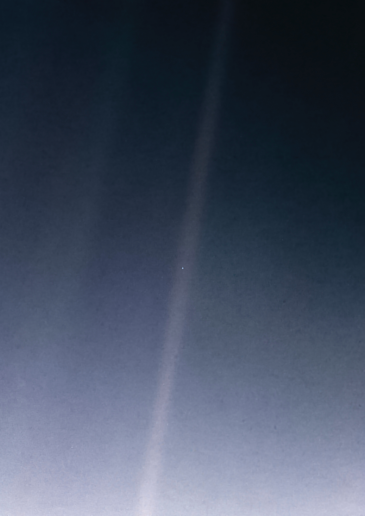
\includegraphics[width=\paperwidth,height=\paperheight,%
keepaspectratio]{images/palebluedotA4s.png}%
\vfill
}}}

%\usepackage[6-73,105-107]{pagesel}
\usepackage{tikz}
\usetikzlibrary{tikzmark}
\usetikzlibrary{arrows.meta}
% \usetikzlibrary{positioning}
% \newcommand{\tikzmark}[1]{\tikz[overlay,remember picture] \node (#1) {};}

\begin{document}
\AddToShipoutPicture*{\BackgroundPic}
\captiondelim{\quad}\captionnamefont{\footnotesize}\captiontitlefont{\footnotesize}
\selectlanguage{british}\frenchspacing

\begin{titlingpage}
\calccentering{\unitlength}
\begin{adjustwidth}{\unitlength}{-\unitlength}
  \centering
  % c6ddff % color of Earth in the Pale Blue Dot picture
  \color[HTML]{C6DDFF}
  \maketitle
\end{adjustwidth}
\end{titlingpage}
\killtitle

\calccentering{\unitlength}
\begin{adjustwidth*}{\unitlength}{-\unitlength}\thispagestyle{empty}
  \centering
  
\includegraphics[align=c,height=1em]{images/cc_by_sa.png} Licence

  \medskip
  P.G.L. Porta Mana \enskip\epost{\email{pgl}{portamana.org}}
  \\\href{https://orcid.org/0000-0002-6070-0784}{%
%\raisebox{0.5ex}{\protect%

\includegraphics[height=1ex]{pglpm_latex/orcid_32x32.png}%}
}%
\,{\footnotesize\url{https://orcid.org/0000-0002-6070-0784}}

\medskip

Typeset with \LaTeX%\ using 12\,pt Palatino and Optima fonts

\bigskip

Cover image: the \enquote{Pale Blue Dot} image of the Earth taken by Voyager~1,
\\from right outside Pluto's orbit\\
\url{https://science.nasa.gov/resource/voyager-1s-pale-blue-dot/}
\end{adjustwidth*}
\setcounter{page}{2}


%%%%%%%%%%%%%%%%%%%%%%%%%%%%%%%%%%%%%%%%%%%%%%%%%%%%%%%%%%%%%%%%%%%%%%%%%%%%
%%% Abstract
%%%%%%%%%%%%%%%%%%%%%%%%%%%%%%%%%%%%%%%%%%%%%%%%%%%%%%%%%%%%%%%%%%%%%%%%%%%%
% \abstractrunin
% \abslabeldelim{}
% \renewcommand*{\abstractname}{}
% \setlength{\absleftindent}{0pt}
% \setlength{\absrightindent}{0pt}
% \setlength{\abstitleskip}{-\absparindent}
% \begin{abstract}\labelsep 0pt%
%   \noindent Lecture notes on introductory mechanics and thermodynamics (ING175)
% % \\\noindent\emph{\footnotesize Note: Dear Reader
% %     \amp\ Peer, this manuscript is being peer-reviewed by you. Thank you.}
% % \par%\\[\jot]
% % \noindent
% % {\footnotesize PACS: ***}\qquad%
% % {\footnotesize MSC: ***}%
% %\qquad{\footnotesize Keywords: ***}
% \end{abstract}
\selectlanguage{british}\frenchspacing

%%%%%%%%%%%%%%%%%%%%%%%%%%%%%%%%%%%%%%%%%%%%%%%%%%%%%%%%%%%%%%%%%%%%%%%%%%%%
%%% Epigraph
%%%%%%%%%%%%%%%%%%%%%%%%%%%%%%%%%%%%%%%%%%%%%%%%%%%%%%%%%%%%%%%%%%%%%%%%%%%%
% \asudedication{\small ***}
% \vspace{\bigskipamount}
\setlength{\epigraphwidth}{0.67\linewidth}
% \epigraphtextposition{flushright}
% %\epigraphsourceposition{flushright}
\epigraphfontsize{\footnotesize}
\setlength{\epigraphrule}{0pt}
% % \epigraphposition{flushright}
% %\setlength{\beforeepigraphskip}{0pt}
%\setlength{\afterepigraphskip}{2em}



%%%%%%%%%%%%%%%%%%%%%%%%%%%%%%%%%%%%%%%%%%%%%%%%%%%%%%%%%%%%%%%%%%%%%%%%%%%%
%%% BEGINNING OF MAIN TEXT
%%%%%%%%%%%%%%%%%%%%%%%%%%%%%%%%%%%%%%%%%%%%%%%%%%%%%%%%%%%%%%%%%%%%%%%%%%%%
% \renewcommand{\cftchapterfont}{\hfill\bfseries}
% \renewcommand{\cftchapterleader}{}
% \renewcommand{\cftsectionfont}{\hfill\normalfont}
% \renewcommand{\cftcsectionleader}{}

\cleartooddpage
\phantomsection\pdfbookmark{\contentsname}{toc}
\setlength{\cftsectionnumwidth}{2.75em}
\tableofcontents*
\label{sec:toc}

\setcounter{chapter}{-1}


%%%%%%%%%%%%%%%%%%%%%%%%%%%%%%%%%%%%%%%%%%%%%%%%%%%%%%%%%%%%%%%%%%%%%%%%%%%%
%%% Preface
%%%%%%%%%%%%%%%%%%%%%%%%%%%%%%%%%%%%%%%%%%%%%%%%%%%%%%%%%%%%%%%%%%%%%%%%%%%%
\printpagenotes*
\cleartooddpage
\addchap{Preface}
\label{cha:preface}

\epigraph{I don't know what's the matter with people: they don't learn by understanding; they learn by some other way -- by rote, or something. Their knowledge is so fragile!\\[2\jot]
  Finally, I said that I couldn't see how anyone could be educated by this self-propagating system in which people pass exams, and teach others to pass exams, but nobody knows anything.}{R. P. Feynman \cites*{feynman1985_r1989}}

These notes are aimed at undergraduate students in Physics and in Engineering programmes, but graduate students may also find them useful.

You are probably aware of the variety of physics branches, such as mechanics, thermodynamics, chemistry, electromagnetics, fluid mechanics, statics, nuclear physics, and many others. Maybe you are acquainted with some of them. Probably you are also aware of the existence of different physical theories, like Newtonian Mechanics, General Relativity, Quantum Theory, which give different explanations and formulae for the same physical phenomena. Some physical theories are said to be more exact or more approximate than others; Newtonian mechanics, for instance, is an approximation of General Relativity. Does this wild variety of branches and theories also mean a wild variety of principles, methods, mathematical formulae -- which you'll have to learn if you want or need to study any particular branch or theory?

Yes, it does.

But there is also a core of very few principles that apply \emph{universally} to every branch and every theory known today, be it mechanics or thermodynamics, Newtonian Mechanics or General Relativity. If you learn these principles, you'll be able to \emph{immediately} work with, and understand, at least the general features of \emph{every} new physical discipline, phenomenon, or technology that you might meet.

\medskip

The main goal of these notes is to make you acquainted with this core of few physical principles.

How few are these principles? Around \emph{seven} (the exact number depends on how we arbitrarily group or separate them). This is the reason for the title of these notes. These seven principles are quite amazing for various reasons:
\begin{itemize}
\item They apply to \emph{every} physical phenomenon, as already mentioned.
\item Their meaning is very intuitive: each of them expresses a sort of budget.
\item They are responsible for, so to speak, \enquote{driving the universe forward in time}. More precisely, they are the basic principles that allow us to simulate and make predictions about physical phenomena.
\item Their mathematical formulation is \emph{exactly the same} in all our main approximate and exact theories, like Newtonian mechanics and General Relativity. This means that if you learn how to apply them to a tennis ball, then you are also able to apply them to a black hole.
\end{itemize}

\medskip

These universal principles are, obviously, expressed mathematically. Their consequences and applications can be studied, to some degree, by using analytical methods; that is, by methods involving mathematical operations that we can do by hand. But their most fascinating and practical applications need numerical methods, that is, methods involving programming and computer simulation.

In my opinion, if you learn how to apply these universal principles in simple simulations, then you also better understand their meaning and the way they work. For this reason these notes mainly take a computational approach. We shall learn how to implement these universal principles in simple computer code, and see the fun variety of physical phenomena they lead to. Scripts that accompany these notes can be found at
\begin{center}
  \url{https://pglpm.github.io/7wonders/}
\end{center}


\iftrue
\addsec{Thanks}
\label{sec:thanks}

I am deeply indebted to the students attending the courses ING\,175 and ING\,174 in 2024 at the Western Norway University of Applied Sciences (HVL) in Bergen. They allowed me to experiment presenting physics as done in these notes, and gave invaluable feedback about what's difficult and what's easy, what's unclear and what's clear, with many suggestions for improvement, and also moral support with their curiosity and enthusiasm. In particular I'd like to thank, in alphabetic order: %
Amalie Solberg Magnussen Rege, %
% Azzat Ammar Kouzi, %
Bodil Markhus, %
Carl Jakob Lis Sterner, %
% Cristopher Gerald Rojas, %
Dag Åsmund Ørnes, %
% Erlend Vitsø, %
Iver Thoresen Malme, %
Jonas Pytte, %
Josefine Björk Jarlesdottir Gjerde, %
Lars Magnus Birketveit, %
Leonard Rogardt Heldal, %
Miriam Osland, %
Nicolai Lindløkken, %
Nikolai Ringereide, %
Oda Skagsoset Kristiansen, %
Rebecca Sahlem, %
Rudi Nathaniel Stødle, %
Severin Johannessen, %
% Sondre Moa Risnes, %
% Stein Olav Løset Frey, %
Thea Tyssøy Jensen, %
Tim August Birkeland Christiansen, %
Vegard Aa Albretsen, %
William Sæther. %
Mats Øinas deserves a special thank for his thorough feedback, questions, suggestions, and encouragement.

A heartfelt thank goes to Yu-Chung Wang for his assistance in teaching and his feedback and continuous moral support.

Eternal gratitude and deepest esteem go to the teachers and Masters:
Gianni Astarita,
Ingemar Bengtsson,
Gunnar Bj{\"o}rk,
Alain Bossavit,
Percy W. Bridgman,
Robert Bringhurst,
William L. Burke,
Italo Calvino,
Yvonne Choquet-Bruhat,
Bernard D. Coleman,
C{\'e}cile DeWitt-Morette,
Margaret Dillard-Bleick,
Albert Einstein,
Leonhard Euler,
Jerald L. Ericksen,
Jean-Yves Girard,
{\'E}ric Gourgoulhon,
Theodore Hailperin,
Alexandr S. Holevo,
Thomas J. R. Hughes,
Edwin T. Jaynes,
Harold Jeffreys,
William E. Johnson,
Buster Keaton,
Attay Kovetz,
Jerrold E. Marsden,
Bogdan Mielnik,
Charles W. Misner,
Ingo M\"uller,
A. Ian Murdoch,
Robert Musil,
Friedrich Nietzsche,
Walter Noll,
David R. Owen,
Saitama,
Ivan Samoh{\'y}l,
Jan A. Schouten,
Miroslav {\v{S}}ilhav{\'y},
Kip S. Thorne,
Richard A. Toupin,
Clifford Truesdell,
Robert M. Wald,
John A. Wheeler,
Ludwig Wittgenstein.

Finally, thanks to the developers and maintainers of \LaTeX, Emacs, AUC\TeX, Open Science Framework, R, Octave, Python, LibreOffice, Inkscape, Sci-Hub, Libgen for making a free and impartial scientific exchange possible.
\fi

% \addsec{Guide to the text}
% \label{sec:guide}
%
% \addsubsec{Physics prerequisites}
% \label{sec:guide_physics}
%
% Just some vague reminiscences of secondary/high-school physics should be enough.
%
% It can be beneficial if you are familiar with basic physics notions like \emph{velocity}, \emph{mass}, \emph{force}, and similar ones.
%
% \addsubsec{Maths prerequisites}
% \label{sec:guide_maths}
%
% \begin{itemize}
% \item Working familiarity with algebra, its operations and their properties.
% \item Working familiarity with solving equations and inequalities, linear and non-linear.
% \item Working familiarity with the study of functions of one real variable.
% \item Working familiarity with derivatives.
% \item Understanding of what an integral is, even if you won't be required to solve integrals.
% \item Working familiarity with vector calculus.
% \item Some familiarity with functions of many variables.
% \item Understanding of what partial derivatives are.
% \end{itemize}
%
%
% \addsubsec{Programming prerequisites}
% \label{sec:guide_program}
%
% \begin{itemize}
% \item Knowing what a computer program is.
% \item Working familiarity with variables in a computer program.
% \item Working familiarity with \texttt{for}- and \texttt{while}-loops.
% \item Working familiarity with outputting and plotting the results of a computer program.
% \end{itemize}
%
%
% \addsubsec{Structure of this text}
% \label{sec:guide_text}
%
% \subsubsection{\faIcon{hand-point-right}\enskip Graphical devices}
%
% The text includes the following graphical devices:
% \begin{itemize}[para]
% \item Important notions and definitions are also given in \textbf{boldface}.
%
% \item\label{sec:self-reference}
%   % \subsection*{\faIcon{hand-point-right}\enskip References to previous topics}
%
% The side margins often report clickable references to \autoref{sec:self-reference}{previous topics, emphasized in blue}.
%
% \item Important-notion boxes:
%   \begin{definition}{Some important notion or definition}
%     This is a definition or explanation of Something.
%   \end{definition}
% \item Warnings and important points that require careful thinking:
%   % \colorlet{shadecolor}{red}
%   % \begin{shaded}
%   %   Something you must be careful about.
%   % \end{shaded}
%   \begin{warning}[Careful!]
%     Something you must be careful about.
%   \end{warning}
% \item Exercises:
%   \begin{exercise}
%     This isn't really an exercise
%   \end{exercise}
% % \item Possible objections you might be thinking about:
% %   \begin{critique}[This isn't right!]
% %     I have an objection here.
% %   \end{critique}
% \item Discussions and connections with more advanced physics:
%   \begin{extra}{How things really are in quantum physics}
%     Just for your curiosity.
%   \end{extra}
% \end{itemize}
%
% \subsubsection{\faIcon{hand-point-right}\enskip Side pictures and quotes}
%
% \marginpar{\centering%
% 
\includegraphics[align=c,width=0.5\linewidth]{images/saitama_image.png}%
% \\[\jot]\footnotesize\flushleftright{\color{green}%
% This is an image of Saitama, which actually has nothing to do with the text on the left.}
% }%
% Pictures, graphs, or quotes related to the material are displayed on the right.
%
%
% \subsubsection{\faIcon{hand-point-right}\enskip Hyperlinks and bibliography}
%
% Some words are hyperlinks, like this one about \furl{https://onepunchman.fandom.com}{One Punch Man}; you also recognize them because they have a little footnote number. The links' URLs are listed at the end of each chapter, just in case you're reading a printed copy and wonder what the link was.
%
% \medskip
%
% The text gives bibliographic references, like \enquote{\cites{einstein1905c}}, to scientific literature. The references are listed in the final Bibliography on page~\pageref{sec:biblio}.
%
% These references are given for two reasons:
% \begin{itemize}
% \item For your own curiosity.
%
% \item
% \marginpar{\vspace{-3\baselineskip}\footnotesize\raggedright\color{mpcolor}\emph{%
% \enquote{Believe nothing, O monks, merely because you have been told it, or because it is traditional, or because you yourselves have imagined it. Do not believe what your teacher tells you merely out of respect for the teacher.}}
% \\[\jot](attributed to Gautama Buddha)
% }%
% To back up what's written in the text.
% In science you should not believe something just because you've read it somewhere. You should, as much as possible, \emph{go and check for yourself how the logic behind the statement is proved and what is the experimental evidence behind the statement}.
% \end{itemize}
%
% \subsubsection{\faIcon{hand-point-right}\enskip Notation and terminology}
%
% Mathematical notation, as well as notation for physical dimensions, strictly follows the standards given by the \furl{https://www.nist.gov/pml/special-publication-811}{International System of Units (SI)}, listed for example in \cites{iso2009} and \cites{iso2019}.


\printpagenotes*
\cleartooddpage
\chapter{Overview}
\label{cha:overview}

\epigraph{\enquote{What you do in this world is a matter of no consequence,} returned my companion, bitterly. \enquote{The question is, what can you make people believe that you have done?\textellipsis}}{Sherlock Holmes (A. C. Doyle) \cites*{doyle1887}}

\section{The plan of these notes}

After some very general remarks about physics, we recall the notions of \textbf{physical quantity}, unit, and physical dimension. This is really just a reminder; it's assumed that you are already familiar with these general notions.

We then survey two cardinal physical notions: \textbf{time} and \textbf{space}. We briefly examine their fascinating nature as we today understand it. The notion of \textbf{coordinate system} is also introduced.

Thereafter we take an overview of the main seven physical quantities we shall work with: \textbf{matter}, \textbf{energy-mass}, \textbf{momentum}, \textbf{angular momentum}, \textbf{entropy},  \textbf{electric charge}, \textbf{magnetic flux}, discussing some features common to all of them. Other important quantities such as temperature are also introduced.

The most important feature of the main seven quantities is that we can measure their amount within any volume, and the amount that passes through any surface. We therefore study the intuitive ideas of \textbf{control volume} and \textbf{volume content}, \textbf{control surface} and \textbf{flux}, and \textbf{supply}.

At this point the stage is ready for the introduction of seven physical laws which are just expressions of \textbf{balances} of volume contents, fluxes, and supplies of the seven quantities introduced earlier. These seven balance laws are \textbf{universal}. They are connected by mathematical expressions called \textbf{constitutive relations}, which are not universal but depend on the particular physical phenomenon, and on the particular physical theory we use to describe it.

The balance laws are the ones that allow us to predict how the values of different quantities change with time. We show this by exploiting them to code numerical simulations that can in principle be done for any physical system. The role that constitutive relations have in connecting the seven balances also becomes quite clear in the simulation code.

The seven universal balances are then examined in turn. For each balance, we study some constitutive relations that are often used together with it, as well as some of its physical applications.


\section{Prerequisites}
\label{sec:guide_physics}

\subsection{Physics}

Just some vague reminiscences of secondary/high-school physics should be enough. It can be beneficial if you are familiar with basic physics notions like \emph{velocity}, \emph{mass}, \emph{force}, and similar ones.

\subsection{Maths}

\begin{itemize}
\item Working familiarity with algebra, its operations and their properties.
\item Working familiarity with solving equations and inequalities, linear and non-linear.
\item Working familiarity with the study of functions of one real variable.
\item Working familiarity with derivatives.
\item Understanding of what an integral is, even if you won't be required to solve integrals.
\item Working familiarity with vector calculus.
\item Some familiarity with functions of many variables.
\item Understanding of what partial derivatives are.
\end{itemize}


\subsection{Programming}

\begin{itemize}
\item Knowing what a computer program is.
\item Working familiarity with variables in a computer program.
\item Working familiarity with \texttt{for}- and \texttt{while}-loops.
\item Working familiarity with outputting and plotting the results of a computer program.
\end{itemize}


\section{Features of the text}
\label{sec:guide_text}

% \subsubsection{\texorpdfstring{\faIcon{hand-point-right}\enskip}{}Graphical devices}
\subsection{Graphical devices}

The text includes the following graphical devices:
\begin{itemize}[para]
\item Important concepts and definitions are also given in \textbf{boldface}.

% \item\label{sec:self-reference}
%   % \subsubsection{\faIcon{hand-point-right}\enskip References to previous topics}
% 
% Clickable references to previous or future topics are often given in \autoref{sec:self-reference}{blue text and round brackets like this:}.

\item Important-concept boxes:
  \begin{definition}{Some important notion or definition}
    This is a definition or explanation of Something.
  \end{definition}
\item Warnings and important points that require careful thinking:
  % \colorlet{shadecolor}{red}
  % \begin{shaded}
  %   Something you must be careful about.
  % \end{shaded}
  \begin{warning}[Careful!]
    Something you must be careful about.
  \end{warning}
\item Exercises:
  \begin{exercise}
    This isn't really an exercise
  \end{exercise}
% \item Possible objections you might be thinking about:
%   \begin{critique}[This isn't right!]
%     I have an objection here.
%   \end{critique}
\item Discussions and connections with more advanced physics:
  \begin{extra}{How things really are in quantum physics}
    Just for your curiosity.
  \end{extra}
\end{itemize}

% \subsubsection{\texorpdfstring{\faIcon{hand-point-right}\enskip}{}Side figures and quotes}
\subsection{Side figures and quotes}

\marginpar{\vspace{-4\baselineskip}\footnotesize\centering%

\includegraphics[width=0.5\linewidth]{images/saitama_image.png}%
\\[\jot]\flushleftright{\color{green}%
This is an image of Saitama, which actually has nothing to do with the text on the left.}
}%
Figures, graphs, or quotes related to the material are displayed on the right.


% \subsubsection{\texorpdfstring{\faIcon{hand-point-right}\enskip}{}Cross-references}
\subsection{Cross-references}

\marginpar{\vspace{1\baselineskip}\footnotesize%
  \flushleftright\color{green}%
  The symbol \enquote*{\,\sect\,} stands for \enquote*{section}.%
}%
The text gives cross-references to the main section where a topic was or will be discussed. Cross-references appear as an eye icon followed by sectioning number and page in round brackets, like this cross-reference to \autoref{sec:conservation_laws}{conservation laws}.


% \subsubsection{\texorpdfstring{\faIcon{hand-point-right}\enskip}{}Hyperlinks and bibliography}
\subsection{Hyperlinks and bibliography}

Some pieces of text are hyperlinks, like this one about \furl{https://onepunchman.fandom.com}{One Punch Man}. You recognize them from their different colour and from the little footnote number that follows them. The links' URLs are also listed at the end of each chapter, in case you're reading a printed copy of these notes.

\medskip

The text gives bibliographic references, like \enquote{\cites{einstein1905c}}, to scientific literature. The references are listed in the final Bibliography on page~\pageref{sec:biblio}. Bibliographic references are given for two reasons:
\begin{itemize}
\item For your own curiosity.

\item \marginpar{\vspace{-1\baselineskip}\footnotesize\raggedright\color{mpcolor}\emph{%
      \enquote{Believe nothing, O monks, merely because you have been told it, or because it is traditional, or because you yourselves have imagined it. Do not believe what your teacher tells you merely out of respect for the teacher.}} \\[\jot](attributed to Gautama Buddha)%
  }%
  To back up what's written in the text. In science you should not believe something just because you've read it somewhere. You should, as much as possible, \emph{go and check for yourself the logic and the experimental evidence behind the statement}.
\end{itemize}

\section{Code for numerical simulations}
\label{sec:code}

\subsection{Octave}
The scripts for numerical simulations presented in the text are written in \furl{https://octave.org}{\emph{Octave}} (they should also work in \furl{https://mathworks.com/products/matlab.html}{\emph{MATLAB}}). Why \emph{Octave}? Several reasons:
\begin{itemize}
\item It's free and open source.
\item It runs on all major operating systems.
\item It includes a graphical user interface and development environment.
\item It allows the specification of objects like vectors in a way very similar to physics and maths notation.
\item It doesn't need extra packages.
\item Its code can be copied \amp\ pasted without worrying about losing leading whitespace.
\end{itemize}
Keep in mind that in Octave a trailing semicolon \textcolor{codecolour}{\texttt{;}} prevents the result of an operation to be printed to the console or to output.

\subsection{Python}

\furl{https://www.python.org}{\emph{Python}} versions of the scripts are also usually given, linked on the margin. They need the \furl{https://numpy.org}{\emph{NumPy}} and  \furl{https://matplotlib.org}{\emph{Matplotlib}} packages. The Python scripts should work on \furl{https://matplotlib.online}{\texttt{matplotlib.online}}.

\subsection{Code colours}

The scripts usually present two colours:
\begin{itemize}
\item \textcolor{codecolour}{Blue lines} are strictly related to the physical simulation. 
\item \textcolor{grey}{Grey lines} take care of auxiliary operations, like plotting the results or saving them to file.
\end{itemize}

% \subsubsection{\texorpdfstring{\faIcon{hand-point-right}\enskip}{}Notation and terminology}
\section{Notation and terminology}
\label{sec:list_symbols}

Mathematical notation follows as much as possible the standards given by the \furl{https://www.nist.gov/pml/special-publication-811}{International System of Units (SI)}, listed for example in \cites{iso2009} and \cites{iso2019}. One slight exception are \autoref{sec:units}{physical dimensions}, whose notation will be explained in that section.

\medskip


In physics, engineering, and most other scientific fields \emph{there is no universal standard for symbols}. It's therefore important that you \textbf{focus on the concept} that a symbol stands for, rather than the symbol itself. Otherwise you'll face many difficulties reading literature and other scientists' reports.

The present notes try to use as much as possible the symbols recommended by the \furl{https://www.iso.org}{International Organization for Standardization (ISO)}, which are often also adopted by other international bodies like the \furl{https://www.bipm.org}{International Bureau of Weights and Measures (BIPM)}, the \furl{https://www.ieee.org}{Institute of Electrical and Electronics Engineers (IEEE)}, or the \furl{https://iupac.org}{International Union of
  Pure and Applied Chemistry (IUPAC)}. Some changes are unavoidable, because different disciplines often use the same symbol for different quantities. For instance, the symbol \enquote*{$E$} is used in many fields for \enquote*{energy}, in mechanics for the \enquote*{Young modulus} (a mechanical characteristic of elastic materials), in electromagnetics for the \enquote*{magnitude of the electric field}.

The most common symbols used in the present notes are listed in table~\ref{tab:symbols} on page~\pageref{tab:symbols}.

% \printpagenotes*
% \cleartooddpage
% \addchap{List of symbols}
% \label{cha:list_symbols}


\begin{table}[p]
 \centering
  \footnotesize
 \caption{List of common symbols}
  \label{tab:symbols}
  \begin{tabularx}{1.0\linewidth}{ll}
    \rlap{\textit{(Greek symbols)}}&
    \\%[\jot]
    $\yGG$ & gravitational constant
    \\
    $\yvis$ & viscosity coefficient
    \\
    $\yfrik$ & coefficient of kinetic friction
    \\
    $\yfris$ & coefficient of static friction
    \\
    $\yB$ & entropy flux
    \\
    $\yrho$ & molar mass
    \\
    $\yH$ & \energym\ flux
    \\
    $\yOm$ & angular-velocity matrix
    \\
    $\yo$ & angular-velocity vector
    \\[1.5\jot]
    \rlap{\textit{(Latin symbols)}}&
    \\%[\jot]
    $A$ & usually: area; in some contexts: just a coefficient
    \\
    $\ya$ & matter supply
    \\
    $\yBf$ & magnetic flux
    \\
    $C$ & usually: molar heat capacity; in some contexts: just a coefficient
    \\
    $\yc$ & usually: speed of light; in some contexts: just a coefficient
    \\
    $\yE$ & \energym\ content
    \\
    $\yEv$ & electric potential difference (electric tension)
    \\
    $\yF$ & momentum flux (surface force)
    \\
    $\yG$ & momentum supply (volume force)
    \\
    $\yg$ & acceleration vector of free fall
    \\
    $\yhea$ & surface coefficient of heat transfer
    \\
    $\yIc$ & tensor of inertia (with respect to centre of \masse)
    \\
    $\yI$ & electric current
    \\
    $\yJ$ & matter flux
    \\
    $k$ & elastic constant
    \\
    $\yL$ & angular-momentum content
    \\
    $\yM$ & angular-momentum flux (surface torque)
    \\
    $\ym$ & \masse\ content, typically at rest
    \\
    $\yN$ & matter content (amount of substance)
    \\
    $\yP$ & momentum content
    \\
    $p$ & pressure
    \\
    $\yQ$ & heat flux
    \\
    $\yC$ & electric-charge content
    \\
    $R$ & usually: molar gas constant; in some contexts: radius
    \\
    $\yR$ & \energym\ supply
    \\
    $\yr$ & coordinate-position vector
    \\
    $\yS$ & entropy content
    \\
    $\yT$ & thermodynamic temperature (in kelvins)
    \\
    $\yto$ & angular-momentum supply (volume torque)
    \\
    $t$ & coordinate time
    \\
    $\yU$ & internal energy
    \\
    $V$ & volume
    \\
    $\yv$ & coordinate-velocity vector
    \\
    $x$ & position coordinate, typically horizontal
    \\
    $y$ & position coordinate, typically horizontal
    \\
    $z$ & position coordinate, typically vertical
  \end{tabularx}
\end{table}


\printpagenotes*
\cleartooddpage
\chapter{Physics, quantities, units}
\label{cha:physics_quantities_units}

\epigraph{Philosophy is written in this grand book, the universe, which stands continually open to our gaze. But the book cannot be understood unless one first learns to comprehend the language and read the letters in which it is composed. It is written in the language of mathematics, and its characters are triangles, circles, and other geometric figures without which it is humanly impossible to understand a single word of it.}{G. Galilei \cites*{galilei1623}}

\section{Physics?}
\label{sec:physics_general}

% \section{Magic}
% \label{sec:magic}

If you think about it, many things we ordinarily do every day are some sort of magic. Think of how you can instantaneously see and speak with a person living on another continent, in real time, using just a small widget in the palm of your hand. Think of how you can instantaneously see where you are on the Earth, using the same widget. Think of how fast you can go to another country, by flying in a huge metal thing. Think of how you can command and interact with a purely fictitious animated world when you play on your computer. The list can go on forever. Other things are luckily less ordinary, but still inspire a lot of awe: think of the devastating power unleashed by something roughly as small as a tennis ball, in an atomic bomb.

We can do these astonishing things thanks to our understanding of how the world works. That's Physics.

\medskip

Many things can be said and have been said about science and physics. Rather than repeating what's been already written in many excellent books, I invite you to take a break here and go read their introductions. Choose as you please; compare what they say; don't limit yourself to popular books.

% \begin{center}
%   \textellipsis
%   \textellipsis
%   \textellipsis
% \end{center}



\section{What is \enquote{fundamental} physics?}
\label{sec:fundamental_physics}

But what's the \enquote{ultimate} goal of physics? What's \enquote{fundamental} physics? The answer to this question is again subjective -- also in this case physics lets you express your proclivities and personality. In the history of physics one can probably identify two main conceptions of \enquote{fundamental} physics.

For some physicists it is about finding the ultimate building blocks, so that one day we can say \enquote{\textellipsis and these are the constituents, and they obey these equations}. The history of physics seems to show that this goal is overturned every few generations. And yet every generation says \enquote{\emph{Now} we almost have the complete picture -- it's right behind the corner. It's true that previous generations thought they almost had it, and turned out to be wrong. But \emph{this time} is different, this time we have the real deal!}. The theoretical and particle physicist \furl{https://www.physics.lbl.gov/rememberinggeoffreychew/}{Geffrey Chew} depicted this situation as in \fig\,\ref{fig:chew1}. For this reason some physicists are a little sceptical about this goal; maybe it's a never-ending structure, with surprises at every deeper look.

So for other physicists fundamental physics is about finding some point of view or mathematical structure that is rich enough to make useful predictions, and yet flexible enough to accommodate any new patterns or objects that we might discover. In a manner of speaking, it is about finding \enquote{patterns of patterns} or \enquote{laws about physical laws}.

The two conceptions above are not mutually exclusive, and both are always pursued, even if time-changing fashions may emphasize the one or the other.

In these notes we take a point of view slightly closer to the second conception. This will also be reflected in the main division between two kinds of physical laws that we'll draw in \chap~\ref{cha:laws}.


\begin{figure}[p]
  \centering
  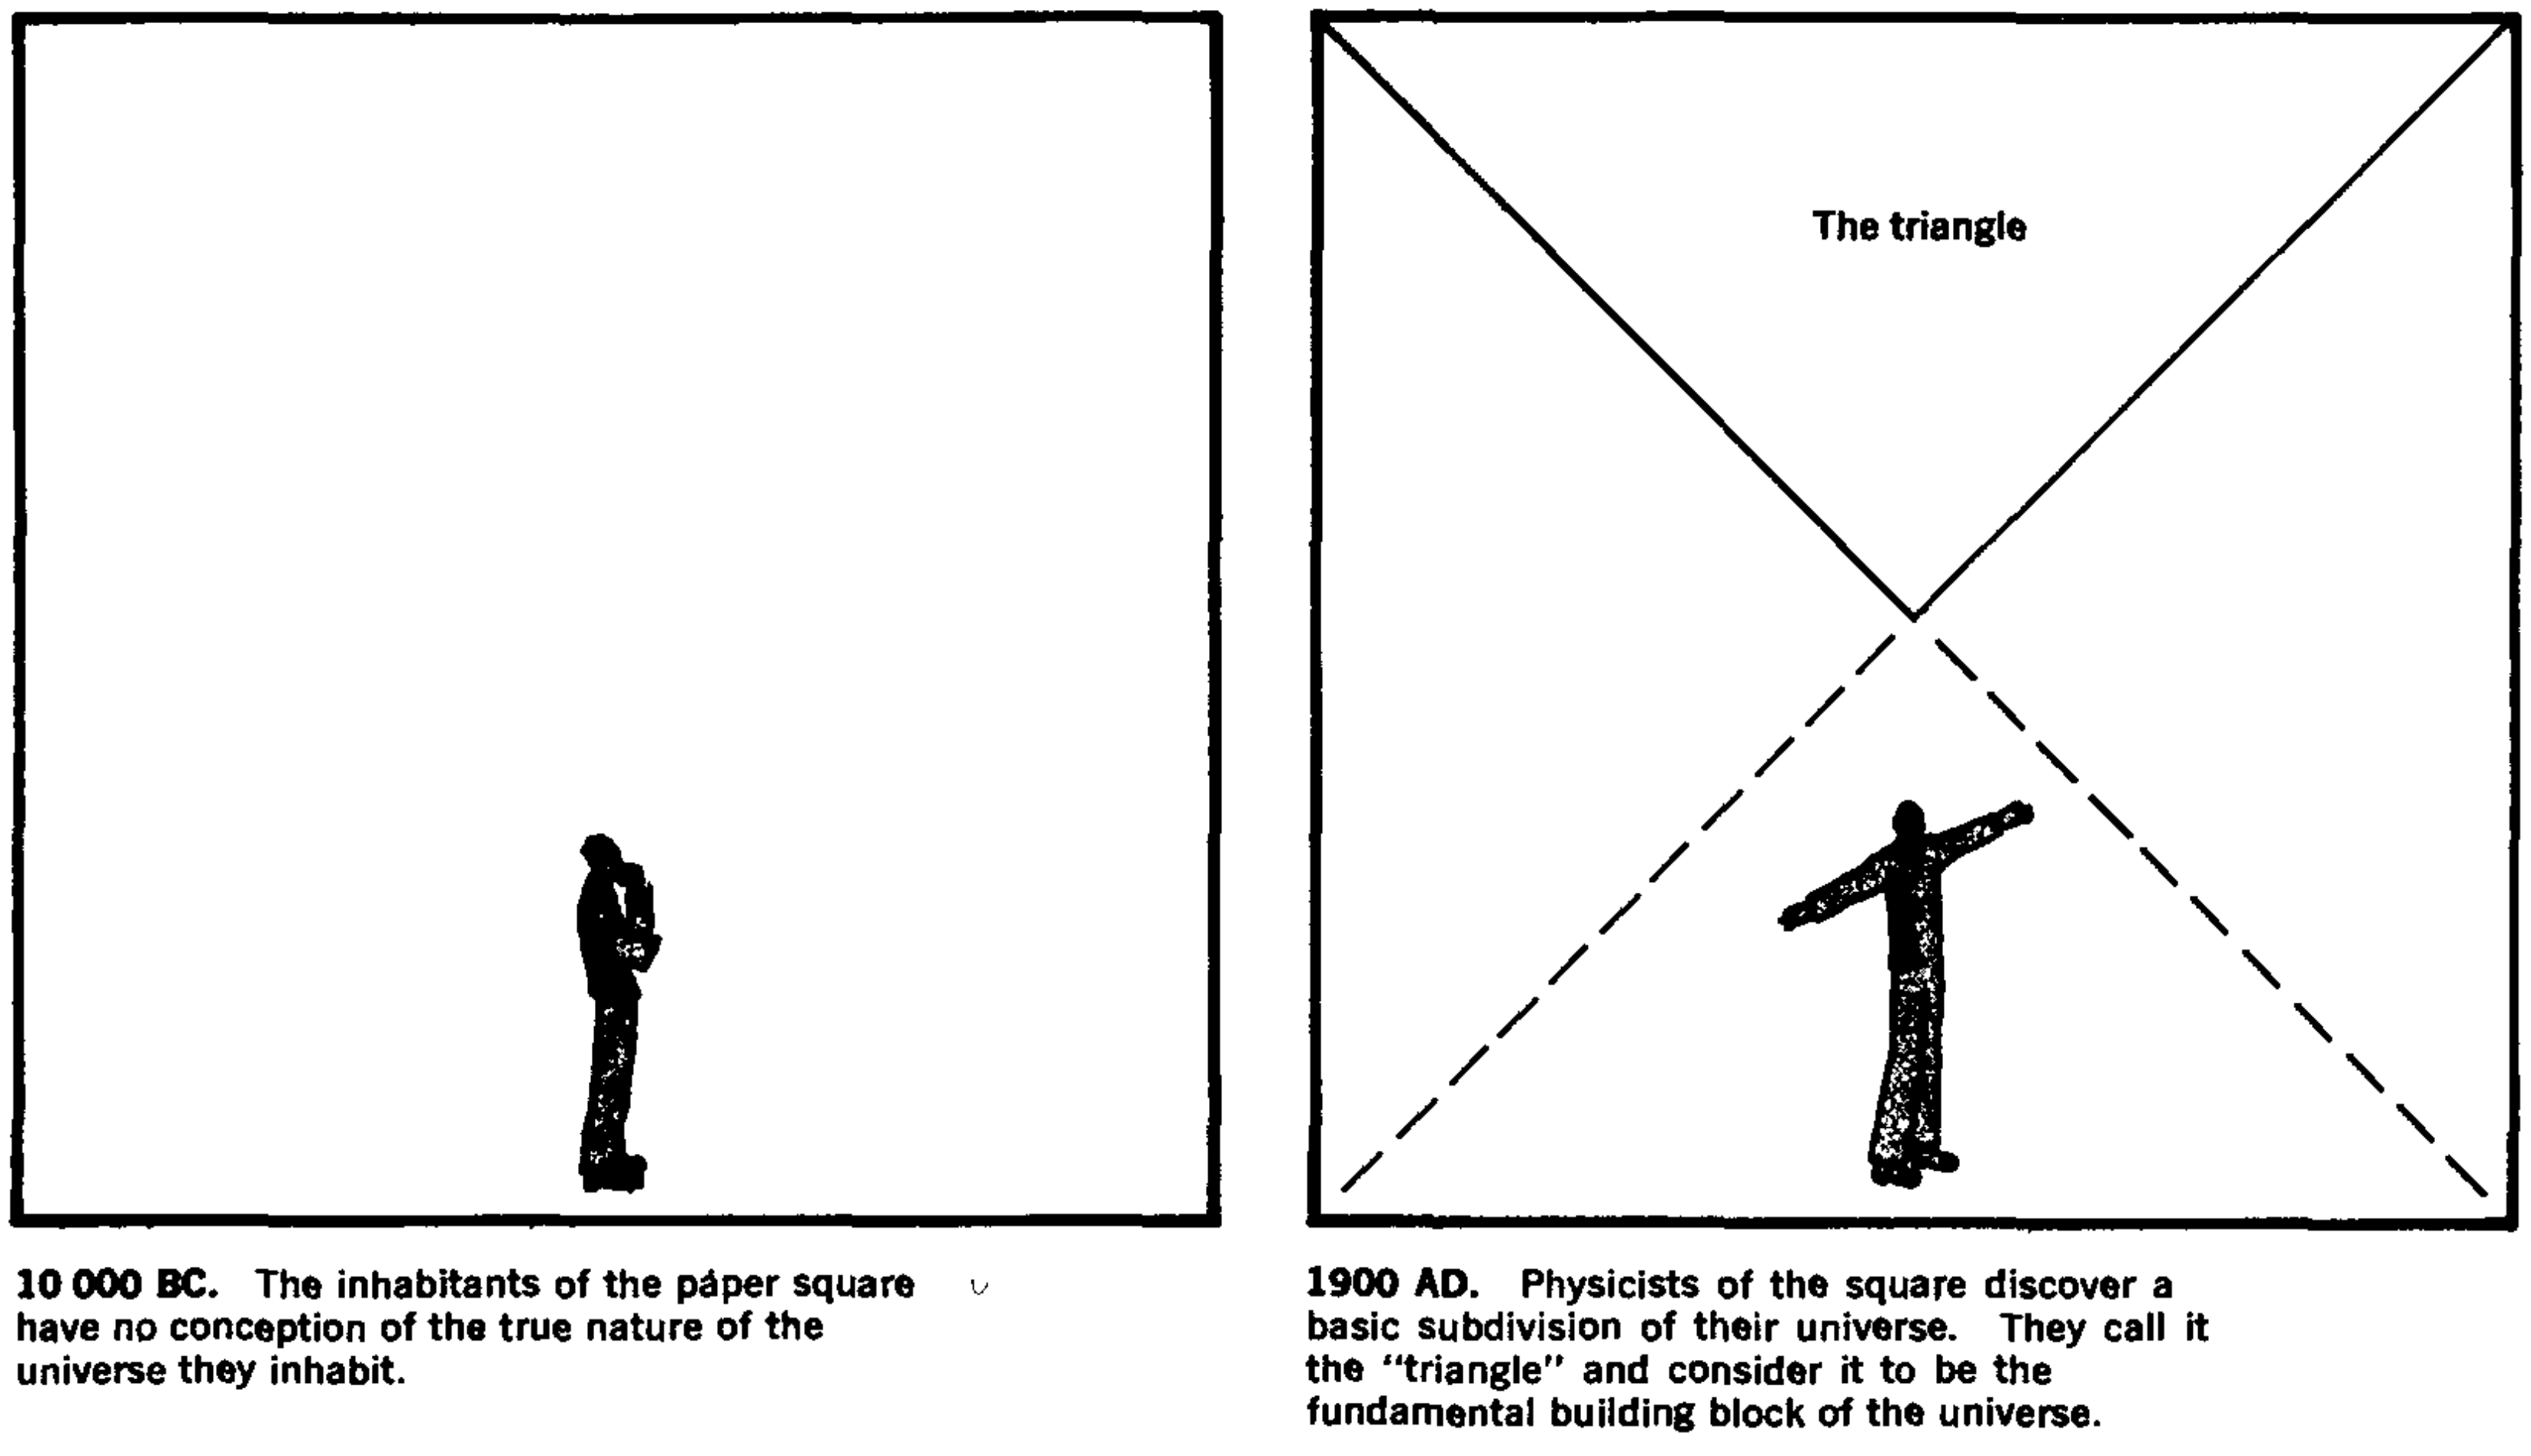
\includegraphics[width=1.2\textwidth]{images/chew1.png}
  \\[1em]  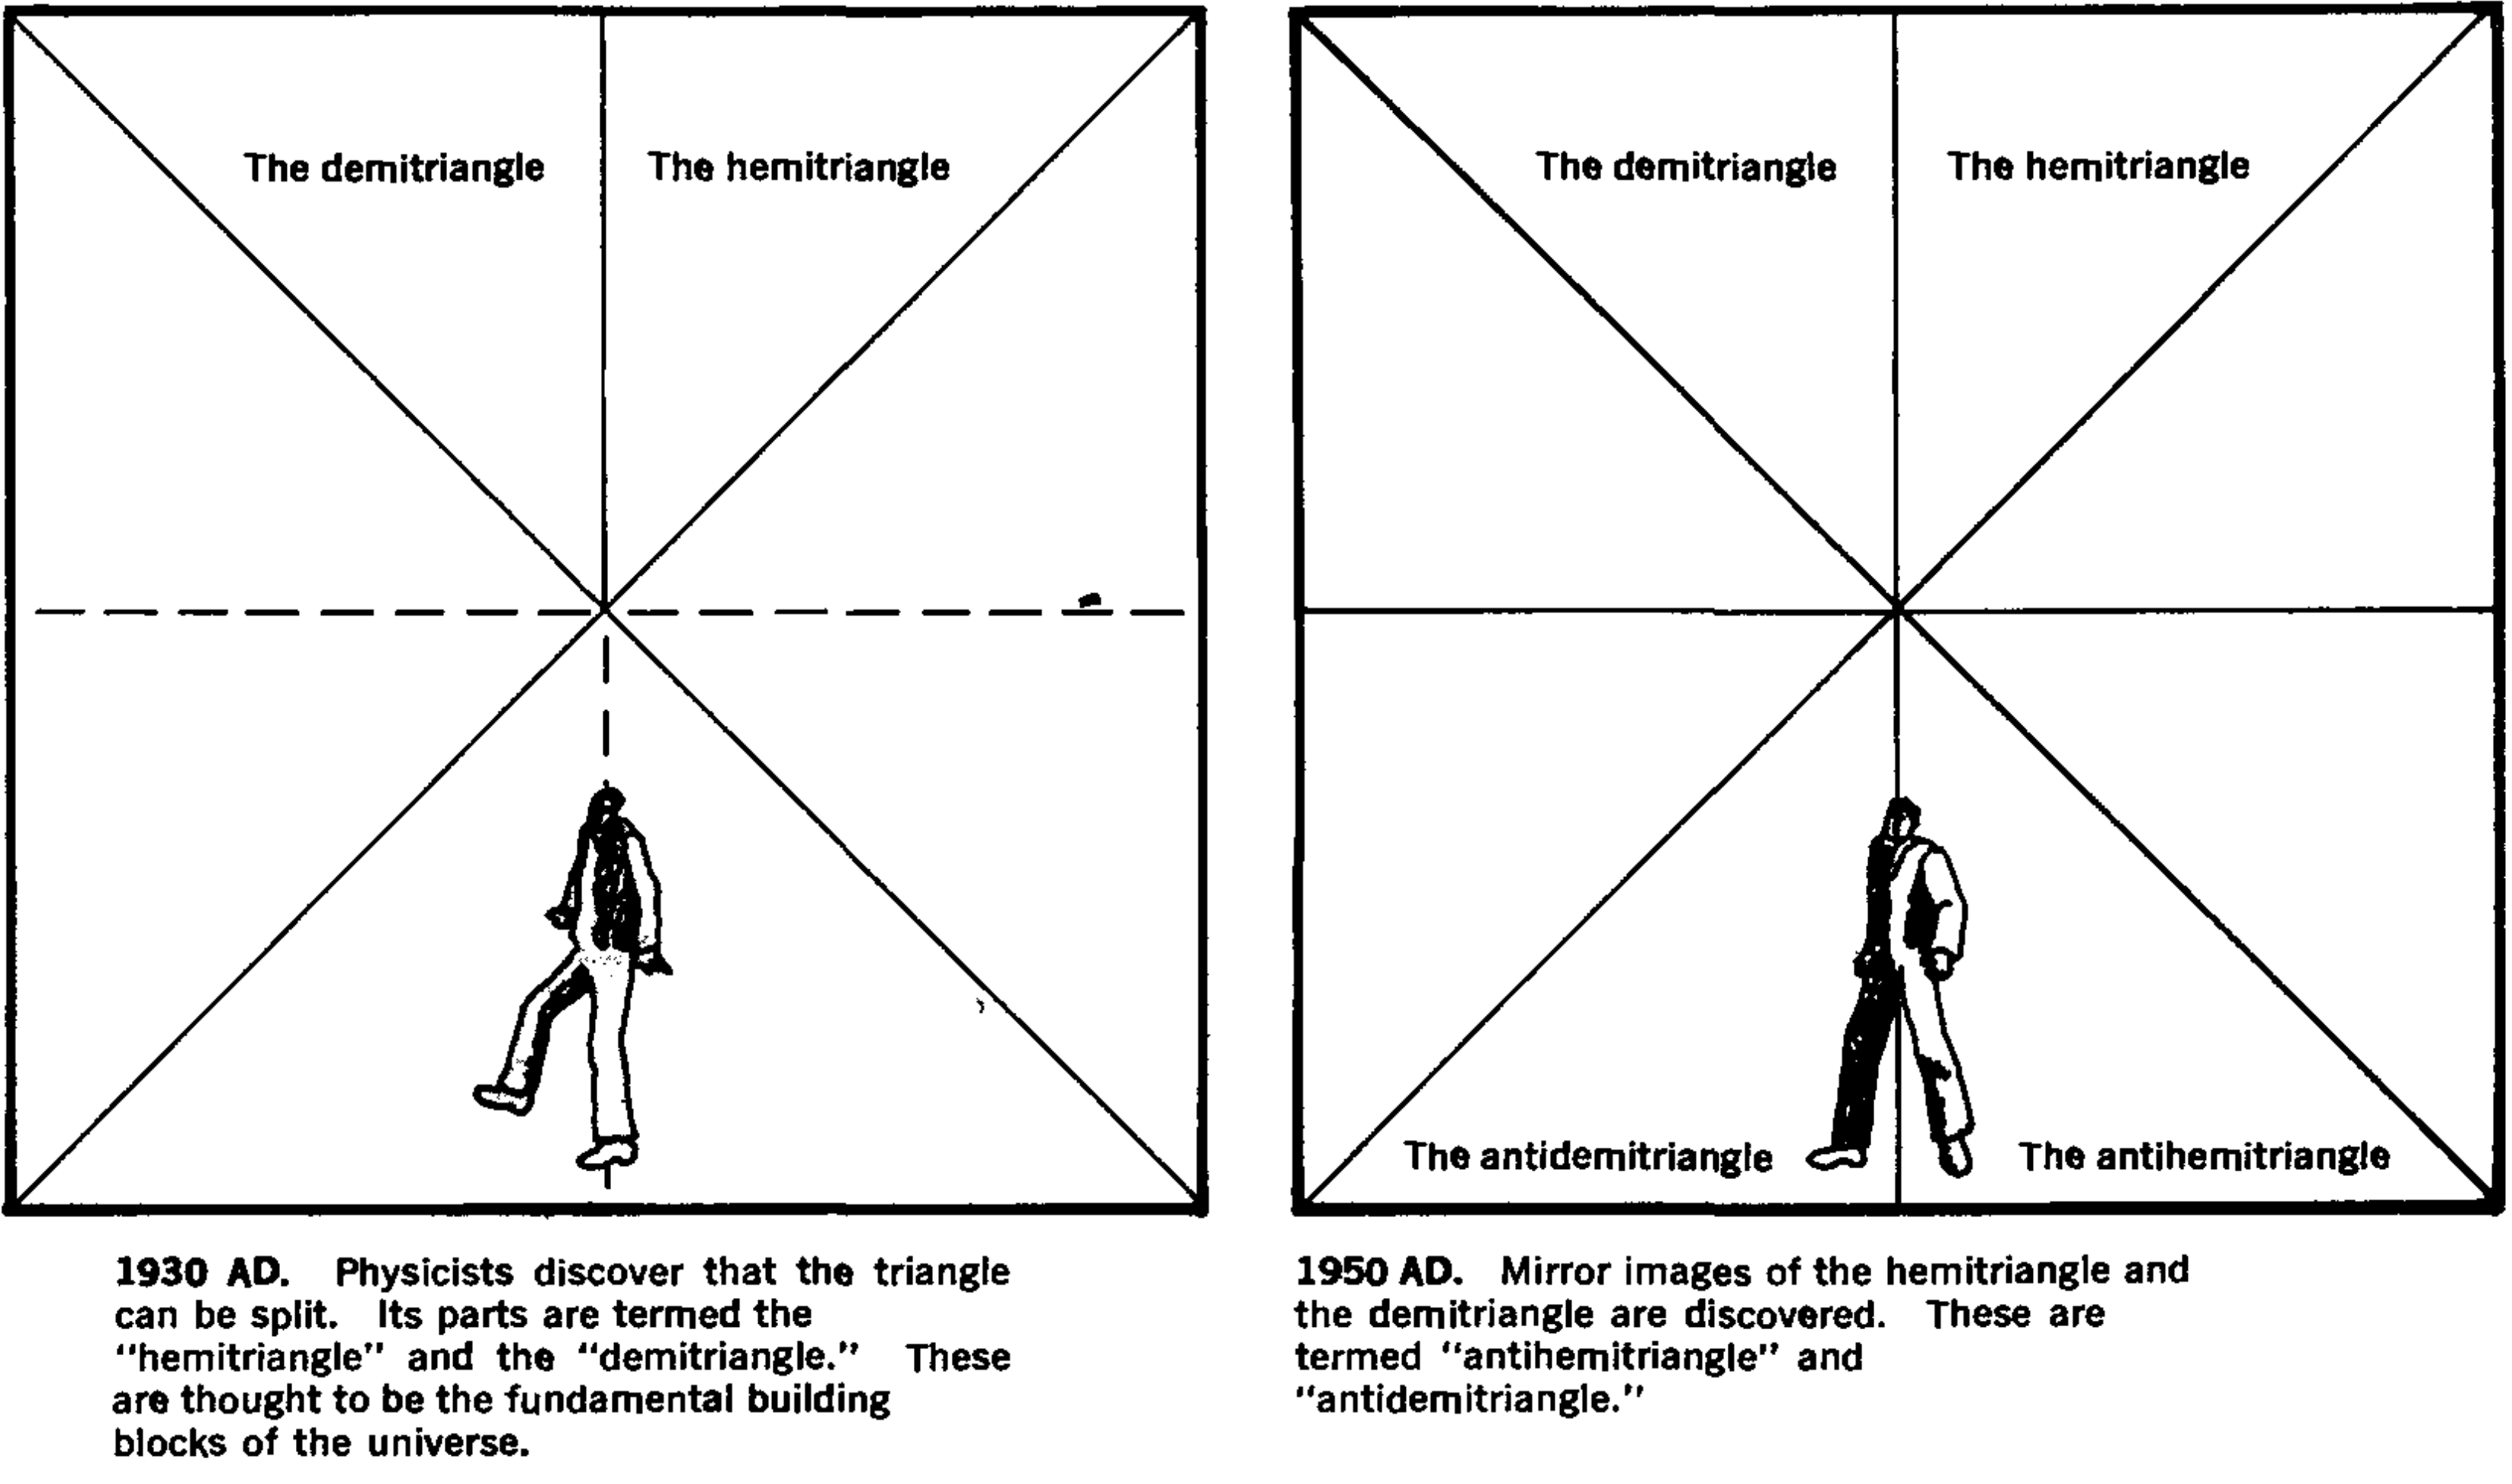
\includegraphics[width=1.2\textwidth]{images/chew2.png}
  \caption{(Continues on p.~\pageref{fig:chew2}) \emph{The progress of \enquote{fundamental} physics}, from \cites{chew1970} as reproduced in \cites{truesdell1984_r1987}}
  \label{fig:chew1}
\end{figure}
\begin{figure}[p]
  \centering
  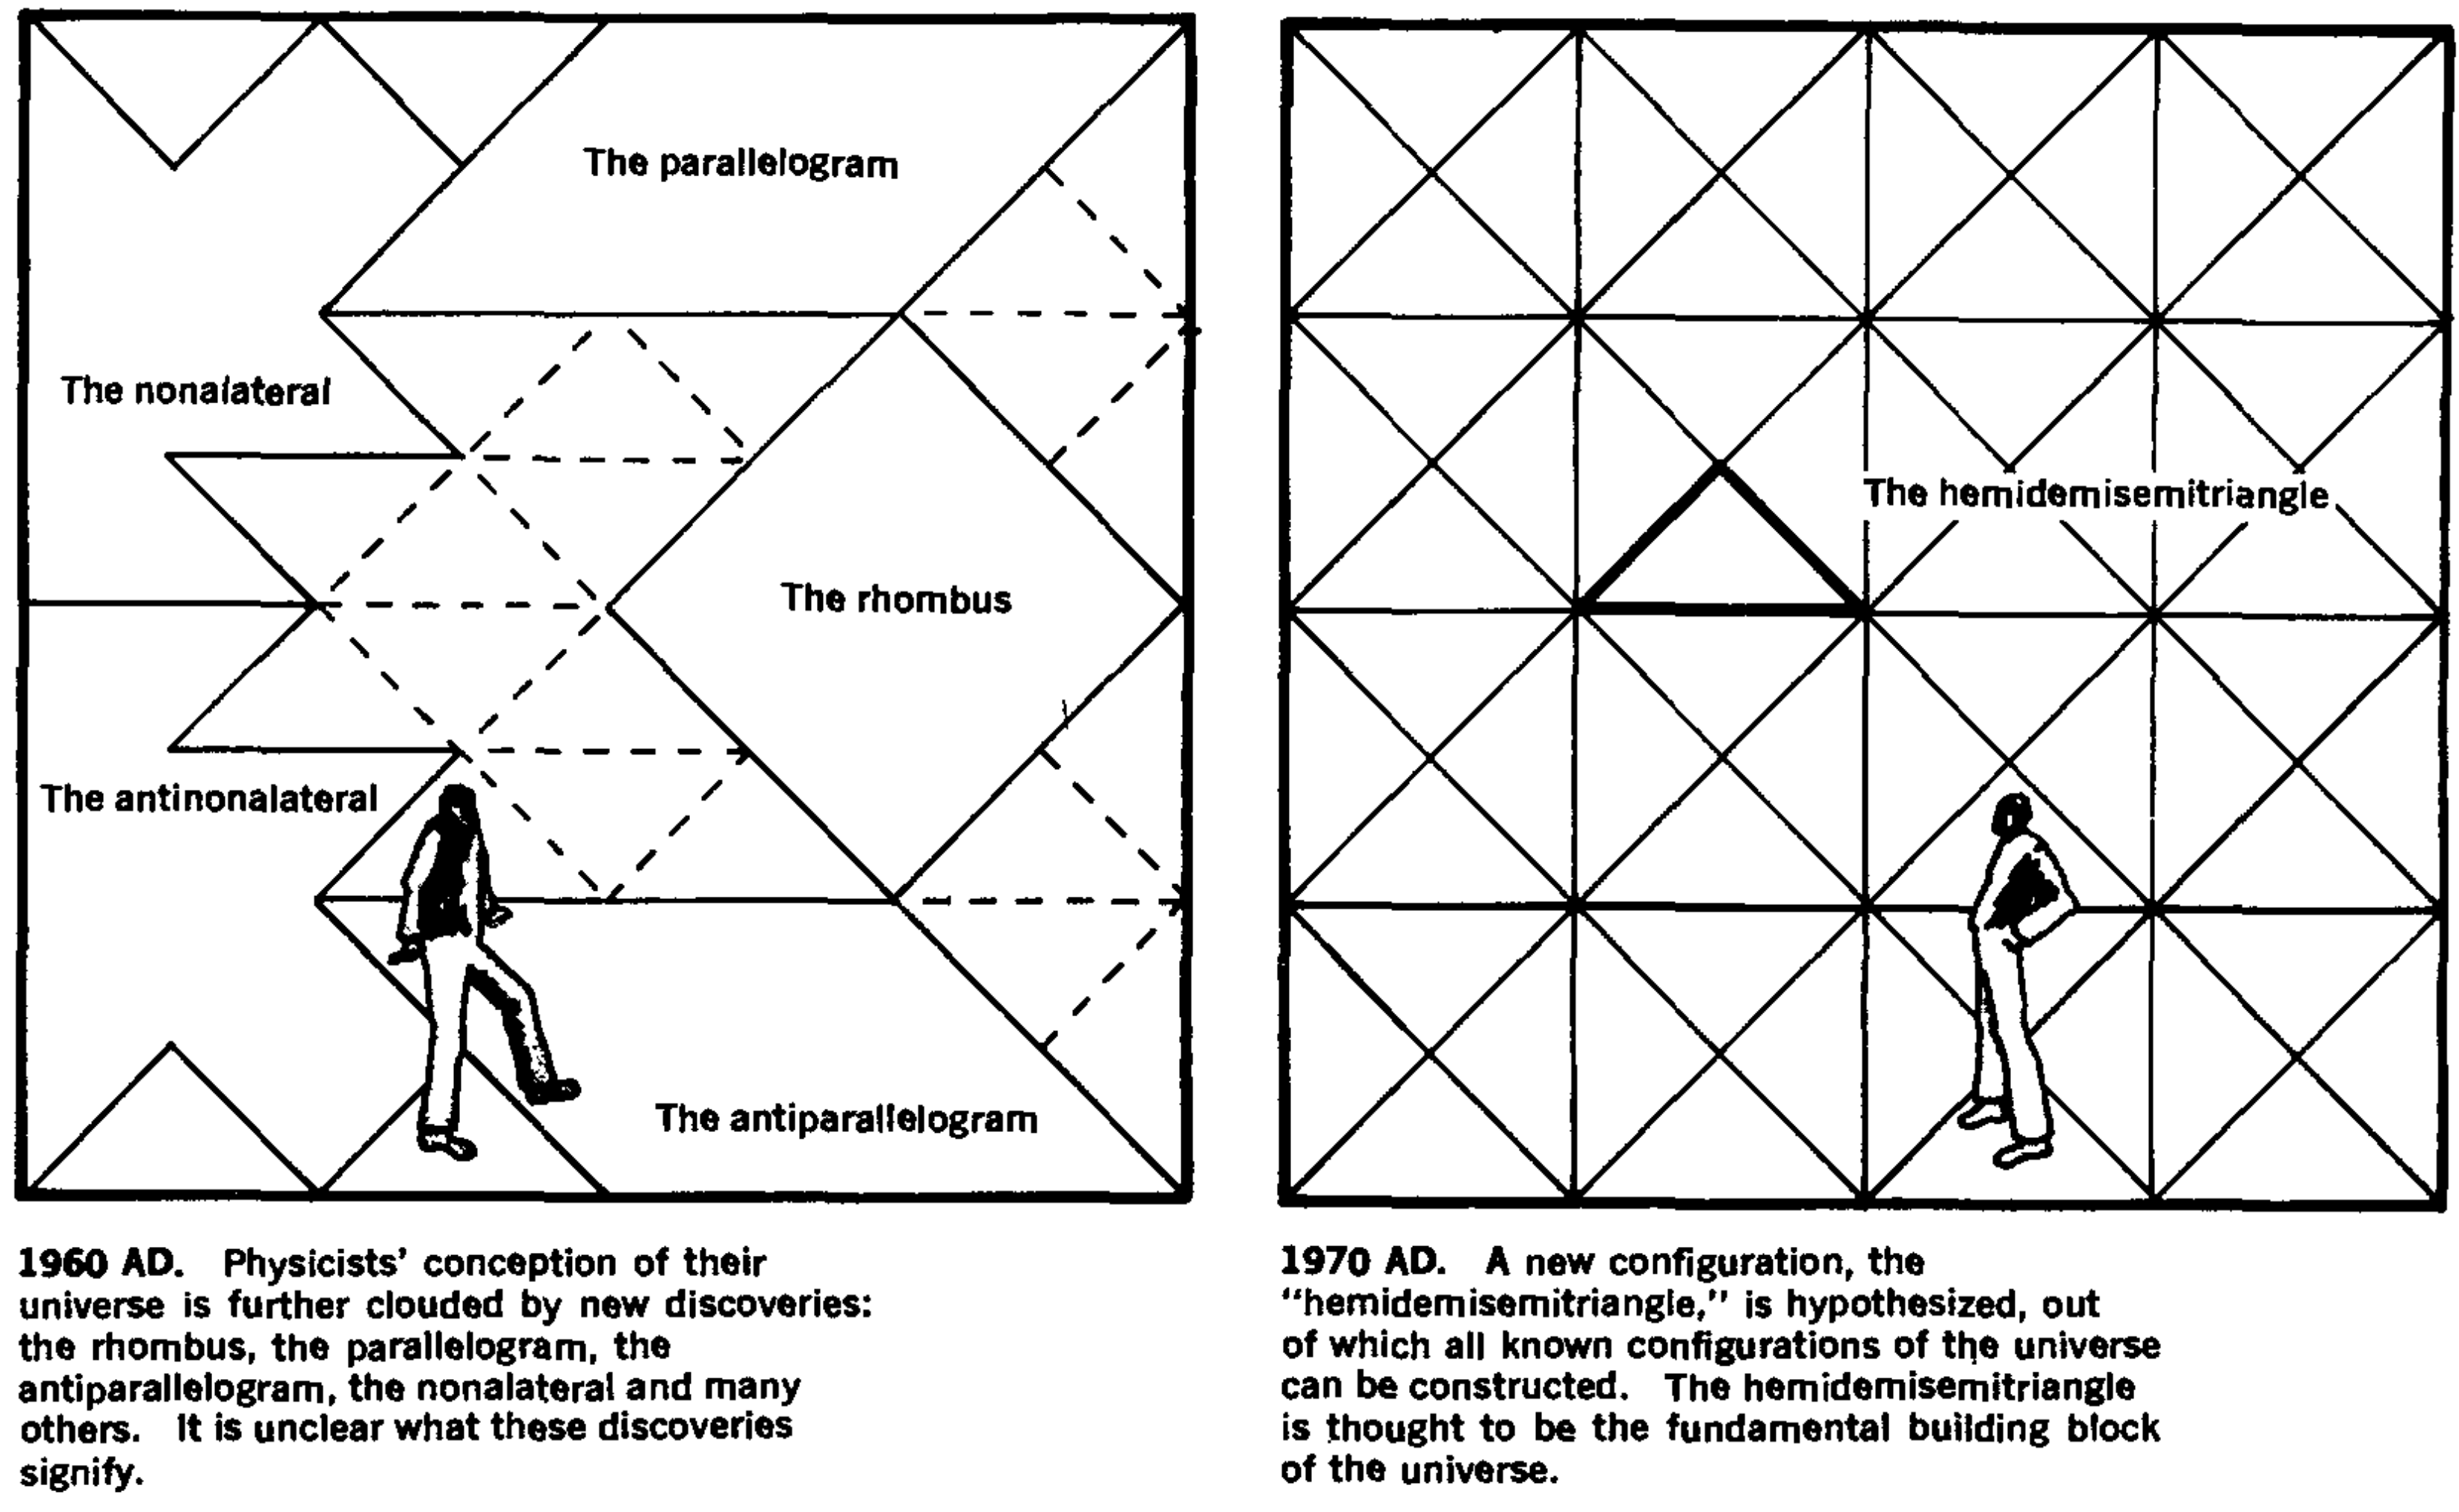
\includegraphics[width=1.2\linewidth]{images/chew3.png}
\\[1em]  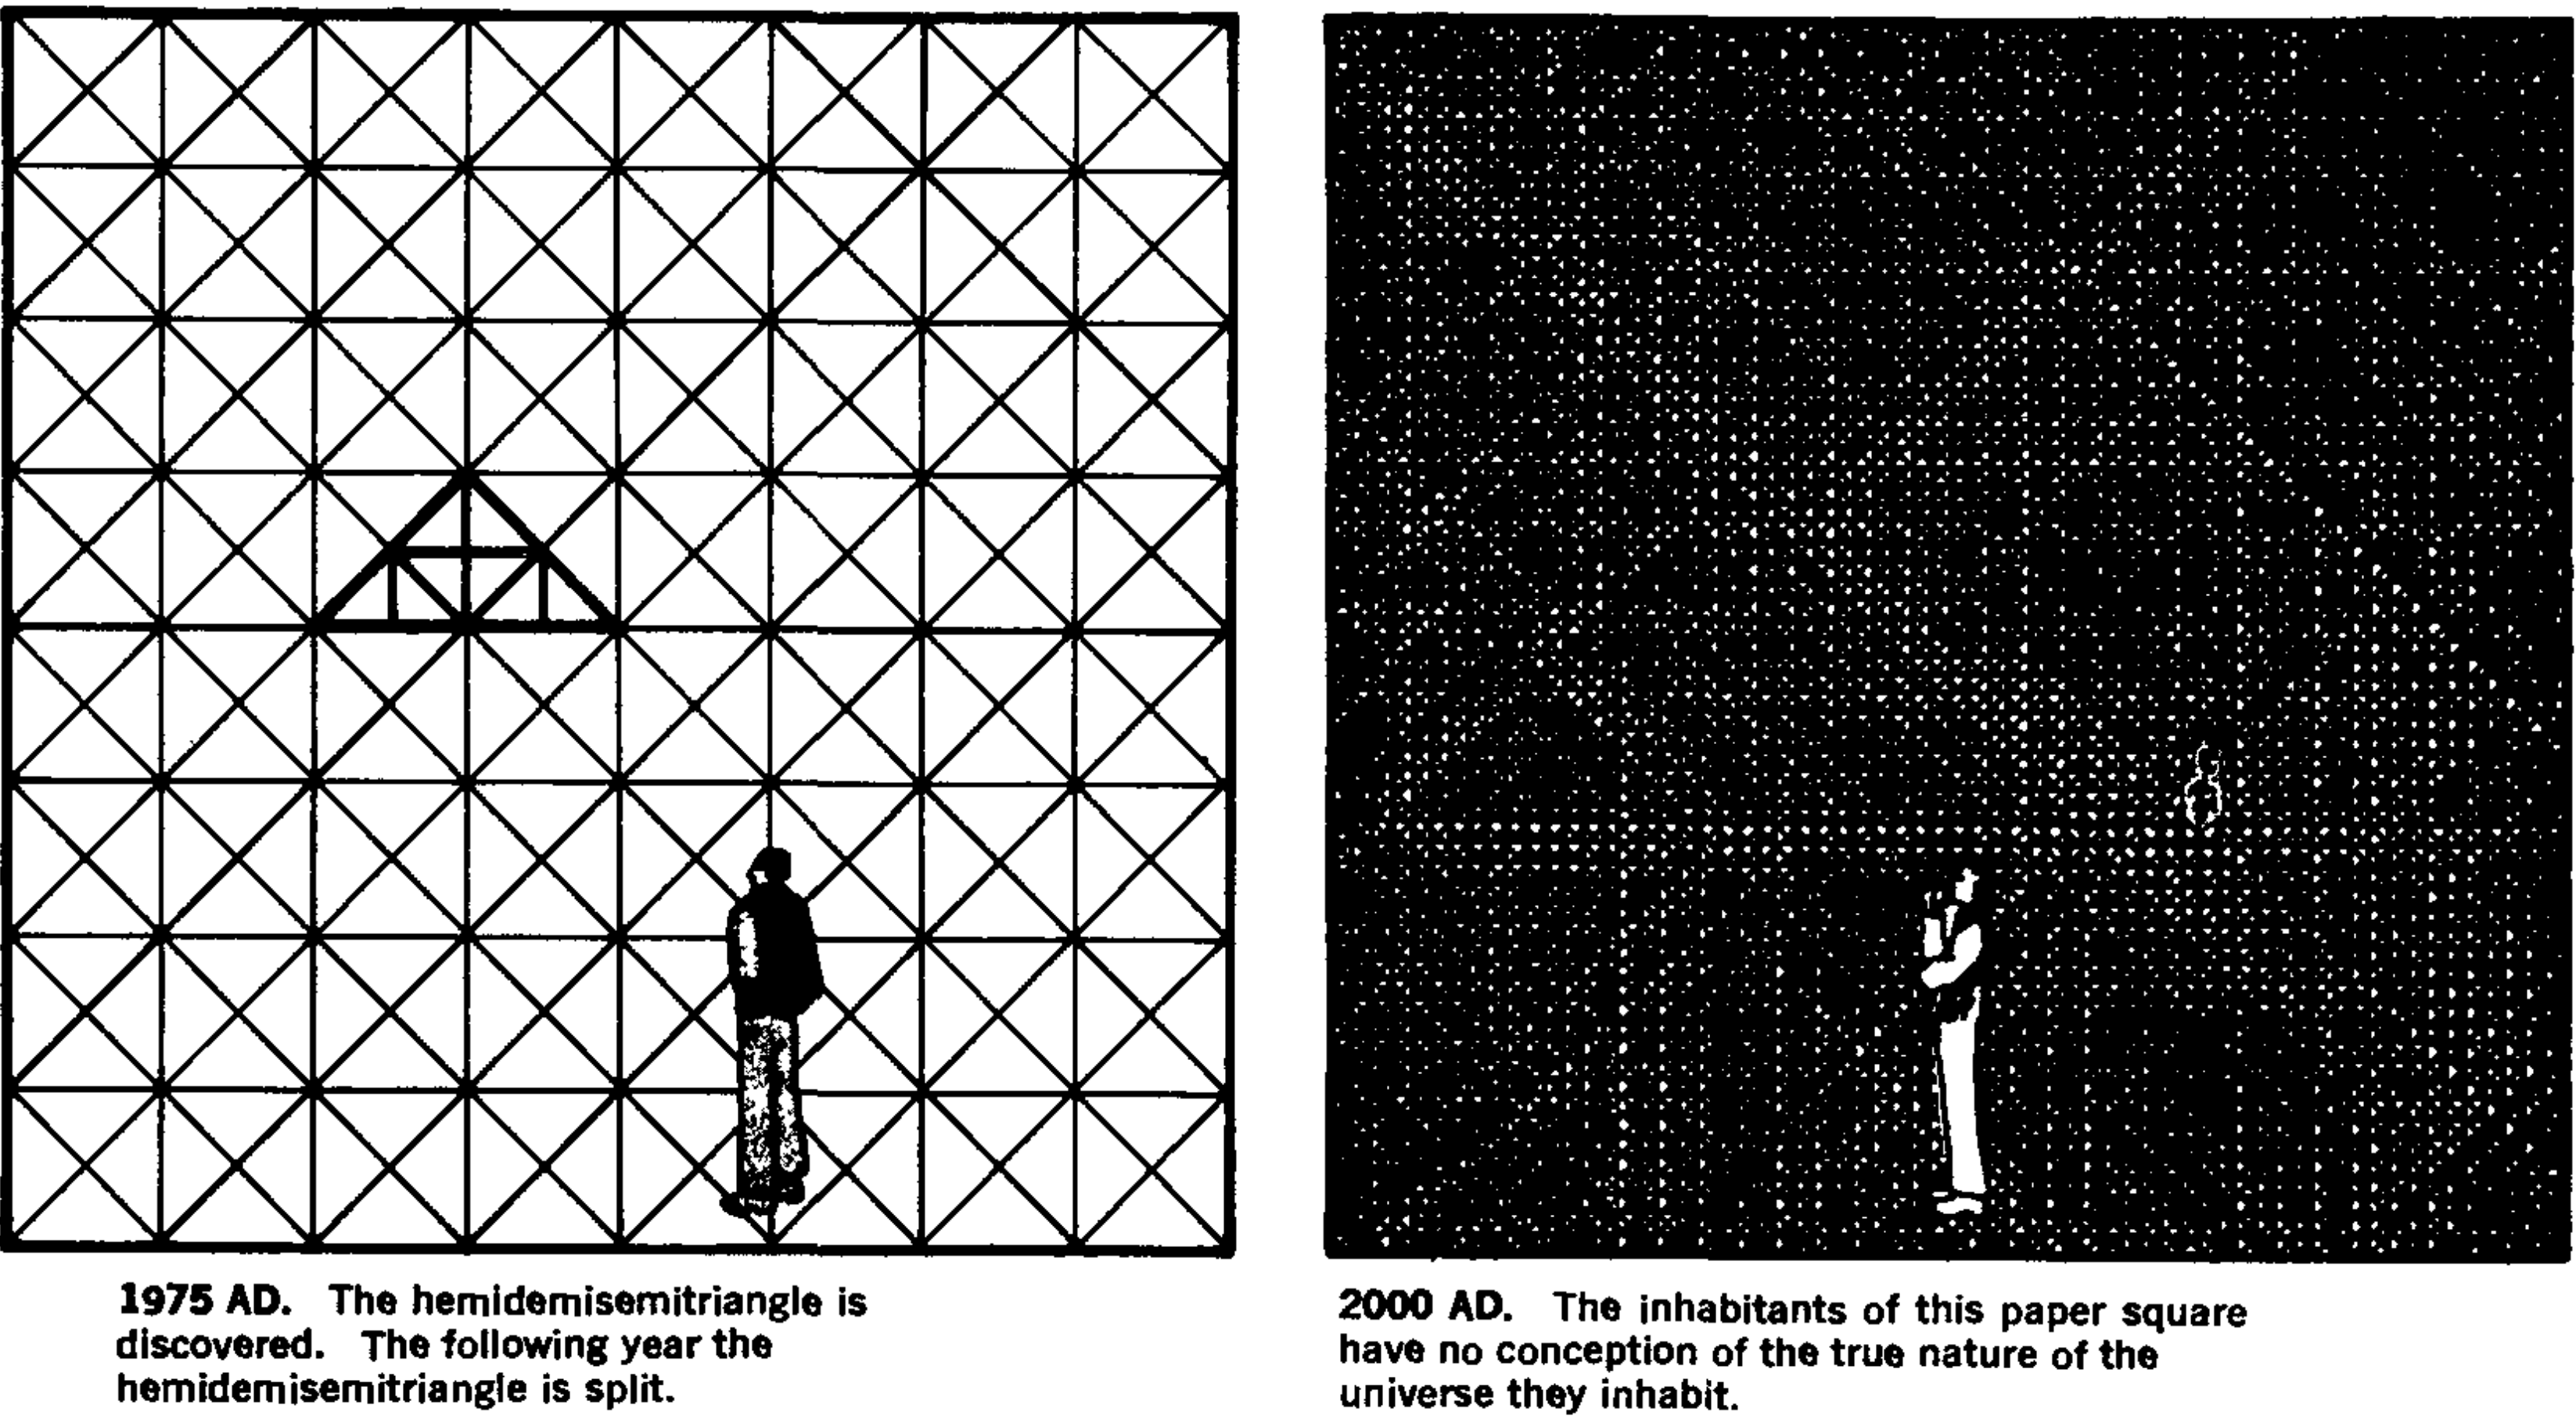
\includegraphics[width=1.2\linewidth]{images/chew4.png}
  % \caption{\emph{\enquote{The progress of \enquote*{fundamental} physics, conceived by Berkeley Chew, published in 1970 by his father, Professor Geoffrey F. Chew.}} Reproduced from  \cites{truesdell1984_r1987}}
  \label{fig:chew2}
\end{figure}

\newpage

\section{Physical laws}
\label{sec:phys_laws0}

\subsection{What's a physical law?}

\marginpar{\vspace{\baselineskip}\footnotesize%
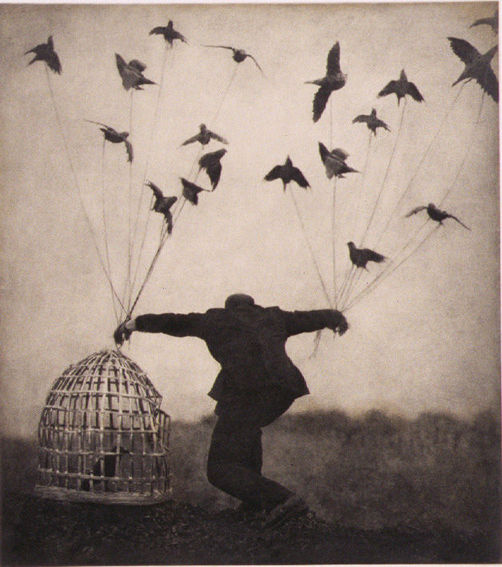
\includegraphics[width=\linewidth]{images/flying_lesson2.jpg}%
\\[\jot]\color{mpcolor}%
Some things, we don't expect to be possible (image: \furl{https://www.parkeharrison.com/bodies-of-work/architect-s-brother/earth-elegies}{\emph{Flying Lesson} by S. \amp\ R. ParkeHarrison}).%
}%
Our lives rely on many kinds of patterns and regular experiences -- so common that we take them for granted and don't even think about them most of the time. If you leave an object in your room in the morning, say a book or a pair of keys, and go out, then when you come back you expect the object to be exactly were you saw it, if you know that nobody entered your room in the meantime. While you go on the street you don't expect to suddenly levitate or flay away. While you write on your notepad, you're not afraid that it might suddenly disappear into thin air. The way we use everyday devices of all kinds relies on predictable behaviours and responses on their part.

All these patterns are regular behaviours that we observe and use are the essential core of physical laws.

A \textbf{physical law}, in the more technical meaning of this term, goes beyond the simple observation or use of such experiences in at least two ways:

First, a physical law goes from qualitative to \textbf{quantitative} observations and expressions. Instead of saying \enquote{the book is still on the table, where I left it}, it might state \enquote{the mass-centre of the book was at position\enskip$(x,y,z)=(0.6,3.1,1.2)\,\unit{m}$\enskip at times $\yti = \text{07:50:31}$ and $\ytf = \text{17:14:40}$}. The use of numbers allow us to convey information in a concise and precise way. Imagine you have to tell someone, who doesn't know Bergen, where in Bergen you are right now, to within \qty{10}{m}. You can do that with a description: \enquote{\textellipsis\ and there's a building called so-and-so which looks like so-and-so\textellipsis}, which would be lengthy and tricky. Or you can just give two numbers: latitude and longitude
\begin{equation*}
  \num{60.36940},\ \num{5.3518} \ .
\end{equation*}
And in these two numbers all digits are important; for instance, the latitude is not \ensuremath{60.369\,4\bm{7}}. The use of mathematics leads to amazing precision and predictive powers. It is this precision, which increases every day, that allows for the operation of technologies so important in our everyday lives: from mobile phones to aeroplanes, from laptops to cars.
%
\marginpar{\vspace{-7\baselineskip}\footnotesize%
\color{mpcolor}\enquote{\emph{There is nothing that can be said by mathematical symbols and relations which cannot also be said by words. The converse, however, is false. Much that can be and is said by words cannot successfully be put into equations, because it is nonsense.}}\sourceatright{\cites{truesdell1966}}
}%

Second, a physical law goes from very specific experiences to more \textbf{general} patterns, which may encompass seemingly very diverse phenomena. Instead of saying \enquote{this book is still here} it might say \enquote{this kind of matter is conserved in any volume and for any amount of time}. Instead of seeing the falling of an apple and the reciprocal movement of planets and sun as two different kinds of phenomena, it summarizes both together as examples of only one physical phenomenon. This generalization leads to the recognition and understanding of many new patterns.

\medskip

In being more quantitative and general, physical laws often become more \textbf{abstract} than everyday observations. Objects like a book and a body of water get included into the more abstract notion of \enquote*{matter}. The movement of different kinds of objects and the propagation of light get included into the more abstract notion of \enquote*{momentum}.

To study and use physical laws we must therefore become familiar with and proficient in seeing and describing physical situations in a more abstract way, and to translate them into mathematical terms. This is what we shall learn in the next \chaps~\ref{cha:time_space}, \ref{cha:stuff}, \ref{cha:contents_fluxes}, so that in \chap~\ref{cha:laws} we shall finally learn and start to use physical laws.


\subsection{Many different mathematical formalisms}
\label{sec:languages}

The mathematics used to express physical laws can come in wildly diverse forms, using wildly diverse principles. This leads to what we may call \enquote{different physics languages}; a more technical name is \enquote{physics formalisms}. One may approach a physics phenomenon or problem in terms of \emph{Lagrangeans}, or \emph{Hamiltonians}, or \emph{fibre bundles}, or \emph{categories}, or \emph{action principles}, or many other formalisms.
\marginpar{\normalsize%
  \begin{gather*}
    \color{red}\delt\!\!\int\!\!L\,\dt = 0 \quad L=\frac12 m v^{2}
    \\
    \color{cyan}\bm{F}=\frac{\di}{\dt}m\bm{v} \quad \bm{F}=0
  \end{gather*}
%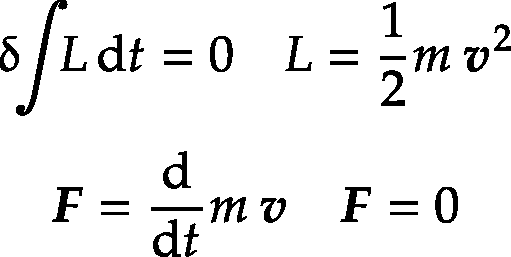
\includegraphics[align=t,width=\linewidth]{images/eg_languages.png}
\footnotesize\color{mpcolor}%
Example of two different formalisms (\textcolor{red}{red}, \textcolor{cyan}{blue}) expressing the same physical phenomenon.%
}
These formalisms or languages are not completely separated; we know how to translate among them. In \enquote{doing} physics, we may jump among formalisms, because some physical situations may be easier to express, or some results easier to find, in one formalism than another. No matter which physics formalism you choose, the results and the concrete applications are still the same. The choice is to a great extent subjective, based on your aesthetic tastes. In \enquote{doing} physics you can actually express your personality and put your own artistic touch; this is why it's such a cool subject; and other scientific subjects are like this too.

In these notes I choose one particular formalism: the one that for me is the most easily \emph{visualizable}; because I believe that visualization can be beneficial in learning new things. Or maybe I choose it just because I like it best. I encourage you to explore how the physics you've learned is expressed in other physics formalisms; maybe you'll like another physics formalism better.

The formalism we'll use might be called \enquote{field theory}. Roughly speaking it takes as starting point the ideas of space and time, or better spacetime, in which there are different kinds of \enquote{stuff}. It expresses the regularity and patterns that we observe in physical phenomena as \enquote{budgets} about the different kinds of stuff, and as relations between them. Please don't take the description just given too literally; it's just meant to give you a very vague idea of the field-theoretical viewpoint.

% \marginpar{\footnotesize%
% \color{mpcolor}\enquote{\emph{this grand book, the universe, which stands continually open to our gaze. But the book cannot be understood unless one first learns to comprehend the language and read the
% letters in which it is composed. It is written in the language of
% mathematics}}\sourceatright{\cites{galilei1623}}
% }


\section{Physical quantities}
\label{sec:primitives}

\subsection{Generalities; scalar and vector quantities}
\label{sec:quants_scalar_vector}

As discussed in the previous section, in order to formulate and use physical laws we need to view all physical phenomena in and around us from a more abstract point of view, which more easily lends itself to quantification. This is done by using the concept of \textbf{physical quantity}.

The \furl{Joint Committee for Guides in Metrology (JCGM)}{Joint Committee for Guides in Metrology (JCGM)} defines \enquote*{quantity} \furl{https://jcgm.bipm.org/vim/en/1.1.html}{as follows}:
\begin{quote}
  property of a phenomenon, body, or substance, where the property has a magnitude that can be expressed by means of a number and a reference.
\end{quote}
As you see it's a somewhat vague definition, but it clearly refers to the possibility of quantification. Some physical quantities are connected with familiar concepts that we use every day, like time, position, distance, velocity, temperature, \energym\ -- but we must be careful because their use in physics is more rigorous and often has technical features that the everyday familiar use has not. Other physical quantities, like momentum, magnetic flux, entropy, are more abstract and disconnected with everyday concepts. Their intuition and use therefore require practice and carefulness.

As stated in the definition above, all physical quantities are expressed as a number together with a \emph{reference}, also called a \textbf{unit of measurement} or simply \emph{unit}. The unit is a basic standard for comparing the measurement of a quantity. For example, when we say that a table has a \emph{length} of two metres, written \enquote*{\qty{2}{m}}, we mean that is it as long as two of those standard lengths that we call \enquote*{metre}. We shall further discuss units of measurement in \sect\,\ref{sec:units}. The number and unit together are handled by usual mathematical rules; so we can for example add or multiply physical quantities. Not all mathematical operations are allowed on all quantities, though.

\medskip

Some physical quantities can be specified by giving only one number together with a unit. Such a quantity is called a \textbf{scalar}. Other physical quantities instead require the specification of several numbers, usually three, with associated units. Such a quantity is called a \textbf{vector}, and can be graphically represented by a vector. There are also quantities that must be specified by several numbers and units, collected together into a sort of matrix. Such a quantity is called a \textbf{tensor}.
\begin{warning}[What's scalar or vector or tensor depends on the theory]
  \emph{Scalar}, \emph{vector}, \emph{tensor} have specific and slightly different meanings in different theories. It is therefore important that you don't take the classification used in these notes as universal.

  \smallskip

  For example, in these notes and in Newtonian mechanics we call \emph{energy density} a scalar, but in General Relativity it isn't a scalar: it is one component of a vector, or even of a tensor.
\end{warning}


\subsection{Derived and primitive quantities}
\label{sec:derived_primitive_quant}

We must briefly discuss a way of categorizing physical quantities which is important for understanding our approach to study physical laws. It's the distinction between \emph{derived} and \emph{primitive} quantities. This is an arbitrary distinction; that is, we can decide, within some bounds, which quantities we consider as \enquote*{derived} and which as \enquote*{primitive}.

A \textbf{derived quantity} is one that we decide to define in terms of other quantities. For example, we can define \emph{speed} $v$ (more precisely: average speed) as the ratio between a \emph{distance} $d$ and a \emph{time duration} $t$:
\begin{equation*}
  v \defd \frac{d}{t}
\end{equation*}
where the symbol \enquote{$\defd$} means \enquote{is defined as} or \enquote{is defined by}. Note how we are already treating and representing \enquote*{speed}, \enquote*{distance}, \enquote*{time duration} as mathematical objects, and doing mathematical operations on them.

Treating \emph{speed} as a derived quantity means that we could in principle avoid using the word \enquote*{speed} and the symbol \enquote*{$v$} altogether, and instead always speak about \enquote*{distance} and \enquote*{duration}, always using the symbols \enquote*{$d$} and \enquote*{$t$} in the combination \enquote*{$d/v$}, instead of using $v$. Doing so would probably lead to very long sentences and formulae, and therefore be extremely inconvenient; but in principle it could be done. The definition of a derived quantity often tells us how that quantity can be measured.

A derived quantity is defined in terms of other quantities, and these may in turn be derived quantities, defined in terms of still other quantities, and so on. But at some point this chain of definitions must come to an end, otherwise we would go around in circles.
\marginpar{\vspace{-3\baselineskip}\footnotesize%
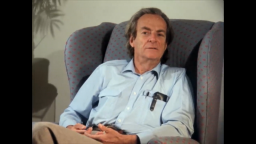
\includegraphics[width=\linewidth]{images/feynman_why2.png}%
\\[\jot]\color{mpcolor}%
\emph{\enquote{you have to be in some framework that you allow something to be true. Otherwise you're perpetually asking \enquote*{why}}.} (\furl{https://www.youtube.com/watch?v=nYg6jzotiAc&t=893s}{see video}).%
}%
A \textbf{primitive quantity} is one that we decide \emph{not} to define in terms of other quantities. That it is not defined in terms of other quantities doesn't mean that we cannot try to explain it. But such explanation must be taken as informal and heuristic. Primitive quantities are often explained through metaphors or by appealing to intuition; but you must always be a little wary of such explanations, because they may fail you spectacularly in some situations. Primitive quantities are the building blocks from which we define all other quantities.

We have therefore a choice about which quantities to take as primitive and which to take as derived. For instance we can define \emph{energy} in terms of quantities like \emph{work} and \emph{heat}, which in turn need to be defined in terms of others, or to be taken as primitive. Or we can take \emph{energy} as primitive, and define \emph{work} and \emph{heat} in terms of it and of other quantities. The latter choice can be more convenient for stating a physical law and for developing a physical theory. It often happens that a quantity, if taken as primitive, is very convenient for building a theory, but difficult to understand intuitively. Vice versa, a quantity can be very intuitive, and therefore convenient as a primitive; but it leads to a complicated theory. We also have some choice in deciding \emph{how many} quantities to take as primitive. Taking as few as possible primitive quantities can actually make the development of a physical theory more difficult, requiring very complicated definitions of the derived quantities.

\medskip

In our study of physical laws we shall take these quantities as primitive:
\begin{center}\bfseries
  time \\ space \\[2\jot] matter \\ electric charge \\ magnetic flux \\ energy-mass \\ momentum \\ angular momentum \\ entropy
\end{center}

\emph{Time} and \emph{space} are taken as primitive quantities -- for obvious reasons -- in almost all current physical theories. We shall discuss them in \chap~\ref{cha:time_space}. The other seven physical quantities, which we shall discuss in \chap~\ref{cha:stuff}, are chosen because of several advantages:
\begin{itemize}[label={\small\faIcon{check}}]
\item They can be understood physically, and treated mathematically, in a similar way. Therefore as we get familiar in thinking about and handling any one of them, we automatically get also familiar with all the others.
\item The way in which they can be understood and handled is intuitive and lends itself to mental visualization.
\item They lead to physical laws that have an almost identical expression. And, as mentioned before, this expression represent a sort of \enquote{budget} and is therefore intuitive.
\item These laws are common to all our physical theories, and they can be expressed in a mathematical form that's the same in any theory.
\end{itemize}
The price to pay for the advantages above is that some of these quantities may be less familiar than others; but the advantages seem to outweigh this disadvantage.

\medskip

We shall also use other quantities, some of which are very familiar, like \emph{temperature} or \emph{pressure}. But the quantities listed above are our fundamental building blocks.


 \section{Physical dimensions and units}
\label{sec:units}

\textbf{Measurement} is the process by which we determine the value of a physical quantity. Measurements can be extremely complex, and can extremely different even if they are about the same quantity. Consider the ways we can measure the \masse\ of a football, compared to the ways we can measure the \masse\ of the Sun.

To each quantity we associate a \textbf{physical dimension}. The term \enquote*{dimension} here has nothing to do with physical extension, as in \enquote{the dimensions of this box}; be careful not to confuse the two. Usually it's clear which one is meant from the context.

Physical dimensions reflect the mathematical relationships that exist between physical quantities. For instance, we take \emph{distance} to have dimension \textsc{length}, and \emph{time interval} to have dimension \textsc{time}; if we now define \emph{speed} as \emph{distance} divided by a \emph{time interval}, then the physical dimension of \emph{speed} is \textsc{length}$/$\textsc{time}. Physical dimensions help us to avoid doing mathematical operations that don't make sense with some quantities. For example, it doesn't make sense to sum up the volume of a glass of water with its temperature. The \furl{https://www.nist.gov/pml/special-publication-811}{International System of Units (SI)} represents the physical dimensions of several base quantities by single capital letters; for instance \enquote*{T} stands for  the physical dimension \textsc{time}. In the present notes we use the different, non-standard convention of denoting a physical dimension by \textsc{small caps}, just to avoid ambiguity and confusion with other one-letter symbols.

\medskip

With each physical dimension we can associate a unit of measurement, which as mentioned in \sect\,\ref{sec:primitives} expresses a basic standard for comparing the measurement results for quantities having that physical dimension. Units are very important and must always be written, for several reasons. First, a number without units doesn't tell us anything. If I tell you \enquote{the place is at a distance 100 from here}, you have no idea how far the place is. \enquote{100} what? 100~metres? 100~kilometres? These are completely different distances. Second, units give us useful information about physical quantities and their relationships and measurement. If you see the expression \enquote{\qty{3}{m/s}}, then there's a strong possibility that that's a velocity. If you see the expression \enquote{\qty{5}{J/m^2}}, then you have a hint that it could be measured by measuring an \energym\ and an area, and then dividing them. Third, keeping track of units often allows us to quickly catch errors in solving a physical problem.

% One can choose a basic set of physical dimensions from which to define all others, as well as a set of standard units for these base dimensions. Here we shall follow the
% \furl{https://www.nist.gov/pml/owm/metric-si/si-units}{International System of Units (SI)} (see also \furl{https://www.nist.gov/pml/special-publication-811}{NIST Special Publication 811}).

If a physical quantity is defined in terms of other quantities, then its unit is usually given in terms of the defining quantities. For example, if we define \emph{speed} as \emph{length} divided by \emph{time}, then its unit is \enquote*{metres per second}, \enquote*{\unit{m/s}}. Some combinations of units receive special unit names. For instance, \emph{power} is defined as \energym\ divided by time; its unit is therefore \enquote*{\unit{J/s}} (\enquote*{joules per second}). But this compound unit is usually called \enquote*{watt}, symbol \enquote*{\unit{W}}. In other words, \enquote*{one watt} and \enquote*{one joule per second} are the same:
\begin{equation*}
  \qty{1}{W} \equiv \qty{1}{J/s} \ .
\end{equation*}

The topics of measurement, physical dimensions, and units, which are studied in \emph{metrology} and in \emph{dimensional analysis}, could occupy an entire course by themselves! I assume that you will look in the documents by the SI for more complicated details. We shall speak further about units in the next chapters. The main quantities and units used in the present notes are summarized in table~\ref{tab:units} on page~\pageref{tab:units} and table~\ref{tab:symbols_volint_fluxes} on page~\pageref{tab:symbols_volint_fluxes}.

\begin{warning}[How to pronounce the quotient and the product of units]
  According to the rules of the SI, the quotient of two units is pronounced \enquote*{per} in English; for instance \enquote*{\unit{m/s}} is pronounced \enquote*{metres per second}. The product of two units is simply pronounced by concatenating the names of the units; for instance \enquote*{\unit{N\cdot s}} is pronounced \enquote*{newton seconds}.

  \smallskip

  For other rules about printing and reporting units take a look at the \furl{https://www.nist.gov/pml/special-publication-811/nist-guide-si-check-list-reviewing-manuscripts}{NIST Check List}.

\end{warning}




\section{Mathematics with quantities and units}
\label{sec:variables_units}

\subsection{Variables and functions}
\label{sec:variables}

When a physical quantity is denoted by a symbol or variable, keep in mind that a unit is \enquote{contained} in the symbol, so to speak. For example if the variable $t$ denotes a time, then it includes some time unit, say seconds. This becomes apparent when we write the value of the symbol, for instance \enquote{$t=\qty{120}{s}$}. The unit is not predetermined, but it must correspond to the dimension of that quantity. We could for instance write \enquote{$t=\qty{2}{min}$} instead; the two expressions are completely equivalent.

This fact must be kept in mind when combining symbols. For example, if $d$ is a distance and $t$ is a time, then writing $v=d/t$ tells us that $v$ is a velocity, and it has appropriate units that come from $d$ and $t$, for instance \unit{m/s}.

Units otherwise behave just like \emph{literal constants} for all mathematical purposes, just like the letter \enquote*{$a$} in the expression \enquote*{$a\, x$}. This is why they can be simplified; for instance:
\begin{equation*}
  \qty{3}{mol/s} \cdot \qty{5}{s} =
  \num{3}\:\frac{\unit{mol}}{\mathcolor{red}{\not}\!\unit{s}} \cdot \num{5}\:\mathcolor{red}{\not}\!\unit{s} = \qty{15}{mol} \ .
\end{equation*}

\medskip

Particular care must be taken with trigonometric and exponential functions, like $\sin()$, $\cos()$, $\tan()$, $\exp()$, $\log()$; \textbf{these functions only admit a dimensionless argument} (which for the trigonometric ones corresponds to \emph{radians}). So there cannot be units like \enquote*{\unit{s}} or \enquote*{\unit{m}} within these functions: we must make sure that any units present within cancel out.

This makes sense, because we wouldn't know how to interpret the argument otherwise. Suppose you read \enquote{$\cos(\qty{60}{s})$} somewhere: how much is that? If we say \enquote{just discard the unit}, we would have
\begin{equation*}
  \cos(\qty{60}{s}) \stackrel{?}{=} \cos(60) \approx -0.95
\end{equation*}
but wait: $\qty{60}{s}\equiv\qty{1}{min}$, so we could equivalently write \enquote{$\cos(\qty{1}{min})$}. Then, according to the hypothetical rule \enquote{just discard the unit}, we would have
\begin{equation*}
  \cos(\qty{60}{s}) \equiv \cos(\qty{1}{min})\stackrel{?}{=} \cos(1) \approx +0.54
\end{equation*}
a completely different result!

For this reason an expression like \enquote*{$\cos(t)$}, with $t$ denoting time, doesn't make sense: there's a time unit in the argument of $\cos()$. If we want to express an oscillation with time, we must write instead something like
\begin{equation*}
  \cos\biggl(\frac{t}{T}\biggr)
\end{equation*}
where $T$ is the period of the oscillation, a symbol which also includes a time unit, which simplifies with the one in $t$. If the period of the oscillation is $T=\qty{1}{s}$ then we can also simply write
\begin{equation*}
  \cos(t/\unit{s})
\end{equation*}
This expression is now unambiguous: suppose that $t=\qty{60}{s}\equiv\qty{1}{min}$, then
\begin{equation*}
  \begin{aligned}
    \cos(t/\unit{s})
    &= \cos(\qty{60}{s}/\unit{s}) =\cos(60) \approx -0.95
    \\
    &= \cos(\qty{1}{min}/\unit{s}) =\cos(1\cdot 60\:\mathcolor{red}{\not}\!\unit{s}/\mathcolor{red}{\not}\!\unit{s}\bigr)
=\cos(60) \approx -0.95
  \end{aligned}
\end{equation*}

\medskip

Also remember that \textbf{the results of trigonometric and exponential functions are dimensionless numbers} as well, so an expression like \enquote*{$3\,\cos(\dotso)$} denotes a pure number, with no units. If you want to express that the result is a length, the appropriate units must appear. We can for instance write
\begin{equation*}
  L\,\cos(\dotso)
\end{equation*}
where $L$ is a length, and therefore includes some kind of length unit such as \enquote*{\unit{m}}. If this length is, say, $L=\qty{2}{m}$ we can also simply write
\begin{equation*}
  2\,\cos(\dotso)\,\unit{m}
\end{equation*}

\subsection{Derivatives}
\label{sec:units_derivatives}

When we follow the rules above, all other mathematical operations automatically take care of everything. The derivative, for instance, is calculated in the usual way, treating any visible units as literal constants. Let's see a concrete example. This expression
\begin{equation*}
x(t) = 2\,\cos(t/\unit{s})\,\unit{m}
\end{equation*}
says that the position of some object oscillates with time, between the values \qty{-2}{m} and \qty{+2}{m}. When $t=\qty{0}{s}$, the position is $x=\qty{+2}{m}$. The position $x=\qty{-2}{m}$ is reached when the argument of $\cos()$ is $\pu$, that is
\begin{equation*}
  t/\unit{s} = \pu \quad\limplies\quad t\approx \qty{3.14}{s} \ .
\end{equation*}

The \autoref{sec:velocity}{velocity} of the object is given by the derivative of this expression with respect to $t$. Let's calculate it treating all unit symbols as literal constants:
\begin{equation*}
  \frac{\di x(t)}{\dt} = \frac{\di}{\dt}\Bigl(
  2\,\cos(t/\unit{s})\,\unit{m}
  \Bigr)
  =
  2\,\Bigl[
  \mathcolor{grey}{\underbracket{\color{black}-\sin(t/\unit{s})\cdot\frac{1}{\unit{s}}}_{\zerob{\color{grey}\footnotesize chain rule}}}
  \Bigr]\,\unit{m}
  =
 -2\,\sin(t/\unit{s})\,\unit{m/s}
\end{equation*}
and you see that the correct units for velocity have automatically appeared.



\printpagenotes*
\cleartooddpage
\chapter{Time and space}
\label{cha:time_space}

\epigraph{If we want to describe the \emph{motion} of a material point, we give the values of its coordinates as a function of time. However, we should keep in mind that for such a mathematical description to have physical meaning, we first have to clarify what is to be understood here by \enquote{time}. We have to bear in mind that all our propositions involving time are always propositions about \emph{simultaneous events}. If, for example, I say that \enquote{the train arrives here at 7 o'clock}, that means, more or less, \enquote{the pointing of the small hand of my clock to~7 and the arrival of the train are simultaneous events}.}{A. Einstein \cites*{einstein1905c}}




\section{Time and proper time}
\label{sec:time}

% \subsection{Proper time: what's \enquote{now}?}
% \label{sec:proper_time}


\emph{Time} is a primitive quantity. We understand the notion of time intuitively, even if it is difficult to explain -- that's why it is taken as primitive. In 1905, with the Theory of Relativity, part of our everyday intuition about the notion of time was seriously shaken. For many years afterwards our old intuition could still be used in practice and in applications. But the new, correct intuition is becoming more and more important in everyday life and technologies. GPS navigation, for example -- which we use every day in leisure activities like hiking or sightseeing, as well as in more critical ones like aeroplane landing -- crucially depends on the correct notion, intuition, and measurement of time. Luckily the new intuition of time is also becoming more and more widespread thanks to films and mass-media; think of movies like \furl{https://www.imdb.com/title/tt0816692/}{\emph{Interstellar}}.

Let's see, by means of a thought experiment, how our traditional intuition about time goes astray. Here's Alice, Bob, and Charlie. They have extremely precise clocks, built in exactly the same way. They synchronize their clocks and stay very close to one another. Keeping close, they go around, maybe on an aeroplane or on a space ship, and they constantly compare their three clocks. They notice that their clocks stay perfectly synchronized all the time, no matter where they go and what they do.

At some point they separate, and each one goes around independently. One of them might stay in place, another might take a helicopter, and another might go for a trip to Mars and back.

Alice and Bob at some point meet again, and compare their clocks. They see that their clocks are not synchronized anymore; the difference could be as small as microseconds, or as large as years. In fact, if this time discrepancy is large, they notice that they have also aged differently: the time difference is not only apparent in their clocks, but also in their bodies. Let's say for concreteness that Alice's clock is ahead of Bob's, or equivalently that Bob's clock is behind Alice's. Note the following aspects:

First, both Alice and Bob can say \enquote{my clock has been working fire, so it should be correct}: neither has noticed anything strange about the passage of time.

Second, if they now stay together, they see that their clocks remain exactly synchronized, besides the time discrepancy they noticed when they met again. This discrepancy doesn't increase or decrease. They might even retrace together Alice's and Bob's previous trips; their clocks will still remain synchronized.

Third, they might wonder what the time is on Charlie's clock. But Charlie is at some distance away. They could decide to contact Charlie, say via radio, and ask \enquote{what does your clock show, right \emph{now}?}. But they would notice that there's a delay, even if extremely small, in the radio transmission; so it's unclear to what time Charlie's answer would apply. If we say \enquote{let's account for the radio-signal speed}, we see that there's a logical problem: speed is distance divided by \emph{time}, and here we have a problem in exactly determining what's the \enquote{correct} time! So we would be reasoning in circles. But even neglecting these difficulties, Charlie's answer could reveal a time that is completely different from Alice's and from Bob's -- it could be years ahead or behind both of theirs!

%\calccentering{\unitlength}
\begin{figure}[p]
%\begin{adjustwidth}{\unitlength}{-\unitlength}
  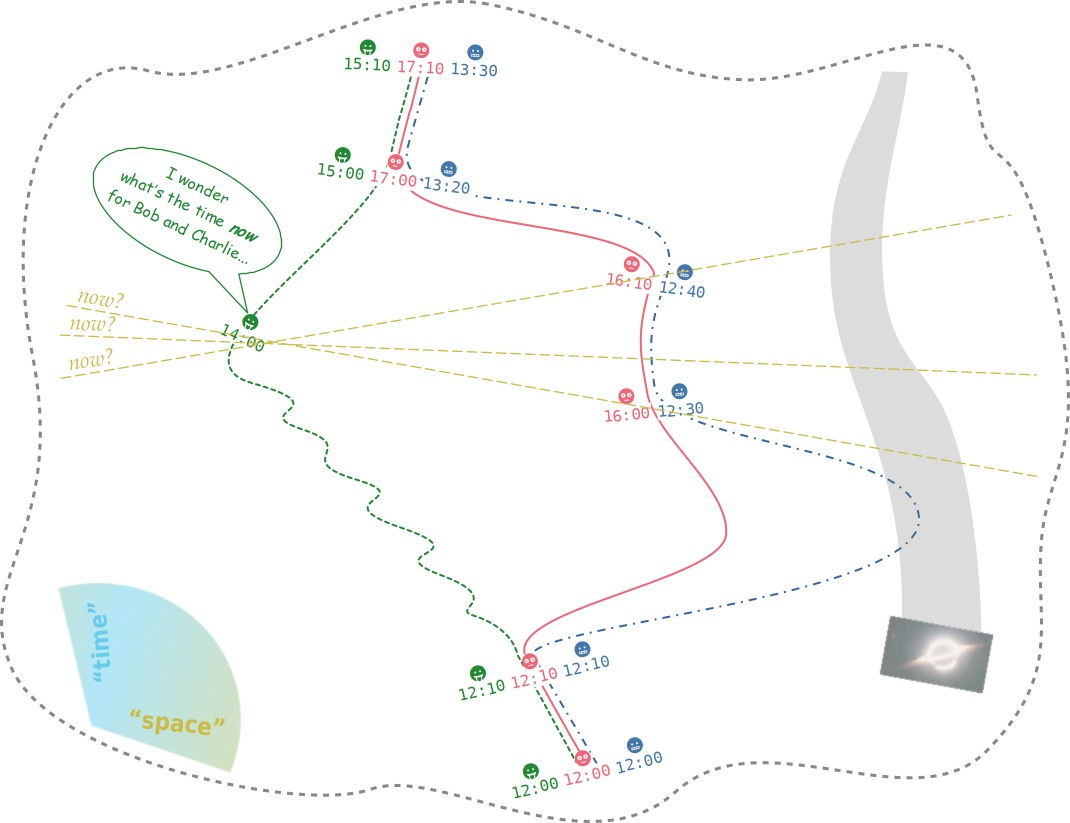
\includegraphics[width=\linewidth]{images/ABC_spacetime.jpg}
  \caption{A \emph{spacetime diagram} that illustrates of the experiences of Alice (\textcolor{green}{dashed \faIcon{grin-tongue}}), Bob (\textcolor{red}{solid \faIcon{flushed}}), Charlie (\textcolor{blue}{dot-dashed \faIcon{grimace}}) with time. The area within the \textcolor{midgrey}{grey dotted line} represents a two-dimensional spacetime. Space is more horizontal than vertical; time is more vertical than horizontal, and flows upward. Note that we can't precisely say, for instance, \enquote{the vertical direction is time}, because our problem is to see whether we can really separate time and space at all.
    %
\\[2\jot]\textbf{Lower part}: Alice, Bob, Charlie stay close and observe their clocks are perfectly synchronized from 12:00 to 12:10. Then they separate.
%
\\[\jot]\textbf{Right}: Charlie visits a region near a strong \masse\ source. Upon meeting again with Bob, the two notice their clocks differ: 16:00 for Bob, 12:30 for Charlie. Yet this clock difference stays the same while they travel together for \qty{10}{min}.
%
\\[\jot]\textbf{Left}: Alice wanders around, travelling at high speed with respect to the fixed stars. When her clock displays 16:00, she wonders what's the time \enquote{right now} for Bob and Charlie. But this question doesn't make sense, because
(1)~when Bob and Charlie are together their clocks differ -- impossible to say what's \enquote{the} time at their position; (2)~it is not clear which instant in Bob \amp\ Charlie's trajectory should be considered as \enquote{now} for Alice (\textcolor{yellow}{yellow dashed lines}).
%
\\[\jot]\textbf{Upper part}: When Alice, Bob, Charlie meet again, their clocks have completely different readings; and they have aged differently. But their clocks run again at the same rate as long as they stay close again.}  \label{fig:ABC_spacetime}
%\end{adjustwidth}
\end{figure}
%\clearpage

The experience just described will occur again any time Alice, Bob, Charlie, or any two of them, meet. There could be a hundred observers like Alice, Bob, Charlie, initially at the same place and with synchronized clocks. Whenever two or more of them meet after having been separated, they will notice discrepancies in their clocks (and in the ageing of their bodies). But their clocks will have exactly the same time lapses as long as they stay together.

%
\marginpar{\vspace{-\baselineskip}\footnotesize\centering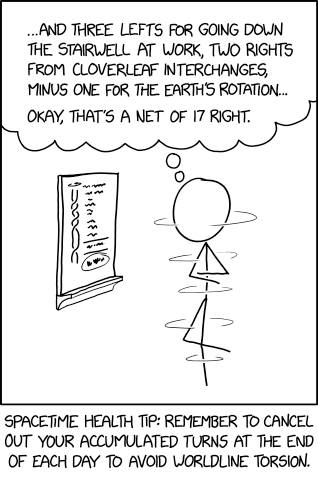
\includegraphics[width=\linewidth]{images/net_rotations.png}\\[-\jot]\color{mpcolor}\url{https://xkcd.com/2882}%
}%
This situation is illustrated in \fig~\ref{fig:ABC_spacetime}, which is an example of \textbf{spacetime diagram}. The figure represents the temporal dimension and one spatial dimension merged together in a two-dimensional image. The motions of Alice, Bob, Charlie \enquote*{in space} are therefore represented as lines in this two-dimensional spacetime. They are called \emph{worldlines}. Each point in a worldline has an associated time, the time measured by the person or object following that worldline.

\medskip

Consider for a moment an imaginary world in which these experiments had given a different kind of result. According to Newtonian mechanics, whenever two or more initially synchronized observers like Alice, Bob, Charlie were to meet again, their clocks would always show identical times. If one year, 23 days, 8 hours, 9 minutes, and \num{3.04539928324099266302} seconds had passed for Bob since he last met Alice, he would see that exactly the same amount of time had passed for Alice since their previous meeting. If you think about it, in this case it would have beeen somewhat natural for them to think \enquote{right now, the clock of far-away Charlie must show the same time as ours} (even though they have no real experimental way of confirming that).
% %
% \marginpar{\vspace{-2\baselineskip}\footnotesize\color{mpcolor}\enquote{\emph{%
% The plot for Cesium \textelp{} characterizes the best orbiting clocks in the GPS system. What this means is that after initializing a Cesium clock, and leaving it alone for a day, it should be correct to within \textelp{} 4~nanoseconds. Relativistic effects are huge compared to this.}}\sourceatright{\cites{ashby2003}}
% }
% %

But that's an imaginary world. In our world what occurs is the more complicated situation with time discrepancies described initially. Only one conclusion can be drawn from these experimental results: \textbf{Time is not some sort of universal quantity. It is, so to speak, \enquote{local} to a person or clock, or to a group of persons or clocks that stick together.} This also means that it does not make sense to ask questions like \enquote{what is the time for far-away Charlie, \emph{right now}?}, or \enquote{what is happening at some other place \emph{right now}?}. There is no universal \enquote*{now}; the notion of \emph{now} is local.


The time measured by a specific observer is called the \textbf{proper time} of that observer. Luckily we know how to calculate how much the proper times of separated observers will differ when the observers meet again. According to our current understanding, it turns out that the time differences depend, roughly speaking, on how fast the observers are moving with respect to one another and with respect to the distribution of \energym\ in the universe, and on how much \energym\ is contained in the regions they travel across. The general theory of relativity gives us the equations that determine the proper-time differences.

% The situation depicted in our initial thought-experiment is real.
Time discrepancies can be measured, for example, by comparing initially synchronized clocks that have been put in aeroplanes flying in different directions. The first measurement of this kind was made by Hafele and Keating in 1971. They synchronized four caesium atomic clocks with a reference clock, and then flew the four atomic clocks around the world on commercial jet flights, first eastward, then westward. At the end of the eastward trip, the clocks showed a time \emph{behind} the reference one by around \qty{6e-8}{s}. At the end of the westward trip, their time was \emph{ahead} the reference one by around \qty{3e-7}{s}. These measurements were in agreement with General Relativity's prediction, within experimental error.
%
\marginpar{\vspace{-8\baselineskip}\footnotesize\centering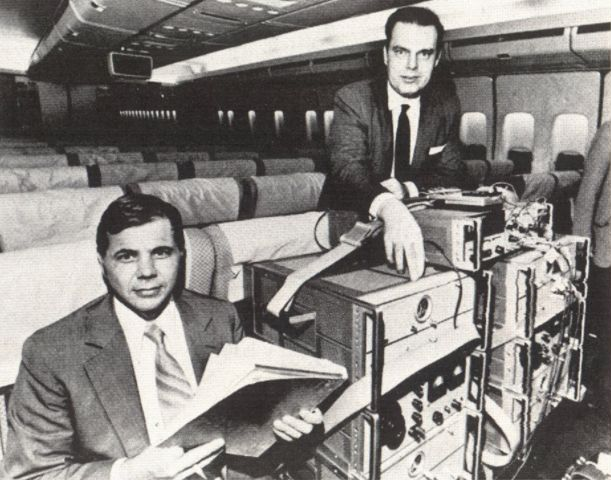
\includegraphics[width=\linewidth]{images/hafele_keating_time.jpg}\\\flushleftright\color{mpcolor}Hafele, Keating, and their clocks aboard aeroplane (from \furl{https://time.com/vault/issue/1971-10-18/page/93}{\emph{Time}, October 1971})%
}%

Most importantly, these time discrepancies affect everyday technologies such as the Global Positioning System. Formulae from General Relativity appear in your phone's GPS software; see for instance \sect\,20.3.3.3.3 of the Interface Control Document \texttt{IS-GPS-200} at \url{https://www.gps.gov/technical/icwg/}. Time discrepancies must also be taken into account in the establishment and synchronization of time in our everyday equipment:
\begin{quote}\footnotesize
  In 1976, the International Astronomical Union introduced relativistic concepts of time and the transformations between various time scales and reference systems. \textelp{} Now \textelp{} it is necessary to base all astrometry, reference systems, ephemerides, and observational reduction procedures on consistent relativistic grounds. This means that relativity must be accepted in its entirety, and that concepts, as well as practical problems, must be approached from a relativistic point of view.
  %
  \sourceatright{\parencites{kovalevskyetal2004}}
\end{quote}
%
% \marginpar{\vspace{-6\baselineskip}\footnotesize%
% \color{mpcolor}\enquote{\emph{In 1976, the International Astronomical Union introduced relativistic concepts of time and the transformations between various time scales and reference systems. \textelp{} Now \textelp{} it is necessary to base all astrometry, reference systems, ephemerides, and observational reduction procedures on consistent relativistic grounds. This means that relativity must be accepted in its entirety, and that concepts, as well as practical problems, must be approached from a relativistic point of view.}}\\{\cites{kovalevskyetal2004}}
% }

Note therefore the following curious situation. In setting up a time to meet a friend, you don't need to worry about the discrepancies between your and your friend's proper times: if your friend walks \qty{1000}{m} away from you and then immediately back to you, at \qty{1}{m/s}, then the time elapsed for you will be \qty{1000}{s} (around \qty{17}{min}), but the time elapsed for your friend will be \qty{999.999999999999994437}{s}. That's a difference of less than \qty{e-14}{s}, clearly negligible for the two of you, so you don't need to worry with General Relativity formulae in setting up your meeting time. Yet, if you set up a meeting place via GPS, then the true nature of time and General Relativity formulae become important: if they were not accounted for, you and your friend might end up off your meeting place by \qty{100}{m}.
% In most everyday situations for us, who live on or nearby Earth's surface and move at speeds much smaller than $\yc$ with respect to one another, the discrepancies between our proper times are so small that they cannot be measured with ordinary clocks or with our internal clocks. Consider a person walking \qty{10}{m} away from you and then immediately walking back to you, at \qty{1}{m/s}. The time elapsed for you will be \qty{20}{s}, but for that person will be \qty{19.999999999999999889}{s}, a difference of \qty{e-16}{s}, which is the error of an atomic clock. %%***add ref
% If human beings will still exist in some decades or centuries, in space travel they will have to deal with large proper-time discrepancies also in everyday life.

Time lapse or duration has SI dimension \textsc{time}, and we shall usually measure it using the unit \emph{second}, symbol \enquote*{$\unit{s}$}.

% *** add short explanation of second




\begin{exercise}[label={ex:clocks}]
  Consider two clocks: one at rest on the Earth's surface, at a distance $\color{green}r_{\text{e}}$ from the Earth's centre; the other on a GPS satellite or, say, on the \furl{https://www.nasa.gov/international-space-station/}{International Space Station}, right above the first clock, at a distance $\color{red}r_{\text{s}}$ from the Earth's centre. An observer by the clock on Earth measuring a time lapse $\Dt_{\text{e}}$ will see that the clock on the satellite has run for a time lapse $\Dt_{\text{s}}$. The relation between two time lapses is approximately given by
\sidepar{\centering%
  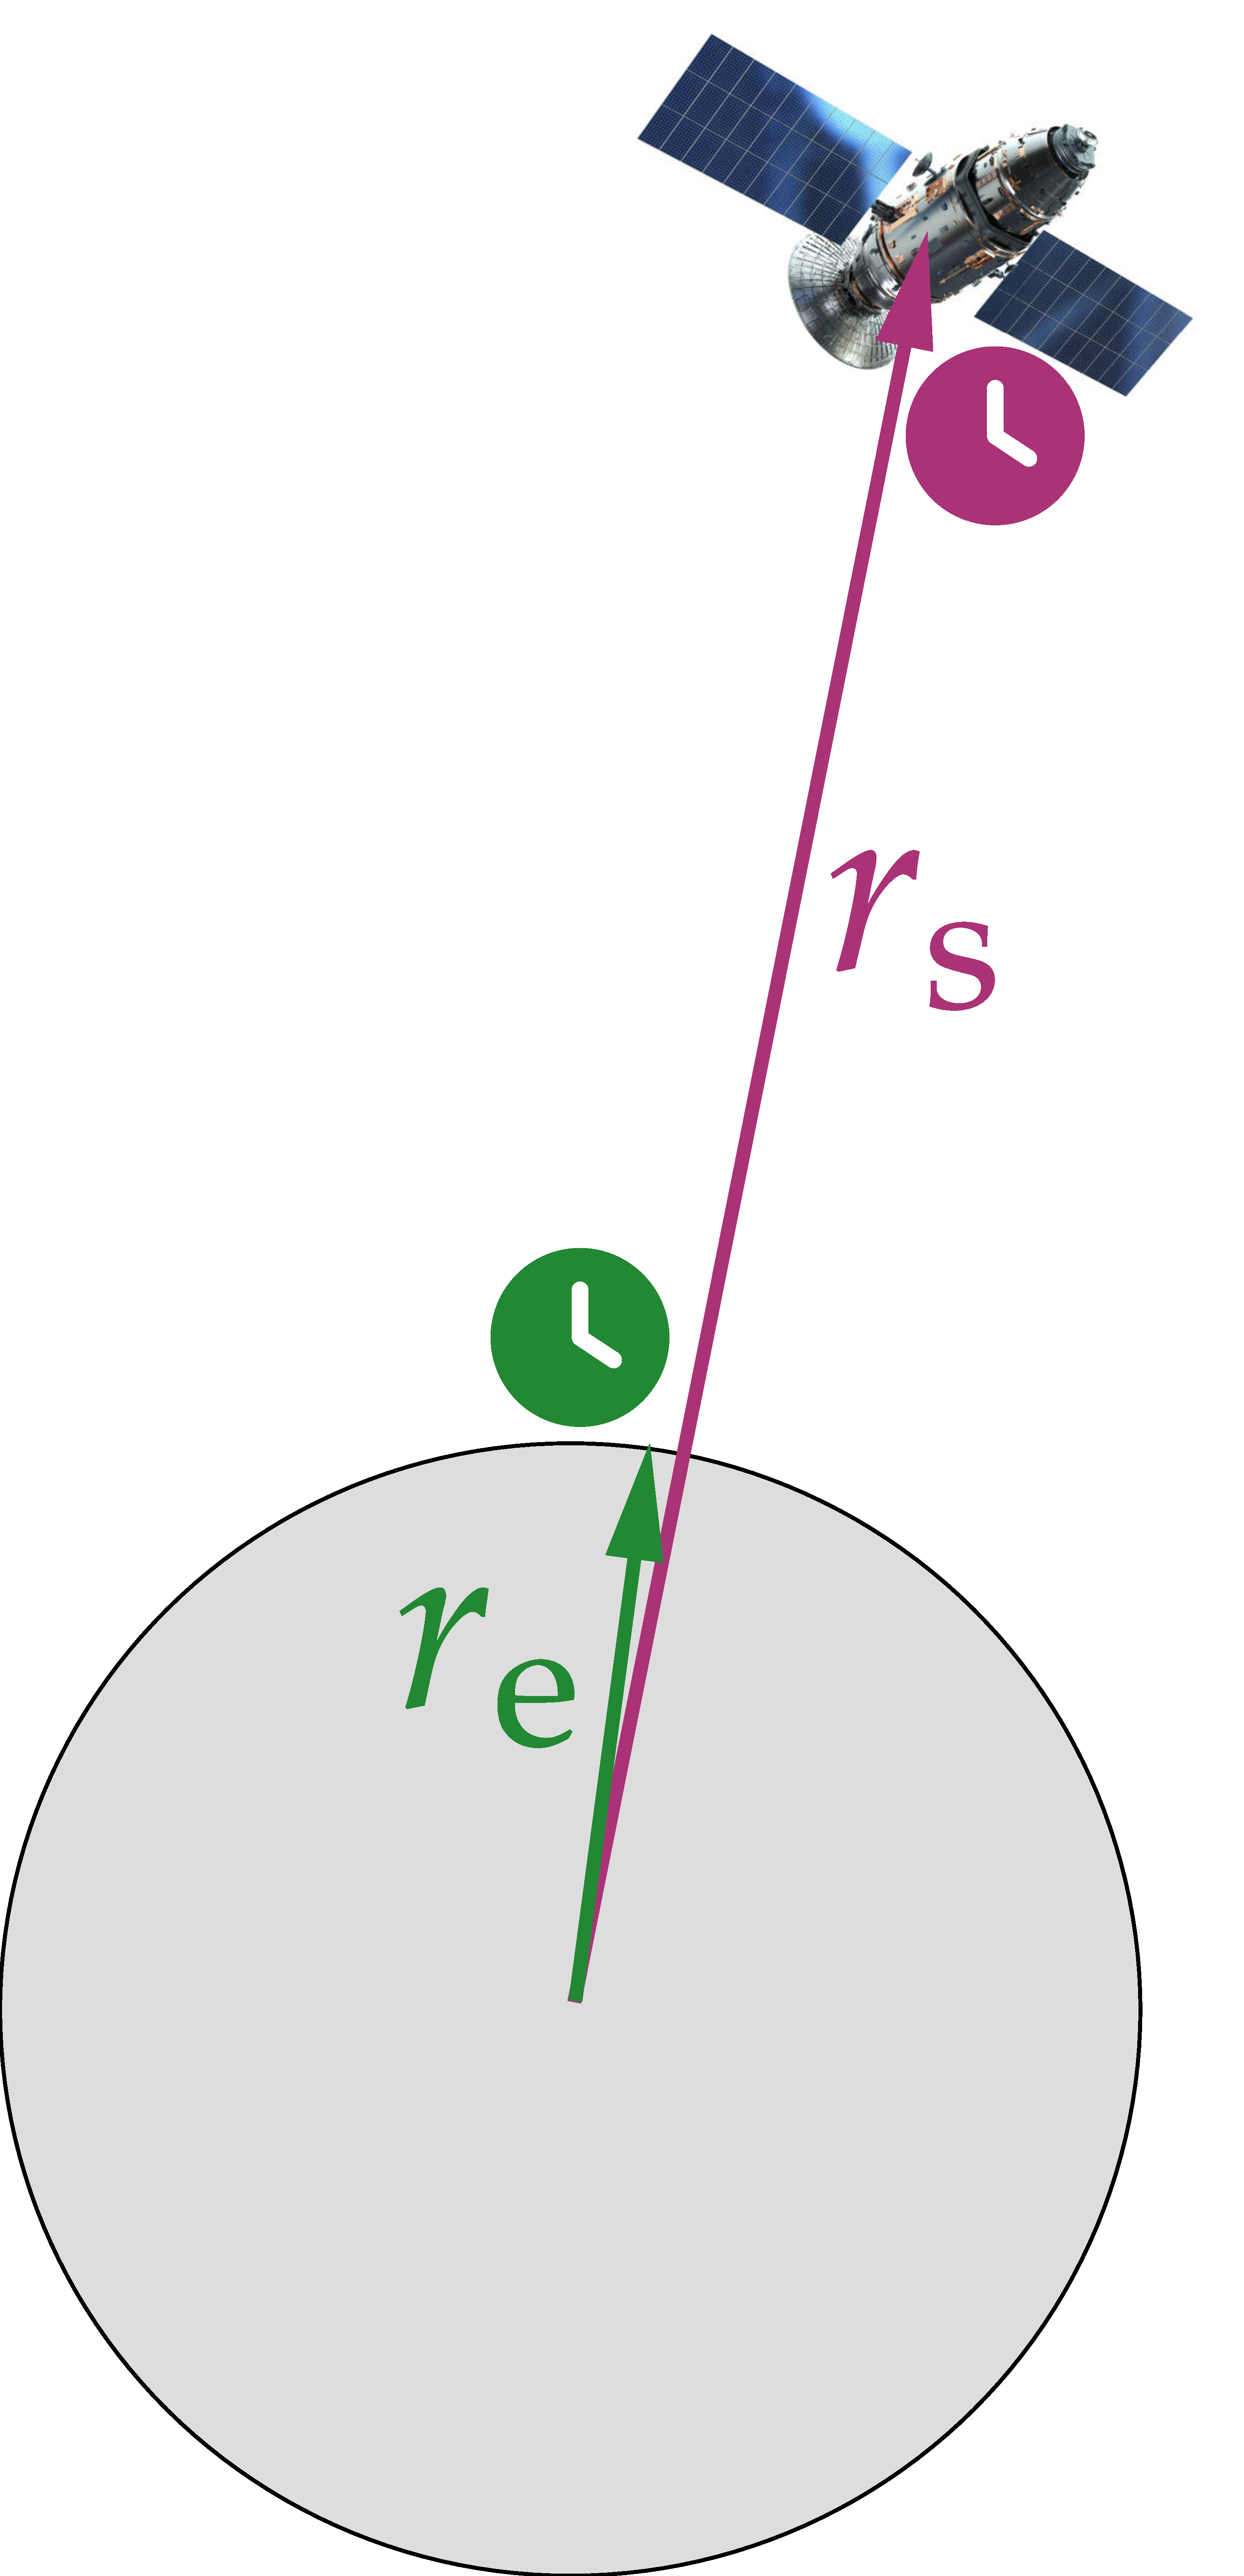
\includegraphics[align=t,width=0.75\linewidth]{images/re_rs.pdf}
}
\begin{equation*}
  \frac{\Dt_{\text{s}}}{\Dt_{\text{e}}} =
  \frac{
    \sqrt{1-2\frac{G}{c^{2}}\frac{M}{r_{s}}}
  }{
    \sqrt{1-2\frac{G}{c^{2}}\frac{M}{r_{e}}}
  }
\end{equation*}
where $G\approx\qty{6.7e-11}{m^{3}/(kg.s^{2})}$, $c=\qty{3.0e8}{m/s}$, and the Earth's \masse\ $M=\qty{6.0e24}{kg}$.

\begin{enumerate}[exerc]
\item\label{item:gps_clock} Take the case of a GPS satellite, with $r_{\text{e}}=\qty{6.4e6}{m}$ and $r_{\text{s}}=\qty{2.6e7}{m}$ (\furl{https://www.nasa.gov/directorates/somd/space-communications-navigation-program/gps/}{NASA data}). If you, on the ground, measure a time lapse of $\Dt_{\text{e}}=\qty{10}{years}$, what's the difference, in seconds, with the time lapse $\Dt_{\text{s}}$ you see on the satellite?

\item\label{item:interstellar} If the time lapses are large compared with the time needed to go from ground to orbit or vice versa, then $\Dt_{\text{s}}/\Dt_{\text{e}}$ is also the ratio between the real \emph{ageing} of a person who's been in orbit and one who's been on the ground, when they meet again.

  Now consider the case with a black hole instead of Earth. The formula above can still be applied as an approximation.

  In the film \furl{https://www.imdb.com/title/tt0816692/}{\emph{Interstellar}}, two
  astronauts travel to Miller's planet, at a distance $r_{\text{e}}$ from the black hole Gargantua, while leaving a third astronaut in orbit at a distance $r_{\text{s}}\approx \infty$ (the distance is large enough that it can be approximated as infinity). The two astronauts stay on Miller's planet for \qty{3}{hours}. When they meet the latter astronaut in orbit again, the latter has aged \emph{23\;years}.
\sidepar{\footnotesize\centering%
\vspace{-7em}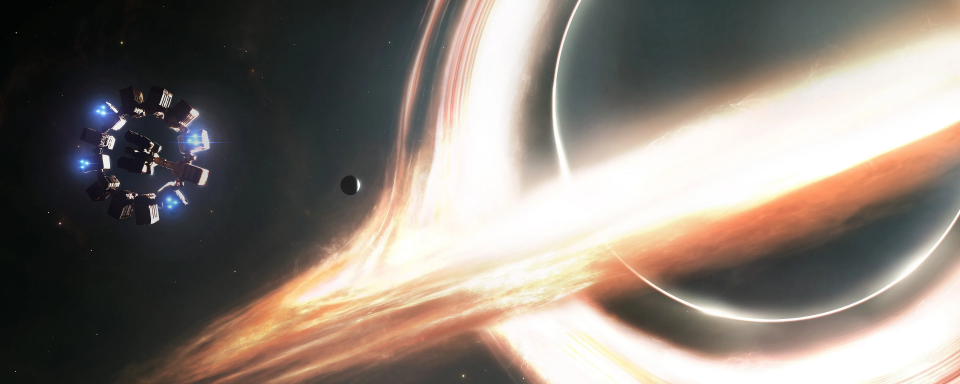
\includegraphics[width=\linewidth]{images/gargantua.png}
}

  Given that Gargantua's \masse\ is $M=\qty{2.0e38}{kg}$, calculate the distance $r_{\text{e}}$ of Miller's planet from the black hole.
\end{enumerate}
\end{exercise}

\section{Coordinate time}
\label{sec:coord_time}

The fact that the time elapsed for you can be different from that elapsed for a satellite can therefore make it difficult to coordinate activities and to operate some technologies.

But luckily there's a way to bypass proper-time discrepancies. Instead of referring to my proper time or to your proper time, we can agree on assigning a somewhat arbitrary numerical time label to every event: this is called a \textbf{coordinate time}.

\medskip

Coordinate time is generally different from the proper times measured by different observers. It can nevertheless be used for \enquote{doing physics}, and it is the time we shall most often use in our equations. The coordinate time commonly used for Earth-physics purposes is \furl{https://www.nist.gov/pml/time-and-frequency-division/time-realization/utcnist-time-scale-0/}{Universal Coordinated Time UTC}, or the \furl{https://gssc.esa.int/navipedia/index.php?title=Atomic_Time}{International Atomic Time TAI} for astronomy purposes:
%\autocites[]{icwg1983_r2022}
\begin{quote}\footnotesize
  International Atomic Time (TAI) is based on more than 250 atomic clocks distributed worldwide that provide its stability, whereas a small number of primary frequency standards provide its accuracy. Universal Coordinated Time, which is the basis of all legal time scales, is derived from TAI. To allow the construction of TAI and the general dissemination of time, clocks separated by thousands of kilometres must be compared and synchronized. \textelp{} The achieved performances of atomic clocks and time transfer techniques imply that the definition of time scales and the clock comparison procedures must be considered within the framework of General Relativity. \sourceatright{\parencites{petitetal2005}}
%\mbox{}\hfill (\cites{petitetal2005})
\end{quote}
% \begin{figure}[h!]\footnotesize\centering%
% 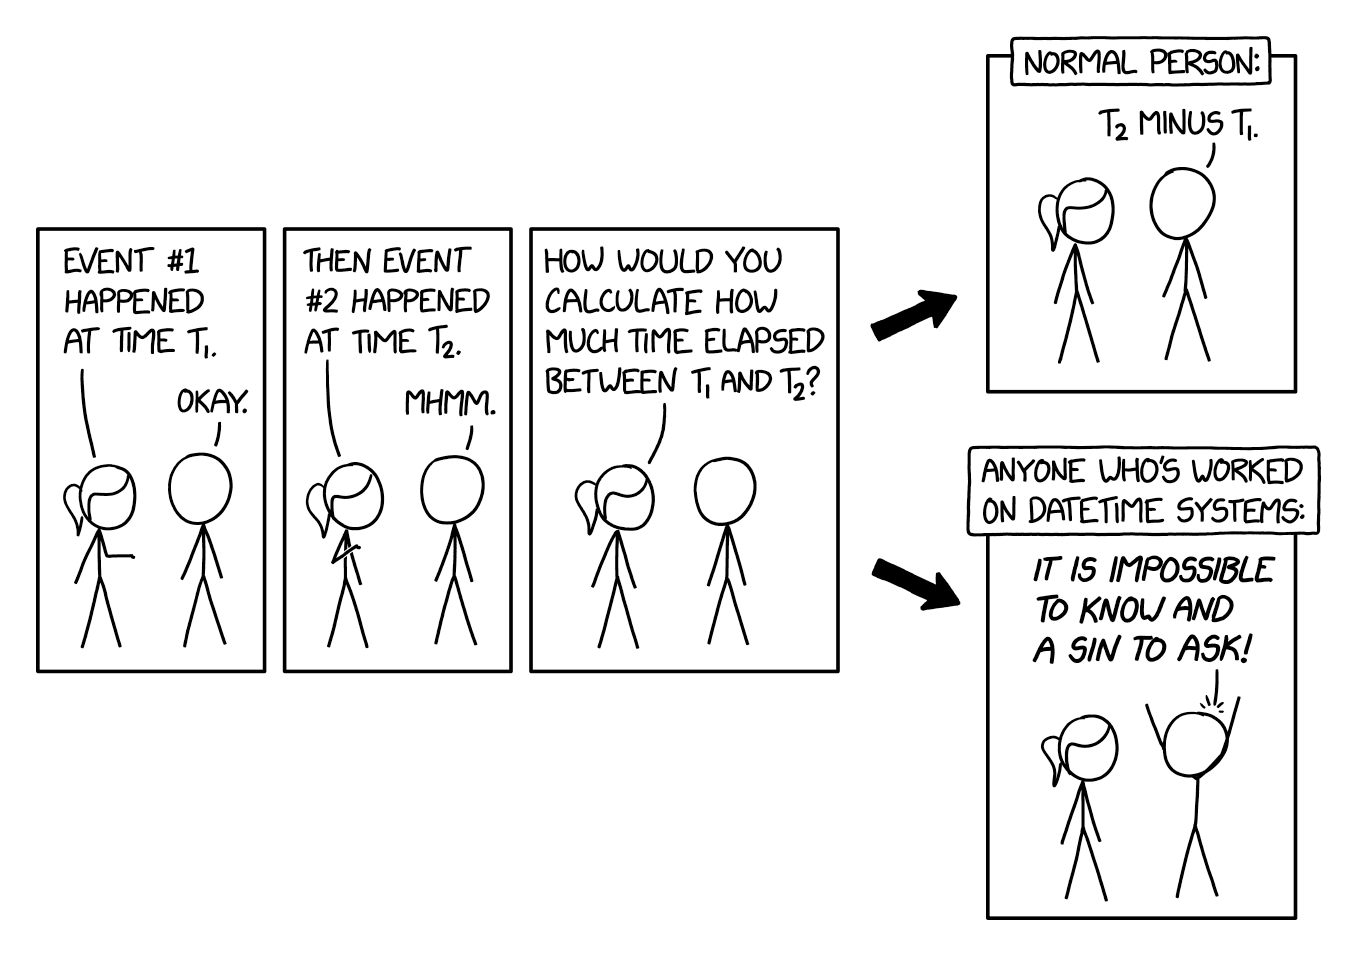
\includegraphics[align=t,width=0.75\linewidth]{images/datetime_2x.png}
% \\%
% \url{https://xkcd.com/2867}
% \end{figure}
UTC and TAI have the same time lapse, but UTC differ by irregular readjustments of its \enquote{zero}, the \furl{https://webtai.bipm.org/ftp/pub/tai/Circular-T/cirthtm/cirt.442.html}{leap seconds}.

The clock on your phone, and on devices synchronized via internet, shows UTC, not your proper time. An observer on Earth at \qty{0}{m} over sea level, and not moving, measures a proper-time lapse equal to UTC or TAI (besides small variations coming from the irregularity and internal motions of the Earth). But observers at other altitudes and observers moving with respect to Earth's surface can measure that their proper-times lapses are slightly different from UTC and TAI.

\medskip

In applications related to interplanetary spacecraft navigation and cosmological observations, the Barycentric Coordinate Time TCB is used. Its time lapse is slightly faster than the one of UTC: for each second that passes in UTC, \qty{1.0000000148}{s} pass in TCB on average. Two coordinate times to be used around an on the Moon, \furl{https://doi.org/10.1103/Physics.17.140}{Lunar Coordinate Time TCL} and Lunar Time LT, are on the making in the year 2025. Lunar Time will lapse faster by \qty{5.6e-5}{s} per day compared to our UTC. The establishment of all these kinds of coordinate times shows how important the difference between coordinate and proper time is for our current technology.

\medskip

When we use coordinate time, some important physics formulae turn out to be the same no matter whether we use General Relativity or an approximate theory such as Newtonian Mechanics. Thanks to this fact, for the most part of these notes we will not need to deal with proper-time details. But it is important for you to keep in mind how time really works, and the small time discrepancies that exist and occur all the time along your \emph{worldline}.



\section{Space, length, distance}
\label{sec:difficulties_distance}

Together with the notion of time, also the notions of space, length, distance lose some of their traditional intuition. Traditionally when we speak of the distance or the length of a moving object at a given time, we mean the distance \enquote*{at the same instant of time}. But we have seen that it does not make sense to ask \enquote{what is the time for the object, right now?}. And when we speak of lengths or distances, we mean measurements \enquote*{on a straight line}. But spacetime is curved.

To see the complications in defining \enquote*{distance} and \enquote*{length}, imagine two objects or people that are moving with respect to each other, getting closer and farther away. Call them A and B; let's say that A represents you. You have a clock, and B is equipped with another clock identical to yours. These clocks were synchronized (to time 06:00) in the past when you and B were in contact with each another.

%
\marginpar{\vspace{0\baselineskip}\footnotesize%
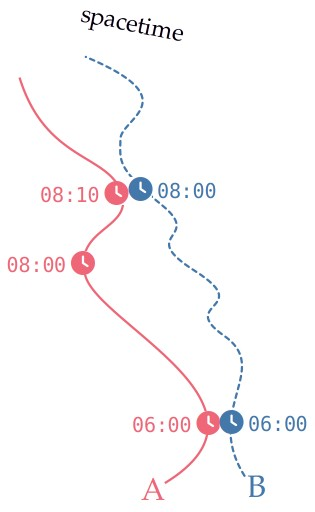
\includegraphics[width=\linewidth]{images/A_B_spacetime.jpg}%
% \\[\jot]%
% \footnotesize\color{mpcolor}%
}%
We can represent the motions of A and B as \emph{worldlines} in spacetime, as in the side figure (similarly to what we did in \fig~\ref{fig:ABC_spacetime}). The figure shows the points in spacetime where your clock displays the times 06:00, 08:00, and 08:10, and where B's clock displays 06:00 and 08:00. Note in particular that you and B touch each other and are synchronized at 06:00; then you touch each other again later, when your clock displays 08:10 and B's clock displays 08:00.

\medskip

Suppose that when your clock displays time 08:00 you ask \enquote{how distant is B from me \emph{right now}?}. How can we measure or define such distance?

One possibility is to say that we measure the length of a straight line joining you at \emph{your} time 08:00, with B at \emph{its} time 08:00. Could we define this as the distance between you and B at 08:00? Well, there's something bizarre: when B's clock shows 08:00, B is in contact with you! So we would essentially be measuring the distance between you and yourself at two different times of your clock. This doesn't seem to be very sensible. Also, should this distance be zero, then? But when your clock displayed 08:00, B was \emph{not} in contact with you, so it wouldn't make sense to say that its distance from you was zero.

So let's discard the measurement procedure above, which seems to inconsistent results. Another possibility is to measure the length of a straight line joining you at your time 08:00, with B at some other time on its clock. But which time should we choose? Any choice seems arbitrary.

And there's one more problem. Let's say that we decide to measure the distance between you when your clock shows 08:00, and B when its clock shows 07:50 or some other arbitrary time when it is not in contact with you. We should measure this distance on a straight line. But what's a \enquote*{straight line}? Spacetime is curved. A straight line in the figure above is not necessarily a straight line in spacetime. The notion closest to a \enquote*{straight line} in a curved space is that of a \furl{https://mathworld.wolfram.com/Geodesic.html}{\emph{geodesic}}. It turns out that there may be several geodesics connecting you (at 08:00) and B (at 07:50).

Similar problems appear if we ask questions about \emph{lengths}. Suppose there is a rubber band stretched between you (remember you're A) and B. When your clock shows 08:00 you ask \enquote{how long, \emph{right now}, is the rubber band joining me and B?} We encounter the same difficulties as above in trying to answer this question.

\medskip

% %
% \marginpar{\vspace{0\baselineskip}\footnotesize\centering%
% %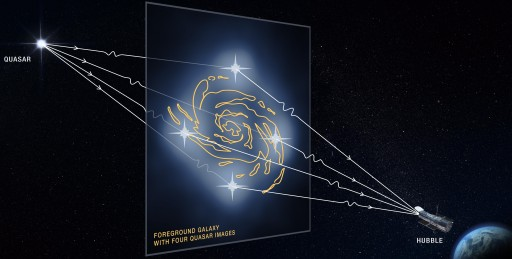
\includegraphics[width=\linewidth]{images/gravitational_lens3.jpg}%
% 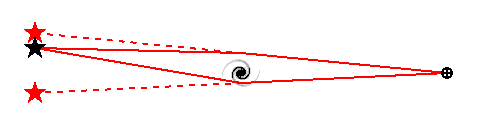
\includegraphics[width=\linewidth]{images/gravitational_lens1.png}%
% \\[2ex]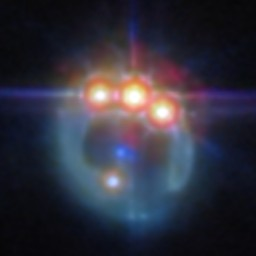
\includegraphics[width=\linewidth]{images/quasar_lens2.jpg}%
% \\[\jot]\flushleftright\color{mpcolor}Top: from
% %\furl{https://www.jpl.nasa.gov/images/pia23641-gravitational-lensing-graphic}{NASA JPL}.
% \emph{\furl{https://www.astro.ucla.edu/~wright/distance.htm}{The ABC's of Distances}}.
% Bottom: from \furl{https://esawebb.org/images/potm2406a}{ESA/Webb}.%
% }%
%
\marginpar{\vspace{0\baselineskip}\footnotesize\centering%
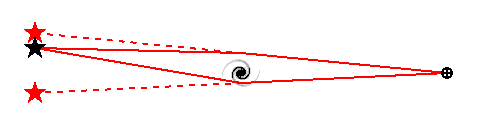
\includegraphics[width=\linewidth]{images/gravitational_lens1.png}%
\\[\jot]\footnotesize\flushleftright\color{mpcolor}From
\emph{\furl{https://www.astro.ucla.edu/~wright/distance.htm}{The ABC's of Distances}}.%
}%
\marginpar{\vspace{0\baselineskip}\footnotesize\centering%
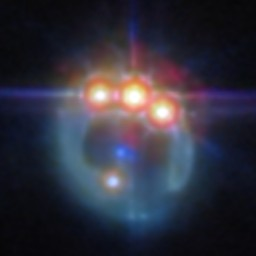
\includegraphics[width=\linewidth]{images/quasar_lens2.jpg}%
\\[\jot]\footnotesize\flushleftright\color{mpcolor}From \furl{https://esawebb.org/images/potm2406a}{ESA/Webb}.%
}%
A spectacular case of the effect of spacetime curvature is the phenomenon of \furl{https://science.nasa.gov/mission/hubble/science/science-behind-the-discoveries/hubble-gravitational-lenses}{gravitational lensing}. Owing to the curvature of spacetime, light and other electromagnetic radiation emanating from the object reach us along different paths in spacetime. All these paths are \enquote{straight lines} (geodesics). Coming from different directions, to us these look like distorted, duplicated images of the object, as schematized in the top side figure. The curvature is generated by some large distribution of \energym, such as a galaxy, between us and the object. A beautiful example of this phenomenon is given by the \furl{https://www.nasa.gov/image-article/distant-quasar-rx-j1131}{quasar RX~J1131-1231}, bottom side image. Spacetime curvature separates the light arriving to us from this quasar into four \textcolor{yellow}{yellow} \amp\ \textcolor{red}{red} spots, three at the top and one at the bottom in the image. The curvature is generated by a galaxy visible as the \textcolor{blue}{blue spot} at the centre.% but get also deformed into the almost-closed \textcolor{blue}{blue arc}.

\medskip

A consequence of these peculiar situations and of the curvature of spacetime is that many notions of distances and length can be defined and measured, which are generally \emph{not} equivalent to one another. Cosmology, for example, uses a \furl{https://doi.org/10.48550/arXiv.astro-ph/9905116}{plethora of different distances}. One must therefore be careful about which definition of distance is being used. In the next sections we shall focus on two of them: \emph{radar distance} and \emph{coordinate distance}.

% And there may be different paths having shortest distance; therefore saying \enquote{the path of shortest distance} may be ambiguous.


\section{Radar distance}
\label{sec:radar_distance}

The definition of distance that's regarded as the most \enquote{physical} is \emph{radar distance}, defined as follows.

Consider again a situation in which an object B is moving with respect to you. Yours and B's motions in spacetime, around the time when your clock displays time $t$, are illustrated in the next side figure.
Your \emph{worldline} in spacetime is the \textcolor{blue}{blue} one on the left; the worldline of object~B is the \textcolor{green}{green} one on the right. At your proper time $\yti$ you send a light pulse towards object~B. The pulse travels in empty space, and upon hitting object~B it immediately bounces back to you. It reaches you at your proper time $\ytf$. The worldline of the light pulse is shown in \textcolor{yellow}{dashed yellow} in the figure.
%
\marginpar{\vspace{-8\baselineskip}\footnotesize\centering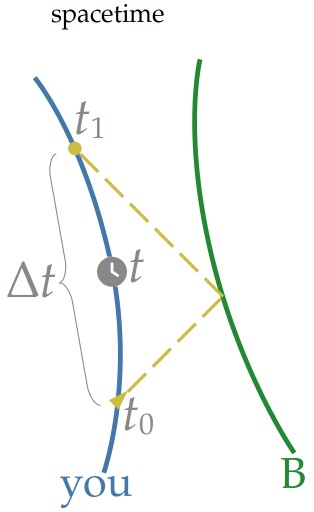
\includegraphics[width=0.9\linewidth]{images/radar_distance.jpg}%
  % \\[\jot]\flushleftright\color{mpcolor}%
}%

A proper time $\Dt = \ytf - \yti$ has elapsed for you between emission and reception of the light pulse, and the time exactly in between emission and reception is $t = (\ytf + \yti)/2$. The \textbf{radar distance} $d$ of object~B from you at time $t$ is defined as
\begin{equation}
  \label{eq:physical_distance}
  d \defd \tfrac12 c\, \Dt
\end{equation}
where $\yc$ is the speed of light in vacuum, a universal physical constant:
% %
% \marginpar{\vspace{-\baselineskip}\footnotesize%
% \color{mpcolor}The SI symbol for the speed of light in vacuum is \enquote{$c_{0}$} \parencites[item~6-35.2]{iso2008}. For simplicity we shall omit the subscript \enquote{${}_{0}$} in these notes.%
% }%
\begin{equation}
  \label{eq:c}
  \yc = \qty{299792458}{m/s}\quad\text{(exactly).}
\end{equation}

The SI unit of length, the \furl{https://www.nist.gov/si-redefinition/meter}{metre}, is based on the measuring procedure above. Common laser distance meters also work by the same procedure, and therefore yield radar distance. As the name indicates, this is also the distance measured by radars.
%
\marginpar{\vspace{-3\baselineskip}\footnotesize\centering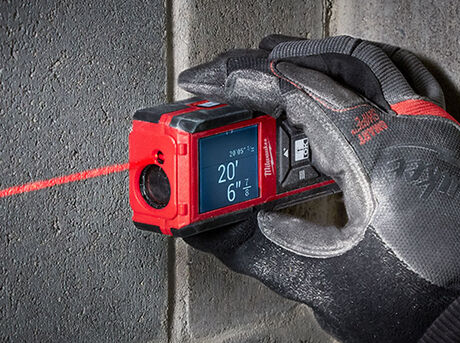
\includegraphics[width=0.75\linewidth]{images/laser_meter.jpg}%
\\[\jot]\flushleftright\color{mpcolor}A laser distance meter (the light beam is not visible in reality).%
}%

In using radar distance, however, we must be wary of the following peculiarities:
\begin{itemize}[wide]
\item Radar distance makes sense only if the time lapse $\Dt$ is small enough compared to variations in the relative motion of the observer and the object, so that this motion is approximately uniform. For this reason this distance cannot be used if the object is too far away: the farther away it is, the longer it takes for a light beam to travel to and fro. Radar distance can be used between the Earth and other Solar System planets; but it cannot be used for galaxies or other distant cosmological objects.

\item \textbf{Radar distance is not symmetric}: the radar distance of B from A at A's time $t$ is generally different from the radar distance of A from B at B's time $t$.

\item \textbf{The value of radar distance depends on the relative motion} between A and B. Imagine that a friend of yours is located very close to you at time $t$, but is moving with respect to you. Upon measuring object~B's radar distance, your friend will generally find a value different from yours. The discrepancy between you and your friend's measured values will be the larger, the higher is the relative velocity between you two. Several observers in motion with respect to one another will generally disagree on the dimensions of an approximately rigid objects in their vicinity.
\end{itemize}

%
\marginpar{\vspace{-3\baselineskip}\footnotesize\centering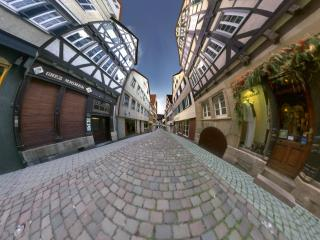
\includegraphics[width=\linewidth]{images/tuebingen.jpg}%
  \\[\jot]\flushleftright\color{mpcolor}How a street in T{\"u}bingen would look like (except for colour and some other features) if we travelled through it at around \qty{240000000}{m/s} (from \textit{\furl{https://www.spacetimetravel.org/}{Relativity visualized}})%
}%
The dependence on relative motion also affects, at high speeds, how we \emph{see} objects, which appears more and more deformed. You can find beautiful visualizations, both static and animated, at \textit{\furl{https://www.spacetimetravel.org/}{Relativity visualized}}.


\medskip

Luckily, for relative speeds that are not too high compared to the speed of light, the radar distances measured by different observers differ by amounts that are negligible in everyday circumstances. As an example, consider a car moving on a road at \qty{100}{km/h}, that is around \qty{28}{m/s}. The car's driver measures the length of the car to be \qty{4}{m} by radar distance. A pedestrian that sees the car passing by instead measures its length to be \qty{3.99999999999998}{m} by radar distance. This is obviously a negligible difference.

\medskip

Length and distance have SI dimension \textsc{length}, and we shall usually measure them using the unit \emph{metre}, symbol \enquote*{$\unit{m}$}.

\begin{exercise}[label={ex:distance}]
  % **** Add figure
  Imagine that you and a friend of yours are measuring your distance from a wall, using a laser distance meter each. You and the wall are static with respect to Earth's surface. Your friend is moving with a speed $v$ towards the wall, and is right beside you at the exact moment of the measurement.

  \smallskip

  In this specific situation, if $d_{\textrm{you}}$ is the distance measured by you, and $d_{\textrm{friend}}$ the distance measured by your friend, the two are related by the formula
  \begin{equation*}
    d_{\textrm{friend}} = d_{\textrm{you}} \cdot \sqrt{1 - v^{2}/\yc^{2}} \ ,
  \end{equation*}
  where $\yc$ is the speed of light, given in \eqn~\eqref{eq:c}. Note that this formula is also valid if your friend is moving away from the wall, rather than towards it.

\begin{enumerate}[exerc]
\item\label{item:distance_friend} Suppose you find that the distance of the wall from you is \qty{200}{m}. Your friend's speed is \qty{300}{m/s}. How much is the distance from the wall to your friend, who's right beside you, as measured by your friend? (You'll need a high-precision calculator and 18 significant digits.)

\item\label{item:velocity_friend} Now instead suppose you find that the distance of the wall from you is \qty{500}{m}. Your friend measured (when right beside you) a distance of \qty{499}{m}. How fast was your friend moving?
\end{enumerate}
\end{exercise}

\section{Coordinate systems}
\label{sec:coords}

\marginpar{\vspace{\baselineskip}\footnotesize\color{mpcolor}\enquote{\emph{%
% The views of space and time which I wish to lay before you have sprung from the soil of experimental physics, and therein lies their strength. They are radical.
Henceforth, space by itself, and time by itself, are doomed to fade away into mere shadows, and only a kind of union of the two will preserve an independent reality.}}\sourceatright{\cites{minkowski1908b}}
}
%
From our discussion about time and space we conclude that physical events happen in spacetime, and there is no unique way to attribute a universal time or a universal position in space to a physical event.
% There is one absolute: whoever locally measures the physical speed of light in empty space, will find the value $\yc$. This value, exact by definition, serves as a way to define a local notion of space and distance.

In the previous sections we used the word \enquote*{event}, informally taking its meaning for granted. Let's be more precise now. We call \textbf{event} or \textbf{spacetime point} a very small region of space that lasts for a very short lapse of time, so  that it can be considered as a point in a four-dimensional space. When we say \enquote*{small region} or \enquote*{short time lapse}, it doesn't matter which definition of distance or time lapse we're using.

The word \enquote*{event} is used because typically we identify such a spacetime point by means of a physical phenomenon of limited spatial extension and duration. How \enquote{limited} should these extension and duration be? It depends on the kind of physical phenomenon we're interested in. The sudden burst of a soap bubble can be considered as an event in comparison to geological distances and times; but it cannot be considered as an event if we're studying subatomic particles.

% An object like a tennis ball can in some circumstances be considered as a point \emph{in space}; but it cannot be considered as an event because it persists for quite a long time, not just for a short instant. From the point of view of four-dimensional spacetime, such an object can be characterized as a line: a \textbf{worldline}.

\medskip

The peculiarities of spacetime can make it difficult to communicate the positions of objects and events by relying on distances. In giving indications about the location of a shop we can say \enquote{it's 200 metres down the road} without ambiguity. But in situations where much higher precision is needed and extreme motions or gravitational fields are involved, we would need to know the velocity of the person we're talking to, because the distances measured by us and by that person could be very different. % Moreover, the communication of locations usually involves reference to places that are known to all parties involved in the communication.


In the case of time, we bypassed the problem that time lapse depends on the observer's motion by introducing a \autoref{sec:coord_time}{coordinate time}. This way each event gets an arbitrary but agreed-upon time label. We can bypass the analogous problem that length and distance depend on the observer's motion, by introducing a set of arbitrary \emph{spatial coordinates} for each coordinate time.

All these coordinates together form a \emph{coordinate system}, also called \emph{reference system}:
\begin{definition}{Coordinate system or reference system}\label{def:coordinates}
  A \textbf{coordinate system}, also called \textbf{reference system}, is the assignment, by agreement, of four numerical labels to every point in spacetime: one \emph{coordinate time} and three \emph{spatial coordinates}. We use symbols such as $(t,x,y,z)$, or $(t, r, \theta,\phi)$, or others, for these coordinates. These four coordinates are obviously the same for all observers, because they are decided by agreement.

  \smallskip
  
   A coordinate system is usually defined on a limited region of spacetime.

  \smallskip

  The location where all spatial coordinates have value zero is called the \textbf{origin} of the spatial coordinates.
\end{definition}
% % 
% \marginpar{\vspace{-\baselineskip}\footnotesize\centering%
% 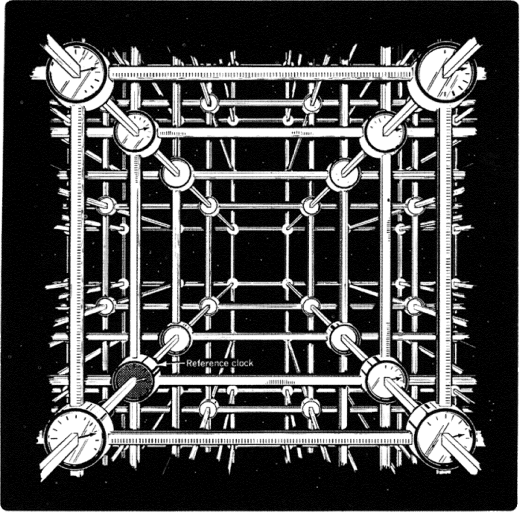
\includegraphics[width=\linewidth]{images/lattice_meters_clocks2.png}
% \\[\jot]\footnotesize\flushleftright\color{mpcolor}%
% A lattice of clocks and meters, defining a spacetime coordinate system (from \cites{tayloretal2000})%
% }%

  Often the coordinates have physical meaning -- like the proper time elapsed for a specific clock, or the distance from some event as measured by a specific observer -- but they don't need to. Typically we use three spatial coordinates. In special situations, such as locating points on the Earth's surface neglecting altitude, only two or even one spatial coordinate can be enough.


%
\marginpar{\vspace{0\baselineskip}\footnotesize\centering%
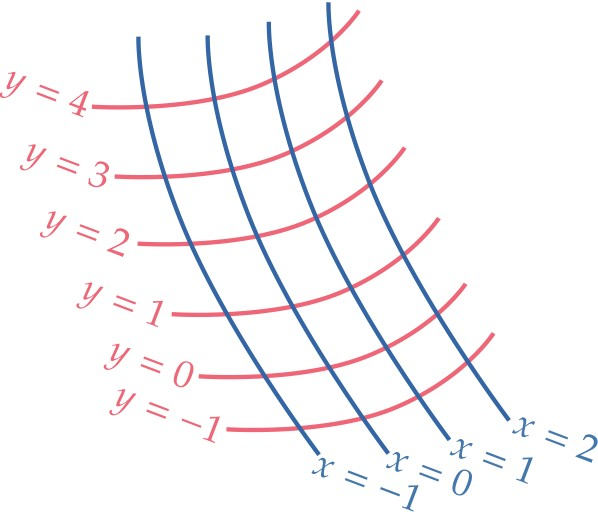
\includegraphics[width=\linewidth]{images/coords_curv.jpg}%
% \\[\jot]\footnotesize\flushleftright\color{mpcolor}%
% Grid representing a two-dimensional coordinate system.%
}%
A coordinate system can be visualized as a grid made by a set of lines or planes, one set for each coordinate, which allow us to read the coordinates of any point. The side figure shows an example with spatial coordinates $(x,y)$ in two dimensions, for a specific coordinate time. It is of course assumed that the grid can be refined as much as needed. We are all familiar with the coordinate system $(\lambda, \phi)$ of \emph{latitude} and \emph{longitude} to identify locations on Earth's surface, and used internally by the location systems of mobile phones.

Since a coordinate system is arbitrary, we often choose one adapted to the physical phenomenon under study. It's very common to choose a coordinate system $(t,x,y,z)$ that has time coordinate $t=\qty{0}{s}$ at the beginning of our observation of the phenomenon, and spatial coordinates $(x,y,z)=(0,0,0)\,\unit{m}$ at a location close to where the phenomenon happens.

\medskip

The spatial coordinates may be chosen so as to have particular physical properties, which in turn may lead to simpler expressions for some physical laws \autoref{sec:constitutive}{as we shall see later}. For instance, the coordinate lines of might be straight lines (geodesics), in which case we speak of \emph{rectilinear coordinates}. If they are not, then we call them \emph{curvilinear coordinates}; the coordinates in the previous side figure are curvilinear.

If the spatial coordinate lines are \emph{orthogonal} to one another at every point, that is, they intersect at $\pi/2\,\unit{rad}$, then we call them \textbf{orthogonal coordinates}. This is a very useful property, which simplifies many physics formulae. In these notes we shall always use orthogonal coordinates. Note that a coordinate system can be curvilinear \emph{and} orthogonal.

\medskip

In astronomy, in space and satellite communication, and in \furl{https://oceanservice.noaa.gov/geodesy}{geodesy} (the science of accurately measuring and understanding the Earth's geometric shape, orientation in space, and gravity field), \furl{https://gssc.esa.int/navipedia/index.php?title=Reference_Systems_and_Frames}{several important coordinate systems} are used. For example:

\begin{itemize}
\item%
\marginpar{\vspace{0\baselineskip}\footnotesize\centering%
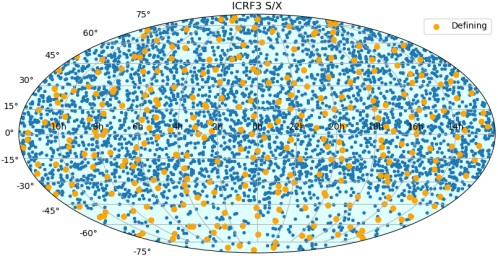
\includegraphics[width=\linewidth]{images/icrf3sx.jpg}%
\\[\jot]\flushleftright\color{mpcolor}%
Map of some distant astronomical objects used to define the International Celestial Reference Frame (from \furl{https://hpiers.obspm.fr/icrs-pc/newwww/icrf/index.php}{\emph{The ICRF}}).%
}%
 The \furl{https://aa.usno.navy.mil/faq/ICRS_doc}{\emph{International Celestial Reference System} (ICRS)} is a coordinate system with orthogonal spatial coordinates, which are almost rectilinear. Their origin is close to the centre of the Sun. Several distant cosmological objects, like \furl{https://esahubble.org/wordbank/quasar}{quasars}, have fixed spatial coordinates in this reference system. Its coordinate time is called Barycentric Coordinate Time (TCB).


\item The \emph{Geocentric Celestial Reference System} (CGRS) is a coordinate system with orthogonal spatial coordinates, which are almost rectilinear. Their origin is close to the centre of the Earth. Distant cosmological objects have almost constant spatial coordinates in this reference system; this means that the Earth rotates with respect to it. Its coordinate time is called Geocentric Coordinate Time (TGB), which is very similar to the TAI.

\item The \furl{https://itrf.ign.fr/en/background}{\emph{International Terrestrial Reference System} (ITRS)} is a coordinate system similar to the CGRS, but with the important difference that the Earth is approximately static in this reference system; this means that distant cosmological objects rotate with respect to it. It has the same coordinate time as the ICRS.

\item The \furl{https://earth-info.nga.mil/?dir=wgs84\&action=wgs84}{\emph{World Geodetic System 1984} (WGS~84)} is very similar to the ITRS, besides a discrepancy of some centimetres. It is used by the system of GPS satellites.
\end{itemize}

But how do we determine the position and time of an event in these coordinate systems? The procedure can be extremely complicated in fact. The starting point is the assignment of some predefined coordinates to objects that seem to have fixed spatial coordinates in the coordinate system; for instance distant cosmological objects like \furl{https://esahubble.org/wordbank/quasar}{quasars} in the case of the ICRS and CGRS, or \furl{https://itrf.ign.fr/en/solutions/ITRF2020-u2023\#frame-definition}{particular reference stations} on Earth's surface in the case of the ITRS and WGS~84. The coordinate of other events are then calculated from measurements of proper times, radar distances, and angles from the reference objects, using formulae from general relativity. As we mentioned in \sect\,\ref{sec:time}, even your mobile phone participates in these complex calculations.
%
\marginpar{\vspace{-10\baselineskip}\footnotesize\centering%
  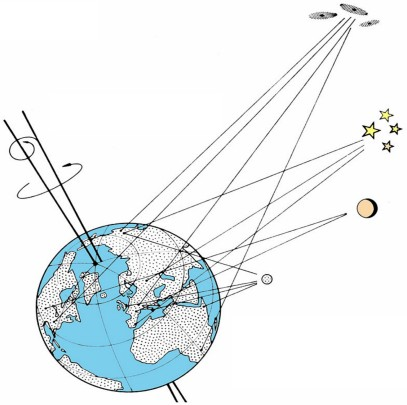
\includegraphics[width=\linewidth]{images/gcrf.jpg}
  \\[\jot]\footnotesize\flushleftright\color{mpcolor}%
  The assignment of coordinates on and around Earth depends on nominal values assigned to distant astronomical objects (from \cites{capitaine2010})%
}%

\begin{exercise}[label={ex:latlong}]
  % **** Add figure
  On Earth's surface we often use the system of two coordinates called \emph{latitude} $\lambda$ and \emph{longitude} $\phi$, measured in degrees. Coordinate lines of constant latitude are called \emph{parallels}; those of constant longitude are called \emph{meridians}.
  % Earth's surface is curved, and the \enquote{straight lines} in this space are maximal circles. All the meridians are maximal circles; therefore longitude is \emph{not} a curvilinear coordinate.

  \begin{enumerate}[exerc]
  % \item\label{item:latitude_curvilinear} Is latitude a curvilinear coordinate? Explain why or why not.
  \item Find what's at these three coordinate pairs:
    \begin{equation*}
      \begin{aligned}
        (\lambda, \phi) &= (\qty{60.369002}{\degree}, \qty{5.350336}{\degree})
        \\
        (\lambda, \phi) &= (\qty{35.658587}{\degree}, \qty{139.745424}{\degree})
        \\
        (\lambda, \phi) &= (\qty{-13.163069}{\degree}, \qty{-72.545265}{\degree})
      \end{aligned}
    \end{equation*}

  \item Are latitude and longitude \emph{orthogonal} coordinates? Explain why or why not.
  \end{enumerate}
\end{exercise}
% In Bergen, a distance of 10\,m corresponds to a difference of 0.000\,1\,degree in latitude or longitude


\section{Spatial coordinate distance and length}
\label{sec:coord_distance}

If we have chosen a coordinate system, we can define a notion of distance called
%\emph{coordinate length}  and % eg in \autocites{misneretal1970_r2017}
\emph{coordinate distance} between two points % eg in \autocites{peebles1993,weinberg1972}
at any coordinate time $t$. The idea is simple: we measure the length of the shortest path in spacetime joining the two points, and all intermediate points on the path must have the same coordinate time $t$. Of course it can happen that there is more than one path having shortest length.

Coordinate distance is different from radar distance. It has two advantages: it doesn't depend on relative motion, and can be defined also between objects that are very far apart. In regions of spacetime with low curvature and slow relative motions, however, radar distance and coordinate distance based on standard coordinate times are approximately the same, and approximately independent of any motions.

Note also that the speed of light defined with respect to coordinate distance need not have the value $\yc$, or even be constant! You might have heard or read about  distant cosmological objects, like quasars, that are said to be receding from us at speeds faster than light's. How is that possible? The reason is that the \enquote*{speeds} they're talking about are defined with respect to coordinate distance, not radar distance.

\medskip

\begin{definition}{Cartesian coordinates}\label{def:cartesian_coords}
We call \textbf{Cartesian coordinates} a set of spatial coordinates $(x,y,z)$ with a very special property: the coordinate distance between two locations A and B having spatial coordinates $(x_{\textrm{A}}, y_{\textrm{A}}, z_{\textrm{A}})$ and $(x_{\textrm{B}}, y_{\textrm{B}}, z_{\textrm{B}})$ is simply given by
\begin{equation}
  \label{eq:distance_cartesian}
  d_{\textrm{A}\textrm{B}} = \sqrt{
    (x_{\textrm{B}} - x_{\textrm{A}})^{2} +
    (y_{\textrm{B}} - y_{\textrm{A}})^{2} +
    (z_{\textrm{B}} - z_{\textrm{A}})^{2}
  } \ .
\end{equation}
\end{definition}

Perfect Cartesian coordinates do not exist, because spacetime is curved. But it is possible to choose coordinates that are approximately Cartesian in limited regions of spacetime. The coordinate systems ICRS, GCRS, ITRS discussed in \sect\,\ref{sec:coords} are \emph{not} Cartesian: they include the effects of curvature generated by the Earth and other bodies in the Solar System.

In most of these notes we will not have to worry about the discrepancies between radar distance and coordinate distance, and about the motion of the observer or instrument that is measuring a distance. So we shall use the term \enquote*{distance} without specifications. And we shall often use Cartesian coordinates.

\begin{exercise}
  In the Geocentric Celestial Reference System, defined by the International Astronomical Union, the distance between two very close locations A and B having spatial coordinates $(x_{\textrm{A}}, y_{\textrm{A}}, z_{\textrm{A}})$ and $(x_{\textrm{B}}, y_{\textrm{B}}, z_{\textrm{B}})$ close to Earth's surface is approximately given by
\begin{equation}
  \label{eq:distance_GCRS}
  d_{\textrm{GCRS},\textrm{A}\textrm{B}} = \bigl(1 + g R/\yc^{2}\bigr)
  \sqrt{
    (x_{\textrm{B}} - x_{\textrm{A}})^{2} +
    (y_{\textrm{B}} - y_{\textrm{A}})^{2} +
    (z_{\textrm{B}} - z_{\textrm{A}})^{2}
  }
\end{equation}
where $g \approx \qty{9.8}{m/s^{2}}$ is the gravitational accelaration, $R \approx \qty{6371e3}{m}$ is Earth's radius, and $\yc$ is the speed of light. This is also the radar distance of B from A, if A is not moving with respect to the coordinate system.
\begin{enumerate}[exerc]
\item Verify that the formula above is dimensionally correct: both left and right side should have dimension \textsc{length}.
\item Assume that your coordinates are $(x_{\textrm{A}}, y_{\textrm{A}}, z_{\textrm{A}})$, and consider an object B at a $x$-coordinate difference of \qty{100}{m} from you, that is, with coordinates
  \begin{equation*}
    x_{\textrm{B}} = x_{\textrm{A}} + \qty{100}{m}
    \ ,\qquad
    y_{\textrm{B}} = y_{\textrm{A}}
    \ ,\qquad
    z_{\textrm{B}} = z_{\textrm{A}} \ .
  \end{equation*}
  How much is the difference between the distances $d_{\textrm{A}\textrm{B}}$ and $d_{\textrm{GCRS},\textrm{A}\textrm{B}}$, calculated between you and the object?

  \emph{(The inaccuracy in the specification of $g$ and $R$ is actually much larger than the difference you just found.)}
  %\qty{7e-8}{m}
\end{enumerate}
\end{exercise}

\section{Coordinate position}
\label{sec:position_vector}

Let us agree on some notation and terminology that will be used in these notes.

\medskip

We shall often denote the four coordinates of a coordinate system by the letters
\begin{equation*}
  (t, x, y, z) \ .
\end{equation*}
Unless stated otherwise, the coordinate time $t$ will be taken to be \autoref{sec:coord_time}{UTC}, and the spatial coordinates $(x,y,r)$ will be taken to be \autoref{def:cartesian_coords}{Cartesian}. As mentioned in the previous section, the definition of the spatial coordinates is usually different from problem to problem; so it is always important to specify how the coordinate system you're using is defined.

\begin{definition}{Position or location vector}\label{def:position_vect}
The triplet of spatial coordinates is called the \textbf{position} or \textbf{location} vector and is often denoted by $\yr$:
\begin{equation*}
  \yr \defd (x,y,z)
  \qquad\text{or}\qquad
  \yr \defd [x,y,z]
  \qquad\text{or}\qquad
  \yr \defd
  \begin{bmatrix}
    x\\y\\z
  \end{bmatrix}
\end{equation*}
\end{definition}
use round brackets \enquote*{$()$} or square brackets \enquote*{$[]$}, and horizontal or vertical notation as you prefer.

Whenever we speak of a \enquote{region of space} or of a \enquote{surface in space}, we mean a 3D or 2D region at some specific coordinate time $t$.

Some physical phenomena happen approximately along a line, in one dimension; think for instance of a small falling object. Other phenomena happen approximately on a surface, in two dimensions; think for instance of a swinging pendulum. In these cases we can omit two or one of the spatial coordinates, and simply assume that the omitted ones have some constant, unimportant values. In such cases we can simply write, for instance, $(t,x)$ or $(t,x,y)$ as our coordinates.

\section{Coordinate velocity and acceleration}
\label{sec:velocity}

In some situations the spatial coordinates $\yr = (x,y,z)$ may be functions of the time coordinate $t$. A typical example is when we describe how the spatial position of a small volume or body changes with coordinate time. We can write this functional dependence in different ways, for instance
\begin{equation*}
  \yr(t)\quad\text{or}\quad
  \bigl[x(t)\,,\ y(t)\,,\ z(t)\bigr] \ .
\end{equation*}
So $\yr$ is a vector function of time, which simply means that we have a collection of three functions of time.


If we take the derivative of each coordinate with respect to the time $t$, we obtain the \emph{coordinate velocity}:

\begin{definition}{Coordinate velocity}\label{def:coord_velocity}
  The \textbf{coordinate velocity} is a vector defined as the derivative of the position vector $\yr(t)$ with respect to coordinate time $t$:
  \begin{equation*}
    \yv(t) %= \bigl[v_{x}(t)\ ,\ v_{y}(t) \ ,\ v_{z}(t) \bigr]
    \defd \frac{\di}{\dt}\yr(t)
    \quad\text{or}\quad
    \begin{bmatrix}
      v_{x}(t)\vphantom{\dfrac{\di}{\dt}}\\[3\jot]
      v_{y}(t)\vphantom{\dfrac{\di}{\dt}}\\[3\jot]
      v_{z}(t)\vphantom{\dfrac{\di}{\dt}}
    \end{bmatrix}
    \defd
    \begin{bmatrix}
      \dfrac{\di}{\dt} x(t)\\[3\jot]
      \dfrac{\di}{\dt} y(t)\\[3\jot]
      \dfrac{\di}{\dt} z(t)
    \end{bmatrix} \ .
  \end{equation*}

  \smallskip

  The word \textbf{speed} means the \emph{magnitude} of the velocity:
  \begin{equation*}
    \abs{\yv} \equiv \sqrt{{v_{x}}^{2} + {v_{y}}^{2} + {v_{z}}^{2}} \ .
  \end{equation*}

  \smallskip

    The derivative of some quantity with respect to coordinate time is often denoted by a \textbf{dot} over the quantity. So we can also write
    \begin{equation*}
      \yv(t) = \dot{\yr}(t) = \bigl[\dot{x}(t)\,,\ \dot{y}(t)\,,\ \dot{z}(t)\bigr]
    \end{equation*}
  \end{definition}
The coordinate velocity is usually different from the \emph{physical velocity}, which an observer would measure using proper time and space, for instance using bouncing light rays. In many everyday situations the difference between coordinate and physical velocity is so small that it can be neglected, so we shall simply use the word \enquote*{velocity}. But in situations involving subatomic particles at high speed, for example, one must take into account that the two velocities are different.

\medskip

Taking the derivative of the velocity with respect to coordinate time, that is, the second derivative of position, we obtain the \emph{coordinate acceleration}:
\begin{definition}{Coordinate acceleration}\label{def:coord_acceleration}
  The \textbf{coordinate acceleration} is a vector defined as the derivative of the velocity vector $\yv(t)$ with respect to coordinate time $t$:
\begin{equation*}
  \bm{a}(t) \defd \frac{\di}{\dt}\yv(t) =
  \frac{\di^{2}}{\dt^{2}}\yr(t) =
  \biggl[\frac{\di^{2}}{\dt^{2}} x(t)\,,\
  \frac{\di^{2}}{\dt^{2}} y(t)\,,\
  \frac{\di^{2}}{\dt^{2}} z(t)\biggr] \ .
\end{equation*}
\end{definition}

\begin{extra}{Acceleration in relativity theory}
  In relativity theory, acceleration has a special physical significance because it includes the effect of gravity. We distinguish between \emph{physical acceleration} and \emph{coordinate acceleration}. The calculation of physical acceleration  requires more than a time derivative.

  \smallskip

  For instance, let's say that you are standing still on the ground, and let's use a coordinate system where $x$ points in front of you, $y$ to your left, and $z$ upward. Then your coordinate velocity is $\yv=(0,0,0)\,\unit{m/s}$, also according to relativity theory. But your spatial \emph{physical} acceleration is approximately $(0,0,9.8)\,\unit{m/s^{2}}$, not zero!

  \smallskip

  The definitions and values of physical acceleration according to relativity theory and to Newtonian mechanics are therefore quite different even in everyday situations. In these notes we'll mean coordinate acceleration, unless stated otherwise. This is also the meaning in Newtonian mechanics.
\end{extra}


\subsection{Integration of velocity and acceleration}
\label{sec:integration_velocity}

Since velocity is the time derivative of position, we can find the position from the velocity by the inverse operation of integration. So we have
\begin{equation*}
  \yr(t) %= \bigl[v_{x}(t)\ ,\ v_{y}(t) \ ,\ v_{z}(t) \bigr]
  =  \yr(\yti) + \int_{\yti}^{t}\yv(t)\,\dt
  \qquad\text{or}\qquad
  \begin{bmatrix}
    x(t)\vphantom{\int_{\yti}^{t}}\\[3\jot]
    y(t)\vphantom{\int_{\yti}^{t}}\\[3\jot]
    z(t)\vphantom{\int_{\yti}^{t}}
  \end{bmatrix}
  =
  \begin{bmatrix}
    x(\yti)\vphantom{\int_{\yti}^{t}}\\[3\jot]
    y(\yti)\vphantom{\int_{\yti}^{t}}\\[3\jot]
    z(\yti)\vphantom{\int_{\yti}^{t}}
  \end{bmatrix} +
  \begin{bmatrix}
    \int_{\yti}^{t}v_{x}(t)\,\dt\\[3\jot]
    \int_{\yti}^{t}v_{y}(t)\,\dt\\[3\jot]
    \int_{\yti}^{t}v_{z}(t)\,\dt
  \end{bmatrix} \ .
\end{equation*}
Note from the formulae above that if we know the expression of the velocity $\yv(t)$, we still cannot know the position $\yr(t)$ unless we \emph{also} know the value $\yr(\yti)$ of the position at some particular time $\yti$.

  \medskip

In a analogous way we can find the velocity $\yv(t)$ from the acceleration $\bm{a}(t)$ by integration, provided we also know the value $\yv(\yti)$ of the velocity at some particular time $\yti$:
\begin{equation*}
  \yv(t) %= \bigl[a_{x}(t)\ ,\ a_{y}(t) \ ,\ a_{z}(t) \bigr]
  =  \yv(\yti) + \int_{\yti}^{t}\bm{a}(t)\,\dt
  \qquad\text{or}\qquad
  \begin{bmatrix}
    v_{x}(t)\vphantom{\int_{\yti}^{t}}\\[3\jot]
    v_{y}(t)\vphantom{\int_{\yti}^{t}}\\[3\jot]
    v_{z}(t)\vphantom{\int_{\yti}^{t}}
  \end{bmatrix}
  =
  \begin{bmatrix}
    v_{x}(\yti)\vphantom{\int_{\yti}^{t}}\\[3\jot]
    v_{y}(\yti)\vphantom{\int_{\yti}^{t}}\\[3\jot]
    v_{z}(\yti)\vphantom{\int_{\yti}^{t}}
  \end{bmatrix} +
  \begin{bmatrix}
    \int_{\yti}^{t}a_{x}(t)\,\dt\\[3\jot]
    \int_{\yti}^{t}a_{y}(t)\,\dt\\[3\jot]
    \int_{\yti}^{t}a_{z}(t)\,\dt
  \end{bmatrix} \ .
\end{equation*}

\begin{exercise}
  \begin{enumerate}[exerc]
  \item Here are the three components of a time-dependent velocity vector The variable $t$ is the time, and therefore has dimension \textsc{time}. Introduce units \enquote*{\unit{s}} and \enquote*{\unit{m}}  in such a way that the expression is dimensionally correct:
    \begin{equation*}
      \bm{v}(t) = \bigl[4, \cos(3\,t), -\exp(8/t)\bigr]
    \end{equation*}
  \item The position vector of a satellite is given below. Calculate the satellite's velocity and acceleration vectors:
    \begin{equation*}
      \yr(t) =
      \begin{bmatrix}
        \num[exponent-mode=scientific]{20e6}\,
        \cos\bigl(\frac{t}{\qty{13751}{s}}\bigr)\\[2\jot]
        \num[exponent-mode=scientific]{22e6}\,
        \sin\bigl(\frac{t}{\qty{13751}{s}}\bigr)\\[2\jot]
        \num{0}
      \end{bmatrix}\,\unit{m}
    \end{equation*}
  \item What is the satellite's velocity at $t=\qty{6875}{s}$? What is the magnitude of the velocity (that is, the speed)?

  \item Suppose you know the expression of the \emph{speed} $v(t) \equiv \abs{\yv(t)}$ of an object, and also the object's position $\yr(\yti)$ at time $\yti$. From this information, can you find the position $\yr(t)$ at any other time $t$?
  \end{enumerate}
\end{exercise}



\section{Angles}
\label{sec:angles}

\mynotew{To be written.}




% \begin{subappendices}
%
% \addsec{\color{green}\faIcon{puzzle-piece}\enskip Exercises\enskip\faIcon{puzzle-piece}}
%
% % \setsecnumformat{E\upshape\oldstylenums{\csname the#1\endcsname\quad}}
% % \setsecnumformat{\sectionname\
% % \oldstylenums{\csname the#1\endcsname\quad}}
%
% \exsubsec{\ref{sec:coords}}
%
% \marginpar{\footnotesize\centering%
%   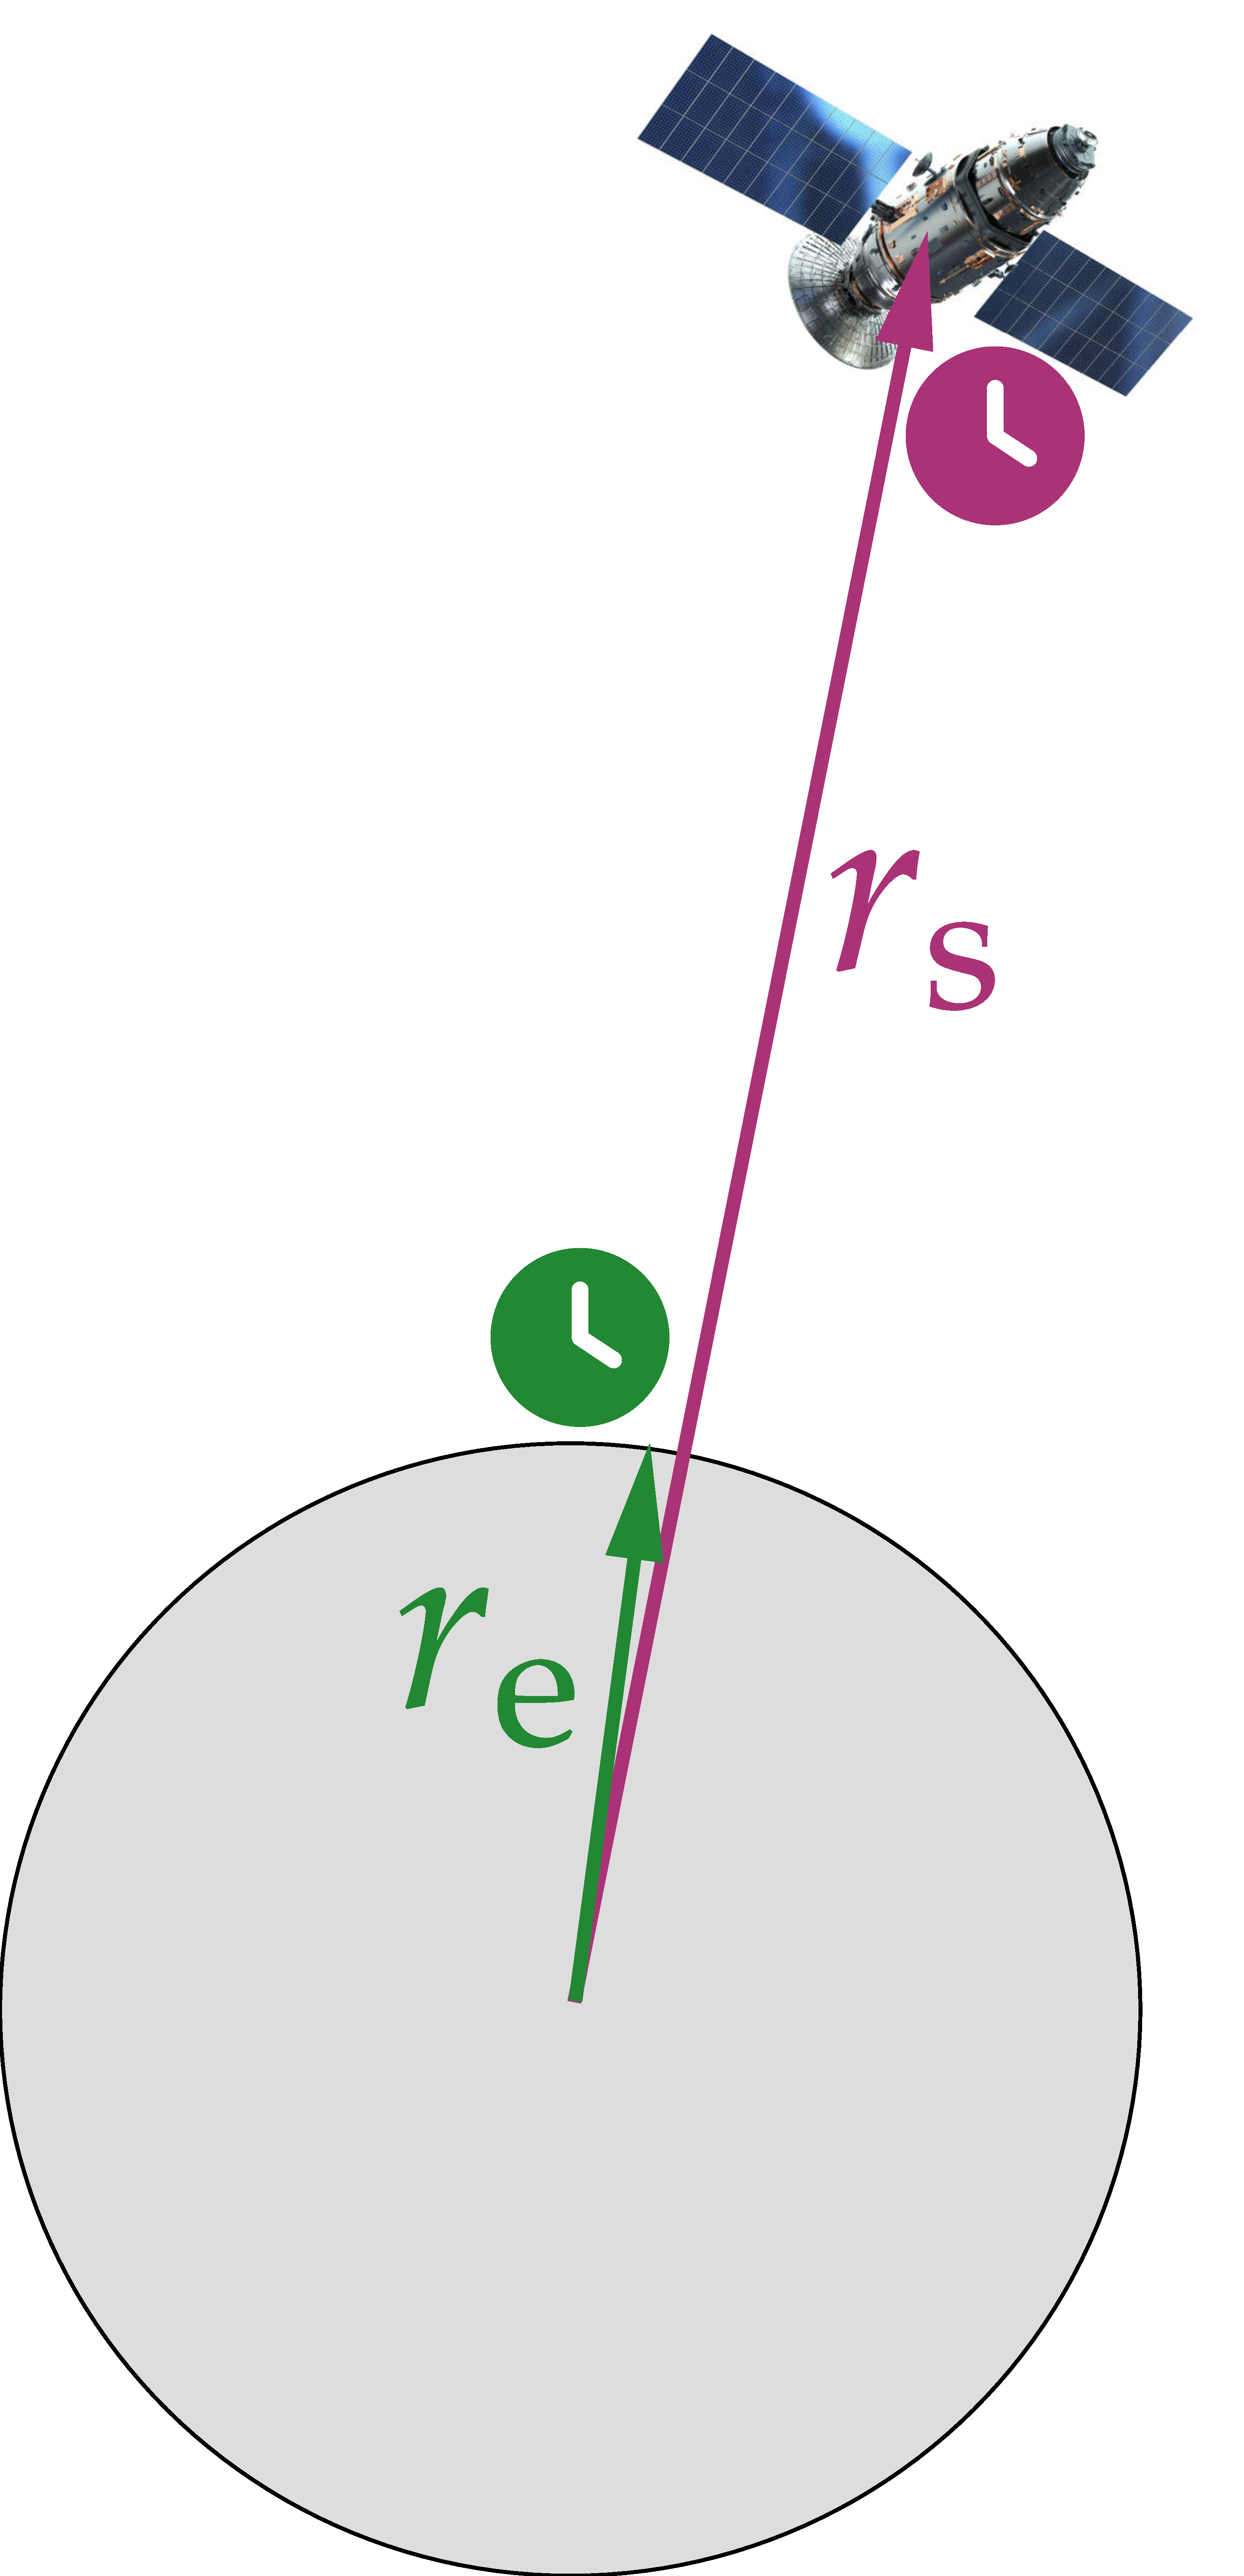
\includegraphics[align=t,width=0.75\linewidth]{images/re_rs.pdf}
% }
%   Consider a clock at rest on the Earth's surface, at a distance $\color{green}r_{\text{e}}$ from the Earth's centre; and a clock on a satellite, for instance a GPS satellite or the \furl{https://www.nasa.gov/international-space-station/}{International Space Station}, right above the first clock, at a distance $\color{red}r_{\text{s}}$ from the Earth's centre. An observer by the clock on Earth measuring a time lapse $\Dt_{\text{e}}$ will see the clock on the satellite has having run for a time lapse $\Dt_{\text{s}}$, and vice versa (note that this \enquote{vice versa} only holds in this specific situation!). The relation between two time lapses is approximately given by
% \begin{equation*}
%   \frac{\Dt_{\text{s}}}{\Dt_{\text{e}}} =
%   \frac{
%     \sqrt{1-\frac{G}{c^{2}}\frac{M}{r_{e}}}
%   }{
%     \sqrt{1-\frac{G}{c^{2}}\frac{M}{r_{s}}}
%   }
% \end{equation*}
% where $G\approx\qty{6.7e-11}{m^{3}/(kg.s^{2})}$, $c=\qty{3.0e8}{m/s}$, and the Earth's mass $M=\qty{6.0e24}{kg}$.
%
%
% \begin{enumerate}[exerc]
% \item Take the case of a GPS satellite, with $r_{\text{e}}=\qty{6.4e6}{m}$ and $r_{\text{s}}=\qty{2.6e7}{m}$ (\furl{https://www.nasa.gov/directorates/somd/space-communications-navigation-program/gps/}{NASA data}). If you, on the ground, measure a time lapse of $\Dt_{\text{e}}=\qty{10}{years}$, what's the difference, in seconds, with the time lapse $\Dt_{\text{s}}$ you see on the satellite?
%
% \item If the time lapses are large compared with the time needed to go from ground to orbit or vice versa, then $\Dt_{\text{s}}/\Dt_{\text{e}}$ is also the ratio between the real \emph{ageing} of a person who's been in orbit and one who's been on the ground, when they meet again.
%
%   Now consider the case with a black hole instead of Earth. The formula above still apply approximately.
%
%   In the movie \furl{https://www.imdb.com/title/tt0816692/}{\emph{Interstellar}}, two
%   astronauts go on Miller's planet, at a distance $r_{\text{e}}$ from the black hole Gargantua, and stay there for \qty{3}{hours}, leaving one astronaut in orbit at a distance $r_{\text{s}}\approx \infty$ (the distance is large enough that it can be approximated as infinity). When they meet again, the latter astronaut has aged \emph{23\;years}.
% \sidepar{\footnotesize\centering%
% \vspace{-10em}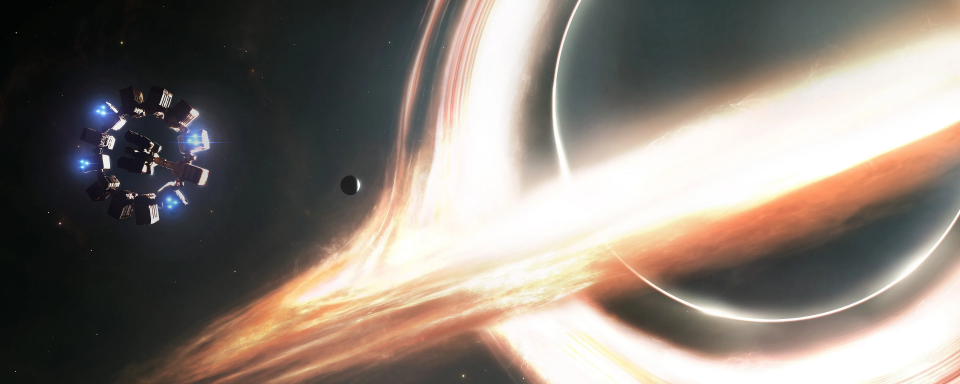
\includegraphics[width=\linewidth]{images/gargantua.png}
% }
%
%   Given that Gargantua's mass is $M=\qty{2.0e38}{kg}$, calculate the distance $r_{\text{e}}$ of Miller's planet from the black hole.
% \end{enumerate}
%
%
%
% \end{subappendices}





\printpagenotes*
\cleartooddpage
\chapter{Main physical quantities}
\label{cha:stuff}

\epigraph{For Euler, clarity was the hallmark of truth. \textelp{} To him we owe also the brilliant imagination of the internal pressure in generality
  % , the pressure field as equipollent to the action of the fluid outside any imaginary closed diaphragm upon that within.
  \textelp{} I remark upon it in emphasis of the role of imagination and the importance of quantities which can only be thought of and cannot in themselves be measured.}{C. A. Truesdell \cites*{truesdell1956d}}

% \epigraph{if the skill of the mathematician has enabled the experimentalist to see that the quantities which he has measured are connected by necessary relations, the discoveries of physics have revealed to the mathematician new forms of quantities which he could never have imagined for himself.}{J. Clerk Maxwell \cites*{maxwell1870}}


\section[Seven primitive quantities]{Seven primitive quantities}
\label{sec:stuff}

The discovery, formulation, and use of \autoref{sec:phys_laws0}{physical laws} requires us to look at the world from a more abstract and quantifiable point of view.
As \autoref{sec:primitives}{previously discussed}, we shall achieve this by interpreting all physical phenomena around and within us in terms of time \amp\ space, which we have studied in \chap~\ref{cha:time_space}, and of seven physical quantities:
\begin{definition}{Seven primitive quantities}
  \begin{minipage}[c]{0.49\linewidth}
    \begin{center}\bfseries
      matter
      \\ electric charge
      \\ magnetic flux
    \end{center}
  \end{minipage}\hfill
  \begin{minipage}[c]{0.49\linewidth}
    \begin{center}\bfseries
      \energym
      \\ momentum
      \\ angular momentum
      \\[2\jot] entropy
    \end{center}
  \end{minipage}
\end{definition}
% Technically they are called \emph{fields}, for reasons we shall shortly see.
We take these seven quantities as primitive, and shall build our physical laws upon them. Each of these seven quantities satisfies a universal physical law; other physical laws express relationships among these quantities.

Recall that \autoref{sec:primitives}{primitive quantities cannot be defined}: we can only try to understand them intuitively. This is the goal of present chapter: to make a brief acquaintance with the seven primitive quantities and with some% additional ones.

\section{Two basic properties}
\label{sec:sevenquantities_properties}

Our seven primitive quantities have two basic properties in common:

\subsection{First property: three measurements}
\label{sec:sevenquantities_property1}

For each quantity -- with a slight change for the magnetic flux -- we can ask about or measure three kinds of amount:
\begin{definition}{Three basic measurements of the seven quantities}\label{def:volumecontent}
  \begin{enumerate}[label={M\arabic*}.,leftmargin=3em]
  \item\label{item:meas1}How much of this quantity is \textbf{contained} in a particular three-dimensional region of space at a particular time instant?

  \item\label{item:meas2a}How much of this quantity \textbf{flows} through a particular two-dimensional surface, in a given direction, during a particular time lapse?

  \item\label{item:meas3a}How much of this quantity is \textbf{produced} in a particular three-dimensional region of space during a particular time lapse?
  \end{enumerate}
\end{definition}
%
\marginpar{\vspace{-12\baselineskip}\footnotesize\centering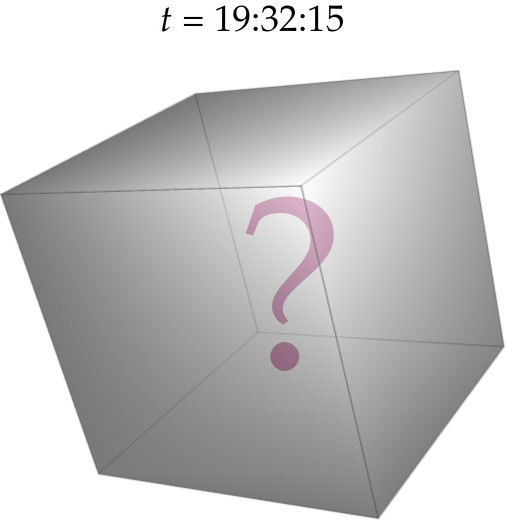
\includegraphics[width=\linewidth]{images/howmuch_volume.jpg}%
\\[\jot]\flushleftright\color{mpcolor}%
For six main quantities we can ask: how much of it is in a given volume, at a given time?

\mbox{} \\[2\baselineskip]\centering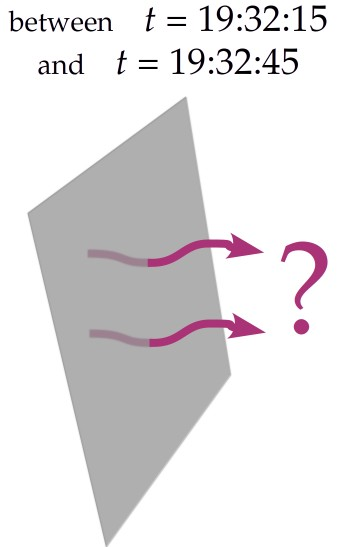
\includegraphics[width=0.7\linewidth]{images/howmuch_surface.jpg}%
\\[\jot]\footnotesize\flushleftright\color{mpcolor}%
For six main quantities we can ask: how much of it is flowing through a given surface in a given direction, during a given time lapse?%
}%
We can ask these questions for any region of space, any time instant, any time lapse. The regions of space can be moving and deforming. The results of the three measurements above are scalars for scalar quantities, and vectors for vector quantities.
% This number depends only on the chosen region, surfaces, and times.

Questions~\ref{item:meas2a} and \ref{item:meas3a} can also be asked in a different way. Consider a very short lapse of time, and divide the net flow and the net production by that lapse of time. This way we have an alternative form of the second and third measurements, as flow or production divided by time:
\begin{definition}{Second and third measurement: new version}\label{def:fluxsupply}
  \begin{enumerate}[label={M\arabic*b}.,start=2,leftmargin=3em]
  % \item\label{item:meas1}How much of this quantity is \textbf{contained} in a particular three-dimensional region of space at a particular time instant?

  \item At which rate is this quantity flowing through a particular two-dimensional surface in a given direction, at a particular time instant?

    We call this the \textbf{flux} of the quantity through that surface.

  \item At which rate is this quantity being produced in a particular three-dimensional region of space, at a particular time instant?

    We call this the \textbf{supply} or \textbf{source} of the quantity in that region.
  \end{enumerate}
\end{definition}

In the case of magnetic flux we can ask the three questions above in 2 and 1 dimensions, rather than in 3 and 2 dimensions, as we shall see in \chap~\ref{cha:cons_magneticflux}.

% \subsection{Second property: extensivity}
% \label{sec:sevenquantities_property2}

The second property common to all seven quantities tells how the measurements above combine for several regions of space and several surfaces:
\begin{definition}{Extensivity or additivity}\label{def:extensivity}
\begin{itemize}[leftmargin=17.62pt]
\item If we consider two or more non-overlapping volumes, the amount of quantity contained in the total volume is equal to the sum of the amounts contained in the individual volumes.

\item If we consider two or more non-overlapping surfaces, the amount of quantity flowing through the total surface is equal to the sum of the amounts flowing through the individual surfaces.

\item If we consider two or more non-overlapping volumes, the amount of quantity produced in the total volume is equal to the sum of the amounts produced in the individual volumes.
  \end{itemize}

We say that each of the seven quantities is \textbf{extensive} or \textbf{additive}.
\end{definition}


% We shall later see that analogous properties hold for the magnetic flux, the only difference being that instead of holding in 3 and 2 dimensions, they hold in 2 and 1 dimensions.

\medskip

The basic measurements above cannot in general be made, and do not even make sense, for some other quantities. For instance, we cannot ask \enquote{what's the total amount of temperature in this region?}, or \enquote{how much velocity is flowing through this surface?}.

\medskip

Thanks to the two properties above, each of the seven quantities can be intuitively visualized as some kind of \enquote{stuff} that fills regions of space or flows through surfaces. This visualization is useful, but also comes with some warnings which we shall discuss later.
% But don't take the word \enquote*{stuff} too literally: I don't necessarily mean concrete objects like a ball, or substances like water.

% For each quantity, we can speak of its \emph{density}, in relation to the question \enquote{how much of it is in a particular region?}; and of its \emph{flux}, in relation to the question \enquote{how much of it flows through a surface during some time?}. The density tells us how much quantity there's in a unit of volume. The flux tells us how much quantity is flowing through a unit of surface in a unit of time. Density and flux can change from spacetime point to spacetime point. We shall discuss them more in detail for each quantity later on. One important aspect to keep in mind is that \emph{the density and flux of each quantity depend on the coordinate system}.

\medskip

What's remarkable about matter, electric charge, magnetic flux, \energym, momentum, angular momentum, and entropy, is that \emph{they are common to all our main physical theories}, approximate or not: from Newtonian mechanics to General Relativity and Quantum Theory; from subatomic scales to cosmological scales. And in all these theories they possess the two basic properties discussed above. The mathematical characterization of these quantities can be slightly different depending on the physical theory and spatial or temporal resolution. For example, in quantum theory a quantity is mathematically represented by a so-called \enquote*{operator}. And on molecular scales, entropy has a meaning connected with probability theory. Yet, these seven quantities are universal in our present way of doing physics and of describing and understanding physical phenomena all around and within us.

% \begin{critique}
%   \emph{Wait! what about \emph{force}? isn't this a primitive quantity? or maybe it isn't included because it's defined as mass${}\times{}$acceleration?}
%
%   \smallskip
%
% We'll see that \emph{force} is defined as momentum flux; but that in general isn't mass${}\times{}$acceleration.
% \end{critique}

Let us make a first acquaintance with these seven quantities. The discussion that follows is meant as an introduction. We shall repeat and say more about each quantity in later chapters.
% %
% \marginpar{\vspace{-6\baselineskip}\footnotesize\centering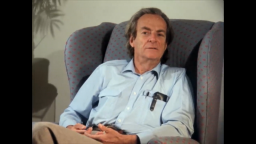
\includegraphics[width=\linewidth]{images/feynman_why2.png}%
% \\[\jot]\flushleftright\color{mpcolor}%
% Richard Feynman explains the difficulty of \enquote{why} questions in a \furl{https://www.youtube.com/watch?v=nYg6jzotiAc&t=893s}{funny and insightful video}.%
% }%
But \autoref{sec:primitives}{remember} that it is very difficult, if not impossible, to answer questions like \enquote{what is \emph{really} the quantity\textellipsis?}.

\section{Matter}
\label{sec:intro_matter}

\marginpar{\vspace{2\baselineskip}\footnotesize\centering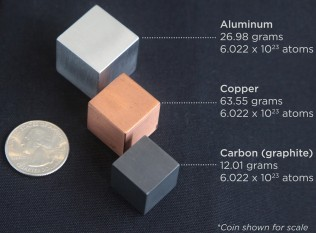
\includegraphics[width=\linewidth]{images/mole.jpg}%
\\[\jot]\flushleftright\color{mpcolor}%
One mole of different substances (\furl{https://www.nist.gov/image/moleedit2jpg}{image: NIST}).%
}%
\begin{definition}{Matter: units and notation}
  Matter, which includes \furl{https://doi.org/10.1351/goldbook.A00297}{\emph{amount of substance}} in chemistry, is a \emph{scalar} quantity. The unit for the amount of matter is the \furl{https://www.nist.gov/si-redefinition/redefining-mole}{\emph{mole}} \unit{mol}; the unit for matter flux and supply is \emph{mole per second} \unit{mol/s}. In statistical mechanics and particle physics, matter is often simply counted and thus measured in dimensionless units, rather than in moles.

  \smallskip

The amount of matter in a volume is usually denoted $\yN$. The flux of matter through a surface is denoted $\yJ$; and supply of matter in a volume, $\ya$. In chemistry we usually specify what kind of matter we are speaking about, writing for instance $\yN_{\mathrm{Ca}}=\qty{5.3}{mol}$, to indicate an amount of $\qty{5.3}{mol}$ of \furl{https://pubchem.ncbi.nlm.nih.gov/element/Calcium}{calcium} atoms.
\end{definition}


Matter is probably the easiest quantity to grasp intuitively: it is what we ordinarily call \enquote{stuff}. % It is called \furl{https://doi.org/10.1351/goldbook.C01039}{\emph{chemical substance}} in chemistry, and \emph{baryons} and \emph{leptons} in particle physics.
It is usually classified into several kinds. The classification depends on the physical phenomena and theory one works with. A building engineer, for instance, could classify \enquote{matter} into different kinds of \emph{materials} -- such as wood, concrete, steel, sand, plastic, and so on -- keeping track of the amount of each material in different regions of space, its movement, its rate of production and transformation. Each material has different physical properties.

A chemist could classify matter into different \emph{substances} -- such as water, hydrogen, oxygen, carbon dioxide, and so on -- again keeping track of their amounts, movements, production. According to this classification, the \enquote{materials} of the building engineer would be mixtures of the different substances. But note that there is no clear boundary between one classification and the other.

A chemist could also classify matter into different kinds of \emph{atoms} -- such as \furl{https://pubchem.ncbi.nlm.nih.gov/element/Hydrogen}{hydrogen}, \furl{https://pubchem.ncbi.nlm.nih.gov/element/Helium}{helium}, \furl{https://pubchem.ncbi.nlm.nih.gov/element/Lithium}{lithium}, and the other kinds that appear in the \furl{https://iupac.org/what-we-do/periodic-table-of-elements/}{periodic table} -- and seeing substances and materials as combinations of these different atomic kinds of matter. This classification is special because these different kinds have, at least approximately, the property of being \autoref{sec:balance_intro}{conserved}: their amounts in a container or in a region of space can only change if these kinds are entering through an opening in the container or through the boundary of the region of space. In other words, they cannot be created or destroyed. This conservation property is only approximate, however. \furl{https://www.ciaaw.org/radioactive-elements.htm}{Radioactive atoms} can transmute from one kind to another. This possibility is crucial and must be taken into account in phenomena involving \furl{https://www.iaea.org/newscenter/news/what-are-radioactive-sources}{radioactivity}
% \url{https://www.britannica.com/science/radioactivity}
and \furl{https://www.iaea.org/newscenter/news/what-is-nuclear-energy-the-science-of-nuclear-power}{nuclear \energym}.

A chemist or a particle physicist may classify matter into fewer different kinds: protons, neutrons, electrons, anti-protons, anti-neutrons, anti-electrons (also called \emph{positrons}), seeing the different atomic kinds as being made of these six basic ones. These kinds may be conserved even when kinds of atoms are not.

But a nuclear or particle physicist knows that the conservation properties of the six kinds above is also only approximate, and there are also other kinds, produced only in special circumstances.

We therefore go down into more and more subtle classifications. This kind of research is still open, but it seems that the total amount of \furl{http://hyperphysics.phy-astr.gsu.edu/hbase/Particles/hadron.html\#c6}{\emph{baryonic}},
% \url{https://www.britannica.com/science/baryon}
(including protons and neutrons) and \furl{http://hyperphysics.phy-astr.gsu.edu/hbase/Particles/lepton.html\#c1}{\emph{leptonic}} (including electrons) matter is always conserved.
% \url{https://www.britannica.com/science/lepton},

\medskip

According to the definition of matter that we're adopting, the total amount of some kind of matter in a region can in principle be \emph{negative}. A negative amount simply denotes the presence of \furl{https://www.britannica.com/science/antimatter}{anti-matter}. Anti-matter appears in small amounts in everyday life, for example in connection with common radioactivity processes. It is also created and used in medicine, in \furl{https://www.britannica.com/topic/positron-emission-tomography}{positron-emission tomography (PET)} scans. In ordinary chemical applications, however, all amounts of matter within a region are usually positive or zero.
%
\marginpar{\vspace{-8\baselineskip}\footnotesize\centering%
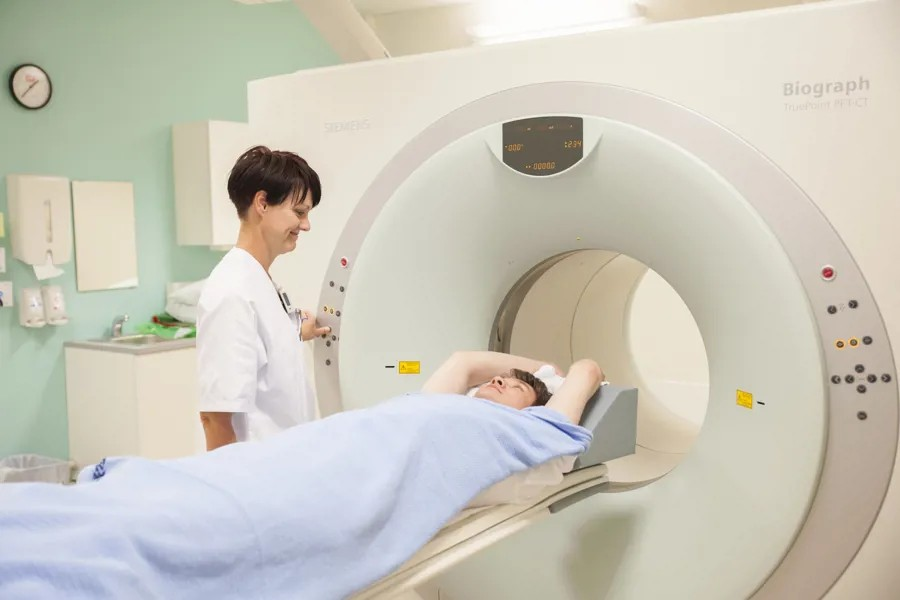
\includegraphics[width=\linewidth]{images/pet_scan_bergen.jpg}%
\\[\jot]\footnotesize\flushleftright\color{mpcolor}%
In positron-emission tomography there is creation of amounts of matter (leptonic matter) that can be considered negative: their \emph{lepton number} is negative (\furl{https://www.helse-bergen.no/avdelinger/radiologisk-avdeling/senter-for-nukleermedisin-og-pet/tilvising-til-pet}{image: Helse Bergen}).%
}%

\medskip

Why do we need to worry about how matter gets classified depending on the application? Because for describing a physical system and predicting its behaviour we usually have to use at least one physical law \emph{for each kind of matter}. So the more kinds of matter we have to keep track of, the more equations we will have.




\begin{warning}[Ambiguity of the term \enquote*{matter}]
In these notes we use the term \enquote*{matter} in the generic sense discussed above. But be aware that in some disciplines this term may have a much more specialized and slightly different meaning. It may \emph{not} even be used at all. In chemical applications, for instance, one typically speaks specifically of \enquote*{compounds}, \enquote*{mixtures}, \enquote*{substances}, \enquote*{elements}, rather than \enquote*{matter}. A particle physicists speaks of \emph{matter} and \emph{anti-matter}, but in the present notes the term \enquote*{matter} refers to both.
\end{warning}


% In these notes we shall usually not consider distinctions between different kinds of matter, making some exceptions for discussions about chemical reactions and nuclear phenomena.

% There are different kinds of matter The distinction into different kinds depends on the physical theory. In most everyday situations, the distinction corresponds to different \furl{https://doi.org/10.1351/goldbook.C01022}{chemical elements}, and each satisfies its own balance. These balances are the basis of \furl{https://doi.org/10.1351/goldbook.S06026}{stoichiometry}. If we observe phenomena like nuclear fission or fusion, however, we notice that the balances of chemical elements are not really satisfied. With such phenomena we make a different distinction of types of matter, for instance \emph{baryons} and \emph{leptons}, and each satisfies again its own balance. It is unclear whether these balances might be broken in other physical phenomena on smaller scales. In these notes we shall usually consider chemical elements as the different kinds of matter, making some exceptions in discussion of nuclear phenomena.

\begin{warning}[Matter is different from \masse]
  It is important to clearly distinguish \emph{matter} from \emph{\masse}. Mass-energy can be considered a property of matter, but the two are different. In nuclear reactions, for instance, the \masse\ of some amount of matter may change, while the amount of matter stays the same.

  \smallskip

  As far as we know, the total amount of \masse\ associated with an amount of matter is always positive, whether the amount of matter is positive or negative (antimatter). This is the reason why antimatter \enquote{falls downward} just like positive matter, a fact that has been experimentally confirmed: see \cites{andersonetal2023}.
\end{warning}

%
\marginpar{\vspace{3\baselineskip}\footnotesize\centering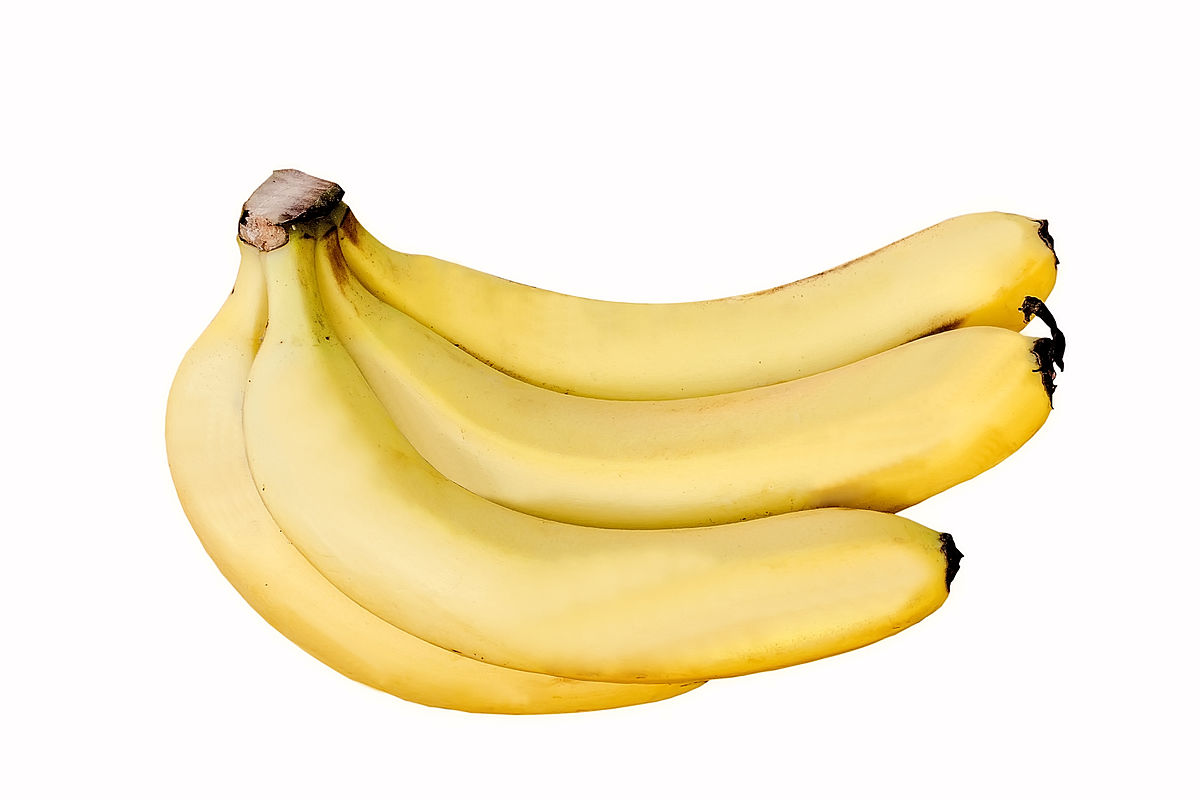
\includegraphics[width=\linewidth]{images/banana.jpg}%
\\\flushleftright\color{mpcolor}How many positrons do bananas produce?%
}%
\begin{exercise}
  According to statements on \furl{https://www.symmetrymagazine.org/2009/07/23/antimatter-from-bananas}{symmetrymagazine.org} and \furl{https://www.quantumdiaries.org/2009/07/21/positrons-from-bananas/}{quantumdiaries.org},
  \begin{quote}
    The average banana (rich in potassium) produces a positron roughly once every 75 minutes.
  \end{quote}
  Unfortunately the original site where the this statement was discussed, and the corresponding calculation made, seems not to exist anymore.

\begin{enumerate}[exerc]
\item Do a little research and find out whether this statement is true.
\item From your research, approximately quantify the flux of positrons around an ordinary banana, expressing it in \unit{particles/s}.
\end{enumerate}
\end{exercise}



\section{Electric charge}
\label{sec:intro_charge}

\begin{definition}{Electric charge: units and notation}
  Electric charge is a \emph{scalar} quantity. The unit for the amount of electric-charge is the \furl{https://doi.org/10.1351/goldbook.C01365}{\emph{coulomb}} \unit{C}. The flux of electric charge is called \emph{electric current}, its unit is the \furl{https://www.nist.gov/si-redefinition/ampere-introduction}{\emph{ampere}} $\unit{A} = \unit{C/s}$.
\end{definition}

\mynotew{To be completed in a later version}



\section{Magnetic flux}
\label{sec:intro_magneticflux}

%
\marginpar{\vspace{2\baselineskip}\footnotesize\centering%
%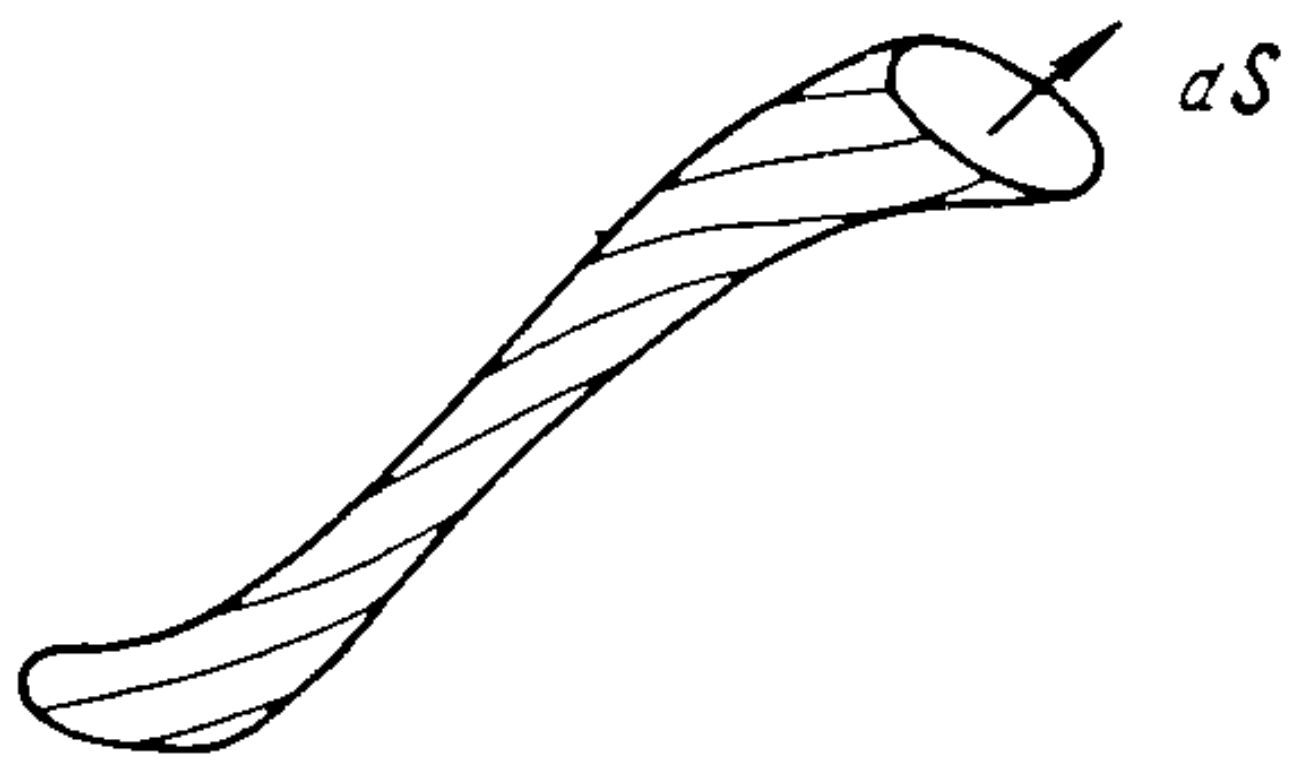
\includegraphics[align=t,width=\linewidth]{images/magnflux1.png}
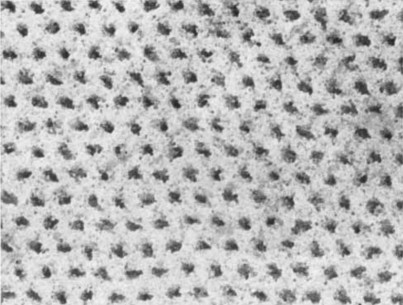
\includegraphics[width=\linewidth]{images/magnetic-flux_lines.jpg}%
\\[\jot]\flushleftright\color{mpcolor}\enquote{\emph{%
magnetic-flux lines emerging from the surface of a Type~II superconductor}}\sourceatright{\cites{essmannetal1971}}%
}%
\begin{definition}{Magnetic flux: units and notation}
  Magnetic flux is a \emph{scalar} quantity. The unit for magnetic flux is the \furl{https://doi.org/10.1351/goldbook.W06666}{\emph{weber}} \unit{Wb}. The \enquote{flux} of magnetic flux is called \emph{electric potential difference} or \emph{electric tension}; its unit is the \furl{https://doi.org/10.1351/goldbook.V06634}{\emph{volt}} $\unit{V} = \unit{Wb/s}$.

  \smallskip

  The magnetic flux is usually calculated by means of a \emph{vector} quantity called \emph{magnetic flux density}; its unit is the \furl{https://doi.org/10.1351/goldbook.T06283}{\emph{tesla}} $\unit{T} = \unit{Wb/m^{2}}$.

  \smallskip

  The electric potential difference is usually calculated by means of a \emph{vector} quantity called \emph{electric field strength}; its unit is the \emph{volt per metre} (\unit{V/m}).
\end{definition}

As we shall see in more detail in \chap~\ref{cha:cons_magneticflux}, magnetic flux differs from the other six main quantities in that it answers the two \enquote{how much?} questions \emph{in one lower dimension}: \enquote{How much magnetic flux is in this surface?} and \enquote{How much magnetic flux crosses this line in the unit of time?}. It also requires a slightly different notion of orientation of a surface. The \enquote{flux of magnetic flux}, or \emph{electric potential difference}, is therefore a flow connected to a line.


\marginpar{\vspace{-4\baselineskip}\footnotesize\centering%
%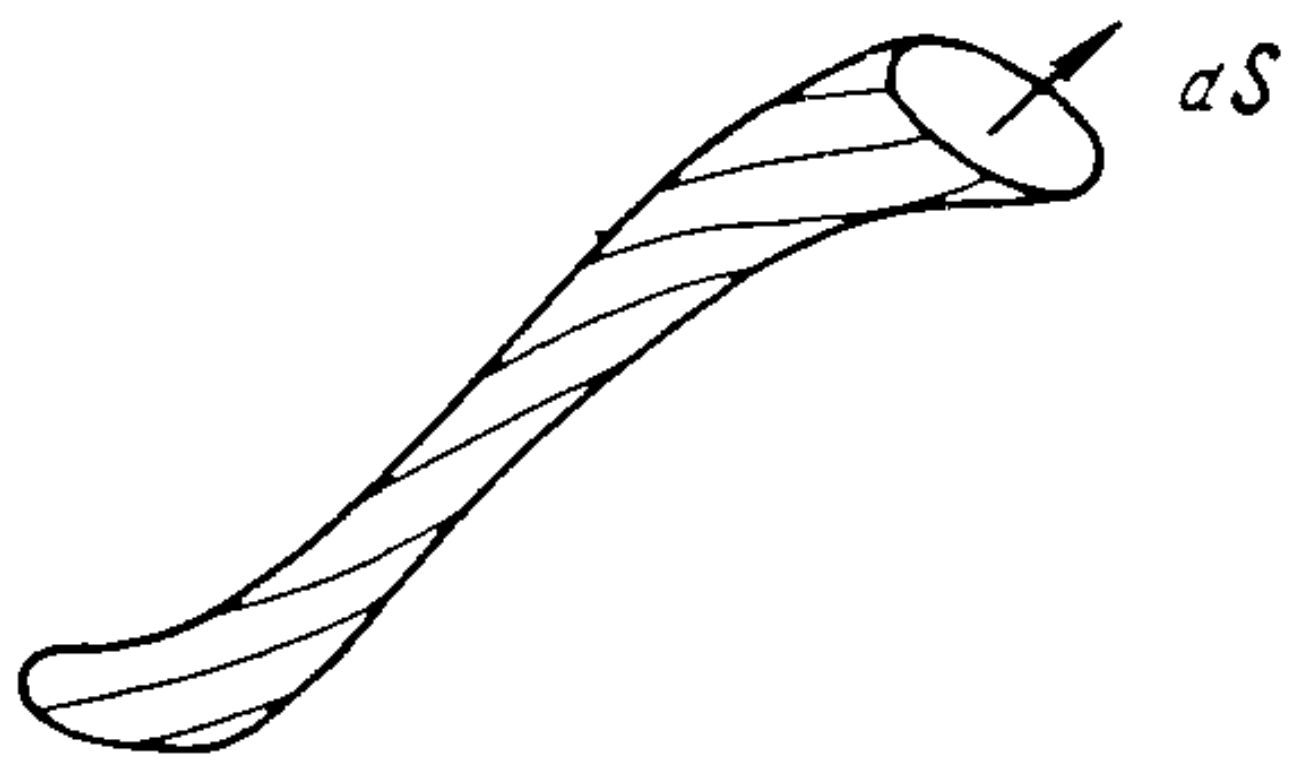
\includegraphics[align=t,width=\linewidth]{images/magnflux1.png}
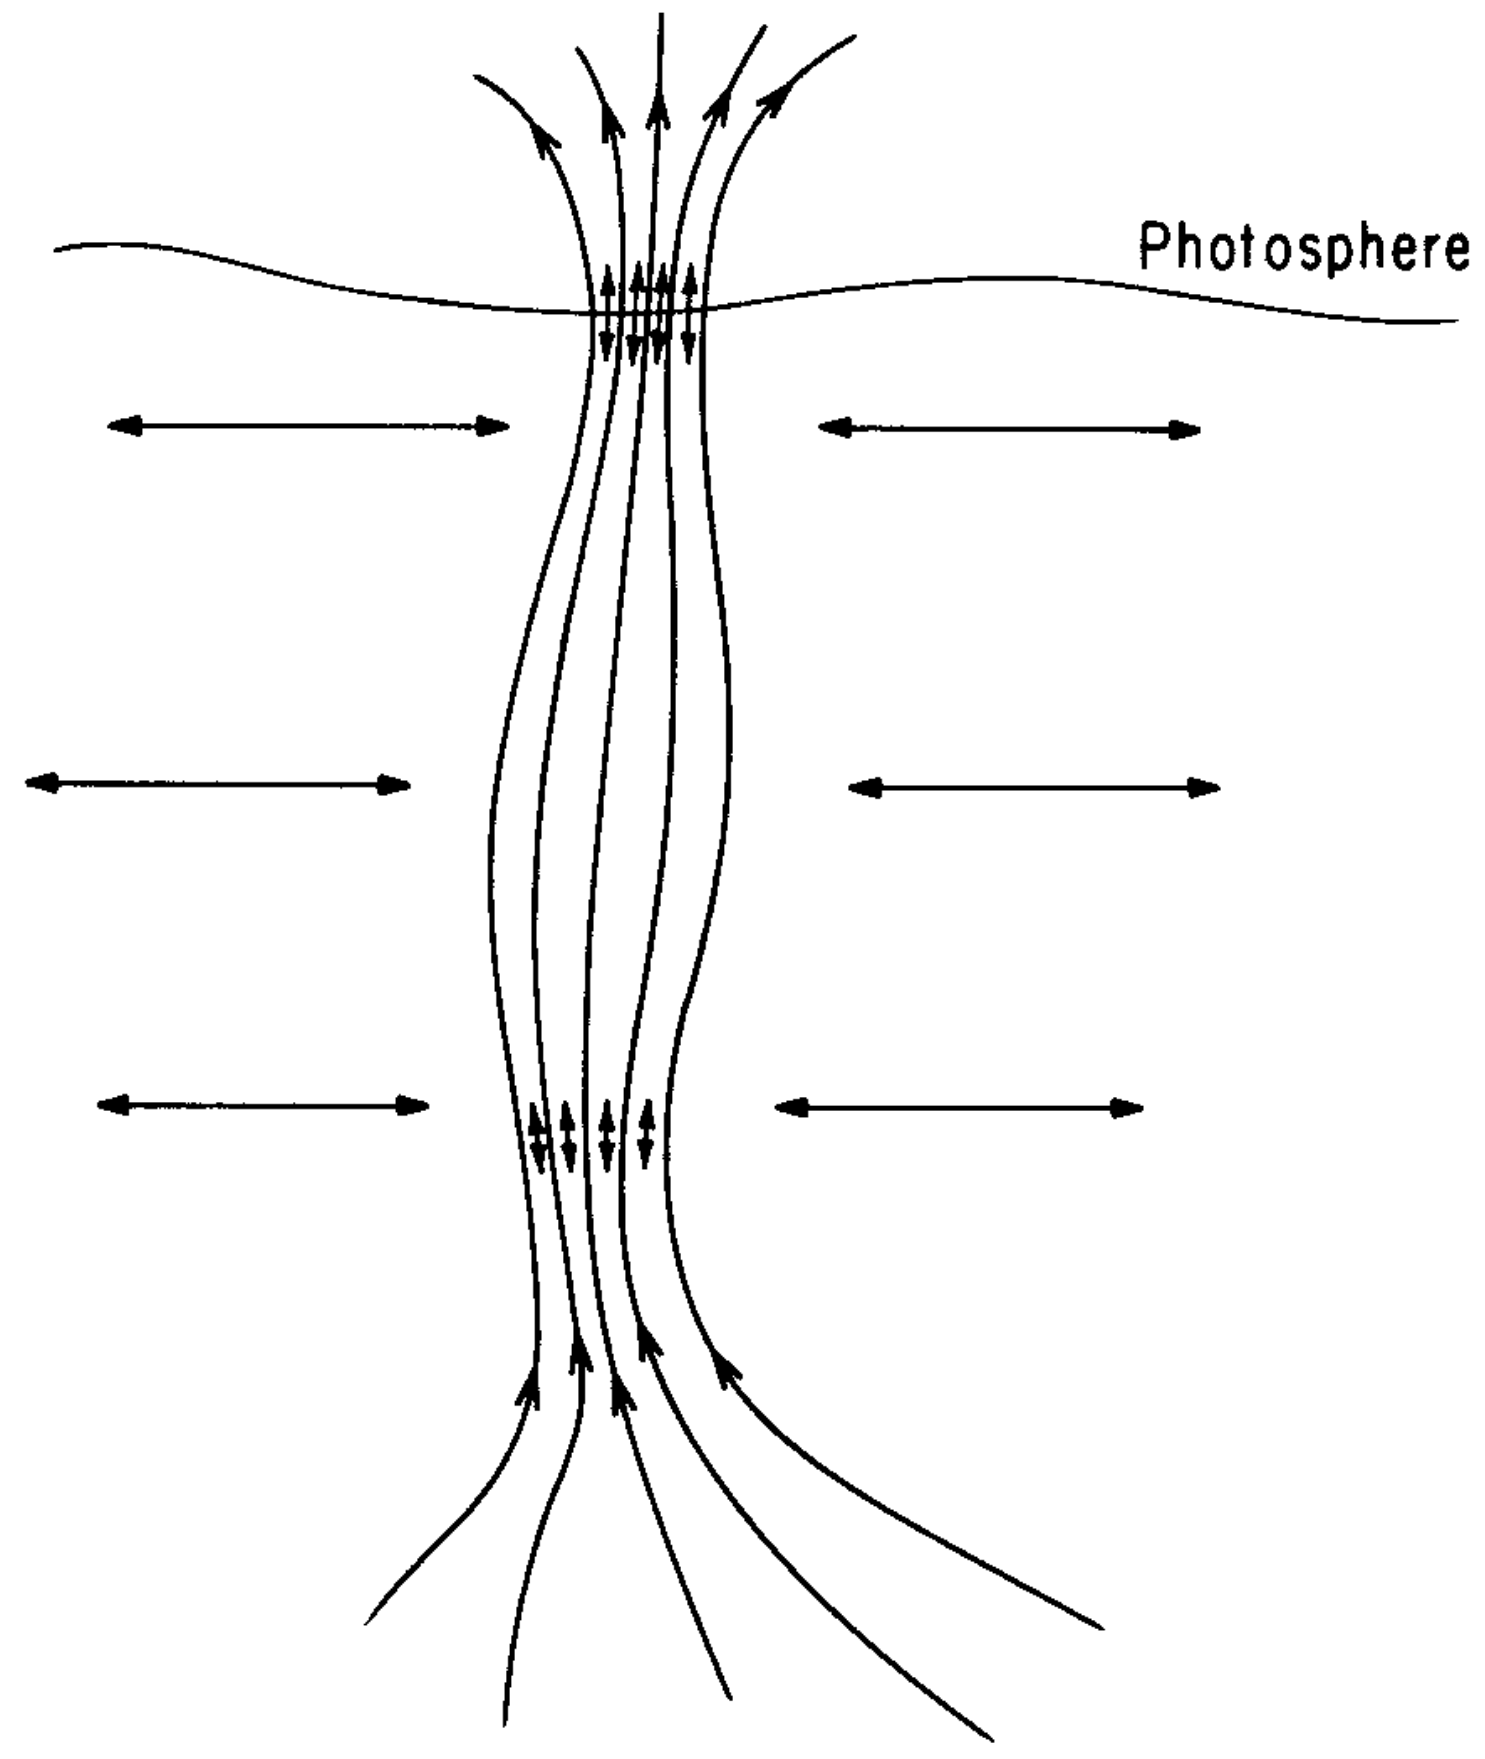
\includegraphics[width=\linewidth]{images/magnflux2.png}%
\\[\jot]\flushleftright\color{mpcolor}\enquote{\emph{%
sketch of the magnetic lines of force in a magnetic filament extending up through the photosphere.}}\sourceatright{\cites{parker1974b}}%
}
The magnetic flux density and the electric field strength together are usually called \enquote{electromagnetic field}, which is therefore commonly represented by two vectors associated to each point in space. But it can also be interpreted and visualized as a collection of spinning magnetic tubes or lines, either closed or extending indefinitely, which move around. This visualization is somewhat analogous to how we visualize matter and charge, as moving blobs or points, but with one more dimension. This interpretation goes back to Faraday \parencites*{faraday1846}, Maxwell \parencites*{maxwell1855b}, and later Dirac \parencites*{dirac1955} among others, and today is conveniently used in some fields such as \furl{https://doi.org/10.1093/acrefore/9780190871994.013.21}{solar physics}, for example to study \furl{https://spaceplace.nasa.gov/solar-activity/}{sunspots} (see Ryutova \cites*{ryutova2015_r2018}). In particular situations, for example in some superconductors subjected to external magnetic fields, the magnetic-flux lines can literally be seen and even tracked as they move around (see previous side figure).

\mynotew{To be completed in a later version}

% \section{Energy-mass, momentum, and related quantities}
% \label{sec:energy-mass-momentum}
% 
% \emph{Energy}, \emph{mass}, \emph{momentum}, and related quantities like \emph{angular momentum}, \emph{force}, \emph{power}, \emph{heat}, \emph{torque} are quite subtle, have some peculiar characteristics, and require some time and exercise to be fully learned. The difficulties in learning them arise for several reasons, partly physical, partly sociological:
% \begin{itemize}
% \item From general relativity we know that there aren't clear-cut distinctions among these quantities. They are all parts of one, more complicated quantity.
% \item The distinctions among these quantities depend on the coordinate system.
% \item Different scientists adopt different and sometimes slightly incompatible definitions of these quantities.
% \item Today our understanding of some of these quantities is different from the one we had in the past, but much inertia and tradition in their conception and teaching still remain.
% \end{itemize}
% 
% 
% 
% From general relativity we know that there aren't clear-cut distinctions among these quantities. There is actually only one quantity, called \emph{energy-momentum tensor}. This quantity is not a scalar: similarly to what happens with position or velocity, it cannot be expressed by a single number; but it is more complicated than a vector. It can be represented as a 4-by-4 matrix with 16 entries. Energy, momentum, force, and several other quantities are part of 

\section{Energy-mass}
\label{sec:intro_energy}

%
\marginpar{\vspace{2\baselineskip}\footnotesize\centering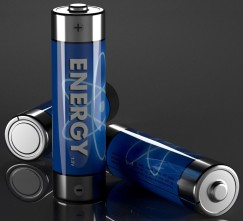
\includegraphics[width=0.75\linewidth]{images/AAbattery.jpg}%
\\[\jot]\flushleftright\color{mpcolor}%
The \emph{chemical} \energym\ content in an ordinary AA battery is around \qty{10000}{J}. The \emph{total} \energym\ content, including rest \energym, is around \qty{e15}{J}.
}%
\begin{definition}{Energy-mass: units and notation}
  Energy is a \emph{scalar} quantity. The unit for the amount of energy is the \emph{joule} \unit{J}; the unit for energy flux and supply is \emph{joule per second} \unit{J/s}, also called \emph{watt} $\unit{W} = \unit{J/s}$.

  \smallskip

  Equivalently we can speak of mass. The unit for the amount of mass is the \furl{https://doi.org/10.1351/goldbook.K03391}{\emph{kilogram}} \unit{kg}; the unit for mass flux and supply is \emph{kilogram per second} \unit{kg/s}.

  \smallskip

  The amount of energy in a volume is usually denoted $\yE$, or $\ym$ if we describe it as mass. % Internal energy is denoted $\yU$, kinetic energy $\yEk$, potential energy $\yEp$.
  The flux of total energy through a surface is denoted $\yH$; and supply in a volume, $\yR$.% ; the flux in the form of heat, by $\yQ$; and in the form of work, by $\yW$.
\end{definition}


The notion of energy is extremely important today, and central in many world-wide discussions and worries -- think of today's \enquote{energy crisis}, the need for \enquote{renewable energy}, and so on. It is somewhat funny that despite its importance it's actually difficult to answer \enquote*{what \emph{is} energy, really?}. Often we speak about energy as something that \enquote{flows}, is \enquote{transported}, \enquote{converted}, \enquote{stored}, and similar visualizations. This intuition will be enough in these notes. The notion of \emph{mass} is also very intuitive in our everyday life; we associate it with the \enquote{resistance} we feel when setting objects into motion, or with the weight of objects.
% relativity says that there's a strong connection between these two associations.

From Relativity Theory -- and experimentally -- we know that \emph{energy and mass are the same quantity}, and in these notes we shall emphasize this experimental fact.


\subsection{Energy is mass, mass is energy}
\label{sec:mass_is_energy}

Let's see some examples of why it is impossible to make a distinction between energy and mass. The following examples have been simplified in some of their aspects, but their main point is valid.

\paragraph{Heated gas.}

Imagine we have a box with a given amount of gas, say \qty{1}{mol} of oxygen molecules. Using an extremely precise weighing scale, we observe that the mass of the gas is, say, exactly
\begin{equation*}
  \qty{0.031999540000000000}{kg} \ .
\end{equation*}
Now we heat the gas, providing \qty{60}{J} of energy, while making sure that not a single molecule of oxygen gets in or out of the box. The temperature of the gas increases by around \qty{3}{K}. We actually observe that the weight measured by the scale increases while we heat the gas, reaching the new value
% cp= 29.4 J/mol/K  cv=21.1
\begin{equation*}
  \qty{0.031999540000000668}{kg} \ .
\end{equation*}
Clearly the mass has increased, but no molecules were added! The additional mass is the \qty{60}{J} of energy that we provided to the gas by heating. Energy has weight, energy is mass.

% Some texts say that \enquote{mass is a form of energy}, but that's incorrect: mass \emph{is} energy, and energy in all its possible forms \emph{is} mass.

\paragraph{Stretched or moving rubber band.}

%
\marginpar{\vspace{-4\baselineskip}\footnotesize\centering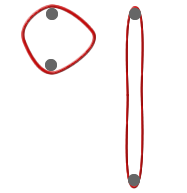
\includegraphics[width=\linewidth]{images/rubberbands.png}%
\\[\jot]\flushleftright\color{mpcolor}When we stretch a rubber band, its mass increases slightly -- even if the amount of rubber remains exactly the same.%
}%
Take a common rubber band, and imagine again that we have an extremely precise weighing scale. The rubber band, unstretched, has a mass of exactly
\begin{equation*}
  \qty{0.000500000000000000000}{kg}\ .
\end{equation*}
Now we stretch the band a little. By doing so we give energy to the band, which is said to acquire \enquote*{elastic energy}. Let's say we have given \qty{0.3}{J} to the band in this way.
% Refer later to elastic constant
% 0.5 * 50 N/m * (0.1 m)^2 \approx 0.3 J
Now we weigh the rubber band again, while stretched. We observe a mass of approximately
\begin{equation*}
  \qty{0.000500000000000003338}{kg} \ .
\end{equation*}
The extremely small difference of around \qty{3e-18}{kg} from the initial mass
is exactly the elastic energy that we provided by stretching.
Energy has weight; energy is mass.

\medskip

Now set the unstretched band in motion. Owing to the motion, the band is said to have acquired \enquote*{kinetic energy}; let's say an amount \qty{0.3}{J}. If we could weigh the band while in motion (but without moving the weighing scale), we would observe again a mass of approximately
\begin{equation*}
  \qty{0.000500000000000003338}{kg} \ .
%\qty{0.000500000000000002225}{kg}
\end{equation*}
The small difference from the initial mass is the additional kinetic energy of the band. Energy has weight; energy is mass.

% This case is actually connected with the example of the gas above. If we observed the gas at a molecular level, we would interpret the energy of \qty{60}{J} provided to it as additional kinetic energy of its molecules. The increase in weight was exactly this additional kinetic energy.

\paragraph{Fission and atomic bombs.}
\marginpar{\vspace{\baselineskip}\footnotesize\centering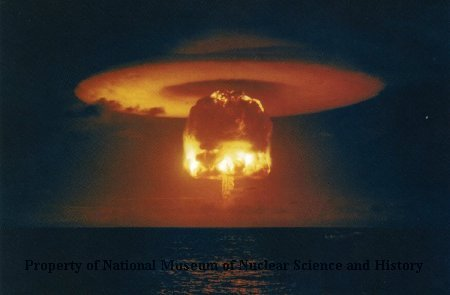
\includegraphics[width=\linewidth]{images/atomicbomb.jpg}%
\\[\jot]\flushleftright\color{mpcolor}\emph{Hydrogen Bomb Test, 1954%
}\\{(\furl{https://nuclearmuseum.pastperfectonline.com/Archive/716477C1-5E7A-485C-8BE1-857919471563}{National Museum of Nuclear Science \amp\ History})}%
}
%
The \furl{https://www.britannica.com/science/nuclear-fission}{atomic bomb} is a dark example of the fact that mass is energy. In phenomena of nuclear fission, we notice a decrease in the weight, measured at rest, of nuclear material before and after the phenomenon of fission. But we also observe that a great amount of (kinetic) energy is released. This amount is exactly equal to the apparently missing weight.

\paragraph{Electric heater.}

As a final example consider a \qty{1000}{W} electric heater, which is radiating \qty{1000}{J} in one second. The heater is also losing around \qty{0.00000000000001}{kg} of mass every second owing to this heat radiation -- although it's also acquiring the same amount of mass as electromagnetic energy.


\subsection{The practical use of the words \enquote*{mass} and \enquote*{energy}}
\label{sec:dist_mass_energy}

From the examples above it becomes clear that energy and mass are two names for the same thing.
The equivalence between energy and mass is given by the famous formula $E=m c^{2}$, where $c$ is the speed of light, \eqn~\eqref{eq:c}. In their respective units this gives
\begin{equation*}
  \begin{gathered}
    \qty{1}{kg} = \qty{89875517873681764}{J}\quad\text{(exactly)}
    \\
    \qty{1}{J} \approx \qty{0.0000000000000000111265}{kg}
  \end{gathered}
\end{equation*}
%
\marginpar{\vspace{-5\baselineskip}\footnotesize\color{mpcolor}\enquote{\emph{%
we are led to the more general conclusion: The mass of a body is a measure of its energy content; if the energy changes by $L$, the mass changes in the same sense by $L/9\!\cdot\!10^{20}$, if the energy is measured in ergs and the mass in grams.
%\par Perhaps it will prove possible to test this theory using bodies whose energy content is variable to a high degree (e.g., salts of radium).
}}\sourceatright{\cites{einstein1905d}}%
}
%
To grasp these numbers, consider that the mass of the rubber band in the example above, \qty{0.5}{g}, is comparable to the energy released by the \furl{https://www.britannica.com/story/atomic-bombing-of-hiroshima}{atomic bomb over Hiroshima}.

But it also becomes clear that in our daily experience we deal with \energym\ in two different ways:

On the one hand, we deal with huge (atom-bomb-like) amounts of \energym\ packed in very small volumes: the huge amounts of \energym\ that go together with objects and stuff like pens, keys, bicycles, cars, houses, water, and so on. We move, push, pull these huge \energym\ amounts from one place to another, and even put them in our pockets. We ourselves are huge bundles of \energym\ moving around. These  amounts of \energym\ change a little, all the time, as in the examples with the rubber band above. But these changes are so small as to be often undetectable with ordinary weight scales, and negligible for practical purposes. We use the word \enquote*{mass} for any such huge amount of \energym, and measure it with a unit -- \unit{kg} -- that doesn't lead to ridiculously large numbers. And we also agree to neglect the imprecision and fluctuation in its measurement, say any imprecision \furl{https://www.nist.gov/si-redefinition/kilogram-disseminating-new-kilogram}{under \qty{0.00001}{\percent}}.\enskip So we say \enquote{the rubber band has a mass of \qty{0.0005}{kg}}, rather than \enquote{the rubber band has an \energym\ of \qty{45000000000000}{J}}.

% This situation is similar to our measuring the power produced by power plants in megawatts (MW). We can say that another power plant constantly produces \qty{500}{MW}; but with this we don't really mean that it produces \emph{exactly} \qty{500000000.000}{W}: there are fluctuations all the time. And we can say that a power plant produces twice as much power, \qty{1000}{MW}, again with the understanding that the ratio is not \emph{exactly} \num{2.000000000000}.

On the other hand, we also deal with the small energy changes and exchanges in all these objects. These energy exchanges that are very important for our daily life: they keep us warm, keep our cells active, make our laptops work. In dealing with these energy exchanges, we don't care about the huge energy reservoirs they come from. So we agree to measure them with a unit -- \unit{J} -- that doesn't lead to ridiculously small numbers. And we also agree not to be precise about the total amount in the reservoir from which these energy bits come from.

As an analogy, think of when we speak about the amount of people in different countries. We can say that in Norway there are \num{5} millions, and in India \num{1500} millions, so in India there are \num{300} times more people. By this we don't mean that in Norway there are \emph{exactly} \num{5000000} people and that India has \emph{exactly} \num{300} times more people. These numbers are changing slightly all the time, but we don't care about differences of 10 or even \num{10000} people. At the same time, if we have three dear friends or relatives visiting us from abroad, then the amount of \num{3} people is now for us very important -- even if it is a very small amount compared to the total population of a country.

\medskip

The distinction above is of course not clear-cut. In dealing with some physical phenomena, for example with few molecules or with subatomic particles, the fictitious but pragmatic distinction between mass and energy becomes too blurry and not useful anymore. In discussing these phenomena, indeed, one often uses the terms \enquote*{mass} and \enquote*{energy} interchangeably, as well as a common unit for both, such as the \furl{https://home.cern/tags/13-tev}{\emph{electronvolt}}.

\medskip

% From the examples above it is clear that the energy changes that we deal with and use in everyday situations are extremely small changes in mass -- so small that we can't measure them within the precision of ordinary weighing scales. Vice versa, the masses that we ordinarily deal with are huge amounts of energy. If we spoke only of \enquote*{energy} or only of \enquote*{mass} in all situations, and used only one unit, either joules or kilograms, we would have to work with very impractical numbers. \enquote*{Mass} can be considered a convenient term for \enquote*{energy} when huge amounts of it are involved, concentrated in small regions of space, and ordinary small energy changes can be neglected.
In these notes we shall often use the expressions \enquote*{\energym} and \enquote*{\masse} to remind ourselves that these two words denote the same physical thing.

\subsection{Different \enquote*{forms} of \energym}
\label{sec:forms_energy}

We often speak of different \emph{forms} of \energym. The most important forms for us will be \textbf{internal \energym}, \textbf{kinetic \energym}, \textbf{gravitational potential \energym}, \textbf{electromagnetic \energym} to be discussed later.

The differences among these forms of \energym\ arise from the way they are calculated from other quantities, as we shall see later. For example, if in a volume there's an amount of a particular kind of matter, then in that volume there must also be an amount of \energym, given by a formula that involves the amount of matter. And if that matter is moving, then we have to add an extra amount of \energym\ given by another formula which involves the velocity. And if in that volume there's a gravitational field (that is, a particular kind of spacetime curvature), then another extra amount of \energym\ must be added, given by yet another formula involving the gravitational field. Similarly if we know that an electromagnetic field is in that volume.

We also speak of different forms of flux of \energym. The most important for us will be \textbf{heat} and \textbf{mechanical power}. The difference is again in how these fluxes are calculated depending on whether there are also fluxes of matter and of other quantities.

%
\marginpar{\vspace{\baselineskip}\footnotesize\centering\includegraphics[width=\linewidth]{images/molecules_20nmb.png}%
\\[\jot]\flushleftright\color{mpcolor}\furl{https://doi.org/10.4209/aaqr.2019.04.0177}{Hydrocarbon fuel particles}. The small blobs have size of around \qty{2e-8}{m}.%
}%
The distinctions between different forms of \energym\ also depend on the observation scale and the theory used. Take, for instance, the water in a glass resting on table. We can observe and describe that water on a macroscopic scale of centimetres, seeing it as a still, uniform fluid. On this macroscopic scale we say that the water has internal \energym, or that there is internal \energym\ in the glass. But we can also observe and model that same water as a collection of molecules, on a microscopic scale of nanometres (\qty{e-9}{m}). On this microscopic scale, we speak of internal \energym\ \emph{and} kinetic \energym, because the molecules are in constant motion. The \emph{total} amount of \energym\ is the same on the centimetre-scale and on the microscopic scale, but its partition into different \enquote{forms} depends on the scale: only internal on the macroscopic scale, and internal plus kinetic on the microscopic scale.

The same is true of flux of \energym. What we call \enquote*{heat} on one observation scale appears as a flux of \energym\ not associated with the motion of matter. But on a finer scale it is instead called \enquote*{work}, and it appears as an \energym\ flux associated with the microscopic motion of matter. % In phenomena that involve matter and electromagnetic fields, any separation between \enquote*{energy of matter} and \enquote*{energy of electromagnetic field} is often arbitrary.

% \begin{warning}[Amounts of \energym\ are coordinate-dependent]
%   Never change coordinate system in the middle of a calculation of energy change!
%   Although the distinction of energy forms is often useful, it's important to keep in mind that it is not absolute: \emph{it depends on the coordinate system, on the scale of observation, and on the theory used}.
% \end{warning}

% So whenever you hear about a distinction between forms of energy or energy fluxes, pay attentionwhich coordinate system and which observation scale are being used.

% Energy-mass is present wherever there's matter, charge, or magnetic flux, and vice versa. \emph{Its specific relation with these quantities depends on the coordinate system} (\sect\,\ref{sec:coords}) that we choose. It is extremely important to keep in mind this dependence. For instance, in the examples above we said that the unstretched rubber band in motion had a \masse\ of \qty{0.000500000000000002}{kg}; but if we choose a coordinate system in which the band is not moving, its \masse\ would be \qty{0.000500000000000000}{kg}. Owing to this coordinate dependence, and depending on whether matter or magnetic flux is present in a region, we often conveniently partition an amount of energy into different \enquote{forms} like rest energy, internal energy, kinetic energy, gravitational potential energy, electromagnetic energy. This is only a conceptual division.
%
% Also energy flux can be partitioned depending on the coordinate system and on whether there's also a flux of matter. This leads to the important distinction between two forms of energy flux: \textbf{heat} and \textbf{work}.
%
% We shall see later how to define and calculate these different forms of energy and energy flux.


\begin{exercise}
  In an hour, 14 people exit through a door. Taking the average human weight to be \qty{62}{kg} \parencites{walpoleetal2012}, what's the average flux of \emph{\energym} t, in \unit{J/s}, through that door?
\end{exercise}



% *** we shall see later in \sect

% electron: 8.2e-14 J
% 1e4 J intake
% 1 cal = 4 J
% 1 kg = 9e16 J
% U = 50/2*0.1^2 = 0.25 J = 3e-18 kg

%\clearpage
\section{Momentum}
\label{sec:intro_momentum}

\marginpar{\vspace{2\baselineskip}\footnotesize\centering\includegraphics[width=\linewidth]{images/walking.jpg}%
\\\flushleftright\color{mpcolor}A walking person has, with respect to the ground, an amount of horizontal momentum of around \qty{70}{N\,s} (\furl{https://www.flickr.com/photos/33486695@N06/13566555795}{image: Antonio Romei}).%
\par\bigskip\centering\normalsize\includegraphics[width=0.75\linewidth]{images/flashlight.jpg}%
\\\footnotesize\flushleftright\color{mpcolor}A \qty{10}{cm} beam of light from a \qty{60}{W} torch has an amount of momentum around \qty{e-16}{N\,s}.%
}%
\begin{definition}{Momentum: units and notation}
  Momentum, also called \emph{linear momentum} or \emph{translational momentum} to distinguish it from angular momentum, is a \emph{vector} quantity. The amount of momentum can be expressed in several equivalent units; we shall keep in mind especially these three:
  \begin{equation*}
    \begin{gathered}
      \textit{newton second}\\
      \unit{N\cdot s}
    \end{gathered}
\enskip\equiv\enskip
    \begin{gathered}
      \textit{kilogram metre per second}\\
      \unit{kg\cdot m/s}
    \end{gathered}
\enskip\equiv\enskip
    \begin{gathered}
      \textit{joule second per metre}\\
      \unit{J\cdot s/m}
    \end{gathered}
\end{equation*}

\smallskip

Flux of momentum is also called \emph{contact force} or \emph{surface force}. Supply of momentum is also called \emph{body force} or \emph{volume force}. They can be expressed in several equivalent units:
\begin{equation*}
    \begin{gathered}
      \textit{newton}\\
      \unit{N}
    \end{gathered}
\enskip\equiv\enskip
    \begin{gathered}
      \textit{kilogram metre per squared second}\\
      \unit{kg\cdot m/s^{2}}
    \end{gathered}
\enskip\equiv\enskip
    \begin{gathered}
      \textit{joule per metre}\\
      \unit{J/m}
    \end{gathered}
\end{equation*}

Since momentum and momentum flux are vector quantities, they are usually expressed with three numbers, typically their $x$-, $y$-, and $z$-components.

\smallskip

The amount of momentum in a volume is usually denoted $\yP$. The flux of momentum (surface force) is denoted $\yF$; and supply of momentum (volume force), $\yG$.
\end{definition}


Momentum is a subtle quantity, even subtler than \energym. Textbooks that focus on Newtonian mechanics \emph{define} it as the product of the mass and the velocity of a body, usually written \enquote{$\bm{p}=m\bm{v}$}. This relation, however, is only valid in special circumstances, and cannot be used in many everyday technological applications, especially when electromagnetism or high speeds are involved. And that relation is actually only an approximation even in the circumstances where it's used. For example, in a small region where there are matter and electromagnetic fields, momentum is approximately given by $\yP=\ym\yv + \yEE\times\bm{H}/\yc^{2}$, where the quantities $\yEE$ (electric field strength) and $\bm{H}$ (magnetic field strength or free-current potential) are related to the electromagnetic properties of matter. And at high speeds, the momentum of matter is better approximated by
% $\yP = \ym\yv + (\yU + \tfrac12 \ym v^{2} + \ym g z)\yv/\yc^{2}$,
$\yP = (\ym + \yE/\yc^{2})\yv$, where $\ym$ is the rest-\energym\ and $\yE$ is the remaining \energym\ of matter.

% First, it is true that where there's matter in motion there's also momentum; but this momentum is given by \enquote*{mass${}\times{}$velocity} only as an approximation. Second, there can be momentum also where there is no matter; for instance where there is magnetic flux. If you prepare a sealed glass box which is completely empty of matter within (you create a vacuum), there still is momentum within the box if light or electromagnetic waves are present. We shall discuss later some technological uses of this fact.

It is therefore beneficial to separate our idea of momentum from the \enquote{mass-times-velocity} formula, keeping in mind that the latter is just a particular case of momentum. Instead, think of momentum as \emph{something associated with translational motion} of matter and of electromagnetic fields. Translational motion is the kind of motion that leads to a new position in space. For instance, when you walk from one place to a different one, you have performed translational motion (note that translational motion doesn't need to be in a straight line).
% We shall moreover see that there is an important connection between momentum and our intuitive idea of \enquote*{force}.
So if something -- be it matter or a magnetic-flux line -- is changing its position in space, then that something has momentum. Indeed in many languages -- for example Chinese, French, Italian, Japanese, Norwegian, Spanish, Swedish -- the term for momentum is literally \enquote*{quantity of motion}.

% Just as energy can be mentally visualized as a sort of fluid, also momentum can be visualized as a sort fluid; but we must imagine it as a \enquote{fluid of vectors}. Just as with energy, this visualization comes with many warnings though.
% \marginpar{%
% \includegraphics[align=t,width=\linewidth]{images/cubearrow.pdf}
% \\[\jot]\footnotesize\color{mpcolor}The amount of momentum within a volume is represented by a \textcolor{cyan}{(3D) vector}%
% }
%
\marginpar{\vspace{-5\baselineskip}\footnotesize\centering\includegraphics[align=t,width=\linewidth]{images/cube_Ns_coords.jpg}%
\\[\jot]\flushleftright\color{mpcolor}The amount of momentum within a volume at a given instant is represented by a \textcolor{purple}{vector}%
}%
Given a particular volume at a particular instant in time, and given a coordinate system, we can speak of the total amount of momentum within that volume. This amount is represented by a \emph{vector}. You can imagine a continuous collection of vectors filling the volume, possibly with different directions and small magnitudes; the total momentum is the sum of all these vectors. This visualization obviously comes with many warnings, but it can be very useful if we are careful.

\medskip

Production of momentum, and flux of momentum in particular, is what we call \textbf{force}. Whenever we exert a force on an object, for instance when we pull a door or simply hold a bag, we are transferring momentum between us and that object. The force of gravity, or weight, that we feel every day in our bodies, is a continuous production of momentum that happens because of the huge \masse\ of the Earth. The force that presses you against your seat when you sit in an accelerating car or in an aeroplane taking off, is also a production of momentum. The term \enquote*{force} is therefore synonymous with \enquote*{flux of momentum} or \enquote*{production of momentum}.

% There are two kinds of forces: \textbf{contact forces}, also called \emph{surface forces}; and \textbf{body forces}, also called \emph{volume forces}.

% Force is a notion that we understand intuitively and that we can \enquote{feel} with our own bodies. In Newtonian mechanics it's often taken as primitive, and is represented by a vector. But it can also be defined and interpreted as a \emph{flux of momentum}. This point of view can be very useful and even more intuitive in some situations. We shall discuss it more in depth in \chap~\ref{cha:contents_fluxes}

\begin{extra}{Momentum and \energym\ flux are proportional}
  According to Relativity Theory, momentum is always proportional to \energym\ flux, and \energym\ flux is always proportional to momentum. If we represent the magnitude of momentum in a volume $V$ with $P$, and the flux of total \energym\ through an area $A$ with $\yH$, their proportionality can be approximately expressed as
  \begin{equation}
    \label{eq:momentum_heat}
    \frac{\yH}{A} \approx \frac{P}{V}\,\yc^{2} \ .
  \end{equation}
  Compare this formula with $\yE=\ym\,\yc^{2}$. From this point of view, you can think of momentum as \enquote{\energym\ in motion}. % This is consistent with our discussion about \masse: since mass is energy, the Newtonian expression \enquote{$m\bm{v}$} indicates energy in motion, or a flux of energy. 
  % On a sunny day, if you close your eyes and feel the Sun's heat on your face, what you are feeling is also a flow of momentum. And when you kick a football, giving it momentum, you've also set a huge bundle of energy in motion.
\end{extra}

\begin{exercise}
  Assume the relation $P = \ym v$ between the magnitude of momentum $P$, \masse\ $\ym$, and its speed $v$. When you're walking with a speed of \qty{1}{m/s}, how much momentum does your body contain?
\end{exercise}



\section{Angular momentum}
\label{sec:intro_angmomentum}

\marginpar{\vspace{2\baselineskip}\footnotesize\centering\includegraphics[width=\linewidth]{images/spin_dancer.jpg}%
\\\flushleftright\color{mpcolor}A spinning dancer has, with respect to the ground, an amount of angular momentum of around \qty{10}{N\,m\,s} (\furl{https://www.rg-dance.com/richardalstondancecompany/}{image: RG-Dance}).%
}%
\begin{definition}{Angular momentum: units and notation}
  Angular momentum, also called \emph{moment of momentum} or \emph{rotational momentum}, is a \emph{vector} quantity. The amount of angular momentum can be expressed in several equivalent units; we shall keep in mind especially these three:
  \begin{equation*}
    \begin{gathered}
      \textit{newton metre second}\\
      \unit{N\cdot m \cdot s}
    \end{gathered}
\enskip\equiv\enskip
    \begin{gathered}
      \textit{kilogram squared metre per second}\\
      \unit{kg\cdot m^{2}/s}
    \end{gathered}
\enskip\equiv\enskip
    \begin{gathered}
      \textit{joule second}\\
      \unit{J\cdot s}
    \end{gathered}
\end{equation*}

\smallskip

Flux of angular momentum is also called \emph{contact torque}. Supply of momentum is also called \emph{body torque}. They can be expressed in several equivalent units:
\begin{equation*}
    \begin{gathered}
      \textit{newton metre}\\
      \unit{N\cdot m}
    \end{gathered}
\enskip\equiv\enskip
    \begin{gathered}
      \textit{kilogram squared metre per squared second}\\
      \unit{kg\cdot m^{2}/s^{2}}
    \end{gathered}
\enskip\equiv\enskip
    \begin{gathered}
      \textit{joule}\\
      \unit{J}
    \end{gathered}
\end{equation*}

Since angular momentum and its flux are vector quantities, they are usually expressed with three numbers, typically their $x$-, $y$-, and $z$-components.

\smallskip

The amount of angular momentum in a volume is usually denoted $\yL$. The flux of angular momentum (surface torque) is denoted $\yM$; and supply of angular momentum (volume torque), $\yto$.
\end{definition}

Given a particular volume at a particular instant in time, and given a coordinate system, we can speak of the total amount of angular momentum within that volume. This amount is represented by a vector.
% %
% \marginpar{\vspace{-15\baselineskip}\footnotesize\centering\includegraphics[width=\linewidth]{images/cube_Nms_coords.jpg}%
% \\[\jot]\flushleftright\color{mpcolor}The amount of angular momentum within a volume at a given instant is represented by a \textcolor{purple}{vector} (curious about the little circulation symbol around the vector? see \sect\,\ref{sec:twisted_vec})%
% }%


\medskip

Just as momentum is associated with translational motion, angular momentum is \emph{something associated with rotational motion} of matter and of electromagnetic fields. Rotational motion is the kind of motion that leads to a \emph{new orientation} in space, rather than to a new position. For instance, if you turn to your left or to your right while standing in place, you have performed a rotational motion.

You can get a feeling of angular momentum and torque by playing with one of those hand-held gyroscopes that can be used for wrist exercise (side figure). But the physical role of angular momentum is actually in front of us every day: its balance is the chief reason of such important phenomena as the alternation of day and night and the alternation of the seasons.
%
\marginpar{\vspace{-8\baselineskip}\footnotesize\centering\includegraphics[width=0.67\linewidth]{images/wristroller.jpg}%
\\[3\jot]\includegraphics[width=\linewidth]{images/fourseasons.jpg}%
}%

\medskip

Yet, angular momentum is seen as an even subtler quantity than momentum, and usually is less in the spotlight than momentum. This happens for several reasons.

One reason is that the distinction between momentum and angular momentum is not clear-cut, and depends on our choice of coordinates. For instance, what can be considered as a component of momentum in one coordinate system, can also be considered as a component of angular momentum in another coordinate system. This reflects the fact that there isn't a clear-cut distinction between translational and rotational motion; usually they involve each other to some degree. A translational motion can be interpreted as a rotation around a point that is very far away; and a rotation of an extended object can be interpreted as a collection of small translational motions of its parts.

Another, very important reason is that the physical laws that involve angular momentum can be expressed in a different way, as sorts of symmetries between momentum fluxes and between \energym\ flux and momentum. With this alternative approach we don't even need to introduce the quantity \enquote*{angular momentum} at all! This approach is indeed followed for many physical phenomena and applications, for example those that involve fluid motion. But for other phenomena it's much more convenient to speak of angular momentum and to use its balance law.
%
\marginpar{\vspace{-14\baselineskip}\footnotesize\centering\includegraphics[width=0.67\linewidth]{images/polymer.png}%
  \\\includegraphics[width=\linewidth]{images/polymer2.png}%
  \\[\jot]\flushleftright\footnotesize\color{mpcolor}Some liquid polymers (\textbf{top:} Liquid Diethoxymethane Polysulfide) need to be described with a special kind of angular momentum, owing to their molecular structure (\textbf{bottom}).%
}%
% \begin{marginfigure}\footnotesize%
%   \includegraphics[align=b,width=\linewidth]{images/polymer.png}
% \\\includegraphics[align=c,width=\linewidth]{images/polymer2.png} \\[\jot]%
% {\color{green}Some liquid polymers (\textbf{top:} Liquid Diethoxymethane Polysulfide) need to be described with a special kind of angular momentum, owing to their molecular structure (\textbf{bottom}).}
% \end{marginfigure}
In phenomena involving liquid \furl{https://www.britannica.com/science/polymer}{polymers},
% https://www.britannica.com/science/polymer
elementary particles, or electromagnetic radiation, for example, it's convenient to use angular momentum and to let it include an additional part, called \emph{spin} or \emph{intrinsic angular momentum}, which is associated with rotational motion that is invisible to the naked eye or the particular instruments used to measure motion.

\medskip

We shall further discuss these topics in \chap~\ref{cha:bal_ang_momentum}. In any case keep in mind that \emph{there is} a universal law that is \emph{independent} from the one obeyed by momentum. Even if we can in principle omit the notion of angular momentum, we \emph{cannot} avoid the use of this additional universal law.


%\cites{truesdell1963b_r1968} tells some of the story of how this was discovered. % \mynotew{rephrase this}

\begin{exercise}
  Assume the relation $L = \ym v R$ between the angular-momentum magnitude $L$, \masse\ $\ym$, speed $v$, and orbital radius $R$ of a planet. \furl{https://nssdc.gsfc.nasa.gov/planetary/factsheet/earthfact.html}{For the Earth} we have approximately
  \begin{equation*}
    \ym = \qty{6.0e24}{kg} \qquad
    v = \qty{3.0e4}{m/s} \qquad
    R = \qty{1.5e11}{m}
  \end{equation*}
How much is the Earth's angular momentum? (Note that we are neglecting the angular momentum coming from its own rotation.)
\end{exercise}


\section{Energy-mass, momentum, angular momentum are coordinate-dependent}
\label{sec:energy_momentum_angmomentum_coords}


%
\marginpar{\vspace{\baselineskip}\footnotesize\centering\includegraphics[width=\linewidth]{images/cube_J_coords.jpg}%
\\[\jot]\flushleftright\color{mpcolor}\enquote{How much \energym\ is there in this volume at this instant?} This question cannot be answered until we have specified which coordinate system we're using.%
}%
An aspect of \energym, momentum, angular momentum that must always be kept in mind is that \textbf{their amounts depends on the coordinate system we're using}. If someone points at a specific region of space at a particular instant, and asks \enquote{how much \energym\ is there?}, we \emph{cannot} give an answer until a coordinate system is specified. Once the coordinate system has been chosen, then a precise and unambiguous answer can be given. The same is true for the flux of \energym\ through a surface, and for the amounts, fluxes, supplies of momentum and of angular momentum. This coordinate-dependence also means that observers using different coordinates will usually assign different amounts of \energym, momentum, angular momentum to the same regions of spacetime.

This is an important difference between \energym, momentum, angular momentum on one side, and matter, electric charge, magnetic flux on the other side. \emph{For matter, electric charge, magnetic flux, the questions about their contents and fluxes can be answered unambiguously independently of any spatial coordinate system}.

This coordinate-dependence is not a problem: we must in practice always specify our coordinate system anyway, in order to agree on the time and position of physical events. But it can cause problems if we calculate or measure some amount of \energym\ at a given time and place using a coordinate system, and we calculate or measure some amount at another time or place using a \emph{different} coordinate system. Combining these two amounts, or using them in the same physical law, has no meaning whatsoever.

\begin{warning}[{{Amounts of \energym, momentum, angular momentum are coordinate-dependent}}]
  Never change coordinate system in the middle of calculations about \energym, momentum, or angular momentum!
\end{warning}

% Also the distinction among different forms of energy is coordinate-dependent. For instance, in one coordinate system we can say that a given volume contains only internal energy; but in another coordinate system that same volume can be said to contain internal and kinetic energy.


\bigskip

\begin{extra}{{What are \energym, momentum, angular momentum?}}
From the discussions and formulae above, it seems that \energym, momentum, angular momentum are quite closely related to one another. For all three, the amount in a volume or through a surface is undefined unless we specify a coordinate system. And we shall see later that all three satisfy balance laws but not necessarily conservation laws.

  Relativity Theory indeed shows that \energym, momentum, angular momentum are different aspects of one single geometric object, called \emph{energy-momentum tensor}. They are like its \enquote{shadows}, that we can observe by looking at it from different points of view in time and space. This is also why their values get intermixed if we change our system of coordinates. This topic will be discussed in \chap~\ref{cha:energymomentum}.

  General Relativity gives a new meaning to these quantities: they are \emph{particular curvatures of spacetime}. They express how spacetime is curved in different directions. So whenever we measure, say, the \energym\ or the momentum of some object or of some electromagnetic radiation, we are actually measuring how much that object or radiation is curving spacetime in a particular way. % We shall discuss further connections between these three quantities and spacetime in \sect\,\mynotew{}.
\end{extra}
\marginpar{\vspace{-12\baselineskip}\footnotesize\centering\includegraphics[width=\linewidth]{images/curvature1.png}%
\\[\jot]\flushleftright\color{mpcolor}Energy-mas, momentum, angular momentum are measures of particular curvatures of spacetime.%
}%

\section{Entropy}
\label{sec:intro_entropy}

\begin{definition}{Entropy: units and notation}
  Entropy is a \emph{scalar} quantity. The unit for entropy content is the \emph{joule per kelvin} \unit{J/K}; the unit for entropy flux is \emph{joule per kelvin per second} \unit{J/(K\,s)}.

  \smallskip

  The amount of entropy in a volume is usually denoted $\yS$. The flux of entropy through a surface is denoted $\yB$.
\end{definition}

From its SI physical dimension and unit, entropy would seem to be derived from temperature. However, although \textsc{temperature} is taken as primitive quantity by the SI, the \furl{https://doi.org/10.1351/goldbook.K03374}{definition of temperature} actually depends on a fixed value of \furl{https://doi.org/10.1351/goldbook.B00695}{\emph{Boltzmann's constant}}, which has the dimension of \textsc{entropy}.

\medskip

Entropy is probably the most difficult quantity to grasp intuitively. Many seemingly intuitive descriptions given in some textbooks are, unfortunately, unhelpful and even misleading.
One particularly \emph{misleading} description is to say that entropy is a \enquote{measure of disorder}. Besides the fact that \enquote{disorder} is a very vague and subjective notion, it turns out that some physical phenomena, for example involving \furl{https://www.britannica.com/science/liquid-crystal}{liquid crystals}, can be considered more \enquote{disordered}, and yet have \emph{lower} entropy, than others. See also the example in the side figure. We shall discuss more about such phenomena later on.
%
\marginpar{\vspace{-8\baselineskip}\footnotesize\centering%
\includegraphics[width=0.495\linewidth]{images/entropy_low.png}\hfill%\\%
\includegraphics[width=0.495\linewidth]{images/entropy_high.png}
\\[\jot]\flushleftright\footnotesize\color{mpcolor}Two microscopic configurations of a lattice gas. \textbf{Left}: configuration coming from a \emph{low}-entropy state. \textbf{Right}: configuration coming from a \emph{high}-entropy state \parencites{styer2000}.%
}%

In these notes we shall rely on the idea that \emph{entropy expresses a limit on the flux of a particular kind of \energym}. Said in simpler but more imprecise words, entropy is a bound on how fast we can heat something up. We shall develop this idea further later.

One reason why entropy is difficult to grasp intuitively is that it has very different physical and mathematical aspects depending on the spatial scales and physical theory that we use to describe physical phenomena.

In many \enquote{continuum} phenomena, that is, phenomena where the molecular constitution of matter is not visible or not taken into account, entropy is treated as a \enquote{stuff-like} quantity similar to \energym\ or electric charge. But there are difficulties also in this case. For some phenomena, for example involving non-elastic materials such as a simple paper clip, it is possible to introduce several entropies having different values -- and not just because of a change in measuring scale -- all of which can serve their purpose perfectly fine.

In molecular phenomena involving statistical mechanics, on the other hand, entropy is no longer a physical notion, but a \emph{probabilitistic} and \emph{statistical} one, related to guesses and inferences that we make about the physical phenomenon. Yet from many points of view it has roles similar to those of the entropy used in continuum phenomena.

We shall see later that the physical laws for entropy have also a different status with respect to the laws for the other six main quantities: they are, so to speak, \enquote{laws about laws}.


\section{Auxiliary quantities}
\label{sec:aux_quantities}

Besides the seven principal quantities, other auxiliary quantities appear in some physical theories. Important examples are \emph{temperature}, \emph{metric}, \emph{strain}, \emph{magnetization}. Some auxiliary quantities are not extensive; for instance we cannot ask \enquote{what's the total amount of temperature in this region?}.


The dimensions, units, and scalar or vector character of all quantities mentioned so far are summarized in table~\ref{tab:units} on page~\pageref{tab:units}.

\subsection{Temperature}
\label{sec:temperature}

We have an intuitive understanding of the notion of \emph{hotness} and \emph{coldness}. Temperature quantifies these notions. The physical bases and measurement procedures for this quantification are far from trivial, but we shall take them for granted in the present notes.

For some physical phenomena, especially those involving gases, we know that temperature is related to the invisible motion of microscopic parts of matter, such as molecules. But there are also physical phenomena for which our microscopic understanding of temperature is more complex, and in some cases  still unclear.

\medskip

Temperature is a \emph{scalar} quantity. There are several definitions and scales of measurement for temperature. Of special importance is \furl{https://www.iso.org/obp/ui/\#iso:std:iso:80000:-5:ed-2:v1:en:tab:1}{\textbf{thermodynamic temperature}}, also called \emph{absolute temperature}, which is measured in \emph{kelvins} (\unit{K}). Thermodynamic temperature has the special property of being always positive in most physical phenomena (there are exceptions, especially in some phenomena where \furl{https://www.britannica.com/science/statistical-mechanics}{statistical mechanics} becomes relevant).

In these notes we shall use thermodynamic temperature, denoting it $\yT$. Its relation with Celsius temperature $\yTce$, which is measured in \emph{degrees Celsius} \unit{\degreeCelsius}, is given by
\begin{equation}
  \label{eq:kelvin_celsius}
  \yTce = \yT - \qty{273.15}{K}
\end{equation}
that is, a redefinition of the \enquote{zero} value; for instance\enskip$\qty{25.00}{\degreeCelsius} = \qty{298.15}{K}$\,.\enskip Note that temperature \emph{differences} are the same for the two temperature scales: $\incr\yTce = \incr\yT$, because the constant zero-value cancels out.

\medskip

Temperature is useful because it enters in many physical laws that involve \energym, but it's easier to measure than \energym.
Temperature generally depends on the time and place, so it can be a function of the coordinates: $\yT(t, x,y,z)$.


\begin{extra}{{What is temperature?}}
\emph{Inventing Temperature} by H.~Chang \parencites*{chang2004} gives a brilliant account of the history of invention of temperature, as well as an interesting portrait of how scientific concepts are born and develop.

\smallskip

\emph{Is There a Temperature?} by T.\,S.~Bir{\'o} \parencites*{biro2011} discusses fascinating physical phenomena for which our microscopic understanding of temperature is still incomplete.%
\end{extra}



\section{Metric}
\label{sec:metric}

A very important quantity is a fundamental building block of all our physical theories: the \textbf{metric}. It is quite different from the seven fundamental quantities, from a physical and also from a geometrical point of view.

The metric characterizes our measurements of space and time. It's the object that allows us to calculate how much \emph{physical} time has elapsed, the \emph{physical} distance between two objects, the volume (say, in cubic metres) of a three-dimensional region of space, and the area (say, in square metres) of a surface. In General Relativity the metric allows us to calculate the curvature of spacetime.

The metric itself, in the technical sense of the so-called \enquote{metric tensor}, is \emph{not} an extensive quantity. We can't ask \enquote{what's the total amount of metric in this region?}; that's a meaningless question. There are, however, other quantities which can be derived from the metric and which are extensive. Important examples are the so-called \enquote{volume density} and \enquote{area density}, which are the ones that allow us to calculate extended volumes and areas.

In the Newtonian approximation, that is, for speeds smaller than the speed of light and low \energym\ densities (hence weak gravitational fields and small spacetime curvature), the metric is just a static, uniform object, the same everywhere in spacetime; and spacetime is \emph{flat}, that is, it has no curvature. This is why we can speak of an \enquote*{absolute time} and \enquote*{absolute distances} in this approximation. In these notes we shall for the most part use this Newtonian approximation.

In General Relativity the metric is a dynamic object instead: it can change with coordinate time, and can vary from one point in space to another. These changes are determined by the seven main quantities, and the metric, in turn, determines changes in the seven quantities.

\begin{table}
  \centering
  \begin{tabular}{lll}
    \hline\\
    \textbf{Quantity}&\textbf{SI Dimension}&\textbf{Unit}
    \\[2\jot]
    Time&\textsc{time}&\emph{second}\;\unit{s}
    \\[\jot]
    Length&\textsc{length}&\emph{metre}\;\unit{m}
    \\[2\jot]
    Matter&\textsc{amount of substance}&\emph{mole}\;\unit{mol}
    \\[\jot]
    Electric charge&$\textsc{current}\cdot\textsc{time}$&\emph{coulomb}\;\unit{C}
    \\[\jot]
    Magnetic flux&$\textsc{mass}\cdot\textsc{length}^{2}/(\textsc{current}\cdot\textsc{time}^{2})$
    &\emph{weber}\;\unit{Wb}
    \\[2\jot]
    Energy-mass&\parbox[t]{10em}{$\textsc{mass}\cdot\textsc{length}^{2}/\textsc{time}^{2}$,\\[0\jot] \textsc{mass}}&\parbox[t]{5em}{\emph{joule}\;\unit{J},\\[0\jot] \emph{kilogram}\;\unit{kg}}
    \\[7\jot]
    \textbf{Momentum}
    &$\textsc{mass}\cdot\textsc{length}/\textsc{time}$
    % &\parbox[t]{10em}{$\textsc{force}\cdot\textsc{time}$,
    %   \\[0\jot]$\textsc{mass}\cdot\textsc{length}/\textsc{time}$,
    %   \\[0\jot]$\textsc{energy}\cdot\textsc{time}/\textsc{length}$}
    &\parbox[t]{5em}{\unit{N\cdot s},
      \\[0\jot]\unit{kg\cdot m/s},
      \\[0\jot] \unit{J\cdot s/m}}
    \\[12\jot]
    \textbf{Angular momentum}
    &$\textsc{mass}\cdot\textsc{length}^{2}/\textsc{time}$
    % &\parbox[t]{10em}{$\textsc{force}\cdot\textsc{length}\cdot\textsc{time}$,
    %   \\[0\jot]$\textsc{mass}\cdot\textsc{length}^{2}/\textsc{time}$,
    %   \\[0\jot]$\textsc{energy}\cdot\textsc{time}$}
    &\parbox[t]{5em}{\unit{N\cdot m\cdot s},
      \\[0\jot]\unit{kg\cdot m^2/s},
      \\[0\jot] \unit{J\cdot s}}
    \\[12\jot]
    Entropy&$\textsc{mass}\cdot\textsc{length}^{2}/(\textsc{time}^{2}\cdot\textsc{temperature})$&\unit{J/K}
    \\[2\jot]
    Temperature&\textsc{temperature}&\emph{kelvin}\;\unit{K}
    \\[2\jot]
    \hline
  \end{tabular}
  \caption{SI dimensions and units of the main physical quantities used in these notes. Their fluxes have the dimensions divided by time, and therefore units divided by seconds. Quantities in \textbf{boldface} are vectors, the others are scalars.}\label{tab:units}
\end{table}
% \begin{table}[tb]
%   \centering
%   \begin{tabular}{lll}
%     \hline\\
%     \textbf{Quantity}&\textbf{Geometric character}&\textbf{Unit}
%     \\[2\jot]
%     Time&\textsc{scalar}&\emph{second}\;\unit{s}
%     \\[\jot]
%     Length&\textsc{scalar}&\emph{metre}\;\unit{m}
%     \\[\jot]
%     Temperature&\textsc{scalar}&\emph{kelvin}\;\unit{K}
%     \\[2\jot]\color{green}
%     Matter&\color{green}\textsc{scalar}&\color{green}\emph{mole}\;\unit{mol}
%     \\[\jot]\color{purple}
%     Electric charge&\color{purple}\textsc{scalar}&\color{purple}\emph{coulomb}\;\unit{C}
%     \\[\jot]\color{red}
%     \textbf{Magnetic flux}&\color{red}\textsc{vector}&\color{red}\emph{weber}\;\unit{Wb}
%     \\[\jot]\color{blue}
%     Energy&\color{blue}\textsc{scalar}&\color{blue}\parbox[t]{5em}{\emph{joule}\;\unit{J},\\[0\jot] \emph{kilogram}\;\unit{kg}}
%     \\[5\jot]\color{cyan}
%     \textbf{Momentum}&\color{cyan}\textsc{vector}&\color{cyan}\parbox[t]{5em}{\unit{kg\cdot m/s},\\[0\jot] \unit{J\cdot s/m}}
%     \\[5\jot]\color{yellow}
%     \textbf{Angular momentum}&\color{yellow}\textsc{vector}&\color{yellow}\parbox[t]{5em}{\unit{kg\cdot m^2/s},\\[0\jot] \unit{J\cdot s}}
%     \\[5\jot]\color{midgrey}
%     Entropy&\color{midgrey}\textsc{scalar}&\color{midgrey}\unit{J/K}
%     \\[2\jot]
%     \hline
%   \end{tabular}
%   \caption{Dimensions and units of the main physical quantities used in these notes. Quantities in \textbf{boldface} are vectors, the others are scalars}\label{tab:units}
% \end{table}

\printpagenotes*
\cleartooddpage
\chapter{Volume contents, fluxes, supplies}
\label{cha:contents_fluxes}

% \marginpar{\vspace{-2\baselineskip}\mynotew{Under modification}}

\epigraph{%
When we regard energy as residing intrinsically in a body, we may measure its intensity by the amount contained in unit of volume. \textelp{T}he only way we have of defining the motion of the fluid is by considering it as a flux \textelp{}. %, and measuring it by the mass of the fluid which flows through unit of area.
  This distinction is still more necessary when we come to heat and electricity. The flux of heat or of electricity cannot be even thought of in any way except as the quantity which flows through a given area in a given time.%
}{J. Clerk Maxwell \cites*{maxwell1869}}

% \epigraph{The other method of investigation, in which we consider what passes through the walls of an element of volume, is applicable to electric current, and is perhaps preferable %in point of form to that which we have given, but as it may be found in any treatise on Hydrodynamics we need not repeat it here.%
% }{J. Clerk Maxwell \cites*{maxwell1873}}

%   \epigraph{For the sake of persons of these different types, scientific truth should be presented in different forms, and should be regarded as equally scientific, whether it appears in the robust form and the vivid colouring of a physical illustration, or in the tenuity and paleness of a symbolical expression.%
% }{J. Clerk Maxwell \cites*{maxwell1870}}

%mynotew{add intro about the general idea, how we apply physical laws}


\section{Content, flux, supply}
\label{sec:contentflux}

The concept of physical quantity allows us to look at the word in ways that can be quantified and expressed with numbers and mathematics. This is how we can formulate \autoref{sec:phys_laws0}{physical laws}. In the previous chapter we made our acquaintance with seven physical quantities. They were chosen as our building blocks because their quantification is easy to grasp intuitively and to visualize. In the present chapter we study this quantification more rigorously, and start developing the necessary mathematics.

\medskip

For each of the seven primitive quantities, except magnetic flux, we can measure three kinds of amount: \textbf{volume content}, \textbf{flux}, and \textbf{supply}:

%
\marginpar{\vspace{\baselineskip}\footnotesize\centering\includegraphics[height=11em]{images/howmuch_volume_notime.jpg}%
}%
\begin{definition}{Volume content}
  \textbf{Volume content} or \textbf{volume integral} is the amount of quantity contained within a three-dimensional region, at a specific time instant.

  \smallskip

  The volume content of a quantity does \emph{not} depend on how the volume is moving. The volume content has the same physical dimension as the quantity.
\end{definition}

%
\marginpar{\vspace{\baselineskip}\footnotesize\centering\includegraphics[height=11em]{images/howmuch_surface_notime.jpg}%
}%
\begin{definition}{Flux}
  \textbf{Flux} is the amount of quantity flowing through a two-dimensional surface in a given direction, \emph{per time}, at a particular time instant.

  \smallskip

  The flux of a quantity through a surface depends on how that surface is moving and deforming. The flux has the physical dimension of that quantity divided by time.
\end{definition}


\begin{definition}{Supply}
  \textbf{Supply} or \textbf{source} is the amount of quantity being produced or destroyed within a three-dimensional region \emph{per time}, at a particular time instant.

  \smallskip

  The supply of a quantity in a region depends on how that region is moving and deforming. The supply has the physical dimension of that quantity divided by time.
\end{definition}

For the magnetic flux we shall introduce analogous kinds of amount, but in one less dimension.

The volume content, flux, and supply of the four scalar quantities -- matter, electric charge, \energym, entropy -- are also \emph{scalars}; that is, each is expressed by one number and a unit.
The volume content, flux, and supply of the two vector quantities -- momentum and angular momentum -- are also \emph{vectors}; that is, each is usually expressed by three numbers and units.

\section{Symbols, notation, and extensivity}
\label{sec:symbols_quantities}

\begin{table}
  \centering
  \begin{tabular*}{\linewidth}{@{\extracolsep{\fill}}lclll}
    \hline\\[-1ex]
    \textit{Quantity}&& \textit{Vol. content\enskip[unit]} & \textit{Flux\enskip[unit]} & \textit{Supply}
    \\[4ex]
    matter&& $\yN$\enskip[\unit{mol}] & $\yJ$\enskip[\unit{mol/s}]
    & $\ya$
    \\[3ex]
    electric charge&&$\yC$\enskip[\unit{C}] &$\yI$\enskip[\unit{C/s} \textcolor{grey}{\footnotesize or} \unit{A}] &
    \\[3ex]
    \energym&&
    \parbox[c]{5em}{$\yE$\enskip[\unit{J}]\\$\ym$\enskip[\unit{kg}]}
    & $\yH$\enskip\parbox[c]{5em}{[\unit{J/s}\;\textcolor{grey}{\footnotesize or}\;\unit{W}]\\{}[\unit{kg/s}]}
    & $\yR$
    \\[4ex]
    \textbf{momentum}&& $\yP$\enskip[\unit{N\,s}] & $\yF$\enskip[\unit{N}]  & $\yG$
    \\[3ex]
    \parbox[c]{5em}{\textbf{angular\\momentum}}&& $\yL$\enskip[\unit{N\,m\,s}] & $\yM$\enskip[\unit{N\,m}] & $\yto$
    \\[3ex]
    entropy&& $\yS$\enskip[\unit{J/K}] & $\yB$\enskip[\unit{J/(K\,s)}]
    \\[2ex]
    \hline
  \end{tabular*}
  \caption{Symbols and units for volume content, flux, supply of six main quantities. Vector quantities are in \textbf{boldface}. Supplies have the same units as fluxes.}
  \label{tab:symbols_volint_fluxes}

  \vspace{10em}

  \begin{tabular*}{\linewidth}{@{\extracolsep{\fill}}lclll}
    \hline\\[-1ex]
    \textit{Quantity}&& \textit{Flux\enskip[unit]} & \textit{Circuitation\enskip[unit]} & %\textit{Flux supply}
    \\[4ex]
    magnetic flux&&$\yBf$\enskip[\unit{Wb}] &$-\yEv$\enskip[\unit{Wb/s} \textcolor{grey}{\footnotesize or} \unit{V}] &
    \\[2ex]
    \hline
  \end{tabular*}
  \caption{Symbols and units for flux and circuitation of magnetic flux.}
  \label{tab:symbols_flux_circuit}
\end{table}


The three kinds of amount, for each quantity, are denoted by special symbols. Table~\ref{tab:symbols_volint_fluxes} on page~\pageref{tab:symbols_volint_fluxes} summarizes the symbols, units, and scalar or vector character for the volume content, flux, supply of the seven quantities, as used in these notes. Let's see some examples.

\medskip

%
\marginpar{\vspace{0\baselineskip}\footnotesize\centering\includegraphics[height=8\baselineskip]{images/bottle_water.jpg}%
}%
Consider a bottle on a table. You measure the amount of water molecules in it at a given time, and find that it's \qty{51.3}{mol}. We can express this as follows:
\begin{equation*}
  \yN_{\mathrm{H_2O}} = \qty{51.3}{mol} \ .
\end{equation*}
The symbol \enquote*{$\yN$} is used for the volume content of \emph{matter}. The kind of matter in this case is water, so we append its chemical formula $\mathrm{H_2O}$ as a subscript; but we could also have used the word \enquote*{water} or the letter \enquote*{w}. We could also append the word \enquote*{bottle} to indicate that we're speaking about the volume content of the bottle.

\medskip

%
\marginpar{\vspace{\baselineskip}\footnotesize\centering\includegraphics[height=8\baselineskip]{images/two_batteries.jpg}%
}%
As a second example, consider two ordinary batteries inside some device; one is on the left, the other on the right in the battery compartment. You measure the amount of chemical \energym\ in each battery at a given time, and find \qty{9873}{J} for the battery on the left, and \qty{4221}{J} for the one on the right. We can express this as follows:
\begin{equation*}
  \yE_{\text{L}} = \qty{9873}{J} \ ,
  \qquad
  \yE_{\text{R}} = \qty{4221}{J} \ .
\end{equation*}
The symbol \enquote*{$\yE$} is used for the volume content of \emph{\energym}. In this case we're speaking about chemical \energym, and we assume this is clear from the context, so we don't indicate this in the symbols. But we must distinguish the volume contents of the two batteries, so we use the subscripts \enquote*{L} and \enquote*{R}; but we could have used \enquote*{l} and \enquote*{r}, or \enquote*{left} and \enquote*{right}.

\medskip

%
\marginpar{\vspace{\baselineskip}\footnotesize\centering\includegraphics[width=\linewidth]{images/static_comb.jpg}%
}%
As a third example, consider a comb that has acquired electricity, say from rubbing with hair. You measure the net volume content of electric charge in the comb when your stopwatch shows \qty{5}{s}, and find \qty{-0.0000004}{C} (note that the charge is more concentrated at the boundary of the volume). Then you measure it again 10 seconds later and find that there is no net charge. We can express this as follows:
\begin{equation*}
  \begin{aligned}
    \yti &= \qty{5}{s} &\quad \yC(\yti) &= \qty{-0.0000004}{C} \ ,
    \\
    \ytf &= \qty{15}{s} & \yC(\ytf) &= \qty{0.0000000}{C} \ .    % \yti &= \qty{5}{s} &\ytf &= \qty{15}{s}
    % \\
    % \yC(\yti) &= \qty{-0.0000004}{C}
    % \qquad&\yC(\ytf) &= \qty{0}{C}
  \end{aligned}
\end{equation*}
The symbol \enquote*{$\yC$} is used for the volume content of \emph{electric charge}. We assume that it's clear from the context that we're speaking about the charge of the comb, so we don't indicate this in the symbols. The volume content $\yC$ of the charge is changing with time, that is, it is a \emph{function} of time. Thus we indicate its value at different times by explicitly writing its argument in round brackets.

\medskip

The examples above show that it depends on the context what kinds of subscript or additional signs that we use together with the symbols for volume content, flux, supply. We have some freedom in which additional signs to use; what's important is to make the message unambiguous.

Volume content, flux, and supply always refer to some particular time, so strictly speaking they are functions of time and would need a time argument like \enquote*{$(t)$}. But in situations where we are considering one particular time only, or where the quantities are constant in time, we can for brevity omit the time argument.


\subsection{Extensivity or additivity}
\label{sec:extens_sum}

The first kind of mathematical operation that we can do with our seven quantities is related to the other important property common to all of them, \autoref{def:extensivity}{\emph{extensivity} or \emph{additivity}}:
\begin{itemize}
\item The content in a volume consisting of non-overlapping volumes is equal to the \emph{sum} of the contents in the individual volumes.
\item The flux through a surface consisting of non-overlapping surfaces is equal to the \emph{sum} of the fluxes through the individual surfaces.
\item The supply in a volume consisting of non-overlapping volumes is equal to the \emph{sum} of the supplies in the individual volumes.
\end{itemize}
When we speak of sum, we mean an ordinary sum for scalar quantities, and a \emph{vector} sum for vector quantities.

As an example, let's consider again the two batteries. If we take them together, we're considering a new volume, consisting of the volumes of the two batteries. We can denote the content of \energym\ in this volume with\enskip$\yE_{\text{tot}}$\enskip to distinguish it from the contents of the left battery $\yE_{\text{L}}$ and of the right battery $\yE_{\text{R}}$. The content in the combined volume is given by
\begin{equation*}
  \begin{split}
    \yE_{\text{tot}} &= \yE_{\text{L}} + \yE_{\text{R}}
    \\ &= \qty{9873}{J} + \qty{4221}{J}
    = \qty{14094}{J}
  \end{split}
\end{equation*}
and this equation expresses the principle of extensivity.

\section{Control volumes and control surfaces}
\label{sec_controlvolumes_surfaces}

For each of six main quantities we can therefore say how much of that quantity is in a given volume, how much is flowing through a given surface per time, and how much is being created in a given volume per time. But how should we choose such volumes and surfaces? Are we constrained in their choice? Do they need to have particular shapes or sizes or positions? Do they need to follow the contours of particular physical objects?

These volumes and surfaces will play an important role in formulating our main physical laws; so one might think that they must be chosen in very special ways. But that isn't the case!

What's surprising and extremely useful is that \textbf{the choice of volume} for a volume content or supply, \textbf{and the choice of surface} for a flux, \textbf{are completely arbitrary}. Moreover, \textbf{these volumes and surfaces can be completely imaginary}.

Since they are under our control, and since they allow us to keep under control how the amounts of our main quantities change, we call them \emph{control volumes} and \emph{control surfaces}:

\begin{definition}{Control volume}
  A \textbf{control volume} is an arbitrary three-dimensional region of space. This region can have any position, shape, and size, and these can change smoothly in time.

  \smallskip

  A control volume can also consist of several disconnected three-dimensional regions, and it can be completely imaginary.
\end{definition}

\begin{definition}{Control surface}
  A \textbf{control surface} is an arbitrary two-dimensional surface. This surface can have any position, shape, and size, and these can change smoothly in time.

  \smallskip

  A control surface can also consist of several disconnected surfaces, and it can be completely imaginary.
\end{definition}

As explicitly stated in the definitions above, control volumes and control surfaces don't need to be static: they can move and deform.

\medskip

The fact that we can choose control volumes and control surfaces arbitrarily gives us a lot of power in solving physics problems and in simulating and predicting the behaviour of physical phenomena. Control volumes and surfaces are typically chosen so as to simplify the equations that describe the physical situation and to focus on details of interest.

Up to now our discussion has been somewhat abstract. This abstractness reflects the amazing flexibility of the notions of control volumes and control surfaces. We now explore some more concrete examples.



\subsection{Examples}
\label{sec:control_volumes_examples}

Let's start with an informal example of control volume and control surface.

Consider a classroom with some people within. In your imagination you can divide the classroom into two halves, say the front half and the rear half. You effect this division by imagining a two-dimensional, immaterial surface, going from the floor to the ceiling, and from one side wall to the opposite one. The exact position and shape of this imaginary surface are up to you, as long as the surface has a clear crossing direction.
%
\marginpar{\vspace{-2\baselineskip}\footnotesize\centering\includegraphics[width=\linewidth]{images/room_CV.jpg}%
\\[\jot]\flushleftright\color{mpcolor}A classroom with an imaginary, slightly skew surface (in \textcolor{purple}{red}) dividing the front and rear half of the room. (Room design: \furl{https://www.turbosquid.com/3d-models/classroom-1726208}{Raihanali}.)%
}%
% (Room design: \furl{https://sketchfab.com/3d-models/classroom-7f981d3e0b6445108d684abf3f2fd4ab}{Janis Zeps})
% 
% Raihanali

You can then simply measure how many people are in the rear half at a particular time instant, say time 14:43:27 of a specific date. This measurement could be done for instance by taking a photograph at exactly that instant, and then counting the people in the rear half on the photograph.

What you just did was to choose a \emph{control volume} at a given time, and to measure its \enquote{volume content} of people. Note how the control volume in this case was defined partly by real objects (half of the ceiling and floor, half of the side walls, the rear wall) and partly by an imaginary object (your imagined surface dividing the classroom).

\medskip

You can also focus on your imaginary surface only, rather than the room, and with the help of a video camera you can keep track of how many people cross the imaginary surface between times 14:43:27 and 14:43:30. You could for instance observe that in those three seconds 10 people cross the imaginary surface from the rear half to the front half of the room, and 4 people cross it from the front rear. So a net number of 6 people cross from the rear to the front half in three seconds, or 2 people/second on average.

What you just did was to consider a \emph{control surface}, and to measure the \enquote{flux} of people through it. In this case the control surface was defined by an imaginary object (your imagined surface). But you could also consider a different, larger control surface, consisting for instance of the imaginary surface and one side wall. This control surface would be defined partly by a real object (the side wall) and partly by an imaginary object (your imagined surface).

% There can be obvious complications. What if a person is entering the room from the rear door exactly at 14:43:27, and so is partly within the room, partly outside? In this case we must count \enquote{fractions of a person} as being in the control volume; so there could be \num{5.3} people in the control volume at that instant.

\medskip

%
\marginpar{\vspace{-4\baselineskip}\footnotesize\centering\includegraphics[width=\linewidth]{images/kettle_CV.jpg}%
  \\[\jot]\flushleftright\color{mpcolor}Simplified section of a kettle, with a control volume (in \textcolor{purple}{red}) delimited by a closed control surface (\textcolor{purple}{dashed red line}).%
}%
In the previous example the control volume and control surfaces had very simple shapes. We can choose more complex shapes if needed. Take for instance a kettle, and suppose we want to keep track of how much water, steam, air, and maybe \energym\ go into or out of it. The interior of the kettle is our control volume. It is delimited by the interior surface of the metal that makes up the kettle, and also by an imaginary surface at the end of the spout. Note that as we move the kettle around, so do these control volume and control surface. If we make a dent on the kettle with a hammer, then the control volume and control surface will follow that dent.

In a similar way we can consider as control volumes more complicated objects and spaces -- like a car, a rocket, a bacterium, a planet, the chamber in a piston -- with appropriate control surfaces that \enquote{wrap} them. Keep in mind that these control volumes and surfaces bend and move as needed. The locomotive system illustrated on the side can be considered as a control volume, with a complex movable control surface that perfectly wraps every element of it.
%
\marginpar{\vspace{-5\baselineskip}\footnotesize\centering%\includegraphics[width=0.75\linewidth]{images/piston_CV2.jpg}\\%
\includegraphics[width=\linewidth]{images/locomotive.jpg}%
\\[\jot]\flushleftright\footnotesize\color{mpcolor}From \furl{http://www.009.cd2.com}{009 Lynton and Barnstaple Railway County Gate}%
}%

\section{Choices of control volumes and surfaces}
\label{sec:choice_control_volumes}

%
\marginpar{\vspace{\baselineskip}\footnotesize\centering\includegraphics[width=\linewidth]{images/wing_grid.png}%
  \\[\jot]\flushleftright\color{mpcolor}Section view of grid of control volumes and surfaces for studying the flow of air around an aeroplane wing (from \cites{schieffer2013}). The extended white areas are sections of the wing and of its \furl{https://www.grc.nasa.gov/WWW/k-12/VirtualAero/BottleRocket/airplane/flap.html}{slat and flap}.%
% \\[\jot]\includegraphics[width=0.5\linewidth]{images/slat_wing_flap2.jpg}%
}%
The full freedom we have in choosing control volumes and surfaces is extremely powerful for physics and engineering applications. Let's discuss two particular kinds of choice that are often made in two broad types of physical situations, and that we shall also often use in these notes.

\medskip

First choice. When we study solid objects, or objects made of solid parts -- like a football, a book, a car, an aeroplane, a rocket, and in some situations a human being or a planet -- then we use the object itself as a control volume. The control surface tightly \enquote{wraps} the object.

Because of this particular choice, we often say, for instance, \enquote*{the momentum of the tennis ball}, but what it's meant is \enquote*{the momentum in the volume that encloses the tennis ball}.

There are two main reasons for this choice. First, this choice makes one particular physical law, the \autoref{cha:cons_matter}{balance of matter}, automatically satisfied. So we don't need to consider it when describing the physical phenomenon of interest. Second, the movement and deformation of control volumes and surfaces so chosen are not too complicated to represent mathematically; because the object is solid, so its kinds of movement are limited.

\medskip

Second choice. When we study something flowing or moving in a more fluid way -- like a body of water, the atmosphere, fuel or gas in a cylinder, plasma, or an electromagnetic field -- then we divide the space of interest into small, \emph{static} control volumes and surfaces. We essentially construct a \emph{mesh}.

With this choice we do have to explicitly consider the physical law for the balance of matter, making the equations a little more complicated. But at the same time the mathematical representation of these control volumes and surfaces is extremely simple, because they're static.

\medskip

%
\marginpar{\vspace{0\baselineskip}\footnotesize\centering\includegraphics[width=\linewidth]{images/liquidvolume.png}%
  \\[\jot]\flushleftright\color{mpcolor}Clever hybrid choices of control volumes and surfaces allow us to simulate complex motions of fluid surfaces. \furl{http://www.youtube.com/watch?v=M5xnAdVPbgQ}{See also animation} (\cites{wojtanetal2009}).%
}%
There are also hybrid choices between the two special choices above, with some control volumes and surfaces that are static, and others that move and deform in a more fluid way. These hybrid choices are used for instance in simulations of fluids where the behaviour of their surface -- waves, detaching drops, and similar -- are important.


\section{Volume content}
\label{sec:intuition_volume}

\subsection{Scalar quantities}

A volume content (or volume integral) for a scalar quantity, for example \energym, can be represented like this:
\begin{center}
  \includegraphics[align=t,height=7em]{images/volumeintegral_8J.pdf}
\end{center}
we have eliminated one spatial dimension for simplicity, considering the analogous two-dimensional idea. The volume is in \textcolor{midgrey}{light grey}, delimited by a closed \textcolor{darkgrey}{darker grey} boundary, and we're indicating that the volume content, that is, the amount of \energym\ within, is \textcolor{blue}{\qty{8}{J}}.

As a visualization device, this representation can be useful. But let's straighten out some of its aspects:
\begin{itemize}[para]
\item Recall that this is a snapshot at a given time instant. So there are \qty{8}{J} of \energym\ in the volume at that instant, but we don't know the situation earlier or later: there could be a different amount of \energym, the region might be at a different position and have a different shape, or it might not even exist.

\item Recall that some scalar quantities, like electric charge and in some situations matter (antimatter), can have negative amounts.
\marginpar{\centering%
\includegraphics[align=c,width=0.5\linewidth]{images/volumeintegral_6C.pdf}
\\[\jot]\flushleftright\footnotesize\color{mpcolor}A region with a negative amount of charge%
}

\item We must not surmise that the amount of quantity is uniformly distributed within the volume. In fact there could be negative amounts of it in some subvolumes and positive in others. In particular,  even if there is a zero amount of quantity in a volume, some subvolumes could have non-zero amounts: some positive and some negative, so that the total is zero.
  % \begin{warning}
  %  Even if there is a zero amount of quantity in a volume, some subvolumes could have non-zero amounts: some positive and some negative, so that the total is zero.
  % \end{warning}
\end{itemize}

\bigskip

\begin{exercise}
  The volume content of matter in a particular volume is equal to \qty{36}{mol}. Can we conclude that the volume doesn't contain antimatter?
\end{exercise}


\subsection{Vector quantities}\label{sec:volintegral_vector}

A volume content for a vector quantity, for example momentum, can be represented as follows (we still simplify our visualization to two dimensions):
\begin{center}
  \includegraphics[height=7em]{images/volumeintegral_8Ns.pdf}
\end{center}
% \marginpar{\footnotesize
%   \begin{warning}%[Vector magnitudes are positive]
%     Remember that the \emph{magnitude} of a vector is always positive, and that\quad $\mathord{\mathcolor{purple}{\nwarrow}} = -1\cdot\mathord{\mathcolor{blue}{\searrow}}$
%   \end{warning}
% }
Momentum is a vector quantity, so the total amount in the volume above is a vector: the figure shows the direction and orientation of this vector, and the magnitude of \textcolor{blue}{\qty{8}{N\,s}}
is explicitly reported.
\begin{warning}[Vector magnitudes and opposite vectors]
  Remember that the \emph{magnitude} of a vector is always positive, and that\quad $\mathord{\mathcolor{purple}{\nwarrow}} = -1\cdot\mathord{\mathcolor{blue}{\searrow}}$
\end{warning}

The visual representation above is useful, if we keep in mind remarks analogous to the scalar case:
\begin{itemize}
\item This is a time snapshot.
\item\label{item:applicationpoint}The application point of the vector representing the volume content is unimportant: for instance, it doesn't need to be placed at the centre of the volume. The vector refers to the volume as a whole, not to some specific point within.
\item Different subvolumes could have amounts represented by different vectors; only the total vector is represented above.
\end{itemize}
%
\marginpar{\vspace{-6\baselineskip}\footnotesize\centering%
\includegraphics[width=0.5\linewidth]{images/volumeintegral_N_divided.pdf}
\\[\jot]\flushleftright\footnotesize\color{mpcolor}The whole region has zero volume content. The left and right subregions have non-zero and opposite volume contents.%
}%
This last remark is especially important when we discuss momentum and angular momentum. As an example, look at the side figure:
the volume content for the whole region is \emph{zero}, but its left and right subregions have \emph{non-zero and opposite} volume contents.
%
% \begin{figure}[h]\centering
%   \includegraphics[height=7em]{images/volumeintegral_N_divided.pdf}
%   \caption{The whole region has zero volume content. The left and right subregions have non-zero and opposite volume contents.}\label{fig:nonzero_vector_subregions}
% \end{figure}

\bigskip


\begin{exercise}
  Recall \emph{extensivity}, the second property of our seven primitive quantities: the amount in a volume consisting of separate volumes is equal to the total of the separate amounts.

We have a region consisting of two subregions; the amounts of momentum in each subregion are shown below.
  \begin{center}
    \includegraphics[width=0.5\linewidth]{images/exercise_momentumsum.pdf}
  \end{center}
  \begin{enumerate}[exerc]
  \item Write the total momentum in each subregion in component form, $(P_{x}, P_{y})$, according to the coordinate system shown.
  \item Calculate the momentum in the whole region; represent it graphically as vector and write it in component form.
  \end{enumerate}
\end{exercise}

\begin{extra}{Adding vectors in General Relativity}
  We are used to the idea of adding vectors placed at different points in space: we only have to move each vector, keeping it parallel to itself, to a common point; and then add them all at that point with the usual rule.

  This operation \emph{cannot} be done so simply in General Relativity: the notion of parallelism doesn't apply anymore in a simple way, owing to the curvature of spacetime. The addition would lead to different results depending on how we transported the vectors.

  But it is still possible to add the momentum of two different spatial regions, simply because \emph{momentum is defined with respect to a coordinate system}. This coordinate system selects, so to speak, a unique way to transport the momentum vectors to a common point. We are again reminded of the fact that \autoref{sec:energy_momentum_angmomentum_coords}{momentum is a coordinate-dependent quantity}.

  In General Relativity momentum is not really a vector, but just a special triplet of quantities.

  % How can this operation be possible in Newtonian mechanics and in practical applications, then? After all, General Relativity surely applies here! The answer is that the discrepancies of vector transportation are small enough in the neighbourhood of the Earth, as the curvature of spacetime is very small here.
\end{extra}


\section{Flux of scalar quantities}
\label{sec:flux_scalar_direction}

To get an intuitive grip of the notion of flux, consider a %
% \autoref{sec_controlvolumes_surfaces}{flow of people through an open door}.
flow of people through an open door. The door is our control surface. %
We can ask how many people crossed the door during a minute. But one more detail about this flow is important: \emph{in which direction did the people cross the door?} This detail is important because, for example, the door leads to a classroom and we need to keep track of how many seats are free. We therefore need to know whether each person who crossed the door was actually \emph{entering} or \emph{leaving} the classroom.

\marginpar{\vspace{-5\baselineskip}\footnotesize\centering%
\includegraphics[width=0.5\linewidth]{images/person_enter.pdf}
\\\flushleftright\footnotesize\color{mpcolor}According to the crossing direction indicated by the \textcolor{cyan}{blue wiggly arrow}, the person crossing the door counts as\enskip\enquote*{$+1$}.%

\bigskip

\centering%
\includegraphics[width=0.5\linewidth]{images/person_leave.pdf}
\\\flushleftright\footnotesize\color{mpcolor}According to the crossing direction indicated by the \textcolor{cyan}{blue wiggly arrow}, the person crossing the door counts as\enskip\enquote*{$-1$}.%
}%
In order to do this we can proceed as follows:
\begin{enumerate}[label=\arabic*.]
\item Assign a crossing direction to the door, for instance the direction from outside to inside the classroom.
\item Count as \enquote*{positive} each person who crosses the door in the chosen crossing direction, and as \enquote*{negative} each person who crosses the door in the opposite direction.
\end{enumerate}
The total of this counting tells us the \emph{net} number of people who crossed the door in the chosen direction. If we chose a crossing direction \emph{from outside to inside} the classroom, then this total is the net number of people who
\emph{entered} the classroom. If we chose a crossing direction \emph{from inside to outside} the classroom, then this total is the net number of people who
\emph{left} the classroom.

Therefore \textbf{a flux represents only a \emph{net} amount crossing a control surface}. Note also that this net amount can be \emph{negative}. For instance if we chose a crossing direction from outside to inside the classroom, and the net amount is $\num{-3}$, then it means that \emph{more people got out than in}: 9~persons may have entered the room during that minute, and 12~persons left. Or maybe no person entered the room, and 3~persons left. In either case, the final situation is that those who got out during that minute were three more than those who got in.

One important aspect of this example and terminology is the following \emph{symmetry}:
\begin{itemize}
\item It is completely arbitrary which crossing direction we choose.
\item If we choose the other crossing direction, then the net amount will switch sign.
\end{itemize}
The physical situation is of course the same. The sentences
\begin{center}
  \enquote{\qty{+5}{persons} \emph{entered} the room}
\end{center}
and
\begin{center}
  \enquote{\qty{-5}{persons} \emph{left} the room}
\end{center}
% \begin{itemize}[nosep]
% \item \qty{+5}{persons} entered the room
% \item \qty{-5}{persons} entered the room
% \item \qty{-5}{persons} exited the room
% \item \qty{+5}{persons} exited the room
% \end{itemize}
are saying exactly the same thing.
% \marginpar{\vspace{-7em}\footnotesize\label{fig:newtonIII}%
% \raggedright\color{mpcolor}\enquote{\emph{\langnohyph{LEX~III. Actioni contrariam semper \amp\ {\ae}qualem esse reactionem\,: sive corporum duorum actiones in se mutuo semper esse {\ae}quales \amp\ in partes contrarias dirigi.}}}
%     \\\sourceatright{\cites{newton1687}}%\cites{newton1687_t1974}
% }%

\medskip

Now consider a similar example, but instead of people, think of a quantity that can ordinarily also be \emph{negative}, such as electric charge. Let's choose the door-crossing direction from outside to inside the room. If we're told that a net amount \qty{-5}{C} of charge crossed the door in the chosen direction in one minute, then this could have happened in several ways:\noprelistbreak
\begin{itemize}
\item a charge of \qty{-5}{C} was brought into the room
\item a charge of \qty{+5}{C} was brought out of the room
\item a charge of \qty{-2}{C} was brought into the room during the first \qty{30}{s}, and a charge of \qty{+3}{C} was brought out in the remaining \qty{30}{s}
\item a charge of \qty{-2}{C} was brought into the room during the whole minute, and a charge of \qty{+3}{C} was brought out at the same time
\item \textellipsis and many other possible combinations.
\end{itemize}
So the statement that \enquote{the flux of electric charge into the room was \qty{-5}{C} in one minute} does not tell us which of the situations above occurred.

\marginpar{\vspace{0\baselineskip}\footnotesize\color{mpcolor}\enquote{\emph{%
      Fechner [in 1845] supposed every current to consist in a streaming of electric charges, the vitreous charges travelling in one direction, and the resinous charges, equal to them in magnitude and number, travelling in the opposite direction with equal velocity.}}\sourceatright{\cites{whittaker1910_r1951}}%
}%
In fact, ordinary electricity in wires was thought for some time to be associated with movements of negative \emph{and} positive charges in opposite directions. Today we know that it consists in the movement of negative charges only.

\medskip

The purpose of the previous examples is to make you aware of some fundamental aspects of what we call \enquote{flux}. These aspects are trivial but important when considering fluxes of physical quantities:
%
\begin{definition}{Fundamental aspects and symmetry of flux}\label{def:symmetryflux}
  \begin{itemize}[nosep]
  \item A flux in a particular surface-crossing direction only tells us the \emph{net} amount of substance that crosses the surface in that direction per time.

  \item A flux can be \emph{negative}.

  \item \textbf{Symmetry of flux}: A flux in a particular surface-crossing direction is equivalent to a flux of \emph{opposite} sign in the \emph{opposite} crossing direction.
  \end{itemize}
\end{definition}%\label{def:symmetryflux2}
%
\marginpar{\vspace{-4\baselineskip}\footnotesize\color{mpcolor}This is called \emph{Cauchy's fundamental lemma} in the technical literature.%
}%

\begin{warning}[What a flux value does not tell]
  \begin{itemize}[nosep]
  \item A flux value does not tell us the amount that crossed during shorter times or through different parts of the surface.

\item A flux value does not tell us whether the transfer of the quantity through the surface occurs because the quantity is flowing, or because the surface is moving, or both.
  \end{itemize}
\end{warning}




\section{Representation of scalar fluxes}
\label{sec:flux_scalar_representation}

% %
% \marginpar{\vspace{\baselineskip}\footnotesize\centering%
% \includegraphics[width=0.5\linewidth]{images/wiggly_arrow.pdf}
% \\[\jot]\flushleftright\footnotesize\color{mpcolor}We'll use wiggly arrows like this one  to indicate a \emph{crossing direction} through a surface. Keep in mind that these arrows \emph{are not vectors}! They don't have a \enquote*{magnitude} or \enquote*{components}.%
% }
% %

How can we graphically represent the flux of a quantity, in a way that takes care of all its fundamental aspects?

First let's consider a surface through which we're measuring a flux, at a particular instant of time. Here it is represented as line, removing one spatial dimension to simplify the drawing:\noprelistbreak
\begin{center}
  \medskip
  \includegraphics[height=5em]{images/surface_tilted_nocross.jpg}
\end{center}
Keep in mind that the surface could have any other shape -- as long as it can be given a clear crossing direction -- and could also be in motion.

Let's indicate a crossing direction through the surface by one or more wiggly arrows:\noprelistbreak
\begin{center}
  \medskip
  \includegraphics[height=5em]{images/surface_tilted_crossing.jpg}
\end{center}
Keep in mind that these arrows \emph{are not vectors}! They don't have a \enquote*{magnitude} or \enquote*{components}. They simply indicate a sense in which we imagine the surface to be crossed. We could also have used only one wiggly arrow or three instead of two.

Let's take a scalar quantity such as energy. A flux of energy \qty{+5}{J/s} through the surface, in the first crossing direction, can then be depicted as follows:\noprelistbreak
\begin{center}
  \medskip
  \includegraphics[height=5em]{images/flux_plus5J.jpg}
\end{center}
This picture says that a net amount of \qty{5}{J} is crossing the surface, per second, from the left side to the right side. This also means that per second a net amount of \num{5}{J} is \enquote{disappearing} from the left side of the surface and \enquote{appearing} on the right side.

\medskip

Now consider the opposite crossing direction, depicted like this:\noprelistbreak
\begin{center}
  \medskip
  \includegraphics[height=5em]{images/inv_surface_tilted_crossing.jpg}
\end{center}
Because of the \autoref{def:symmetryflux}{symmetry of flux}, we can say that the flux of energy equals \qty{-5}{J/s} in this opposite direction. We depict this as follows:\noprelistbreak
\begin{center}
  \medskip
  \includegraphics[height=5em]{images/inv_flux_plus5J.jpg}
\end{center}
This picture says that a net amount of \num{-5} has crossed the surface from the right to the left side, in a unit of time. This also means that a net amount of \num{-5} has \enquote{disappeared} from the left side of the surface and \enquote{appeared} on the right side, in a unit of time.

But this is indeed exactly the same situation as before. \emph{Both pictures therefore represent the same flux}:\noprelistbreak
\begin{center}\label{fig:scalar_fluxes}
  \bigskip
  \hspace*{\fill}
  \includegraphics[align=c,height=6em]{images/flux_plus5J.jpg}
\qquad{\small is exactly the same as}\qquad
\includegraphics[align=c,height=6em]{images/inv_flux_plus5J.jpg}
\hspace*{\fill}
\end{center}

\textbf{It is extremely important that you remember that the two kinds of picture above are completely equivalent}. You can always mentally switch from one to the other. A flux in one crossing direction is exactly the same as a flux with opposite sign in the opposite direction.

The two equivalent pictures do \emph{not} say that a given amount is \emph{only} moving from left to right, or vice versa. We have seen that in general we don't know this. Both pictures say that on the left side the amount of quantity is changing at a rate of \qty{-5}{J} per second, and on the right side by \qty{+5}{J} per second. In these notes we shall usually display only one of these two equivalent representations.

% The third picture tries to avoid this misleading interpretation by not showing any arrows; it is meant to represent that on the left side the amount of quantity has changed by \textcolor{purple}{\num{-5}}, and on the right side by \textcolor{blue}{\num{+5}}. But also this picture may be misleading in suggesting that \num{+5} crossed left-to-right \emph{and} \num{-5} crossed right-to-left, for a total of \num{+10} left-to-right. Or vice versa it may lead you to sum up the two numbers, in which case you'll always obtain zero! % *****

% The third representation above has one more advantage. Remember that \autoref{sec_controlvolumes_surfaces}{a flux through a surface may occur because the surface itself is moving}. The wiggly arrows in the first two representations above may misleadingly suggest that some amount of quantity is \enquote{moving} in their direction, or that the surface itself is moving in that direction. The third, arrow-less representation is less misleading.



\begin{exercise}
    For each question, answer in an \emph{unambiguous} way and sketch a picture representing the flux.
  \begin{enumerate}[exerc]
  \item The two sides of a particular surface are called \enquote*{up} and \enquote*{down}. During \qty{0.2}{s}, an \energym\ of \qty{+3}{J} flows from the up-side to the down-side, and an \energym\ of \qty{-4}{J} flows from the down-side to the up-side. How much is the flux of \energym\ through the surface?
  \item Through the same surface, at a later time, \qty{2}{mol} of neutrons flow from the up- to the down- side in \qty{0.01}{s}, and \qty{2}{mol} of neutrons flow from the down- to the up-side during the same time. How much is the flux of matter through the surface?
  \item The two sides of a surface are called \enquote*{in} and \enquote*{out}. During \qty{0.01}{s} there is a flow of \num{1000} electrons from the in-side to the out-side, and also a flow of \num{1000} \emph{positrons} (anti-electrons) in the same direction. How much is the flux of matter through the surface?
  \item The side figure shows a \textcolor{green}{control surface} moving from left to right at a (constant) velocity of \qty{1}{m/s}. The space to its right has two static regions with some amount of \textcolor{blue}{\energym} as shown (there's no \energym\ behind to the left of the surface). How much is the flux of \energym\ through the surface in \qty{1}{s}?
  \end{enumerate}
\end{exercise}
%
\marginpar{\vspace{-8\baselineskip}\footnotesize\centering\includegraphics[width=\linewidth]{images/surfacemoving_J.pdf}
}%



\section{Flux of vector quantities and its representation}
\label{sec:intuition_fluxes_vector}

The flux of a vector quantity is also a vector, because it is given by an amount of that quantity, which is a vector, divided by time, which is a scalar. We can think of it as three fluxes of three scalar quantities.

The intuition and mental representation of the flux of a vector quantity through a control surface may be less straightforward than for a scalar quantity. Think again of the previous examples with people or electric charges crossing a door or control surface. In the case of flux of a vector quantity, we may imagine that what's crossing the control surface are vectors. We are going to discuss some possible graphical representations.

The remarks about the choice of crossing direction and about the symmetry of flux, which we made for scalar quantities, also apply in analogous ways to the flux of vector quantities. For instance, if the flux of momentum through a surface in a particular crossing direction is
\begin{equation*}
  [-3, 4, 0]\,\unit{N} \ ,
\end{equation*}
then if we choose the opposite crossing direction the flux is
\begin{equation*}
  -[-3, 4, 0]\,\unit{N} = [+3, -4, 0]\,\unit{N}\ .
\end{equation*}
If we think of vectors as arrows, we must only remember that a minus sign changes their orientation:\noprelistbreak
\begin{equation*}
  \mathord{\nwarrow} \mathrel{\enskip=\enskip} -1\cdot\mathord{\searrow}
\end{equation*}

\medskip
% \section{Representation of vector fluxes}
% \label{sec:flux_vector_representation}

We can devise a graphical representation of the flux of a vector quantity similar to that \autoref{sec:flux_scalar_representation}{for the flux of a scalar quantity}.

First, it's important to indicate the crossing direction, and we can do that again with one or more wiggly arrows; for instance:\noprelistbreak
\begin{center}
  \medskip
  \includegraphics[height=6em]{images/surface_tilted_crossing.jpg}
\end{center}

Now we have to indicate how much is the flux. In the case of a scalar quantity we simply reported the value, including the unit. For the flux of a vector quantity we have three values, so one possibility is to simply report them. Suppose we are speaking about momentum and the flux in the given crossing direction is\enskip$[3, -4, 0]\,\unit{N}$;\enskip we can then write this explicitly:\noprelistbreak
\begin{center}
  \medskip
  \includegraphics[height=6em]{images/mflux_NW.jpg}
\end{center}

Another alternative is to draw a vector representing these components:\noprelistbreak
\begin{center}
  \medskip
  \includegraphics[height=6em]{images/mflux_NW_vec.jpg}
\end{center}
This picture says that a net vector amount of momentum\enskip\includegraphics[align=c,height=1.5em]{images/mflux_NW_vec_alone.jpg}\enskip is crossing, per second, the surface from the left side to the right side. To help our intuition we can imagine the \textcolor{blue}{vector} \enquote{moving} across the \textcolor{midgrey}{control surface} in the direction indicated by the \textcolor{cyan}{wiggly arrow}; an animated representation of this can be found \furl{https://pglpm.github.io/7wonders/media/vectorfluxanim2.webp}{at this link}.

\medskip

In the opposite crossing direction the flux gets a minus sign, because of the symmetry of fluxes. The corresponding graphical representation is\noprelistbreak
\begin{center}
  \medskip
  \includegraphics[align=c,height=6em]{images/inv_mflux_NW.jpg}
  \qquad\text{or}\qquad
  \includegraphics[align=c,height=6em]{images/inv_mflux_NW_vec.jpg}
\end{center}
note how the components have flipped sign, and how the vector has flipped direction keeping the same magnitude. The pictures above say that a net vector amount of momentum\enskip$[3, -4, 0]\,\unit{N\,s}$,\enskip or graphically \enskip\enskip\includegraphics[align=c,height=1.5em]{images/inv_mflux_NW_vec_alone.jpg}\ ,\enskip is crossing, per second, the surface from the right side to the left side.

But this is exactly the same flux as before, because\noprelistbreak
\begin{center}
  \medskip
  $[3, -4, 0]\,\unit{N\,s} = - [-3, 4, 0]\,\unit{N\,s}$
  \qquad\qquad
  \includegraphics[align=c,height=2em]{images/inv_mflux_NW_vec_alone.jpg}${}= -{}$\includegraphics[align=c,height=2em]{images/mflux_NW_vec_alone.jpg}
\end{center}
In other words, \emph{the following two pictures represent the same vector flux}:\noprelistbreak
\begin{center}\label{fig:vector_fluxes}
  \bigskip
\hspace*{\fill}\includegraphics[align=c,height=6em]{images/mflux_NW_vec.jpg}
\qquad{\small is exactly the same as}\qquad
\includegraphics[align=c,height=6em]{images/inv_mflux_NW_vec.jpg}
\hspace*{\fill}

\bigskip

\hspace*{\fill}\includegraphics[align=c,height=6em]{images/mflux_NW.jpg}
\qquad{\small is exactly the same as}\qquad
\includegraphics[align=c,height=6em]{images/inv_mflux_NW.jpg}
\hspace*{\fill}
\end{center}

\medskip

An important aspect of vector fluxes which we must try not to get confused about is the application point of the vector, that is, the base point of the arrow. Just as for \autoref{item:applicationpoint}{vector volume contents}, \textbf{the application point of the vector representing the flux is unimportant}; \textbf{the vector refers to one side of the surface as a whole}. Graphically:\noprelistbreak
\begin{center}\label{fig:vector_fluxes_position_unimportant}
  \bigskip
these four pictures represent exactly the same flux\noprelistbreak
\\[1ex]
\hspace*{\fill}
\includegraphics[height=6em]{images/vflux_pos1.jpg}
\hfill
\includegraphics[height=6em]{images/vflux_pos2.jpg}
\hfill
\includegraphics[height=6em]{images/vflux_pos3.jpg}
\hfill
\includegraphics[height=6em]{images/vflux_pos4.jpg}
\hspace*{\fill}\mbox{}
\end{center}

\medskip

\begin{exercise}
  A horizontal surface is given, and there is a flux of a vector quantity through it; for the moment we neglect units:
  \begin{enumerate}[label=\arabic*.]
  \item If we take the \emph{downward} crossing direction as \enquote*{positive}, the flux $xyz$-components are $[5,5,0]$. Represent this flux graphically, in the way discussed in the present section. Use the coordinate system\enskip\includegraphics[align=c,height=2em]{images/coords_xy.pdf}\enskip were $y$ points upward.
  \item Taking the same crossing direction, represent graphically the flux $[0,-2,0]$ instead.
  \item Taking the same downward crossing direction, we are now told that there is a flux with components $[1,-2,3]$. What are the components of this flux if we take the \emph{upward} crossing direction as positive?
  \end{enumerate}
\end{exercise}


\medskip


\section{Fluxes through different surfaces}
\label{sec:surface_change_scalar}

What happens to the value of a flux through a surface, if we consider a \emph{different} surface, maybe intersecting the original one? It's important to keep in mind that
\begin{itemize}[nosep]
\item A flux refers only to a specific surface.
\item The fluxes through two distinct surfaces can be very different, even if the two surfaces are quite close.
\item The flux depends on the motion of the surface. So if we consider the same surface but with a different instantaneous motion, then the flux may be very different.
\end{itemize}


Consider for instance the picture on the side.
%
\marginpar{\vspace{0\baselineskip}\footnotesize\centering\includegraphics[width=\linewidth]{images/two_surfaces_flux.pdf}%
}%
It depicts two intersecting surfaces (as usual simplified by removing one dimension) and two chosen crossing directions on them. The crossing directions are both roughly rightward. Yet the \energym\ flux through the \textcolor{blue}{solid blue surface} is \textcolor{blue}{\qty{+5}{J/s}}, whereas the \energym\ flux through the \textcolor{purple}{dashed red surface} is \textcolor{purple}{\qty{-1}{J/s}}.

% As another example,
% % %
% % \marginpar{\vspace{-2\baselineskip}\footnotesize\centering\includegraphics[width=0.67\linewidth]{images/two_surfaces_flux_eq.pdf}%
% % }%
% the second side picture shows two similar intersecting surfaces, one fully vertical in \textcolor{blue}{solid blue}, and one fully horizontal in \textcolor{purple}{dashed red}. The energy flux through the first in a rightward direction is \textcolor{blue}{\qty{+3}{J/s}}, and so is the energy flux in an upward direction through the second surface.

\medskip

There is, however, a relation between the fluxes through surfaces that share a common point. If we know the flux through \emph{three different, small, static} surfaces having a common point, then we can find the flux through any other \emph{small, static} surface passing through that same point. This possibility leads to the representation of flux through a small surface as a \emph{vector}, called \enquote*{flux-density vector}. In these notes we shall not consider flux densities and their vector representation.
% ***** change this if they are added in an "advanced" part.

\medskip
% \subsection{Vector fluxes through different surfaces}
% \label{sec:surface_change_vector}

We saw that the flux of a scalar quantity can be very different if we take a slightly different surface, or the same surface with a different motion. The same is true of the flux of a vector quantity: in particular, \textbf{the vectors representing the fluxes through two slightly different surfaces can point in completely different directions}.

Here is an example. Take a fixed point $P$. Now take a small vertical surface passing through $P$, and choose a crossing direction from left to right. The flux of a vector quantity (momentum for example) through this quantity could be as in this picture:
\begin{center}
  \includegraphics[align=c,scale=0.08]{images/skewfluxPx.pdf}
% \makebox[0pt][c]{\hspace*{0.5\linewidth}\footnotesize(\furl{https://pglpm.github.io/7wonders/media/skewflux1.webp}{animated version})}
\end{center}
this flux has components $\mathcolor{blue}{(9,-6,0)}$, with magnitude around \num{10.8}.

Now forget about that surface, and take instead a small horizontal surface passing through the same point $P$, and upward crossing direction. The flux of the same quantity through this new surface could be as in this picture:
\begin{center}
  \includegraphics[align=c,scale=0.08]{images/skewfluxPy.pdf}
% \makebox[0pt][c]{\hspace*{0.5\linewidth}\footnotesize(\furl{https://pglpm.github.io/7wonders/media/skewflux2.webp}{animated version})}
\end{center}
it has components $\mathcolor{blue}{(-6,-3,0)}$, with magnitude around \num{6.7}.

Clearly the two vector fluxes through these two surfaces are completely different: they point in different directions and have different magnitudes.

% If we have a vector flux through a particular surface, and we're asked about the flux through a different surface, we might be tempted to \enquote{move} through the new surface the vectors representing the flux through the old one. \emph{We must fully resist this temptation}. It only leads to mistakes.
\begin{warning}[Each surface has a unique flux]
  A flux, scalar or vector, through a particular surface, in general doesn't tell us anything about the flux though another surface, nor about the flux through the same surface but with a different instantaneous motion.
\end{warning}


\section{Production of momentum: force}
\label{sec:force_is_production}

We already mentioned that \autoref{sec:intro_momentum}{\textbf{production of momentum is what we call \enquote*{force}}}. Owing to the importance of the notion of \emph{force} in the many branches of physics which rely on Newtonian mechanics, we must discuss this connection in depth. This connection, as well as the connection to Newton's laws, will become even clearer when we discuss the balance of momentum in \chap~\ref{cha:bal_momentum}.

Recall that \autoref{sec:intro_momentum}{momentum can be measured in newton-seconds, \enquote*{\unit{N\cdot s}}}. Its flux, being a momentum divided by time, is therefore measured in newtons, \enquote*{\unit{N}}.

\subsection{Surface forces and volume forces}
\label{sec:contact_volume_forces}

The notion of force is very intuitive. We associate it to the sensations that we feel in our skin, flesh, bones when, for instance, we push against a wall, twist a door knob, push backwards on the ground with our feet to run or jump. This is what we call a \textbf{surface force} or \textbf{contact force}.

We also associate force to the sensation we feel in our whole body when we sit in an accelerating car, or go forth and back in a swing, or sit on an aeroplane that's taking off; in these cases the sensation is not limited to a surface. This is what we call a \textbf{volume force} or \textbf{body force}.

Surface forces and volume forces have some properties in common, because both are production of momentum. Both are represented by a vector having the direction and orientation of the \enquote{push} or \enquote{pull}, and a magnitude expressing its intensity, which is the rate at which momentum is produced.

But they also differ in important respects: surface forces are \emph{flux} of momentum through a surface, whereas volume forces are \emph{supply} of momentum in a volume. Surface forces therefore satisfy the \autoref{def:symmetryflux}{principle of symmetry of flux}, whereas volume forces do not always do, or do so only approximately.

\section{Flux of momentum is surface force}
\label{sec:visualize_force}

What we call \emph{surface force} is therefore a \emph{flux of momentum}. This equivalence can be illuminating in some physical problems.

%
\marginpar{\vspace{-\baselineskip}\footnotesize\centering\includegraphics[width=0.75\linewidth]{images/person_push_force.pdf}%
}%
As a concrete example, imagine a person pushing against a wall, as in the side figure. In terms of force, we say that \emph{the person's head is exerting a surface force on the wall}. The vector that represents this pushing force, the \textcolor{purple}{purple arrow} in the figure, has a person$\to$wall orientation.
% \begin{center}
%     \includegraphics[height=8em]{images/person_push_force.pdf}
% \end{center}

To understand force in terms of momentum flux, let's consider an imaginary control surface separating the person and the wall; the \textcolor{yellow}{yellow line} in the figures below. If we choose a person$\rightsquigarrow$wall crossing direction, indicated by the \textcolor{red}{wiggly red arrows} in the following figure, then the momentum flux indicated by the the \textcolor{purple}{purple arrow} has a person$\rightarrow$wall orientation:\noprelistbreak
\begin{center}
  \includegraphics[height=6em]{images/person_push_flux_right.pdf}
\end{center}
This figure says: on the side of the wall, an amount momentum is being added at a given rate; this momentum has a person$\rightarrow$wall orientation.

Because of the \autoref{def:symmetryflux}{symmetry of flux}, if we instead choose a wall$\rightsquigarrow$person crossing direction for the control surface, then the momentum flux has opposite orientation:\noprelistbreak
\begin{center}
  \includegraphics[height=6em]{images/person_push_flux_left.pdf}
\end{center}
This figure says: on the side of the person's head, momentum is being added at a given rate; this momentum has a wall$\rightarrow$person orientation.

Since contact force and momentum flux are the same thing, the last figure tells us that \emph{the wall is exerting a surface force on the person's head}. The vector that represents this opposite pushing force has a wall$\to$person orientation. -- But this is \emph{Newton's Third Law}! This example therefore shows that Newton's third law is the expression of the symmetry of flux. We shall discuss this fact again soon.

\medskip

Now let's consider an example involving pulling instead of pushing. Imagine a person pulling a rope fastened somewhere, as in the side figure. In terms of force we say that \emph{the person is exerting a surface force on the rope}; the vector that represents this force has a rope$\rightarrow$person orientation.
%
\marginpar{\vspace{-4\baselineskip}\footnotesize\centering\includegraphics[width=\linewidth]{images/person_pull_force.pdf}%
}%
% This can be depicted like this:\noprelistbreak
% \begin{center}
%     \includegraphics[height=6em]{images/person_pull_force.pdf}
% \end{center}

In terms of momentum flux, let's consider an imaginary vertical control surface between the person's hand and the rope; the \textcolor{yellow}{yellow line} in the figures below. If we choose an arm$\rightsquigarrow$rope crossing direction, indicated by the \textcolor{red}{wiggly red arrow}, then the momentum flux has a rope$\rightarrow$arm orientation:\noprelistbreak
\begin{center}
  \includegraphics[height=6em]{images/person_pull_flux_right.pdf}
\end{center}
This figure says: on the side of the rope, an amount momentum is being added at a given rate; this momentum has a rope$\rightarrow$arm orientation. Note the difference from the previous example involving \emph{pushing}; compare the two momentum fluxes.

But again this momentum flux and the previous figure are completely equivalent to the following one, because of the symmetry of flux:\noprelistbreak
\begin{center}
  \includegraphics[height=6em]{images/person_pull_flux_left.pdf}
\end{center}
This figure says: on the side of the arm, an amount momentum is being added at a given rate; this momentum has an arm$\rightarrow$rope orientation. Again we find Newton's third law: the rope is exerting a surface force on the person's arm; the vector that represents this opposite pushing force has a rope$\to$arm orientation.

\medskip

A final example illustrates a situation in between the previous two. Consider the foot of a running person as it pushes on the ground. In terms of momentum flux, take an imaginary horizontal control surface between the runner's foot and the ground; the \textcolor{yellow}{yellow line} in the figures below. If we choose a foot$\rightarrow$ground crossing direction, the momentum flux is oriented diagonally, downward and backwards, towards the rear of the foot. Because of the symmetry of flux, if we choose a ground$\rightarrow$foot crossing direction, then the momentum flux has opposite diagonal direction, upward and forward, towards the front of the foot. This momentum flux can be depicted in these two equivalent ways:\noprelistbreak
\begin{center}
  \medskip
\hspace*{\fill}
  \includegraphics[height=6em]{images/foot_shear_flux_down.pdf}
\hfill
  \includegraphics[height=6em]{images/foot_shear_flux_up.pdf}
\hspace*{\fill}
\end{center}
The figures say: on the side of the ground, an amount momentum is being added at a given rate; this momentum has an diagonal, downward and backward orientation. On the side of the foot, an amount momentum is being added at a given rate; this momentum has an diagonal, upward and forward orientation. Both are aspects of the same momentum flux.

\subsection{Netwon's Third Law!}
\label{sec:newton_3rd}

%
\marginpar{\vspace{-\baselineskip}\footnotesize\raggedright\color{mpcolor}%
% \enquote{\emph{% \langnohyph{LEX~III. Actioni contrariam semper \amp\ {\ae}qualem esse reactionem\,: sive corporum duorum actiones in se mutuo semper esse {\ae}quales \amp\ in partes contrarias dirigi.}}}
% \\[\jot]
\enquote{\emph{LAW~III. To every action there is always opposed an equal reaction: or, the mutual actions of two bodies upon each other are always equal, and directed to contrary parts.}}%
%\\(Original Latin on p.~\pageref{fig:newtonIII})% \cites{newton1687_t1974}
\\\sourceatright{\cites{newton1687}}%
}%
From the examples above, we see that thinking of surface force as momentum flux automatically leads to \emph{Newton's third law}: if one side is gaining momentum with a given orientation, the other side by symmetry is gaining momentum with the opposite orientation. In other words, if one side is experiencing a surface force with a given orientation, the other side is experiencing a surface force with the opposite orientation.

We thus see that \emph{Newton's third law is the expression of the \autoref{def:symmetryflux}{symmetry of flux} for the specific case of the flux of momentum}. We also realize that this \enquote{law} is more general: it applies not only to surface force, but also to the flux of all other six quantities, even scalar ones.

% \begin{warning}[Newton's Third Law is not valid for supply forces]
%   The term \enquote*{force} is also used for the \emph{supply} of momentum; in this case it is more specifically called \textbf{body force} or \textbf{volume force}.
% 
%   We shall later see that 
%   A flux, scalar or vector, through a particular surface, in general doesn't tell us anything about the flux though another surface, nor about the flux through the same surface but with a different instantaneous motion.
% \end{warning}
%% ***newton's 3rd


% \subsection{But is force really \enquote{flowing momentum}?}
% \label{sec:momentum_flow_really}
% 
% You may object: \enquote{OK we can call force a \enquote*{flux of momentum} through a surface; but there isn't any real \emph{flow} occurring, is there?}. A first answer is that this objection and question is partly unanswerable, because it isn't clear what \enquote{really} means.
% 
% But we can also say that many phenomena where we speak about \enquote*{force} do involve a microscopic transport of momentum, in the sense that something that has momentum is moving from one side of the surface to the other.
% 
% For instance, the \furl{https://www.britannica.com/science/viscosity}{viscous force} between two layers of a fluid principally consists, from a molecular point of view, in the movement of the fluid's molecules from one side of the surface to the other. These molecules have momentum, and so they bring their momentum with them from one side to the other, thus changing the total amount of momentum on either side. So this force \enquote{really} is a flow of momentum, the momentum brought about by the flow of molecules.

% Even in situations where there is no flow of molecules, the force between two parts of a material microscopically turns out to be an electromagnetic force. And this force can be seen as the transport of momentum by moving magnetic lines.





\begin{exercise}
  Using your intuition, try to guess the various momentum fluxes (except their magnitudes) between this awesome person and the walls:\noprelistbreak\smallskip
  \begin{center}
    \includegraphics[width=0.8\linewidth]{images/buster_electric_house.jpg}\\
    {\footnotesize\emph{(Buster Keaton in \furl{https://www.imdb.com/title/tt0013099/}{\enquote*{The Electric House}})}\par}
  \end{center}
\end{exercise}


\section{Pressure, tension, shear force}
\label{sec:pressure_tension_shear}

The examples of the previous section demonstrated a variety of possible orientations of the momentum-flux vector with respect to the surface through which it occurs. All orientations of momentum flux are possible. But to momentum flux with three special orientations we give special names: \emph{pressure}, \emph{tension}, and \emph{shear force}.

Take a small surface; it doesn't matter whether it's vertical, horizontal, or whether it has some other inclination. Call the surface's sides $A$ and $B$. Consider the crossing directions $A\!\rightsquigarrow\!B$ and $B\!\rightsquigarrow\!A$.

\subsection{Pressure}
\label{sec:pressure}

\textbf{Pressure}, or \emph{compressive momentum flux} or \emph{compressive force}, is a flux of momentum through a surface, which points \emph{away from} the surface.

So in the crossing direction $A\!\rightsquigarrow\!B$, pressure is represented by a vector oriented from $A$ to $B$. Equivalently, in the crossing direction $B\!\rightsquigarrow\!A$ pressure is represented by a vector oriented from $B$ to $A$:\noprelistbreak
\begin{center}\medskip
  \hspace*{\fill}
  \includegraphics[align=c,height=6em]{images/pressure_right.pdf}
  \hfill{\small or equivalently}\hfill
  \includegraphics[align=c,height=6em]{images/pressure_left.pdf}
  \hspace*{\fill}
\makebox[0pt][c]{\hspace*{0.4\linewidth}\footnotesize(\furl{https://pglpm.github.io/7wonders/media/pressure.webp}{animated version})}
\end{center}
% \marginpar{\vspace{3\baselineskip}\footnotesize\centering%
% \includegraphics[width=\linewidth]{images/balloon.jpg}%
% \\\footnotesize\flushleftright{\color{mpcolor}%
% Spacetime representation of the evolution of a closed control surface, containing some pointlike objects (adapted from \cites{misneretal1970_r2017})}%
% }%


Pressure is the kind of momentum flux that we exert when we \emph{push} on an object, and that air exerts on all objects it surrounds.
% *** mynotew{add example with light and solar sails}
% *** any object in state of \enquote{compression}

\subsection{Tension}
\label{sec:tension}

\textbf{Tension}, or \emph{tensile momentum flux} or \emph{tensile force}, is a flux of momentum through a surface, which points \emph{towards} the surface.

So in the crossing direction $A\!\rightsquigarrow\!B$, tension is represented by a vector oriented from $B$ to $A$. Equivalently, in the crossing direction $B\!\rightsquigarrow\!A$ tension is represented by a vector oriented from $A$ to $B$:\noprelistbreak
\begin{center}\medskip
  \hspace*{\fill}
  \includegraphics[align=c,height=6em]{images/tension_right.pdf}
  \hfill{\small or equivalently}\hfill
  \includegraphics[align=c,height=6em]{images/tension_left.pdf}
  \hspace*{\fill}
\makebox[0pt][c]{\hspace*{0.4\linewidth}\footnotesize(\furl{https://pglpm.github.io/7wonders/media/tension.webp}{animated version})}
\end{center}

Tension is the kind of momentum flux that we experience in our bones when we \emph{pull} an object, and that occurs in any section of a stretched rubber band.
% *** any object in state of \enquote{tension}

\subsection{Shear force}
\label{sec:shear}

\textbf{Shear force}, or \emph{shearing momentum flux}, is a flux of momentum through a surface, \emph{parallel} to the surface.

In the crossing direction $A\!\rightsquigarrow\!B$ and in the crossing direction $B\!\rightsquigarrow\!A$, shear force is represented by a vector parallel to the surface. Obviously the orientation is opposite on the two sides, owing to the symmetry of flux:\noprelistbreak
\begin{center}\medskip
  \hspace*{\fill}
  \includegraphics[align=c,height=6em]{images/shearforce_right.pdf}
  \hfill{\small or equivalently}\hfill
  \includegraphics[align=c,height=6em]{images/shearforce_left.pdf}
  \hspace*{\fill}
\makebox[0pt][c]{\hspace*{0.4\linewidth}\footnotesize(\furl{https://pglpm.github.io/7wonders/media/shearforce.webp}{animated version})}
\end{center}

Shear force is the kind of momentum flux that we experience under our feet when we walk or run, and that occurs between a car's wheels and the ground.
% *** example with beams

\bigskip

In general, a momentum flux won't have any of the three special directions above, but rather a combination of them.


\begin{exercise}
  Using your intuition, try to identify the various momentum fluxes that occur in the different beams of a tower crane. Which momentum fluxes are approximately compressive, tensile, and shearing?
\end{exercise}
\marginpar{\vspace{-8em}\footnotesize\centering%
\includegraphics[width=\linewidth]{images/towercrane.jpg}
}



\section{Closed control surfaces, influxes, effluxes}
\label{sec:in_out_flux}

We shall often consider \textbf{closed} control surfaces, that is, control surfaces that don't have a rim or border or holes, like the surface of a sphere or of a cube. A closed surface delimits a specific three-dimensional volume, and we can therefore speak of its \textbf{interior} and its \textbf{exterior}. An example (simplified by removing one dimension as usual) is the surface in the side picture. \marginpar{\centering%
\includegraphics[height=6em]{images/closed_surface.pdf}
}

% \begin{center}
%   \includegraphics[height=6em]{images/closed_surface.pdf}
% \end{center}

The two crossing directions of a closed surface therefore take on special names: \emph{inward}, from exterior to interior; and \emph{outward}, from interior to exterior. A flux through the surface is usually called \textbf{influx} if we are considering the inward crossing direction, and \textbf{efflux} or \emph{outflux} if we are considering the outward crossing direction. Obviously, by the symmetry of flux,
\begin{equation*}
  \text{influx} \equiv -\text{efflux}
  \qquad\qquad
  \text{efflux} \equiv -\text{influx}
\end{equation*}

% Here is a depiction of an \emph{in}flux of \qty{2}{mol/s} of matter (equivalent to an efflux of \qty{-2}{mol/s}):
% \begin{center}
%   \includegraphics[height=7em]{images/closed_flux_mol.pdf}
% \end{center}

% \begin{warning}
%   It makes sense to speak of influx or efflux only for a \emph{closed} surface.
% \end{warning}

The influx and efflux are fluxes \emph{through the whole surface}. Consider for instance these influxes of \energym\ and of momentum:
\begin{center}
  \hspace*{\fill}
  \includegraphics[height=9em]{images/influx_J.jpg}
  \hfill
  \includegraphics[height=9em]{images/influx_N.jpg}
  \hspace*{\fill}
\end{center}
In the left picture we have a net influx of \qty{5}{J/s} on the whole inner side of the control surface. Remember that we don't know whether these \qty{5}{J/s} are being evenly distributed over the surface, or just at particular spots of it, or whether they are the net result of positive and negative amounts on different parts of the surface. In the right picture we have a vector influx of \qty{8}{N}, the vector pointing approximately rightward. Again we don't know what are the flux vectors for parts of the surface: the vector in the picture is just the grand total.

Let's see another example of this fact. The picture on the left below shows the \textcolor{cyan}{outward fluxes} through three parts (\textcolor{yellow}{dotted yellow}, \textcolor{green}{dashed green}, \textcolor{red}{dot-dashed red}) of a closed control surface. The picture on the right shows the \textcolor{blue}{total efflux} through the same surface:
\begin{center}
  \hspace*{\fill}
  \includegraphics[align=t,width=0.4\linewidth]{images/flux_closed_3.jpg}
  \hfill
  \includegraphics[align=t,width=0.4\linewidth]{images/flux_closed_3_sum.jpg}
  \hspace*{\fill}
\end{center}
The individual fluxes and the total efflux are consistent because
\begin{equation*}
  \mathcolor{yellow}{[2,-1,0]\,\unit{N}} +
  \mathcolor{green}{[-2,-1,0]\,\unit{N}} +
  \mathcolor{red}{[0,4,0]\,\unit{N}} =
  \mathcolor{blue}{[0,2,0]\,\unit{N}}
\end{equation*}



\bigskip

\begin{exercise}
  \begin{enumerate}[exerc]
  \item Are the four partial influxes shown on the left (with different colours and line styles) consistent with the \textcolor{blue}{total influx} shown on the right? Why or why not?\noprelistbreak
    \begin{center}
  \hspace*{\fill}
  \includegraphics[height=12em]{images/influx_square.jpg}
  \hfill
  \includegraphics[height=12em]{images/influx_square_sum.jpg}
  \hspace*{\fill}
\end{center}

\medskip

\item  Take an imaginary cylindrical surface enclosing one \furl{https://energyeducation.ca/encyclopedia/Control_rod}{control rod} in a \furl{https://www.britannica.com/technology/nuclear-reactor}{nuclear-fission reactor} (see side figure). Let's say that in a reactor there are 20 such rods. Approximately \num{5e19}~neutrons are liberated in a second in the whole reactor by the fission fuel, but 2/3 of these are \emph{absorbed} by the control rods.

  How much, on average, is the \textbf{ef}flux of neutrons (matter) through the surface of one control rod?

  Express the result first in \unit{neutrons/s}, and then in \unit{mol/s}, using the Avogadro constant $$N_{\textrm{A}} = \qty{6.02214076e23}{particles/mol} \ .$$ Be careful about the signs!
  % -1.7e18 n/s
  % -2.8e-6 mol/s
  \end{enumerate}
\end{exercise}
%
\marginpar{\vspace{-15\baselineskip}\footnotesize\centering\includegraphics[width=\linewidth]{images/nuclear_reactor.png}%
}%

% K: 0.86 g/cm^3 = 860 kg/m^3, aw=40*1.66e-27 kg
% 40K: 40+19=59
% NA=6.02214076e23
% 1.29518072289e38 particles/m^3
% 4400 Bq
% 3835e-28 m^2
% (1*pi*0.01)m^2
%
% 500e6 J/s
% 7.2e13 J/kg
% 235 * 1.66e-27 kg/atom
% 3 neutrons/atom
% ((3 / (235 * 1.66e-27)) / 7.2e13) * 500e6
% 5.3405109801e19 neutrons/s
% 1.7801703267e19 neutrons/s at critical
% 8.9008516335e17
% 20 control rods
% approx 1e18 n/s
%
% 3e18 enter


\section{Time-integrated fluxes}
\label{sec:total_flow}

A flux is defined as the amount of a quantity crossing a control surface in a short time lapse $\Dt$, divided by that time lapse. Denoting the flux by, say, $\yJ$, this definition also means that the amount of quantity crossing the surface in a short time $\Dt$ is equal to $\yJ\,\Dt$.

Now consider a control surface between two time instants $\yti$ and $\ytf$; during this time lapse it could be moving and changing shape. Choose a crossing direction through the surface. At each intermediate time instant $t$ we can measure the flux of a quantity crossing the surface in that direction, at that instant; denote this flux by $\yJ(t)$.

The total amount of quantity that crosses the surface between times $\yti$ and $\ytf$ can be found by integrating $\yJ(t)$. That is, we divide the time interval into very short time lapses of length $\Dt$; for each short time lapse we know that the amount that crosses the surface is $\yJ(t)\,\Dt$; the total is then obtained by adding these small amounts. As we consider shorter and shorter $\Dt$, this sum is by definition an integral:
\begin{definition}{Time-integrated flux}
The total amount of quantity flowing through a control surface in a specified crossing direction, between times $\yti$ and $\ytf$, is called the \textbf{time-integrated flux} and is given by
  \begin{equation}
    \label{eq:total_flow_integral}
     \int_{\yti}^{\ytf}\!\! \yJ(t)\,\dt\ ,
   \end{equation}
   where $\yJ(t)$ is the flux of the quantity at time $t$.
\end{definition}

The meaning of the integral above should be clear for any scalar quantity, for which the flux is also a scalar. In the case of a vector quantity, for instance momentum, the flux is also a vector, represented by three components. The integral of a vector is obtained by calculating the integral for each component, obtaining three results, which are the components of a new vector. Geometrically this corresponds to summing a large number of very short vectors.

Take the case of momentum, whose flux (force) we denote $\yF=[F_{x}, F_{y}, F_{z}]$. The time integral of this flux is then
\begin{equation}
  \label{eq:total_flow_integral_vector}
  \int_{\yti}^{\ytf}\!\! \yF(t)\,\dt \defd
  \Biggl[
  \int_{\yti}^{\ytf}\!\! F_{x}(t)\,\dt \ ,\enskip
  \int_{\yti}^{\ytf}\!\! F_{y}(t)\,\dt \ ,\enskip
  \int_{\yti}^{\ytf}\!\! F_{z}(t)\,\dt
  \Biggr] \ .
\end{equation}

\medskip

\begin{warning}[The integrated flux can be zero even with non-zero flux]
  The result of the integral defining the integrated flux can be zero. This means that no \emph{net} amount of quantity flowed through the surface between $\yti$ and $\ytf$. Yet the flux $\yJ(t)$ can be non-zero, even at all times; of course it needs to be positive at some times, and negative at others, in order for the integral to be zero.
\end{warning}
% As a simple example, consider a room's door. During one minute, three people enter through the door; during the next minute, three people (not necessarily the same) exit through the door. The total flow of people is zero, but the flux was non-zero during the first minute, and non-zero during the second minute.

\medskip

\begin{exercise}
  \begin{enumerate}[exerc]
  \item What is the physical dimension of the integrated flux of a quantity?
  \item Suppose that we calculate the integral above for a particular control surface in the case of matter, finding a total of $\int_{\yti}^{\ytf}\!\! \yJ(t)\,\dt = \qty{7}{mol}$. Now we change our mind and choose the opposite crossing direction for that surface. How does the result above change?
  \end{enumerate}
\end{exercise}

\section{The relation between fluxes and velocities}
\label{sec:fluxes_velocities}

The idea of flux evokes the idea of movement, and therefore of \emph{velocity}. Is there a relationship between flux and velocity?

The answer is yes: the velocity of a quantity is essentially defined its flux and its volume content. Consider for example how we measure the velocity of an object: we are actually keeping track of a flow of matter -- the matter that makes up the object -- from a region of space to another.

The rigorous definition of velocity from flux is somewhat involved, so here we'll just see a simplified and approximate example of how this definition works.

Take a scalar extensive quantity like matter, electric charge, \energym, or entropy. For concreteness let's take matter. Choose a coordinate system $(t,x,y,z)$ and consider a point in space at a specific coordinate time.
%
\marginpar{\vspace{0\baselineskip}\footnotesize\centering\includegraphics[width=\linewidth]{images/flux_velocity.pdf}%
\\[\jot]\flushleftright\color{mpcolor}This control volume is small, static, and with sides parallel to the coordinate axes.%
}%
Around this point, choose a very small \emph{static} cuboid region, as in the side figure, delimited by six small rectangular \emph{static} surfaces: two parallel to the $yz$-coordinate plane, two to the $zx$ one, and two to the $xy$ one. The cuboid has volume $V$, and the volume content of matter in it is $\yN$. The two $yz$ surfaces (one of them is in \textcolor{purple}{dark red} in the picture) have area $A$, approximately the same for both; and there is a flux of matter $\yJ_{x}$ crossing either of these two surfaces in the positive-$x$ direction. These two parallel surfaces have approximately the same area and the same flux because the cuboid region is very small.

The $x$-component of the coordinate velocity of matter in this region is then \emph{defined} as
\begin{equation}
  \label{eq:velocity_from_flux}
  v_{x} \defd \frac{J_{x}/A}{\yN/V}
\end{equation}
with analogous definitions for the $y$- and $z$-components.
% This definition is valid for small velocities and low \energym\ concentrations (hence weak gravitational fields or spacetime curvature).


The velocity $\yv=[v_{x}, v_{y}, v_{z}]$ so defined has the following intuitive property. If you choose \emph{any} very small surface centred at this point, and move it with velocity $\yv$, in the direction specified by the velocity, then the matter flux through it is zero. This reflects the intuitive understanding that if a surface is moving together with the matter, at the same speed, then we shouldn't observe any flux through it.

\begin{exercise}
  \begin{enumerate}[exerc]
  \item Try to prove the formula~\eqref{eq:velocity_from_flux} relating flux and velocity in an intuitive way, referring to the picture above. As a starting point, consider this question: if the amount of matter $\yN$ in the volume $V$ is moving with velocity $v_{x}$ in the positive-$x$ direction, how much of it will cross the area $A$ during time $\Dt$?

  \item A small cuboid region has a volume of \qty[print-unity-mantissa]{1e-9}{m^3}, and its sides parallel to the $xy$ axes have each area \qty[print-unity-mantissa]{1e-3}{m^3}. Through each of these sides there is a flux of \energym\ $\yH_{z} = \qty{3}{J/s}$ in the positive $z$-direction. The cuboid region contains $\yE = \qty{0.5}{J}$ of \energym. How much is the velocity of \energym\ in the $z$-direction?
  \end{enumerate}
\end{exercise}

\medskip


\begin{extra}{Velocities of objects in General Relativity}
  One consequence of the relationship between velocities and fluxes is that we can define such a velocity for any extensive quantity. So we have a velocity matter from the flux of matter, but also a \emph{velocity of \energym} from the flux of \energym.

  \smallskip

  In Newtonian approximation these two velocities are approximately equal, so we do not need to distinguish them. But in situations where the Newtonian approximation is not valid, we have to take into account the velocity of matter and the velocity of \energym\ separately. This difference is important for instance in the study of plasma in stars and in numerical General Relativity.

  \smallskip

  There is an ongoing discussion as to which of the two velocities is more convenient to use; see for instance \cites{kandusetal2008}, especially the section \emph{Eckart frame versus Landau frame}, which refers to the choice between these two velocities.
\end{extra}


% \begin{equation*}
%   \incr t =
%   \sqrt{
%     \dfrac{
% 1- \frac{2\,G\,M}{R\,c^{2}}
%     }{
%     1
%     -\frac{v^{2}}{c^{2}}
%     -\frac{2\,G\,M}{(h+R)\,c^{2}}
%     -\frac{2\,G\,M}{(h+R)\,c^{2}}\,\frac{v^{2}}{c^{2}}
%   }}\,\incr\tau
% \end{equation*}
% \begin{equation*}
%   \begin{aligned}
%     M &= \text{mass of planet or star}\\
%     R &= \text{radius of planet or star}\\
%     h &= \text{altitude of satellite from surface of planet or star}\\
%     v &= \text{speed of satellite}\\
%   \end{aligned}
% \end{equation*}

\printpagenotes*
\cleartooddpage
\chapter{Physical laws}
\label{cha:laws}


\epigraph{Every branch of physical science is based on two sets of fundamental equations. The first set is that of basic laws of physics, which are postulated to hold valid for all bodies under all conceivable circumstances \textelp{}. The second set of fundamental equations are the constitutive equations: these are relationships which are not supposed to hold for all bodies, but only to describe the behavior of some restricted class of bodies, or possibly of a larger class of bodies for a more restricted class of phenomena.}{G. Astarita \cites*{astarita1989_r1990}}

\section{Some classifications of physical laws}
\label{sec:fundamental_derived}

Physical laws, very generally speaking, are mathematical relations between physical quantities. Given information about some quantities, physical laws allow us to deduce information about other quantities, or about the same quantities at other times or spatial regions. As \autoref{sec:phys_laws0}{previously discussed}, we use many physical laws every day, in a qualitative and approximate way, without even thinking about them.

Physical laws can be classified or categorized in many different ways; for instance by the quantities they involve, or by the kind of mathematics they use. So we speak of \enquote*{laws of mechanics} and \enquote*{electromagnetic laws}; or of \enquote*{differential laws} and \enquote*{integral laws}; and so on.

\medskip

One classification distinguishes between \emph{fundamental} vs \emph{derived} physical laws. This distinction is similar to the one between \autoref{sec:primitives}{primitive and derived quantities}. A physical law is \enquote*{fundamental} if it is taken as empirically valid, and as the starting point to make predictions or calculate other kinds of consequences. A physical law is \enquote*{derived} if it can be deduced from other fundamental laws: in a manner of speaking, it doesn't really say anything new that wasn't already a consequence of the fundamental laws. But it may still be a very useful shortcut.

Here is an extremely simple imaginary example. Suppose we have three different physical quantities denoted by $a$, $b$, $c$. One fundamental physical law states that $a$ and $b$ are equal; another fundamental law states that $b$ and $c$ are equal too:
\begin{equation*}
  a=b \ , \quad b=c \qquad\text{\footnotesize(fundamental laws)}
\end{equation*}
Combining these two fundamental laws we obtain a further law: $a$ is equal to $c$:
\begin{equation*}
  a=b\,,\enskip b=c \quad\implies\quad a=c\qquad\text{\footnotesize(derived law)}
\end{equation*}
This latter physical law doesn't tell us anything new that wasn't already implicit in the first two together. But in some situations it is useful to simply remember directly that $a=c$.

%
\marginpar{\vspace{\baselineskip}\footnotesize\centering%
\includegraphics[width=\linewidth]{images/fundamental_forces.png}
\\\footnotesize\color{mpcolor}\url{https://xkcd.com/1489}%
}%
The distinction between fundamental and derived physical laws is not objective, but mostly a matter of convenience and even of personal taste. We can often promote a derived law to fundamental law, demoting some other fundamental law to a derived-law status. In the example above, we could take \enquote*{$a=b$} and \enquote*{$a=c$} as fundamental laws; then \enquote*{$b=c$} becomes a derived law, because it can be obtained from the other two. It is important to be aware of this flexibility in what's fundamental and what's derived. You'll find physics and engineering texts that present a physical theory as consisting in a particular collection of fundamental laws, and other texts that present the same physical theory as consisting in a collection of slightly different fundamental laws. There is no contradiction there: it means that some laws taken as derived in some texts, but as fundamental in others, and vice versa.

Yet, the choice fundamental laws is not without consequence. A particular choice of fundamental laws, rather than others, may cover more physical situations. It may also suggest new physical ideas and generalizations, leading to the discovery of new physical phenomena.


\section{Universal laws vs constitutive relations}
\label{sec:universal_constitutive}

Another important distinction can be made between \textbf{universal} physical laws and \textbf{constitutive} physical relations. This distinction is determined not by convenience and personal taste, but by experiment:
\begin{definition}{Universal laws vs constitutive relations}
  \begin{itemize}
  \item\textbf{Universal laws} represent universal physical patterns that we observe in all possible physical phenomena we manage to investigate
    % We shall see that there is a set of seven fundamental laws that apply on every known scale of space and time, and also across different physical theories.

  \item\textbf{Constitutive relations} represent physical patterns and physical properties that are peculiar to -- and therefore are only valid for -- specific phenomena, or specific scales of time and space, or specific kinds of control volumes and surfaces, or specific physical theories. Constitutive relations are also called \emph{constitutive equations} or \emph{closure equations}.
  \end{itemize}
\end{definition}
%
\marginpar{\vspace{-7\baselineskip}\footnotesize\color{mpcolor}%
One of the meanings of the word \emph{constitutive} is \enquote*{that makes a thing what it is} (\cites{oup1857_r2009}).
}%

The distinction above is different from the one between \enquote*{fundamental} and \enquote*{derived}. Let's try to understand this difference by means of our previous simple example.

Suppose we observe that the law \enquote*{$a=b$} is always valid in all physical phenomena we explore, under all possible extreme conditions, circumstances, regions of space, and time. Also suppose we observe that \enquote*{$b=c$} is instead only valid in specific physical phenomena and conditions, but not in others. For instance, we may observe that it is only valid when we make experiments with gases and low speeds, but not with solids or high speeds. The conclusion (until we find a disproof) is that the physical law \enquote*{$a=b$} is \emph{universal}, whereas the physical law \enquote*{$b=c$} is \emph{constitutive}: constitutive of gases and low speeds. Yet both laws are fundamental, because we cannot deduce \enquote*{$b=c$} from \enquote*{$a=b$}: the law about $b$ and $c$ says something new, although something that is true only in some circumstances. In concrete applications we may therefore need to use both \enquote*{$a=b$} and \enquote*{$b=c$}.


\medskip
% The distinction above is simplified as a binary one, but there is really a hierarchy of physical laws that have broader and broader ranges of application. A particular physical law may only be applied to physical phenomenon \enquote*{$A$} but not to phenomenon \enquote*{$B$}; another physical law may be applied to physical phenomena \enquote*{$A$}, \enquote*{$B$}, \enquote*{$C$}, but not to \enquote*{$D$}, and so on.

But are there really universal physical laws, which can be applied to \emph{every} physical phenomenon, without exclusions or exceptions?

The answer is \emph{yes}. \autoref{sec:seven_universal}{We shall soon meet them}, and we shall see that they are tightly connected with the seven primitive quantities discussed in \chap~\ref{cha:stuff}. Our study of physics will indeed completely hinge on these universal laws. They are applied with extreme confidence to every new phenomenon we observe, and they often allow us to make predictions of at least a qualitative character without the need of constitutive relations. We would modify these universal laws only as a last resort; so far this has rarely or never been necessary. On the other hand, we have a large freedom in modifying constitutive relations, and in proposing new ones to account for newly observed physical phenomena.

As real examples, the \autoref{sec:bal_momentum_formulation}{\emph{balance of momentum}}
\begin{equation*}
  \frac{\di \yP(t)}{\dt} = \yF(t) + \yG(t)
\end{equation*}
is a universal physical law: it applies -- exactly as written -- to any control volume, small as an atom or large as a group of galaxies; to all objects and to electromagnetic fields; to General Relativity and to Newtonian mechanics, and with some reinterpretation of the symbols also to Quantum Theory. Instead the \autoref{sec:bal_momentum_Newton}{\emph{Newtonian relation between momentum content and matter flux}}
\begin{equation*}
  \yP = \ym \yv
  % \yP(t) = \ym(t)\, \yv(t)
\end{equation*}
is a constitutive relation: it applies to enough small control volumes, but not to large ones; it applies to matter, but not to electromagnetic fields; it applies at low speeds and weak gravitational fields, but not at high speeds or strong gravitational fields; it is used in Newtonian mechanics, but not in General Relativity.

\medskip

In \sect*** we shall discuss further important differences between constitutive relations and a particular kind of universal laws called \emph{balance laws}, which we discuss next.


\begin{warning}[\enquote*{Fundamental} vs \enquote*{universal} in other texts]
  Be aware that the terms \enquote*{fundamental} and \enquote*{universal} are typically not used in a technically precise sense. Some texts may even use \enquote*{fundamental} in the sense of \enquote*{universal} as done here. What is important for us to remember is that there are physical laws that are used in \emph{all} situations, and physical laws that can be used only in a restricted range of situations.
\end{warning}

\begin{exercise}
  In our imaginary example, the law \enquote*{$a=b$} is fundamental and universal, and the law \enquote*{$b=c$} is fundamental and constitutive. Is the derived law \enquote*{$a=c$} universal? or is it constitutive?
\end{exercise}

\section{Balance and conservation laws}
\label{sec:balance_intro}

% \marginpar{\vspace{0\baselineskip}\footnotesize\centering%
% \includegraphics[width=\linewidth]{images/physics_vs_magic.png}
% \\\footnotesize\color{mpcolor}\url{https://xkcd.com/2904}%
% }%
There are physical laws which have a special meaning and mathematical form: they express a sort of trade-off or \enquote{budget} among different amounts. Their basic idea is therefore quite intuitive. They are called \textbf{balance laws}, and a special subgroup of them are called \textbf{conservation laws}.

Balance laws concern \emph{extensive} quantities, like our \autoref{sec:stuff}{seven primitive quantities}. Recall that for extensive quantities we may ask: \enquote*{how much is there in a particular control volume?}, \enquote*{how much is flowing through a particular control surface?}, \enquote*{how much is being produced in a control volume?}
% How do we describe the patterns, regularities, and diversities that we observe in these phenomena?
% There is a small set of laws that either are fundamental laws or can be derived from fundamental laws, and that have a special mathematical form and physical meaning. They are called \emph{balance laws}:
\begin{definition}{Balance and conservation laws}
  A \textbf{balance law}, or simply \emph{balance}, expresses a relation between the volume content, flux, and supply of an extensive physical quantity.

  \smallskip

  A \textbf{conservation law} is a special and important kind of balance law, in which the supply is always zero.
\end{definition}

It turns out that \emph{we can formulate almost all known universal laws as balance laws}. For this reason we now study balance laws in detail.


\begin{warning}[\enquote*{Conservation} vs \enquote*{balance} in other texts,label={wa:conservation}]
  Be aware that some physics and engineering texts do \emph{not} distinguish between \enquote*{conservation law} and \enquote*{balance law}, and often use \enquote{conservation} to mean both. This use is unfortunate, because balance is the most general of the two. Always try to infer from the context how these two terms are used.
\end{warning}

\subsection{General setup for balance and conservation laws}
\label{sec:balance_setup}

The general setup to formulate a balance or a conservation law is as follows.

We choose a \autoref{sec:in_out_flux}{\emph{closed} control surface} that exists between coordinate times $\yti$ and $\ytf$. Being closed, this control surface delimits a control volume. This surface and volume can move and deform arbitrarily in between the two times; what's important is that the control surface remains closed: no holes or cuts can form. At the final time $\ytf$ the closed control surface and volume can be very different from how they were at the initial time $\yti$, and even at different positions. We are completely free in our choice of location, size, shape, motion of this control surface and volume.

\marginpar{\vspace{-4\baselineskip}\footnotesize\centering%
\includegraphics[width=0.245\linewidth]{images/cs1.png}\hfill%
\includegraphics[width=0.245\linewidth]{images/cs2.png}\hfill%
\includegraphics[width=0.245\linewidth]{images/cs3.png}\hfill%
\includegraphics[width=0.245\linewidth]{images/cs4.png}%
\\\hspace{\stretch{1}}$\yti$\hspace{\stretch{6}}$\ytf$\hspace{\stretch{1}}\mbox{}%
\\[\jot]\footnotesize\flushleftright\color{mpcolor}%
Four snapshots of a moving and deforming closed control surface (\furl{https://pglpm.github.io/7wonders/media/volume_moving.gif}{animated version})%
}%
A very simple example could be a spherical surface delimiting a ball-shaped region. But we could as well consider a surface that initially is spherical and delimits a region the size of a tennis ball, and at the end is cubical and delimits a region the size of our galaxy. The closed control surface doesn't even need to be connected: it could consist of several separate closed control surfaces, each delimiting a separate volume.

% \marginpar{\vspace{10\baselineskip}\footnotesize\centering%
% \includegraphics[width=\linewidth]{images/surfacemotion1.png}
% \\\includegraphics[width=\linewidth]{images/surfacemotion2.png}
% \\\includegraphics[width=\linewidth]{images/surfacemotion3.png}
% \\\includegraphics[width=\linewidth]{images/surfacemotion4.png}
% \\[\jot]\footnotesize\flushleftright{\color{mpcolor}%
%   Temporal sequence of closed control surfaces, represented by the golf ball's surface (\furl{https://pglpm.github.io/7wonders/media/surfacemotion.mp4}{click here for an animated version})}%
% }%

\medskip

Now consider an extensive quantity; specifically take any one of our \autoref{sec:stuff}{primitive quantities}, except magnetic flux. For concreteness let's take some kind of \emph{matter}, but keep in mind that it could be \energym, or momentum, or any of the other six. Recall that we denote the volume content of matter by $\yN$, the flux by $\yJ$, the supply by $\ya$.

Make the following measurements:
\begin{itemize}[itemsep=1ex]
\item $\yN(\yti)$: total \emph{volume content} of the quantity in the control volume at time $\yti$.

\item $\int_{\yti}^{\ytf}\!\yJ(t)\, \dt$: total \emph{time-integrated \textbf{in}flux} of the quantity through the closed control surface between times $\yti$ and $\ytf$.

\item $\int_{\yti}^{\ytf}\!\ya(t)\, \dt$: total \emph{time-integrated supply} of the quantity through the closed control surface between times $\yti$ and $\ytf$.

\item $\yN(\ytf)$: total \emph{volume content} of this quantity in the control volume at time $\ytf$.
\end{itemize}
Note that in the second measurement we measure the \textbf{in}flux, not the efflux, through the closed control surface. We must pay close attention to the crossing direction and sign of this flux.

Each of the three amounts above is, in this example, a scalar that can be positive, negative, or zero. For instance we could have:
\begin{equation*}
  \begin{gathered}
    \yti = \qty{0}{s} \qquad \yN(\yti) = \qty{10.5}{mol}\ ,
    \\[1ex]
    \int_{\yti}^{\ytf}\!\!\yJ(t)\, \dt = \qty{-9.7}{mol} \ ,
    \\[1ex]
    \int_{\yti}^{\ytf}\!\!\ya(t)\, \dt = \qty{0}{mol} \ ,
    \\[1ex]
    \ytf = \qty{18}{s} \qquad \yN(\ytf) = \qty{0.8}{mol} \ .
  \end{gathered}
\end{equation*}
But if the quantity in question were a vector, like momentum, then each of the three amounts above would be a vector, with any combination of positive, negative, or zero components.
% The reason for changing the sign in the third measurement is that the surface is the final one through which we make the measurement; so, in a manner of speaking, this surface \enquote{points inwards through time} from a spacetime perspective.

% ; or a vector. For instance, for matter we could have $\yN(\yti)=\qty{3.5}{mol}$; for energy we could have $\yJ=\qty{-600}{J}$; for momentum we could have $\bm{N}_{2} = (-3.4,0,+5)\,\unit{kg\cdot m/s}$.

\medskip

With this setup we first study a special kind of balance law.

\section{Conservation laws}
\label{sec:conservation_laws}

Conservation laws tightly connect \autoref{cha:contents_fluxes}{\emph{volume contents} and \emph{fluxes}}:

% \marginpar{\vspace{\baselineskip}\footnotesize\color{mpcolor}\enquote{\emph{%
% And in the end the love you take is equal to the love you make}}\sourceatright{\cites{beatles}}
% }
% %
\begin{definition}{Conservation law}
  A quantity is said to satisfy a \textbf{conservation law}, or to be \textbf{conserved}, if the following equality between its volume content and time-integrated influx holds for \emph{any closed control surface and volume}, and \emph{any coordinate times} $\yti$ and $\ytf$:
  \begin{equation}
    \label{eq:conserved}
    \textsf{\footnotesize volume\,content}(\ytf) =
    \textsf{\footnotesize volume\,content}(\yti) +
    \int_{\yti}^{\ytf}\!\!\textsf{\footnotesize influx}(t)\,\dt
  \end{equation}
\end{definition}
For example, in the case of matter with volume content $\yN$ and influx $\yJ$, the conservation law would be
\begin{equation*}
  \yN(\ytf) = \yN(\yti) + \int_{\yti}^{\ytf}\!\!\yJ(t)\, \dt \ .
\end{equation*}

The meaning of a conservation law is intuitive. Let's take again the example of some kind of matter. The amount of quantity in the final control volume, $\yN(\ytf)$, must be equal to the amount in the initial control volume, $\yN(\yti)$, plus the total amount that flowed in through the surface between those times, the integrated flux $\int_{\yti}^{\ytf}\!\!\yJ(t)\, \dt$. Said otherwise: any amount of quantity that appears in (or disappears from) the control volume, must come in (or go out) through the surface; it can't appear or disappear out of nowhere. Note that these amounts can be positive, negative, or zero.

A conservation law allows us to make several kinds of deductions and predictions. For example:
\begin{itemize}
\item If we know the amount of quantity in the control volume at $\yti$, and the net amount that entered through the control surface between $\yti$ and $\ytf$, then we can predict the amount in the control volume at $\ytf$: it is given explicitly by the equation above.
  % \begin{equation*}
  %   \yN(\ytf) = \yN(\yti) + \yJ \ .
  % \end{equation*}

\item If we know the amount of quantity in the control volume at $\yti$, and the one at $\ytf$, then we can deduce the net amount that entered through the control surface between the times $\yti$ and $\ytf$:
  \begin{equation*}
    \int_{\yti}^{\ytf}\!\!\yJ(t)\, \dt = \yN(\ytf) - \yN(\yti) \ .
  \end{equation*}

\item If we know the amount of quantity in the control volume at $\ytf$, and the net amount that entered through the control surface between $\yti$ and $\ytf$, we can deduce the initial amount in the control volume at time $\yti$:
  \begin{equation*}
    \yN(\yti) = \yN(\ytf) - \int_{\yti}^{\ytf}\!\!\yJ(t)\, \dt \ .
  \end{equation*}
\end{itemize}

These were just examples. Since a conservation law involves different times and a time integral, it also allows us to make deductions about how volume contents or fluxes depend on time, and to predict the time when a volume content or flux has a particular value.

These kinds of predictions and deductions are very powerful because we are fully free to decide the shape and motion of the control surface and volume, as well as the times $\yti$ and $\ytf$.

We unconsciously use several conservation laws all the time in our everyday life. If a bike tyre is suddenly deflated, we conclude that that air must have got out of it through its surface, which must therefore have a hole or a defective valve; we don't conclude that air \enquote{just disappeared}.
% If you seal a glass in a box, and upon dropping the box you hear that the glass shatters, and see that no holes were formed in the box, then you are sure that all the glass pieces now in the box could be glued together to form the original glass in its entirety.

% \begin{itemize}
% \item If we find a larger amount of the quantity within the surface at $\ytf$ than the one at $\yti$, then the difference must have flowed in through the surface in between those times ($\yN(\ytf)-\yN(\yti) = \yJ$).
% \item If a total positive amount of the quantity is flowing in through the surface between times $\yti$ and $\ytf$, then the amount of quantity within the surface at $\ytf$ must be larger than the one at $\yti$ by this amount ($\yN(\yti)+\yJ = \yN(\ytf)$).
% \end{itemize}
% You can think of other similar interpretations.

%% \mynotew{add more powerful ways by dividing regions, surface, time}

\medskip

Note that the discussion so far is equally valid for a scalar or a vector quantity. We shall consider vector quantities more in detail in later sections.


\subsection{Example with a moving control surface}
\label{sec:example_conservation_moving}

\marginpar{\vspace{0\baselineskip}\footnotesize\centering%
\includegraphics[width=\linewidth]{images/deflated_tyre.jpg}
% \\[\jot]\footnotesize\flushleftright{\color{mpcolor}%
%   Deflated tyre: did the air within just vanish out of existence?}%
}%
The tube within the tyre of a bicycle has, at a given time, \qty{12.6}{mol} of air.
The bicycle and its tyres moves around, and thirty minutes later the tyre is flat, the inner tube having only \qty{0.5}{mol} of air.

We consider an imaginary, closed control surface wrapping the tube. The control surface deforms just like the tube deforms. We assume that air satisfies a conservation law. From the description above we have
\begin{equation*}
  \yti=\qty{0}{s} \ ,\quad
  \ytf=\qty{1800}{s} \ ,\quad
  \yN(\yti)=\qty{12.6}{mol} \ ,\quad
  \yN(\ytf)=\qty{0.5}{mol} \ .
\end{equation*}
The conservation law~\eqref{eq:conserved} allows us to calculate the integrated \textbf{in}flux:
\begin{equation*}
  \begin{split}
    \int_{\yti}^{\ytf}\!\!\yJ(t)\,\dt &= \yN(\ytf) - \yN(\yti)
    \\&= \qty{0.5}{mol} - \qty{12.6}{mol}
    \\&= \qty{-12.1}{mol}
  \end{split}
\end{equation*}

The result, with a negative sign, says that \qty{12.1}{mol} of air have crossed the moving control surface in an \emph{outward} direction, during the thirty minutes. Obviously this happened because the tyre tube has a hole somewhere. Note that this is a physical hole in the physical tube; our control surface is imaginary and doesn't have any holes. It's just a sort of \enquote{border checkpoint} where anything can in principle move through; we only keep track of what's crossing it, how much, and how fast.
\marginpar{\vspace{-5\baselineskip}\footnotesize\centering%
\includegraphics[width=\linewidth]{images/tyre_hole.jpg}
\\[\jot]\footnotesize\flushleftright\color{mpcolor}%
There's a physical hole in the physical tube, but no holes in the imaginary control surface that wraps the tube%
}%

The fact that air satisfies, in this example, a conservation law, allows us to determine the integrated flux through the control surface. But it doesn't allow us to determine the flux $\yJ(t)$ at every time between $\yti$ and $\ytf$. For example, we don't know if there was a larger flux at the beginning than at the end; the tyre may have gone completely flat just after \qty{60}{s}; in that case the flux $\yJ(t)$ was zero for $t>\qty{60}{s}$.

\subsection{Example with a static control surface}
\label{sec:example_conservation_static}

In the previous example we chose a closed control surface that moved and deformed with some object of interest (the tyre tube). But we can also choose a closed control surface that is static and doesn't follow or wrap any object.

Consider a block of \qty{53.4}{mol} of ice having cylindrical shape with \qty{1}{m} diameter and \qty{1.226}{m} height. It is falling downward, in a vacuum, owing to gravity. At a particular time $\yti$ it occupies a particular position. At a time $\ytf$, \qty{0.5}{s} later, it is situated for an instant immediately underneath the initial position, as illustrated in the side figure. \marginpar{\vspace{-10\baselineskip}\footnotesize\centering%
\includegraphics[width=\linewidth]{images/waterblock.jpg}
% \\[\jot]\footnotesize\flushleftright\color{mpcolor}%
}%

Let's arbitrarily choose a static, closed control surface of cylindrical shape, located in such a way that it wraps the block of ice at the final time. At the initial time this control surface is therefore empty. See the side figure below, where this imaginary control surface is represented by the \textcolor{yellow}{dashed yellow line}.
%
\marginpar{\vspace{\baselineskip}\footnotesize\centering%
\includegraphics[width=\linewidth]{images/waterblock_control.jpg}
% \\[\jot]\footnotesize\flushleftright{\color{mpcolor}%
% There's a physical hole in the physical tube, but no holes in the imaginary control surface that wraps the tube}%
}%

Suppose we want to know the net amount of ice that entered this control surface between times $\yti$ and $\ytf$. We can calculate this quantity by assuming that ice -- as matter -- satisfies a conservation law.
% This imaginary, static control surface can be divided into three parts: a circular surface at the bottom, a side surface, and a circular surface at the top.
According to the description above we have
\begin{equation*}
  \yti=\qty{0}{s} \ ,\quad
  \ytf=\qty{0.5}{s} \ ,\quad
  \yN(\yti)=\qty{0}{mol} \ ,\quad
  \yN(\ytf)=\qty{53.4}{mol} \ .
\end{equation*}
From the conservation law~\eqref{eq:conserved} we calculate the time-integrated \textbf{in}flux:
\begin{equation*}
  \begin{split}
    \int_{\yti}^{\ytf}\!\!\yJ(t)\,\dt &= \yN(\ytf) - \yN(\yti)
    \\&= \qty{53.4}{mol} - \qty{0}{mol}
    \\&= \qty{53.4}{mol}
  \end{split}
\end{equation*}
and this is the net amount of ice that entered the control surface during the \qty{0.5}{s}.

Note that what we found is the time-integrated influx through the \emph{whole} closed control surface. The conservation law doesn't tell us anything about the integrated influx through \emph{parts} of the surface. In the present case we can divide the surface into three parts: a circular surface at the bottom, a side surface, and a circular surface at the top. If we provide the extra knowledge that the fluxes through the side and bottom surfaces are zero, then by the \autoref{def:extensivity}{extensivity property} we have
\begin{equation*}
  \begin{split}
    \int_{\yti}^{\ytf}\!\!\yJ(t)\,\dt &=
    \int_{\yti}^{\ytf}\!\bigl[\yJ_{\textrm{top}}(t) +
    \yJ_{\text{side}}(t) +
    \yJ_{\textrm{bot}}(t)\bigr]\,\dt
    \\
      \qty{53.4}{mol} &=
      \int_{\yti}^{\ytf}\!\bigl[\yJ_{\textrm{top}}(t) +
      \qty{0}{mol/s} +
      \qty{0}{mol/s}\bigr]\,\dt
  \end{split}
\end{equation*}
from which we find, as was intuitively clear, that the net amount of ice that crossed the top surface in a downward direction is \qty{53.4}{mol}.


\bigskip

\marginpar{\vspace{14\baselineskip}\footnotesize\centering%
\includegraphics[width=\linewidth]{images/room_heater_window.jpg}
}
\begin{exercise}
{\itshape Solve the following exercise not just by using intuition, but \textbf{by explaining step-by-step how you use a conservation law} to obtain the result:
\begin{itemize}[nosep]
\item What is the relevant time interval?
\item How do you define the closed control surface and and its movement, as well as any subdivisions of the surface?
\item What are the values of volume content and of time-integrated flux  known to you? Which ones do you want to find?
\end{itemize}}

\medskip

For the present exercise we assume that \energym\ satisfies a conservation law.

    \smallskip

An apartment's room has two identical electric heaters along a wall. An electric heater can be considered as a piece of surface across which \energym\ flows into the room: the \energym\ is entering around the electric wires in the form of electromagnetic \energym, and is converted into internal \energym\ (mainly of the room's air) by means of the heater. Suppose that each heater corresponds to an influx of \qty{200}{J/s}.

\smallskip

    The room also has a window, which is the only other part of the room's boundary where \energym\ can flow in or out.

    \smallskip

    In one hour we measure that the total amount of \energym\ in the room has not changed. How much is the integrated \energym\ \emph{\textbf{in}}flux through the window during that time?
\end{exercise}




\section{Balance laws}
\label{sec:balance_laws}

Our intuitive understanding of a conserved quantity is that it cannot be \enquote{created} or \enquote{destroyed}; it can only \enquote{move around}. But there are quantities that are not conserved. Such quantities satisfy a \emph{balance} law. They could be produced or disappear in a control volume; recall that we do have a term and measurement for this kind of production or disappearance: the \autoref{def:fluxsupply}{supply}.

To formulate a general balance law we use the same \autoref{sec:balance_setup}{setup} as for a conservation law. We take a closed control surface, delimiting a control volume, between coordinate times $\yti$ and $\ytf$. Having chosen one of the seven quantities except the magnetic flux, we measure its \emph{volume content} at time $\yti$, its \emph{time-integrated influx} between times $\yti$ and $\ytf$, 
its  \emph{time-integrated supply}  between times $\yti$ and $\ytf$,
and its \emph{volume content} at time $\ytf$.

\begin{definition}{Balance law}
  A quantity is said to satisfy a \textbf{balance law}, or to be \textbf{balanced}, if the following equality holds for \emph{any closed control surface and volume}, and \emph{any coordinate times} $\yti$ and $\ytf$:
  \begin{equation}
    \label{eq:balanced}
    \textsf{\footnotesize volume\,content}(\ytf) =
    \textsf{\footnotesize volume\,content}(\yti) +
    \int_{\yti}^{\ytf}\!\!\textsf{\footnotesize influx}(t)\,\dt +
    \int_{\yti}^{\ytf}\!\!\textsf{\footnotesize supply}(t)\,\dt
  \end{equation}
\end{definition}
For example, in the case of \energym\ with volume content $\yE$, influx $\yH$, supply $\yR$, the balance law would be
\begin{equation*}
  \yE(\ytf) = \yE(\yti)
  + \int_{\yti}^{\ytf}\!\!\yH(t)\, \dt
  + \int_{\yti}^{\ytf}\!\!\yR(t)\,\dt \ .
\end{equation*}

The meaning of a balance law is intuitive: the amount of quantity in the final control volume: $\yE(\ytf)$, must be equal to the amount in the initial control volume: $\yE(\yti)$, plus the total amount that flowed in through the surface between those times:  $\int_{\yti}^{\ytf}\!\!\yH(t)\, \dt$, plus the total amount that was created in the volume: $\int_{\yti}^{\ytf}\!\!\yR(t)\, \dt$.

\medskip

We see that a \emph{conservation} law is a special, powerful case of a balance law. Let's make this connection explicit:
\begin{definition}{Connection between balance and conservation laws}
  A quantity is said to satisfy a \emph{conservation law} if it satisfies a \emph{balance law} and \textbf{its supply is always zero}, for any closed control surface and volume and any coordinate times $\yti$ and $\ytf$.
\end{definition}
A conservation law is powerful because it means that the supply is always known in advance and has an extremely simple value: zero. The important consequence of this fact is that it allows us to predict the amount of quantity in a final volume by knowing what happens \emph{only on the boundary of the volume} during the time lapse. A general balance law, instead, requires us to know also what happens at every point \emph{within the volume} during the time lapse: we need to know whether some amount of quantity was created or destroyed within the volume.

%
\marginpar{\vspace{-6\baselineskip}\footnotesize\centering%
\includegraphics[width=\linewidth]{images/tennisball_boundary.png}%
\\[\jot]\footnotesize\flushleftright\color{mpcolor}%
A conservation law involves only knowledge about the initial and final control volumes (represented by the \textcolor{red}{red hatched} disks), and about the closed control surface during the time lapse (curved \textcolor{red}{red} contours); but not about the control volume during the time lapse. A balance law instead involves also this additional information.%
}%
For these reasons a balance law is in some respects more trivial than a conservation law. If we measure that\enskip$\yE(\yti) - \yE(\ytf) - \int_{\yti}^{\ytf}\!\yH(t)\, \dt$\enskip is not zero -- so there's no conservation law -- we can always say that some amount of quantity must have been created or destroyed within the control volume between $\yti$ and $\ytf$.\enskip An extensive quantity can therefore always be said to satisfy a balance law. A balance is not trivial, however, if we have some other physical law that tells us in advance how the amount created or destroyed at each instant, $\yR(t)$, can be calculated.

\begin{warning}[Supplies are very different from fluxes]
  One could object: \enquote{why don't you just put the flux $\yH(t)$ and the supply $\yR(t)$ together, adding the two integrals in equation~\eqref{eq:balanced}? Wouldn't you get
  \begin{equation*}
    \yE(\ytf) = \yE(\yti) + \int_{\yti}^{\ytf}\!\!\bigl[\yH(t)+\yR(t)\bigr]\, \dt = 0
  \end{equation*}
  which looks like a conservation law?}

\medskip

Unfortunately the mathematical expression above wouldn't be a conservation law, despite its appearance. The point is this: the flux $\yH$ involves only what's happening \emph{on the control surface}; the supply $\yR$, instead, involves what's happening \emph{within the control volume}. A conservation law does \emph{not} require us to know what's happening within the control volumes, except at the initial and final time.

\smallskip

Remember, moreover, that \autoref{def:symmetryflux}{fluxes always satisfy a symmetry principle}, but \emph{supplies in general do not satisfy any analogous symmetry principle}.
% Said otherwise, the integral $\int_{\yti}^{\ytf}\!\!\yR(t)\,\dt$ is not an integrated flux.
\end{warning}


% A balance law allows us to make several kinds of predictions or deductions as well. For example:
% \begin{itemize}
% \item If we know the amount of quantity within the surface at $\yti$, the amount that flowed in through the surface between $\yti$ and $\ytf$, and the amount that was created within the surface between $\yti$ and $\ytf$, then we can predict the amount within the surface at $\ytf$:
%   \begin{equation*}
%     \yE(\ytf) = \yE(\yti) + \yH + \yR \ .
%   \end{equation*}
% \end{itemize}
% And similarly as in the other examples for a conservation law. You see that in order to use a balance we need an extra piece of information.

\subsection{Balance law for vector quantities}
\label{sec:balance_laws_vect}

Let us now consider an extensive vector quantity like \emph{momentum}, which will be very important in our future investigations. Its initial volume content is denoted $\yP$; its influx, also called surface force, $\yF(t)$; and its supply, also called body force, $\yG$. They are time-dependent vectors, defined in a coordinate system $(t,x,y,z)$:
\begin{equation*}
  \yP(t) =
  \begin{bmatrix}
    P_{x}(t)\\
    P_{y}(t)\\
    P_{z}(t)
  \end{bmatrix}
  \qquad
  \yF(t) =
  \begin{bmatrix}
    F_{x}(t)\\
    F_{y}(t)\\
    F_{z}(t)
  \end{bmatrix}
  \qquad
    \yG(t) =
  \begin{bmatrix}
    G_{x}(t)\\
    G_{y}(t)\\
    G_{z}(t)
  \end{bmatrix}\ .
\end{equation*}

The balance law for a vector quantity like momentum has exactly the same expression we already know:
\begin{equation}
  \label{eq:balanced_momentum}
  \yP(\ytf) = \yP(\yti) + \int_{\yti}^{\ytf}\!\!\yF(t)\, \dt + \int_{\yti}^{\ytf}\!\!\yG(t)\,\dt
\end{equation}
with the only difference that the quantities involved are vectors. So it corresponds to a system of three balance equations, one per component:
\begin{equation}
  \label{eq:balanced_momentum_components}
\left\{\   \begin{aligned}
    P_{x}(\ytf) &= P_{x}(\yti) + \int_{\yti}^{\ytf}\!\!F_{x}(t)\, \dt + \int_{\yti}^{\ytf}\!\!G_{x}(t)\,\dt
    \\
    P_{y}(\ytf) &= P_{y}(\yti) + \int_{\yti}^{\ytf}\!\!F_{y}(t)\, \dt + \int_{\yti}^{\ytf}\!\!G_{y}(t)\,\dt
    \\
    P_{z}(\ytf) &= P_{z}(\yti) + \int_{\yti}^{\ytf}\!\!F_{z}(t)\, \dt + \int_{\yti}^{\ytf}\!\!G_{z}(t)\,\dt
  \end{aligned}\right.
\end{equation}

\bigskip

\begin{extra}{Balance laws in General Relativity}
  Conservation and balance laws appear simpler from the point of view of Relativity Theory. From a four-dimensional spacetime perspective, a 3D volume is a region, called \emph{hypersurface}, having one less dimension than spacetime. But a moving 2D surface followed through time is also a spacetime region that has one less dimension than spacetime: two spatial dimensions and one temporal one. Thus the distinctions among the 3D region at $\yti$, the moving 2D surface between $\yti$ and $\ytf$, and the 3D region at $\ytf$, disappear: they are seen to be just different parts of the same three-dimensional \emph{hypersurface}. We perceive some parts of this hypersurface as belonging \enquote{to the same time}, showing their three dimensions all at once; and other parts of it as extending through time, showing only two dimensions at any time. In fact, different observers make this division in different ways.

  \smallskip

  And from a spacetime perspective, the amount of a quantity $\yE(\yti)$ or $\yE(\ytf)$ within a 3D region is seen as a flux through time; so its apparent difference from the flux $\yH$ also disappear. % Their only difference is that the first  ($\yE$) points exclusively in the time direction, while the other ($\yH$) also points partially in a spatial direction.
\end{extra}
%
\marginpar{\vspace{-13\baselineskip}\footnotesize\centering%
\includegraphics[width=\linewidth]{images/worlddiagram.jpg}%
\\\footnotesize\flushleftright\color{mpcolor}%
Spacetime representation of the evolution of a closed control surface, containing some pointlike objects (adapted from \cites{misneretal1970_r2017})%
}%


\begin{extra}{What about the magnetic flux?}
  In the case of magnetic flux, the idea of a conservation law is analogous, but is \emph{formulated with one less spatial dimension}, and with a different notion of orientation: we consider a control surface that exists between times $\yti$ and $\ytf$; this surface has a closed control curve as boundary. The magnetic flux turns out to be a quantity for which it's possible to ask how much of it is intersecting a surface, and how much of it is crossing a closed curve. One way to understand this is to imagine magnetic flux as a bundle of tubes or lines that are either closed or extend to infinity. It will be discussed in depth in \chap~\ref{cha:cons_magneticflux}.
\end{extra}


\section{Examples}
\label{sec:example_balance_vect}

Let us now study a couple of example applications of balance laws.

In order to apply a balance law we must choose one or more closed control surfaces and corresponding control volumes. Fix a coordinate system $(t,x,y,z)$. We previously discussed that \autoref{sec:choice_control_volumes}{two typical choices of control volumes and surfaces} with respect to a coordinate system are:
\begin{enumerate*}[label=(\alph*)]
\item a moving one, usually \enquote{wrapping} some solid object;
\item a static one.
\end{enumerate*}
Let's see how a balance law is applied in these two cases. For the quantity to study we choose momentum, so that we can get immediately get acquainted with handling vector equations.

\subsection{Moving control surface}
\label{sec:example_balance_moving}

Let's say that coordinates $x$, $y$ have horizontal directions, and $z$ an upward direction. Consider a flying tennis ball. Choose an imaginary, closed control surface that perfectly wraps the tennis ball and moves with it.

\marginpar{\vspace{-2\baselineskip}\centering%
\includegraphics[width=\linewidth]{images/tennisball.jpg}
% \\[\jot]\footnotesize\flushleftright{\color{mpcolor}%
}%
At a particular time instant $\yti$ the tennis ball has momentum\enskip$[0,\num{1.70},\num{0.98}]\,\unit{N\,s}$;\enskip by this we mean that the control volume corresponding to the ball contains that amount of momentum.

While the tennis ball is flying, we assume that the net influx of momentum through the control surface is zero, for instance because the ball is in a vacuum. But there's a supply of momentum within the volume, constant in time, equal to\enskip$[0,0,-\num{0.579}]\,\unit{N}$. This supply, as we'll see later, exist because the tennis ball is in the gravitational field of the Earth.

The tennis ball flies for two seconds. How much is the momentum of the tennis ball at the end of this time lapse? Let's call this time $\ytf$.

From the description above we have these data:
\begin{equation*}
  \begin{gathered}
    \yti=\qty{0}{s}\ ,\quad
    \ytf=\qty{2}{s}\ ,
        \\[\jot]
        \yP(\yti)=
        \begin{bmatrix}0\\\num{1.70}\\\num{0.98}\end{bmatrix}\,\unit{N\,s}\ ,
        \\[\jot]
        \yF(t)=\begin{bmatrix}0\\0\\0\end{bmatrix}\,\unit{N}
        \ \text{\footnotesize(const. in time)}\ ,\quad
        \yG(t)=\begin{bmatrix}0\\0\\\num{-0.579}\end{bmatrix}\,\unit{N}
        \ \text{\footnotesize(const. in time)}\ .
  \end{gathered}
\end{equation*}
The balance law~\eqref{eq:balanced_momentum} allows us to find the amount of momentum in the tennis ball at time $\ytf=\qty{2}{s}$:
% \begin{equation*}
%   \begin{split}
%     \yP(\ytf)
%     &= \yP(\yti)
%     + \int_{\yti}^{\ytf}\!\!\yF(t)\,\dt
%     + \int_{\yti}^{\ytf}\!\!\yG(t)\,\dt
%     \\[\jot]
%     &= \yP(\yti)
%     + \yF\cdot (\ytf-\yti)
%     + \yG\cdot (\ytf-\yti)
%     \\[\jot]
%     &= [0,\num{1.70},\num{0.98}]\,\unit{N\,s}
%     + [0,0,0]\,\unit{N} \cdot \qty{2}{s}
%     + [0,0,\num{-0.579}]\,\unit{N} \cdot \qty{2}{s}
%   \end{split}
% \end{equation*}
\begin{equation*}
  \begin{split}
    \yP(\ytf)
    &= \yP(\yti)
    + \int_{\yti}^{\ytf}\!\!\yF(t)\,\dt
    + \int_{\yti}^{\ytf}\!\!\yG(t)\,\dt
    \\[2\jot]
    &= \yP(\yti)
    + \yF\cdot (\ytf-\yti)
    + \yG\cdot (\ytf-\yti)
    \qquad\qquad\mathrlap{\text{\color{green}\footnotesize(because $\yF$, $\yG$ are constant in time)}}
    \\[2\jot]
    &= \begin{bmatrix}0\\\num{1.70}\\\num{0.98}\end{bmatrix}\,\unit{N\,s}
    + \begin{bmatrix}0\\0\\0\end{bmatrix}\,\unit{N} \cdot \qty{2}{s}
    + \begin{bmatrix}0\\0\\\num{-0.579}\end{bmatrix}\,\unit{N} \cdot \qty{2}{s}
    \\[2\jot]
    &= \begin{bmatrix}0\\\num{1.70}\\\num{-0.18}\end{bmatrix}\,\unit{N\,s} \ .
  \end{split}
\end{equation*}

Therefore two seconds later the ball's momentum has the same $x$- and $y$-component as it had initially; but now its $z$-component points downward -- which means that the ball is also moving downward, not only horizontally.


\subsection{Static control surface}
\label{sec:example_balance_static}

Take again the previous \autoref{sec:example_conservation_static}{example of a cylindrical block of ice} moving downward, in a vacuum, during a lapse of time of \qty{0.5}{s}, depicted again in the side figure. In the previous example we discussed the net amount of matter that crosses a static, closed control surface at the final location of the ice block. Now we are instead interested in the net amount of \emph{momentum} that crosses the same surface. We shall therefore use the balance of momentum~\eqref{eq:balanced_momentum}.

%
\marginpar{\vspace{-2\baselineskip}\footnotesize\centering%
\includegraphics[width=\linewidth]{images/waterblock_control.jpg}
% \\[\jot]\footnotesize\flushleftright{\color{mpcolor}%
% There's a physical hole in the physical tube, but no holes in the imaginary control surface that wraps the tube}%
}%
Suppose we have this information:
\begin{equation*}
  \yti=\qty{0}{s}\ ,\quad
  \ytf=\qty{0.5}{s}\ , \quad
  \yP(\yti)=\begin{bmatrix}0\\0\\0\end{bmatrix}\,\unit{N\,s}\ ,
  \quad
  \yP(\ytf)=\begin{bmatrix}0\\0\\\num{-4.72}\end{bmatrix}\,\unit{N\,s}\ .
\end{equation*}
The expression for $\yP(\yti)$ says the initial momentum content in the control volume is zero. This makes sense, because the control volume is initially empty of matter. The expression for $\yP(\ytf)$ says that the final momentum content in the control volume is non-zero: it directed fully downward, with magnitude \qty{4.72}{N\,s}. This also makes sense, because at this time in the control volume there's matter moving downward.

Can we find the time-integrated influx or supply of momentum during the time lapse of \qty{0.5}{s}? Strictly speaking, from the data mathematically expressed above, the answer is no: to find the time-integrated influx we would need the time-integrated supply, and vice versa. This situation illustrates what we said previously: balance laws generally require more information than conservation laws.

Suppose we are told that the time-integrated supply of momentum \emph{within the control volume}, during the time lapse, is directed downward and has magnitude \qty{1.57}{N\,s}. That is,
\begin{equation*}
  \int_{\yti}^{\ytf}\!\!\yG(t)\,\dt
  =
  \begin{bmatrix}
    0\\0\\\num{-1.57}
  \end{bmatrix}\,\unit{N\,s} \ .
\end{equation*}
\begin{warning}
  Pay attention to the fact that this is \emph{not a flux} of momentum: this is not momentum that \enquote{enters} from the top of the control surface because the ice block is entering there. This is momentum created (by gravity) in the parts of the volume where there is matter.
\end{warning}
The influx through the top surface can now be found using the balance law~\eqref{eq:balanced_momentum}:
\begin{equation*}
  \begin{split}
    \int_{\yti}^{\ytf}\!\!\yF(t)\,\dt
    &=\yP(\ytf) - \yP(\yti)
- \int_{\yti}^{\ytf}\!\!\yG(t)\,\dt
    \\[2\jot]
    &= \begin{bmatrix}0\\0\\\num{-4.72}\end{bmatrix}\,\unit{N\,s}
    - \begin{bmatrix}0\\0\\0\end{bmatrix}\,\unit{N\,s}
    - \begin{bmatrix}0\\0\\\num{-1.57}\end{bmatrix}\,\unit{N\,s}
    \\[2\jot]
    &= \begin{bmatrix}0\\0\\\num{-3.15}\end{bmatrix}\,\unit{N\,s}
  \end{split}
\end{equation*}
\emph{This} is the momentum that \enquote{enters} through the closed control surface. We can intuitively deduce that it is specifically entering through the top part of the control surface.
% \marginpar{\centering%
% \includegraphics[align=b,width=\linewidth]{images/warning_supply_static.pdf}
% % \\[\jot]\footnotesize\flushleftright{\color{mpcolor}%
% % There's a physical hole in the physical tube, but no holes in the imaginary control surface that wraps the tube}%
% }%

\subsection{Another example with a moving control surface}
\label{sec:ice_moving_surface}

Let us consider the same physical situation as in the previous example, but now let's choose a \emph{moving} control surface instead, as in the first example with the tennis ball. We choose a closed control surface that tightly wraps the block of ice at all times between $\yti$ and $\ytf$.

%
\marginpar{\vspace{-2\baselineskip}\footnotesize\centering%
\includegraphics[width=\linewidth]{images/waterblock_control_moving.jpg}
% \\[\jot]\footnotesize\flushleftright{\color{mpcolor}%
% There's a physical hole in the physical tube, but no holes in the imaginary control surface that wraps the tube}%
}%
An important remark: since we are now choosing a different control surface and volume from the previous example, the values of momentum contents and fluxes may be different from the previous ones as well -- they refer to different regions of space. To avoid getting confused, it's good to denote the amounts in the present example with different symbols. Let's underline them for instance; we could also use some other graphical symbol, or simply change the letters themselves.

Suppose that we want to know how much is the time-integrated supply of momentum in the new, moving control volume, between times $\yti$ and $\ytf$. In order to find it from the balance of momentum we need to know:
\begin{enumerate*}[label=(\alph*)]
\item the initial momentum content,
\item the final momentum content,
\item the time-integrated influx.
\end{enumerate*}

We are told that the ice block initially has zero momentum (because it's released, and therefore has zero velocity, exactly at that instant), and at the final time it has a downward momentum of magnitude \qty{4.72}{N\,s}. We are also told that there is no net flux of momentum, at any time, through the control surface that moves along with the ice block. Our data are therefore
\begin{equation*}
  \begin{gathered}
    \yti=\qty{0}{s}\ ,\quad
    \ytf=\qty{0.5}{s}\ , \quad
    \\[\jot]
    \underline{\yP}(\yti)=\begin{bmatrix}0\\0\\0\end{bmatrix}\,\unit{N\,s}\ ,
    \qquad
    \underline{\yP}(\ytf)
    =\begin{bmatrix}0\\0\\\num{-4.72}\end{bmatrix}\,\unit{N\,s}\ ,
    \\[\jot]
    \underline{\yF}(t)
    =\begin{bmatrix}0\\0\\0\end{bmatrix}\,\unit{N}
    \ \text{\footnotesize(const. in time)} \ .
  \end{gathered}
\end{equation*}

We have enough data to find the time-integrated supply of momentum generated within the moving control volume, using the balance of momentum:
\begin{equation*}
  \begin{split}
    \int_{\yti}^{\ytf}\!\!\underline{\yG}(t)\,\dt
    &=\underline{\yP}(\ytf) - \underline{\yP}(\yti)
- \int_{\yti}^{\ytf}\!\!\underline{\yF}(t)\,\dt
    \\[2\jot]
    &= \begin{bmatrix}0\\0\\\num{-4.72}\end{bmatrix}\,\unit{N\,s}
    - \begin{bmatrix}0\\0\\0\end{bmatrix}\,\unit{N\,s}
    -  \int_{\yti}^{\ytf}\!\begin{bmatrix}0\\0\\0\end{bmatrix}\,\unit{N}
    \ \dt
    \\[2\jot]
    &= \begin{bmatrix}0\\0\\\num{-4.72}\end{bmatrix}\,\unit{N\,s}
  \end{split}
\end{equation*}

\medskip

As we remarked above, even if the physical event is exactly the same, the momentum flux and supply in the present analysis are different from the previous analysis, because \emph{they refer to different imaginary control surfaces and volumes}. Compare the time-integrated influxes of the two analyses:
\begin{equation*}
  \int_{\yti}^{\ytf}\!\!\yF(t)\,\dt =
  \begin{bmatrix}0\\0\\\num{-3.15}\end{bmatrix}\,\unit{N\,s}
  \enskip\bm{\ne}\enskip
  \int_{\yti}^{\ytf}\!\!\underline{\yF}(t)\,\dt =
  \begin{bmatrix}0\\0\\0\end{bmatrix}\,\unit{N\,s} \ .
\end{equation*}
and the time-integrated supplies:
\begin{equation*}
  \int_{\yti}^{\ytf}\!\!\yG(t)\,\dt =
  \begin{bmatrix}0\\0\\\num{-1.57}\end{bmatrix}\,\unit{N\,s}
  \enskip\bm{\ne}\enskip
  \int_{\yti}^{\ytf}\!\!\underline{\yG}(t)\,\dt =
  \begin{bmatrix}0\\0\\\num{-4.72}\end{bmatrix}\,\unit{N\,s}
\end{equation*}
% \marginpar{\vspace{-8\baselineskip}\footnotesize%
% \includegraphics[width=\linewidth]{images/warning_supply_static.pdf}
% \\[\jot]\footnotesize\flushleftright\color{mpcolor}%
% the illustrations above and below show that integrated flux and supply across the
%
% \\[4em]\includegraphics[width=\linewidth]{images/warning_supply_moving.pdf}
% % \\[\jot]\footnotesize\flushleftright{\color{mpcolor}%
% % There's a physical hole in the physical tube, but no holes in the imaginary control surface that wraps the tube}%
% }%

\begin{warning}[Fluxes and supplies depend on the control surface and volume]
  The time-integrated flux and time-integrated supply that appear in balance laws are strictly dependent on the closed control surface and volume that we choose.

\smallskip

  Therefore, if we analyse the \emph{same} physical phenomenon with a \emph{different} set of control surfaces and volumes, we cannot expect the results of calculations with the old set to be valid for the new one.
\end{warning}

\medskip

\begin{exercise}
  Consider once more the block of ice analysed in the previous two examples.

  This time choose a \emph{static} closed control surface that coincides with the \emph{initial} position of the block. This surface therefore includes all ice at time $\yti$, but is empty at time $\ytf$. The initial and final momentum contents are zero.

  Calculate the integrated supply for this new control surface between $\yti$ and $\ytf$.

  \emph{(Hint: consider the results from the example of \sect\,\ref{sec:example_balance_static}, and use the \textbf{symmetry of flux} to find the flux through the bottom part of the control surface of the present exercise. Recall also that the fluxes through the side and top surfaces are zero.)}
\end{exercise}



% \section{The Seven Wonders of the World}
% \label{sec:seven_wonders}




\section{Balance laws: differential expression}
\label{sec:balance_laws_diff}

A balance law such as
\begin{equation*}
  \yE(\ytf) = \yE(\yti)
  + \int_{\yti}^{\ytf}\!\!\yH(t)\, \dt
  + \int_{\yti}^{\ytf}\!\!\yR(t)\,\dt
\end{equation*}
or a conservation law such as
\begin{equation*}
    \yN(\ytf) = \yN(\yti) + \int_{\yti}^{\ytf}\!\!\yJ(t)\, \dt
\end{equation*}
are said to be written in \emph{integral form} because they contain time-integrated fluxes or supplies. These time integrations are necessary for calculating the net amount of quantity that enters through the control surface or is generated in the volume during the time lapse considered.

We can rewrite these laws in a different mathematical form that doesn't show time integrals, but shows time derivatives.

This rewriting is essentially an expression of the \furl{https://encyclopediaofmath.org/wiki/Newton-Leibniz_formula}{fundamental theorem of calculus}. Consider the case of the conservation law for simplicity. If $\yN$ is a function of $t$, and we call $\yJ$ its derivative with respect to $t$, then we can also say that $\yN$ is a \furl{https://encyclopediaofmath.org/wiki/Primitive_function}{primitive function} for $\yJ$, and the definite integral of $\yJ$ is given by a difference of $\yN$ at different arguments. In symbols:
\begin{equation*}
  \frac{\di\yN(t)}{\dt} = \yJ(t)
  \qquad\iff\qquad
  \int_{\yti}^{\ytf}\!\!\yJ(t)\, \dt = \yN(\ytf) - \yN(\yti) \ .
\end{equation*}
But the equation on the right is just a conservation law written in a slightly different way! This means that it can equivalently be expressed by the equation on the left.

\medskip

Let's interpret this relation from the point of view of the physical measurement of volume content and flux, and for full generality let's consider a balance law.

Change the symbol for the time $\yti$ into $t$, and take $\ytf$ to come after a \emph{very short} lapse of time $\Dt$ after $t$:
\begin{equation*}
  \yti\ \text{becomes}\ t\ ,\quad \ytf\ \text{becomes}\ t+\Dt
\end{equation*}
%
\marginpar{%
\footnotesize\flushleftright%
\begin{warning}
  Some mathematical conditions must be satisfied to make these steps; otherwise the derivative below must be carefully defined in a generalized sense.
\end{warning}\par
}%
Then the integrated flux can be approximated by
\begin{equation*}
  \int_{t}^{t+\Dt}\!\!\yH(t)\, \dt \approx \yH(t)\, \Dt
\end{equation*}
that is, the flux at time $t$ multiplied by the time lapse. The reason for this approximation is that the flux $\yH$ is approximately constant during the short time lapse $\Dt$, and equal to its initial value at time $t$. Similarly for the supply:
\begin{equation*}
  \int_{t}^{t+\Dt}\!\!\yR(t)\, \dt \approx \yR(t)\, \Dt \ .
\end{equation*}

The balance law above can then be approximated as follows:
\begin{equation*}
  \yE(t+\Dt) \approx \yE(t) + [\yH(t) + \yR(t)]\, \Dt \ .
\end{equation*}
Now move the term $\yE(t)$ to the left side, and divide the whole expression by $\Dt$:
\begin{equation*}
  \frac{\yE(t+\Dt) - \yE(t)}{\Dt} \approx \yH(t) + \yR(t) \ .
\end{equation*}


Finally, consider smaller and smaller $\Dt$: in the limit the ratio \enskip$\frac{\yE(t+\Dt)-\yE(t)}{\Dt}$\enskip becomes, by definition, a derivative; and the approximation of the integrals becomes an exact equality. So we find:
\begin{definition}{Balance and conservation laws in differential form}
  A quantity is said to satisfy a \textbf{balance law} if the following equality holds for any closed control surface and volume, and any coordinate time $t$:
  \begin{equation}
    \label{eq:balanced_diff}
    \frac{\di\,\textsf{\footnotesize volume\,content}(t)}{\dt} =
    \textsf{\footnotesize influx}(t) +
    \textsf{\footnotesize supply}(t)
  \end{equation}

  \smallskip

  Analogously, a quantity is said to satisfy a \textbf{conservation law} if the following equality holds for any closed control surface and volume, and any coordinate time $t$:
  \begin{equation}
    \label{eq:conserved_diff}
    \frac{\di\,\textsf{\footnotesize volume\,content}(t)}{\dt} =
    \textsf{\footnotesize influx}(t)
  \end{equation}
\end{definition}
For instance, the balance and conservation laws written above can be re-expressed as
  \begin{equation*}
    \begin{gathered}
  \yE(\ytf) = \yE(\yti)
  + \int_{\yti}^{\ytf}\!\!\yH(t)\, \dt
  + \int_{\yti}^{\ytf}\!\!\yR(t)\,\dt
  \qquad\text{\color{grey}or}\qquad
      \frac{\di\yE(t)}{\dt} = \yH(t) + \yR(t)
      \\[\jot]
      \yN(\ytf) = \yN(\yti) + \int_{\yti}^{\ytf}\!\!\yJ(t)\, \dt
  \qquad\text{\color{grey}or}\qquad
    \frac{\di\yN(t)}{\dt} = \yJ(t) \ .
    \end{gathered}
  \end{equation*}
This differential expression says that the \emph{rate of change of the volume content} of a quantity must equal the sum of influx of that quantity through the control surface and the supply of that quantity in the control volume.

\subsection{When to use the integral or the differential expression?}
\label{sec:when_int_diff}

First of all, let's remark again that the integral expression and the differential expression of balance and conservation laws are mathematically equivalent (under some conditions that can become important in more advanced applications). So in choosing the one or the other we are not choosing between different physical laws.

But using the one or the other expression as our starting point can be more convenient in some situations and less convenient in others. Some obvious guidelines:
\begin{itemize}
\item If the data in a problem include time-integrated fluxes or supplies, then the integral expression is probably more convenient, because it directly uses these integrals.
\item If a problem asks for some volume contents at a given time, and gives as data the volume contents at some other time, then the integral expression is probably more convenient.

  \smallskip

\item If a problem involves fluxes and supplies that are zero, then the differential expression may be more practical, because it says that the volume content is then constant in time: its time derivative is zero.
\item If a problem asks for the time dependence of some quantity, then the differential expression is probably more convenient, because it involves a generic time instant.
\end{itemize}
But keep in mind that these are only guidelines. Some problems may be easily solved with either expression; some problems may require both expressions to be used: one expression for one quantity and the other for another quantity.

\subsection{Example}
\label{sec:example_diff}

As an example of use of the differential expression, let's consider again the \autoref{sec:example_conservation_moving}{problem with the tennis ball}. The physical situation, choice of control surface and volume, and the known information and question are the same as before.

\marginpar{\vspace{\baselineskip}\centering%
\includegraphics[width=\linewidth]{images/tennisball.jpg}
% \\[\jot]\footnotesize\flushleftright{\color{mpcolor}%
}%
We solved this problem using the integral expression of the balance law for momentum. But it can also be solved using its differential expression:
\begin{equation*}
  \frac{\di \yP(t)}{\dt} = \yF(t) + \yG(t)
\end{equation*}
or explicitly in components
\begin{equation*}
\left\{\   \begin{aligned}
    \frac{\di P_{x}(t)}{\dt} &= F_{x}(t) + G_{x}(t)
\\
    \frac{\di P_{y}(t)}{\dt} &= F_{y}(t) + G_{y}(t)
\\
    \frac{\di P_{z}(t)}{\dt} &= F_{z}(t) + G_{z}(t)
  \end{aligned}\right.
\end{equation*}

The differential expression can be convenient because the value of the influx $\yF$ and supply $\yG$ are constant, and zero, at every time $t$. Therefore the rate of change of momentum at any time $t$ between $\yti$ and $\ytf$ is
\begin{equation*}
  \begin{split}
    \frac{\di\yP(t)}{\dt}
    &= \yF(t)
    + \yG(t)
    \\[2\jot]
    &= \begin{bmatrix}0\\0\\0\end{bmatrix}\,\unit{N}
    + \begin{bmatrix}0\\0\\\num{-0.579}\end{bmatrix}\,\unit{N}
    \\[2\jot]
    &= \begin{bmatrix}0\\0\\\num{-0.579}\end{bmatrix}\,\unit{N}
  \end{split}
\end{equation*}
We can find the momentum at any  time $t$ between and including $\yti$ and $\ytf$ by an easy integration:
\begin{equation*}
  \begin{split}
        \yP(\ytf)
    &= \yP(\yti)
    + \int_{\yti}^{\ytf}\! \frac{\di\yP(t)}{\dt}\,\dt
    \\[2\jot]
    &= \begin{bmatrix}0\\\num{1.70}\\\num{0.98}\end{bmatrix}\,\unit{N\,s}
    + \int_{\yti}^{\ytf}
    \begin{bmatrix}0\\0\\\num{-0.579}\end{bmatrix}\,\unit{N}
    \ \dt
    \\[2\jot]
    &= \begin{bmatrix}0\\\num{1.70}\\\num{0.98}\end{bmatrix}\,\unit{N\,s}
    +
    \begin{bmatrix}0\\0\\\num{-0.579}\end{bmatrix}\,\unit{N}
\cdot (\ytf-\yti)
\qquad\qquad\mathrlap{\text{\color{green}\footnotesize(because the integrand is constant)}}
    \\[2\jot]
    &= \begin{bmatrix}0\\\num{1.70}\\\num{0.98}\end{bmatrix}\,\unit{N\,s}
    +
    \begin{bmatrix}0\\0\\\num{-0.579}\end{bmatrix}\,\unit{N}
\cdot \qty{2}{s}
    \\[2\jot]
    &= \begin{bmatrix}0\\\num{1.70}\\\num{-0.18}\end{bmatrix}\,\unit{N\,s}
  \end{split}
\end{equation*}

\begin{exercise}
{\itshape Solve the following exercises not just by using intuition, but \textbf{by explaining step-by-step how you use a balance or conservation law} to obtain the result:
\begin{itemize}[nosep]
\item What is the relevant time interval, if using the integral expression?
\item How do you define the closed control surface and and its movement, as well as any subdivisions of the surface?
\item What are the values of volume content and of time-integrated flux  known to you? Which ones do you want to find?
\end{itemize}}

\medskip

For the present exercise we assume that \furl{https://pubchem.ncbi.nlm.nih.gov/element/Argon}{argon} atoms satisfy a conservation law.

A \furl{https://encyclopedia.che.engin.umich.edu/distillation-columns/}{distillation column} in a chemical plant has an \textbf{in}flux of \qty{2}{mol/s} of argon atoms constant in time at one inlet, and an \textbf{ef}flux of argon atoms, constant in time but possibly at a different rate, at an outlet. An amount of \qty{500}{mol} of argon is measured in the chamber at a given time, and one minute later the amount is measured to be \qty{620}{mol}. How much is the argon efflux at the outlet, at any time?
\end{exercise}
\marginpar{\vspace{-8\baselineskip}\footnotesize\centering%
\includegraphics[width=\linewidth]{images/distillation_column.jpg}
}

\section{Seven universal balance laws}
\label{sec:seven_universal}

The reason for introducing the \autoref{sec:stuff}{seven primitive quantities}, which are common to all our main physical theories, is that each of them obeys a balance law. More precisely: \emph{matter} and \emph{electric charge} obey conservation laws, \eqn~\eqref{eq:conserved}; \enquote*{magnetic flux} obeys an analogous conservation law but in one less dimension, as we'll discuss later.  \emph{Energy}, \emph{momentum}, \emph{angular momentum}, \emph{entropy} instead satisfy balance laws, \eqn~\eqref{eq:balanced}; only in special circumstances do these four quantities have zero supply.

What's remarkable about these seven balance laws?
\begin{itemize}[para]
\item They are known, so far, to be satisfied by \emph{all} physical phenomena, from subatomic scales to cosmological scales. No exceptions are known.
\item They appear implicitly or explicitly in \emph{all} our main physical theories, approximate or not: from Newtonian mechanics to special relativity, from general relativity to quantum theory.
\item Each of these balances can be expressed by the \emph{same} mathematical equation in all of these theories.
\end{itemize}
In other words these seven balances are, as far as we know, \autoref{sec:universal_constitutive}{\emph{universal}}.

\begin{definition}{The seven universal balance laws}
  {\centering\large\bfseries\sffamily%\color{blue}
%     \textcolor{green}{Conservation of matter}
% \\ \textcolor{purple}{Conservation of electric charge}
% \\ \textcolor{red}{Conservation of magnetic flux}
% \\ \textcolor{blue}{Balance of energy}
% \\ \textcolor{cyan}{Balance of momentum}
% \\ \textcolor{yellow}{Balance of angular momentum}
% \\ \textcolor{midgrey}{Balance of entropy}
    Conservation of matter
\\ Conservation of electric charge
\\ Conservation of magnetic flux
\\ Balance of energy
\\ Balance of momentum
\\ Balance of angular momentum
\\ Balance of entropy
\par}

\medskip

These balances are valid in any system of coordinates, for any kind of control volumes and surfaces, at any time. They are valid in Newtonian thermo-mechanics, electromagnetism, General Relativity, and even quantum theory if the symbols are interpreted as so-called statistical operators, which encode probabilistic properties.

\smallskip

The mathematical expressions of these balances are reported in table~\ref{tab:balances} on page~\pageref{tab:balances}.
\end{definition}

These balances are truly the \emph{Seven Wonders of the World}, even more long-lasting than the \furl{https://education.nationalgeographic.org/resource/seven-wonders-ancient-world/}{traditional \enquote{seven wonders}} or the \furl{https://www.britannica.com/list/new-seven-wonders-of-the-world}{\enquote{new seven wonders}}.

In some approximate physical theories, such as Newtonian thermo-mechanics, all these balance laws are, or can easily be taken to be, the \autoref{sec:fundamental_derived}{fundamental laws} on which the theory is built. In other theories, only some of these laws are taken as fundamental, while the rest are derived from other fundamental laws; but nevertheless all these balances are still universally satisfied.
%
\marginpar{\vspace{\baselineskip}\footnotesize\flushleftright\color{mpcolor}%
The \emph{Einstein equations}, which can deceivingly simply be written
    $$\bm{G}= \tfrac{8\pu\, G}{c^{4}}\bm{T}$$
    include the balances of energy, momentum, angular momentum as special consequences.%
}%
In General Relativity, for instance, the conservation of matter, electric charge, magnetic flux, and the balance of entropy are taken as fundamental; but the balances of energy, momentum, angular momentum are a \emph{consequence} of the so-called Einstein equations, which are taken as more fundamental.

\medskip

It is therefore important and useful to learn these universal balances, no matter what kind of specialized theory and physical phenomena you may end up working with in the future. You will apply these balances to any kind of physical phenomenon or engineering or physics field you'll work with: construction of bridges, control of chemical reactions, operation of GPS navigation and satellites, monitoring of nuclear power plants, sending robots to Mars, design of fuel cells, collisions of subatomic particles, cosmology, or who knows what else. Every physical phenomenon involves at least one of these seven balances in its physical description.

\begin{extra}{Concise mathematical form of the universal balances}
The seven balances can be expressed very concisely if we use the language of \furl{http://encyclopediaofmath.org/index.php?title=Differential_form}{\emph{differential forms}}. These are geometric objects that associate a number to any curve, surface, or volume of our choice. % In terms of differential forms, even the difference between the \enquote*{integral} and \enquote*{differential} expressions of the balance laws disappear.
The balances for matter, momentum, energy, angular momentum, electric charge, magnetic flux, entropy then take on these very concise expressions:
\begin{equation*}
  \di\yN=\ya
  \quad
  \di\yC=\yI
  \quad
  \di\yBf=-\yEv
  \quad
  \di\yE=\yR
  \quad
  \di\yP=\yG
  \quad
  \di\yL=\yto
  \quad
  \di\yS\ge0
\end{equation*}
where the symbols on the left of the equations are taken in a four-dimensional sense.

\smallskip

If you want to learn more about differential forms, take a look at the books by Burke \cites*{burke1985_r1987,burke1995} and Bossavit \cites*{bossavit1991}.
\end{extra}

\begin{table}[p]
  \centering
    \begin{equation*}
      \begin{aligned}[t]
        &&&\hspace{1em}\text{\footnotesize\color{grey}integral expression}
        &&\hspace{-1em}\text{\footnotesize\color{grey}differential expression}
        \\[2\jot]
      \rotatebox[origin=c]{90}{\text{\footnotesize\color{midgrey}matter}}&&\yN(\ytf) &=\yN(\yti) + \int_{\yti}^{\ytf}\!\!\yJ(t)\,\dt  +\int_{\yti}^{\ytf}\!\!\ya(t)\,\dt
      &\quad
      \frac{\di\yN(t)}{\dt} &= \yJ(t)  +\ya(t)
      \\[2\jot]
\rotatebox[origin=c]{90}{\text{\footnotesize\color{midgrey}\parbox[c][][c]{5em}{\centering electric\\charge}}}&&\yC(\ytf) &= \yC(\yti) + \int_{\yti}^{\ytf}\!\!\yI(t)\,\dt
      &\quad
      \frac{\di\yC(t)}{\dt} &= \yI(t)
      \\[2\jot]
\rotatebox[origin=c]{90}{\text{\footnotesize\color{midgrey}\parbox[c][][c]{5em}{\centering magnetic\\flux}}}&&\yBf(\ytf) &= \yBf(\yti) - \int_{\yti}^{\ytf}\!\!\yEv(t)\,\dt
      &\quad
      \frac{\di\yBf(t)}{\dt} &= -\yEv(t)
      \\[2\jot]
\rotatebox[origin=c]{90}{\text{\footnotesize\color{midgrey}momentum}}&&\yP(\ytf) &= \yP(\yti) + \int_{\yti}^{\ytf}\!\!\yF(t)\,\dt + \int_{\yti}^{\ytf}\!\!\yG(t)\,\dt
      &\quad
      \frac{\di\yP(t)}{\dt} &= \yF(t) + \yG(t)
      \\[2\jot]
\rotatebox[origin=c]{90}{\text{\footnotesize\color{midgrey}energy}}&&\yE(\ytf) &= \yE(\yti) + \int_{\yti}^{\ytf}\!\!\yH(t)\,\dt + \int_{\yti}^{\ytf}\!\!\yR(t)\,\dt
      &\quad
      \frac{\di\yE(t)}{\dt} &= \yH(t) + \yR(t)
      \\[2\jot]
\rotatebox[origin=c]{90}{\text{\footnotesize\color{midgrey}\parbox[c][][c]{5em}{\centering angular\\momentum}}}&&\yL(\ytf) &= \yL(\yti) + \int_{\yti}^{\ytf}\!\!\yM(t)\,\dt + \int_{\yti}^{\ytf}\!\!\yto(t)\,\dt
      &\quad
      \frac{\di\yL(t)}{\dt} &= \yM(t) + \yto(t)
      \\[2\jot]
\rotatebox[origin=c]{90}{\text{\footnotesize\color{midgrey}entropy}}&&\yS(\ytf) &\ge \yS(\yti) + \int_{\yti}^{\ytf}\!\!\yB(t)\,\dt
&\quad
      \frac{\di\yS(t)}{\dt} &\ge \yB(t)
    \end{aligned}
\end{equation*}
\caption{The seven universal balance laws. These formulae are valid in Newtonian mechanics, General Relativity, and even quantum theory if their symbols are interpreted as \enquote*{statistical operators}.}\label{tab:balances}
\end{table}



\subsection{The seven balances for description and prediction}
\label{sec:role_seven_laws}

The seven universal balances govern every physical phenomenon. Yet this doesn't mean that all of them are always used explicitly in the description or prediction of physical phenomena.

\begin{itemize}[para]
\item For some physical phenomena, all the seven universal balances enter our calculations.
\marginpar{\vspace{-3\baselineskip}\footnotesize\centering%
\includegraphics[height=5em]{images/lighter.jpg}%
\\[\jot]\footnotesize\flushleftright\color{mpcolor}%
The description of how a common lighter works, thanks to \furl{https://www.britannica.com/science/piezoelectricity}{piezoelectricity}, requires more or less all seven universal laws to be explicitly accounted for.%
}%

\item For some other physical phenomena, some of the seven balances do not appear \emph{explicitly} in our calculations. But they still enter \emph{implicitly} in the way we choose to set up or describe the phenomenon.

  For example, we may choose control volumes or control surfaces in such a way that some conservation laws are automatically satisfied. A typical case is the choice of control surface around a given object (\emph{matter}), which guarantees that the law of conservation of matter is automatically satisfied. As another example, sometimes we simplify a physical phenomenon to one spatial dimension only. Think of when we throw a ball vertically in the air, and only consider its height from the ground. In such a case we can make some predictions using only the balance of energy, apparently avoiding the balance of momentum. But in reality, the fact that the ball can be considered as moving vertically is possible because momentum is balanced in the horizontal directions. The balance of momentum is therefore still necessary for this prediction, but it has silently been taken care of.

\item For still other physical phenomena, some of the seven balances may not be required because we do not need the kind of physical information they provide. We saw an example of this with the \autoref{sec:example_conservation_moving}{flat-tyre problem}, where we only used the conservation of matter but we weren't interested in what happened to other quantities like energy or momentum, or in how the tyre was moving.

  Some physical phenomena may be equally predicted using either one particular subset of the seven balances, or a different subset, as we please. For instance, a given problem might be solved using conservation of matter and balance of momentum, or alternatively by using conservation of matter and balance of energy. We shall see examples of all these possibilities in later applications.
\end{itemize}

\medskip


But the fact that the seven universal balances govern every physical phenomenon doesn't mean that they can be used alone, by themselves. In the vast majority of cases they need to be augmented by appropriate \emph{constitutive relations}, which we discuss in the next section.

\medskip

In the next chapters we shall explore and apply the seven universal balance laws in more detail. For each of them we shall recall its mathematical expression, discuss some constitutive relations that are commonly used with it, and examine some example applications.


\section{Constitutive relations}
\label{sec:constitutive}

In the previous sections we studied the mathematical form of balance and conservation laws, and found out that seven balances are of special importance.

From their formulation and from the examples, you noticed that each balance law connects the volume content, flux, supply of one extensive quantity at different times. For instance, the balance law for energy
\begin{equation*}
  \yE(\ytf) = \yE(\yti)
  + \int_{\yti}^{\ytf}\!\!\yH(t)\, \dt
  + \int_{\yti}^{\ytf}\!\!\yR(t)\,\dt
\end{equation*}
connects the volume contents $\yE$ \emph{of energy}, the flux $\yH$ \emph{of energy}, the supply $\yR$ \emph{of energy}. It does not involve, say, the volume content $\yN$ of matter, or the flux $\yF$ of momentum.

But we know that there must also exist connections among the amounts of \emph{different} quantities. This fact is implicit in many expressions we use everyday, like \enquote{the pressure of air} (pressure is \emph{momentum} flux, air is \emph{matter}), or \enquote{the \emph{energy} of the battery} (the battery is made of \emph{matter}, and involves \emph{electric charge}). In previous sections we often made statements such as \enquote{the momentum is zero, because there's no matter}.

Physical laws that connect different kinds of quantity are called \emph{constitutive relations}; we briefly \autoref{sec:universal_constitutive}{discussed them before}. As was mentioned in that discussion, the term \enquote*{constitutive} actually refers not to the characteristic of connecting different quantities, but to the fact that each of these laws typically applies only to specific situations:
\begin{definition}{Constitutive relation}
  A \textbf{constitutive relation}, also called \emph{constitutive equation}, or \emph{closure equation}, or \emph{constitutive property}, is a physical relationship or that is true only under specific conditions; for example: only for specific physical phenomena, or only on specific scales of space and time, or only for control volumes or surfaces of particular sizes or shapes, or only for specific ranges of measurement precision. Therefore they are often used in specific physical theories.
\end{definition}
Constitutive relations express the amazing diversity of physical phenomena that we observe around and within us. For example the fact that a body of water can easily change shape, as opposed to a block of concrete; or that we can store electric energy in a batter but not in a piece of wood.
%
\marginpar{\vspace{-\baselineskip}\centering%
\includegraphics[width=\linewidth]{images/phases_matter2.png}%
\\[\jot]\footnotesize\flushleftright\color{mpcolor}%
Four states of matter, arising from different constitutive relations (image: \furl{https://commons.wikimedia.org/wiki/images/File:Four_Fundamental_States_of_Matter.png}{Spirit469})%
}%
The differences between \furl{http://hyperphysics.phy-astr.gsu.edu/hbase/Chemical/chemeas.html\#c4}{states of matter} -- solid, liquid, gas, plasma, and there are others -- arise from different constitutive relations.

Constitutive relations also express approximations that we use in describing physical phenomena in particular conditions, and therefore mark the difference between specialized or approximate physical theories; for example between Newtonian mechanics, which applies only for low speeds and low \energym\ concentrations (hence weak gravitational fields and small spacetime curvature), and General Relativity, which applies on most if not all known scales, including cosmological ones.

When we read that a new physical phenomenon has been discovered, usually that means that a new \emph{constitutive relation} has been discovered. Depending on the specific scientific field you'll work in, you'll learn some constitutive relations in more detail than others.

\medskip

Constitutive relations come in a great variety of mathematical forms. Some of them are simple algebraic relations between the volume content, or flux, or supply of one quantity, and the volume content, or flux, or supply of another. Some constitutive relations involve derivatives; some involve integrals.

Many constitutive relations connect volume contents, fluxes, supplies of different primitive quantities, not directly, but through the intermediary of derived or \autoref{sec:aux_quantities}{auxiliary quantities} such as areas and volumes, temperature, velocity, pressure, polarization, magnetization. We shall see some examples below.

\medskip

A very powerful characteristic of many constitutive relations is that they connect the volume content of a primitive quantity at a given time with the flux or supply of another primitive quantity \emph{at the same time}. For instance, a constitutive law may allow us to find the flux of matter across some control surface at time $t$: $\yJ(t)$, from the content of momentum in a neighbouring control volume at the same time $t$: $\yP(t)$; this example is further discussed below. This characteristic greatly extends the predictive power of balance laws when used together with constitutive relations, as we shall see in \chap~\ref{cha:inference}.


% ; the latter give rise to physical phenomena that possess \enquote{memory}.

\subsection{Examples}
\label{sec:example_constitutive}

Let us briefly reveal some constitutive equations that have tacitly been used in examples of the previous sections. This is only an overview; we shall study these constitutive relations at length in the next chapters. All these constitutive relations are valid only in \enquote{Newtonian approximation}, that is, when speeds are much lower than the speed of light; gravitation is weak, as it is on Earth; and any present electromagnetic fields are enough weak. Note how all relations are only valid for particular kinds of control volumes or surfaces.

\begin{description}[itemsep=1em,wide]
\item[Constitutive relation for \masse\ and matter.]
If a small control volume contains an amount of matter $\yN$, then it also contains an amount of \emph{rest \masse}
\begin{equation*}
\ym =  \yrho\yN
\end{equation*}
where $\yrho$, called \emph{molar mass}, is approximately a constant that depends on the kind of matter. This constitutive relation is the reason why an amount of matter is often quantified in terms of mass.

\item[Constitutive relation for momentum and matter.]\label{item:momentum_mass_velocity} One of the most used constitutive relations connects the amount of matter in a small control volume, or the flux of matter through its surface, with the amount of momentum in the volume. It can be stated in several ways. Here are two alternatives: the first valid for a \emph{moving} control volume, the second for a \emph{static} one.


  First formulation. Take a small control volume moving with velocity $\yv$, with speed much smaller than light's. If this control volume contains an amount of matter $\yN$ and there's \emph{no flux} of matter through its surface, then it also contains, to a very good approximation, an amount of momentum
\begin{equation*}
  \yP = \ym\yv \ .%\equiv \yrho\,\yN\,\yv
\end{equation*}
%
\marginpar{\vspace{-3\baselineskip}\footnotesize\flushleftright\color{mpcolor}%
  Old textbooks take this formula as the \emph{definition} of momentum.}%

\vspace{-\baselineskip}
Second formulation. Take a small \emph{static} cuboid control volume of cubical shape and sides parallel to the coordinate axes. The volume has size $V$ and each of its sides area $A$. If the fluxes of matter through the sides orthogonal to the three coordinates, in a positive direction, are $[J_{x}, J_{y}, J_{z}]$, then the control volume contains momentum
\begin{equation*}
  \yP = \yrho\,[J_{x}, J_{y}, J_{z}]\,\frac{V}{A}
\end{equation*}
again only if weak electromagnetic fields are present. This relation is connected to the one \autoref{sec:fluxes_velocities}{between velocity and the flux of matter}.


\item[Constitutive relation for supply of momentum.]\label{sec:supply_momentum_gravity}
  If a small control volume contains an amount of rest \masse\ $\ym$, then it also has a supply of momentum
  \begin{equation*}
    \yG = \ym g % = \yrho\yN\yg \ .
  \end{equation*}
  This constitutive relation expresses the \emph{gravitational volume force}. The vector $\yg$ is called the \textbf{acceleration of free fall}. It expresses the gravitational field, that is, spacetime curvature. It generally depends on time, position, and the motion of the matter or electromagnetic field having \masse\ $\ym$, and the coordinate system.

  For physical phenomena on, or close to, Earth's surface, in a coordinate system $(t,x,y,z)$ fixed the ground and with $z$ pointing upward, the vector $\yg$ can be taken to be approximately constant; it points towards the ground:
\begin{equation*}
  \yg = - g \begin{bmatrix}0\\0\\1\end{bmatrix}
  \qquad\text{with}\quad
  g \defd \abs{\yg}\approx \qty{9.8}{N/kg} \equiv \qty{9.8}{m/s^{2}} \ .
\end{equation*}
%
\marginpar{\vspace{-9\baselineskip}\centering%
\includegraphics[width=\linewidth]{images/g_moyer0.jpg}%
\\[\jot]\footnotesize\flushleftright\color{mpcolor}%
The expression for $\yg$ used at NASA for satellite and spacecraft motion (\cites{moyer2000}).%
}%
% %
% \marginpar{\vspace{-\baselineskip}\centering%
% \includegraphics[width=\linewidth]{images/earth_nasa.png}%
% \\[\jot]\footnotesize\color{mpcolor}%
% (\furl{https://nssdc.gsfc.nasa.gov/imgcat/html/group_page/ER.html}{image: NASA})%
% }%
In more precise applications in \furl{https://oceanservice.noaa.gov/geodesy}{geodesy} this vector may depend on latitude, longitude, altitude, and even time, owing to Earth's internal motion. Further away from Earth's, the expression of $\yg$ becomes more complex. We shall discuss this further in \chap~\ref{cha:bal_momentum}.

\item[Constitutive relation for \energym\ of matter.]
  Take a small control volume on Earth's surface containing an amount of matter $\yN$, and such that there is no flux of matter $\yJ$ across its surface. In a coordinate system $(t,x,y,z)$ where $z$ points upward, this control volume also contains an amount of \energym
%
\sidepar{\vspace{\baselineskip}\footnotesize\flushleftright\color{mpcolor}Remember that\vspace{-1ex}$$\yv^{2} \equiv\yv\cdot\yv \equiv \abs{\yv}^{2} \equiv v^{2} \,.$$}%
  \begin{equation*}
    \yE = \ym \yc^{2} +  \yUo + \yU + \frac{1}{2} \ym \yv^{2} + \ym g z \ .
  \end{equation*}
  The first term in this sum is called \emph{rest \energym} (a \autoref{sec:intro_energy}{huge amount} of energy in ordinary situations), the third term $\yU$ is called \emph{internal energy}, the fourth is called \emph{kinetic energy}, the fifth \emph{gravitational potential energy}. The separation between the rest- and internal-energy terms is actually arbitrary; the arbitrary term $\yUo$  serves as a zero of energy. The rest \masse\ $\ym$ and the internal energy $\yU$ depend on the amount of matter $\yN$.
\end{description}

\section{Summary of differences between the seven balance laws and constitutive relations}
\label{sec:diff_balance_constitutive}

Let's summarize the most important typical differences between the seven universal balance laws for our seven primitive quantities on one side, and constitutive relations on the other side:

\bigskip

\begin{center}\footnotesize
\begin{tabular*}{\linewidth}[h]{@{\extracolsep{\fill}}>{\centering}p{0.45\linewidth}>{\centering}p{0.45\linewidth}@{\extracolsep{\fill}}p{0pt}}
% \begin{tabularx}{\linewidth}[h]{w{c}{0.49\linewidth}w{c}{0.49\linewidth}}
  \textbf{Universal balance law}
  & \textbf{Constitutive relation}
  &\\[1ex]
  Seven
  &A virtually infinite number
  &\\[2ex]
  Valid for every phenomenon
  & Valid for a specific phenomenon
  &\\[2ex]
  Valid for any control volume and surface
  & Often valid only for control volumes or surfaces of specific size, shape, location
  &\\[5ex]
  Connects contents, fluxes, supplies of the same quantity
  & Often connects contents, fluxes, supplies of different quantities
  &\\[5ex]
  Connects contents, fluxes, supplies at different times
  & Often connects contents, fluxes, supplies at the same times
  % &\\[5ex]
  % Does not let different quantities \enquote{talk} with one another
  % & Often lets different quantities \enquote{talk} with one another
  &\\[5ex]
  Used in all modern theories
  & Used in specific approximate theories
  &
  \end{tabular*}
\end{center}


\section{Newton's laws}
\label{sec:newton_laws}

Many books present, mainly out of tradition, a view of physical laws based on Newton's three axioms, or laws of motion, stated in his \emph{\langnohyph{Philosophi{\ae} naturalis principia mathematica}}. It is therefore convenient to get acquainted with their statements. In the present section we examine Newton's laws and discuss their limitations as a foundations of today's physical theories.

The statements below are from the translation by Cajori \parencites{newton1687_t1974}; the original Latin, from the third edition of Newton's \emph{Principia} \parencites{newton1687_r1726}, is reported on the side. We must keep in mind that these statements are inextricably connected with the rest of definitions and reasoning given in the \emph{Principia}, and with the knowledge of the time in which they were written. This makes it difficult, or maybe even meaningless, to fully interpret them. See for instance the analysis by Smith \cites*{smith2007_r2024}.

\subsection{First law}
\marginpar{\vspace{0\baselineskip}\footnotesize\flushleft\color{mpcolor}%
  \emph{\langnohyph{LEX~I. Corpus omne perseverare in statu suo quiescendi vel movendi uniformiter in directum, nisi quatenus illud a viribus impressis cogitur statum suum mutare.}}}
%
\begin{quote}
  \emph{LAW~I. Every body continues in its state of rest, or of uniform motion in a right line, unless it is compelled to change that state by forces impressed upon it.}
\end{quote}

This is usually called the \enquote*{law of inertia}, and it was accepted already sometime before Newton. Today this law is often viewed as a consequence of the second law below, together with Newton's definition of momentum: if there are no forces, then there is no change in \enquote*{motion}, and if \enquote*{motion} is mass times velocity, then the velocity is constant, in magnitude and direction. But there are also differing views, which see it as an independent statement about the properties of space or of absolute motion, or about the differences between \enquote{real} and \enquote{fictitious} forces. Eddington \parencites*{eddington1928_r1958} rephrased the first law roughly this way: \emph{Every body continues in its state of rest or uniform motion in a straight line, except when it doesn't}.

From a 21st-century point of view, centred on the relativity of motion and coordinate systems and frames, these debates about the first law lose some of their physical importance.


\subsection{Second law}
\marginpar{\vspace{0\baselineskip}\footnotesize\flushleft\color{mpcolor}%
  \emph{\langnohyph{LEX~II. Mutationem motus proportionalem esse vi motrici impress{\ae}, \amp\ fieri secundum lineam rectam qua vis illa imprimitur.}}}
%
\begin{quote}
  \emph{LAW~II. The change of motion is proportional to the motive force impressed; and is made in the direction of the right line in which that force is impressed.}
\end{quote}

This law will be further discussed in \chap~\ref{cha:bal_momentum}. It is sometimes mathematically reported as \enquote*{$\bm{F} = m \bm{a}$}, but Newton never wrote this formula, which moreover may not fully represent the second law.

With some liberty we may interpret this law as the balance of momentum, but with two important warnings.

First, as far as I know, Newton did not make any distinction between surface forces and volume forces. The absence of this important distinction caused some difficulties in applying Newton's laws to bodies capable of deformation, like fluids. These difficulties were solved when the Bernoullis and especially Euler in the 1700s introduced more clearly the concept of control surface and surface force, eventually developed in full generality by Cauchy in the 1800s. Modern mechanical engineering and fluid mechanics would have been impossible without this conceptual distinction.
%
\marginpar{\vspace{-9\baselineskip}\centering%
\includegraphics[width=\linewidth]{images/euler_surface.jpg}%
\\[\jot]\footnotesize\flushleftright\color{mpcolor}%
Imaginary surface $EIiF$ in a fluid, conceived by Euler to describe internal pressure.
% to introduce the concept of internal pressure.
From \cites{euler1752_r1761}.
}%


Second, in the \emph{Principia} Newton defines \enquote*{quantity of motion} as \enquote{arising from the velocity and quantity of matter conjointly}, that is, as \enquote*{$m\bm{v}$}, so in this context the second law is specific to matter. But we know today that the exact expression for matter is different, and that electromagnetic fields have momentum as well.


\subsection{Third law}
\marginpar{\vspace{0\baselineskip}\footnotesize\flushleft\color{mpcolor}%
\emph{\langnohyph{LEX~III. Actioni contrariam semper \amp\ {\ae}qualem esse reactionem\,: sive corporum duorum actiones in se mutuo semper esse {\ae}quales \amp\ in partes contrarias dirigi.}}}
%
\begin{quote}
  \emph{LAW~III. To every action there is always opposed an equal reaction: or, the mutual actions of two bodies upon each other are always equal, and directed to contrary parts.}
\end{quote}

This is usually called the law of \emph{action and reaction}.
% \mynotew{add brief discussion about this later:} Newton meant it to be valid for \enquote{real} forces as opposed to \enquote{apparent} forces.
This law is only valid for \emph{surface} forces, that is, for momentum flux; but not for \emph{volume} forces, that is, momentum supply. For volume forces this law is generally not true, or only valid in special approximations and coordinate choices.
We already mentioned that this law can be viewed as the \autoref{sec:newton_3rd}{principle of symmetry of flux for momentum}. Therefore an analogous law is true for the fluxes of all other quantities, not only of momentum.

%
\marginpar{\vspace{-\baselineskip}\footnotesize\centering%
\includegraphics[scale=0.43]{images/actionreaction2.jpg}%
\\[4ex]%
\includegraphics[scale=0.43]{images/actionreaction1.jpg}%
}%
In the 1900s literature there was a discussion on whether the third law could allow pairs of \emph{volume} forces on two bodies as in the top side figure: equal and opposite but with a direction that doesn't necessarily align with a line connecting the two bodies. Or whether the third law would only allow for a direction as depicted in the bottom side figure.

Today we know that this discussion is somewhat pointless: as already said, the third law is in generally not true for supplies of momentum. Moreover in a curved spacetime it becomes unclear what a \enquote*{line} connecting two bodies is. For \emph{surface} forces -- momentum flux -- this situation doesn't arise, because the flux concerns the surface as a whole, so there is no \enquote{application point}.

\subsection{Further limitations}

Besides the shortcomings mentioned in the comments above, there are further limitations that make Newton's laws insufficient today as a general basis to understand physical phenomena.

One basic limitation is that they do not cover all balances necessary to describe most mechanical phenomena. If we want to study, for example: the oceans, the atmosphere, a car engine, the stability of a bridge (all year round), aeroplane flight, the behaviour of materials, and similar examples, then besides Newton's laws we need the balance of energy, of angular momentum, and of matter; all of which are \emph{independent} of Newton's laws.
%
\marginpar{\vspace{0\baselineskip}\footnotesize\flushleftright\color{mpcolor}%
  If you're curious about the discovery of the balance of angular momentum, take a look at \cites{truesdell1963b_r1968}.}%
The need for a separate balance of angular momentum, for instance, was definitively recognized by the Bernoullis and Euler in the 1600--1700s in trying to study the behaviour of fluids. The recognition of the balance of energy as a separate law led to modern thermomechanics. General relativity later showed that a further set of three balance equations must be taken into account in considering relativistic mechanical phenomena. Therefore Newton's laws account for less than half of the universal equations necessary in mechanics. And we're not considering applications involving electromagnetics.

Another unfortunate limitation, not of Newton's laws per se but of the way they are often presented and taught, is their mathematical vagueness. You can find Newton's second law variously written as
\begin{equation*}
  \bm{F}=m\bm{a}\,,
  \quad
  \frac{\di m\bm{v}}{\dt} = \bm{F}\,,
\quad
  m\frac{\di\bm{v}}{\dt} = \bm{F}\,,
\quad
  \frac{\di\bm{P}}{\dt} = \bm{F}\,,
\quad
\frac{\de \rho\bm{v}}{\de t} = -\nabla\cdot\bm{T} + \rho \bm{g}\,,
% \rho\biggl(\frac{\de\bm{v}}{\de t} +\bm{v}\cdot\nabla\bm{v}\biggr)
\end{equation*}
and other variations, some of which are more general than others. The reason of this variety is that equations like the ones above come from the combinations of one law -- the balance of momentum -- with different constitutive relations.

Sometimes one hears the statement \enquote{Just use Newton's laws!} or \enquote{Just use Newton's second law!}. Seeing the limitations above, the \enquote*{just} in that statement is a little ridiculous. First, one needs more laws than Newton's; and second, it's always unclear what precise formula that statement is referring to. So that statement is not very helpful -- they could just as well say \enquote{Just use physics!}

One more, obvious limitation of Newton's laws is that they are about \enquote*{bodies}, that is, \emph{matter}. The idea of electromagnetic field was unknown to Newton and until the 1800s. The combination of mechanical and electromagnetic phenomena leads to conceptual difficulties with Newton's laws. For instance, if a charged body experiences an electromagnetic force or \enquote*{action}, then \emph{what} is experiencing the \enquote*{reaction}?


\medskip

If you translate \enquote*{\emph{force exerted on\textellipsis}} and similar expressions to \enquote*{\emph{momentum influx into\textellipsis}} or \enquote*{\emph{momentum supply into\textellipsis}}, paying attention on whether they're surface or volume forces, then you'll be able to frame any physical problems in terms of control volumes, control surfaces, and balances.


\printpagenotes*
\cleartooddpage
\chapter{Inference, prediction, simulation}
\label{cha:inference}
% \marginpar{\vspace{-2\baselineskip}\mynotew{Under modification}}

\epigraph{\textins{Marco Polo:} \enquote{\textellipsis You take delight not in a city's seven or seventy wonders, but in the answer it gives to a question of yours.}

\medskip

\textins{Kublai Khan:} \enquote{Or the question it asks you, forcing you to answer, like Thebes through the mouth of the Sphinx.}}{I. Calvino \cites*{calvino1972_t1979}}


\section{General inference of physical quantities}
\label{sec:general_inference}

Whole books can be filled with discussion on how physical laws are used to get insight on physical phenomena; and vice versa, on how the exploration of physical phenomena can lead to new physical laws or modifications of existing ones. It can even lead to the invention of new mathematics to express new physical laws.
% add about derivative and Newton, differential equations and Euler, differential geometry and Einstein.

In this chapter we shall focus on how physical laws can be used to find information about physical situations, or predict the outcomes of an evolving physical situation. These tasks are at the heart of many technologies and are the starting point for the invention of new ones.

\medskip

In general terms, the use of physical laws is one of \emph{inference}: to find the values of some physical quantities, given known values of other quantities. Both the quantities that we know, and the one we want to find, may be of different kinds and may refer to several different locations and times. We may also have an \emph{infinite} number of quantities that we know, for example the values of the amount of matter $\yN(t)$ in a volume for \emph{all} times $t$ between \qty{0}{s} and \qty{3600}{s}. Or we may need to find  an infinite number of quantities, for instance the momentum $\yP(t)$ of a rocket for \emph{all} times $t$ between \qty{0}{s} and \qty{3600}{s}.

\medskip

The universal balance laws and constitutive equations can both be used for such purposes. We saw some \autoref{sec:example_balance_vect}{examples} in our introductory discussion about balance laws. For instance, given the initial momentum of a tennis ball, and the momentum influx and supply to it during a time lapse of \qty{2}{s}, we found its momentum at the end of the time lapse.

Constitutive relations can also be used for inference. If we know the velocity $\yv$ of a small control volume, and the amount $\ym$ of rest \masse\ in it (all at a given coordinate time $t$), then we can find the momentum $\yP$ in the volume by means of the constitutive relation
\begin{equation*}
  \yP = \ym\yv \ .
\end{equation*}
Or we might know the rest \masse\ and the momentum, and need to find the velocity. This could also be done by means of the same constitutive relation:
\begin{equation*}
  \yv = \frac{\yP}{\ym} \ .
\end{equation*}

Note an important difference, though, between the example with the balance law and the one with the constitutive relation:
%
\begin{warning}[Necessity of validation of constitutive relations]
  If we want to use a \emph{balance law} to draw a physical inference, we may use it in any kinds of circumstances.

  \smallskip

  If we want to use a \emph{constitutive relation} to draw a physical inference, we must first \textbf{make certain that it applies} to the specific phenomenon and control volumes and surfaces involved.
\end{warning}
%
For instance, in the example above we would not be allowed to use the constitutive relation $\yP = \ym\yv$  if the speed involved were close to the speed of light; or if the control volume contained not matter but electromagnetic field; or if it were visibly deforming and therefore have an ambiguous velocity.

\subsection{Use of multiple balances or constitutive relations}
\label{sec:multiple_laws}

We can obviously also combine different balance laws or constitutive relations to arrive at the desired information.

\mynotew{To be completed. As examples, please see exercises 5.3 and 5.4 in the \furl{https://github.com/pglpm/7wonders/raw/master/seven-wonders-exercises.pdf}{exercise text}, checking the provided solutions if necessary.}

\section{Prediction and forecast}
\label{sec:prediction}

The term \emph{prediction} has many related everyday meanings. Here we shall use it in the specific sense of \emph{finding physical information about a future time, given physical information at an earlier time or times}. Another and perhaps better term is \emph{forecast}.

%
\marginpar{\vspace{-2\baselineskip}\footnotesize\centering%
\includegraphics[width=\linewidth]{images/perseverance_trajectory.jpg}%
\\[\jot]\footnotesize\flushleftright\color{mpcolor}%
Sending probes, such as the \furl{https://mars.nasa.gov/mars2020/}{Perseverance rover}, to other planets requires a careful prediction of the planet's and the probe's trajectories (image: \furl{https://www.jpl.nasa.gov/news/nasas-perseverance-rover-is-midway-to-mars}{NASA})%
}%
For example we may need to predict where on Mars a probe will land, 200 days from now, given its current launch position and velocity, and given trajectory corrections that will be performed later. Often these kinds of prediction are made in order to choose appropriate initial conditions that allow us to reach a desired final condition.

When it comes to prediction we notice a critical difference between the universal balance laws and constitutive relations: \emph{most constitutive relations, used alone, do not allow us to make predictions}. This is because most, if not all, of them connect quantities at the same coordinate time. We must therefore always use at least one or more balance laws whenever we want to make predictions.

But we have also seen that balance laws only connect amounts of the same quantity at different times. Therefore \emph{if we need to predict the value of one quantity later, given the value of a different quantity now, we must perforce use both balance laws and constitutive relations}. Each kind of law by itself would be useless for this kind of prediction.

\subsection{Example: oscillating reaction}\label{sec:oscillating_reaction}

The combination of balance laws and constitutive relations can have amazing predictive capabilities. Let's see a simple but not too unrealistic example.

Suppose in a control volume we have two substances called $\mathrm{u}$ and $\mathrm{v}$. Let's say that the control volume corresponds to a sealed container, so the net influxes $\yJu$ and $\yJv$ of the two substances are always zero; we directly omit them in the following. We know that the two substances obey balance laws:
\begin{equation*}
  \begin{aligned}
    \frac{\di\yNu(t)}{\dt} &= \yau(t)
    &\qquad\text{or}\qquad
    \yNu(\ytf) &= \yNu(\yti) +
    \int_{\yti}^{\ytf}\!\!\yau(t)\,\dt \,,
    \\
    \frac{\di\yNv(t)}{\dt} &= \yav(t)
    &\qquad\text{or}\qquad
    \yNv(\ytf) &= \yNv(\yti) +
    \int_{\yti}^{\ytf}\!\!\yav(t)\,\dt \,.
  \end{aligned}
\end{equation*}
From the integral expression it is clear that if we know $\yNu(\yti)$ and we want to predict $\yNu(\ytf)$ at the later time, then we need to know how $\yau(t)$ depends on time, for \emph{all} times between $\yti$ and $\ytf$. That's a lot of information. Similarly for the $\mathrm{v}$ substance.

Now suppose that in these specific physical conditions two constitutive relations are known to be valid:
\begin{equation*}
  \yav(t) = \lambda \yNu(t) \,,
  \qquad
  \yau(t) = -\lambda \yNv(t) \,,
\end{equation*}
for some positive physical constant $\lambda$. These constitutive relations express chemical reactions. The first constitutive relation says that the supply of substance $\mathrm{v}$ is always proportional to the volume content of substance $\mathrm{u}$. The second relation says that the sink (negative supply) of substance $\mathrm{u}$ is always proportional to the volume content of substance $\mathrm{v}$. Intuitively, a large amount of $\mathrm{u}$ favours the production of $\mathrm{v}$, and a large amount of $\mathrm{v}$ disfavours the production of $\mathrm{u}$.

Combine these two constitutive relations with the balance laws in their differential expression: take each $\ya$ and replace its expression in the balance laws, so that all $\ya$s disappear (we're omitting the time argument, for brevity):
\begin{equation}\label{eq:1storder_uv}
    \begin{aligned}
      \frac{\di\yNu}{\dt} &= -\lambda\yNv \,,
      \qquad&
      \frac{\di\yNv}{\dt} &= \lambda\yNu \,.
  \end{aligned}
\end{equation}
This is called a \emph{system of coupled, \furl{https://mathworld.wolfram.com/First-OrderOrdinaryDifferentialEquation.html}{first-order ordinary differential equations}}. It is \enquote*{coupled} because each equation contains both $\yN_{\mathrm{u}(t)}$ and $\yNv(t)$. We can also substitute $\yN_{\mathrm{u}(t)}$ from the second equation into the derivative of the first, and vice versa. We find
\begin{equation*}
    \begin{aligned}
      \frac{\di^{2}\yNu}{\dt^{2}} &=
      -\lambda^{2}\frac{\di\yNu}{\dt} \,,
      \qquad&
      \frac{\di^{2}\yNv}{\dt^{2}} &=
      -\lambda^{2}\frac{\di\yNv}{\dt} \,,
  \end{aligned}
\end{equation*}
which is a set of uncoupled \furl{https://mathworld.wolfram.com/Second-OrderOrdinaryDifferentialEquation.html}{second-order ordinary differential equations}. Each one is the equation for \furl{https://mathworld.wolfram.com/SimpleHarmonicMotion.html}{simple harmonic motion}.

\medskip

%
\marginpar{\vspace{-6\baselineskip}\footnotesize\centering%
\includegraphics[width=\linewidth]{images/BZ_reaction.jpg}%
\\[\jot]\footnotesize\flushleftright\color{mpcolor}%
The \furl{https://ccl.northwestern.edu/netlogo/models/B-ZReaction}{Belousov-Zhabotinsky reaction} (above) and the \furl{https://chemistrytalk.org/briggs-rauscher-reaction}{Briggs-Rauscher reaction} are two kinds of real oscillating chemical reactions that have the main features of our simplified example; see the videos and interactive applets in the links above (image: \furl{https://www.rit.edu/spotlights/chemical-waves-belousov-zhabotinsky-bz-reaction}{Rochester Institute of Technology}).%
}%
Something amazing has actually happened. It turns out that the differential equations above are satisfied if $\yNu$ has this specific time dependence:
\begin{equation}\label{eq:solution_Nu}
  \yNu(t) = C\cos(\lambda t) + D\sin(\lambda t)
\end{equation}
where $C$, $D$ are two constants. If we substitute this expression in the system~\eqref{eq:1storder_uv}, and thereafter in the constitutive relations, we finally find
\begin{equation}\label{eq:solution_N_A}
  \begin{aligned}
    \yNu(t) &= C\cos(\lambda t) + D\sin(\lambda t) \,,
    &\quad
    \yau &= \lambda D \cos(\lambda t) - \lambda C\sin(\lambda t) \,,
    \\
    \yNv(t) &= -D\cos(\lambda t) + C\sin(\lambda t) \,,
    &\quad
    \yav &= \lambda C \cos(\lambda t) + \lambda D\sin(\lambda t) \,.
  \end{aligned}
\end{equation}
The two constants $C$, $D$ can be found if we know $\yNu(\yti)$ and $\yNv(\yti)$ at the initial time $\yti$.

\medskip

Let's summarize what all this means. If we know:
\begin{itemize}
\item that $\yNu$ and $\yNv$ satisfy balance laws,
\item that the net influxes are zero,
\item that the constitutive relations $\yav = \lambda \yNu$ and $\yau = -\lambda \yNv$ are valid,
\item the values $\yNu(\yti)$, $\yNv(\yti)$ at time $\yti$,
\end{itemize}
then we can predict the values of the volume contents and of the supplies \emph{at all times}, or at least all times at which the conditions above are true!


\begin{exercise}
  \begin{enumerate}[exerc]
  \item Find the final solutions~\eqref{eq:solution_N_A}, by substituting the expression~\eqref{eq:solution_Nu} in the equations~\eqref{eq:1storder_uv} to find $\yNv(t)$, and then finding the supplies $\ya$ from the constitutive relations.
\item What are physical dimensions of $\lambda$?
\item Find the concrete numerical expression of the solution~\eqref{eq:solution_N_A} in the case where
    \begin{equation*}
      \lambda = \qty{6.283}{s^{-1}} \,,
      \qquad
      \yti = \qty{0}{s}\,,
      \quad
      \yNu(\yti) = \qty{2}{mol} \,,
      \quad
      \yNv(\yti) = \qty{3}{mol} \,,
    \end{equation*}
  and plot the graph of $\yNu(t)$ against time $t$ between $t=\qty{0}{s}$ and $t=\qty{5}{s}$.
\item Try to explain the time behaviour of $\yNu(t)$, from the intuitive explanation of the constitutive relation given in the example above.
\item Is there any generation of antimatter in this imaginary example?
  \end{enumerate}
\end{exercise}

\section{Numerical time integration and simulations}
\label{sec:numeric_simulation}

% \epigraph{A theory is a mathematical model for an aspect of nature. One good theory extracts and exaggerates some facets of the truth. Another good theory may idealize other facets. A theory cannot duplicate nature, for if it did so in all respects, it would be isomorphic to nature itself and hence useless, a mere repetition of all the complexity which nature presents to us, that very complexity we frame theories to penetrate and set aside.}{C.\,A. Truesdell, III \cites*{truesdelletal1980}}

The example with the imaginary chemical reaction of the previous section shows the powerful predictive powers that can be achieved by combining balance laws and constitutive relations. In that example we were able to find the whole time-dependence of the contents and production rates of the two substances, and to express this time dependence with an \emph{analytical formula}.

An analytical formula is a combination of \furl{https://mathworld.wolfram.com/ElementaryFunction.html}{elementary functions}, like \enquote*{$\cos$} and \enquote*{$\sin$}, and sometimes also of some \furl{https://mathworld.wolfram.com/SpecialFunction.html}{special functions}, in which we can plug the time $t$ and read out the result almost immediately, with the help of a calculator. Having an analytical formula is extremely useful, because it often allows us to immediately grasp important properties of the physical phenomenon. For instance, if a volume content is given by $\yN(t) = C \cos(\lambda t)$, then we automatically know that its values can only change between $-C$ and $C$, owing to the properties of the cosine function.

Unfortunately, however, the \emph{vast majority} of combinations of balance laws and constitutive relations lead to time-dependencies that \emph{cannot be expressed by analytical formulae}. For instance, if for the oscillating reaction we had to use constitutive relations such as
\begin{equation*}
  \yav(t) = \lambda \sin[\yNu(t)/\unit{mol}] \,,
  \qquad
  \yau(t) = -\lambda \cos[\yNv(t)/\unit{mol}] \,,
\end{equation*}
(with a new $\lambda$ having different physical dimensions), then an analytical solution is hardly available. In these cases we can't simply plug in the time $t$ and quickly calculate what the result is. How can we predict the physical behaviour then?

We must resort to \textbf{numerical time integration}, a computation that in some situations can be very time- and energy-consuming. It is often also called \textbf{simulation}, because it essentially reproduces, step by step, the evolution of the physical phenomenon.

Numerical time integration is essential for present-day engineering and physical applications and research. But it also offers a point of view from which we can see quite clearly the roles that diverse physical laws have in physical phenomena; thus it has pedagogical value. In the next sections we shall study its basics.


\subsection{Finite-difference approximation}
\label{sec:forecast_balances}

Recall again the integral and differential expressions of a balance law. In the following discussion we shall use the symbols for energy, but the reasoning is valid for any other quantity:
\begin{equation*}
      \underbracket[0pt]{\yE(\ytf) = \yE(\yti) + \int_{\yti}^{\ytf}\!\!\yH(t)\,\dt + \int_{\yti}^{\ytf}\!\!\yR(t)\,\dt}_{\mathclap{\text{\color{grey}integral expression}}}
      \qquad%\text{\footnotesize\color{grey}or}
      \qquad
      \underbracket[0pt]{\frac{\di\yE(t)}{\dt} = \yH(t) + \yR(t)}_{\mathclap{\text{\color{grey}differential expression}}}
  % \frac{\di\yE(t)}{\dt} - \yH(t) = \yR(t)
\end{equation*}
This is a conservation law if $\yR(t)=0$ in all circumstances.

From either of these expressions we can find an approximate mathematical procedure to make predictions about a short instant of time ahead. Let's see how to do this from the integral expression.

Suppose that the lapse of time $\Dt$ between $\yti$ and $\ytf$,
\begin{equation*}
  \Dt = \ytf - \yti
\end{equation*}
is extremely short. So short that the flux $\yH(t)$ and the supply $\yR(t)$ don't change appreciably during this time lapse. We can take their values as approximately constant in time, equal to their initial values:
\begin{equation*}
  \yH(t) \approx \yH(\yti) \qquad
  \yR(t) \approx \yR(\yti) \qquad\text{for all $t$ between $\yti$ and $\ytf$} \ .
\end{equation*}
If they do change appreciably, then we take an even shorter $\Dt$.

Since they are approximately constant, their integrals can also be approximated as follows:
%
\marginpar{\vspace{2\baselineskip}\footnotesize\flushleftright\color{mpcolor}%
Recall that $$\textstyle\int_{a}^{b}\!\!\text{const}\,\di x = \text{const}\cdot(b-a)$$%
}%
\begin{equation*}
  \begin{aligned}
    \int_{\yti}^{\ytf}\!\!\yH(t)\,\dt &\approx
\int_{\yti}^{\ytf}\!\!\yH(\yti)\,\dt =
    \yH(\yti)\,(\ytf-\yti) = \yH(\yti)\,\Dt\\
    \int_{\yti}^{\ytf}\!\!\yR(t)\,\dt &\approx
    \int_{\yti}^{\ytf}\!\!\yR(\yti)\,\dt =
    \yR(\yti)\,(\ytf-\yti) = \yR(\yti)\,\Dt
  \end{aligned}
\end{equation*}

Now let's replace these approximations in the balance law, also taking $\ytf = \yti + \Dt$. We find:
\begin{equation*}
  \underbracket[0pt]{\yE(\yti+\Dt)}_{\color{grey}\mathclap{{}=E(\ytf)}} \approx \yE(\yti) + \underbracket[0pt]{\yH(\yti)\,\Dt}_{\color{grey}\mathclap{{}\approx\int_{\yti}^{\ytf}\!\!\yH(t)\,\dt}} + \underbracket[0pt]{\yR(\yti)\,\Dt}_{\color{grey}\mathclap{{}\approx\int_{\yti}^{\ytf}\!\!\yR(t)\,\dt}}
\end{equation*}
Factoring $\Dt$, and replacing the symbol \enquote*{$\yti$} with \enquote*{$t$} (since we don't need to distinguish initial and final time), we obtain:
\begin{definition}{Finite-difference approximation}\label{def:finitedifference}
  \begin{equation}\label{eq:finite_diff}
    \yE(t+\Dt)  \approx \yE(t) + [\yH(t) + \yR(t)]\,\Dt
  \end{equation}
  is a \textbf{finite-difference approximation} of a balance law.
\end{definition}
This formula says that if we know the value of the volume content $\yE(t)$, the total influx $\yH(t)$, and the total supply $\yR(t)$ at time $\yti$, then we can \emph{approximately} predict the value of the volume content $\yE(\yti+\Dt)$ a short lapse $\Dt$ later. This basic idea is the same as the one behind \furl{https://encyclopediaofmath.org/wiki/Euler_method}{Euler's method}.

\subsection{Example}

Suppose that the total amount of energy in a given control volume at time\enskip$t=\qty{20}{s}$\enskip is\enskip$\yE(t)=\qty{500}{J}$\,.\enskip At that same time there's a net influx of\enskip$\yH(t)= \qty{-30}{J/s}$\,,\enskip and the supply is zero,\enskip$\yR(t)=\qty{0}{J/s}$\,.

Then the amount of energy in the control volume \qty{0.01}{s} later, at time\enskip$t+\Dt = \qty{20}{s} + \qty{0.01}{s} = \qty{20.01}{s}$\,,\enskip is approximately
\begin{equation*}
  \begin{split}
    \yE(t + \Dt) &\approx \yE(t) + [\yH(t) + \yR(t)]\,\Dt
    \\
    \yE(\qty{20.01}{s}) &\approx \yE(\qty{20}{s})
    + [\yH(\qty{20}{s}) + \yR(\qty{20}{s})]\cdot\qty{0.01}{s}
    \\
    &\approx \qty{500}{J} + [\qty{-30}{J/s} + \qty{0}{J/s}]\cdot\qty{0.01}{s}
    \\
    &\approx \qty{499.7}{J} \,.
  \end{split}
\end{equation*}

% \begin{warning}[A control-surface sequence is understood]
%   As you recall from the \autoref{eq:conserved}{definition of a conservation or balance law}, we must have chosen a \emph{sequence of closed control surfaces}. How this sequence is chosen must either be clearly stated, or be understood from the context. If this sequence is not specified, the volume contents and fluxes above don't have any clear meaning.
% \end{warning}


\begin{exercise}
  \begin{enumerate}[exerc]
  \item At time\enskip$t=\qty{0}{s}$\enskip the amount of oxygen in a control volume is \qty{0}{mol}, and at that instant there is an influx of \qty{8}{mol/s}. Assume that oxygen satisfies a conservation law, and calculate its amount in the control volume at time\enskip$t'=\qty{0.01}{s}$\,.

  \item Try to obtain the finite-difference approximation starting from the differential expression of the balance law instead:
    \begin{equation*}
      \frac{\di\yE(t)}{\dt} = \yH(t) + \yR(t) \ .
    \end{equation*}
Use the fact that the derivative at a time $t$ can be approximately calculated as
    \begin{equation*}
      \frac{\di\yE(t)}{\dt} \approx
      \frac{\yE(t+\Dt) - \yE(t)}{\Dt} \ .
    \end{equation*}
  \end{enumerate}
\end{exercise}

\subsection{Vector quantities}
\label{sec:timestep_vector}

The finite-difference approximation is also valid for the balance law of a vector quantity like momentum. We only have to remember that a vector equation is a collection of three equations, one per vector component:
\begin{equation}\label{eq:finite_diff_vect}
  \begin{gathered}
    \yP(t+\Dt)  \approx \yP(t) + [\yF(t) + \yG(t)]\,\Dt
    \\[2\jot]
\mathclap{\text{or}\qquad}    \left\{\   \begin{aligned}
        P_{x}(t+\Dt)  &\approx P_{x}(t) + [F_{x}(t) + G_{x}(t)]\,\Dt\\
        P_{y}(t+\Dt)  &\approx P_{y}(t) + [F_{y}(t) + G_{y}(t)]\,\Dt\\
        P_{z}(t+\Dt)  &\approx P_{z}(t) + [F_{z}(t) + G_{z}(t)]\,\Dt
      \end{aligned}\right.
  \end{gathered}
\end{equation}

\begin{exercise}[label={ex:tennisball}]
  \begin{enumerate}[exerc]
  \item Let's follow the flight of a tennis ball by choosing a control volume coinciding with the ball, as we did in previous similar examples.

    \smallskip

    At time $\yti=\qty{0}{s}$ the amount of momentum and the supply of momentum in the tennis ball are
    \begin{equation*}
      \yP(\yti) =
      \begin{bmatrix}
        3\\0\\2
      \end{bmatrix}\,\unit{N\,s}
      \qquad
      \yG(\yti) =
      \begin{bmatrix}
        0\\0\\-0.579
      \end{bmatrix}\,\unit{N} \ .
    \end{equation*}
    The total influx of momentum is zero. Calculate the momentum within the control volume $\qty{0.01}{s}$ later.

  \item The tennis ball has a \masse\ $\ym = \qty{0.059}{kg}$. Assume the \autoref{item:momentum_mass_velocity}{constitutive relation for momentum}:
    \begin{equation*}
      \yP = \ym\,\yv
    \end{equation*}
    What was the velocity of the tennis ball at time $\yti$? How much is it $\qty{0.01}{s}$ later?
  \end{enumerate}
\end{exercise}
%
\marginpar{\vspace{-19\baselineskip}\footnotesize\centering%
\includegraphics[width=\linewidth]{images/tennisball.jpg}
}%


\section{Iteration: the special role of balance laws}
\label{sec:timestep_iterate}

The finite-difference approximation~\eqref{eq:finite_diff} can be used iteratively: once we have the volume content $\yE(t+\Dt)$ at time $t+\Dt$, we can use it to find the value at a slightly later time $t+\Dt+\Dt$, and so on:
\begin{equation}\label{eq:timestepped_evolution}
  % \begin{aligned}
  %   \mathcolor{blue}{\yE(t+\Dt)} &
  %   \mathrel{\underset{\mathclap{\color{blue}\displaystyle\searrow}}{\approx}}
  %   \yE(t) + [\yH(t) + \yR(t)]\,\Dt
  %   \\[-\jot]
  %   \mathcolor{red}{\yE(t+2\Dt)}  &
  %   \mathrel{\underset{\mathclap{\color{red}\displaystyle\searrow}}{\approx}}
  %   \mathcolor{blue}{\yE(t+\Dt)} + [\yH(t+\Dt) + \yR(t+\Dt)]\,\Dt
  %   \\[-\jot]
  %   \mathcolor{yellow}{\yE(t+3\Dt)}  &
  %   \mathrel{\underset{\mathclap{\color{yellow}\displaystyle\searrow}}{\approx}}
  %   \mathcolor{red}{\yE(t+2\Dt)} + [\yH(t+2\Dt) + \yR(t+2\Dt)]\,\Dt
  %   \\[-\jot]
  %   &\dotso
  % \end{aligned}
  \begin{aligned}[b]
   \yE\tikzmark{Ea}(t+\Dt) &\approx
    \yE(t) + [\yH(t) + \yR(t)]\,\Dt
    \\[2\jot]
    \yE\tikzmark{bEa}(t+2\Dt)  &\approx
    \tikzmark{Eb}\yE(t+\Dt) + [\yH(t+\Dt) + \yR(t+\Dt)]\,\Dt
    \\[2\jot]
    \yE\tikzmark{cEa}(t+3\Dt)  &\approx
    \tikzmark{bEb}\yE(t+2\Dt) + [\yH(t+2\Dt) + \yR(t+2\Dt)]\,\Dt
    \\[2\jot]
    &\dotso\tikzmark{cEb}
  \end{aligned}
\end{equation}
\begin{tikzpicture}[remember picture]
\draw[overlay,yellow,line width=1pt,-{Stealth[length=10pt, width=5pt]}] (pic cs:Ea) to[out=-45,in=135]  ([shift={(0ex,1.5ex)}]pic cs:Eb);
\draw[overlay,yellow,line width=1pt,-{Stealth[length=10pt, width=5pt]}] (pic cs:bEa) to[out=-45,in=135]  ([shift={(0ex,1.5ex)}]pic cs:bEb);
\draw[overlay,yellow,line width=1pt,-{Stealth[length=10pt, width=5pt]}] (pic cs:cEa) to[out=-45,in=135]  ([shift={(0ex,1.5ex)}]pic cs:cEb);
\end{tikzpicture}
\marginpar{\vspace{-7\baselineskip}\footnotesize\centering%
\includegraphics[width=\linewidth]{images/momentum_timestep2.png}
\\[2\jot]\flushleftright\color{mpcolor}%
\furl{https://github.com/InteractiveComputerGraphics/physics-simulation/blob/5bfb1022ac8b055bf52b197da22b0c2e4122d5f8/examples/particle_system.html\#L181}{Code snippet} from the  \furl{https://interactivecomputergraphics.github.io/physics-simulation/examples/particle_system.html}{\texttt{Particle System} webpage} iterating an evolution equation for momentum.%
}%
And an analogous iteration could be used for a vector quantity such as momentum.

This iteration is what we more precisely mean by \enquote*{numerical time integration}:
\begin{definition}{Numerical time integration}
  The numerical calculation of one or more quantities at successive time steps, with algorithms similar to that illustrated above, is called \textbf{numerical time integration}, often simply shortened to \emph{integration}.

  \smallskip

  In some circumstances this procedure is also called \textbf{simulation}, especially when we visually follow, for instance by means of graphs or animated pictures, the time evolution of some of the quantities.
\end{definition}

\medskip

It is apparent that each of the lines in the iteration~\eqref{eq:timestepped_evolution} above is an just application of the balance law in its approximate form, at each time step. This is again a consequence of the fact that balance laws relate different times. The iterative expression above makes it even clearer that \emph{balance laws are the physical laws that \enquote*{drive} physical systems forward in time}.

\begin{exercise}[label={ex:script1}]
  Try to write a script, in your preferred programming language, that implements the time-stepped evolution algorithm~\eqref{eq:timestepped_evolution} and evolves the energy content $\yE$ in a control volume.

  \smallskip
  
  Assume:
    \begin{itemize}[nosep]
    \item the initial time is $\yti = \qty{0}{s}$,
    \item the energy content at the initial time is $\yE(\yti) = \qty{3.0}{J}$,
    \item the energy influx is constant in time: $\yH(t) = \qty{0.5}{J/s}$,
    \item the energy supply is zero: $\yR = \qty{0}{J/s}$
    \item total duration of simulation is \qty{300}{s}
    \item timestep is $\Dt={0.1}{s}$
    \end{itemize}
    The script should output the energy content at the final time.
\end{exercise}

\section{Iteration: the roles of boundary conditions and constitutive relations}
\label{sec:boundary_conds}

In order to perform the numerical time integration~\eqref{eq:timestepped_evolution}, we need to know the new values of influx $\yH$ and supply $\yR$ at the initial time and at \emph{all} subsequent time steps. The finite-difference equation updates only the volume content $\yE$, not the influx or the supply.

From where can we get the values of influx and supply at later times? There are two possibilities:
\begin{itemize}
\item They are \emph{acquired} at every time step.
\item They are \emph{calculated}, by means of constitutive relations, from the volume contents of physical quantities which are in turn predicted by means of numerical time integration.
\end{itemize}
Let's discuss them in turn.

\medskip

The first possibility occurs when we actually \emph{control} the influxes or supplies; or when we \emph{monitor} them; or when we simply know them in advance out of acquaintance with previous instances of the same phenomenon.

For example, in a reaction chamber we may control the influx and efflux of different substances through valves and similar devices. In a power grid control centre the effluxes of electric charge and energy -- the power demand -- are continuously monitored. In the case of the tennis ball in the last exercise, it is known that the influx of momentum is zero if the object is moving in vacuum, or negligible when moving through air.
%
\marginpar{\vspace{-4\baselineskip}\footnotesize\centering%
\includegraphics[width=\linewidth]{images/control_room.jpg}
\\[\jot]\flushleftright\color{mpcolor}%
Old power-grid control room in Frøland, Norway (image: \furl{https://digitaltmuseum.no/nvim}{Kraftmuseet}).%
}%

The set of values known for all future times thanks to control, monitoring, or early knowledge has a special name:
\begin{definition}{Boundary conditions}\label{def:boundary_condition}
  The quantities that are set or known in advance \emph{at every time} for the prediction or simulation of a physical phenomenon are called \textbf{boundary conditions}, and their values \emph{boundary values}. Boundary conditions are typically fluxes or supplies.
\end{definition}
A common and useful case is when we know that some flux or some supply is zero for all relevant times.

\medskip

\begin{exercise}[label={ex:script2}]
  \begin{enumerate}[exerc]
  \item Modify your script from Exercise~\ref{ex:script1}, now assuming that the energy influx depends on time as follows:
    \begin{equation*}
      \yH(t) = C \exp[-2\sin(\lambda t)]
      \qquad\text{with}\quad
      C = \qty{10}{J/s}\quad \lambda = \qty{0.157}{s^{-1}} \ .
    \end{equation*}


  \item Try to add to your script the possibility of plotting the energy content $\yE$ as it evolves in time.

    \medskip

  \item In Exercise~\ref{ex:tennisball} you calculated the evolution of the tennis ball's momentum -- all its three components -- for one timestep of \qty{0.01}{s}. Try to write a script that implements the time-stepped evolution algorithm~\eqref{eq:timestepped_evolution} and evolves all three components of the tennis ball's momentum. Assume:
    \begin{itemize}[nosep]
    \item the initial time is $\yti = \qty{0}{s}$,
    \item the momentum at the initial time is $\yP(\yti) = [3,0,3]\,\unit{N\,s}$,
    \item the momentum influx is zero at all times,
    \item the momentum supply is constant in time: $\yG=[0,0,\num{-0.579}]\,\unit{N}$,
    \item total duration of simulation is \qty{2}{s}
    \item timestep is $\Dt={0.01}{s}$
    \end{itemize}

    Try to plot the values of the three momentum components of the tennis ball against time.
  \end{enumerate}
\end{exercise}

\medskip

The second possibility is achieved by means of \emph{constitutive relations}, which, as we know well by now, relate contents, fluxes, supplies of different physical quantities at the same time instant. Let's see by means of an example how they are used in the iteration for time integration.

\subsection{Example: oscillating reaction again}
\label{sec:oscillatingreact2}

Let's consider again the \autoref{sec:prediction}{oscillating reaction}, which we studied with analytical methods. This time we shall approach it by numerical time integration.

We have two balance laws for matter that drive the physical system forward in time. Their iteration is therefore
\begin{equation}\label{eq:timestepped_evolution_N}
  \begin{aligned}[b]
   \yNu\tikzmark{Nua}(t+\Dt) &\approx
   \yNu(t)
   + [\yJu(t) + \yau(t)]\,\Dt
    \\[2\jot]
   \yNv\tikzmark{Nva}(t+\Dt) &\approx
   \yNv(t)
   + [\yJv(t) + \yav(t)]\,\Dt
    \\[3\jot]
    \yNu\tikzmark{bNua}(t+2\Dt)  &\approx
    \tikzmark{Nub}\yNu(t+\Dt)
    + [\yJu(t+\Dt) + \yau(t+\Dt)]\,\Dt
    \\[2\jot]
    \yNv\tikzmark{bNva}(t+2\Dt)  &\approx
    \tikzmark{Nvb}\yNv(t+\Dt)
    + [\yJv(t+\Dt) + \yav(t+\Dt)]\,\Dt
    % \\[3\jot]
    % \yNu\tikzmark{cNua}(t+3\Dt)  &\approx
    % \tikzmark{bNub}\yNu(t+2\Dt)
    % + [\yJu(t+2\Dt) + \yau(t+2\Dt)]\,\Dt
    % \\[2\jot]
    % \yNv\tikzmark{cNva}(t+3\Dt)  &\approx
    % \tikzmark{bNvb}\yNv(t+2\Dt)
    % + [\yJv(t+2\Dt) + \yav(t+2\Dt)]\,\Dt
    \\[3\jot]
    &\dotso\tikzmark{bNub}
    \\[2\jot]
    &\dotso\tikzmark{bNvb}
  \end{aligned}
\end{equation}
\begin{tikzpicture}[remember picture]
\draw[overlay,cyan,line width=1pt,-{Stealth[length=10pt, width=5pt]}] (pic cs:Nua) to[out=-45,in=135]  ([shift={(0ex,1.5ex)}]pic cs:Nub);
\draw[overlay,cyan,line width=1pt,-{Stealth[length=10pt, width=5pt]}] (pic cs:bNua) to[out=-45,in=135]  ([shift={(0ex,1.5ex)}]pic cs:bNub);
% \draw[overlay,cyan,line width=1pt,-{Stealth[length=10pt, width=5pt]}] (pic cs:cNua) to[out=-45,in=135]  ([shift={(0ex,1.5ex)}]pic cs:cNub);
%%
\draw[overlay,cyan,line width=1pt,-{Stealth[length=10pt, width=5pt]}] (pic cs:Nva) to[out=-45,in=135]  ([shift={(0ex,1.5ex)}]pic cs:Nvb);
\draw[overlay,cyan,line width=1pt,-{Stealth[length=10pt, width=5pt]}] (pic cs:bNva) to[out=-45,in=135]  ([shift={(0ex,1.5ex)}]pic cs:bNvb);
% \draw[overlay,cyan,line width=1pt,-{Stealth[length=10pt, width=5pt]}] (pic cs:cNva) to[out=-45,in=135]  ([shift={(0ex,1.5ex)}]pic cs:cNvb);
\end{tikzpicture}

We apply the \emph{boundary conditions} from that example: the two influxes $\yJu(t)$, $\yJv(t)$ are always zero. For simplicity we shall therefore simply omit them.

Now we use the constitutive relations between the contents and the supply: $\yav(t) = \lambda \yNu(t)$, $\yau(t) = -\lambda \yNv(t)$. At every time step, after calculating the volume contents $\yNu$, $\yNv$ from the balance laws, we can used their new values to calculate the supplies $\yav$, $\yau$ at that same time step. These supplies can then be used for the next time step:
\begin{equation}\label{eq:timestepped_evolution_NA}
  \begin{aligned}[b]
    \yau\tikzmark{aua}(t) &= -\lambda \yNv(t)
    \\[2\jot]
    \yav\tikzmark{ava}(t) &= \lambda \yNu(t)
    \\[3\jot]
   \yNu\tikzmark{NNua}(t+\Dt) &\approx
   \yNu(t)
   +\tikzmark{aub}\yau(t)\,\Dt
    \\[2\jot]
   \yNv\tikzmark{NNva}(t+\Dt) &\approx
   \yNv(t)
   +\tikzmark{avb}\yav(t)\,\Dt
    \\[4\jot]
    \yau\tikzmark{naua}(t + \Dt) &= -\lambda \tikzmark{NNvc}\yNv(t + \Dt)
    \\[2\jot]
    \yav\tikzmark{nava}(t + \Dt) &= \lambda \tikzmark{NNuc}\yNu(t + \Dt)
    \\[3\jot]
    \yNu\tikzmark{bNNua}(t+2\Dt)  &\approx
    \tikzmark{NNub}\yNu(t+\Dt)
    +\tikzmark{naub}\yau(t+\Dt)\,\Dt
    \\[2\jot]
    \yNv\tikzmark{bNNva}(t+2\Dt)  &\approx
    \tikzmark{NNvb}\yNv(t+\Dt)
    +\tikzmark{navb}\yav(t+\Dt)\,\Dt
    % \\[4\jot]
    % \yau(t + 2\Dt) &= -\lambda \yNv(t + 2\Dt)
    % \\[2\jot]
    % \yav(t + 2\Dt) &= \lambda \yNu(t + 2\Dt)
    % \\[3\jot]
    % \yNu\tikzmark{cNNua}(t+3\Dt)  &\approx
    % \tikzmark{bNNub}\yNu(t+2\Dt)
    % +\yau(t+2\Dt)]\,\Dt
    % \\[2\jot]
    % \yNv\tikzmark{cNNva}(t+3\Dt)  &\approx
    % \tikzmark{bNNvb}\yNv(t+2\Dt)
    % +\yav(t+2\Dt)]\,\Dt
    \\[4\jot]
    &\dotso\tikzmark{bNNub}
    \\[2\jot]
    &\dotso\tikzmark{bNNvb}
  \end{aligned}
\end{equation}
\begin{tikzpicture}[remember picture]
\draw[overlay,cyan,line width=1pt,-{Stealth[length=10pt, width=5pt]}] (pic cs:NNua) to[out=-45,in=135]  ([shift={(0ex,1.5ex)}]pic cs:NNub);
\draw[overlay,cyan,line width=1pt,-{Stealth[length=10pt, width=5pt]}] (pic cs:NNua) to[out=-45,in=135]  ([shift={(0ex,1.5ex)}]pic cs:NNuc);
\draw[overlay,cyan,line width=1pt,-{Stealth[length=10pt, width=5pt]}] (pic cs:bNNua) to[out=-45,in=135]  ([shift={(0ex,1.5ex)}]pic cs:bNNub);
% \draw[overlay,cyan,line width=1pt,-{Stealth[length=10pt, width=5pt]}] (pic cs:cNNua) to[out=-45,in=135]  ([shift={(0ex,1.5ex)}]pic cs:cNNub);
%%
\draw[overlay,cyan,line width=1pt,-{Stealth[length=10pt, width=5pt]}] (pic cs:NNva) to[out=-45,in=135]  ([shift={(0ex,1.5ex)}]pic cs:NNvb);
\draw[overlay,cyan,line width=1pt,-{Stealth[length=10pt, width=5pt]}] (pic cs:NNva) to[out=-45,in=135]  ([shift={(0ex,1.5ex)}]pic cs:NNvc);
\draw[overlay,cyan,line width=1pt,-{Stealth[length=10pt, width=5pt]}] (pic cs:bNNva) to[out=-45,in=135]  ([shift={(0ex,1.5ex)}]pic cs:bNNvb);
% \draw[overlay,cyan,line width=1pt,-{Stealth[length=10pt, width=5pt]}] (pic cs:cNNva) to[out=-45,in=135]  ([shift={(0ex,1.5ex)}]pic cs:cNNvb);
%%
\draw[overlay,red,line width=1pt,-{Stealth[length=10pt, width=5pt]}] (pic cs:ava) to[out=-45,in=135]  ([shift={(0ex,1.5ex)}]pic cs:avb);
\draw[overlay,red,line width=1pt,-{Stealth[length=10pt, width=5pt]}] (pic cs:aua) to[out=-45,in=135]  ([shift={(0ex,1.5ex)}]pic cs:aub);
\draw[overlay,red,line width=1pt,-{Stealth[length=10pt, width=5pt]}] (pic cs:nava) to[out=-45,in=135]  ([shift={(0ex,1.5ex)}]pic cs:navb);
\draw[overlay,red,line width=1pt,-{Stealth[length=10pt, width=5pt]}] (pic cs:naua) to[out=-45,in=135]  ([shift={(0ex,1.5ex)}]pic cs:naub);
\end{tikzpicture}

In the iteration above, note how after specifying the initial  $\yNu(t)$, $\yNv(t)$ we don't need to worry about anything else: the iteration can proceed indefinitely without any new input from us.

\section{Computer code for numerical time integration}
\label{sec:code_integration}

The iteration at the core of numerical time integration lends itself well to calculation by a computer. Here is an example script that implements the numerical time integration of the oscillating reaction and of the tennis ball from a previous exercise. Recall the \autoref{sec:code}{remarks about computer code} used in the present notes.

\subsection{Script for oscillating reaction}

The script shown in table~\ref{tab:oscillatingreaction} on page~\pageref{tab:oscillatingreaction} is a realization of the iteration for the \autoref{sec:oscillatingreact2}{oscillating reaction}. The script has the following main blocks, each one with a clear physical meaning:
\begin{description}
\item[Line 4:] \textbf{constants}. The values of known physical constants relevant to the physical laws are given here, so that we don't need to write decimal numbers all over the script.

\item[Lines 7--9:] \textbf{initial conditions}. The initial values of the quantities to be time-integrated are given here. They will be used to start the iteration loop, but may also be necessary in other parts of the script, for instance in setting up the boundary conditions.

\item[Lines 12--13:] \textbf{boundary conditions}. Here are given the values of fluxes, supplies, and sometimes even volume contents that are known beforehand to be constant throughout the iteration. In some cases the time dependence of some quantities may be not constant, but still known beforehand. In such cases this known dependence is given directly in the iteration loop.

\item[Lines 16--17:] \textbf{time-iteration parameters}. The chosen duration of the simulation and the time step are given here.

\item[Lines 30--47:] \emph{iteration}. This is the heart of the physical evolution of the physical system.
  \begin{description}
  \item[Lines 32--33:] the \emph{constitutive relations} first allow us to calculate, at the present time, the values necessary for using the balance laws.
  \item[Lines 36--38:] then the \emph{balance laws} allow us to calculate the volume contents at the next time instant; the time is updated accordingly.
  \end{description}
\end{description}

\begin{table}[p]%\vspace{-4ex}
  \sidepar{\vspace{1\baselineskip}\footnotesize\flushleft\color{mpcolor}%
Download Octave version \furl{https://pglpm.github.io/7wonders/scripts/oscillatingreaction.m}{\texttt{oscillatingreaction.m}}%
\\[2ex]
Download Python version \furl{https://pglpm.github.io/7wonders/scripts/oscillatingreaction.py}{\texttt{oscillatingreaction.py}}%
}%
\lstinputlisting[style=mycode]{scripts/oscillatingreaction.m}
%
\sidepar{\vspace{-9\baselineskip}\footnotesize\centering%
\includegraphics[width=\linewidth]{images/oscillatingreaction_plot.jpg}
}%
  \caption{Script for the oscillating reaction}\label{tab:oscillatingreaction}
\end{table}



\section{Numerical time integration of position}
\label{sec:position_integration}

In many applications we are interested in how the time-varying position $\yr(t)$ of a small control volume, coinciding with an object (matter) or with part of an object, changes in time. Such a control volume must be small -- compared to the spatial dimensions of the physical phenomenon under study -- because otherwise it wouldn't make sense to represent its position with just one vector.
% Compare asking \enquote{what's the position of the Earth in the Solar System?}

The numerical time integration that we discussed for the volume contents of physical quantities can be formulated in an similar way to the position vector $\yr$ of a small control volume.

The \autoref{sec:velocity}{coordinate velocity} $\yv(t)$ of such a control volume at time $t$ is the time derivative of its position:
\begin{equation*}
  \yv(t) = \frac{\di\yr(t)}{\dt} \ .
\end{equation*}
% \begin{equation*}
%   \yv(t) = \frac{\di\yr(t)}{\dt}
%   \qquad\text{or}\qquad
% \left\{\   \begin{aligned}
%   v_{x}(t) &= \frac{\di x(t)}{\dt}\\
%   v_{y}(t) &= \frac{\di y(t)}{\dt}\\
%   v_{z}(t) &= \frac{\di z(t)}{\dt}
%       \end{aligned}\right.
% \end{equation*}
For a small time step $\Dt$ we can approximate this derivative with
\begin{equation*}
  \yv(t) \approx
  \frac{\yr(t+\Dt) - \yr(t)}{\Dt}
\end{equation*}
Multiply by $\Dt$ and keep on the right side only the terms that refer to time $t$. We obtain the following approximate formula:
\begin{definition}{Finite-difference approximation for position}
  \begin{equation}\label{eq:finite_diff_position}
    \yr(t+\Dt)  \approx \yr(t) + \yv(t)\,\Dt
  \qquad\text{or}\qquad
\left\{\   \begin{aligned}
    x(t+\Dt)  &\approx x(t) + v_{x}(t)\,\Dt\\[\jot]
    y(t+\Dt)  &\approx y(t) + v_{y}(t)\,\Dt\\[\jot]
    z(t+\Dt)  &\approx z(t) + v_{z}(t)\,\Dt
      \end{aligned}\right.
  \end{equation}
\end{definition}
This formula says that if we know the position $\yr(t)$ and the velocity $\yv(t)$ at time $t$, then we can approximately predict the position $\yr(t+\Dt)$ a short lapse $\Dt$ later.

This formula can also be iterated as we did with a balance law. This way we can numerically time-integrate the position $\yr(t)$ and therefore keep track of and predict the motion of a small control volume.

\subsection{Connection with the balance of matter}
\label{sec:connection_velocity_matter}

If the small control volume having position $\yr(t)$ contains matter, then we know that there's a \autoref{sec:fluxes_velocities}{connection} between its velocity $\yv(t)$ at time $t$ and the fluxes of that matter through three \emph{static} surfaces orthogonal to the coordinate axes:
\begin{equation*}
[v_{x}, v_{y}, v_{z}] = [J_{x}, J_{y}, J_{z}]\,\frac{V}{A\yN} \ .
\end{equation*}
The appearance of the matter content $\yN$ and flux $\yJ$ suggests that there may be a connection between the finite-difference formulae for position and for matter balance:
\begin{equation*}
  \begin{aligned}
    \yr(t+\Dt)  &\approx \yr(t) + \yv(t)\,\Dt
    \\
    \yN(t+\Dt)  &\approx \yN(t) + \yJ(t)\,\Dt \ .
  \end{aligned}
\end{equation*}

Indeed such a connection exists; but its discussion is somewhat involved, as can be suspected from the fact that the first relation above is vectorial, while the second is scalar. In these notes you won't need to make use of this mathematical connection, but it may be useful to keep in mind that such a connection exists.

In physics simulations where the finite-difference formula for the position of a control volume is used, you typically won't see the finite-difference formula for the matter content of that volume; and vice versa. This will be a consequence of the connection above: the evolution equation for position is often a \enquote{proxy} for the balance of matter.
%% Add references to examples



\section{Applicability of numerical time integration}
\label{sec:applicable_numericintegration}

Keep in mind that the finite-difference approximation~\eqref{eq:finite_diff} that we derived is not the only possible one. They key step in our derivation was the approximation of the integrals appearing in the integral expression of the balance law. Other approximation approaches are possible, and they lead to finite-difference approximations of slightly different forms. Entire books are devoted to these approximation schemes, and if you'll work in some physics or engineering fields you'll learn several of them in more detail. Some of these alternative forms lead much better approximations and numerical predictions; but they are more complicated and therefore we don't discuss them here.



We have illustrated the numerical-evolution procedure with energy~\eqref{eq:timestepped_evolution} and amount of matter~\eqref{eq:timestepped_evolution_NA}. But obviously this procedure can be applied to any quantities that satisfy balance laws.% : it could be used to simulate the orbit of a planet or the propagation of an electromagnetic field.

The time-stepping scheme discussed in the previous sections is very crude and quickly leads to increasing numerical errors. See for instance the examples on the \furl{https://interactivecomputergraphics.github.io/physics-simulation/examples/spring_plot.html}{\texttt{Mass-Spring Model} webpage} of \furl{https://interactivecomputergraphics.github.io/physics-simulation/}{\emph{Physics Simulation in Visual Computing}}. More refined and complex schemes are used for concrete applications.

Yet, the simple time-stepping scheme that we have explored remains the core of most numerical-evolution procedures, and allows us to understand how they essentially work.




\printpagenotes*
\cleartooddpage
\chapter{Conservation \amp\ balance of matter}
\label{cha:cons_matter}

\epigraph{\textins*{T}he inertia of energy does not obviate the necessity for assuming the conservation of matter. \emph{Matter} is to be interpreted as number of molecules, therefore, and not as inertia.}{C. Eckart \cites*{eckart1940c}}

\section{Formulation and generalities}
\label{sec:cons_matter_formulation}

\begin{definition}{Balance and conservation of matter}
  Volume content: $\yN$\qquad Flux: $\yJ$\qquad Supply: $\ya$

  \begin{equation}
    \label{eq:cons_matter}
    \underbracket[0pt]{\yN(\ytf) =
      \yN(\yti) +
      \int_{\yti}^{\ytf}\!\!\yJ(t)\,\dt  +
      \int_{\yti}^{\ytf}\!\!\ya(t)\,\dt}_{\mathclap{\text{\color{grey}integral expression}}}
      \qquad\quad
      \underbracket[0pt]{\frac{\di\yN(t)}{\dt} = \yJ(t) +
        \ya(t)}_{\mathclap{\text{\color{grey}differential expression}}}
  \end{equation}
  The supply $\ya$ is usually called \textbf{activity}, and $\ya(t)\equiv 0$ in case of conservation.
\end{definition}

Conservation of matter is a law that we intuitively take for granted and use continuously in our life. The very notion of \enquote*{object} -- including living objects -- is possible thanks to this fundamental regularity of nature: we can speak of objects because they exist for some time and we can follow them as they move in space. % This is possible because the integrated flux through a small surface of the \enquote{stuff} that makes the object equals the amount that disappeared in a nearby small region: we can then say that the \enquote{stuff} has moved.

% In fact even the notion of \emph{velocity} of an object is actually built from the notions of flux and of volume content, but it would make little sense if the flux didn't equal the rate of change of the volume content.
% \begin{extra}{Velocity from flux and volume content}\label{extra:velocity_matter}
%   Suppose we have a coordinate system $(t,x,y,z)$. Consider a small spatial region of cuboid shape delimited by two surfaces having $x$ constant, two having $y$ constant, and two having $z$ constant. The instantaneous velocity component $v_{x}$ is defined as the ratio of:
%   \begin{enumerate*}[label=(\alph*)]
%   \item the flux $\yJ_{x}$ through any of the two $x$-constant surfaces, crossing in the positive-$x$ orientation, divided by surface area $A$, and
%   \item the volume content $\yN$ in the cuboid region, divided by the region's volume $V$:
%   \end{enumerate*}
%   \begin{equation*}
%     v_{x} \defd \frac{\yJ_{x}/A}{\yN/V}
%   \end{equation*}
%   And analogously for the other two velocity components. This relation is valid as a first approximation for enough small velocities and weak gravitational fields (Newtonian approximation).
% \end{extra}

\subsection{Balance vs conservation of matter}
\label{sec:matter_balances}

The law of \emph{conservation} of matter holds, as far as we know, for all kinds of matter \emph{when considered together}.
More specifically it seems to hold, even in extreme physical conditions, if we count baryonic and \emph{anti}-leptonic matter as \enquote*{positive} and leptonic and anti-baryonic matter as \enquote*{negative}. As an example, consider a closed surface containing two neutrons (baryon number \num{+1}), and some energy, in such a way that the total electric charge, momentum, and angular momentum are zero. Then it's today considered impossible that the two neutrons could just disappear, and two protons (baryon number \num{+1} each) plus two electrons (lepton number \num{+1} each) appear in their stead, even if energy, momentum, and so on were exactly the same. This is because otherwise we would have first $\yN(\yti) = \num{+2}$ and then $\yN(\ytf) = \num{+2}-\num{2}=0$, without any flux of matter: $\yJ(t)=0$; conservation of matter would be broken.
%
\marginpar{\vspace{-10\baselineskip}\footnotesize\flushleftright\color{mpcolor}%
    \emph{\enquote{All these operators conserve \mbox{$B-L$} \textins{number of baryons $B$ minus number of leptons $L$}, so in any superunified theory we expect \mbox{$B-L$} to be conserved\textellipsis}}\sourceatright{\cites{wilczeketal1979}}%
}%

\medskip

In many common and important physical situations, conservation laws still hold for different kinds of matter \emph{individually}. This is why we can consider the amounts of different chemical elements -- hydrogen, helium, and so on -- to be individually conserved in chemical reactions happening in a chemical plant.

In other circumstances, however, conservation of these individual kinds of matter does not hold anymore; for example in the previously mentioned \autoref{sec:intro_matter}{phenomena involving radioactive decay and nuclear energy}. Yet in these circumstances we can still apply a \emph{balance} law, with a non-zero supply or sink.

\section{Examples of constitutive relations}
\label{sec:matter_constitutive}

\subsection{Relation between matter and \masse}
\label{sec:const_matter_mass}

The most common constitutive relation used  together with conservation of matter is the one relating the volume content of matter with that  of \masse.

According to our present physical knowledge, if a control volume contains an amount of matter $\yN$, and negligible electromagnetic fields, then it always also contains an amount of \masse\ $\ym$. This amount is typically huge when measured in joules. For instance, a volume with $\yN=\qty{1}{mol}$ of water (which occupies roughly \qty{2e-5}{m^3} in everyday conditions) contains approximately $\ym = \qty{1.62e15}{J}$ of \masse. Note that the opposite is not true: a control volume can contain \masse\ but no matter.

The amount of \masse\ is different depending on whether matter is moving or not, and on its internal conditions, for instance as reflected by temperature. But in many circumstances these differences are \autoref{sec:dist_mass_energy}{so small as to be completely negligible}, say much less than \qty{0.00000001}{\percent} in the example above with water! Then the \masse\ $\ym$ is practically equal to the amount that matter has when not in motion and at low temperatures; we call this amount \textbf{rest \masse}, and is practically constant.
%
\begin{definition}{Mass-energy of matter}\label{def:molarmass}
  The amount of rest \masse\ $\ym$ in a control volume containing an amount $\yN$ of matter, and in which electromagnetic fields are weak enough, is
  \begin{equation*}
\ym =  \yrho\yN
\end{equation*}
where the proportionality factor $\yrho$, called \textbf{molar mass}, depends on the kind of matter and can be taken as practically constant in many applications.
\end{definition}

For instance, in many physical phenomena involving water we assume the constitutive relation above, with a \furl{https://webbook.nist.gov/cgi/inchi/InChI\%3D1S/H2O/h1H2}{water molar-mass constant} of approximately $\yrho_{\mathrm{H_2O}}=\qty{0.0180}{kg/mol}$. If a volume contains $\yN=\qty{20}{mol}$ of water, we usually attribute to it a \masse\ of
\begin{equation*}
  \begin{split}
    \ym &= \yrho_{\mathrm{H_2O}}\, \yN
    \\
    &=\qty{0.0180}{kg/mol} \times \qty{20}{mol}
    \\
    &= \qty{0.36}{kg}\,.
  \end{split}
\end{equation*}

% For instance, the
% \furl{https://webbook.nist.gov/cgi/inchi/InChI\%3D1S/H2O/h1H2}{molar-mass of water} is  $\yrho_{\mathrm{H_2O}}=\qty{0.0180}{kg/mol}$, which means that \qty{1}{mol} of water has a \masse\ of \qty{0.0180}{kg}, or equivalently \qty{1.62e15}{J}.

The exact value of the molar-mass constant depends not only on the substance but also on the context and application: the substance may actually consist of a mixture of different kinds of matter. \enquote*{Air} for example is a mixture of different chemical elements, and their proportion in the mixture may depend on physical conditions such as temperature, and on geographical position.
\marginpar{\vspace{-4\baselineskip}\footnotesize\centering%
\includegraphics[width=\linewidth]{images/water_isotopes.jpg}%
\\[\jot]\footnotesize\flushleftright\color{mpcolor}%
There are several different isotopes of water, with different masses (image from \furl{https://www.usgs.gov/media/images/water-isotopes-diagram}{U.S. Geological Survey})%
}%
\enquote*{Water} is a mixture of different \furl{https://www.britannica.com/science/isotope}{isotopes} (molecules differing in the number of neutrons), and again the mixture proportions may vary with physical conditions.

\medskip

The constant relating \masse\ and amount of matter is the same for volume contents and for fluxes. So to a matter flux $\yJ$ we can associate a \masse\ flux $\yrho\yJ$. For instance, if through a surface there's a flux of $\yJ=\qty{30}{mol/s}$ of water, then we associate to it a mass flux of
$$\yrho_{\mathrm{H_2O}}\,\yJ = \qty{0.0180}{kg/mol} \times \qty{30}{mol/s} = \qty{0.54}{kg/s}\,.$$

\subsection{Conservation of mass: proxy for conservation of matter}
\label{sec:mass_proxy_matter}


In applications where we can consider the molar mass as practically constant, we can then use \enquote*{mass} as a \emph{proxy} for matter, and express the balance of matter~\eqref{eq:cons_matter} as \enquote{conservation of mass} instead: we only need to multiply volume content $\yN$, flux $\yJ$, and supply $\ya$ by the molar-mass $\yrho$ appropriate to that kind of matter.
\begin{warning}[\enquote{Conservation of mass} is a proxy for conservation of matter]
  Keep in mind that many books speak of \enquote{conservation of mass}, but they're using mass as an approximate proxy for matter, in the sense explained above.
\end{warning}

\begin{exercise}
  At a particular time, a party balloon contains \qty{0.012}{kg} of Helium. A minute later, the same balloon contains \qty{0.010}{kg} of helium. Assume conservation of Helium, as well as a \furl{https://webbook.nist.gov/cgi/inchi/InChI\%3D1S/He}{molar-mass for Helium} $\yrho_{\mathrm{He}} = \qty{4e-3}{kg/mol}$.
  \begin{enumerate}[exerc]
  \item How much is the \emph{integrated efflux} of Helium, \textbf{in moles}, through the balloon's surface during the one-minute lapse of time?
  \item Assume that the efflux of Helium was constant in time during the one-minute time lapse. How much was the efflux of Helium, in moles/second?
  \end{enumerate}
\end{exercise}
\marginpar{\vspace{-11\baselineskip}\footnotesize\centering%
\includegraphics[height=7em]{images/helium_balloons.jpg}%
}

\subsection{Radioactive decay}
\label{sec:matter_const_radioactive}

%
\marginpar{\vspace{\baselineskip}\footnotesize\centering%
\includegraphics[width=0.75\linewidth]{images/radioactive.png}%
\\[\jot]\footnotesize\flushleftright\color{mpcolor}%
When we see this symbol we know that there's matter that's only balanced, not conserved -- which involves danger%
}%
For radioactive substances, for which conservation does not hold for individual kinds of matter, we still have a balance law where the supply $\ya$ has a specific constitutive equation:
\begin{definition}{Matter supply in radioactive decay}
  \begin{equation*}
  \ya(t) =  -\lambda\,\yN(t)
\end{equation*}
where $\lambda$ is positive and called the \textbf{decay constant} of that particular substance. The supply with changed sign, $-\ya$, is usually called \furl{https://goldbook.iupac.org/terms/view/A00114}{\textbf{activity}}.

If there is no influx of matter, $\yJ(t)=0$, the balance law for the substance then takes the form
  \begin{equation*}
  \frac{\di\yN(t)}{\dt} =  -\lambda\,\yN(t)
\end{equation*}
called the \furl{https://www.britannica.com/science/radioactivity/Rates-of-radioactive-transitions\#ref496415}{\emph{law of radioactive decay}}.
\end{definition}


\section{Examples of applications}
\label{sec:matter_applic}

\subsection{Rigid-body and particle mechanics}
\label{sec:cons_matter_particle}

In many applications, the law of conservation of matter can be used in such a subtle way that we almost don't notice that we're actually using it.

This happens when we choose closed control surfaces through which there is no flux of matter: $\yJ(t)=0$. For example, in studying solid objects, we choose control surfaces that tightly \enquote{wrap} and follow the object; think of what we did in the tennis-ball examples and exercises of the chapter on \autoref{sec:example_balance_vect}{physical laws}. With this choice, the amount of matter $\yN$ within the control surfaces doesn't change in time, thanks to the law of conservation of matter. So this law is hidden in the fact that we're taking that amount of matter as constant.

% In many applications we set up our description of the physical phenomenon of interest in such a way that the law of conservation of matter is \emph{automatically} satisfied.
% This is achieved by choosing a sequence of closed control surfaces for which the net flux of matter is zero: $\yJ(t)=0$, and therefore the amount of matter in the control volumes is constant. In other words, the control surfaces tightly wrap and follow the moving object of interest. % This procedure is often carried without many comments -- to the point of being almost forgotten at times.

We shall see an example of this procedure in the \autoref{sec:numeric_integration_P_r}{numerical time integration of the motion of a tennis ball}.
% \marginpar{\centering%
% \includegraphics[align=t,width=\linewidth]{images/timesteps.png}%
% \\[2\jot]\footnotesize{\color{mpcolor}%
% Snippet of formula~\eqref{eq:timestep_momentum_position}}%
% }%
% Take again a look at the timesteps in formula~\eqref{eq:timestep_momentum_position}:
At each timestep the \masse\ $\ym$ of the tennis ball is assumed to be constant in time. But as explained above, \autoref{sec:mass_proxy_matter}{this mass is proportional to the amount of matter}: $\ym = \yrho \yN$. So this assumption is implicitly guaranteed by the law of conservation of matter.

% you see that at each timestep we calculate the velocity $\yv$ of matter from the momentum $\yP$, simply dividing by the mass $\ym$. \emph{This mass is assumed to be constant, not changing with time}. But this mass is proportional to the amount of matter: $\ym = \yrho \yN$. We are therefore assuming that the amount of matter $\yN$ doesn't change with time: $\di\yN(t)/\dt = 0$. This assumption is indeed guaranteed by the balance of matter~\eqref{eq:cons_matter}, by choosing a sequence of control surfaces that have no net flux of matter through them: $\yJ(t)=0$; in other words, they tightly wrap and follow the moving object.


\subsection{Chemistry}
\label{sec:cons_matter_chemistry}

One of the main assumptions in chemistry is the \enquote*{permanence of atoms}. This assumption imposes important restrictions in the \furl{https://doi.org/10.1351/goldbook.S06026}{stoichiometry} of chemical reactions, that is, in determining the amounts of products that can appear from given amounts of reactants.
\marginpar{\centering%
\includegraphics[align=t,width=\linewidth]{images/match_reaction.jpg}%
% \\[2\jot]\footnotesize{\color{mpcolor}%
% A match burning}%
}%
For instance, the \furl{https://chem.washington.edu/lecture-demos/match-head-reaction}{match-head reaction}
\begin{equation*}
  3\,\mathrm{P_{4}} + 10\,\mathrm{K\,Cl\,O_{3}}
  \to 3\,\mathrm{P_{4}O_{10}} + 10\,\mathrm{K\,Cl}
  % \mathrm{CH_{3}CHO} \to \mathrm{CH_{4}} + \mathrm{CO}
\end{equation*}
expresses that if 30 moles of oxygen (O) atoms appear among the reactants, they must also appear among the products; same for the 12 moles of \furl{https://pubchem.ncbi.nlm.nih.gov/element/Phosphorus}{phosphorus (P) atoms}, the 10 moles of \furl{https://pubchem.ncbi.nlm.nih.gov/element/Potassium}{potassium (K) atoms}, and so on.

This assumption is simply the statement of conservation of matter, \emph{separately} for each chemical element: since the reaction doesn't let any other matter go in or out, the flux $\yJ$ for each chemical element must be zero. Therefore the amount $\yN$ of each chemical element must be constant: $\di\yN(t)/\dt = \yJ = 0$.

% This assumption is often called \enquote*{conservation of mass}, but, as previously explained, \autoref{sec:cons_matter_formulation}{\enquote{mass} is in this case only a proxy for matter}.
The assumption of the permanence of atoms is only approximate and no longer valid in phenomena for which nuclear physics or particle physics become relevant.

\subsection{Climate}
\label{sec:cons_matter_climate}

The laws of conservation and balances of matter turn out to be very useful also in problems related to climate.

On the Earth's surface and atmosphere we can assume a law of conservation of matter for each of the \furl{https://www.britannica.com/science/isotope/The-discovery-of-isotopes\#ref496311}{stable isotopes} of the chemical elements, for instance the \furl{https://education.jlab.org/itselemental/ele006.html}{two stable carbon isotopes} and the \furl{https://education.jlab.org/itselemental/ele008.html}{three stable oxygen isotopes}. We can therefore follow these isotopes as they flow between different physical systems, like the atmosphere, the oceans, and the biosphere, especially plants -- in practice we are using huge control volumes.

For the radioactive isotopes, the \autoref{sec:matter_const_radioactive}{law of radioactive decay} applies, and from it we can deduce the age of different materials and objects like ice or wood.

%
\marginpar{\vspace{-\baselineskip}\footnotesize\centering%
\includegraphics[width=\linewidth]{images/co2_air.jpg}%
\\[\jot]\footnotesize\flushleftright\color{mpcolor}%
Volume content of $\mathrm{CO_{2}}$ in the atmosphere in the years 1000--2000. By the law of matter conservation, there must have been a net \textbf{in}flux of $\mathrm{CO_{2}}$ into the atmosphere in these years. A vertical line is drawn at year 1769, when James Watt patented his steam engine (from \cites{mackay2008} p.~6)%
}%
This is how we are able to say that human usage of fossil fuel is an important factor in the increase of carbon dioxide ($\mathrm{CO_{2}}$) in the atmosphere during the past 200 years or so. Take a look at the more detailed explanations given by the \furl{https://gml.noaa.gov/outreach/isotopes/}{Global Monitoring Laboratory}.

% %
% \marginpar{\vspace{1\baselineskip}\footnotesize\centering%
% \includegraphics[width=\linewidth]{images/ice_core.png}%
% \\\footnotesize\color{mpcolor}\url{https://xkcd.com/2902}%
% }%
\begin{exercise}
  Measuring the relative amounts of carbon within an air pocket near the surface of a block of ice, you find that one mole of air contains \qty{e-12}{mol} of the radioactive isotope \nuclide[14]{C}. Making an analogous measurement for an air pocket deeper in the ice, you find instead a relative abundance of \qty{2e-13}{mol} of \nuclide[14]{C}. How old is the deeper section of ice?

  Find out the ice's age $t_{\text{ice}}$ by numerically evolving the balance equation
  $$\frac{\di\yN(t)}{\dt} = -\lambda\,\yN(t)$$
  with $\lambda=\qty{0.000122}{yr^{-1}}$, until you reach the amount $\yN(t_{\text{ice}})= \qty{2e-13}{mol}$.
  Use the procedure of \autoref{sec:numeric_simulation}{\eqn~\eqref{eq:finite_diff}}, starting from time $\yti=\qty{0}{yr}$ and $\yN(\yti)=\qty{e-12}{mol}$, and assuming that the flow $\yJ(t)$ of \nuclide[14]{C} is zero. You can use a timestep $\Dt = (1/365)\,\unit{yr}$.
\end{exercise}


\subsection{Nozzle flow}
\label{sec:fluid_dyn_areavel}

The law of conservation of matter in its explicit form is at the heart of fluid-dynamic problems. Consider the flow of a fluid (liquid or gas) for instance through a pipe or through a jet engine. When we say that a flow is \textbf{steady} we mean that the volume contents and the fluxes taken for whatever control volumes and surfaces do not change in time (though they may change in space). This condition can be viewed as a constitutive relation.

%
\marginpar{\vspace{-8\baselineskip}\footnotesize\centering%
\includegraphics[height=15em]{images/pipesection.pdf}%
}%
Consider a control volume, for instance the one indicated in \textcolor{cyan}{light blue} in the side picture. The amount of fluid $\yN$ in this volume is constant in time: $\frac{\di\yN(t)}{\dt}=0$. By the law of conservation of matter, the total influx must then be zero:
\begin{equation*}
  0=\frac{\di\yN(t)}{\dt} = \yJ(t)
  % {\color{grey}\underbrace{\color{black}\frac{\di\yN(t)}{\dt}}_{\color{grey}{}=0}\color{black}} = \yJ(t)
  % \qquad\Longrightarrow\qquad
  % \yJ(t) = 0
\end{equation*}
and it is given by the influxes through three surfaces: the side surface, the one at the top, and the one at the bottom. The influx through the side surface is zero. Let us denote the influx through the top surface by $\yJ_{1}$, and the influx through the bottom surface by $\yJ_{2}$. We must therefore have
\begin{equation*}
  0 = \yJ(t) = \yJ_{1}(t) + \yJ_{2}(t)
  \qquad\Longrightarrow\qquad
  \yJ_{1}(t) = -\yJ_{2}(t)
\end{equation*}
%
\marginpar{\vspace{-7\baselineskip}\footnotesize\centering%
\includegraphics[height=12em]{images/jet3.png}%
\\[\jot]\footnotesize\color{mpcolor}%
(image from \furl{https://www.jet-x.org/a8.html}{JetX})%
}%
that is, the influx through the top surface must equal the efflux through the bottom one. This is a very powerful deduction: consider that it is valid at different sections of a jet engine, even if the flow of the fluid is turbulent, and in even more general situations.

\medskip

If the surfaces are small enough, we can also use the \autoref{sec:fluxes_velocities}{connection between flux and velocity}:
\begin{equation*}
  v_{1} = \frac{\yJ_{1}/A_{1}}{\yN/V}
  \qquad
  v_{2} = \frac{-\yJ_{2}/A_{2}}{\yN/V}
\end{equation*}
where $A_{1}, A_{2}$ are  the areas  of the top and bottom surfaces, and $v_{1}, v_{2}$ the \emph{downward} velocities through them (hence the minus sign for the bottom surface). From $\yJ_{1} = -\yJ_{2}$ we then find this important relationship:
\begin{equation*}
  v_{1}\,A_{1} = v_{2}\,A_{2}
\end{equation*}
that is, if the area through which the flux occur decreases, then the velocity of the fluid through it increases, and vice versa. This is what we often observe in water running from our taps. We can feel with our fingers that the water stream is slightly faster at the bottom, right before it hits the basin; and at this point the stream usually also thinner than at the top (the presence of an aerator or of turbulence can mask this effect).
%
\marginpar{\vspace{-5\baselineskip}\footnotesize\centering%
\includegraphics[width=0.75\linewidth]{images/tap_water.jpg}%
\\[\jot]\footnotesize\flushleftright\color{mpcolor}%
  The thickness and velocity variations of tap water are a consequence of the law of conservation of matter%
}%


\bigskip
\mynotew{Sections on chemical reactions and stoichiometry to be added.}

\printpagenotes*
\cleartooddpage
\chapter{Conservation of electric charge}
\label{cha:cons_charge}

\section{Formulation and generalities}
\label{sec:cons_charge_formulation}

\begin{definition}{Conservation of electric charge}
  Volume content: $\yC$\qquad Flux: $\yI$

  \begin{equation}
    \label{eq:cons_charge}
    \underbracket[0pt]{\yC(\ytf) =
      \yC(\yti) +
      \int_{\yti}^{\ytf}\!\!\yI(t)\,\dt}_{\mathclap{\text{\color{grey}integral expression}}}
      \qquad\quad
      \underbracket[0pt]{\frac{\di\yC(t)}{\dt} =
        \yI(t)}_{\mathclap{\text{\color{grey}differential expression}}}
  \end{equation}
\end{definition}


\mynotew{To be written in a later version}


\printpagenotes*
\cleartooddpage
\chapter{Conservation of magnetic flux}
\label{cha:cons_magneticflux}

\section{Formulation and generalities}
\label{sec:cons_magneticflux_formulation}

\begin{definition}{Conservation of magnetic flux}
  Flux: $\yBf$\qquad Circuitation: $-\yEv$

  \begin{equation}
    \label{eq:cons_magneticflux}
    \underbracket[0pt]{\yBf(\ytf) =
      \yBf(\yti) -
      \int_{\yti}^{\ytf}\!\!\yEv(t)\,\dt}_{\mathclap{\text{\color{grey}integral expression}}}
      \qquad\quad
      \underbracket[0pt]{\frac{\di\yBf(t)}{\dt} =
        -\yEv(t)}_{\mathclap{\text{\color{grey}differential expression}}}
  \end{equation}
\end{definition}

\mynotew{To be written in a later version}


\printpagenotes*
\cleartooddpage
\chapter{Balance of momentum}
\label{cha:bal_momentum}

%\vspace{-2\baselineskip}
% \epigraph{%
% I hold in fact
%  \begin{enumerate}[label=(\arabic*),wide,nosep,itemindent=2em]
%  \item That small portions of space \emph{are} in fact of a nature analogous to little hills on a surface which is on the average flat; namely, that the ordinary laws of geometry are not valid in them.
%  \item That this property of being curved or distorted is continually being passed on from one portion of space to another after the manner of a wave.
%  \item That this variation of the curvature of space is what really happens in that phenomenon which we call the \emph{motion of matter}, whether ponderable or etherial.
%  \item That in the physical world nothing else takes place but this variation, subject (possibly) to the law of continuity.
%  \end{enumerate}
% }{W. K. Clifford \cites*{clifford1876}}

\epigraph{\language=0
\langnohyph{LEX~II.\\
Mutationem motus proportionalem esse vi motrici impress{\ae}, \amp\ fieri secundum lineam rectam qua vis illa imprimitur.}}{I. Newton \cites*{newton1687}}

\marginpar{\vspace{-5\baselineskip}\footnotesize\raggedright\color{mpcolor}%
% \enquote{\emph{\langnohyph{LEX~II.
% Mutationem motus proportionalem esse vi motrici impress{\ae}, \amp\ fieri secundum lineam rectam qua vis illa imprimitur.}}}%
\emph{LAW~II. The change of motion is proportional to the motive force impressed; and is made in the direction of the right line in which that force is impressed.}%
%\\\sourceatright{\cites{newton1687}}\par %\cites{newton1687_t1974}
}%


\section{Formulation and generalities}
\label{sec:bal_momentum_formulation}
\begin{definition}{Balance of momentum}
    Volume content: $\yP$\qquad Flux: $\yF$\qquad Supply: $\yG$

  \begin{equation}
    \label{eq:bal_momentum}
      \underbracket[0pt]{\yP(\ytf) = \yP(\yti) + \int_{\yti}^{\ytf}\!\!\yF(t)\,\dt + \int_{\yti}^{\ytf}\!\!\yG(t)\,\dt}_{\mathclap{\text{\color{grey}integral expression}}}
      \qquad\quad
      \underbracket[0pt]{\frac{\di\yP(t)}{\dt} = \yF(t) + \yG(t)}_{\mathclap{\text{\color{grey}differential expression}}}
  \end{equation}
\end{definition}

Among the seven universal balances, the balance of momentum is probably the most used in applications where motion or stability are important. Newton's famous \enquote{second law} is included in this balance as a special case, \autoref{sec:newton_laws}{provided we disregard} Newton's specific association between momentum, mass, and velocity, and lack of the important distinction between surface forces and volume forces.
% %
% \marginpar{\vspace{-2\baselineskip}\footnotesize\raggedright\color{mpcolor}%
%   \enquote{\emph{%
%       \langnohyph{LEX~II.
% Mutationem motus proportionalem esse vi motrici impress{\ae}, \amp\ fieri secundum lineam rectam qua vis illa imprimitur.}}}
%         \\[\jot]
%         \enquote{\emph{LAW~II. The change of motion is proportional to the motive force impressed; and is made in the direction of the right line in which that force is impressed.}}
%     \\\sourceatright{\cites{newton1687}} %\cites{newton1687_t1974}
% }%


The importance of the balance of momentum comes to a great extent from two kinds of constitutive relations:
\begin{itemize}
\item a small number of constitutive relations that connect the volume content $\yP$ of momentum with the motion and flux of matter and of the electromagnetic field;
\item an amazingly wide variety of constitutive relations that connect, in the most diverse ways, the flux $\yF$ of momentum with many properties of matter, like its extension, deformation, motion, temperature, and the simultaneous presence of charge and electromagnetic field.
\end{itemize}

Through this balance we can therefore describe and predict motions.
% We saw a concrete example of this application in the \autoref{sec:example_falling_object_timestep}{numerical time integration of the motion of a falling object}.
%
\marginpar{\vspace{-\baselineskip}\footnotesize\centering%
\includegraphics[width=\linewidth]{images/bryggen.jpg}%
\\[\jot]\flushleftright\color{mpcolor}%
Momentum balance keeps buildings from collapsing (photo: \emph{Bryggen}, Bergen, from \furl{https://whc.unesco.org/en/list/59}{UNESCO World Heritage Centre})%
}%
But this balance is also essential in the opposite problem: when we need to study things that \emph{don't and shouldn't move}, like a building or a bridge. In this case the balance is used to study which momentum fluxes $\yF$ and supply $\yG$ are necessary to ensure that the volume content $\yP$ of momentum is constantly zero.

\begin{warning}[Amounts of momentum depend on the coordinate system]
  Remember that the amount of momentum $\yP$ in a control volume, the flux $\yF$ through a control surface, and the supply $\yG$ in a control volume \textbf{all depend on the specific coordinate system $(t,x,y,z)$}. If we use a different coordinate system, these amounts will be different \emph{for the same volume and surface}. For example, a tennis ball can contain a huge amount of momentum with respect to one coordinate system, and \emph{zero} momentum with respect to another! The supply of momentum, or gravitational-inertial force, can also be zero or non-zero, in the same physical situation, depending on the coordinate system.
\end{warning}

\medskip

In the rest of this chapter we shall explore several common constitutive relations that involve momentum, and some of their applications together with the balance law for momentum.

\section{Momentum supply: gravity and inertial forces}
\label{sec:gravity}
% \sidepar{\vspace{-4\baselineskip}\footnotesize\centering\sffamily(Constitutive relation)}%

According to General Relativity, there can be creation of momentum in a control volume, that is, there can be a momentum supply $\yG$, which we also call a \autoref{sec:contact_volume_forces}{\emph{volume force} or \emph{body force}}. This supply depends on two aspects: our choice of coordinate system, and the nearby presence of large amounts of \energym, momentum, and of their fluxes. General Relativity also makes it clear that it doesn't make sense to distinguish between these two aspects in a small control volume: if we find a non-zero supply of momentum $\yG$ in a very small region, it can be because of our coordinate system, or because of the nearby presence of \energym\ or momentum. In fact, by changing our coordinate system we can always make the supply of momentum to be zero \emph{in a small region} -- but in general not everywhere.

%
\marginpar{\vspace{\baselineskip}\footnotesize\centering%
\includegraphics[width=\linewidth]{images/crashtest.jpg}%
\\[\jot]\flushleftright\color{mpcolor}%
The supply of momentum appearing in a slowed-down car is deadly real.%
}%
Examples of these kinds of supplies are the \emph{gravitational force}, the \emph{centrifugal force}, and other forces called \emph{inertial}. For example, when we're travelling in a car that speeds up or slows down, we feel a horizontal force pushing us against our seat or pulling us away from it; we feel this force in all our body. This force is an example of supply of momentum.

You may have noticed a peculiar coincidence. When \emph{we} feel these \emph{body} forces, we also always feel some accompanying \emph{contact} forces. Examples: Most of the time we feel the force of gravity in our body, and also the contact force of the ground pressing upward against the soles of our feet. Sitting in an accelerating car, we feel the force pushing our body against the seat, but also the contact force from the seat pushing against our back. % Similarly when taking off on an aeroplane, the force pushing our body down is accompanied by an upward contact force from the seat.
When we don't feel any body force, for instance when we reach the peak while going back and forth in a swing, and momentarily feel weightless, or if we fall from a height, then we don't feel any contact forces either.

The reason for this concurrence is the balance of momentum, together with a peculiarity of each person's coordinate system. With respect to your own coordinate system, \emph{you are always at rest}: your momentum content is always zero. Therefore $\di\yP_{\text{you}}/\dt = \qty{0}{N}$ always. The balance of momentum for your control volume then becomes
\begin{equation*}
  \qty{0}{N} = \frac{\di\yP_{\text{you}}}{\dt} = \yF_{\text{you}} + \yG_{\text{you}}
  \qquad\implies\qquad
  \yF_{\text{you}} = - \yG_{\text{you}} \,.
\end{equation*}
So whenever you feel a body force $\yG_{\text{you}}$, you must perforce also feel somewhere a contact force $\yF_{\text{you}}$ that is equal and opposite to the body force.

In fact our \enquote*{feeling of gravity} comes from our \enquote{force-receptors}, \furl{https://openbooks.lib.msu.edu/neuroscience/chapter/touch-the-skin/}{mechanoreceptors} in our skin and bones. And these actually measure momentum \emph{fluxes}, that is, contact forces, among different parts of our bodies. They really measure \enquote{$\yF_{\text{you}}$}, which we interpret as \enquote{$\yG_{\text{you}}$}.

\medskip

How is the supply of momentum $\yG$ in a control volume related to other quantities?

When we consider physical phenomena that happen close to a planet's surface and involve spatial extensions that are small compared to the planet's size, and we choose a coordinate system fixed with the planet's ground, then we have a simple constitutive relation for the supply of momentum:
%
\begin{definition}{Gravitational force near a planet's surface}\label{def:gravity_surface}
  Take a coordinate system $(t,x,y,z)$ fixed with the ground, with $z$ as vertical upward coordinate. A control volume containing an amount of \masse\ $\ym$ also has a supply of downward momentum, the \textbf{gravitational force}, given by
  \begin{equation}
    \label{eq:gravity_surface}
    \yG = \ym\,\yg\ ,\qquad\text{with}\qquad \yg= -g \begin{bmatrix}0\\0\\1\end{bmatrix} \ ,
  \end{equation}
  where $\yg$, the \textbf{acceleration of free fall}, depends on the planet. On Earth it is taken to have the standard magnitude
  \begin{equation}
    \label{eq:g_acc}
    g = \qty{9.80665}{N/kg} \equiv \qty{9.80665}{m/s^{2}} \,,
  \end{equation}
  although it actually depends slightly on location and time.
\end{definition}
%
This constitutive relation is used in most of everyday applications of mechanical and building engineering and fluid mechanics.

\medskip

Further away from a planet's surface, an approximate expression for the supply of momentum is given by \textbf{Newton's law of gravitation}. Consider a small control volume $a$ at position $\yra$, containing an amount of \masse\ $\ym_{a}$; and a planet $b$ with centre at position $\yrb$, containing an amount of \masse\ $\ym_{b}$. We suppose that other amounts of \masse\ are negligible or far away. Then the  control volume $a$ has a supply of momentum approximately given by
\begin{equation*}
  \yG_{a} =
  \yGG \frac{\ym_{a}\,\ym_{b}}{\abs{\yra - \yrb}^{3}} \, (\yrb - \yra) \,,
\end{equation*}
% %
% \marginpar{\vspace{\baselineskip}\footnotesize\flushleftright\color{mpcolor}%
%   Usually this constant is denoted \enquote*{$G$}; we choose another slightly less common symbol to avoid confusion with the symbol for momentum supply.%
% }%
where $\yGG \approx \qty{6.67384e-11}{N\,m^{2}/kg^{2}}$ is the \emph{gravitational constant}, more often denoted \enquote*{$G$} (a symbol we don't use here to avoid confusion with momentum supply).

%
\marginpar{\vspace{-11\baselineskip}\footnotesize\centering%
\includegraphics[width=\linewidth]{images/g_moyer0.jpg}%
\\\flushleftright\color{mpcolor}%
Expression for gravitational force used by JPL/NASA \autocites{moyer2000}.\par
\vspace{1em}\centering\includegraphics[width=\linewidth]{images/g_geodesy.jpg}%
\\\flushleftright\color{mpcolor}%
Expression for gravitational force (to be added to Newton's) used by the International Earth Rotation and Reference Systems Service IERS \autocites{petitetal2010}.%
}%
Newton's law of gravitation is not used in present-day technologies that must account for gravitational forces on planetary scale, because it is too approximate for the precision of modern measuring instruments, also in \furl{https://oceanservice.noaa.gov/geodesy}{geodesy} \autocites{muelleretal2008}. But it is useful for pedagogical purposes and quick, approximate checks. On the side you can read the expression used at the \furl{https://www.jpl.nasa.gov}{Jet Propulsion Laboratory} at NASA for spacecraft, satellite, and planetary motions; and an expression used by the \furl{https://www.iers.org}{International Earth Rotation and Reference Systems Service (IERS)}. These more precise expressions show interesting features: for example, the force of gravity (besides the centrifugal force) depends on how fast a planet rotates.



% % *** add this:
%   For physical phenomena further away from Earth's surface, for instance when dealing with satellite motion, the vector $\yg$ approximately points towards the Earth's centre and has magnitude
%   \begin{equation*}
%     g = \frac{G M_{\textrm{E}}}{r^{2}}
%   \end{equation*}
%   where $G=\qty{6.67}{N\,m^{2}/kg^{2}}$ is the gravitational constant, $M_{\textrm{E}}=\qty{5.97e24}{kg}$ is \furl{https://nssdc.gsfc.nasa.gov/planetary/factsheet/earthfact.html}{Earth's \masse}, and $r$ is the distance of the control volume from the Earth's centre.
% 
%   Current satellite and astronomical applications use complex expressions for $\yg$, which can also depend on the time coordinate, and on the motion of matter.




\section{Newton's approximate relation between momentum and matter}
\label{sec:bal_momentum_Newton}

One of the most important constitutive relations is the one \ref{sec:example_constitutive}{connecting momentum with the flux of matter}, briefly mentioned in previous chapters.

% This constitutive relation is based on the \autoref{def:molarmass}{relation between matter and \masse}: $\ym = \yrho\yN$, where $\yN$ and $\ym$ are the amounts of matter and \masse\ in a control volume.

Choose a coordinate system $(t,x,y,z)$, and consider a control volume containing an amount of matter $\yN$, and where electromagnetic fields are negligible. From the \autoref{sec:const_matter_mass}{constitutive relation between matter and \masse} we then know that this volume also contains an amount of \masse\ $\ym=\yrho\yN$. If this control volume is small enough, the matter in it has also a unique velocity $\yv$, possibly zero, \autoref{sec:fluxes_velocities}{related to its flux}. The \textbf{Newtonian formula for the momentum of matter} then says that this control volume also contains an amount of momentum $\yP$ that is proportional to the \masse\ and the velocity:
%
\begin{definition}{Newtonian constitutive relation for momentum}
If a control volume contains an amount of matter $\yN$ having rest \masse\ $\ym$ and velocity $\yv$, then it also contains an amount of momentum
\begin{equation}
  \label{eq:matter_momentum_Newton}
  \yP = \ym \yv
  \qquad\text{\small or in components}\qquad
  \begin{bmatrix}
    P_{x}\\P_{y}\\P_{z}
  \end{bmatrix}
  = \ym
  \begin{bmatrix}
    v_{x}\\v_{y}\\v_{z}
  \end{bmatrix}
\end{equation}
This relation is only valid if the matter's velocity $\yv$ is the same throughout the volume. This is usually the case if the volume is \emph{small} enough.
\end{definition}

You are probably familiar with the first equality above; old textbook present it as the definition of momentum. Today we know today  this equality only holds for matter but not, for instance, for the electromagnetic field. And even for matter it is only approximate: only valid when the speed $v$ is small compared to the speed of light, only in weak gravitational fields, and only when changes in \energym\ are small compared to the total \energym.

In \furl{http://hyperphysics.phy-astr.gsu.edu/hbase/Relativ/relmom.html\#c1}{particle physics} the following constitutive relation between momentum, \masse, and velocity of matter is ordinarily used instead:
\begin{equation*}
  \yP = \frac{\ym \yv}{\sqrt{1-v^{2}/c^{2}}}
  \approx \ym \yv + \frac{1}{2\yc^{2}}  v^{2}\,\ym \yv + \dotsb
\end{equation*}
where $\yc$ is the speed of light. This relation is also valid at high speeds, but only with weak gravitational fields and only in particular coordinates. A more general expression is
\begin{equation*}
  \yP \approx \ym \yv 
  + \frac{1}{\yc^{2}}  \bigl(\tfrac12 v^{2} + \yU/V + 3\, g\bigr)\,\ym \yv
  + \frac{1}{\yc^{2}}\bm{\varPhi} + \dotsb
\end{equation*}
in which the term $\yU$ represents internal energy; the term $g$ comes from gravitational effects, and the term $\bm{\Phi}$ represents fluxes of heat and mechanical energy; we shall say more about these quantities in \chap~\ref{cha:bal_energy}. Relations among momentum, matter, velocity of this kind are used for instance in astrophysics, to describe and predict the behaviour of stars and planets. They are also used for our Earth in some applications of geodesy.

\medskip

If a control volume contains not only matter but also electric charge and electromagnetic fields, then we must use constitutive relations that connect the momentum content with all those quantities. Such constitutive relations can be quite complex. In general they cannot even be written as a \emph{sum} of some expression involving only velocity and mass, plus some expression involving only electromagnetic fields; see for example the formula in the side figure.
%
\marginpar{\vspace{-7\baselineskip}\footnotesize\centering%
\includegraphics[width=\linewidth]{images/momentum_matter_EM2.jpg}%
\\[\jot]\footnotesize\flushleftright\color{mpcolor}%
Constitutive relation for the momentum content of a control volume containing matter, electric charge, and electromagnetic fields. Velocity is $\mathbf{v}$, mass density is $\rho_{0}$. The symbols $\mathbf{P}$, $\mathbf{M}$ are related to electric charge; symbols  $\mathbf{E}$, $\mathbf{B}$ to the electromagnetic field. % Note that we cannot separate this formula in a part with only matter-quantities plus one with only electromagnetic quantities.
From \cites{pfeiferetal2007}.%
}%
This happens, for instance, for a control volume containing water or glass traversed by a laser beam, as occurs in applications like water-assisted laser inscription. This inseparability means that we cannot really speak of \enquote{momentum of matter} or \enquote{momentum of the electromagnetic field}: the momentum content is related to the whole.

% Equivalently
% 
% \\
% \intertext{or equivalently} \yP &= \yrho\, \frac{V}{A}\,
%     \begin{bmatrix}
%       J_{x}\\J_{y}\\J_{z}
%     \end{bmatrix}
%     % \qquad\text{with}\qquad
%     % \ym=\yrho\yN
%   \end{aligned}
% \end{equation}
%
% \autoref{sec:fluxes_velocities}{connection between flux and velocity}


\section{Analytical time integration of position and momentum}
\label{sec:integration_P_r}

In many situations we want to track the position $\yn(t)$ of a small control volume containing an amount of matter, together with its momentum content. Think about tracking the motion of a tennis ball for instance.

We must therefore use the balance of momentum together with the relation between position and velocity (which is often a \autoref{sec:connection_velocity_matter}{proxy for the balance of matter}):
\begin{equation*}
  \begin{aligned}
    \frac{\di\yP(t)}{\dt} &= \yF(t) + \yG(t)
    &\quad\text{or}\quad
    \yP(\ytf) &= \yP(\yti) +
    \int_{\yti}^{\ytf}\!\!\yF(t)\,\dt
    +\int_{\yti}^{\ytf}\!\!\yG(t)\,\dt
    \,,
    \\
    \frac{\di\yr(t)}{\dt} &= \yv(t)
    &\quad\text{or}\quad
    \yr(\ytf) &= \yr(\yti) +
    \int_{\yti}^{\ytf}\!\!\yv(t)\,\dt \,.
  \end{aligned}
\end{equation*}
Even if we have the influx $\yF$ and supply $\yG$ of momentum are given as \autoref{sec:boundary_conds}{boundary conditions}, and therefore we can find the momentum at future times, we would still need to specify the velocity $\yv(t)$ at all times in order to find the future position $\yr$ at future times.

Thanks to the constitutive relation $\yP=\ym\yv$, knowledge of the momentum at a later timestep allows us to know the velocity at that timestep, or vice versa:
\begin{equation*}
  \yv(t) = \yP(t)/\ym \,.
\end{equation*}
In simple cases this allows us to find the time dependence of momentum $\yP(t)$ and position $\yr(t)$ for all time by means of \autoref{sec:prediction}{analytical methods}.

\subsection{Example: motion of tennis ball}
\label{sec:motion_tennis_ball}

Let's see a simple example with a flying tennis ball. As usual we consider a control volume coinciding with the tennis ball, and which can be localized just by a position vector $\yr(t)$ in some coordinate system $(t,x,y,z)$. Suppose the \masse\ of the ball is $\ym = \qty{0.06}{kg}$. Suppose that we know the following boundary conditions:
\begin{itemize}[nosep]
\item Momentum flux is zero: $\yF(t) = \qty{0}{N}$.
\item Momentum supply, owing to gravity, is $\yG =-\ym g
  \begin{bsmallmatrix}
    0\\0\\1
  \end{bsmallmatrix}$, constant in time.
\end{itemize}
Insert these two boundary conditions into the integral expression of the balance of momentum, and solve the simple integrals. If we say that the initial time is $\yti = \qty{0}{s}$, and call the final time $\ytf$ simply $t$, we find
\begin{equation*}
  \yP(t) = \yP(\qty{0}{s}) - \ym g \begin{bsmallmatrix}
      0\\0\\1
    \end{bsmallmatrix}\, t \,.
\end{equation*}
The initial momentum is $\yP(\qty{0}{s})$, and thanks to the Newtonian relation between momentum and velocity we also find the initial velocity:
\begin{equation*}
  \yv(\qty{0}{s}) = \yP(\qty{0}{s}) / \ym \,.
\end{equation*}
With the same relation we can also find the velocity at any time $t$:
\begin{equation*}
  \begin{aligned}
    \yv(t) = \yP(t)/ \ym
    &= \yP(\qty{0}{s})/\ym - (\ym g/\ym) \begin{bsmallmatrix}
      0\\0\\1
    \end{bsmallmatrix}\, t
    \\&= \yv(\qty{0}{s}) - g \begin{bsmallmatrix}
      0\\0\\1
    \end{bsmallmatrix}\,t
  \end{aligned}
\end{equation*}
Note that this is simply a linear function of the variable $t$, of the kind \enquote*{$C + D\,t$}.

Finally replace the expression for $\yv(t)$ above in the integral formula for the position $\yr(t)$, and integrate. The result is
\begin{equation*}
  \yr(t) = \yr(\qty{0}{s}) +
  \yv(\qty{0}{s})\,t - \frac12 g \begin{bsmallmatrix}
      0\\0\\1
    \end{bsmallmatrix}\,t^{2}
\,.
\end{equation*}

Let's put together the time dependence for momentum and position that we found:
\begin{equation}\label{eq:rP_dependence_tennisball}
  \begin{aligned}
    \yP(t) &= \ym\,\yv(\qty{0}{s}) - \ym g \begin{bmatrix}
      0\\0\\1
    \end{bmatrix}\, t \,,
    \\
    \yr(t) &= \yr(\qty{0}{s}) + \yv(\qty{0}{s})\,t - \frac12 g
    \begin{bmatrix}
      0\\0\\1
    \end{bmatrix}\,t^{2} \,.
  \end{aligned}
\end{equation}
Or, writing explicitly all components:
\begin{equation*}
  \begin{aligned}
    \begin{bmatrix}
      P_{x}(t) \\ P_{y}(t) \\ P_{z}(t)
    \end{bmatrix}
    &=
    \ym
    \begin{bmatrix}
      v_{x}(\qty{0}{s}) \\ v_{y}(\qty{0}{s}) \\ v_{z}(\qty{0}{s})
    \end{bmatrix}
    - \ym g \begin{bmatrix}
      0\\0\\1
    \end{bmatrix}\, t \,,
    \\[\jot]
    \begin{bmatrix}
      x(t)\\y(t)\\z(t)
    \end{bmatrix}
    &=
    \begin{bmatrix}
      x(\qty{0}{s})\\y(\qty{0}{s})\\z(\qty{0}{s})
    \end{bmatrix}
    +
    \begin{bmatrix}
      v_{x}(\qty{0}{s}) \\ v_{y}(\qty{0}{s}) \\ v_{z}(\qty{0}{s})
    \end{bmatrix}\, t
    - \frac12 g \begin{bmatrix}
      0\\0\\1
    \end{bmatrix}\,t^{2}
    \,,
  \end{aligned}
  % \quad\text{with}\quad
  % \yv(\qty{0}{s}) = \yP(\qty{0}{s}) / \ym \,.
\end{equation*}
%
\marginpar{\vspace{-22\baselineskip}\footnotesize\centering%
\includegraphics[width=\linewidth]{images/tball_Pz.jpg}\\
\includegraphics[width=\linewidth]{images/tball_z.jpg}%
\\[\jot]\footnotesize\flushleftright\color{mpcolor}%
Plots of $P_{z}(t)$ and $z(t)$ vs $t$ with initial conditions
$P_{z}(\qty{0}{s}) = \qty{0.42}{N\,s}$ and 
$z(\qty{0}{s}) = \qty{5}{m}$.
}%

\medskip

Therefore if we know the initial position $\yr(\qty{0}{s})$, and the initial velocity $\yv(\qty{0}{s})$ or equivalently the initial momentum $\yP(\qty{0}{s})$, then we can predict the position and momentum for all future times. In particular:
\begin{itemize}
\item The $x$- and $y$-components of momentum are constant.
\item The $z$-component of momentum decreases linearly with time.
\item The $x$ and $y$ position coordinates are constant.
\item The $z$ coordinate is a \emph{quadratic} function of time.
\end{itemize}

Note again how the analytic method manages to tell us beforehand about important features of the time behaviour, as \autoref{sec:numeric_simulation}{remarked previously}. In the present example it tells us for instance that there are no periodic oscillations, and that the $z$-component of position and momentum can increase or decrease indefinitely.

\begin{exercise}
  In the example just discussed, the dependence of $\yr(t)$ and $\yP(t)$ on time shown in formula~\eqref{eq:rP_dependence_tennisball} was found starting from the integral expression of the balance of momentum and of the relation between position and velocity.

  \smallskip

  Try to prove again that time dependence, but starting instead from the \emph{differential} expressions of the balance law of momentum and of the relation between position and velocity:
  \begin{equation*}
    \frac{\di\yP(t)}{\dt} = \yF(t) + \yG(t)
    \,,
    \qquad
    \frac{\di\yr(t)}{\dt} = \yv(t)
  \end{equation*}
  and taking into consideration the constitutive relation and the initial conditions:
  \begin{equation*}
    \yP(t) = \ym\yv(t)\,,
    \qquad
    \yr(\qty{0}{t}) = \text{\footnotesize known}\,,
    \qquad
    \yv(\qty{0}{t}) = \text{\footnotesize known}\,.
  \end{equation*}

\smallskip

If you're unsure on how to proceed, follow a strategy similar to the example of the \autoref{sec:oscillating_reaction}{oscillating chemical reaction}: assume that the position vector has the following quadratic dependence on time:
\begin{equation*}
  \yr(t) = B + C\,t + D\,t^{2} \,,
\end{equation*}
where $B$, $C$, $D$ are generic coefficients. Calculate its time derivative and substitute it in the various equations above. Find out what the coefficients $B$, $C$ $D$ should be so that the equations are identically satisfied.
\end{exercise}

\section{Numerical time integration of position and momentum}
\label{sec:numeric_integration_P_r}

The previous example with the tennis ball was simple enough for the analytic method to be available. But as soon as we introduce more constitutive relations between momentum $\yP$ and velocity $\yv$ that are more precise than the Newtonian one, or new constitutive relations that connect momentum flux and supply to position or velocity, then finding an analytical solution might be mathematically impossible. We shall therefore have to use \autoref{sec:numeric_simulation}{numerical time-integration} methods instead.

Let us study the tennis-ball example with numerical time integration. We already discussed in \chap~\ref{cha:inference} the  \autoref[\eqn~\eqref]{eq:finite_diff_vect}{finite-difference approximation of the balance law for momentum} and \autoref[\eqn~\eqref]{eq:finite_diff_position}{that for position}. Thanks to the constitutive relation $\yP(t)=\ym\yv(t)$, knowledge of the momentum at every timestep allows us to calculate the velocity at that same timestep, or vice versa. The time iteration therefore looks as follows:
\begin{equation}\label{eq:timestep_momentum_position}
  \begin{aligned}[b]
    \yv\tikzmark{va}(\yti)&= \yP(\yti)/\ym
    \\[2\jot]
    \yr\tikzmark{ra}(\yti+\Dt)  &\approx \yr(\yti) + \tikzmark{vb}\yv(\yti)\,\Dt\\
    \yP\tikzmark{pa}(\yti+\Dt)  &\approx \yP(\yti) + [\yF(\yti) + \yG(\yti)]\,\Dt
    \\[4\jot]
    \yv\tikzmark{vva}(\yti+\Dt) &= \tikzmark{pb}\yP(\yti+\Dt)/\ym
     \\[2\jot]
    \yr(\yti+2\Dt)  &\approx \tikzmark{rb}\yr(\yti+\Dt) + \tikzmark{vvb}\yv(\yti+\Dt)\,\Dt\\
    \yP(\yti+2\Dt)  &\approx \tikzmark{pc}\yP(\yti+\Dt) + [\yF(\yti+\Dt) + \yG(\yti+\Dt)]\,\Dt
    % \\[4\jot]
    % \yv(\yti+2\Dt) &= \yP(\yti+2\Dt)/\ym
    % \\[2\jot]
    % \yr(\yti+3\Dt)  &\approx \yr(\yti+2\Dt) + \yv(\yti+2\Dt)\,\Dt\\
    % \yP(\yti+3\Dt)  &\approx \yP(\yti+2\Dt) + [\yF(\yti+2\Dt) + \yG(\yti+2\Dt)]\,\Dt
    \\[4\jot]
    &\dotso
  \end{aligned}
\end{equation}
\begin{tikzpicture}[remember picture]
\draw[overlay,red,line width=1pt,-{Stealth[length=10pt, width=5pt]}] (pic cs:va) to[out=-45,in=135]  ([shift={(0ex,1ex)}]pic cs:vb);
\draw[overlay,red,line width=1pt,-{Stealth[length=10pt, width=5pt]}] (pic cs:vva) to[out=-45,in=135]  ([shift={(0ex,1ex)}]pic cs:vvb);
\draw[overlay,cyan,line width=1pt,-{Stealth[length=10pt, width=5pt]}] (pic cs:ra) to[out=-45,in=135]  ([shift={(0ex,1ex)}]pic cs:rb);
\draw[overlay,yellow,line width=1pt,-{Stealth[length=10pt, width=5pt]}] (pic cs:pa) to[out=-45,in=135]  ([shift={(0ex,1.5ex)}]pic cs:pb);
\draw[overlay,yellow,line width=1pt,-{Stealth[length=10pt, width=5pt]}] (pic cs:pa) to[out=-45,in=135]  ([shift={(0ex,1.5ex)}]pic cs:pc);
\end{tikzpicture}
These are vector equations; each one corresponds to three components. Note one more time how constitutive relations, in this case Newton's formula for momentum, connect quantities at the same time instant; whereas the balance laws drive the physical phenomenon forward in time (the update of position is a proxy of the balance of matter).

\medskip

A script implementing the numerical time integration based on the iteration above is shown in table~\ref{tab:tennisball_rP} on page~\pageref{tab:tennisball_rP}. Recall the \autoref{sec:code}{remarks about computer code} used in the present notes. \textcolor{grey}{Grey lines} draw the plots of $\yP_{z}(t)$ and $z(t)$ against time $t$.

Let's examine the structure of this script, starting from the bottom, and omitting the lines for plotting, which are physically irrelevant:
\begin{description}
\item[Lines 35--51:] \textbf{iteration}. At each time step the velocity is calculated from the momentum in \textbf{line 37}, using Newton's constitutive relation. Then the momentum content and the position vector at the next timestep are calculated in \textbf{lines 41--42}, using the approximate form of the balance law of momentum and of the relation between position and velocity.
\item[Lines 18--19:] \textbf{time-iteration parameters}. We decide to time-integrate the system until time $\ytf = \qty{2}{s}$, with a timestep $\Dt = \qty{0.01}{s}$.
\item[Lines 14--15:] \textbf{boundary conditions}. We assume that the flux of momentum is zero, and the supply of momentum is the gravitational force, constant in time.
\item[Lines 9--11:] \textbf{initial conditions}. We decide to start the time integration from $\yti = \qty{0}{s}$, with the initial values $\yr(\yti) = [0,0,5]\,\unit{m}$ and $\yP = [0,0,\num{0.42}]\,unit{N\,s}$.
\item[Lines 5--6:] \textbf{constants}. Our equations use the constant \masse\ of the tennis ball $\ym = \qty{0.06}{kg}$, and the magnitude of free-fall acceleration of  $g = \qty{9.8}{N/kg}$.
\end{description}

\begin{table}[p]\vspace{-4ex}
  \sidepar{\vspace{1\baselineskip}\footnotesize\flushleft\color{mpcolor}%
    Download Octave version \furl{https://pglpm.github.io/7wonders/scripts/tennisball_rP.m}{\texttt{tennisball\_rP.m}}%
    \\[2ex]
    Download Python version \furl{https://pglpm.github.io/7wonders/scripts/tennisball_rP.py}{\texttt{tennisball\_rP.py}}%
    \\[5ex]
    \flushleftright\color{black}\emph{Note:} In Octave, vectors are simply represented by square brackets, as in \textcolor{codecolour}{lines 10--11}, similar to the maths notation. The 1st component of a vector \textcolor{codecolour}{\texttt{P}} is retrieved by means of round brackets: \enquote*{\textcolor{codecolour}{\texttt{P(1)}}}.
  }%
  \lstinputlisting[style=mycode]{scripts/tennisball_rP.m}
  \caption{Script for the example of a flying tennis ball}\label{tab:tennisball_rP}
\end{table}


\medskip

\begin{exercise}[label={ex:tennisball3}]
  Modify and play around with the script for the tennis ball of table~\ref{tab:tennisball_rP} on page~\pageref{tab:tennisball_rP}, changing the various parameters in the script and changing the physical situation a little. For example you can try the following:
  \begin{itemize}
  \item Change the mass $\ym$, so that the script describes not a tennis ball, but a golf ball or a bowling ball. How does this modify the time behaviour of the vertical position and of the vertical momentum?
  \item Change the initial momentum $\yP$. What happens if the object initially has a downward momentum? What if there is a horizontal component of momentum? Note that you can plot the $x$-component of momentum or position by changing \textcolor{codecolour}{\texttt{P(3)}} into \textcolor{codecolour}{\texttt{P(1)}} and \textcolor{codecolour}{\texttt{r(3)}} into \textcolor{codecolour}{\texttt{r(1)}}.
  \item Change the boundary condition for the momentum influx. You can approximately represent the effect of wind by using a horizontal influx of momentum, constant in time; for instance
    \begin{equation*}
      \yF(t) = [2, 0, 0]\,\unit{N} \,.
    \end{equation*}
    How does this affect the horizontal and the vertical motion of the object?
  \end{itemize}
\end{exercise}

\clearpage
\section{Constitutive relations for momentum flux: materials science}
\label{sec:material_science}

In everyday situations we can experimentally observe that the constitutive relation between \emph{volume content} of momentum $\yP$ and matter is essentially the Newtonian one, when electromagnetic fields can be neglected.

When it comes to \emph{flux} of momentum, that is, \emph{surface force} through the boundary of a control volume, we instead observe an astounding, seemingly endless variety of constitutive relations which connect momentum flux to matter content and flux, and to the shape and dimensions of the control volumes and surfaces involved. These constitutive relations reflect the spectacular variety of physical behaviour offered by objects and materials that surround us and that make up our bodies.

Consider for instance what happens if you hold and squeeze different kinds of materials between your fingers; the ensuing behaviour is called the \textbf{response} of the material. A block of metal or hard wood may not deform at all as you squeeze it; it is a \emph{rigid} response. A piece of rubber may deform and return to its initial shape as you release it; it has an \emph{elastic} response. A piece of plastic or wax may deform and thereafter keep the deformed shape; it has a \emph{plastic} response. With water, it's even impossible to hold it between your fingers! We have \emph{liquid} and \emph{gaseous} materials, which in turn can also have \emph{elastic} (in a slightly different sense than the solid case) or \emph{viscous} responses, or many other kinds of behaviour.

The exploration of these physical behaviours and responses, and of their constitutive relations, goes under the umbrella field of \furl{https://www.britannica.com/technology/materials-science}{\textbf{materials science}}. The study of these constitutive relations via time integration -- typically numerical -- has two complementary goals. We perform it to check whether a candidate constitutive relation really reflects the physical behaviour that we experimentally observe. And when we know that a constitutive relation is valid, we may use it to predict physical behaviour in situations where experimentation would be too difficult or costly.

\medskip

In the following sections we shall study several extremely simplified examples of constitutive relations between the momentum flux through a closed control surface and several other quantities, in particular the dimension and shape of the corresponding control volume. The goal is to simply give you a glimpse of how this kind of studies can be performed, and of the physical responses that we can observe.

To start with, we shall simplify the situation as follows:
\begin{itemize}
\item We consider a control volume where momentum flux only occurs through two separate parts, usually diametrically opposed, of the closed control surface.
\item We summarize the shape and dimensions of the control volume with just the distance between the two parts of the control surface.
\item We often assume that the matter within the control volume has negligible \masse, and therefore a momentum content that is practically zero at all times.
\end{itemize}

%
\marginpar{\vspace{-\baselineskip}\footnotesize\centering%
\includegraphics[width=\linewidth]{images/material_piece2.jpg}%
}%
These simplification are illustrated in the side figure. The closed control surface is represented by the \textcolor{yellow}{dashed yellow line}. Keep in mind that the control volume does not need to have the elongated shape shown in the figure; it could be elliptical or round, or have a helical shape instead. The matter within the control volume is represented by the \textcolor{midgrey}{greyish fill}.

We assume that momentum fluxes, that is, surface forces, only occur at the two partial surfaces represented by the \textcolor{purple}{solid dark-red lines}, which we may call $a$ and $b$, or \enquote*{1} and \enquote*{2}, or similar symbols. The relevant geometrical dimension of the control volume is the distance between the two partial control surfaces; this distance may be denoted $\yle$ or a similar symbol.

If the partial surfaces $a$ and $b$ are enough small, we may identify their positions with position vectors $\yra$ and $\yrb$ (not indicated in the figure). In this case we have $\yle = \abs{\yra - \yrb}$.

The momentum \textbf{ef}fluxes through the partial surfaces are $\yFa$ and $\yFb$, represented by the \textcolor{blue}{blue} arrows. We focus on the effluxes, rather than the influxes, to make the discussion in the following sections easier. In the figure, these momentum effluxes are \emph{compressive} (\faIcon{angle-right}\enspace page~\pageref{sec:pressure}), but note that they might also be \emph{tensile} (\faIcon{angle-right}\enspace page~\pageref{sec:tension}).


\medskip

%
\marginpar{\vspace{-2\baselineskip}\footnotesize\centering%
\includegraphics[width=0.5\linewidth]{images/rubberband0.jpg}%
\\[\jot]\includegraphics[width=0.5\linewidth]{images/spring0.jpg}%
\\[\jot]\includegraphics[width=0.5\linewidth]{images/wire0.jpg}%
\\[\jot]\includegraphics[width=0.5\linewidth]{images/balloon0.jpg}%
\\[\jot]\includegraphics[width=0.5\linewidth]{images/string0.jpg}%
}%
With the simplified setup just described we can approximately represent the response of objects like an elastic band, a spring, a piece of wire, a balloon, a piece of string, or similar. In \chap~\ref{cha:bal_energy} a very similar setup will also be used to represent the response of a body of gaseous substances.

\begin{exercise}[label={ex:tensile_spring}]
  Review \sect\,\ref{sec:pressure_tension_shear} for this exercise.

  \smallskip

  In the top side figure, the effluxes $\yFa$ and $\yFb$ are depicted as \emph{compressive} surface forces experienced by the material. Draw an analogous figure, but in which $\yFa$ and $\yFb$ are depicted as \emph{tensile} surface forces instead.
\end{exercise}

\section{Consequences of simplifying assumptions}
\label{sec:springs_consequences_balances}

The simplification of having fluxes through two separate partial control surfaces, together with the simplification of negligible \masse\ content and momentum content, lead to two important conditions that must be satisfied by the momentum fluxes. These conditions are \emph{consequences of the balances of momentum and of \autoref{cha:bal_ang_momentum}{angular momentum}}:
\begin{enumerate}[label=C\arabic*]
\item\label{item:C1flux} The fluxes $\yFa$ and $\yFb$ must have equal magnitudes and directions, and opposite orientations, that is,
  \begin{equation*}
    \yFa = - \yFb \,.
  \end{equation*}

\item\label{item:C2flux} If the partial control surfaces $a$ and $b$ are enough small, then the fluxes $\yFa$ and $\yFb$ must each have the same direction as the line connecting the two partial surfaces:
  \begin{equation*}
    \yFa \,,\enskip \yFb\,,\enskip \yra-\yrb \quad \text{are parallel}
  \end{equation*}
  this condition can equivalently be written as follows:
  \begin{equation*}
    \pm \frac{\yFa}{\abs{\yFa}} 
   = \pm \frac{\yFb}{\abs{\yFb}} 
   = \pm \frac{\yra - \yrb}{\abs{\yra - \yrb}} \,.
  \end{equation*}
\end{enumerate}

\marginpar{\vspace{-\baselineskip}\footnotesize\centering%
\includegraphics[width=\linewidth]{images/material_piece2_C12.jpg}%
%\hfill\includegraphics[align=t,width=0.495\linewidth]{images/material_piece2_C2.jpg}%
}%
The difference between these two conditions is illustrated in the two side figures. In the left figure the effluxes $\yFa$ and $\yFb$ satisfy condition~\ref{item:C1flux} but break condition~\ref{item:C2flux}. In the right figure the effluxes satisfy condition~\ref{item:C2flux} but break condition~\ref{item:C1flux}.

\medskip

In words, these two conditions say that the material in this control volume is a \emph{perfect conductor of momentum and of angular momentum}. The material, owing to its negligible \masse, cannot \enquote{store} momentum or angular momentum. Therefore any influx of either on one side is instantaneously transferred, unaltered, to the other side as an efflux, and vice versa.

Note that the conditions above are not satisfied any longer, as soon as we consider the more realistic case of a control volume containing some amount of \masse. The two fluxes $\yFa$ and $\yFb$ can then have different directions, orientations, and magnitudes.

\medskip

An important consequence of the two conditions above, is that the direction -- but not the magnitude or orientation -- of either efflux $\yFa$ or $\yFb$ is completely determined by the positions $\yra$, $\yrb$ of the surfaces $a$, $b$: it must be parallel to their difference. Any constitutive relation for the effluxes must therefore have the following mathematical expression:
\begin{equation}\label{eq:simplified_material}
  \yFa = -\yFb = f(\dotso) \,\frac{\yra - \yrb}{\yle}
\end{equation}
where $\yle \defd \abs{\yra -\yrb}$ and  $f(\dotso)$ is a \emph{scalar} function that may depend on other physical quantities, such as the length $\yle$. This function determines the magnitude and orientation of the vectors $\yFa$ and $\yFb$.

\begin{warning}[{The condition {$\yFa = -\yFb$} is not Newton's third law}]
  Condition~\ref{item:C1flux} is \textbf{not an expression of the principle of symmetry of momentum flux} (\autoref{sec:newton_3rd}{Newton's third law}), despite its mathematical similarity with that principle. It cannot be, because that principle expresses a property of the flux through \emph{one} surface; the condition above instead is a relation between the fluxes through \emph{two} different surfaces.

  \smallskip

  You shall now prove that this condition is a \emph{consequence of the balance of momentum}.
\end{warning}

\begin{exercise}[label={ex:proof_C1flux}]
Prove that condition~\ref{item:C1flux} follows from the balance of momentum. Proceed by taking into consideration that:
\begin{itemize}[nosep]
\item If the \masse\ content in the control volume is negligible, then  the momentum content $\yP$  is always zero, and its derivative is also always zero:
  \begin{equation*}
    \frac{\di\yP}{\dt} = \qty{0}{N} \,.
  \end{equation*}

\item Likewise for the supply:
  \begin{equation*}
    \yG  = \qty{0}{N} \,.
  \end{equation*}

\item By the principle of symmetry of fluxes, the total momentum influx is equal to
  \begin{equation*}
    \yF = -\yFa - \yFb \,.
  \end{equation*}
\end{itemize}
Combine the three formulae above with the \autoref[\eqn~\eqref]{eq:bal_momentum}{balance of momentum} and derive condition~\ref{item:C1flux}.
\end{exercise}


% \subsection{Proof of condition~\ref{item:C1flux}}
% 
% It is easy to see how condition~\ref{item:C1flux} follows from the balance of momentum. If the \masse\ content in the control volume is negligible, then  the momentum content $\yP$  is always zero, and its derivative is also always zero: $\di\yP/\dt = \qty{0}{N}$. Likewise for the supply of momentum: $\yG = \qty{0}{N}$. The total momentum influx is equal to $\yF = \yFa + \yFb$ by the principle of flux symmetry. Then the balance of momentum requires that
% \begin{equation*}
%   \begin{gathered}
%     \begin{aligned}
%       \frac{\di\yP}{\dt} &= \yF + \yG \qquad\text{\footnotesize substitute:}
%       \\
%       \qty{0}{N} &= \yFa + \yFb + \qty{0}{N}
%     \end{aligned}
%     \\[\jot]
%     \implies\qquad \yFa = -\yFb \,.
%   \end{gathered}
% \end{equation*}

In \chap~\ref{cha:bal_ang_momentum} we shall prove how condition~\ref{item:C2flux} follows from the balance of angular momentum.

\begin{extra}{Impossibility of perfect conductors of momentum}
In physical situations where the speed of light becomes relevant, such as relativistic conditions or the presence of strong electromagnetic fields, we cannot make the simplifying assumptions above because they break other physical laws (the balance of \emph{boost momentum}, which can be seen as part of the balance of angular momentum). In such situations we cannot treat pieces of matter as rigid, or a perfect conductors of momentum. This impossibility became quite clear while researchers tried to model the propagation of light in material such as water or glass: contradictory results kept on appearing, until they realized that they were inadvertently making the simplifying assumptions above \autocites{pfeiferetal2007}.
\end{extra}

\section{Hookean materials}
\label{sec:hooke}

In the previous sections we discussed a simplified physical situation to study how momentum fluxes, that is, \autoref{sec:visualize_force}{surface forces}, can be connected with geometric quantities in a piece of some kind of material.

We also found that if the \masse\ of the piece of material is negligible, and if there are just two main momentum effluxes $\yFa$ and $\yFb$ across two small surfaces $a$ and $b$, then these effluxes must satisfy constitutive relations having mathematical form
\begin{equation*}
  \yFa = -\yFb = f(\dotso) \,\frac{\yra - \yrb}{\yle} \,,
\end{equation*}
where $\yra$, $\yrb$ are the positions of the small surfaces, which may of course change with time. The function $f(...)$ therefore characterizes how the magnitude and orientation of the surface forces depend on other quantities.

\medskip

\marginpar{\vspace{0\baselineskip}\footnotesize\centering%
\includegraphics[width=0.75\linewidth]{images/spring.jpg}%
}%
We are all familiar with elastic springs, and similar objects which approximately agree with our simplified setup:
\begin{itemize}[noitemsep]
\item one of their dimensions, which we may call their \emph{length}, is somehow singled out, for instance because more extended, with respect to the other two;
\item if we try to modify their length along that particular dimension, they experience (and exert) a surface force.
\end{itemize}

These objects often show two additional characteristics:
\begin{itemize}
\item the surface forces are proportional to the modification of the object's length;
\item these objects return to a given length when we don't apply surface forces.
\end{itemize}
These two characteristics are reflected in a particular mathematical form of the constitutive function $f(\dotso)$:

\begin{definition}{Hookean material}\label{def:hooke}
  A \textbf{Hookean material} is characterized by momentum \textbf{ef}fluxes related to its length $\yle \defd \abs{\yra - \yrb}$ by the constitutive relation
    \begin{equation}
      \label{eq:hooke}
      \yFa = -\yFb = -k\,(\yle -\ylo)\,\frac{\yra - \yrb}{\yle} \,,
    \end{equation}
    where $\ylo$ and $k$ are positive constants. This formula is called \textbf{Hooke's law}.

\smallskip

The constant $\ylo$ is the \emph{natural length} or \emph{unstretched length} of the piece of material; $k$ is the \textbf{elastic constant} of the material. The variable difference $\yle-\ylo$ is called the \emph{elongation} of the material; if negative, it means that the material has shortened.

\smallskip

Note the signs of the surface forces \emph{exerted} (momentum effluxes) and \emph{experienced} (momentum influxes) by the piece of material:
\begin{itemize}[noitemsep]
\item When $\yle > \ylo$, the surface forces are \emph{tensile}: the material experiences a force that stretches it, and exerts a force directed towards itself.
\item When $\yle < \ylo$, the surface forces are \emph{compressive}: the material experiences a force that compresses it, and exerts a force directed away from itself.
\item When $\yle = \ylo$, the material does not experience or exert any surface force.
\end{itemize}
The figure below illustrates these situations for the surface force $\yFa$ \emph{exerted} (momentum efflux) by the piece of material.
\begin{center}
    \includegraphics[width=0.67\linewidth]{images/hooke3c.jpg}%
\end{center}
\end{definition}
% \marginpar{\vspace{-6\baselineskip}\footnotesize\centering%
% \includegraphics[width=\linewidth]{images/hooke3c.jpg}%
% }%

In some physical situations the natural length of the piece of material is negligible compared to the amounts by which it is typically stretched, so we can put $\ylo=\qty{0}{m}$. Hooke's law then takes on the very simple form
\begin{equation*}
        \label{eq:hooke_simple}
      \yFa = -\yFb = -k\,(\yra - \yrb)\,.
\end{equation*}
Note that in this case the material always exerts a tension, never a pressure.

The elastic constant $k$ determines the \emph{stiffness} of the Hookean material, or how hard it is to stretch or compress it. Take a particular magnitude of the elongation $\abs{\yle-\ylo}$; let's say \qty{0.01}{m}. If $k=\qty{2}{N/m}$, then the force corresponding to that elongation has magnitude \qty{0.02}{N}; if the elastic constant is ten times larger, $k=\qty{20}{N/m}$, then the force corresponding to that elongation is \qty{0.2}{N} instead: also ten times larger. In other words, for larger values of $k$ we need larger forces to obtain a given amount of elongation.

The elastic constant $k$ can \emph{never be negative}. This is a consequence of the \emph{balance of entropy} which we'll discuss in \chap~\eqref{eq:bal_entropy}.

\begin{exercise}
  \begin{enumerate}[exerc]
  \item Verify that the elastic constant $k$ has physical dimension \texttt{force}/\texttt{length}.

  \item What if the elastic constant $k$ where negative? Examine Hooke's law~\eqref{eq:hooke}, and try to deduce what would happen if you stretched out such a bizarre kind of material starting from its natural length.

  \item Hooke's law is usually stated for the surface forces \emph{exerted} by the material; in other words, for the \emph{ef}fluxes rather than for the influxes.

    Denote by $\yF_{a,\textrm{in}}$ the influx through the surface $a$. Write Hooke's law for $\yF_{a,\textrm{in}}$ rather than for $\yFa$.
  \end{enumerate}
\end{exercise}

\section{Application: Hookean spring and harmonic oscillator}
\label{sec:hooke_oscillator}

The zero-mass simplification that we're making to study the momentum fluxes of materials has a drawback: we cannot study the motion of such a piece of material \emph{alone}. By saying that its \masse\ is negligible, we're effectively saying that its momentum is too small to be measured. We're thus forfeiting exactly the quantity allows us to study its motion.

This is apparent from the fact that the balance of momentum for this unrealistic physical system \autoref{sec:springs_consequences_balances}{degenerates} to the equation $\yFa(t) = -\yFb(t)$, which connects two quantities at the \emph{same} time instant $t$: we have lost the expression of the balance that \enquote{drives} the system forward in time.

One way to bypass this situation and get a glimpse at the motion that the material under study leads to, is to connect the control volume of the material with two other control volumes containing matter with non-zero \masse. For example, to study the behaviour of a massless spring we attach two small bodies with non-zero masses at its ends. We can thus track the momenta and movement of these auxiliary bodies and, indirectly, the motion and the effects of the momentum fluxes of the material.

\medskip

In this section we study this three-body physical system step by step, in order to study its motion later, by numeric and if possible analytical methods.

\begin{exercise}
  Before continuing, try to do on your own the analysis of two small bodies connected by a piece of Hookean material. Consider in particular:
  \begin{itemize}
  \item How would you set up a coordinate system and closed control surfaces to describe this physical phenomenon? how many control volumes?
  \item How many applications of the balance of momentum would you need to make?
  \item What would be the volume contents, fluxes, and supplies in these balances?
  \item What would be the relevant constitutive relations?
  \item What would be the initial conditions and the boundary conditions?
  \end{itemize}
\end{exercise}

\medskip

Consider two bodies of matter, call them $a$ and $b$, of small extension compared to the distance between them. Attach them at the two ends of a piece of Hookean material, such as a small spring. For simplicity, in this analysis we take the natural length of the piece to be negligible: $\ylo \approx \qty{0}{m}$.

Choose a coordinate system $(t,x,y,z)$ at rest with the Earth's surface, with $z$ pointing upward. The only momentum supply, if considered, is given by the constitutive equation for \autoref{sec:gravity}{gravitational force}.

In terms of control surfaces, we have three of them: one tightly enveloping body $a$, one body $b$, and a third enveloping the piece of Hookean material. Let us analyse each one in turn, writing down its relevant balances. Note that all quantities below, except the masses and the elastic constant $k$, depend on the time $t$.


\begin{description}[itemsep=1ex]
\item[Body $a$:]
  The control volume for body $a$ is small and can be characterized simply by its position vector $\yra$. The \masse\ in this control volume is $\yma$.

  By construction, \autoref{sec:cons_matter_particle}{conservation of matter automatically holds} for this control volume. It remains, hidden, in the relation between the position and velocity: $\yva(t) = \di\yra(t)/\dt$.

  For the amount of momentum in this control volume, use the \autoref{sec:bal_momentum_Newton}{Newtonian constitutive equation for momentum} $\yPa = \yma\,\yva$.

  Assume that the only momentum flux across the closed control surface occurs on the small portion of surface in common with the control volume of the Hookean material; this portion is represented by the \textcolor{purple}{thick red lines} in the side picture below. Across that small surface there is an \textbf{in}flux $\yFab$. We are using this notation for the fluxes: \enquote*{$\yFab$} is the influx in body $a$ coming from the Hookean material, the \enquote{spring}; analogously for $\yFba$ and body $b$.

  If we consider gravity effects, we can use the
%  \autoref{def:gravity_surface}{constitutive equation for gravitational force}
  constitutive equation for gravitational force
  $\yGa=-\yma\,g\,[0,0,1]$.

%
\marginpar{\vspace{-8\baselineskip}\footnotesize\centering%
\includegraphics[height=22em]{images/hooke_controls2.jpg}%
\\[\jot]\flushleftright\color{mpcolor}%
The control volumes are indicated by \textcolor{yellow}{dashed yellow lines}. The surfaces in common between the Hookean material and the two bodies are indicated by two \textcolor{purple}{thick dark-red lines}. The fluxes $\yFab$, $\yFba$ occur across these surfaces, but their vectors are placed on the side in the illustration for clarity. The velocities $\yva$, $\yvb$, and momentum supplies $\yGa$, $\yGb$ are not shown.}%

  For this control volume we have therefore the following momentum balance and constitutive relations:
  \begin{equation*}
 \begin{aligned}
&\text{\footnotesize momentum balance} &\quad&\frac{\di\yPa(t)}{\dt} = \yFab(t) + \yGa(t)
      \\[\jot]
&\text{\footnotesize velocity} &\quad&\frac{\di\yra(t)}{\dt} = \yva(t)
      \\[\jot]
&\text{\footnotesize constit. relation} &\quad&\yPa(t) = \yma\yva(t)
      \\[\jot]
&\text{\footnotesize constit. relation} &\quad&\yGa(t) = -\yma\,g\,[0,1]
    \end{aligned}
  \end{equation*}

\item[Body $b$:] An analogous analysis can be made for the control volume of body $b$. It has position $\yrb$, total \masse\ $\ymb$, total momentum $\yPb=\ymb\,\yvb$.

  The only momentum flux occurs across the portion of control surface in common with the control volume of the Hookean material; the \textbf{in}flux there is $\yFba$.

  For this control volume we have the following momentum balance and constitutive relations:
  \begin{equation*}
 \begin{aligned}
&\text{\footnotesize momentum balance} &\quad&\frac{\di\yPb(t)}{\dt} = \yFba(t) + \yGb(t)
      \\[\jot]
&\text{\footnotesize velocity} &\quad&\frac{\di\yrb(t)}{\dt} = \yvb(t)
      \\[\jot]
&\text{\footnotesize constit. relation} &\quad&\yPb(t) = \ymb\yvb(t)
      \\[\jot]
&\text{\footnotesize constit. relation} &\quad&\yGb(t) = -\ymb\,g\,[0,1]
    \end{aligned}
  \end{equation*}

\item[Spring:] The control volume for the piece of Hookean material has two negligible dimensions and can be represented by a long, narrow tube extending between the extremities at $\yra$ and $\yrb$. The two surfaces at these extremities are in common with the control volumes for bodies $a$ and $b$. The amount of matter and matter flux in this control volume are considered to be zero. The same is true for the \masse\ and the  momentum content and supply.

  At the surface where the piece is in contact with body $a$ there is an \textbf{in}flux of momentum equal to $-\yFab$. The minus sign comes from the \autoref{def:symmetryflux}{symmetry of flux}, because $\yFab$ is the influx into body $a$.

Analogously, at the surface of contact with body $b$, there is a momentum influx equal to $-\yFba$.

The balance of momentum for this control volume degenerates into the equation
\begin{equation*}
  \yFab = - \yFba \,,
\end{equation*}
as already discussed. Note that the \emph{total} influx of momentum into this control volume is also zero.

The Hookean constitutive relation~\eqref{eq:hooke} says that the momentum \textbf{ef}flux across the surface of contact with body $a$ is
\begin{equation*}
  \yFab = = -k\,(\yra-\yrb) \,.
\end{equation*}

The momentum balance and constitutive relations for the control volume of the Hookean material are therefore:
  \begin{equation*}
 \begin{aligned}
   &\text{\footnotesize momentum balance} &\quad& \yFab = -\yFba
   %\frac{\di\yP(t)}{\dt} = \yF(t) + \yG(t)
      \\[\jot]
% &\text{\footnotesize total influx by extensivity} &\quad&\yF(t) = -\yFab(t) - \yFba(t)
%       \\[\jot]
&\text{\footnotesize simplification} &\quad&\yP(t) = 0
      \\[\jot]
&\text{\footnotesize simplification} &\quad&\yG(t) = 0
      \\[\jot]
&\text{\footnotesize Hooke constit. relation} &\quad&\yFab(t) = -k\,[\yra(t)-\yrb(t)]
    \end{aligned}
  \end{equation*}
\end{description}


\medskip

The setup for the description of this physical system is thus complete. This setup was maybe intuitively clear, but I'd like you to stop for a moment and note all the subtle steps and details that it involves. We often \emph{cannot} reason \emph{intuitively} in the analysis of more complex physical systems, and need to spell out their description step by step, to avoid neglecting important details. It is therefore a good exercise to do this kind of analysis for a simpler system, as we just did.

In this analysis, note how some control volumes have parts of their control surfaces in common. These common surfaces are important because they connect the fluxes of momentum and other quantities between the various control volumes, by means of the principle of symmetry of flux. In modelling extended solids and fluids we often use a \emph{grid} of control volumes, so that the surface of one control volume has regions in common with the surrounding control volumes.

\medskip

The set of equations above is usually solved analytically by introducing two alternative vector variables:
\begin{equation*}
  \yuu \defd \frac{\yma\,\yra + \ymb\,\yrb}{\yma+\ymb}
  \qquad
  \yww \defd \yra - \yrb
\end{equation*}
%
\marginpar{\vspace{-13\baselineskip}\footnotesize\centering%
\includegraphics[width=\linewidth]{images/uplot.pdf}%
\\\includegraphics[width=\linewidth]{images/wplot.pdf}%
\\[\jot]\flushleftright\color{mpcolor}%
Every component of $\yuu(t)$ is a linear function of time, and every component of $\yww(t)$ has a harmonic dependence on time with period $\frac{1}{2\,\pu}\sqrt{\frac{\yma\,\ymb}{k\,(\yma+\ymb)}}$. The slopes and intercepts of $\yuu(t)$ and the amplitudes and phases of $\yww(t)$ depend on the initial conditions.}%
the first, $\yuu$, is called the \emph{centre of mass} of this physical system. In terms of these variables the whole set of equations above reduces to these two linear differential equations with constant coefficients (each equation is a set of three, one for each component):
\begin{equation*}
  \frac{\di^{2}\yuu(t)}{\dt^{2}} = 0
  \qquad\quad
  \frac{\di^{2}\yww(t)}{\dt^{2}} + k\,\frac{\yma+\ymb}{\yma\,\ymb}\,\yww(t) = 0
\end{equation*}
that can be solved analytically.
\begin{exercise}
  Try to refresh your knowledge of linear differential equations with constant coefficients, and find the general solution for the equations above.

  \smallskip

  Then express this solution in terms of the positions $\yra$ and $\yrb$.
\end{exercise}

\section[The concept of physical state. A strategy for numerical time integration]{The concept of physical state\noprelistbreak\\ A strategy for numerical time integration}
\label{sec:strategy_simulation}

The present section is somewhat peculiar because we shall discuss two very different topics, one practical and one conceptual:
\begin{itemize}[noitemsep]
\item A step-by-step strategy to write a script for numerical time integration for physical systems, starting from the physical analysis of the system.
\item The concepts of \textbf{physical state} and \textbf{state variables} of a physical system.
\end{itemize}
The reason for a joint section is that the scripting strategy is very helpful for understanding the concept of physical state and state variables; and vice versa this concept is key to understanding some steps of the scripting strategy.

\bigskip

The physical system of two masses connected by a Hookean spring can be solved, and its behaviour predicted, analytically. But finding analytical solutions becomes more difficult or even impossible as soon as we consider \autoref{sec:nonhooke}{non-Hookean springs} and more general constitutive relations, or more masses. We then resort to numerical time-integration methods to predict the behaviour of such systems.

The \autoref{sec:numeric_simulation}{essential idea of such numerical methods} was introduced in an earlier chapter. Let us now apply it to the masses-and-spring system. If we write an algorithm that numerically simulates a Hookean spring, it is then very easy to generalize it to a non-Hookean spring and to even more complex constitutive relations.

% We have now met with the balance of momentum, which is extremely important to predict the motion of objects, and with several examples of constitutive relations relating momentum, matter (its position and velocity), and \masse.

We wrote our \autoref{sec:applicable_numericintegration}{first time-integration algorithm} by proceeding intuitively, without following any particular scheme. Our present physical system involves more quantities and more constitutive equations. It is therefore convenient to find a more systematic way to build a simulation algorithm. Let's see the main steps using the present physical system as an example.

In trying to reach a systematic way we shall also realize again the importance of the universal balance laws.

\subsection{Overview of the relevant equations}
\label{sec:summary_equations_strategy_script}

First we must have a clear list of the balance laws and constitutive relations that apply to the physical system. \autoref{sec:hooke_oscillator}{In our case} they are
\begin{equation*}\label{eq:timestep_hooke}
  \begin{aligned}
\frac{\di\yPa(t)}{\dt} &= \yFab(t) + \yGa(t)
&\qquad&{\text{\footnotesize\color{midgrey}momentum balance for body $a$}}
    \\
\frac{\di\yPb(t)}{\dt} &= \yFba(t) + \yGb(t)
&&{\text{\footnotesize\color{midgrey}momentum balance for body $b$}}
    \\[\jot]
\frac{\di\yra(t)}{\dt} &= \yva(t)
&&{\text{\footnotesize\color{midgrey}velocity of body $a$}}
\\    \frac{\di\yrb(t)}{\dt} &= \yvb(t)
&&{\text{\footnotesize\color{midgrey}velocity of body $b$}}
\\[\jot]
    \yFba(t)  &=-\yFab(t)
&&{\text{\footnotesize\color{midgrey}momentum balance for spring}}
    \\[2\jot]
    \yPa(t) &= \yma\yva(t)
&&{\text{\footnotesize\color{midgrey}Newtonian momentum body $a$}}
\\        \yPb(t) &= \ymb\yvb(t)
&&{\text{\footnotesize\color{midgrey}Newtonian momentum body $b$}}
    \\[\jot]
    \yGa(t) &= -\yma\,g\,[0,1]
&&{\text{\footnotesize\color{midgrey}momentum supply body $a$}}
\\      \yGb(t) &= -\ymb\,g\,[0,1]
&&{\text{\footnotesize\color{midgrey}momentum supply body $b$}}
    \\[\jot]
\yFab(t)  &=-k\,[\yra(t)-\yrb(t)]
&&{\text{\footnotesize\color{midgrey}Hooke's law}}
  \end{aligned}
\end{equation*}
where each vector equation represents two equations: one for component $y$, one for $z$. We could have written the balance laws in integral, rather than differential, form. The latter form is simply more compact. Recall the peculiarity about the momentum balance for the spring: since the spring is assumed to always have zero momentum, the balance simplified to the equation\enskip$\yFba(t) =-\yFab(t)$\,,\enskip without a time derivative.

In order to do numerical time integration, we approximate the balance laws and the velocities with \autoref{def:finitedifference}{finite-difference approximations}. Our set of equations is therefore rewritten as follows:
\begin{equation*}\label{eq:timestep_hooke_approx}
  \begin{aligned}[b]
    \yPa(t+\Dt)  &\approx \yPa(t) + [\yFab(t) + \yGa(t)]\,\Dt
&\qquad&{\text{\footnotesize momentum balance for body $a$}}
    \\
    \yPb(t+\Dt)  &\approx \yPb(t) + [\yFba(t) + \yGb(t)]\,\Dt
&&{\text{\footnotesize momentum balance for body $b$}}
    \\[\jot]
    \yra(t+\Dt)  &\approx \yra(t) + \yva(t)\,\Dt
&&{\text{\footnotesize velocity of body $a$}}
   \\    \yrb(t+\Dt)  &\approx \yrb(t) + \yvb(t)\,\Dt
&&{\text{\footnotesize velocity of body $b$}}
\\[\jot]
    \yFba(t)  &=-\yFab(t)
&&{\text{\footnotesize momentum balance for spring}}
    \\[2\jot]
    \yPa(t) &= \yma\yva(t)
&&{\text{\footnotesize Newtonian momentum body $a$}}
\\        \yPb(t) &= \ymb\yvb(t)
&&{\text{\footnotesize Newtonian momentum body $b$}}
    \\[\jot]
    \yGa(t) &= -\yma\,g\,[0,1]
&&{\text{\footnotesize momentumsupply body $a$}}
\\      \yGb(t) &= -\ymb\,g\,[0,1]
&&{\text{\footnotesize momentum supply body $b$}}
    \\[\jot]
\yFab(t)  &=-k\,[\yra(t)-\yrb(t)]
&&{\text{\footnotesize Hooke's law}}
  \end{aligned}
\end{equation*}


This is now our starting point. Let's see a reasoned set of steps to write a script that implements these equations.

\bigskip


\subsection{A strategy for writing numerical time-integration algorithms}
\label{sec:strategy_scheme}

Our strategy can be divided into seven systematic steps, which we reason out now. The script can be written along, as we follow them. After each step, take a look at the example script of table~\ref{tab:script_strategy} on page~\pageref{tab:script_strategy}, and locate the lines where that step was implemented.


\paragraph{\color{yellow}0. Find any constants appearing in the equations.}

Constitutive relations typically contain constant quantities, that is, quantities that don't change in time. These constants must be known in order to simulate the system. They are therefore \textbf{declared at the beginning of the script}. In our case the constants are the masses $\yma$, $\ymb$, the gravitational acceleration $g$, and the elastic constant $k$. Other examples could be fixed lengths, areas, volumes.

\paragraph{\color{green}1. Find which equations drive the system forward in time.}

Some equations must tell us the values of some quantities at the next time point $t+\Dt$, given quantities at the present time point $t$. They must therefore be written in the \textbf{core of the time-stepping loop}, together with the update of the time variable $t$.

These driving equations easy to identify: \enquote*{$t+\Dt$} appears in them. In our case they are the balances for the momenta $\yPa$, $\yPb$, and the velocity equations for the two bodies, having two coordinate components each.

  The fact that the forward-driving equations are fundamental balances is not a coincidence: as mentioned several times already, \emph{the universal balances are important because they relate later times to earlier times}. This fact becomes especially evident when we write a simulation algorithm.

  In our case there's also one more balance, the momentum balance for the spring, but owing to the special assumptions about the spring (being massless), it simplifies to a same-time equation.
\sidepar{\vspace{-1ex}\footnotesize{\color{green}\faIcon{eye}\faIcon{code}\enskip page~\pageref{tab:script_strategy}}}


\paragraph{\color{red}2. Choose the \emph{state variables} for the physical system.}

In the time loop, the driving equations calculate later quantities from a particular set of present quantities. We must therefore make sure that the values of all necessary present quantities are defined before the core lines, and also that they are known before the time loop begins. In our case we see that we need 8 quantities, underlined below, with two components each, for a total of 16 numbers:
\begin{equation*}
  \begin{aligned}[b]
    \yPa(t+\Dt)  &\approx \underbracket[1pt]{\yPa(t)} + [\underbracket[1pt]{\yFab(t)} + \yGa(t)]\,\Dt
    \\
    \yPb(t+\Dt)  &\approx \underbracket[1pt]{\yPb(t)} + [\underbracket[1pt]{\yFba(t)} + \yGb(t)]\,\Dt
    \\[\jot]
    \yra(t+\Dt)  &\approx \underbracket[1pt]{\yra(t)} + \underbracket[1pt]{\yva(t)}\,\Dt
   \\    \yrb(t+\Dt)  &\approx \underbracket[1pt]{\yrb(t)} + \underbracket[1pt]{\yvb(t)}\,\Dt
 \end{aligned}
\end{equation*}
The supplies $\yGa$, $\yGb$ are given as boundary conditions, so we don't need to worry about them.
  % \begin{equation*}
  %   \begin{gathered}
  %     \yPa\enskip \yFab\enskip \yGa\qquad
  %     \yPb\enskip \yFba\enskip \yGb
  %     \\
  %     \yra\enskip \yva\qquad
  %     \yrb\enskip \yvb\qquad
  %   \end{gathered}
  % \end{equation*}

The eight quantities above are not all independent, owing to the constitutive relations that relate some of them. For instance, if we assign the velocity $\yva$, then the momentum $\yPa$ is  determined by the constitutive relation $\yPa=\yma\yva$; and if we assign the positions $\yra$, $\yrb$, then the force $\yFab$ is determined by the constitutive relation $\yFab  =-k\,(\yra-\yrb)$.

Our task now is to find a \emph{minimum} set among these quantities, from which all others can be determined via constitutive relations. As a rule of thumb, the number of minimum quantities is given by
\begin{equation*}
  \text{\footnotesize(number needed in driving equations)} -
  \text{\footnotesize(number of same-time relations)}
\end{equation*}
considering all vector components. In our case the same-time relations are four, with two components each:
\begin{equation*}
  \begin{gathered}
    \yFba(t)  =-\yFab(t)
    \\
    \yPa(t) = \yma\yva(t) \qquad \yPb(t) = \ymb\yvb(t)
    \\
    % \yGa(t) = -\yma\,g\,[0,1] \qquad \yGb(t) = -\ymb\,g\,[0,1]
    % \\
\yFab(t)  =-k\,[\yra(t)-\yrb(t)]
  \end{gathered}
\end{equation*}
so we should find a minimum set of $(2\times 8) - (2\times 4) = 8$ quantities.

The choice is not unique. Convince yourself that this minimal set could be used:
\begin{equation*}
  \yra\,,\ \yva\,,\enskip\yrb\,,\ \yvb
\end{equation*}
or alternatively this:
\begin{equation*}
  \yra\,,\ \yPa\,,\enskip\yFab\,,\ \yvb
\end{equation*}
Usually we prefer a minimal set that consists of easily observable or measurable quantities, like positions, velocities, temperatures. In the present case let's agree to use $\yra, \yva, \yrb,\yrb$. Each of these has two components: $y_{a},z_{a},y_{b},\dotsc$ and so on, for a total of four.

These are called \emph{state variables} of the physical system:
%
\begin{definition}{State and state variables of a physical system}\label{def:state}
  The \textbf{physical state} of a physical system is the minimal amount of information needed to drive the system from one time point to the next.

  \smallskip

  The state is usually encoded in a minimal set of time-dependent quantities, called \textbf{state variables}. The choice of state variables is often not unique. In this case we say that different sets of state variables \emph{represent the same state}.

  \smallskip

  The values of the state variables at the beginning of a numerical time integration are called \textbf{initial conditions}.
\end{definition}
Note the subtle difference between \emph{state} and \emph{state variables}. In our current example, suppose for a moment that $\yma = \ymb = \qty{2}{kg}$. The set
\begin{equation*}
  (\yra, \yva, \yrb,\yrb)
\end{equation*}
and the set
\begin{equation*}
  (\yra, \yPa, \yrb,\yPb)
\end{equation*}
are \emph{different} state variables. But the values
\begin{equation*}
  \yra = [1,3]\,\unit{m}\,,\quad
  \yva = [0,2]\,\unit{m/s}\,,\quad
  \yrb = [7,5]\,\unit{m}\,,\quad
  \yvb = [-1,0]\,\unit{m/s}
\end{equation*}
and
\begin{equation*}
  \yra = [1,3]\,\unit{m}\,,\quad
  \yPa = [0,4]\,\unit{N\,s}\,,\quad
  \yrb = [7,5]\,\unit{m}\,,\quad
  \yPb = [-2,0]\,\unit{N\,s}
\end{equation*}
represent the \emph{same state}. This is because the values of the first set of state variables correspond to the values of the second set of state variables: the information they provide is equivalent.

\medskip

We have chosen the state variables of our system to be $(\yra, \yva, \yrb,\yrb)$. The values of the state variables at the initial time, that is, the initial conditions, need to be \textbf{declared before the time-stepping loop}, together with the value of the initial time.
\sidepar{\vspace{-1ex}\footnotesize{\color{red}\faIcon{eye}\faIcon{code}\enskip page~\pageref{tab:script_strategy}}}

\paragraph{\color{purple}3. Determine the boundary conditions.}

The time dependence of some fluxes, supplies, and volume contents may be known beforehand. These are what we call boundary conditions. We declare them before the time iteration. In our case the gravity supplies of the two bodies, $\yGa(t) = -\yma\,g\,[0,1]$ and $\yGb(t) = -\ymb\,g\,[0,1]$ are constant, because the masses, the gravitational acceleration, and the unit vector $[0,1]$ are constant. \sidepar{\vspace{-1ex}\footnotesize{\color{purple}\faIcon{eye}\faIcon{code}\enskip page~\pageref{tab:script_strategy}}}


\paragraph{\color{blue}4. From the state variables, determine the quantities necessary for forward-driving.}

Recall that the forward-driving equations require, at each time step, the $2\times 8$ quantities
\begin{equation*}
  \yPa(t)\,,\
  \yFab(t)\,,\
  \yPb(t)\,,\
  \yFba(t)\,,\
  \yra(t)\,,\
  \yva(t)\,,\
  \yrb(t)\,,\
  \yvb(t)
\end{equation*}
We must therefore find these from our state variables, at each new time step, by using any necessary constitutive relations. In the present case:
\begin{equation*}
  \begin{aligned}
    \yPa(t) &= \yma\,\yva(t)\\
    \yFab(t)& =-k\,[\yra(t)-\yrb(t)]\\
    \yPb(t) &= \ymb\,\yvb(t)\\
    \yFba(t) &= -\yFab(t) \\
    \yra(t) &\quad\text{given}\\
    \yva(t) &\quad\text{given}\\
    \yrb(t) &\quad\text{given}\\
    \yvb(t) &\quad\text{given}
  \end{aligned}
\end{equation*}
Note that to find the force $\yFba$ from the state variables we needed to use two equations.

In the code, the formulae that calculate the quantities necessary to the forward-driving lines from the state variables \textbf{need to be written within the time-stepping loop, right before the forward-driving lines}.
\sidepar{\vspace{-1ex}\footnotesize{\color{blue}\faIcon{eye}\faIcon{code}\enskip page~\pageref{tab:script_strategy}}}


\paragraph{\color{cyan}5. Find the new values of the state variables from the time-updated quantities.}

The time-stepping loop of our code is now able to determine quantities at the next time step $t+\Dt$, given the state at the present time $t$. The quantities that we obtain at the next time step are
\begin{equation*}
  \yPa(t+\Dt)\,,\enskip
  \yPb(t+\Dt)\,,\enskip
  \yra(t+\Dt)\,,\enskip
  \yrb(t+\Dt)
\end{equation*}

We now want to be able to start the next loop iteration. The next iteration needs the new value of the state variables $(\yra, \yva, \yrb,\yrb)$; what we we have is $\yPa, \yPb, \yra, \yrb$. We need therefore to \textbf{convert the updated quantities back to the state variables, within the time loop}. This is again done by using same-time constitutive equations. In our case we use
\sidepar{\vspace{12ex}\footnotesize{\color{cyan}\faIcon{eye}\faIcon{code}\enskip page~\pageref{tab:script_strategy}}}
\begin{equation*}
  \begin{aligned}
    \yra(t+\Dt) &\quad\text{given}\\
    \yrb(t+\Dt) &\quad\text{given}\\
    \yva(t+\Dt) &= \yPa(t)/\yma\\
    \yvb(t+\Dt) &= \yPb(t)/\ymb
  \end{aligned}
\end{equation*}
% Now are ready to go back to the beginning of the loop!


\paragraph{\color{midgrey}6. Set the time-iteration parameters.}

The discrete timestep $\Dt$ is a constant in our scripts. In more advanced techniques the timestep may be \emph{adaptive}, that is, it may change at every iteration, depending on particular conditions. This can lead to smaller numerical errors.

For how long should our simulation run? This obviously depends on the application. We may want to run it for a given amount of time. Or we may want to stop it as soon as some condition is met; for instance, if the position or speed of a body reach particular values. The possibilities are endless.

We set these conditions before the time-loop.
\sidepar{\vspace{-1ex}\footnotesize{\color{midgrey}\faIcon{eye}\faIcon{code}\enskip page~\pageref{tab:script_strategy}}}

\bigskip

After these seven steps, the essential part of our numerical-time-integration script is ready. See table~\ref{tab:script_strategy} on the next page. The script will probably need additional lines to perform tasks that depend on the specific problem. For example we may want to store the numerical values of some quantities at different times, for later analysis; or plot some of them as the simulation evolves. The implementation of these tasks depend on the programming language, and we therefore cannot discuss them in detail here.

It is also easy to generalize the script in various ways. For instance, we can use the more general version of Hooke's law with a non-zero natural length:
\begin{equation*}
  \yFab(t) = - k\,(\yle -\ylo)\,\frac{\yra - \yrb}{\yle} \,.
\end{equation*}

\medskip

An example script that implements plotting and uses the general version of Hooke's law can be downloaded as an \furl{https://pglpm.github.io/7wonders/scripts/hooke_spring.m}{Octave version \texttt{hooke\_spring.m}} and a \furl{https://pglpm.github.io/7wonders/scripts/hooke_spring.py}{Python version \texttt{hooke\_spring.py}}.

\begin{table}[p]
  \caption{Example script for numerical time integration of spring\,\amp\,bodies system.}\label{tab:script_strategy}

\small
\begin{framed}\vspace{-1\baselineskip}
\color{grey}\begin{verbatim}
%%% Simulation of two bodies connected by Hookean material in 2D
%% Coordinates (y, z)
\end{verbatim}
\vspace{-1.25\baselineskip}
\color{yellow}\begin{verbatim}
%% 0.  Constants
ma = 2;    % kg: mass of object a
mb = 2;    % kg: mass of object b
g = 9.81;  % N/kg: gravitational acceleration
k = 5;     % N/m: spring constant
\end{verbatim}
\vspace{-1.25\baselineskip}
\color{red}\begin{verbatim}
%% 2.  State variables and initial conditions
t = 0;         % s: initial time
ra = [-3, 0];  % m: initial position of object a
rb = [3, 0];   % m: initial position of object b
va = [0, 10];  % m/s: initial velocity of object a
vb = [0, 0];   % m/s: initial velocity of object b
\end{verbatim}
\vspace{-1.25\baselineskip}
\color{purple}\begin{verbatim}
%% 3.  Boundary conditions
Ga = -ma * g * [0, 1];  % N: gravity supply in object a
Gb = -mb * g * [0, 1];  % N: gravity supply in object b
\end{verbatim}
\vspace{-1.25\baselineskip}
\color{midgrey}\begin{verbatim}
%% 6.  Parameters for time iteration
t1 = 5;      % s: final time
dt = 0.001;  % s: time step
%% Numerical time integration
while t < t1
\end{verbatim}
\vspace{-1.25\baselineskip}
\color{blue}\begin{verbatim}
    %% 4.  Calculate forward-driving quantities from state var.
    Pa = ma * va;
    Pb = mb * vb;
    Fa = -k * (ra - rb);
    Fb = -Fa;   % balance of momentum for Hookean material
\end{verbatim}
\vspace{-1.25\baselineskip}
\color{green}\begin{verbatim}
    %% 1.  Balances drive forward in time
    t = t + dt;
    Pa = Pa + (Fa + Ga) * dt;
    Pb = Pb + (Fb + Gb) * dt;
    ra = ra + va * dt;
    rb = rb + vb * dt;
\end{verbatim}
\vspace{-1.25\baselineskip}
\color{cyan}\begin{verbatim}
    %% 5.  Calculate new state var. from forward-driven quantities
    va = Pa / ma;
    vb = Pb / mb;
\end{verbatim}
\vspace{-1.25\baselineskip}
\color{midgrey}\begin{verbatim}
end
\end{verbatim}
%\end{verbatim}
\vspace{-1\baselineskip}\end{framed}
\end{table}


\clearpage
\color{black}

\begin{exercise}[label={ex:hooke}]
  % We consider a system like the one discussed in the previous two sections: two small objects attached to a Hookean spring, in the simple case of \textbf{two dimensions}, so that all vectors have two components only, say the $y$ and $z$-components. We also assume that the natural length $\ylo$ of the spring is zero.
  \begin{enumerate}[exerc]
  \item Examine our \autoref{tab:oscillatingreaction}{previous script for the oscillating reaction}, and pinpoint where the seven building steps above are implemented.

  \item Which quantities constitute the \emph{state variables} in that script?

  \item Implement the pseudo-code of Table~\ref{tab:script_strategy} on page~\pageref{tab:script_strategy} in your preferred programming language.

    Try to write your script so that some values of the state variables $(\yra,\yrb,\yva,\yvb)$, and their corresponding $t$ values are plotted or saved at regular intervals.

    \smallskip

    {\footnotesize\emph{(If you had difficulties writing your script, for the following exercises you can download and use
\furl{https://pglpm.github.io/7wonders/scripts/hooke_spring.m}{\texttt{hooke\_spring.m} (Octave)} or \furl{https://pglpm.github.io/7wonders/scripts/hooke_spring.py}{\texttt{hooke\_spring.py} (Python)} as a starting point.)}\par}


  \item Run your script with the following values:
    \begin{equation*}
      \begin{gathered}
        \yti=\qty{0}{s}
        \qquad
        \ytf=\qty{10}{s}
        \qquad
        \Dt = \qty{0.001}{s}
        \\
        \yma=\ymb=\qty{2}{kg}
        \qquad
        k=\qty{5}{N/m}
        \\
        \yra(\yti)=[\num{-3},\, \num{0}]\,\unit{m}
        \qquad
        \yrb(\yti)=[\num{3},\, \num{0}]\,\unit{m}
        \\
        \yva(\yti)=[\num{0},\, \num{0}]\,\unit{m/s}
        \qquad
        \yvb(\yti)=[\num{0},\, \num{0}]\,\unit{m/s}
        \\
        \yGa(\yti)=[\num{0},\, \num{0}]\,\unit{N}
        \qquad
        \yGb(\yti)=[\num{0},\, \num{0}]\,\unit{N}
      \end{gathered}
    \end{equation*}

    \begin{itemize}
    \item Plot the $y$-coordinate of body $a$ against time $t$. What kind of time dependence do you observe? can you explain it intuitively?

    \item Now plot the trajectories of the two bodies, that is, $z_{a}$ against $y_{a}$, and $z_{b}$ against $y_{b}$. What do you observe? can you explain it intuitively?

    \item Plot, against time $t$, the $y$- and $z$-components of the \emph{total} momentum $\yPa+\yPb$ for the system composed by the two bodies and the spring. How do these component change? Why?
    \end{itemize}

  \item Run the script with the same parameter as before but the following initial velocity values:
    \begin{equation*}
      \begin{gathered}
        \yva(\yti)=[\num{1},\, \num{1}]\,\unit{m/s}
        \qquad
        \yvb(\yti)=[\num{-1},\, \num{-1}]\,\unit{m/s}
      \end{gathered}
    \end{equation*}

    \begin{itemize}
    \item Plot again the $y$-coordinate of body $a$ against time $t$. Is the time dependence different from the previous simulation? How do the trajectories of the two bodies look like this time?

    \item Plot again the components of the total momentum against time. How do they change? Why have they the same time dependence as before?
    \end{itemize}

      \item Run the script with the following initial velocity values:
    \begin{equation*}
      \begin{gathered}
        \yva(\yti)=[\num{2},\, \num{2}]\,\unit{m/s}
        \qquad
        \yvb(\yti)=[\num{1},\, \num{1}]\,\unit{m/s}
      \end{gathered}
    \end{equation*}

    \begin{itemize}
    \item Plot the trajectories of the two bodies. What do you observe this time?

    \item How do the components of the total momentum differ from the previous simulation? Try to explain why.
    \end{itemize}

  \item Play with all the parameter values and initial conditions, and see what happens. Before simulating, try to intuitively predict what the behaviour of the system will be.
  \end{enumerate}
\end{exercise}


\section{Non-hookean and more general materials}
\label{sec:nonhooke}

\autoref{sec:hooke}{Hooke's law} is just a very simple example of how the magnitude and orientation of the momentum influx in our simplified piece of material can depend on other quantities:
\begin{equation*}
  \yFa = -\yFb = f(\dotso) \,\frac{\yra - \yrb}{\yle} \,.
\end{equation*}

But we can easily find materials and objects that deviate from Hooke's law. We can try to model their behaviour by choosing alternative expressions for the constitutive function $f(\dotso)$. We discuss some examples below.

Small mathematical changes in the constitutive function $f(\dotso)$ can lead to different, interesting new physical behaviours; take for instance a look at the plots in Exercise~\ref{ex:non_hooke} below. Alternative mathematical expressions of this constitutive function may be difficult or impossible to be approached with analytical methods, but can easily be time-integrated numerically.

It's therefore important that you \emph{play} with the scripts by changing the constitutive function and observing what happens. In some of these explorations your script may break: it means that you've hit upon some extreme physical situation, which need careful numerical handling. Just start anew and try different values of the physical parameters, or of the time step, or some less drastic changes to the constitutive function.

\subsection{Rubber bands and strings}
%
\marginpar{\vspace{\baselineskip}\footnotesize\centering%
\includegraphics[width=\linewidth]{images/rubberbands.png}%
}
Items like rubber bands and strings deviate from Hooke's law in a notable way: they exert a purely tensile surface force, and they only exert it if they are stretched beyond their natural, relaxed length. If the distance between their extremities is shorter than their natural length, then no forces are exerted -- no momentum fluxes occur.

This kind of behaviour can be modelled, at least qualitatively, by a constitutive equation like the following:
\begin{definition}{Constitutive equation for rubber bands and strings}
  Suppose that the two extremities of a piece of material, such as a rubber band, have position vectors $\yra$ and $\yrb$. The natural length of the piece is $\ylo$. Then the momentum \textbf{ef}fluxes at the extremities $\yra$ and $\yrb$ are approximately given by
  \begin{equation}
    \label{eq:nonhooke}
    \yFab =
    \begin{dcases*}
      0\ ,& if\enskip$\yle \le \ylo$
      \\
      -k\,
      (\yle -\ylo \bigr)\,
      \tfrac{\yra-\yrb}{\yle}\ ,
      & if\enskip$\yle > \ylo$
    \end{dcases*}
  \end{equation}
  with $\yle \defd \abs{\yra-\yrb}$.

  \smallskip

  A string can be approximately modelled by such a constitutive equation with a large constant $k$.
\end{definition}

The script \texttt{rubberband} (Octave: \furl{https://pglpm.github.io/7wonders/scripts/rubberband.m}{\texttt{rubberband.m}}; Python: \furl{https://pglpm.github.io/7wonders/scripts/rubberband.py}{\texttt{rubberband.py}}) implements this kind of constitutive function. Before downloading it, see Exercise~\ref{ex:non_hooke} below.


\subsection{Pairwise forces}

By using peculiar functions $f(\dotso)$, we can also model control volumes that actually contain electromagnetic fields. These fields transport momentum almost instantaneously from some body of matter to another. We call them \emph{pairwise forces}. An example is the force of the so-called \emph{Lennard-Jones potential}:
\begin{equation}
  \label{eq:LennardJones}
  \yFab = \frac{\epsilon}{\yle}\,
  \Bigl[
  12\,\Bigl(\frac{\sigma}{\yle}\Bigr)^{12}
  -6\,\Bigl(\frac{\sigma}{\yle}\Bigr)^{6}
  \Bigr]\
  \tfrac{\yra-\yrb}{\yle}
\end{equation}
Which is often used to model the flux of momentum among molecules of some fluids and solids.


\subsection{Fluids and gases}

But the function $f(\dotso)$ does not even need to depend on the length $\yle$ of the piece of material. Fluids, for instance, are generically characterized by the fact that $f(\dotso)$ depends, not on the present value of the length $\yle(t)$, but on its \emph{rate of change}, that is, the time-derivative $\di\yle(t)/\dt$.

Dependence on other, non-geometric quantities is also common. For instance $f(\dotso)$ could depend on the \emph{temperature} of the material. In \chap~\ref{cha:bal_energy} we shall explore and simulate \emph{gases}, whose momentum fluxes show this kind of temperature dependence in addition to a geometric one.



%\pagebreak[4]
\begin{exercise}[label={ex:non_hooke}]
  {\footnotesize\emph{(You can download \furl{https://pglpm.github.io/7wonders/scripts/hooke_spring.m}{\texttt{hooke\_spring.m} (Octave)} or \furl{https://pglpm.github.io/7wonders/scripts/hooke_spring.py}{\texttt{hooke\_spring.py} (Python)} as a starting point.)}\par}

  \smallskip

  \begin{enumerate}[exerc]
  \item Modify the script for the Hookean material in table~\ref{tab:script_strategy} on page~\pageref{tab:script_strategy} so as to implement the non-Hookean constitutive relation~\eqref{eq:nonhooke}. This constitutive relation can be implemented with an \texttt{if}-statement.

  Then numerically time-integrate the system with the following four different sets of parameters and initial values. Find out which of these correspond to the trajectories shown in the side plots:
\begin{description}[itemsep=\baselineskip]
      \item[Set 1:]
        \begin{equation*}
      \begin{gathered}
        \yti=\qty{0}{s}
        \qquad
        \ytf=\qty{10}{s}
        \qquad
        \Dt = \qty{0.001}{s}
        \\
        \yma=\qty{0.1}{kg}
        \qquad
        \ymb=\qty{0.1}{kg}
        \qquad
        k=\qty{0.5}{N/m}
        \qquad
        \ylo = \qty{0.5}{m}
        \\
        \yra(\yti)=[\num{-0.3},\, \num{0.3}]\,\unit{m}
        \qquad
        \yrb(\yti)=[\num{0},\, \num{0}]\,\unit{m}
        \\
        \yva(\yti)=[\num{1},\, \num{5}]\,\unit{m/s}
        \qquad
        \yvb(\yti)=[\num{0},\, \num{5}]\,\unit{m/s}
        \\
        \yGa(\yti)= \yma\cdot[\num{0},\, \num{0}]\,\unit{N/kg}
        \qquad
        \yGb(\yti)=[\num{0},\, \num{0}]\,\unit{N}
      \end{gathered}
    \end{equation*}

  \item[Set 2:]
        \begin{equation*}
      \begin{gathered}
        \yti=\qty{0}{s}
        \qquad
        \ytf=\qty{10}{s}
        \qquad
        \Dt = \qty{0.001}{s}
        \\
        \yma=\qty{2}{kg}
        \qquad
        \ymb=\qty{2}{kg}
        \qquad
        k=\qty{5}{N/m}
        \qquad
        \ylo = \qty{5}{m}
        \\
        \yra(\yti)=[\num{-3},\, \num{0}]\,\unit{m}
        \qquad
        \yrb(\yti)=[\num{3},\, \num{0}]\,\unit{m}
        \\
        \yva(\yti)=[\num{0},\, \num{0}]\,\unit{m/s}
        \qquad
        \yvb(\yti)=[\num{0},\, \num{0}]\,\unit{m/s}
        \\
        \yGa(\yti)= [\num{0},\, \num{0}]\,\unit{N}
        \qquad
        \yGb(\yti)=[\num{0},\, \num{0}]\,\unit{N}
      \end{gathered}
    \end{equation*}

  \item[Set 3:]
        \begin{equation*}
      \begin{gathered}
        \yti=\qty{0}{s}
        \qquad
        \ytf=\qty{10}{s}
        \qquad
        \Dt = \qty{0.001}{s}
        \\
        \yma=\qty{1}{kg}
        \qquad
        \ymb=\qty{5000}{kg}
        \qquad
        k=\qty{5000}{N/m}
        \qquad
        \ylo = \qty{5}{m}
        \\
        \yra(\yti)=[\num{-3},\, \num{0}]\,\unit{m}
        \qquad
        \yrb(\yti)=[\num{0},\, \num{0}]\,\unit{m}
        \\
        \yva(\yti)=[\num{0},\, \num{0}]\,\unit{m/s}
        \qquad
        \yvb(\yti)=[\num{0},\, \num{0}]\,\unit{m/s}
        \\
        \yGa(\yti)= -\yma\,g\,\cdot[0,\, 1]
        \qquad
        \yGb(\yti)=[\num{0},\, \num{0}]\,\unit{N}
      \end{gathered}
    \end{equation*}

  \item[Set 4:]
        \begin{equation*}
      \begin{gathered}
        \yti=\qty{0}{s}
        \qquad
        \ytf=\qty{10}{s}
        \qquad
        \Dt = \qty{0.001}{s}
        \\
        \yma=\qty{1}{kg}
        \qquad
        \ymb=\qty{5000}{kg}
        \qquad
        k=\qty{5}{N/m}
        \qquad
        \ylo = \qty{5}{m}
        \\
        \yra(\yti)=[\num{-3},\, \num{3}]\,\unit{m}
        \qquad
        \yrb(\yti)=[\num{0},\, \num{0}]\,\unit{m}
        \\
        \yva(\yti)=[\num{0},\, \num{0}]\,\unit{m/s}
        \qquad
        \yvb(\yti)=[\num{0},\, \num{0}]\,\unit{m/s}
        \\
        \yGa(\yti)= \yma\,g\,\cdot[0,\, 1]
        \qquad
        \yGb(\yti)=[\num{0},\, \num{0}]\,\unit{N}
      \end{gathered}
    \end{equation*}
  \end{description}

  Play with other parameters and initial values!

\end{enumerate}
\end{exercise}
\marginpar{\vspace{-25\baselineskip}\footnotesize\centering%
\includegraphics[width=\linewidth]{images/rubberband2Dplot4.pdf}%
\\[\jot]\includegraphics[width=\linewidth]{images/rubberband2Dplot1.pdf}%
\\[\jot]\includegraphics[width=\linewidth]{images/rubberband2Dplot3.pdf}%
\\[\jot]\flushleftright\color{mpcolor}%
Examples of trajectories of two masses connected by a non-Hookean spring, for different values of parameters and initial conditions. \textcolor{blue}{Mass $a$ in blue}, \textcolor{red}{mass $b$ in red}%
}%



\section{Beyond the no-mass simplification}
% \section[What if the two masses are not attached? Beyond the no-mass simplification]{What if the two masses are not attached?\\Beyond the no-mass simplification}
\label{sec:no_nomass}

The physical phenomena that we explored in the previous sections involve two small bodies attached to the ends of a piece of material, for instance two tennis balls connected by a spring. The two bodies are assumed to always stay attached to the piece of material. So you may wonder: what if the two bodies are just touching the extremities of the material, without being \enquote{glued} to them? If we compress a spring by means of two tennis balls, these will be pushed apart, and at some point they will lose contact with the spring and continue moving. Otherwise pinball machines and other devices that rely on spring launchers wouldn't work.
%
\marginpar{\vspace{-2\baselineskip}\footnotesize\centering%
\includegraphics[width=\linewidth]{images/pinball0.jpg}%
\\[\jot]\flushleftright\color{mpcolor}%
Wooden pinball machine. Spring launcher on the bottom right (image: \furl{https://pin.it/5rsbVkSFf}{Thebigkegg})%
}%

Our simplified setup cannot handle this kind of situation: as soon as the two bodies are not in contact with the piece of material, we must again face the problem of its masslessness and its lack of momentum. The only way is therefore to remove the zero-mass simplification, and treat the material as having mass and momentum. This realistic step, however, leads to a host of complications.

If the material can now accumulate momentum, then $\di\yP/\dt$ is non-zero, and therefore the influxes $\yFa$ and $\yFb$ don't need to satisfy condition~\ref{item:C1flux} (page~\pageref{item:C1flux}): $\yFa = -\yFb$.

This in turn means that the influxes $\yFa$, $\yFb$ cannot have the same dependence on the geometric properties, apart from a sign. The constitutive function $f(\dotso)$ of formula~\eqref{eq:simplified_material}, page~\pageref{eq:simplified_material}, must
be different for $\yFa$ and $\yFb$, and must depend on more geometric quantities than just the length $\yle$.

Condition~\ref{item:C2flux} is no longer satisfied either, because angular momentum can be accumulated. The piece of material can in fact rotate, and therefore we must take care of the \emph{balance of angular momentum} for its control volume.

For this reason we shall study this more realistic setup when we discuss the balance of angular momentum in \chap~\ref{cha:bal_ang_momentum}.

\section{Many-body systems}
\label{sec:many-body}

We can obviously consider more than two objects connected by a number of springs or other pairwise forces. The analytical description of such a system becomes quickly intractable. For numerical time integration, however, we only need to add additional lines of code to compute the additional momentum fluxes and timestep the momentum for the individual bodies; this can be done by appropriate \texttt{for}-loops for the pairwise forces and for the momenta.

This way we can numerically simulate complex physical phenomena like a planetary system, or a collection of molecules -- thus entering the field of \furl{https://doi.org/10.1351/goldbook.MT06969}{molecular-dynamics simulation}. You can see an example of the latter kind of simulation, using the Lennard-Jones pairwise force of formula~\eqref{eq:LennardJones}, at the \furl{https://physics.weber.edu/schroeder/md/}{\emph{Interactive Molecular Dynamics} webpage}.
%
\marginpar{\vspace{-11\baselineskip}\footnotesize\centering%
\includegraphics[width=\linewidth]{images/md_simulation.png}%
\\[\jot]\flushleftright\color{mpcolor}%
Snapshot of a molecular-dynamics simulation from \furl{https://physics.weber.edu/schroeder/md}{\emph{Interactive Molecular Dynamics}}%
}%




\section{Friction and normal forces}
\label{sec:friction_normal_force}

Many physical phenomena involve contact between two or more bulks of matter of different kinds or in different states of motion. Think of a book resting on a table, or a wooden crate pushed across the floor, or a layer of vegetable oil floating above water. The fluxes of momentum that occur through contact surfaces of this kind are called \textbf{contact forces} and have several peculiar features. In some cases they are mathematically quite difficult to describe.

We here discuss some particular constitutive relations for contact forces between rigid bodies, with the following simplifications:
\begin{itemize}[nosep]
\item one of the bodies is at rest in the chosen coordinate system; typically this \enquote*{body} is the ground, floor, or the surface of a table;
\item the contact surface is horizontal, orthogonal to the force of gravity.
\end{itemize}

A contact force in this kind of situations typically has both a component orthogonal to the surface (vertical component), and a component parallel to the surface (horizontal component), so its direction is oblique with respect to the surface. The surface-orthogonal component of a contact force is called \textbf{normal force}, and the surface-parallel component is called \textbf{friction}.

If we simplify the problem to two dimensions with coordinates $(x,z)$, where $x$ is horizontal and $z$ is vertical, upward, then the $z$-component of the contact force is the normal force, and the $x$-component is the friction. Informally we can write
\begin{equation*}
  \textbf{\footnotesize contact force}
  =
  \begin{bmatrix}
    \text{\footnotesize contact force}_{x}
    \\
    \text{\footnotesize contact force}_{z}
  \end{bmatrix}
  =
  \begin{bmatrix}
    \text{\footnotesize friction}
    \\
    \text{\footnotesize normal force}
  \end{bmatrix}
\end{equation*}

In many cases, a contact force $\yFc$ has a constitutive equation of this type:
\begin{equation}\label{eq:contact_force_2D}
  \yFc =
  \begin{bmatrix}
    \pm\yfri\, \yFn \\
    \yFn
  \end{bmatrix}
\end{equation}
where $\yFn$ is the normal force and $\yfri$ is approximately a constant, called \textbf{friction coefficient}. The normal force $\yFn$ has in turn a special expression. Let us examine it first.

\paragraph{Normal force}
\label{sec:normal_force}

The normal components of contact forces are peculiar: their mathematical expression can be said to be determined by the balance of momentum, rather than vice versa.

Consider an object such a book lying on a table, possibly pushed along the table. We \emph{observe} that the vertical position of the book does not change: the book doesn't suddenly sink into the table, nor does it suddenly levitate upward. Its vertical velocity component is therefore always zero:\enskip$v_{z} = \qty{0}{m/s}$\,.\enskip Using Newton's constitutive relation for momentum $\yP=\ym\yv$, where $\ym$ is the mass of the book, we see that the vertical momentum component is also always zero:\enskip$P_{z}=\ym v_{z} = \qty{0}{N\,s}$\,.\enskip Its time derivative is therefore also zero.

Now consider the sum of all momentum fluxes through the whole surface of the book \emph{except the contact surface}: top surface, side surfaces; call this sum $\yFr$. Consider also the gravitational supply of momentum $\yG=-\ym\,g\,[0,-1]$. Taking the vertical, $z$-component of the balance of momentum we have
\begin{equation*}
  \qty{0}{N} =
  \frac{\di P_{z}}{\dt}
  = \yFn + \yFrz + G_{z}
\qquad  \Longrightarrow\qquad
  \yFn = - \yFrz - G_{z}
\end{equation*}
That is, the normal force is equal to \emph{minus} the sum of all $z$-components of the other momentum fluxes and of the momentum supply:
\begin{definition}{Normal force (horizontal case)}\label{def:normalforce}
  In many situations of horizontal contact between two solid bodies, the \textbf{normal force} $\yFn$ is given by
  \begin{equation*}
    \yFn = -\Bigl(\parbox{0.8\linewidth}{\footnotesize sum of $z$-components of momentum fluxes through all other surfaces and of momentum supply}\Bigr)
  \end{equation*}
\end{definition}

The normal force is therefore never needed to predict the behaviour of the vertical momentum of a body. Rather, its mathematical expression comes from the fact that we already know that such momentum is zero and constant. But the value of this force is needed to determine the \emph{horizontal component} of the contact force: the friction, as formula~\eqref{eq:contact_force_2D} shows.

\paragraph{Friction}

When we want to push or drag an object such as a table or large box across the floor, it's a common experience that exerting a small force (say, pushing with a finger) won't move the object. We need to exert a minimal amount of force to set it into motion; and usually this minimal force is the larger, the heavier is the object. It's also a common experience that once we manage to set the object into motion, the force we need to exert to keep it moving with a constant speed can be smaller than the force initially needed to set it into motion.

In both these experiences the total momentum content of the object is not changing (and it is zero in the first experience). In particular, the fact that the \emph{horizontal} component of momentum is not changing, even if we are providing a horizontal momentum flux, means that there is a horizontal momentum flux coming from somewhere else. Obviously it is the horizontal component of the contact force exerted on the object by the floor: the \emph{friction} between object and floor.

Our two experiences illustrate that this friction may be different depending on whether the object is at rest or in motion with respect to the floor. We call it \textbf{static friction} when the object's velocity is zero, and \textbf{kinetic} or \textbf{sliding friction} when the object's velocity is non-zero. Let's see their mathematical expressions.

\paragraph{Static friction}

In our first experience, with the object at rest on the floor, we noticed that the (zero) horizontal momentum does not change if we exert any amount of force smaller than a particular threshold. Reasoning as we did for the normal force, consider again the sum $\yFr$ of all momentum fluxes through the whole surface of the object except the contact surface. Even if not necessary in this specific case, consider also the gravitational supply of momentum $\yG=-\ym\,g\,[0,-1]$. Finally, call $\yFs$ the static friction. Taking the horizontal, $x$-component of the balance of momentum we find
\begin{equation*}
  \qty{0}{N} =
  \frac{\di P_{x}}{\dt}
  = \yFs + \yFrx + G_{x}
\qquad  \Longrightarrow\qquad
  \yFs = - \yFrx - G_{x}
\end{equation*}
Note how it is the balance of momentum that determines the amount of static friction, rather than vice versa, just like it happened for the normal force.

We also said that this friction occurs only as long as the total horizontal force is less that a particular threshold. This threshold turns out to be, approximately:
\begin{itemize}[nosep]
\item independent of the area of the contact surface
\item dependent on the nature of the two materials in contact
\item proportional to the normal force exerted on the object
\end{itemize}
We can express this threshold with the equation
\begin{equation*}
  (\yFs)_{\text{threshold}} = \yfris\, \abs{\yFn} \ .
\end{equation*}

\begin{definition}{Static friction (horizontal case)}\label{def:staticfriction}
  In many situations of horizontal contact between two solid bodies, the \textbf{static friction} $\yFs$ is given by
  \begin{equation}\label{eq:staticfriction}
    \yFs =
    \begin{dcases}
      -\yFr
      &\text{if } \abs{\yFr} \le \yfris\, \abs{\yFn}
      \\
      -\ye_{\yFr}\,\yfris\,\abs{\yFn}
      &\text{if } \abs{\yFr} \ge \yfris\, \abs{\yFn}
    \end{dcases}
  \end{equation}
  where
  \begin{equation*}
    \yFr \defd \Bigl(\parbox{0.6\linewidth}{\footnotesize sum of horizontal components of momentum fluxes through all other surfaces}\Bigr) \ ,
  \end{equation*}
  $\yFn$ is the normal force, $\yfris$ is called the \textbf{coefficient of static friction}, and $\ye_{\yFr}$ is a \emph{unit vector} having the same direction as $\yFr$.
\end{definition}

\paragraph{Kinetic friction}

In our second experience, with the object in motion, we noticed that the kinetic friction $\yFk$ exerted by the floor on the object is, approximately:
\begin{itemize}[nosep]
\item constant
\item independent of the area of the contact surface
\item dependent on the nature of the two materials in contact
\item proportional to the normal force exerted on the object
\item opposite to the velocity $\yv$ of the object
\end{itemize}


\begin{definition}{Kinetic friction (horizontal case)}\label{def:kineticfriction}
  In many situations of horizontal contact between two solid bodies, the \textbf{kinetic friction} $\yFk$ is given by
  \begin{equation}\label{eq:kineticfriction}
\yFk = -\ye_{\yv}\,\yfrik\,\abs{\yFn}
  \end{equation}
  where $\yfrik$ is the \textbf{coefficient of kinetic friction}, and $\ye_{\yv}$ is a \emph{unit vector} having the same direction as the velocity $\yv$; the minus sign indicates that the kinetic friction $\yFk$ has opposite direction.

  \smallskip

  The formula above is valid only as long as the velocity of the object is not zero.
\end{definition}

Note that the coefficients of static and kinetic friction, $\yfris$ and $\yfrik$, need not have the same value; in many cases the coefficient of kinetic friction is smaller than the other.


\begin{exercise}
  \begin{enumerate}[exerc]
  \item The normal force has physical dimensions of force, SI units \unit{N}. From formulae~\eqref{eq:staticfriction} and \eqref{eq:kineticfriction} find the physical dimensions and units of the coefficients of static and kinetic friction.

  \item Two persons are pushing a parked car (side figure). The car rests on a thin layer of ice that formed on the tarmac. Each person is exerting a horizontal force of \qty{600}{N}. The car has mass \qty{1200}{kg}, and the acceleration of gravity is \qty{9.8}{N/kg}. The coefficient of static friction between the wheel's rubber and ice is $\yfris=0.1$.

    Will the two persons manage to move the car?

  \item Consider the following Octave/MATLAB function to calculate the friction in a numerical simulation in two dimensions with coordinates $(x,z)$:
    \lstinputlisting[style=mycode]{scripts/friction.m}
Check that this function correctly covers and represents both formulae~\eqref{eq:staticfriction} and \eqref{eq:kineticfriction}.
  \end{enumerate}
\end{exercise}\noprelistbreak
%
\marginpar{\vspace{-25\baselineskip}\footnotesize\centering%
\includegraphics[width=\linewidth]{images/carpush.jpg}%
}%
%
\sidepar{\vspace{-10\baselineskip}\footnotesize\flushleftright\color{mpcolor}%
\texttt{\color{blue}sign()} is defined as
    \begin{equation*}
      \texttt{sign}(x)   \defd   \begin{cases}
        +1 &\text{if } x>0\\
        0 &\text{if } x=0\\
        -1 &\text{if } x<0
      \end{cases}
    \end{equation*}
}%

% You may wonder: why are we going to speak about a new kind of momentum flux now, in a separate section, rather than in the previous section on \autoref{sec:momentum_constitutive}{constitutive relations for momentum fluxes}? It's because contact forces are often not given by constitutive relations, used in predicting how the system will behave. Instead, their expression is in some cases calculated as a consequence of particular \autoref{sec:boundary_conds}{boundary conditions}; and in other cases is a mixture of constitutive relations and boundary conditions. Here is an example of this complex state of affairs.





\section{Application: statics}
\label{sec:bal_momentum_statics}

As previously mentioned there are situations in which we must study or find which momentum fluxes $\yF$ and supply $\yG$ can make the amount of momentum in a control volume to be zero at all time. This is the domain of the discipline of \furl{https://www.britannica.com/science/statics}{statics}. Let's see a couple of concrete examples.

\medskip

An object, such as a book, is resting on a table. Which momentum fluxes occur in such a situation?

Let's choose a coordinate system (see side picture) and a static control surface that wraps the object. The total amount of momentum in this control volume is zero and constant:
%
\marginpar{\vspace{-2\baselineskip}\footnotesize\centering%
\includegraphics[width=\linewidth]{images/opmvol1.jpg}%
\\\includegraphics[width=3em]{images/axes.pdf}%
  % \\[\jot]\flushleftright{\color{mpcolor}% The thickness and velocity variations of tap water are a consequence of the law of conservation of matter}%
}%
\begin{equation*}
  \yP(t) = [0\,,0\,,0]\,\unit{N\,s}\enskip\text{(constant)}.
\end{equation*}
We also know that any control volume close to Earth's surface %\autoref{sec:supply_momentum_gravity}{}
has a constant \emph{supply} of momentum, proportional to the \masse\ it contains. Let's say that the supply in this case is
\begin{equation*}
  \yG(t) = [0\,,0\,,\num{-2}]\,\unit{N}\enskip\text{(constant)}.
\end{equation*}
Then \emph{what can the momentum fluxes across different parts of the control surface be?}

A straightforward application of momentum balance in differential expression tells us that the \emph{net} \textbf{in}flux of momentum must be
\begin{equation*}
  \begin{split}
    \yF(t) &= \underbracket[0pt]{\frac{\di\yP(t)}{\dt}}_{\color{grey}[0,0,0]\text{ because constant}} - \underbracket[0pt]{\yG(t)}_{\color{grey}[0,0,\num{-2}]\,\unit{N}}
\\[2\jot]
 &=   [0\,,0\,,\num{2}]\,\unit{N}\enskip\text{(constant)}.
  \end{split}
\end{equation*}
Note that this is the only piece of information that the balance of momentum, applied to the chosen closed control surface, can give us. The \autoref{sec:in_out_flux}{influxes through different parts of the control surface could be very different} from this value, which is only their total; but the balance of momentum by itself cannot give us these partial fluxes. We need additional information, which can only come from constitutive relations.

In the present case there's a constitutive relation about the force, through the \emph{whole} surface, exerted by air on the book, which says that such total force is approximately zero:
\begin{equation*} \yF_{\text{air-book}}(t) \approx [0\,,0\,,0]\,\unit{N} \ .
\end{equation*} The only remaining force must be the one between the book and the table: a \autoref{sec:friction_normal_force}{contact force}. So the total influx $\yF(t)$ that appears in the momentum balance must be the sum of these two:
\begin{equation*}
  \yF(t) = \yF_{\text{air-book}}(t) + \yF_{\text{table-book}}(t) \ .
\end{equation*}
From the last three equations we finally find
\begin{equation*} \yF_{\text{table-book}}(t) \approx [0\,,0\,,\num{2}]\,\unit{N}\enskip\text{(constant)}.
\end{equation*}
In other words, there's a flux of \emph{upward} momentum from the table to the book. This is the flux that compensates the \emph{downward} momentum supply in the book, keeping the book's total momentum to zero. This is the \textbf{normal force} discussed in the previous section.

\begin{exercise}[label={ex:twobooks}]
  Consider two identical books, on top of each other, resting on a table. Choose two static closed control surfaces of cuboid shape, each wrapping one book, and having one side in common (where the two books touch). Assume that the momentum supply in each control volume is $[0\,,0\,,\num{-2}]\,\unit{N}$, constant in time, and make the same assumptions as before regarding the momentum flux across the parts of the surfaces in contact with air.

  Use the balance of momentum with the two control surfaces to find:
\begin{enumerate}[exerc]
\item the flux of momentum between the two books
\item the flux of momentum between the bottom book and the table
\end{enumerate}
  {\itshape answer the questions above not just by using intuition, but \textbf{by explaining step-by-step how you use the balance law and the given assumptions}, in a mathematical deduction.}
\end{exercise}
\marginpar{\vspace{-10\baselineskip}\footnotesize\centering%
\includegraphics[width=\linewidth]{images/opmvol2.jpg}%
\\\includegraphics[width=3em]{images/axes.pdf}%
  % \\[\jot]\flushleftright{\color{mpcolor}% The thickness and velocity variations of tap water are a consequence of the law of conservation of matter}%
}%

\section{Application: Atmospheric pressure}
\label{sec:bal_momentum_atmosphere}

There is a continuous flux of momentum across any surface that has air on at least one of its sides. Not only any surface where air is in contact with objects, but also any imaginary surface, say in the sky over an open field, with air on both sides. This flux is called \furl{https://www.britannica.com/science/atmospheric-pressure}{\emph{atmospheric pressure}} and has some important constitutive properties:
\begin{itemize}
\item It is always \autoref{sec:pressure}{\emph{compressive}}, that is, its direction is always orthogonal to the surface, and its orientation is the same as the crossing orientation.
\item Its magnitude, for a surface of \qty{1}{m^2} at sea level, is approximately equal to \qty{e5}{N} (corresponding to a weight of about \qty{10000}{kg}!).
\item Its magnitude slowly decreases with altitude; that is, a \qty{1}{m^2} surface \qty{1}{km} above the ground will have an atmospheric pressure (momentum flux) lower than a \qty{1}{m^2} surface close to the ground.
\end{itemize}

In examining momentum fluxes for objects on Earth we often neglect the presence of air and atmospheric pressure. We did so in the previous example about a book on a table. The reason is that the \emph{total} momentum flux from atmospheric pressure around an object is usually approximately zero. This happens on account of three factors:
\begin{enumerate*}[label=(\alph*)]
\item there's always at least a thin layer of air around an object; even an object lying on a table or on the ground has a thin layer of air underneath;
\item the atmospheric-pressure momentum flux is always orthogonal to every small piece of surface;
\item its magnitude is approximately the same at the same altitude.
\end{enumerate*}
Together, these factors lead to a zero total when we sum up all the atmospheric-pressure fluxes across the different parts of a surface that encloses an object.

Indeed we suddenly feel the heavy presence of atmospheric pressure when the first or the last of those factors doesn't hold anymore.

%
\marginpar{\vspace{0\baselineskip}\footnotesize\centering%
\includegraphics[width=\linewidth]{images/glassslabs.png}%
}%
For example you may sometime have made the mistake of laying a wide, smooth slab of glass upon another, only to find out that you couldn't easily separate them anymore: the two slabs were sort of \enquote{stuck} together.
The reason is that the glass surface is so smooth that effectively there's no space for a thin layer of air between the two glass slabs. So air is exerting a contact force on the upper side of the top slab and on the lower side of the bottom slab, pressing the two against each other. As mentioned, for a \qty{1}{m^2} slab this momentum flux is equivalent to a weight of \qty{10000}{kg}! You can't separate the slabs, not because they're \enquote{glued} together, but because they're pressed against each other by a net force of \qty{10}{tonnes} on each side. The only thing you can do is to try to let air again between the two slabs.

%
\marginpar{\vspace{-3\baselineskip}\footnotesize\centering%
\includegraphics[width=0.75\linewidth]{images/sucker.jpg}%
}%
The same phenomenon occurs, in a more useful way, with a suction cup:
the atmospheric pressure on its two sides is very different, and therefore the cup receives a net influx of momentum pointing towards the wall. This, in turn, leads to an influx of upward momentum owing to \autoref{sec:friction_normal_force}{friction}, which compensates for the momentum supply from gravity. Thus the cup can stay in place without falling, and it can even support some object.

\medskip

In some cases the magnitude of the atmospheric pressure is different because of altitude, and this can be exploited for flying, as we discuss below. But in order to do that, try to solve this exercise first:
\begin{exercise}[label={ex:atmosphericpressure}]
  In this exercise we apply a reasoning very similar to that of Exercise~\ref{ex:twobooks}.

  Consider a body of air at rest. Imagine a closed control surface which encloses some of this air. This is analogous to the \autoref{sec:bal_momentum_statics}{example with the book on the table}; now instead of a book we simply have a volume of air, and instead of a table we have air also underneath the volume. For definiteness let's say that the volume is a cuboid with small height $h$ and horizontal base area $A$, so the volume is $h\,A$

  Air is matter, and therefore this control volume has a constant supply of downward momentum owing to gravity. On Earth's surface we can say (this is a constitutive relation) that a volume $h\,A$ of air has a momentum supply with $z$-component approximately equal to
  \begin{equation*}
    G_{z} = -h\cdot A \cdot \qty{11.8}{N/m^{3}}\ .
  \end{equation*}

  Assume that the momentum flux on the lateral surface of the volume is zero.
  \begin{enumerate}[exerc]
  \item Apply the momentum balance, and extensivity of momentum, to find the \textbf{difference in magnitude} between the momentum influx through the bottom of the cuboid and the momentum influx through the top of the cuboid.
    \item Pressure is defined as momentum flux \emph{divided by area}. How much is the pressure difference between the bottom and top of the cuboid of air?
    \item Try to generalize and write an approximate formula of how pressure changes with altitude.
    \end{enumerate}

    {\color{red}\footnotesize\faIcon{exclamation-circle}\enskip The results obtained in this exercise are approximate, because the supply of momentum $\yG$ actually changes with altitude as well, and depends on other quantities such as temperature. But they do have the correct order of magnitude.\par}
\end{exercise}

\section{Application: Airborne flight}
\label{sec:bal_momentum_flight}

Airborne flight is a conceptually extremely simple application of momentum balance.
In terms of momentum, the objective of flight is to compensate or over-compensate the constant downward-momentum supply $\yG$ that an object, not touching any other solid object, receives because of gravity. One way to compensate this supply is by creating a \emph{net} influx of upward-momentum, or equivalently a \emph{net} efflux of downward-momentum, between the object and the air or atmosphere that surrounds it. This is airborne flight.

The ways in which such a momentum flux between object and air is realized can be very different:
\begin{description}
\item[Buoyancy]
In the preceding section we saw that the magnitude of the compressive momentum flux -- atmospheric pressure -- between air and any object \emph{decreases} with height. So if the object is large enough compared to its weight, it automatically receives a net influx of upward momentum that can balance its weight. A calculation shows that this net upward force is proportional to the volume of the object, the mass per volume of the surrounding air (or atmosphere or other fluid), and the gravitational acceleration; this formula is called \furl{https://www.britannica.com/science/Archimedes-principle}{\enquote*{Archimedes's principle}}. Flight by buoyancy can therefore be achieved by making the object large, light, or both. This is the principle upon which helium-filled party balloons, hot-air balloons, airships, and also submarines, are based.
% 
\marginpar{\vspace{-11\baselineskip}\footnotesize\centering%
\includegraphics[width=\linewidth]{images/airlander.jpg}%
\\[\jot]\flushleftright\color{mpcolor}%
Airship \emph{Airlander} from \furl{https://www.hybridairvehicles.com/}{Hybrid Air Vehicles}%
}%

\item[Soaring]
%
\marginpar{\vspace{\baselineskip}\footnotesize\centering%
\includegraphics[width=\linewidth]{images/hangglider.jpg}%
\\[\jot]\flushleftright\color{mpcolor}%
A hang-glider (image from \furl{https://www.jaerenluftsport.no}{J{\ae}ren Luftsportsklubb})%
}%
Air is not always at rest (with respect to the Earth's surface). Owing to energy flow in the atmosphere and Earth's rotation, bodies of air -- air currents -- can be moving in different directions, including upward. An upward-moving body of air contains a net upward momentum. If an object stops the vertical motion of this air, for example deflecting it horizontally, then by the balance of momentum there must be a flux of upward momentum from the body of air to the object. This upward momentum can compensate the gravity supply of downward momentum, and therefore the object can float or rise. This mechanism is called \furl{https://www.britannica.com/topic/locomotion/Gravitational-gliding\#ref497010}{soaring or gliding} and is used by birds and gliders; it's also the mechanism that lifts light objects like paper or feathers.

\item[Propelled flight] We can try to create a flow of downward momentum from an object to the surrounding air, even if air is initially at rest. As a result, a body of air surrounding the object will acquire a net, partially downward movement. By the \autoref{def:symmetryflux}{symmetry of flux} this also means that momentum with an upward component flows from the air to the object, and this component can compensate the object's weight. This is achieved by birds by flapping their wings, and by aeroplanes and helicopters through horizontally moving wings or blades.
\end{description}

\begin{extra}{It's not the difference in air pressure}
  Some texts say that wings can sustain an aeroplane because their cross-section has an asymmetric shape, slightly more bulged upward than downward, leading to a difference in the air pressure between the top and bottom of the wing. This is not true. In fact, aeroplanes with symmetric wings fly as well.
\begin{quote}\footnotesize
\emph{the popular theory of lift generation found in many textbooks is completely wrong! The upper surface doesn't have to be longer than the lower surface to generate lift. The lift occurs because the airfoil turns the flow of air and both the lower and upper surface contribute to the turning.}\sourceatright{\furl{https://www1.grc.nasa.gov/beginners-guide-to-aeronautics/wing-geometry/}{\emph{Wing geometry}, NASA Glenn Research Center}}
\end{quote}
\end{extra}
%
\marginpar{\vspace{-9\baselineskip}\footnotesize\centering%
\includegraphics[width=\linewidth]{images/supersonic_airfoil.png}%
\\[\jot]\flushleftright\color{mpcolor}%
Sections of two kinds of wings for supersonic flight \parencites[\sect\,26]{leishman2022_r2024}.%
}%

% In airborne flight this is done by somehow \emph{deflecting} the air surrounding the object; that is, giving to the surrounding air a downward-momentum. Owing to the \autoref{def:symmetryflux}{symmetry of flux}, this is equivalent to the object's receiving an upward-momentum, which can compensate and even exceed the downward-momentum supply from gravity.

\section{Application: Rockets}
\label{sec:bal_momentum_rockets}

The flight mechanisms discussed in the previous section rely on the presence of air or some kind of atmosphere around the object, with which a momentum flux can occur. This is not possible in outer space, and such flux may not be enough to lift an object even if air is surrounding it.

Another way of producing an influx of upward momentum is to release matter having downward momentum. As we saw in an \autoref{sec:example_balance_static}{example with a falling block of ice}, if through a surface there's a flux of matter, then there's also a flux of momentum. So if an object manages to realize a strong enough flux of matter through a surface at its bottom, the object itself will experience an influx of upward momentum, which can overcome the object's weight. This is the momentum-flux mechanism employed by rockets.

Obviously the amount of matter in the control volume defining the object will be decreasing, since there's also a negative influx of matter, and the law of conservation of matter must hold as well.

% In order to use the balance of momentum in this application, we need a constitutive relation between the flux of matter and the flux of momentum. In the simple case in which all kinds of motions and fluxes happen only in one direction, say $z$, the relation is as follow:
% \begin{definition}{Constitutive relation for matter flux and momentum flux}
%   Fix a coordinate direction $z$, and suppose that at some instant of time there's a small surface orthogonal to the $z$-axis and moving with velocity $\yvs$ with respect to the coordinate system.
%
%   If there's a flux of matter $\yJ_{z}$ across the surface in the positive-$z$ direction, and the flowing matter has velocity $v_{z}$ with respect to the coordinate system, then there is also a flux of momentum $F_{z}$ given by
%   \begin{equation}
%     \label{eq:matterflux_momentumflux}
%     F_{z} = \yrho\, \yJ_{z}\, (v_{z}-\yvs)
%   \end{equation}
%   where $\yrho$ is the \autoref{def:molarmass}{molar mass} of that kind of matter.
% \end{definition}
% % This constitutive relation makes sense: first, if $v_{z}=\yvs$ it means that the matter and the surface are moving together, so there can't be a flux of momentum across the surface



\section{Application: Statics again and cable cars}
\label{sec:bal_momentum_cablecar}

%
\marginpar{\vspace{\baselineskip}\footnotesize\centering%
\includegraphics[width=\linewidth]{images/cable-car3.jpg}%
\\[\jot]\flushleftright\color{mpcolor}%
\furl{https://www.scenicworld.com.au/experience/scenic-skyway}{\emph{Scenic Skyway}} cable car, Australia}%
Consider a cable car suspended on a horizontal cable, and not moving. Which momentum fluxes occur in this situation?

This problem has some similarities with the previous one about the book on a table. Choose a control volume containing the cable car.
\begin{itemize}[nosep]
\item The total momentum in this volume is constantly zero, because the cable car isn't moving
\item There's a constant momentum supply because of gravity; let's say that in this case it's
  \begin{equation*}
    \yG(t) = [0\,,0\,,\num{-8e4}]\,\unit{N}\enskip\text{(constant)}
  \end{equation*}
\item By the balance of momentum, there must then be an influx of upward-momentum of the same magnitude as the supply:
  \begin{equation*}
  \begin{split}
    \yF(t) &= \underbracket[0pt]{\frac{\di\yP(t)}{\dt}}_{\color{grey}[0,0,0]\text{ because constant}} - \underbracket[0pt]{\yG(t)}_{\color{grey}[0,0,\num{-8e4}]\,\unit{N}}
\\[2\jot]
 &=   [0\,,0\,,\num{8e4}]\,\unit{N}\enskip\text{(constant)}.
  \end{split}
\end{equation*}
\item Also in this case the influx through the parts of the control surface in contact with air is practically zero:
  \begin{equation*}
  \yF_{\text{air-car}}(t) \approx [0\,,0\,,0]\,\unit{N} \ .
\end{equation*}
\end{itemize}

All the influx of momentum must therefore come through the cable. But there are some interesting aspects on how this happens. In this case it's interesting to choose a static closed control surface that wraps the car and part of the cables,  \enquote{cutting} the cables in imagination, as illustrated by the \textcolor{red}{red polygon} in the picture below:
\begin{center}
  \includegraphics[align=t,width=\linewidth]{images/cablecardraw.jpg}
\end{center}
This picture also depict, as zoom-ins, the two parts of the imaginary control surface that \enquote{cut} the cable (for simplicity imagine that there's only one cable). The total influx $\yF$ must happen through these two small regions of the surface, in the cable. An interesting question is: \emph{How much is the momentum influx \textbf{through each one?}}. Call these two momentum influxes $\yF_{\text{left}}$ through surface cutting the cable on the left; and $\yF_{\text{right}}$ through surface cutting the cable on the right. Since all these fluxes are constant in time, let's drop the argument \enquote*{$(t)$}; and let's drop the $y$-components, which are all zero.

We know that
\begin{equation*}
  \yF_{\text{left}} + \yF_{\text{right}} = \yF =
  \begin{bsmallmatrix}
    0\\\num{8e4}
  \end{bsmallmatrix}\,\unit{N}
\end{equation*}
from this equation we find
\begin{equation*}
  (\yF_{\text{left}})_{x} = - (\yF_{\text{right}})_{x}
  \qquad
  (\yF_{\text{left}})_{z} = \qty{8e4}{N} - (\yF_{\text{right}})_{z}
\end{equation*}
where \enquote*{$(\dotso)_{x}$} denotes the $x$-component, and similarly for the $z$-component. But this doesn't tell us how much $\yF_{\text{left}}$ and $\yF_{\text{right}}$ are individually. For example we could have
\begin{equation*}
  \yF_{\text{left}} \stackrel{?}{=}
  \begin{bsmallmatrix}
    \num{5}\\ \num{-2e4}
  \end{bsmallmatrix}\,\unit{N}
  \qquad
  \yF_{\text{right}} \stackrel{?}{=}
  \begin{bsmallmatrix}
    \num{-5}\\ \num{20e4}
  \end{bsmallmatrix}\,\unit{N}
\end{equation*}
and the total influx would be the correct one.

We shall see later that the \emph{balance of angular momentum} applied to this problem leads to a further constraint:\enskip$(\yF_{\text{left}})_{z} = (\yF_{\text{right}})_{z}$\,.\enskip So we can conclude that
\begin{equation*}
  (\yF_{\text{left}})_{z} = (\yF_{\text{right}})_{z} = \qty{4e4}{N}
\end{equation*}
that is, each half of the cable is \enquote{taking half of the weight}, as intuitively expected.

The last part of our mystery, about the $x$-components, can be solved thanks to an additional constitutive property:
\begin{definition}{{Momentum flux allowed in cables and ropes}}
  A cable, rope, or similar object can (approximately) only transmit \autoref{sec:tension}{\emph{tensile} momentum flux}, aligned along its axis.
\end{definition}
Pictorially this means that only the momentum flux represented in the left picture below -- tension -- is physically possible:
\begin{center}
\includegraphics[align=c,width=0.33\linewidth]{images/cabletension.jpg}%
\hfill
\includegraphics[align=c,width=0.22\linewidth]{images/cableshear.jpg}%
\includegraphics[align=c,width=0.22\linewidth]{images/cablepressure.jpg}%
\includegraphics[align=c,width=0.22\linewidth]{images/cablemix.jpg}%
\end{center}
the other three (from left to right: shear, pressure, mixed) are not.

We therefore need to know the directions of the axes of the two parts of the cable. Let's suppose that each part has an inclination of $\qty{0.12}{rad}\approx\qty{6.9}{\degree}$, but in opposite directions. This must then also be the angle between the influx $\yF_{\text{right}}$ and its horizontal component $(\yF_{\text{right}})_{x}$, as in this picture (the angle has been exaggerated for clarity):
\begin{center}
  \includegraphics[width=0.533\linewidth]{images/cableangle2.jpg}
\end{center}
From trigonometry we find
\begin{equation*}
  (\yF_{\text{right}})_{x} =
  (\yF_{\text{right}})_{z}/\tan(\qty{0.12}{rad})
  =  \qty{4e4}{N}/0.12 \approx \qty{3.3e5}{N}
\end{equation*}
and therefore\enskip$(\yF_{\text{left}})_{x} \approx \qty{-3.3e5}{N}$:
\begin{equation*}
  \yF_{\text{left}} \approx
  \begin{bsmallmatrix}
    \num{-3.3e5}\\ \num{4e4}
  \end{bsmallmatrix}\,\unit{N}
  \qquad
  \yF_{\text{right}} \approx
  \begin{bsmallmatrix}
    \num{3.3e5}\\ \num{4e4}
  \end{bsmallmatrix}\,\unit{N}
\end{equation*}
The magnitude of these tensions is also approximately $\abs{\yF_{\text{left}}} = \abs{\yF_{\text{right}}} \approx \qty{3e5}{N}$ or an equivalent weight of 35\,tonnes (this result seems in the correct order of magnitude, comparing with the data in \cites{brownjohn1998}).

In solving the cable-car problem above we used the balance of momentum, but note and keep in mind how that balance alone wasn't enough. We also had to use:
\begin{itemize}[nosep]
\item the balance of angular momentum
\item constitutive relations regarding:
  \begin{itemize}[nosep]
  \item the momentum supply
  \item the amount of momentum flux between air and the cable car
  \item the kind of momentum flux allowed in a cable
  \end{itemize}
\end{itemize}


\section{Application: Momentum fluxes in a gas}
\label{sec:momentumflux_gas}

Imagine a rigid box at rest containing an amount of gas, and vacuum outside the box. Let gravity be negligible. It is common knowledge that if we open one side of the box, the gas within gets out. The gas's behaviour is to be contrasted with that of a solid: if the box contained, say, a brick, then the brick would simply stay where it is upon opening one side of the box.

This peculiar behaviour of gases gives us an idea of what kind of momentum fluxes must occur at the boundaries of a control volume containing some gas.

%
\marginpar{\vspace{-0.5\baselineskip}\footnotesize\centering%
\includegraphics[width=0.45\linewidth]{images/gasbox_exercise.jpg}%
}
\begin{exercise}
  Before continuing to read, try to figure out by yourself how the momentum fluxes in a gas should be; formulate some hypotheses at least. Remember that you must first choose control surfaces. For instance, think of what kind of momentum flux there could be through control surfaces like the \textcolor{purple}{red dashed lines} in the side figure:
  \begin{enumerate*}[label=(\alph*)]
  \item at the opened side;
  \item in between the opened side and the middle of the box, parallel to the opened side.
  \end{enumerate*}
\end{exercise}

\medskip

Let us try to infer what are the momentum fluxes through the two horizontal control surfaces depicted in the previous illustration.
%
\marginpar{\vspace{2\baselineskip}\footnotesize\centering%
\includegraphics[width=0.45\linewidth]{images/gasbox_open.jpg}%
\hfill\includegraphics[width=0.45\linewidth]{images/gasbox_closed.jpg}%
\\\footnotesize\color{mpcolor}\makebox[0.45\linewidth]{box opened}%
\hfill\makebox[0.45\linewidth]{box closed}%
}
\begin{itemize}
\item The portion of gas between the two control surfaces gets out as soon as we open the upper side of the box. This portion of gas must therefore be receiving outward-oriented momentum. This momentum cannot come from the gravitational momentum supply, because the latter is oriented downward. It must therefore be the result of a momentum flux. This flux cannot be through the control surface separating the gas from the vacuum, and it seems implausible that it is a flux through the lateral contact surface with the box. Intuitively we understand that it is a flux coming from the gas on the other side of the lower control surface further within the box (side figure, left).
\item As long as the upper side of the box is closed, however, the portion of gas between the two control surfaces stays at rest. The flux of outward-oriented momentum coming from the gas on the other side of the lower control surface must therefore be compensated by a flux of inward-oriented momentum that comes from the closed side of the box (side figure, right).
\end{itemize}

Repeating this kind of reasoning with horizontal control surfaces further within the box, and then with vertical control surfaces, we arrive at the following conclusion: through any small portion of control surface that delimits some gas \emph{at rest}, there is an influx of inward-oriented momentum. The total momentum within the control volume doesn't change because the influxes from opposite parts of the whole closed control surface cancel each other.
%
\marginpar{\vspace{-7\baselineskip}\footnotesize\centering%
\includegraphics[width=\linewidth]{images/gas_fluxes.jpg}%
}
\begin{definition}{Internal pressure}\label{def:internal_pressure}
  The compressive momentum flux that occurs through any control surface that we may choose within a gas is called the \textbf{internal pressure} of the gas. More precisely, the internal pressure is the momentum flux divided by the area through which it occurs.
\end{definition}
In \chap~\ref{cha:bal_energy} we shall discuss a constitutive relation for the internal pressure of particular kinds of gas.

%
\marginpar{\vspace{-1\baselineskip}\footnotesize\centering%
\includegraphics[vshift=6pt,width=0.45\linewidth]{images/gas_upfluxes.jpg}%
\hfill\includegraphics[width=0.45\linewidth]{images/gas_downfluxes.jpg}%
%\\\color{mpcolor}Equivalent depictions of vertical momentum fluxes%
}
If we consider a collection of parallel control surfaces within a gas, we see that there is a flux of momentum across all of them; this momentum has the same orientation as the chosen crossing direction. In the side figures, for instance, if we cross the horizontal control surfaces (\textcolor{purple}{red dashed lines}) from bottom to top, we'll measure a flux of upward momentum (left figure). By flux symmetry, if we choose the opposite crossing direction, from top to bottom, then we'll measure a flux of downward momentum (right figure).

From a molecular point of view, this momentum flux mainly comes from the momentum transported by the molecules that make up the gas. Some molecules are moving with an upward velocity, and therefore each of them has an upward momentum; this upward momentum travels upward, transported by the molecule. Other molecules are moving with a downward velocity, and therefore each of them has a downward momentum, which is also transported downward.

\medskip

At the surface where the gas is in contact with its containing box, the momentum gets transferred to the box. An interesting question then arises. When the box is also at rest, the momentum contained in each portion of it is zero and remains zero. Where does the momentum received from the gas go?

The answer is that an opposite and slightly more complex circulation of momentum takes places through the walls of the box. The momentum that one side of the box receives from the gas is transported to the opposite side, where it is given back to the gas. By the symmetry of flux, this circulation can also be visualized in the opposite direction. The flux of momentum along the walls of the box is therefore partially tensile and partially shearing. The side picture gives a \emph{qualitative} illustration of the momentum fluxes (\textcolor{cyan}{light-blue arrows}) that occur through various control surfaces (\textcolor{blue}{dashed blue lines}) at the corner of a box that contains an amount of gas and is surrounded by a vacuum. From a molecular point of view, the flux of momentum through the box occurs because of transport, not by molecules, but by the electromagnetic field that exists with the box's molecules.
%
\marginpar{\vspace{-11\baselineskip}\footnotesize\centering%
\includegraphics[width=\linewidth]{images/gasbox_fluxes.jpg}%
}%




\section{Choice of control surfaces and volumes}
\label{sec:momentum_choice_control}

In the preceding examples with the two bodies \amp\ spring, we chose to describe the system by means of three closed control surfaces. We did so because we were interested in the detailed motion of the two bodies with respect to each other, and we were \emph{not} interested in what was happening \emph{within} each body.

In a real physical realization, for instance with two tennis balls connected by a spring, each tennis ball would slightly deform upon receiving momentum flux from the spring. If we were interested in such deformations, we would need to describe each tennis ball by a set of control surfaces and volumes, small enough so as to keep a detailed track of the different momentum contents and momentum fluxes within the ball. This detailed description would also require knowledge of constitutive relations for the ball's material. Analogously for the spring, if we wished to describe it as a real spring made of different, deforming parts.

Yet in other situations we may instead not even be interested in the relative motion of the tennis balls.
%
\marginpar{\vspace{-1\baselineskip}\footnotesize\centering%
\includegraphics[width=\linewidth]{images/spring2Dplot_straight.pdf}%
% \\[\jot]\flushleftright\color{mpcolor}%
% Examples of trajectories of two masses connected by a non-Hookean spring (\textcolor{blue}{}), for different values of parameters and initial conditions.%
}%
For instance,
% in Exercise~\ref{ex:hooke} p.~\pageref{ex:hooke}, with the Hookean spring,
a particular set of initial values $\yra(\yti), \yrb(\yti), \yva(\yti), \yvb(\yti)$ for the tennis balls leads to the trajectories shown in the plot on the side. The distance between the two tennis balls cyclically changes between zero and a maximum value. If we imagine to zoom out from this plot, the positions of the two masses become almost indistinguishable, that is,\enskip$\yra \approx \yrb$\,;\enskip and we see that the system as a whole is essentially moving on a straight line. A zoomed-out plot of $\yra(t)$ or $\yrb(t)$ against time $t$ would also show that its velocity is essentially constant.

In such a situation we would have chosen just \emph{one} closed control surface containing the two bodies and the spring. By the \autoref{def:extensivity}{extensivity property}, the total \masse\ $\ym\tot$, momentum content $\yP\tot$, momentum flux $\yF\tot$, and momentum supply $\yG\tot$ for this closed control surface can be obtained by adding up those of the three original control surfaces, spring+$a$+$b$:
%
\marginpar{\vspace{-2\baselineskip}\footnotesize\centering%
\includegraphics[width=0.75\linewidth]{images/hooke_control1.jpg}%
% \\[\jot]\flushleftright\color{mpcolor}%
}%
\begin{equation*}
  \begin{gathered}
    \ym\tot= 0+\yma+\ymb\qquad
    \yP\tot=0+\yPa+\yPb\\[\jot]
    \yF\tot=(-\yFab-\yFba)+\yFab+\yFba\qquad
    \yG\tot=0+\yGa+\yGb
  \end{gathered}
\end{equation*}
Note that the total momentum influx is zero:\enskip$\yF\tot=0$\,.\enskip Indeed the only non-zero momentum fluxes occur at the surfaces between each body and the spring -- but in the present description these two surfaces are not considered (just like the momentum fluxes that in reality occur \emph{within} each body were not considered when we chose three control volumes).

Momentum balance also applies to the total control volume:
\begin{equation*}
  \yP\tot(\ytf) = \yP\tot(\yti) + \int_{\yti}^{\ytf}\!\!\yF\tot(t)\,\dt + \int_{\yti}^{\ytf}\!\!\yG\tot(t)\,\dt
\end{equation*}
If the total momentum influx and supplies are zero, then we find\enskip$\yP\tot(\ytf) = \yP\tot(\yti)$\,,\enskip which explains why we found that the velocity for the whole system could be considered as constant.



\printpagenotes*
\cleartooddpage
\chapter{Balance of energy-mass}
\label{cha:bal_energy}

\epigraph{I turned the page. The answer was, for the wind-up toy, ``Energy makes it go.'' And for the boy on the bicycle, ``Energy makes it go.'' For everything, ``\emph{Energy} makes it go.''

\smallskip

Now that doesn't \emph{mean} anything. Suppose it's ``Wakalixes.'' That's the general principle: ``Wakalixes makes it go.'' There's no knowledge coming in. The child doesn't learn anything; it's just a \emph{word}! \textelp{}

\smallskip

It's also not even true that ``energy makes it go,'' because if it stops, you could say, ``energy makes it stop'' just as well.%
}{R. P. Feynman \cites*{feynman1985_r1989}}


\section{Formulation and generalities}
\label{sec:bal_energy_formulation}

\begin{definition}{Balance of energy-mass}
  Volume content: $\yE$\qquad Flux: $\yH$\qquad Supply: $\yR$

  \begin{equation}
    \label{eq:bal_energy}
      \underbracket[0pt]{\yE(\ytf) = \yE(\yti) + \int_{\yti}^{\ytf}\!\!\yH(t)\,\dt + \int_{\yti}^{\ytf}\!\!\yR(t)\,\dt}_{\mathclap{\text{\color{grey}integral expression}}}
      \qquad%\text{\footnotesize\color{grey}or}
      \qquad
      \underbracket[0pt]{\frac{\di\yE(t)}{\dt} = \yH(t) + \yR(t)}_{\mathclap{\text{\color{grey}differential expression}}}
  \end{equation}
\end{definition}

The balance of \energym\ is extremely important in physical phenomena that underlie many modern (post-\furl{https://www.britannica.com/event/Industrial-Revolution}{industrial revolution}) technologies. It must often be explicitly accounted for, together with the balance of momentum; and it is often the main governing balance, when the balance of momentum can be neglected. It's the relevant balance when we put thick clothes on in order to keep warm, or when we watch a video or do computations on a laptop. The balance of \energym\ is also the reason why some things \emph{don't} happen. For instance you never see rigid objects resting on some static surface, like a pen on a table, suddenly move by themselves. This is a consequence of the balance of \energym\ together with the balance of entropy which we'll study in \chap~\ref{cha:bal_entropy}.

In discussing the \autoref{sec:bal_momentum_formulation}{balance of momentum} we saw that there were just a few constitutive relations for its volume content $\yP$, and a plethora of constitutive relations for its flux $\yF$. In the case of \energym\ there is a great variety of constitutive relations that connect both its volume content $\yE$ and its flux $\yH$ to all other quantities: matter, momentum, angular momentum, the metric, electric charge, electromagnetic fields, and  \autoref{sec:aux_quantities}{auxiliary quantities} like temperature. These constitutive relations are therefore an important focus of \autoref{sec:material_science}{materials science}.

In these notes we shall first restrict our focus on general constitutive relations that can be applied in physical phenomena that involve matter but not electric charge or the electromagnetic field. Then we shall restrict our focus even further, on constitutive relations for specific kinds of matter in particular states, for example ideal gases. Often we shall also simplify the discussion by considering physical phenomena where only one spatial dimension is relevant.

The balance of \energym\ is therefore also very important for numerical time integration, because its constitutive relations allow us to find fluxes and supplies of other quantities, necessary for stepping them forward in time.

% \medskip
% 
% In physical phenomena where the balance of energy must be taken explicitly into account, an auxiliary quantity typically appears in our description of the phenomenon: \autoref{sec:temperature}{\textbf{temperature}}.

\section{Definitions of total energy}
\label{sec:energy_defs}

In the physics literature we can read about energies and energy fluxes having all sorts of names -- \enquote*{internal}, \enquote*{kinetic}, \enquote*{potential}, \enquote*{elastic}, \enquote*{electromagnetic}, and others. We can also read about different kinds of energy balances, which can be related to one another through particular sequences of mathematical steps.

One confusing aspect of such variety is that it becomes unclear what is, and what is not, to be counted as \enquote{energy content}. One example is \enquote*{gravitational potential energy}. Some texts define it as \furl{http://hyperphysics.phy-astr.gsu.edu/hbase/gpot.html}{\enquote{energy an object possesses because of its position in a gravitational field}}, that is, as a form of energy \emph{content}.
%
\marginpar{\vspace{-8\baselineskip}\footnotesize\centering%
\includegraphics[align=c,width=0.495\linewidth]{images/birdetal1.jpg}%
\hfill\includegraphics[align=c,width=0.495\linewidth]{images/birdetal2.jpg}%
\\[\jot]\flushleftright\color{mpcolor}%
Snippets from a formula in %on p.~330 of %\eqn~(11.1-8) in
\emph{Introductory Transport Phenomena} \parencites{birdetal2015}. This text does not consider gravitational potential energy to be part of the total energy. Compare the expression above on the right with \eqn~\eqref{eq:thermodynamic_energy} on page~\pageref{eq:thermodynamic_energy} below.%
}%
Other texts, especially in fluid dynamics or materials science, do not include any gravitational terms in the energy content; related terms appear instead as energy \emph{fluxes} or \emph{supplies}. Another example is \enquote*{kinetic energy}, which is sometimes included as part of the total energy content; and sometimes not, for instance in texts on fluid dynamics.

One can show that all these points of view have mathematically the same consequences. Is the definition of \enquote*{total energy content} arbitrary, then? Yes it is, and relativity theory gives a clear understanding of the origin of this arbitrariness.

% Suppose we select either a control surface, possibly moving, within two coordinate times; or a control volume -- that is, a three-dimensional region of spacetime at fixed coordinate $t$. From a spacetime point of view, these are just arbitrary three-dimensional regions chosen within four-dimensional spacetime.
%
% We then ask: \enquote*{how much is the \emph{total} energy that flowed through that surface?} or \enquote*{how much is the \emph{total} energy contained in that volume?}
%
% If we asked these questions for matter or for electric charge instead of energy, then they would have unique and definite answers. All observers, even observers moving almost with the speed of light, would measure the same amounts. The answers would be the same even if there were strong gravitational fields. And these answers would actually be \emph{independent of any choice of coordinates}.
%
% Not so for energy, nor for momentum.
Relativity theory shows that \emph{the definition of \enquote{total energy} depends on the choice of a reference velocity and a reference clock}. From a spacetime perspective, this is the choice of a four-dimensional vector. The choice of velocity \amp\ clock can also be different at each spacetime point. Furthermore, this choice is \emph{independent from the choice of a coordinate system}. That is, once we have chosen coordinates $(t,x,y,z)$, we can still choose arbitrary reference velocities and reference clocks to define \enquote*{total energy}.
%
\marginpar{\vspace{-8\baselineskip}\footnotesize\centering%
\includegraphics[width=\linewidth]{images/4vector.pdf}%
\\\footnotesize\flushleftright\color{mpcolor}%
A reference \enquote*{velocity \amp\ clock} is simply a vector with four components in four-dimensional spacetime%
}%


Given a coordinate system $(t,x,y,z)$, one of the following three choices is usually implicitly made:%, when electromagnetic fields are negligible:
\begin{enumerate}[label=E\arabic*]
\item%[\faIcon{globe}]
  \label{item:totalE}At each point in space and time we may choose a zero coordinate velocity -- that is, we don't move with respect to the coordinates $(x,y,z)$ -- and we may measure time according to coordinate time $t$.

  We shall call \textbf{total energy} or \textbf{coordinate energy} the energy defined with respect to this velocity \amp\ clock. % In these notes we shall denote its volume content by $\yE$, and its flux by $\yH$.

  % In Newtonian approximation, the total energy content defined by this choice includes so-called internal-energy, kinetic-energy, and gravitational-potential-energy terms.

\item%[\faIcon{clock}]
  \label{item:noEp}We may choose a zero coordinate velocity, as in the previous choice; but instead of measuring time according to coordinate time $t$, we measure it according to the \autoref{sec:time}{\emph{proper time}} of a static observer.

  Energy defined with respect to this velocity \amp\ clock is similar to total energy defined above, except that it lacks a term. We call this missing term \textbf{gravitational potential energy}.

  % Energy defined with respect to this reference velocity \amp\ clock is usually different from the previous two definitions. The difference between this energy and internal energy is called \emph{kinetic energy}.% ; we denote its volume content by $\yEk$.
  % The difference between total energy and this energy is called \emph{potential gravitational energy}.% ; we denote its volume content by $\yEp$.

  % In Newtonian approximation, the total energy content defined by this choice includes internal-energy and kinetic-energy terms, but no terms related to gravity (this is the choice underlying the formula snippet in the previous side picture).

\item%[\faIcon{water}]
  \label{item:U}If matter is present, we may choose the matter's velocity (which is \autoref{sec:fluxes_velocities}{related to the matter flux}), and we may measure time according to the proper time of a clock moving with that body of matter.

  Energy  defined with respect to this velocity \amp\ clock is called \textbf{internal energy}. %of that  matter.% , and denote its volume content by $\yU$.
  It is similar to the energy of the preceding definition, except that it lacks a term. We call this missing term \textbf{kinetic energy}. This also means that internal energy lacks \emph{two} terms with respect to the total energy of the first definition: the \enquote*{gravitational potential energy} term, and the \enquote*{kinetic energy} term.

  %In Newtonian approximation, the total energy content defined by this choice includes only an internal-energy term.
  This definition of energy is often adopted in the description of fluids. Note that this energy \emph{cannot} be defined if matter is not present, because there's no velocity of matter to take as reference.
\end{enumerate}

If we denote by $\yU$ the \enquote*{internal energy} of choice~\ref{item:U}, by $\yEk$ the \enquote*{kinetic energy} that makes the difference between choices~\ref{item:noEp} and~\ref{item:U}, and by $\yEp$ the \enquote*{gravitational potential energy} that makes the difference between choices~\ref{item:totalE} and~\ref{item:noEp}, then the relationship between the reference choices above can be represented as follows:
\begin{center}
  \includegraphics[width=10em]{images/UEkEp.pdf}
\end{center}

Each of the three differently-defined energies satisfies a balance law with different fluxes and supplies. Note that we must \emph{not} use \emph{all} of these differently defined energies at the same time. \emph{One is enough}. Depending on the physical application or problem, one definition can be mathematically more convenient to use than another.

% An interesting property of the second definition above is that the gravitational field is completely absent in its volume content, flux, and supply.
% Its balance is usually called the \textbf{first law of thermodynamics}. % Otherwise, what appears as volume content in one definition also typically appears, slightly disguised, as flux or supply in another definition.

% \begin{equation*}
%   \underbracket[1pt]{\mathcolor{black}{\yU}}_{\makebox[0pt][c]{\parbox{\textwidth}{\centering\tiny
%         velocity \amp\ clock\\of matter}}}
%   \quad{}+{}\quad \yEk
%   \quad{}+{}
%   \yEp
% \end{equation*}


In these notes we shall adopt the \emph{total energy} choice, because it has the following interesting and convenient features:
\begin{itemize}
\item It is defined anywhere, even where no matter is present. This is important when we need to study phenomena involving electromagnetic fields.

\item\label{item:energy_no_supply} Its supply is practically zero in coordinate systems typically used for physical phenomena on Earth or in the solar system, like \autoref{sec:coords}{the ITRS or the ICRS}. In other words, this definition of energy practically \emph{satisfies a conservation law} in these common coordinate systems.

\item Its volume content % $\yE$  %and flux % $\yH$
  typically contains terms that can be easily connected to the motion of matter and to the gravitational field.
\end{itemize}




\begin{warning}[An aspect still rarely discussed]
  Most physics textbooks today unfortunately do not mention the dependence of the energy definition on a reference velocity \amp\ clock; or worse they mix it up with the dependence on coordinate systems.
  % This dependence, however, is as important as the fact that energy and mass are the same thing.

  \smallskip

  The dependence on a reference velocity \amp\ clock is important because it establishes an exact distinction between energies that does \emph{not} depend on constitutive relations. For instance, the distinction between an \enquote*{elastic energy} and an \enquote*{electromagnetic energy} comes from the use of particular constitutive relations, and it's only approximate: more exact formulae show that such a clear-cut separation cannot be made. But the distinction of a \enquote*{gravitational potential energy} can always be made and does not depend on the choice of constitutive relations.
\end{warning}

\section{Is energy conserved?}
\label{sec:energy_conserved}

Energy is \emph{balanced}, but not \emph{conserved}, according to our \autoref{wa:conservation}{definitions of these terms}. This is not a controversial statement: recall that many texts use the term \enquote*{conservation} in the sense of \enquote*{balance}, that is, they are not excluding the presence of a volume supply.
%
\marginpar{\vspace{-\baselineskip}\footnotesize\centering%
\includegraphics[width=\linewidth]{images/batchelor_energy.png}%
\\[\jot]\flushleftright\color{mpcolor}%
Balance of internal energy in a classic text on fluid dynamics (\cites{batchelor1967_r2000}% \eqn\,(3.4.3)
). The first summand on the right is the energy \emph{supply}.%
}%
In fluid mechanics, for instance, the internal-energy definition is typically used, and as previously mentioned this energy definition satisfies a balance law, not a conservation law.

The statement \enquote{energy is conserved}, however, is often meant in another sense: if we take a control volume where nothing is flowing in or out -- no energy, matter, electric charge, electromagnetic field, momentum -- then isn't its energy content constant in time?
% But doesn't the energy that appears as \enquote{supply} come from somewhere else, so it also disappears from somewhere else and its total is the same?

The answer to this question is also \emph{no}. As far as we know, there is constant creation of energy on cosmological scales, independently on how we choose the reference velocity \amp\ clock for the definition of energy. The total energy of the universe (provided such a notion can be mathematically defined) is therefore not constant.
%
\marginpar{\vspace{0\baselineskip}\footnotesize\centering%
\includegraphics[width=\linewidth]{images/universeexpansion2.jpg}%
\\[\jot]\flushleftright\color{mpcolor}%
Depiction of change of spacetime metric on cosmological scales, in three different coordinate systems (from \cites{davisetal2004}).%
}%
The reason is that the spacetime metric of the universe is not constant along the time direction; this is the so-called \furl{https://www.jpl.nasa.gov/edu/news/2023/7/24/exploring-the-mystery-of-our-expanding-universe}{expansion of the universe}. An energy that is strictly conserved can only be defined if the metric is constant along some time direction. See \furl{https://www.preposterousuniverse.com/blog/2010/02/22/energy-is-not-conserved}{Carroll's} and \furl{https://math.ucr.edu/home/baez/physics/Relativity/GR/energy_gr.html}{Baez's} interesting essays about this topic.
\begin{quote}\footnotesize
\textins*{C}osmologists have not done a very good job of spreading the word about something that's been well-understood since at least the 1920's: energy is not conserved in General Relativity \sourceatright{\furl{https://www.preposterousuniverse.com/blog/2010/02/22/energy-is-not-conserved}{Carroll 2010}}
\end{quote}

\medskip

Something analogous is true for momentum and angular momentum: they are strictly conserved, that is, their supplies are zero, only if the spacetime metric remains the same in different spatial directions and under rotations. We have therefore this curious difference:
\begin{itemize}
\item On planetary scales the spacetime metric is not quite constant in space but almost constant in time; so momentum and angular momentum are not conserved, but energy approximately is.
\item On cosmological scales the spacetime metric is approximately constant in space but not in time; so momentum and angular momentum are approximately conserved, but energy is not.
\end{itemize}

\medskip

The fact that energy is not conserved, however, does not mean that we could find ways for our cars or laptops to magically operate by themselves. First, the amount of energy supply in our solar system and even in our galaxy is negligible. %\mynotew{estimate it}
For devices operating in the solar system, any increase in energy content ultimately comes as an energy influx from the Sun. Second, the human problem of \enquote{using energy} is not about energy \emph{creation} but about energy \emph{conversion} from one form to another. This topic will be discussed in \chap~\ref{cha:bal_entropy}.
% \mynotew{add ref here}
% Second, any energy supply is determined by particular constitutive relations. These relations involve influxes of matter and of momentum, so they don't allow for the creation of energy in an isolated system. This is also the reason why we can't have any \enquote{magical} production of internal energy, which as explained above \emph{does} have a supply, ordinarily taken care of in fluid mechanics.
% % Think for instance of the natural supply of momentum that we experience everyday: gravity. It can be conveniently used if we want to move some object to the ground once -- we just let it go, and gravity moves it for us, without us needing to create an influx of downward momentum into the object. But the same supply is an inconvenience when we want to move some object upward.



\section{Forms of energy}
\label{sec:energy_forms}

Once we have agreed on a definition of \enquote*{total energy content} by means of a  reference velocity \amp\ clock, a distinction is usually further made between different \enquote{forms} of energy,
% allows us to make a distinction between \enquote*{internal}, \enquote*{kinetic}, \enquote*{gravitational-potential} energy. But often we hear about other distinctions between energies, like
for example \enquote*{elastic} or \enquote*{electromagnetic}. This distinction as a different origin: it comes from particular \emph{constitutive relations} that connect the total energy to other quantities like matter, temperature, electromagnetic field. There is a wild variety of such constitutive relations, which depend on the physical phenomenon to be described.

In general it is not possible to separate the dependence of total energy on other quantities into a sum of neatly distinct \enquote{pieces} like:
\begin{equation*}
  \text{\enquote{mechanical energy}} +
  \text{\enquote{thermal energy}} +
  \text{\enquote{electromagnetic energy}} +
\dotsb
\end{equation*}
and say \enquote{this is the energy contributed by matter}, \enquote{this is the energy contributed by the electromagnetic field}, and so on.
% So it does not really make sense to speak of \enquote*{energy of matter}, \enquote*{energy of electromagnetic field}, and similar distinctions.
\emph{Energy is a property of the other quantities taken as a whole}.
%
\marginpar{\vspace{-7\baselineskip}\footnotesize\centering%
\includegraphics[width=\linewidth]{images/disc-pickup-guitar.jpg}%
\\[\jot]\flushleftright\color{mpcolor}%
The functioning of a guitar pickup is based on the fact that energy cannot be clearly separated into \enquote*{mechanical} and \enquote*{electromagnetic} (\furl{https://commons.wikimedia.org/wiki/images/File:Piezoelectric_pickup1.jpg}{image: Georg Feitscher}).%
}%
The absence of such a separation is the origin of many interesting and useful physical phenomena like \furl{http://hyperphysics.phy-astr.gsu.edu/hbase/Solids/piezo.html}{piezoelectricity} and \furl{http://hyperphysics.phy-astr.gsu.edu/hbase/Solids/magstrict.html}{magnetostriction}.

In some situations, however, it is possible to \emph{approximately} express energy as a sum of terms that depend on particular quantities only. In these cases we can speak for instance of \enquote*{elastic energy}, \enquote*{radiation energy}, and similar expressions denoting the terms in the approximate sum.


\section[Internal, kinetic, gravitational potential energy]{Internal, kinetic,\\ gravitational potential energy}
\label{sec:energy_volume_matter}

If a control volume contains matter, and any electric charge or electromagnetic field is negligible, then that control volume also contains an amount of total \energym\  that can be written in a very general form.
%
\sidepar{\vspace{14\baselineskip}\footnotesize\flushleftright\color{mpcolor}Remember that\vspace{-1ex}$$\yv^{2} \equiv\yv\cdot\yv \equiv \abs{\yv}^{2} \equiv v^{2} \,.$$}%
\begin{definition}{Energy-mass associated with matter}\label{def:energy_volume_matter}
  Take a coordinate system $(t,x,y,z)$ close to the Earth's surface, roughly fixed with respect to the distant stars, and with $z$ pointing upwards. Consider a control volume containing an amount of matter $\yN$ but no electric charges or electromagnetic fields. This control volume must be such that the coordinate velocity $\yv$, the \autoref{def:molarmass}{molar mass} $\yrho$, and the $z$-coordinate of the matter within are approximately the same throughout the volume (this is true, for instance, if the volume is small enough).

  \smallskip

  Then the total \energym\ content in this control volume is given by
  \begin{equation}
    \label{eq:energy_volume_matter}
    \ym \yc^{2} +  \yUo + \yU + \frac{1}{2}\ym \yv^{2} + \ym g z
    \qquad\text{with}\quad \ym = \yrho\yN \,.
  \end{equation}
  In this expression, $\yc$ is the speed of light and $g$ is the \autoref{sec:supply_momentum_gravity}{acceleration of free fall}. % The factor $\ym$ is \autoref{def:molarmass}{connected to the amount of matter} $\yN$ in the volume by $\ym = \yrho\yN$.
  The other terms:
  \begin{itemize}
  \item $\ym \yc^{2}$ is the \textbf{rest \energym}, and in ordinary circumstances is vastly (say, \num{e15} times) larger than the other terms.

  \item $\yUo$ defines a \enquote*{zero} of energy, and is discussed below.
    
  \item $\yU$ is called \textbf{internal thermodynamic energy}, or simply \emph{internal energy}, and is usually connected to other quantities through further constitutive relations.

  \item $\frac{1}{2}\ym \yv^{2}$ is called \textbf{kinetic energy}.

  \item $\ym g z$ is called \textbf{gravitational potential energy}.
  \end{itemize}

  \medskip

  In many engineering applications, only \energym\ differences and changes are of importance, and it would be unwieldy to include the huge values coming from the rest-energy term. Therefore \energym\ is usually reported with respect to a \enquote*{zero} appropriately chosen, which includes rest energy and part of gravitational energy. The term $\yUo$ demarcates this zero. We thus write the \energym\ content as
  \begin{equation}
    \label{eq:thermodynamic_energy}
    \yE = \yU + \frac{1}{2}\ym \yv^{2} + \ym g z
  \end{equation}
  omitting the constant, arbitrary amount $\ym\yc^{2} + \yUo$. This $\yE$ is what we call \enquote*{energy} rather than \enquote*{\energym}.
\end{definition}
%
As an example of choice of a \enquote*{zero} reference, for water and steam, $\yU$ is decreed to be zero at a particular physical condition called \furl{http://hyperphysics.phy-astr.gsu.edu/hbase/thermo/pvtsur.html\#c1}{triple point} \parencites{wagneretal1998_r2008}. Therefore $\ym\yc^{2}+\yUo$ is the total energy of a body of water in its triple-point state.

The formulae above are valid in Newtonian approximation, for speeds smaller than the speed of light and weak gravitational fields.

\medskip

This general constitutive relation applies to a large variety of physical phenomena. Its use often requires the further specification of a  constitutive relation for the internal energy $\yU$. The latter can be wildly different depending on the kind and state of matter; this is again of interest in \autoref{sec:material_science}{materials science}.



\begin{warning}[Zero of internal energy and conservation of matter]
  We must remember that $\ym = \yrho\yN$, so the content of matter $\yN$ and its balance should also enter the discussion. In phenomena where matter and antimatter are both present, the zero-point of internal energy cannot be redefined arbitrarily. Usually electric charge and electromagnetic field become important in such phenomena, so the general constitutive relation~\eqref{eq:energy_volume_matter} may not be appropriate anyway.
\end{warning}


\begin{exercise}
  \begin{enumerate}[exerc]
  \item A small body of water of mass \qty{2}{kg}, in its triple-point state, is moving at \qty{3}{m/s} at a height of \qty{250}{m}. How much is its energy, with respect to its conventional zero?

  \item A large, static column of concrete is \qty{10}{m} tall and has a rest mass of \qty{24000}{kg}. Its internal energy is $\yU = \qty{10}{J}$. The acceleration of free fall is $g=\qty{9.8}{N/kg}$. Can you apply formula~\eqref{eq:thermodynamic_energy} as-is to calculate the total energy of the column?
  \end{enumerate}
\end{exercise}


\section{Internal and kinetic energy: observation scales}
\label{sec:dependence_energycontentdivision}

Given a control volume containing matter, in a particular coordinate system $(t,x,y,z)$, the amount of \emph{total} energy contained therein is uniquely determined and agreed upon by all observers, even if one observer is making measurements on that volume with coarse instruments, and another observer is making measurements on a molecular scale.

But the separation of this total energy into internal, kinetic, gravitational \emph{depends on the detail and resolution of observation}. For instance, a researcher who describes the matter within the volume as a continuous gas may measure a total energy $\yE=\qty{4000}{J}$, and describe this as a sum of $\yU=\qty{4000}{J}$ internal energy, \qty{0}{J} gravitational potential energy, and \qty{0}{J} kinetic energy. Another researcher, who describes the matter within the same volume as a large number of atoms in motion, also measures a total energy $\yE=\qty{4000}{J}$, but may describe this as a sum of $\yU=\qty{0}{J}$ internal energy, \qty{0}{J} gravitational potential energy, and \qty{4000}{J} kinetic energy, obtained by summing up $\tfrac12\ym\yv^{2}$ for all the atoms in the volume.

The reason of this difference is that the first observer does not measure any \emph{visible} velocity in the gas: the measuring instruments average it out to zero. This observer therefore attributes the total energy completely to internal energy, and indeed still detects the atomic motion indirectly, as a \emph{temperature} possessed by the gas. The second observer, on the other hand, can measure the velocities of the individual atoms, and therefore attributes all the total energy to kinetic energy. For this observer the gas has no temperature and no internal energy.


\section{The exchange between internal, kinetic, gravitational potential energies}
\label{sec:energy_constitutive_content}

Of importance in physics and engineering applications are not only changes in the total energy $\yE$, but also exchanges among its internal, kinetic, and gravitational terms, even when the total energy is constant. Here are some examples.

\paragraph{Bodies in motion.}

In the preceding chapters we have considered small bodies of matter such as a tennis ball. In many situations where the motion of a body is involved, its internal energy $\yU$ is approximately constant, and therefore we only focus on its kinetic $\tfrac{1}{2}\ym \yv^{2}$ and potential $\ym g z$ energies. An exchange of energy can happen between them. For instance, in a tennis ball falling in a vacuum, the gravitational energy is decreasing while the kinetic energy is increasing at the same rate: the vertical coordinate of the ball is decreasing, and its downward velocity increasing.

In other situations the internal energy is not constant, and there are exchanges among all three energy components, as well as changes in the total energy. A ball bouncing on the floor is an example. We can clearly see that its vertical position $z$, and therefore its gravitational energy $\ym g z$, alternately decreases and increases. The same is true for its velocity $\yv$ and kinetic energy $\tfrac{1}{2}\ym \yv^{2}$, which are zero at the highest and lowest (bouncing) points. But we also observe that the highest vertical position of the ball gets lower and lower, until the ball rests on the floor, which means that its kinetic and gravitational energies are both zero. They have been converted partly in internal energy $\yU$ of the ball, and partly transferred, via energy flux, to the internal energy of the floor.

Another example where this kind of energy conversion and energy flux are important is skydiving. The gravitational energy of a skydiver is obviously decreasing. If it were completely converted to kinetic energy, the skydiver would acquire a dangerously excessive falling speed. Instead, this energy is luckily mainly transferred, via friction, to the internal energy of the surrounding air, and partly converted into internal energy of the skydiver. For this reason the kinetic energy, and therefore the falling velocity, of the skydiver remain constant after some time.
%
\marginpar{\vspace{-7\baselineskip}\footnotesize%\centering%
\includegraphics[width=\linewidth]{images/skydive2.jpg}%
}%

\begin{exercise}
  A skydiver jumps with zero initial velocity at an altitude of \qty{3000}{m}. What would be the skydiver's velocity at \qty{1000}{m}, if there were no changes in internal energy and no energy fluxes?

  \smallskip

  Compare the velocity you found and the typical velocity of \qty{200}{km/h} that a skydiver may have at \qty{1000}{m}, when the parachute is deployed.
\end{exercise}

\paragraph{Springs and rubber bands.}

In studying Hookean and non-Hookean springs and rubber bands in \chap~\ref{cha:bal_momentum}, we said that they are usually modelled as objects without mass. They therefore have negligible kinetic and potential energies. All their energy is therefore internal energy.

\paragraph{Gases.}
Matter in a gaseous state is also often modelled as having negligible mass. All its energy is therefore modelled as internal energy. This is similar to the modelling of objects like springs and rubber bands. An important difference is that the internal energy of gases is typically highly dependent on temperature, whereas the the temperature dependence for springs can be neglected in many applications.

\paragraph{Solids and fluids.}

In modelling extended matter in a solid and fluid state, usually all three forms of energy must be taken into account. They can moreover be quite variable from one small control volume to another. This is why their modelling and simulation can be extremely complex.

\section{Heat flux and mechanical power}
\label{sec:heating_power}

We shall study some constitutive relations for the energy flux through a control surface, which are only valid under three conditions:
\begin{itemize}[noitemsep]
\item there's matter on both sides of the control surface,
\item this matter has velocity $\yv$ (possibly zero) on both sides,
\item there is no flux of matter through the control surface.
\end{itemize}
These three requirements might appear as contradictory: if there's no flux of matter, then how can matter have a non-zero velocity? So let's discuss them in more detail first.

%
\marginpar{\vspace{0\baselineskip}\footnotesize\centering%
\includegraphics[width=0.5\linewidth]{images/Efluxsurf2.jpg}%
}%
One situation is which the conditions above can coexist is when the control surface is parallel to the direction of the velocity $\yv$, as illustrated in the side figure, where the control surface is represented by the \textcolor{purple}{dashed red line}, and matter as a \textcolor{midgrey}{greyish texture}. In this case the surface may be static; yet there's no flux of matter through it, and the matter around it is moving with velocity $\yv$. Imagine for instance a fictitious horizontal surface in the middle of a water stream. Note that the matter on the two sides doesn't need to be of the same kind, though. For instance there could be water on one side of the control surface, and concrete on the other.

Another situation in which three conditions can coexist is when the control surface is also moving, with the same velocity $\yv$ as the moving matter. See side figure. Obviously there's no flux of matter through the control surface, yet there's matter on both sides of it, moving with velocity $\yv$. Note again that the matter on the two sides doesn't need to be of the same kind.
%
\marginpar{\vspace{-4\baselineskip}\footnotesize\centering%
\includegraphics[width=0.5\linewidth]{images/Efluxsurf1.jpg}%
}%

This situation occurs when a person pushes a door, the imaginary control surface being between hand and door; or when a hammer hits and bends a piece of hot iron, the imaginary surface being between hammer and iron; or when a bike-pump piston is pressed down vigorously, the imaginary surface being between the piston and the air within the pump.
%
\marginpar{\vspace{-2\baselineskip}\footnotesize\centering%
\includegraphics[width=\linewidth]{images/illustr_push.jpg}%
% \includegraphics[width=0.49\linewidth]{images/hand_push_door.jpg}%
% \hfill\includegraphics[width=0.49\linewidth]{images/hand_weight2.jpg}%
% \\\includegraphics[width=0.49\linewidth]{images/hammer_iron2.jpg}%
% \hfill\includegraphics[width=0.49\linewidth]{images/hands_pump.jpg}%
% \\[\jot]
% \footnotesize\flushleftright\color{mpcolor}%
% \emph{Inventing Temperature} by H.~Chang \parencites*{chang2004} gives a brilliant account of the history of invention of temperature, as well as an interesting portrait of how scientific concepts are born and develop.%
}%

Other situations in between the two above are also possible.

\medskip

Now that these possible relationships between a control surface and matter around it are clearer, let's study an important constitutive formula for the flux of energy through a control surface
\begin{definition}{Heat flux and mechanical power}\label{def:heatflux_mechpower}
  Fix a coordinate system $(t,x,y,z)$, and consider an imaginary control surface satisfying the following conditions:
\begin{itemize}[noitemsep]
\item electric charges and electromagnetic fields are negligible;
\item there's matter on both sides of the control surface;
\item there is no flux of matter through the control surface;
\item matter in contact with it has coordinate velocity $\yv$, the same at every point of the surface;
\end{itemize}
the last condition is true, for instance, if the surface is small enough.

  \smallskip

  Now choose a crossing direction for the surface, in order to define fluxes. If $\yF$ is the flux of momentum through this control surface, then the energy flux $\yH$ through the surface is given by
\begin{equation}
  \label{eq:heat_power}
  \yH = \yQ + \yF\cdot \yv \,.
  % \yH = \underbracket[0pt]{\yQ}_{\mathclap{\text{\color{grey}\footnotesize heat flux}}} +
  %   \overbracket[0pt]{\yF\cdot \yv}^{\mathclap{\parbox{4em}{\color{grey}\centering\footnotesize mechanical\\ power}}}
\end{equation}
The term $\yQ$ is called the \textbf{heat flux} or \emph{heating}; the  term $\yF\cdot \yv$ is called the \textbf{mechanical power} or \emph{working} transmitted by the force $\yF$.

\smallskip

Heat flux $\yQ$ and force $\yF$ are typically specified by further constitutive relations or \autoref{sec:boundary_conds}{boundary conditions}. One particular boundary condition is the vanishing of the heat flux: $\yQ=\qty{0}{J/s}$. When this boundary condition applies, the energy flux is called \textbf{adiabatic}.
\end{definition}

We see that the momentum \emph{flux}, or \emph{surface} force, $\yF$ appears in the constitutive relation for the energy flux. Therefore, the presence of a momentum flux through a surface can contribute to the flux of energy through it: we say that \enquote{contact forces do work}.

\medskip

In the integral expression for the balance of energy, the \autoref{sec:total_flow}{time-integrated flux} $\int_{\yti}^{\ytf}\!\!\yH(t)\,\dt$ appears. Given the constitutive relation~\eqref{eq:heat_power}, this integral can be written as the sum of two integrals:
\begin{equation*}
  \int_{\yti}^{\ytf}\!\!\yH(t)\,\dt =
  \int_{\yti}^{\ytf}\!\!\yQ(t)\,\dt
  + \int_{\yti}^{\ytf}\!\!\yF(t)\cdot \yv(t)\ \dt \,.
\end{equation*}
These integrals have special names:
\begin{definition}{Heat and mechanical work}\label{def:heatwork}
  The time integral of the heat flux between times $\yti$ and $\ytf$,
  \begin{equation*}
  \int_{\yti}^{\ytf}\!\!\yQ(t)\,\dt \,,
  \end{equation*}
  is called the \textbf{heat} transferred through the surface during that time interval.

  \smallskip

  The time integral of the mechanical power between times $\yti$ and $\ytf$,
  \begin{equation*}
  \int_{\yti}^{\ytf}\!\!\yF(t)\cdot \yv(t)\ \dt \,,
  \end{equation*}
  is called the \textbf{mechanical work} done by the force $\yF$ through that surface during that time interval.
\end{definition}

\medskip

It's important to keep in mind several points in applying the constitutive formula for energy flux, and in speaking about mechanical power and work:
%
\begin{warning}[Momentum supply does not contribute to energy flux,label={warn:gravitywork}]
  The momentum \emph{supply}, or \emph{volume} force, $\yG$ does \emph{not} appear in the constitutive relation for the energy flux. In other words, \textbf{\emph{volume} forces do not contribute to energy \emph{flux}}. In fact, since we're speaking of a control \emph{surface}, such forces are not even clearly defined, since they refer to a volume.

\smallskip

In particular coordinate systems, some kinds of non-gravitational volume forces contribute to the energy \emph{supply}. And if we choose different \autoref{sec:energy_defs}{definitions of total energy}, then gravitational volume forces may contribute to the energy supply as well.
\end{warning}

\begin{warning}[Tricky points in applying the energy-flux formula,label={warn:energyflux}]
In applying the formula above, keep always in mind the following:
\begin{itemize}
\item The control surface can be purely imaginary, with no real physical separation between the matter on its sides.

\item The heat flux could be negative and the mechanical power positive, or vice versa.

\item When we deal extended control surfaces, the conditions for applying the formula above often do \textbf{not} hold over the whole surface. For example, the velocity $\yv$ or the heat flux $\yQ$ could be different on different parts the surface. To calculate the \emph{total} energy flux in such cases, we must first divide the surface into parts for which the formula above can be applied, then add the results.
\end{itemize}
\end{warning}

%
\marginpar{\vspace{10\baselineskip}\footnotesize\centering%
\includegraphics[width=0.75\linewidth]{images/palms_rubbing.jpg}%
\\[\jot]\color{mpcolor}%
(Image: \furl{https://ca.pinterest.com/pin/713890978409863838}{Leon Zheng
})%
}%
\begin{warning}[Flux symmetry does not always apply to heat flux and mechanical power]
\label{warn:flux_symmetry_not_parts}
  The principle of \autoref{def:symmetryflux}{symmetry of flux} always applies to the flux of total energy $\yH$. But \textbf{symmetry of flux does not always apply to the heat flux $\yQ$ and the mechanical power $\yF\cdot\yv$ separately}.

  \smallskip

  Let's put this in symbols. Consider a control surface with sides $a$ and $b$. For the heat flux $\yQ_{a\rightsquigarrow b}$ in the crossing direction $a\rightsquigarrow b$, and the heat flux $\yQ_{b\rightsquigarrow a}$ in the crossing direction $b\rightsquigarrow a$ it may happen that
  \begin{equation*}
    \yQ_{a\rightsquigarrow b} \ne -\yQ_{b\rightsquigarrow a} \,.
  \end{equation*}
  In fact in some situations the heat flux may be \emph{positive in both crossing directions}! That is, positive heat flows to both sides. Just rub the palms of your hands against each other to verify this: both gets warmer, both received heat.

  \smallskip

  The same is true for the mechanical power $\yF\cdot\yv$. The reason why the symmetry of flux may break down is clearer in this case: \emph{it happens when matter has two different velocities $\yva$, $\yvb$ on the two sides of the control surface}, as it may happen when \autoref{def:kineticfriction}{kinetic friction} is present:   \begin{equation*}
    \yF_{a\rightsquigarrow b} \cdot \yvb
    \ne 
    -\yF_{b\rightsquigarrow a} \cdot \yva \,.
  \end{equation*}
  Note that the momentum flux does always satisfy the symmetry principle: $\yF_{a\rightsquigarrow b} = -\yF_{b\rightsquigarrow a}$.

  \smallskip

  Therefore be careful in drawing separate conclusions about heat flux and mechanical power on two sides of a control surface. We shall see examples of this curious possibility when discussing \autoref{sec:jumps}{surfaces of discontinuity}.
\end{warning}


\marginpar{\vspace{8\baselineskip}\footnotesize\centering%
\includegraphics[width=0.75\linewidth]{images/mueller_W.jpg}%
\\[\jot]\flushleftright\color{mpcolor}%
Snippet from an introductory text on thermomechanics, with three special versions of the balance of energy. The symbols $\dot{W}$, $\dot{W}_{\text{stress}}$, $\dot{W}_{\text{int}}$ stand for three different definitions of \enquote*{total mechanical power}. The heat flux is $\dot{Q}$, kinetic energy $K$, potential energy $E_{\text{pot}}$.%
}%
\begin{warning}[Contrasting definitions of \enquote*{work}]
  The definition above is about the mechanical work \textbf{done by a surface force $\yF$} -- note the explicit mention of \enquote*{force}. This definition seems to be standard across all physics and engineering texts.

  \smallskip

  Many texts also give additional definitions of different kinds of power and work, which do not explicitly mention a specific force; for example \enquote*{net}, or \enquote*{total}, or \enquote*{internal}, or \enquote*{stress} work and power. Unfortunately these definitions can be drastically different from text to text. For instance some texts define the \enquote*{total} or \enquote*{net} work on a control volume as follows:
  \begin{equation*}
    \text{\footnotesize net/total work} \defd
    \text{\footnotesize work done by surface forces on whole control surface} \,.
  \end{equation*}
  But other texts instead call \enquote*{stress} work the definition above, and define \enquote*{net} or \enquote*{total} work as follows:
  \begin{multline*}
    \begin{aligned}
      \text{\footnotesize net/total work} &\defd
      (\text{\footnotesize work done by surface forces on whole control surface})
      -{}\\&\qquad
      (\text{\footnotesize change in total kinetic energy}) -{}\\&\qquad
      (\text{\footnotesize change in total gravitational potential energy}) \,.
    \end{aligned}
  \end{multline*}
  Still other texts call the above definition \enquote*{internal} work. There are other alternative definitions.

  \smallskip

  Therefore, whenever you peruse a new text for research or job purposes, and you read the simple word \enquote*{work}, make sure to check the definition or formula of that term. You don't want to use incorrect values in your formulae!
  % \begin{multline*}
  %   \text{\footnotesize net work} \defd
  %   (\text{\footnotesize work done by surface forces on whole control surface})
  %   -{}\\
  %   (\text{\footnotesize change in total kinetic energy}) \,.
  % \end{multline*}
\end{warning}


\begin{exercise}
  \begin{enumerate}[exerc]
  \item Water is flowing downward in a pipe, as illustrated in the side picture by the \textcolor{blue}{blue squiggly arrows}. Take a control surface moving with velocity $\yv$ as depicted in \textcolor{purple}{red}. Can we apply  formula~\eqref{eq:heat_power} for the energy flux through this control surface?

  \item Suppose that there is no power $\yF\cdot\yv$ transmitted through a moving control surface. Does this mean that the momentum flux $\yF$ is zero? Or does this mean that the matter's velocity $\yv$ is zero?

  \item\label{item:energyflux_trick} A control surface, with a given crossing direction, is moving with velocity $[0,2,-3]\,\unit{m/s}$. Through this surface we have a heat flux of $\qty{-3}{J/s}$ and a momentum flux of $[1,-2,1]\,\unit{N}$. How much is the energy flux through the surface?

  \item\label{item:bikepump} Consider the control surface that separates air from the piston within a bike pump, schematized by the \textcolor{purple}{red line} in the side illustration. The piston and the gas in contact with it, on the two sides of the control surface, are moving downward with a velocity $[0,0,-0.5]\,\unit{m/s}$. The edownward flux of momentum is $[0,0,-20]\,\unit{N}$. The energy flux through this surface is adiabatic. How much is the downward flux of energy through this surface?

  \item Consider again the control surface of question~\ref{item:energyflux_trick} above. We are now told that there is no matter flux through this surface, and the matter in contact with the surface on both sides is moving with the same velocity as the surface. How much is the energy flux through the surface?

  \item Imagine a cylindrical \emph{closed} control surface enveloping the air within the bike pump of question~\ref{item:bikepump} above. The surface previously considered is part of this closed control surface. We are told that across the rest of the closed surface there is a total heat \textbf{ef}flux of \qty{2}{J/s}. How much is the total energy \textbf{in}flux through the closed control surface?
  \end{enumerate}
\end{exercise}
%
\marginpar{\vspace{-31\baselineskip}\footnotesize\centering%-33 at bottom, 2 at top
\includegraphics[width=0.9\linewidth]{images/waterflow_v.pdf}%
}%
%
\marginpar{\vspace{-7\baselineskip}\footnotesize\centering%-33/-18 at bottom, 2 at top
% \includegraphics[width=0.9\linewidth]{images/waterflow_v.pdf}%
% \\[7\baselineskip]
\includegraphics[height=7\baselineskip]{images/pump_piston.pdf}%
% \includegraphics[width=0.49\linewidth]{images/hand_push_door.jpg}%
% \hfill\includegraphics[width=0.49\linewidth]{images/hand_weight2.jpg}%
% \\\includegraphics[width=0.49\linewidth]{images/hammer_iron2.jpg}%
% \hfill\includegraphics[width=0.49\linewidth]{images/hands_pump.jpg}%
% \\[\jot]
% \footnotesize\flushleftright\color{mpcolor}%
% \emph{Inventing Temperature} by H.~Chang \parencites*{chang2004} gives a brilliant account of the history of invention of temperature, as well as an interesting portrait of how scientific concepts are born and develop.%
}%

\section{Heat and power: observation scales}
\label{sec:dependence_energyfluxdivision}

The total-energy content in a control volume depends on our coordinate system, but it does not depend on the spatial scale of our description; the separation into internal and kinetic energy, however, does depend on the spatial scale. A completely analogous situation, and for analogous reasons, occurs for the flux of total energy through a control surface, and for its separation into heat flux and mechanical power.

Consider two bodies of matter in contact with each other. For one researcher A, who observes these bodies macroscopically, there may be a flux of total energy $\yH=\qty{1}{J/s}$ through the contact surface, and no visible motion of matter. This researcher therefore considers this energy flux to consist completely in a heat flux $\yQ_{\textrm{A}}=\qty{1}{J/s}$, and in no mechanical power $\yF_{\textrm{A}}\cdot\yv_{\textrm{A}}$ because the velocity $\yv_{\textrm{A}}$ measured by A is zero. For another researcher B, who can keep track of molecular motions and velocities, the total-energy flux is still $\yH=\qty{1}{J/s}$; but this flux consists completely in \qty{1}{J/s} of mechanical power, obtained by summing up $\yF_{\textrm{B}}\cdot\yv_{\textrm{B}}$ for all molecules at the contact surface; the heat flux $\yQ_{\textrm{B}}$ is zero. In the notation just used, \enquote*{A} and \enquote*{B} refer, not to different control surfaces, but to different researchers, who measure the same control surface with instruments of different spatial resolutions.

\subsection{Examples of heat and mechanical-power fluxes}
\label{sec:energy_constitutive_flux_examples}

Let us see some examples in which total-energy flux appears as heat flux, flux of mechanical-power, or both. In all these examples we choose a coordinate system at rest with the ground.

\paragraph{Holding a cup of hot tea.}
When we hold a cup of hot tea or coffee, we can feel a flux of energy from the cup to our hands. How much of it is heat flux, and how much is mechanical power?

%
% \marginpar{\vspace{-1\baselineskip}\footnotesize\centering%
% \includegraphics[width=\linewidth]{images/handstea.jpg}%
% \\[\jot]\color{mpcolor}%
% (Image from \furl{https://bunkajapan.com/blogs/japanese-tea-culture/how-to-hold-a-tea-cup}{\emph{Bunka Japan}})%
% }%
Let's consider a control surface between our hands and the cup, and let's choose a hands${}\rightsquigarrow{}$cup crossing direction.
There is obviously a momentum flux from our hands to the cup. The cup has a constant \autoref{def:gravity_surface}{supply of downward momentum from gravity}, but it isn't falling. This means that there must be an influx of upward momentum: it comes from our hands. We can also feel the pressure that the cup exerts on our hands; by the symmetry of flux this means that there's a flux of momentum from our hands to the cup. So the total influx of momentum $\yF$ is not zero. The cup, however, is not moving: its velocity $\yv$ is zero. The mechanical power $\yF\cdot \yv$ is therefore zero as well.

The energy flux through our control surface must therefore be completely in the form of heat flux $\yQ$. The heat \textbf{in}flux through the control surface is negative, because energy is flowing from the cup to our hands.

If we move the cup around, then its velocity is no longer zero, and some mechanical power $\yF\cdot\yv$ can be transmitted. It shows as an increase in the kinetic energy of the tea, which can even splash out of the cup.

\paragraph{Cooking.}
When we cook something we create a heat \textbf{in}flux into the item being cooked. No mechanical power is transferred, since the velocity of matter is zero.

\paragraph{Spring and body.}
In a Hookean or non-Hookean spring or rubber band there is a momentum flux from one end of the spring to the body attached at that end. If the momentum influx for the body is $\yF$, and the body is moving with velocity $\yv$, then there is an energy flux into the body, possibly negative, in the form of mechanical power $\yF\cdot \yv$. This energy flux changes the kinetic energy and gravitational potential energy of the attached body.

By the symmetry of flux, this same amount of energy (possibly negative) flows out of the spring, whose internal energy changes. The change in internal energy can be verified by a \furl{https://edu.rsc.org/experiments/rubber-band-experiment/460.article}{simple experiment}: press an unstretched rubber band against your lips (which are especially sensitive to temperature changes), and quickly stretch it. Do you feel any change in the temperature of the rubber band? an increase or a decrease? Now allows some seconds for the stretched rubber band to reach ambient temperature again. Keeping it pressed against your lips, quickly un-stretch it. What temperature change do you feel?

\paragraph{Gases.}

In describing and using matter in a gaseous state, usually heat flux and mechanical power must both be taken into account. Many physical theories and technologies are indeed focused on the problem of generating \emph{effluxes of power} as large as possible from a body of matter, by providing \emph{influxes of heat} to it.

\paragraph{Foot, wheel, track on ground.}

When we walk, there is a flux of momentum $\yF$ from the ground to our bodies. This momentum points in the direction of our motion and upward. The vertical component nullifies the gravitational supply of momentum; the horizontal component is what keeps our forward motion. (Obviously this is equivalent to a flux of momentum from our body to the ground, having opposite orientation.)

What about the flux of energy across the imaginary control surface that separates our foot from the ground? To calculate the mechanical power $\yF\cdot\yv$ we must consider the velocity $\yv$ of our foot -- more precisely, of the sole of our foot or shoe -- as it's in contact with the ground. The foot actually isn't moving with respect to the ground while the flux of momentum occurs; its velocity $\yv$ is the zero vector. This means that the mechanical power $\yF\cdot\yv$ is also zero. There may be a slight heat flux between foot and ground, but usually it is neglected, $\yQ \approx \qty{0}{J/s}$, when considering the energies involved in the motion.

%
\marginpar{\vspace{-2\baselineskip}\footnotesize\centering%
\includegraphics[width=\linewidth]{images/tyre_contact2.jpg}%
\\[\jot]\color{mpcolor}%
(Image:  \cites{rajamani2005_r2012})%
}%
\emph{The flux of total energy between the ground and our body is therefore approximately zero (in the present coordinate system)}. The same conclusion is true also for a car. In particular, \emph{there is no flux of mechanical power or work done from the ground to the car}, because the part of the tyre momentarily touching the ground, called \enquote*{contact area} or \enquote*{contact patch}, has zero velocity in the present coordinate system. Similarly for a vehicle moving on tracks like a caterpillar or a bulldozer.



\section{Summary: constitutive relations for energy in the presence of matter}
\label{sec:summary_newton_energy}

So far we have discussed two general constitutive relations: one for energy content $\yE$, formula~\eqref{eq:thermodynamic_energy}; and one for energy flux $\yH$, formula~\eqref{eq:heat_power}. We also said that our definition of total energy \autoref{item:energy_no_supply}{approximately satisfies a conservation law}, so the energy supply $\yR$ is zero. Let us rewrite here these constitutive relations, explicitly indicating their time dependence:
\begin{equation*}
  \begin{aligned}
    \yE(t) &=  \yU(t) + \tfrac{1}{2}\ym \yv(t)^{2} + \ym g z(t)
    \\
    \yH(t) &= \yQ(t) + \yF(t)\cdot\yv(t)
    \\
    \yR(t) &= 0
  \end{aligned}
\end{equation*}
Let us recall the conditions under which they are valid:
\begin{itemize}[nosep]
\item The coordinate system is at rest with the ground, and with a vertical $z$-coordinate pointing upward.
\item Matter is present within and directly outside the control volume.
\item The control volume and surface are such that the vertical position $z$, the matter velocity $\yv$ and molar mass $\yrho$, and therefore also the rest mass $\ym$, are the same throughout.
\item No matter flux occurs through the control surface.
\item Electric charges or electromagnetic fields are negligible.
\item The speeds involved are much lower than light's and the control volume is close to the Earth's surface.
\end{itemize}
In some situations we must divide a control volume or closed control surface into several parts where these conditions are valid.


Under these conditions, the formulae above can be used together with the balance of energy~\eqref{eq:bal_energy} in order to describe many common physical situations, with all sorts of materials, and to make predictions. Note how these constitutive formulae connect the fluxes and volume contents of energy, matter, momentum. They also involve two new auxiliary quantities: the internal energy $\yU$ and the heat flux $\yQ$.

Properly speaking the formulae above are \emph{families} of constitutive relations. To have proper constitutive relations that give us actual numeric values, we need to specify how the internal energy $\yU$, the heat flux $\yQ$, and the momentum flux $\yF$ depend on other quantities. We are again in the domain of materials science. There are many constitutive relations for these quantities, many of which are mathematically extremely complex, involving integrals and partial derivatives. This is no surprise, because they reflect the complexity of the materials they model.

In forthcoming sections we'll focus on a set of simple constitutive relations for $\yF,\yU,\yQ$ which can be used in a more restricted but still quite broad range of physical situations, involving gases.

\begin{extra}{What if there's matter flux? Transport terms}\label{ex:energy_matter_flux}
  We have repeated many times that the constitutive relation for the energy flux is through a control surface
  \begin{equation*}
    \yH = \yQ + \yF\cdot\yv
  \end{equation*}
  is only valid when there isn't any flux of matter through that surface. What if there \emph{is} a flux of matter? how does that constitutive relation change?

  There is indeed a more general formula that can be used even when there is a flux of matter through the control surface. To understand it, however, we must:
  \begin{itemize}[nosep]
  \item give the formulae for the fluxes of matter, momentum, energy at the same time
  \item take into account the contents of matter, momentum, energy in a thin control volume connected to the surface
  \item take into account the velocity of the control surface itself.
  \end{itemize}
So the description is somewhat more complicated; you see why we choose to avoid this more general situation in the notes. But here are the fully general formulae, in case you're curious.

  Choose a crossing direction for the surface, and
  \begin{itemize}[nosep]
  \item $\yvs$ is the velocity of the surface
  \item $\yns$ is a \emph{unit} vector orthogonal to the surface, having the same direction as the crossing direction
  \item $A$ is the area of the surface
  \item $V$ is the volume of a thin control volume in contact with the surface
  \item $\yN$, $\yP$, $\yE$ are the matter, momentum, energy contents in that thin control volume
  \item $\yv$ is the velocity of matter in contact with the surface
  \end{itemize}
  Then the fluxes of matter, momentum, energy are given by the following general formulae, if no electromagnetic fields or electric charges are present and in Newtonian approximation:
  \begin{equation*}
    \begin{aligned}
      \yJ &= \yJ_{\textrm{m}} + \frac{A}{V}\, \yns\cdot(\yv - \yvs)\,\yN
      \\
%      \yF &= A\,\yns\cdot\yst + \frac{A}{V}\,\yP\, \yns\cdot(\yv - \yvs)
      \yF &= A\,\yns\cdot\yst + \frac{A}{V}\, \yns\cdot(\yv - \yvs)\,\yP
      \\
      \yH &= \yQ + A\,\yns\cdot\yst\cdot \yv
      + \frac{A}{V}\, \yns\cdot(\yv - \yvs)\,\yE
    \end{aligned}
  \end{equation*}
  In these formulae, $\yJ_{\textrm{m}}$ is called \emph{matter current} and is only required when antimatter is present; and $\yst$ is a 3-by-3 matrix called the \emph{stress tensor} or \emph{pressure tensor}. The terms containing the expression\enskip$\tfrac{A}{V}\yns\cdot(\yv-\yvs)$\enskip are called \emph{transport terms}, because they originate from the transport of matter through the surface.

  If there is no antimatter and the flux of matter is zero, $\yJ=\yJ_{\textrm{m}}= \qty{0}{mol/s}$, then the expression $\yns\cdot(\yv-\yvs)$ must be zero too, and the analogous expressions in the fluxes of momentum and energy are zero as well; all fluxes become much simpler.
\end{extra}


\section{Energy content, flux, supply depend on the coordinate system}
\label{sec:energy_coords}

We have repeated several times that the amount of energy in a given control volume and the flux of energy through a given control surface depend on the coordinate system adopted. Because of this dependence, even the \textbf{explanations of energetic processes depend on the coordinate system}, and can be surprisingly different. This is a fact that surprises many, so let's illustrate it by means of a common and concrete example: a car accelerating on the road.

Consider a car that at coordinate time $\yti$ is at rest with respect to the ground, and at a later coordinate time $\ytf$ is moving with respect to the ground. Thus the car and the ground have increased their motions with respect to each other between times $\yti$ and $\ytf$. We shall analyse the balances, contents, fluxes, and supplies of momentum and energy for this motion in two coordinate systems. These systems have the same coordinate time $t$, horizontal coordinate $y$, and vertical coordinate $z$ in common, but two different horizontal coordinates $x$ and $x'$:
\begin{description}
\item[$(t,x,y,z)$:] the ground is always at rest in these coordinates.
\item[$(t,x',y,z)$:] the car is always at rest in these coordinates.
\end{description}

In our analysis we shall only determine which quantities are positive, negative, or zero, without definite numerical values. What we want to understand are the change and exchange mechanisms for energy, and how they differ in different coordinates. Our main focus is the car, considered as a control volume. Denote by $\yP$ its momentum, $\yU$ its internal energy, $\yEk$ its kinetic energy. We use the common constitutive relations for momentum and for energy. For simplicity we imagine there's no air -- even if the analysis of the energy exchanges with air is very fascinating. We also assume that heat exchanges between the car and ground are negligible. % The analysis for the heat flux will be given without proof because it relies on results based on \autoref{sec:jumps}{discontinuities}.

\subsection{Coordinates $(t,x,y,z)$: ground at rest, car moving}
\label{sec:car_road_1}

%
\marginpar{\vspace{-2\baselineskip}\footnotesize\centering%
\includegraphics[width=\linewidth]{images/car_move.jpg}%
% \\[\jot]\color{mpcolor}%
% Image: \furl{https://bikerumor.com/review-specialized-s-works-ares-road-shoes-are-great-just-not-for-the-obvious-reasons}{\texttt{Bikerumor}}%
}%
In these coordinates the ground is always at rest. The car is at rest at time $\yti$ and the velocity $\yv_{\text{c}}(t)$ of its chassis is increasing in the positive-$x$ direction until time $\ytf$. Note that the wheels have different velocities from the chassis, because they rotate.

\subsubsection{Balance of momentum}

The car has zero momentum at time $\yti$, and momentum with positive-$x$ direction at time $\ytf$. There is an influx of horizontal momentum $\yF(t)$ with positive-$x$ component, \autoref{sec:friction_normal_force}{friction}, from the ground to the car. This influx from the ground makes the car acquire a net positive-$x$ momentum. The momentum influx from the ground also has a positive-$z$ component, which cancels the negative-$z$ gravitational momentum supply. Thus the vertical momentum of the car stays zero.

\begin{equation*}
  \underbracket[1pt]{\yP(\ytf)}_{\rightarrow} {}={} \underbracket[1pt]{\yP(\yti)}_{\text{zero}}
  {}+ \int_{\yti}^{\ytf}\!\!
  %\bigl[
  % \underbracket[1pt]{\yF_{\text{air}}(t)}_{\leftarrow}
  % {}+{}
  \underbracket[1pt]{\yF(t)}_{\nearrow}
  % \bigr]
  \,\dt
  + \int_{\yti}^{\ytf}\!\! \underbracket[1pt]{\yG(t)}_{\downarrow}
   \,\dt
\end{equation*}

% \paragraph{Ground.} In the present coordinate system the ground has always zero momentum. It is receiving from the car a flux of momentum with negative $z$ and $x$ components. These are cancelled out partly by an opposite flux of momentum coming from deeper layers of the ground, and partly by a momentum supply that exists because the present coordinate system is not fully inertial.


\subsubsection{Balance of energy}

The internal energy $\yU(t)$ of the car consists of chemical energy in the fuel or in the electric battery, plus other internal energy, for instance elastic, of the various other parts of the car; we shall neglect these. We know well that the chemical energy decreases between the initial and final times. The kinetic energy $\yEk(t)$ of the car is zero at time $\yti$ and is positive at time $\ytf$. The gravitational potential energy of the car doesn't change because the car doesn't change its vertical position; let's set the zero of this gravitational energy content at the same vertical position as the car.

What about the energy flux between ground and car? The ground has zero velocity, and also the parts of the tyres in contact with it have instantaneously zero velocity $\yv_{\text{t,g}} = \qty{0}{m/s}$. Therefore there is \emph{no flux of mechanical power between ground and car} in this coordinate system.

Therefore
\begin{equation*}
  \underbracket[1pt]{\yU(\ytf)}_{\text{lower}} {}+{}
  \underbracket[1pt]{\yEk(\ytf)}_{\text{positive}} {}={}
  \underbracket[1pt]{\yU(\ytf)}_{\text{higher}} {}+{}
  \underbracket[1pt]{\yEk(\ytf)}_{\text{zero}}
  {}+ \int_{\yti}^{\ytf}\!\! %\bigl[
  % \underbracket[1pt]{\yF_{\text{air}}(t) \cdot\yv(t)}_{\text{negative}}
  % {}+{}
  \underbracket[1pt]{\yF(t) \cdot\yv_{\text{t,g}}(t)}_{\text{zero}}
  % \bigr]
  \,\dt
\end{equation*}

In this coordinate system we therefore describe the energy process as follows:
\begin{quote}
$(t,x,y,z)$:\enskip\emph{The chemical internal energy of the car's engine is being converted into kinetic energy; no mechanical energy is being released from the car to the ground}.
\end{quote}

\medskip


\subsection{Coordinates $(t,x',y,z)$: ground moving, car at rest}
\label{sec:car_road_1}

%
\marginpar{\vspace{-1\baselineskip}\footnotesize\centering%
\includegraphics[width=\linewidth]{images/car_rest.jpg}%
% \\[\jot]\color{mpcolor}%
% Image: \furl{https://bikerumor.com/review-specialized-s-works-ares-road-shoes-are-great-just-not-for-the-obvious-reasons}{\texttt{Bikerumor}}%
}%
In these coordinates the chassis of the car is always at rest, although its wheels are in motion. The ground is at rest at time $\yti$ and its velocity increases in the negative-$x'$ direction until time $\ytf$.

\subsubsection{Balance of momentum}

The car has constant zero momentum. The influx of momentum is essentially the same as in the previous coordinate system; the differences become relevant only when the speeds involved are comparable to light's. Thus there is an increasing influx of horizontal momentum $\yF(t)$ from the ground, having positive $x'$ and $z$ components. The vertical component cancels out the vertical component of the gravitational supply of momentum. But where does the \emph{horizontal} component of the ground force go, given that the car momentum stays zero? It goes to compensate a \emph{horizontal component} of gravitational supply of momentum, having a negative-$x'$ direction. The supply of momentum is different in this coordinate system. The horizontal component is called \autoref{sec:gravity}{inertial force}, but there is no real distinction between it and the gravitational force.

\begin{equation*}
  \underbracket[1pt]{\yP(\ytf)}_{\text{zero}} {}={} \underbracket[1pt]{\yP(\yti)}_{\text{zero}}
  {}+ \int_{\yti}^{\ytf}\!\!
  % \bigl[
  % \underbracket[1pt]{\yF_{\text{air}}(t)}_{\leftarrow}
  % {}+{}
  \underbracket[1pt]{\yF_{\text{ground}}(t)}_{\nearrow}
  % \bigr]
  \,\dt
  + \int_{\yti}^{\ytf}\!\! \underbracket[1pt]{\yG(t)}_{\swarrow}
   \,\dt
\end{equation*}


\subsubsection{Balance of energy}

The decrease in the chemical internal energy $\yU(t)$ of the fuel or battery is essentially the same as in the previous coordinate system, again neglecting differences relevant when close to light's speed. The kinetic energy of the car is zero at all times: $\yEk(t)=\qty{0}{J}$.

What about the energy flux between ground and car? In the present coordinate system the ground has a velocity in the negative-$x$ direction, and also the parts of the tyres in contact with it have the same velocity $\yv_{\text{t,g}}$ negative in the $x'$-direction. The momentum flux $\yF(t)$ has a positive-$x'$ component instead. Therefore there is a \emph{loss of mechanical power from the car to the ground} in this coordinate system. Note that the kinetic energy of the ground is indeed increasing, because the ground moves faster and faster in the negative-$x'$ direction.

Therefore
\begin{equation*}
  \underbracket[1pt]{\yU(\ytf)}_{\text{lower}} {}+{}
  \underbracket[1pt]{\yEk(\ytf)}_{\text{zero}} {}={}
  \underbracket[1pt]{\yU(\ytf)}_{\text{higher}} {}+{}
  \underbracket[1pt]{\yEk(\ytf)}_{\text{zero}}
  {}+ \int_{\yti}^{\ytf}\!\!
  % \bigl[
  % \underbracket[1pt]{\yF_{\text{air}}(t) \cdot\yv(t)}_{\text{zero}}
  % {}+{}
  \underbracket[1pt]{\yF(t) \cdot\yv_{\text{t,g}}(t)}_{\text{negative}}
  % \bigr]
  \,\dt
\end{equation*}

In this coordinate system we therefore describe the energy process as follows:
\begin{quote}
$(t,x',y,z)$:\enskip\emph{The chemical internal energy of the car's engine is being transferred to the ground as mechanical power; the kinetic energy is always zero.}.
\end{quote}


\subsection{Comparison}
\label{sec:coord_E_comp}

Regarding momentum, we have seen that the contents and supplies of momentum are quite different in the two coordinate systems. This fact is usually not perceived as surprising.

Regarding energy, we have seen that the kinetic energy of the car is different in the two coordinate systems. This fact is usually not perceived as surprising either.

But we have also seen that what happens to the internal chemical energy is completely different in the two coordinate systems. In $(t,x,y,z)$ it's converted into kinetic energy, so \enquote{it stays within the car} in a manner of speaking. In $(t,x',y,z)$ it's transferred to the ground (which increases its kinetic energy), so \enquote{it doesn't stay within the car}. This difference is often perceived as surprising. Yet it makes sense, because mechanical power $\yF\cdot\yv$ explicitly depends on a coordinate velocity, which in turn is completely dependent on the choice of coordinates.

\medskip

Analyses similar to the one above can be made for all mechanical systems, with the same conclusion about coordinate-dependence. This shows that we must take \enquote{explanations} about energy flowing here or there always with a grain of salt: they may be true in one coordinate system, but false in another.


%
\marginpar{\vspace{10\baselineskip}\footnotesize\centering%
\includegraphics[width=\linewidth]{images/bike_chain.jpg}%
\\\color{mpcolor}%
(Image: \furl{https://bikerumor.com/review-specialized-s-works-ares-road-shoes-are-great-just-not-for-the-obvious-reasons}{\texttt{Bikerumor}})%
}%
\begin{exercise}
  The movement of a bicycle with respect to the ground is connected with the burning of internal chemical energy in the biker's muscles. Intuitively we would say that energy flows from the biker's feet to the back wheel; but along which path does it flow there?

  \smallskip

  Analyse, in the same way as for the car example, the flow of mechanical energy, at a given time instant $t$, through the three control surfaces shown by the \textcolor{cyan}{blue lines} in the side figure:
  \begin{enumerate}[label=(\arabic*),noitemsep]
  \item across the upper, taut part of the chain; note that there is a \autoref{sec:tension}{\emph{tensile} force} here;
  \item across the lower, slack part of the chain; note that, approximately, there is no surface force here;
  \item between the ground and the back wheel;
  \item consider control surfaces across other rigid parts on which the back wheel in mounted.
  \end{enumerate}
  Do the analysis in three different coordinate systems:
  \begin{enumerate}[label=(\alph*),noitemsep]
  \item coordinate system where the ground is at rest;
  \item coordinate system where main body of the bike is at rest;
  \item coordinate system where, momentarily, the \emph{upper, taut} part of the chain is at rest.
  \end{enumerate}
\end{exercise}



\section{Rigid motion and rigid bodies}
\label{sec:rigid_bodies}

Choose a rectangular coordinate system, and consider a body of matter; for instance a tennis ball, or some arbitrarily defined part within a block of concrete or within a parcel of water. In ordinary circumstances we can associate a \autoref{sec:fluxes_velocities}{coordinate velocity} to the matter at each point in the body, or more precisely to the matter in any small control volume within the body.

Now imagine to compute the \autoref{sec:radar_distance}{physical distances} between all pairs of points in the body at a given instant of time $t$. Then check if these distances change as you follow, for a very short time lapse $\Dt$,  each point as it moves with its velocity.
%
\begin{definition}{Rigid motion}\label{def:rigid_motion}
  If the network of distances at time $t$ between all pairs of points in a body of matter does not change during a very small time lapse $\Dt$, then we say that  the body is undergoing an \textbf{instantaneously rigid motion} at time $t$.

  \smallskip

  If the network of distances does not change between two times $\yti$ and $\ytf$, then we say that the body undergoes a \textbf{rigid motion} between those two times.
\end{definition}
Clearly in a rigid motion the body has a constant volume and shape; that is, it isn't deforming.

We don't actually need to consider the distances between each point and every other point in the body: it's enough if we consider those between a point and, loosely speaking, its immediate neighbours. In fact for some pairs of points the \autoref{sec:radar_distance}{physical distance may not even be defined}.

When we study a body of matter in circumstances in which it only undergoes rigid motions, then we call it a \emph{rigid body}. For instance, a block of concrete, a block of ice, a bar of hard iron, a pen undergo only rigid motions in ordinary situations, so we may call them rigid bodies in these situations. Not so with a parcel of water or air in a cylinder. No body is truly rigid. Whether we call it \enquote*{rigid} or not depends on the circumstances and the precision required. Moreover, under extreme conditions a body may no longer be rigid: we may melt the block of concrete and break the pen. A tennis ball may be considered as a rigid body as long at it's freely flying; but not as it bounces on the floor or is hit by a tennis racket. In general it's better to speak of a \enquote*{rigid motion of a body} rather than of a \enquote*{rigid body}.

\medskip

Rigid motions have special properties as regards the balance of energy. Under a rigid motion, the constitutive equations for energy content and energy flux take on a peculiar form:
\begin{itemize}
\item \textbf{The heat flux contributes only to changes in internal energy}.
\item \textbf{The internal energy can only change through heat fluxes}.
\item \textbf{The mechanical power contributes only to changes in kinetic \amp\ gravitational potential energy}.
\item \textbf{Kinetic \amp\ gravitational potential energy can only change through mechanical power}.
\end{itemize}
Let's express these conditions mathematically. Consider a control volume containing all or part of a body undergoing rigid motion, and for which the velocity $\yv$ is the same throughout, even if it can change with time. This will be approximately true at least if the control volume is small enough. The mass and internal energy contained in the control volume are $\ym$ and $\yU$, the total momentum influx and heat flux across the closed control surface are $\yF$ and $\yQ$. Use a vertical coordinate $z$. Then, in integral expression:
\begin{subequations}
  \label{eq:rigid_body_energy_int}
  \begin{gather}
    \yU(\ytf) = \yU(\yti) + \int_{\yti}^{\ytf}\!\!\yQ(t)\, \dt
    \\[\jot]
  \label{eq:rigid_body_energy_int_power}
    \tfrac12\ym\yv(\ytf)^{2} + \ym g z(\ytf) =
    \tfrac12\ym\yv(\yti)^{2} + \ym g z(\yti) +
    \int_{\yti}^{\ytf}\!\!\yF(t)\cdot\yv(t)\ \dt
  \end{gather}
\end{subequations}
or equivalently in differential expression:
\begin{subequations}
\label{eq:rigid_body_energy_diff}
  \begin{gather}
    \frac{\di\yU(t)}{\dt} = \yQ(t)
    \\[\jot]
\label{eq:rigid_body_energy_diff_power}
      \frac{\di}{\dt}\bigl[\tfrac12 \ym \yv(t)^{2} + \ym g z(t)\bigr] =
  \yF(t)\cdot \yv(t)
\end{gather}
\end{subequations}

In other words, mechanical and thermal phenomena gets completely separated under a rigid motion. This separation does \emph{not} occur when the motion is not rigid: in general, mechanical power and changes in internal energy are related to each other.

Moreover, it turns out that under a rigid motion \textbf{the equations relating kinetic \amp\ gravitational potential energy and mechanical power, \eqref{eq:rigid_body_energy_int_power} and \eqref{eq:rigid_body_energy_diff_power}, can be derived from the balance of momentum}.

The special separation between \enquote{thermal} and \enquote{mechanical} energy changes under rigid motions has an important consequence. \emph{If we are not interested in the changes of the internal energy of a body in rigid motion, then we do not need to consider the balance of energy}. The balance of momentum is all we need.

This fact explain why we were able to solve many problems of motion in the previous chapters: many motions we considered, such as the flight of a tennis balls or the fall of a block of material, were practically rigid, and we were not investigating the internal energies of those bodies. The balance of momentum was therefore sufficient to describe those motions. Springs and rubber bands do \emph{not} undergo rigid motions, but for them we implicitly assumed that their internal energy was constant, and no heat fluxes occurred.

\medskip

% Rigidity is obviously only an approximation. In fact, General Relativity makes this notion strictly speaking impossible. But in situations where Newtonian approximations apply, the approximation of rigidity makes many physical phenomena much easier to describe.


\begin{exercise}
  \begin{enumerate}[exerc]
  \item Suppose someone tells you the positions that all matter points of a body have at a given time $t$ (but you aren't told about other times). From these positions you can calculate all distances at time $t$. From this information can you tell whether that body is undergoing an instantaneously rigid motion?

  \item Consider a body undergoing a rigid motion. Does this mean that
    \begin{itemize}[noitemsep]
    \item all of its points have the \emph{same velocity?}
    \item all of its points have the \emph{same mass?}
    \end{itemize}
    Think of a boomerang for instance.
  \end{enumerate}
\end{exercise}
%
\marginpar{\vspace{-11\baselineskip}\footnotesize\centering%
\includegraphics[width=\linewidth]{images/boomerang.jpg}%
\\[\jot]\flushleftright\color{mpcolor}%
\furl{https://imgur.com/BzcZOvl}{Long exposure of the trajectory of a boomerang outfitted with LEDs}%
}%

\section{Constitutive relations for ideal gases}
\label{sec:int_energy_idealgas}

There is a set of simple constitutive relations which can be used as approximations for many gases, especially when they are rarefied, that is, when their amount of matter per volume $\yN/V$ is low. We say that these constitutive relations apply to \textbf{ideal gases}. When we say that some material can be modelled as an ideal gas -- or simply say \enquote{it's an ideal gas}, we mean that we can model it with good enough approximation using these relations.

The constitutive relations for ideal gases involve constants and a couple of functions that can be different depending on the kind of gas. So there isn't just one ideal gas, but a family of them. Some texts speak of \emph{the} ideal gas, as if there was only one; but they do so because they discuss properties that are common to all ideal gases.

\medskip

In discussing the constitutive relations below, we consider a closed control surface that encloses an amount of some ideal gas. We assume that there is no flux of the gas through the enclosing surface, and more generally that the conditions listed in the previous \ref{sec:summary_newton_energy}{summary} are satisfied. These conditions are approximately true for many practical cases, like air under compression or expansion in a bike pump.

If we want to model a body of gas accurately, however, we generally need to use a large number of such control volumes, each one enough small that the conditions above are approximately satisfied within it. This way we can try to simulate many interesting physical behaviours that ideal gases can have, such as turbulence.

% The constitutive relations that we now discuss apply, strictly speaking, to small control volumes, where all quantities within may be considered to have just one value everywhere. Later on we shall nevertheless apply them, as approximations, to larger volumes. It also goes without saying that these constitutive relations are only valid in Newtonian approximation: for small velocities and weak gravitation.

\subsection{Pressure (momentum flux) of an ideal gas}
\label{sec:pressure_ideal_gas}

We previously discussed the peculiar fluxes of momentum that take place in a gas, which we generally call the \autoref{def:internal_pressure}{internal pressure} of the gas. Now we discuss a constitutive relation that connects:
\begin{itemize}[nosep]
\item the flux of momentum $\yF$ through the closed control surface containing an ideal gas
\item the amount of ideal gas within
\item the temperature within
\item the volume enclosed by the control surface
\end{itemize}

This constitutive relation is more easily expressed in terms of the momentum flux through a surface, \emph{divided by the area} of the surface:
\begin{definition}{{Pressure vector, stress vector, pressure}}
  For a control surface of area $A$ where the momentum flux $\yF$ is uniform throughout, and through which \emph{there is no matter flux}, we call \textbf{pressure vector} or \textbf{stress vector} $\ypv$ the momentum flux divided by the area: $\ypv \defd \yF/A$.

  \medskip

If the momentum flux $\yF$, and therefore the pressure vector, are orthogonal to the surface and point \emph{away from the surface}, then we call \textbf{pressure} the magnitude of the pressure vector, and usually denote it $\ypr$:
\begin{equation}
  \label{eq:pressure_def}
  \ypr \defd \abs{\ypv} \equiv \frac{\abs{\yF}}{A}
\end{equation}
The name \emph{tension} is used instead of \emph{pressure} if the momentum flux points towards the surface. Compare our discussion about \autoref{sec:pressure_tension_shear}{compressive and tensile momentum fluxes}.

\medskip

Pressure has physical dimensions of force per area, with units $\unit{N/m^{2}}$; this unit also called \emph{pascal} (\unit{Pa}).
\end{definition}

\begin{warning}[\enquote*{Pressure} has many different meanings]
  Be aware that the term \enquote*{pressure} is used in many different and sometimes even opposite ways in the physics literature. Some texts use \enquote*{pressure} to indicate not just the magnitude of $\yF/A$, but the full vector; so for them \enquote*{pressure} is not just a number, but a set of three vector components. Some texts use \enquote*{pressure} to denote the pressure vector; so for them a pressure need not be orthogonal to a control surface. Some texts use \enquote*{pressure} also to indicate \enquote*{tension}, or vice versa.

  So when you read a text that uses or discusses \enquote*{pressure}, make sure to get correctly in which sense the text is using this word.

  In these notes we shall sometimes use \enquote*{pressure} in a slightly different or more general meaning, which should be clear from the context.
\end{warning}


Now that the notion of pressure is introduced, we can formulate a particular constitutive relation for the momentum flux:
\begin{definition}{Ideal-gas law with viscosity}\label{def:idealgas_law}
  If a closed control surface encloses a volume $V$ with an amount $\yN$ of an ideal gas, at uniform temperature $\yT$, and the momentum flux is orthogonal to the surface and uniform throughout, and there is no matter flux through the surface, then the pressure $\ypr$ is given by
  \begin{equation}
    \label{eq:ideal_gas_p}
    \ypr = \frac{R \yN \yT}{V}  - \yvis \frac{1}{V}\frac{\di V}{\dt}
  \end{equation}
  where $\frac{\di V}{\dt}$ is the rate of change of volume, $\yvis$ is a \textbf{viscosity} coefficient, and $R$ is the \furl{https://doi.org/10.1351/goldbook.G02579}{\textbf{molar gas constant}}, having universal value
  \begin{equation*}
    R = \qty{8.31446261815324}{J/(mol\cdot K)}\quad\text{(exactly)}
  \end{equation*}
The equation above is called the \textbf{ideal-gas law with viscosity}.

  \smallskip

  If the surface has area $A$, the magnitude of the momentum flux is therefore $\abs{\yF} = \ypr A$.

  % \medskip
  %
  % If only one dimension of the volume is changing, then the coefficient $\yvis$ is given by
  % \begin{equation}
  %   \label{eq:viscosity_gen}
  %   \yvis = \frac{4}{3}\eta + \zeta
  % \end{equation}
  % where $\eta$ and $\zeta$ are called the \emph{shear} and \emph{bulk} \furl{https://www.britannica.com/science/fluid-mechanics/Viscosity}{viscosity coefficients}. These coefficients are always positive, and usually depend on the temperature.
\end{definition}
Note that the formula above for pressure and momentum flux is only valid for surfaces through which no matter flux occurs.

In the expression above for the pressure you may recognize the famous \enquote{$pV=NRT$} formula, called the \textbf{ideal-gas law}. This famous formula is strictly speaking only valid when the ideal gas is at rest, which means that its volume is not changing, so that $\frac{\di V}{\dt} = 0$.
%
\marginpar{\vspace{-5\baselineskip}\footnotesize\centering%
\includegraphics[width=\linewidth]{images/idealgas_mug.jpg}%
% \\[\jot]\flushleftright{\color{mpcolor}%
% The famous \enquote{$pV=NRT$} formula}%
}%

If the ideal gas is in motion, for instance expanding or contracting and its volume $V$ changes with time, then additional terms must be added to the famous \enquote{$pV=NRT$} formula. This is what we see in the relation~\eqref{eq:ideal_gas_p} above. In many cases these additional terms are extremely small and therefore neglected.

The fact that the viscosity coefficients must be positive is a consequence of the \emph{balance of entropy} -- the second law of thermodynamics -- which we shall discuss later.


\subsection{Internal energy of an ideal gas}
\label{sec:intenergy_ideal_gas}

Next we discuss a constitutive relation that connects the amount of internal energy in the control volume with the amount of ideal gas and its temperature:

\begin{definition}{Internal energy of an ideal gas}\label{def:internalenergy_gas}
  If a small control volume contains an amount $\yN$ of ideal gas at uniform temperature $\yT$, then it also contains an amount of internal energy $\yU$ given by
  \begin{equation}
    \label{eq:int_energy_idealgas}
    \yU = C\,\yN\,\yT
  \end{equation}
  where the constant $C$ is called \textbf{molar heat capacity} and depends on the kind of ideal gas.
\end{definition}
This formula is very important: for an ideal gas, the absolute temperature is a direct measure of the internal energy, so it can often be used as a proxy for the latter. For air, when it can be modelled as an ideal gas, the value of the molar heat capacity is approximately $C_{\text{air}} \approx \qty{20}{J/(mol\,K)}$.

\begin{warning}[Validity of the internal-energy formula]
  \begin{itemize}
  \item The particular constitutive relation~\eqref{eq:int_energy_idealgas} is valid \emph{only for an ideal gas}. The internal energy of a generic material is related to other quantities besides amount of matter and temperature.

  \item The constant $C$ is also called \enquote*{molar heat capacity at constant volume}, but despite this name the constitutive relation above \emph{is also valid when the volume of the gas is changing}!

  \item Some books express the formula above saying \enquote{the internal energy of an ideal gas depends only on temperature}. This statement is somewhat vague and easy to misunderstand. First, the internal energy clearly \enquote{depends} also on the amount of matter $\yN$. Second, if in some application we express the amount of matter or the temperature as functions of other quantities, such as volume, then the internal energy also becomes a function of those quantities. The formula above can be simply expressed as follow: if we know the amount (and kind) of matter in a volume, and the temperature in that volume, then we also know the amount of internal energy therein.
  \end{itemize}
\end{warning}

\subsection{Heat flux between sides at different temperatures}
\label{sec:heat_flux}

Lastly we discuss a constitutive relation that connects heat flux and temperature. This relation applies to many physical phenomena and materials: not only to ideal gases, but to many other fluids and solids as well.

\begin{definition}{Newton's law of cooling}\label{def:newton_cooling}
  Consider a control surface of area $A$ and with two sides $a$ and $b$. If the matter on side $a$ has temperature $\yTa$ everywhere close to the surface, and the matter on side $b$ has temperature $\yTb$ everywhere close to the surface, then the heat flux $\yQ_{a\rightsquigarrow b}$ in the $a\rightsquigarrow b$ crossing direction is given by \textbf{Newton's \enquote*{law of cooling}}:
\begin{equation}
  \label{eq:newton_cooling}
  \yQ_{a\rightsquigarrow b} = A \yhea\, (\yTa-\yTb)
\end{equation}
where $\yhea$ is called the \emph{surface coefficient of heat transfer} and depends on the particular physical conditions of the matter on the two sides of the surface. This coefficient is usually positive.
\end{definition}
%
\marginpar{\vspace{-8\baselineskip}\footnotesize\centering%
\includegraphics[width=\linewidth]{images/newton_cooling.jpg}%
% \\[\jot]\flushleftright\color{mpcolor}%
% NB: if $\yTb >\yTa$, then $\yQ<0$%
}%
The constitutive formula above with $\yhea>0$ says that if the temperature on side $a$ is higher than the one on side $b$, then a positive heat flux occurs from $a$ to $b$. In other words, positive heat flows from the hotter to the colder side of the surface.
% The fact that the thermal-conductivity coefficient can only be positive is a consequence of the \emph{balance of entropy} (second law of thermodynamics), as in the case of the viscosity coefficients.

Newton's law of cooling implies that we can approximately consider temperature as having a jump or discontinuity between the two sides of the surface. In situations where this approximation is too gross, another constitutive equation is often used: \textbf{Fourier's law of heat conduction}, which we can write as
\begin{equation*}
  \yQ = -A k \frac{\de\yT}{\de x}
\end{equation*}
In this expression we imagine the surface to be orthogonal to the $yz$ directions, and the crossing direction to be the positive-$x$ direction. The derivative $\frac{\de\yT}{\de x}$ is the gradient of the temperature, expressing how much the temperature changes from one point to another very close one.

Let's make clear that Newton's law of cooling and Fourier's law \emph{are not universal}. There are physical situations and materials for which the heat flux is connected to temperature in more complex ways; and not only to temperature, but also to momentum flux, matter flux, electromagnetic quantities. \furl{https://www.energy.gov/energysaver/thermoelectric-coolers}{Thermoelectric coolers} are an example application of these more complex constitutive relations for the heat flux.

\begin{warning}[Heat can flow from cold to hot]
  Some texts say that \enquote{heat cannot flow from cold to hot}, and present this vague statement as a consequence of, or equivalent to, the second law of thermodynamics. This statement is actually \emph{not} true, from several points of view.

  \smallskip

  The fact that heat can flow from cold to hot is very clear in devices such as refrigerators and freezers, which would not be possible otherwise:
  \begin{quote}\footnotesize
    It is obvious that, on a macroscopic scale, heat flows from a cold source to a hotter sink in a refrigerator: thus the idea that the second law requires heat to invariably flow from hot to cold is belied by the fact that refrigerators do work.
    \sourceatright{\parencites{astarita1989_r1990}}%
\end{quote}
Even more interesting examples, in which Fourier's law does not always apply, occur for materials such as polymers \mynotew{add text and reference}
\end{warning}

\subsection{Other common assumptions about ideal gases}
\label{sec:further_idealgas}

Besides the particular constitutive relations for momentum flux, internal energy, and heat flux just discussed, it is typically assumed that a not-too-large volume of ideal gas has a negligible mass. This is usually a reasonable assumption.
\begin{exercise}
  Calculate the mass of a litre, that is \qty{e-3}{m^3}, of air. Use the following information:
  \begin{itemize}[nosep]
  \item the \autoref{def:molarmass}{molar mass} $\yrho$ of air is around \qty{0.03}{kg/mol}; this means that an amount $\yN$ of air has mass $\ym\approx\yrho\yN$
  \item the pressure $\ypr$ of air is around \qty{e5}{N/m^2}
  \item take a thermodynamic temperature of air $\yT=\qty{300}{K}$ (around \qty{27}{\degreeCelsius})
  \item pressure, volume, temperature, and amount of air are related by the \autoref{def:idealgas_law}{ideal-gas law}~\eqref{eq:ideal_gas_p}.
  \end{itemize}
\end{exercise}%1.2e-3

If the mass $\ym$ of a volume of ideal gas is assumed to be zero, then four other quantities are zero as well in that volume, at all times:
\begin{itemize}[nosep]
\item the total momentum content $\yP=\ym\yv$
\item the momentum supply from gravity $\yG=\ym\yg$
\item the kinetic energy $\tfrac12\ym\yv^{2}$
\item the gravitational potential energy $\ym g z$
\end{itemize}

This assumption has an important consequence for the balance of momentum of a control volume containing an ideal gas: we have
\begin{equation*}
  \underbracket[0pt]{\frac{\di\yP(t)}{\dt}}_{\mathcolor{midgrey}{{}=0}} =
\yF(t) +
\underbracket[0pt]{\yG(t)}_{\mathcolor{midgrey}{{}=0}}
\qquad\Longrightarrow\qquad
\yF(t) = 0
\end{equation*}
that is, the \emph{total} momentum influx is always zero. But note that \emph{this does not mean that the momentum influx is zero everywhere} across the closed control surface;
%
\marginpar{\vspace{-11\baselineskip}\footnotesize\centering%
\includegraphics[width=0.45\linewidth]{images/idealgas_mominflux.pdf}%
% \\[\jot]\flushleftright\color{mpcolor}%
% NB: if $\yTb >\yTa$, then $\yQ<0$%
}%
it only means that the momentum influxes of opposite parts of the surface cancel out perfectly, as schematized in the side figure.

Remember that when we use the ideal-gas law~\eqref{eq:ideal_gas_p}, we are assuming that \textbf{any small surface of area $A$ of the control volume has a momentum influx $\yF_{A}$ of magnitude}
\begin{equation*}
  F_{A} = A\,\ypr = A\,\frac{R \yN \yT}{V} - A\,\yvis \frac{1}{V}\frac{\di V}{\dt}
\end{equation*}
\textbf{and directed \emph{inwards}}, according to the \autoref{def:idealgas_law}{ideal-gas law}~\eqref{eq:ideal_gas_p}.

\medskip

Another important consequence of assuming that a volume of ideal gas has zero mass is that \textbf{its total energy is purely internal energy}:
\begin{equation*}
  \yE =
 \underbracket[0pt]{\yU}_{\mathcolor{midgrey}{{}=C N \yT}}
  + \underbracket[0pt]{\tfrac12\ym\yv^{2}}_{\mathcolor{midgrey}{{}=0}}
  + \underbracket[0pt]{\ym g z}_{\mathcolor{midgrey}{{}=0}}
  = C N \yT
\end{equation*}
which also means that any energy influx or efflux only changes the internal energy of the gas.

The masslessness assumption is of course inadequate in some conditions like extremely fast compressions or expansions. In such conditions also the ideal-gas law~\eqref{eq:ideal_gas_p} must be modified.
%% 0.5mv2/(CNT) = 1 when v = 600m/s

% The same assumption \autoref{def:hooke}{was made for springs} and rubber bands, and the same consequences applies here:


% \subsection{Application of the constitutive relations for ideal gases}
% \label{sec:application_constit_idealgas}
%
% Even if the mathematical form of the ideal-gas constitutive relations above is simple, their application can be extremely complex. As already mentioned, these relations only apply to control volumes where the physical characteristics of the gas, like temperature and amount of matter per volume, are uniform; that is, they are the same in any sub-volume. If we want to model a body of gas accurately, and simulate phenomena such as turbulence, we therefore need to use a large number of such control volumes.
%
% %
% \marginpar{\vspace{-6\baselineskip}\footnotesize\centering%
% \includegraphics[width=0.3\linewidth]{images/piston_scenario.pdf}%
% \\[\jot]\flushleftright\color{mpcolor}%
% Depiction of our typical setup. The control volume is $V$. The \textcolor{yellow}{yellow} surface on the top has area $A$ and can move vertically with velocity $\yv$. There can be momentum fluxes at the top and bottom surfaces, and heat fluxes at the top, bottom, and side surfaces.%
% }%
% In the applications of the following sections we shall make these assumptions and simplifications:
% \begin{itemize}[nosep]
% \item Only one control volume or closed control surface is used. We assume that relevant quantities such as temperature can be considered uniform within the volume.
% \item Two dimensions of the control volume are fixed. The third, say the vertical one, can be variable. We can for instance assume a cylindrical shape with constant base area $A$ and variable volume $V$.
% \item There is no flux of matter through the closed control surface. The law of conservation of matter is therefore automatically satisfied.
% \item A control volume containing an ideal gas has negligible momentum (analogously to the \autoref{sec:hooke}{assumption for Hookean and non-Hookean springs}).
% \end{itemize}
%
% \bigskip

\section{Example applications: ideal gas and piston}
\label{sec:idealgas_ex}

\subsection{Setup}
\label{sec:idealgas_ex_setup}

One of the simplest system involving an ideal gas consists of a chamber of variable volume, wherein an amount of ideal gas is enclosed, as illustrated in the side picture.
To be more specific we consider a vertical tubular chamber containing an amount $\yN$ of an ideal gas. The \textcolor{midgrey}{dark grey walls} are rigid, the \textcolor{yellow}{yellow piston} can move vertically and has constant mass $\ym$ and constant surface area $A$.
%
\marginpar{\vspace{-2\baselineskip}\footnotesize\centering%
\includegraphics[width=0.8\linewidth]{images/idealgas_piston.pdf}%
}%
The base of the piston is at a height $z(t)$ from the bottom of the chamber. The height and therefore the volume $V(t) = A\,z(t)$ of the chamber can vary with time. We choose a one-dimensional coordinate system $z$; vectors are positive when directed upward.

Since the piston has mass $\ym$, it also has momentum $\yPpi=\ym\,v$, according to the Newtonian constitutive relation for momentum, and it may have a vertical gravity momentum supply $\yGpi = -\ym\,g$.

You may wonder why we need to consider a piston having mass. There are two main reasons. First, in a real situation a piston does have a mass that is non-negligible, compared with the mass of the gas. Second, the assumption that the gas has no mass makes \autoref{sec:further_idealgas}{the balance of momentum become singular}, as discussed in the previous section, and any description and prediction of motion becomes therefore impossible -- unless we add mass somewhere else. The piston is effectively also a proxy for the mass of the gas. We encountered an analogous situation with the spring-and-bodies system.

\subsection{Control volumes \amp\ surfaces}
\label{sec:idealgas_ex_control}

As usual we must choose a set of control volumes and surfaces to describe the physical system, so that we can define the contents, fluxes, and supplies of any relevant balance laws.

A natural choice is a control volume coinciding with the piston, and another control volume coinciding with the gas. The two control volumes have one horizontal surface in common, of area $A$, where the piston is in contact with the gas. Therefore there will be fluxes of some quantities between the two control volumes. By the \autoref{def:symmetryflux}{principle of symmetry of flux}, a flux $X$ of any quantity from one side to the other of this surface is equivalent to a flux $-X$ from the other side to the first.

The control volume of the piston doesn't change in size but is movable. Its position is determined by the coordinate $z(t)$. The size $V(t)$ of the gas's control volume can instead change with time, and is related to $z(t)$ by
\begin{equation}\label{eq:Vz_gas}
  V(t) = A\,z(t) \,.
\end{equation}

The piston's vertical velocity $v(t)$ is related to the coordinate $z(t)$ by
\begin{equation*}
  \frac{\di z(t)}{\dt} = v(t)
\end{equation*}
and is positive if the piston is moving upward. We also define the rate of change of the volume $V(t)$, which is related to the velocity $v(t)$:
\begin{equation}\label{eq:Vv_gas}
  \frac{\di V(t)}{\dt} = \frac{\di A\, z(t)}{\dt} = A\,v(t)
\end{equation}

\medskip

Let's now write down the main balances for the chosen control volumes of this physical system.

\subsection{Conservation of matter}
\label{sec:idealgas_ex_matter}

The geometric relations~\eqref{eq:Vz_gas} and \eqref{eq:Vv_gas} have a geometric character. But they are also deeply connected to the balance of matter, because the shapes and positions of the control volumes and surfaces are chosen so that there are no matter fluxes, and the balance of matter is automatically satisfied. We therefore don't need to worry about its balance, as long as we use those geometric relations.

The constant amount of matter in the piston has a rest \masse\ $\ym$, and the constant amount of ideal gas in the chamber is $\yN$.

\subsection{Balances of momentum}
\label{sec:idealgas_ex_momentum}

\paragraph{Piston.}

Let's first write the balance of momentum for the control volume of the piston. Adopt this notation:
\begin{description}
\item[$\yPpi$:] total momentum content of the piston.
\item[$\yFpi$:] total momentum \textbf{in}flux, or surface force, to the piston.
\item[$\yGpi$:] total momentum supply, or volume force, to the piston.
\end{description}
The balance law for this control volume is then
\begin{equation*}
      \frac{\di \yPpi(t)}{\dt} = \yFpi(t) + \yGpi(t) \,.
\end{equation*}

Now let's determine the relevant constitutive relations that connect the content, flux, supply above to other quantities; and the relevant boundary conditions.

The momentum content is connected to the velocity $\yv(t)$ by Newton's formula for momentum: $\yPpi(t) = \ym v(t)$. The signs are correct: positive velocity means upward movement, and this corresponds to positive momentum.

\medskip

For the \emph{total} momentum influx $\yFpi(t)$ we cannot use a single constitutive relation, because different conditions hold on different parts of the control surface.
We must therefore apply the \autoref{def:extensivity}{principle of extensivity}
%\autoref{sec:extens_sum}{principle of extensivity}
and calculate the total influx as the sum of the influxes through partial surfaces, for which we have different constitutive relations or boundary conditions.

We must consider three partial surfaces:
\begin{description}
\item[Side:] There usually are \autoref{sec:friction_normal_force}{friction forces} between the side of the piston and the walls of the chamber, but they are sometimes made negligible, for instance by the use of lubricants. Here we assume that such forces are zero. This is a boundary condition.

\item[Top:] If there's atmosphere above the piston, it exerts a downward force $\yFatm$. % The force exerted by the atmospherepproximately constant and equal to
  % \begin{equation}
  %   \label{eq:gas_piston_Fatm}
  %   \yFatm = - A\cdot\qty{e5}{N/m^{2}} \,.
  % \end{equation}
This is also a boundary condition. See side figure.

% 
\marginpar{\vspace{-3\baselineskip}\footnotesize\centering%
\includegraphics[width=\linewidth]{images/piston_forces.jpg}%
}%

\item[Bottom:] This surface is in common between the control volumes of the piston and of the gas. Therefore the principle of flux symmetry applies here. Denote by $\yFgas$ the \textbf{ef}flux of momentum from the side with the piston to the side with the gas. The \textbf{in}flux of momentum into the piston's control volume is then $-\yFgas$. See side figure.
%   \begin{equation*}
% %    \label{eq:Fpg_gas}
%     \yFpg(t) = -\yFgas(t)
%   \end{equation*}

  % The momentum influx $\yFgas(t)$ for the gas, being a pressure, always points inwards; in our coordinates it is always negative, downward. The momentum influx $\yFpg(t)$ for the piston is therefore always positive, upward.

  For the moment we don't have any constitutive relation for the influx $-\yFgas(t)$, but we shall find one when we examine the control volume of the gas.
\end{description}

The \emph{total} \emph{in}flux of momentum to the piston is therefore
\begin{equation}
  \label{eq:F_piston}
  \yFpi(t) = \yFatm - \yFgas(t) \,
\end{equation}

\medskip

For the total supply of momentum we use the constitutive relation
\begin{equation}
  \label{eq:piston_G}
  \yGpi = -\ym\,g \,,
\end{equation}
with a negative sign because this supply is directed downward.

\medskip

The momentum equations for the piston's control volume are therefore
\begin{equation}
  \label{eq:piston_equations}
  \begin{gathered}
    \frac{\di \yPpi(t)}{\dt} = \yFpi(t) + \yGpi(t)
    \\[2\jot]
    \yPpi(t) = \ym v(t)
    \\[2\jot]
    \yFpi(t) = \yFatm - \yFgas(t)
    \qquad
    % \yFatm = - A\cdot\qty{e5}{N/m^{2}}
    % \\[2\jot]
    \yGpi = -\ym\,g
    \,.
  \end{gathered}
\end{equation}
% together with the relation between momentum influxes for piston and gas at the common surface:
%   \begin{equation}
%     \label{eq:Fpg_gas}
%     \yFpg(t) = -\yFgas(t)
%   \end{equation}

\bigskip

\paragraph{Ideal gas.}

We are considering the ideal gas to be practically massless. Therefore its momentum content and gravitational supply are zero. We saw that when the gas is considered massless, the balance of momentum just becomes a requirement that \autoref{sec:further_idealgas}{the \emph{total} influx of momentum be zero}. We must therefore simply ensure that this requirement is satisfied.

Recall that in the case of a gas the momentum influx through a small surface, being a pressure, always has an inward orientation and a direction orthogonal to the surface.

Different conditions apply to different parts of the gas's control surface; of particular importance is the part in common with the piston. We must therefore apply again the principle of extensivity. Consider three partial surfaces:
\begin{description}
\item[Side:] The influxes on opposite parts of the side surface are equal in magnitude but opposite in orientation, and cancel each other out. The total surface force through the side surface is therefore zero.

\item[Top:] The gas is in contact with the piston at the top surface. We already denoted the \textbf{in}flux of momentum to the gas by $\yFgas$.% , is therefore equal to minus the momentum flux $\yFpg$ from the gas to the piston. We wrote this in formula~\eqref{eq:Fpg_gas}:
  % \begin{equation*}
  %   \yFpg(t) = -\yFgas(t)
  % \end{equation*}

  We have a constitutive relation for this influx: the \autoref{def:idealgas_law}{ideal-gas law}:
  \begin{equation*}
%    \label{eq:gas_top_F}
    \begin{gathered}
      \yFgas(t) = -A\,\ypr(t)
      \\[\jot]\text{with}\qquad
      \ypr(t) = \frac{R \yN \yT(t)}{V(t)}  - \yvis \frac{1}{V(t)}\frac{\di V(t)}{\dt}
      \,,\quad
      V(t) = A\,z(t)
      \\[2\jot]
      \implies\qquad
      \yFgas(t) = -\frac{R \yN \yT(t)}{z(t)}  + \yvis \frac{A}{z(t)} v(t) \,.
    \end{gathered}
  \end{equation*}
  The first equation has a minus sign because the surface force points towards the gas, therefore it has a negative vertical component in this case. Note how this constitutive relation brings into play the volume $V(t)$ and the thermodynamic temperature $\yT(t)$ of the ideal gas, both of which can change with time.

\item[Bottom:] It is usually assumed that the chamber containing the ideal gas rests on some support. Through the corresponding surface there is therefore an influx of upward-pointing momentum, as was the case in our analysis of the \autoref{sec:bal_momentum_statics}{books on a table}. Since the total influx of momentum to the gas must be zero, the momentum influx through the bottom must be equal and opposite to the one through the top surface. We assume that this is automatically satisfied, and therefore don't need to keep track of the momentum flux at the bottom.
\end{description}

\medskip

The only equation for the total influx of momentum to the gas's control volume is therefore
\begin{equation}
  \label{eq:gas_top_F}
      \yFgas(t) = -\frac{R \yN \yT(t)}{z(t)}  + \yvis \frac{A}{z(t)} v(t) \,.
\end{equation}
% together  with the relation between momentum influxes for piston and gas at the common surface, equation~\eqref{eq:Fpg_gas}.

\subsection{Balances of energy}
\label{sec:idealgas_ex_energy}

\paragraph{Piston.} Let's first consider the control volume of the piston. We are treating the piston as a \emph{rigid} body. Its motion is therefore \autoref{sec:rigid_bodies}{completely determined by the balance of momentum}.

Do we need to keep track of the balance of energy for the piston? Let's reason about this, considering some possible goals:
\begin{itemize}[noitemsep]
\item If we needed to keep track of the internal energy or temperature of the piston, then we should use the balance of energy for it. In that case we would also need to find some constitutive relations or boundary conditions for the heat flux between piston and gas, and possibly for the internal energy of the piston.
\item We shall need to keep track of the balance of energy for the gas. This means that we shall need to find constitutive relations or boundary conditions for the heat flux to the gas, including heat flux from the piston. In turn this may mean that we have to keep track of the internal energy of the piston.
\end{itemize}
So if there is a non-zero heat flux between piston and gas, then we need to keep track of the balance of energy for the piston.

In the present case let's simplify our problem by assuming that the surface between gas and piston is thermally insulated, so the energy flux through it \autoref{def:heatflux_mechpower}{adiabatic}. With this assumption we don't need to keep track of the balance of energy for the piston.

\bigskip

\paragraph{Ideal gas.}

Adopt this notation:
\begin{description}
\item[$\yE$:] total energy content of the gas.
\item[$\yH$:] total energy \textbf{in}flux to the gas.
\item[$\yU$:] internal energy of the gas.
\end{description}
The balance law for this control volume is then
\begin{equation*}
  \frac{\di \yE(t)}{\dt} = \yH(t) \,.
\end{equation*}

Now let's determine the relevant constitutive relations that connect the content and flux of energy to other quantities.

For the total-energy content $\yE(t)$ we have the usual constitutive relation for matter in terms of internal, kinetic, and gravitational potential energy. But owing to the negligible-mass assumption for the ideal gas, the total energy
\autoref{sec:further_idealgas}{amounts only to its internal energy} $\yU(t)$; no kinetic or potential energies: $yE(t) = \yU(t)$.

For the internal energy $\yU(t)$ we have a the \autoref{def:internalenergy_gas}{ideal-gas constitutive relation}, which connects it with the amount of gas $\yN$ of gas and to its thermodynamic temperature $\yT(t)$:
\begin{equation}
  \label{eq:gas_ex_energy}
  \yE(t) = \yU(t) = C\yN\yT(t) \,.
%  \qquad\text{with}\quad C \approx \qty{20}{J/(mol\,K)} \,.
\end{equation}
\begin{warning}[Uniform conditions in the gas]
  Keep in mind that this constitutive relation can only be used when the temperature and the amount of matter per volume are approximately the same everywhere in the control volume. If we have very compression or decompression, this assumption won't be true. What counts as \enquote*{fast} in this physical situation? The relevant speed turns out to be the speed of sound in the gas. For air it is approximately \qty{340}{m/s}. Therefore, as long as the piston is moving with a velocity well below that, our approximation of uniform temperature and uniform gas distribution shouldn't be too bad.
\end{warning}

\medskip

For the \emph{total} energy influx $\yH$ we can use the general constitutive relation that expresses it as a \autoref{def:heatflux_mechpower}{sum of heat flux and mechanical power}. But this constitutive relation cannot be used for the gas's surface as a whole, because different heat fluxes, velocities, and surface forces occur on different parts of it. We therefore need to apply the principle of extensivity.

We must consider three partial surfaces:
\begin{description}
\item[Side:] There could be a heat flux through the side walls, for which we could use \autoref{def:newton_cooling}{Newton's law of cooling}. Note that as the piston moves up or down, the area of the side walls changes, and this should be taken into account in Newton's law of cooling. For simplicity let's assume that the heat flux through the side walls is zero, that is, the energy flux is \autoref{def:heatflux_mechpower}{adiabatic}.

  Let's focus on the mechanical power now. There is a momentum influx $\yF_{\text{side}}$, or surface force, on side walls. But according to the ideal-gas law this surface force is \emph{orthogonal} to the control surface. As the piston moves up or down, we assume that the gas is approximately moving only vertically. This means that, on the side walls, the mechanical power $\yF_{\text{side}}\cdot\yv_{\text{side}}$ is approximately zero, because $\yF_{\text{side}}$ and $\yv_{\text{side}}$ are orthogonal there.

    The energy influx through the bottom surface is therefore
  \begin{equation*}
    \yH_{\text{side}}(t) \approx \qty{0}{J/s} \,.
  \end{equation*}
  
\item[Bottom:] Let's consider the possibility of a heat flux $\yQ_{\textrm{bot}}(t)$ through the bottom surface, for which we can use Newton's law of cooling holds as a constitutive relation. Since the area $A$ of this surface is constant, this flux is
  \begin{equation*}
    \yQ_{\textrm{bot}}(t) = A\,\yhea\,[\yTe-\yT(t)] \,,
  \end{equation*}
  where $\yTe$ is the temperature of the cylinder walls. In principle this temperature could be under our control, and we could choose its time dependence. For simplicity let's assume that it's kept constant.
  % , say at \qty{23}{\degreeCelsius}: $\yTe \approx \qty{396}{K}$.

  Regarding the mechanical power, the momentum influx $\yF_{\textrm{bot}}$ through the bottom wall is directed upward. The velocity of the gas $\yv_{\textrm{bot}}$ at the bottom surface must be zero, otherwise the gas would detach from it and a vacuum would form, and this is not what's typically observed. Since the gas velocity $\yv_{\textrm{bot}}$ at this surface is zero, then the mechanical power is also zero: $\yF_{\textrm{bot}} \cdot \yv_{\textrm{bot}} = \qty{0}{J/s}$.

  The energy influx through the bottom surface is therefore
  \begin{equation*}
    \yH_{\textrm{bot}}(t) = \yQ_{\textrm{bot}}(t)
    + \yF_{\textrm{bot}} \cdot \yv_{\textrm{bot}}
    = A\,\yhea\,[\yTe-\yT(t)] \,.
  \end{equation*}

\item[Top:] We could consider a heat flux through the top surface, between gas and piston. The analysis would be similar to the one for the bottom surface, but we would need to consider the temperature of the piston, and in turn possibly its energy balance, as previously discussed. For simplicity let's assume that this heat flux is zero: $\yQ_{\text{top}} = \qty{0}{J/s}$.

  Let's analyse the mechanical power. The momentum influx $\yFgas(t)$ through the top surface is has a negative vertical component, and has magnitude given by the ideal-gas law as in formula~\eqref{eq:gas_top_F}. The velocity of the ideal gas at this surface must be equal to that of the surface itself, $v(t)$, otherwise the gas would detach from the piston and a vacuum would form -- and then we would need very different constitutive relations. Force and velocity are therefore parallel, and at the top surface there is a non-zero influx of mechanical power $\yFgas(t)\cdot v(t)$. The energy influx across this surface is therefore
  \begin{equation*}
    \yH_{\textrm{top}}(t) = \yFgas(t)\cdot v(t)
  \end{equation*}
where $\yFgas(t)$ is given by formula~\eqref{eq:gas_top_F}.
  % \begin{equation*}
  %   \begin{aligned}
  %     \yH_{\textrm{top}} = 0 + \yFgas(t)\cdot v(t) &=
  %     -A\,\ypr(t)\cdot v(t)
  %     \\
  %     &= -A\biggl[\frac{R \yN \yT(t)}{V(t)}  -\yvis \frac{1}{V(t)}\frac{\di V(t)}{\dt}\biggr]\cdot v(t)
  %   \end{aligned}
  % \end{equation*}
\end{description}

\medskip

Summing up the influxes from all partial surfaces, the total energy influx into the gas's control volume is therefore
\begin{equation}
  \label{eq:gas_energy_influx}
  \begin{gathered}
    \yH(t) = \yH_{\textrm{bot}} + \yH_{\textrm{top}}
    \qquad\text{with}
    \\[\jot]
    \yH_{\textrm{bot}} = A\,\yhea\,[\yTe-\yT(t)]
    \\[\jot]
    \yH_{\textrm{top}} =  \yFgas(t) \cdot v(t) \,,
    \qquad
      \yFgas(t) = -\frac{R \yN \yT(t)}{z(t)}  + \yvis \frac{A}{z(t)} v(t)
    \,.
  \end{gathered}
\end{equation}

\medskip

The energy equations for the gas's control volume are therefore
\begin{equation}
  \label{eq:gas_equations}
  \begin{gathered}
  \frac{\di \yE(t)}{\dt} = \yH(t)
  \\[2\jot]
    \yE(t) = C\yN\yT(t)
    \\[2\jot]
    \yH(t) = \yH_{\textrm{bot}} + \yH_{\textrm{top}}
    \qquad\text{with}
    \\[\jot]
    \yH_{\textrm{bot}} = A\,\yhea\,[\yTe-\yT(t)]
    \\[\jot]
    \yH_{\textrm{top}} =  \yFgas(t) \cdot v(t) \,,
    \qquad
      \yFgas(t) = -\frac{R \yN \yT(t)}{z(t)}  + \yvis \frac{A}{z(t)} v(t) \,.
    % \\[2\jot]
    % \yFatm = - A\cdot\qty{e5}{N/m^{2}}
    % \\[2\jot]
    % C \approx \qty{20}{J/(mol\,K)}
    % \qquad
    % \yTe \approx \qty{396}{K}
  \end{gathered}
\end{equation}

\vspace{2\bigskipamount}

We finally have all the equations and boundary conditions to describe and numerically time-integrate our physical system. We only need to specify the initial conditions and some additional constants. Let's write them all together here:
\begin{equation*}
  \begin{aligned}
    \text{balances:}&\qquad\left\{
      \begin{aligned}
        \frac{\di z(t)}{\dt} &= v(t)
        \\
        \frac{\di \yPpi(t)}{\dt} &= \yFpi(t) + \yGpi(t)
        \\
        \frac{\di \yE(t)}{\dt} &= \yH(t)
      \end{aligned}
    \right.
    \\[3\jot]
    \text{constit. relations:}&\qquad\left\{
      \begin{aligned}
        \yPpi(t) &= \ym v(t)
        \\
        \yFpi(t) &= \yFatm - \yFgas(t)
        \\
        \yGpi &= -\ym\,g
        \\
        \yE(t) &= C\yN\yT(t)
        \\
        \yH(t) &= \yH_{\textrm{bot}} + \yH_{\textrm{top}}
        \qquad\text{with}
        \\
        \yH_{\textrm{bot}} &= A\,\yhea\,[\yTe-\yT(t)]
        \quad
        \yH_{\textrm{top}} =  \yFgas(t) \cdot v(t)
        \\[\jot]
        \yFgas(t) &= -\frac{R \yN \yT(t)}{z(t)}  + \yvis \frac{A}{z(t)} v(t) \,.
      \end{aligned}
    \right.
    \\[3\jot]
    \text{boundary conditions:}&\qquad
    \yGpi = -\ym\,g \,,
    \qquad
    \yFatm \,,
    \qquad
    \yTe
    \\[3\jot]
    \text{physical constants:}&\qquad
    A\,,\quad \ym \,,\quad g \,,\quad \yN \,,\quad C \,,\quad \yhea \,,\quad R \,,\quad \yvis \,.
  \end{aligned}
\end{equation*}
Note that there isn't a clear distinction between some constitutive relations and boundary conditions. For instance $\yGpi = -\ym\,g$ is a constitutive relation, but it can also be considered a boundary condition because it's constant an known beforehand in this setup.

\begin{exercise}
  \begin{enumerate}[exerc]
  \item Use the \autoref{sec:strategy_simulation}{basic script-writing strategy} to write a script that simulates the system of ideal gas \amp\ piston.
  \item How can we choose the \autoref{def:state}{state variables} for the system?
  \item Simulate the system with the following numerical constants, boundary conditions, and initial conditions:
    \begin{equation*}
      \begin{gathered}
        A = \qty{0.01}{m^{2}} \,,
        \qquad
        \ym = \qty{10}{kg} \,,
        \qquad
        g = \qty{9.8}{N/kg} \,,
        \\
        \yN = \qty{0.04}{mol} \,,
        \qquad
        C = \qty{20}{J/(mol\, K)}
        \\
        \yhea = \qty{8e3}{J/(K\, s\, m^{2})} \,,
        \qquad
        \yvis = \qty{4e-5}{N\,s/m^{2}}
        \\
        R = \qty{8.31446261815324}{J/(mol\, K)} \,,
        \\
        \yTe = \qty{296.15}{K} \,,
        \qquad
        \yFatm = - A\cdot\qty{e5}{N/m^{2}}
        \\
        \yti = \qty{0}{s} \,,
        \qquad
        \ytf = \qty{1}{s} \,,
        \qquad
        \Dt = \qty{0.0001}{s}
        \\
        z(\yti) = \qty{0.1}{m} \,,
        \qquad
        v(\yti) = \qty{0}{m/s} \,,
        \qquad
        \yT(\yti) = \qty{296.15}{K}
      \end{gathered}
    \end{equation*}
    Plot the position $z(t)$ of the piston and the temperature $\yT(t)$ of the ideal gas as functions of time. What do you observe?
  \item Simulate again with the same values as before but a surface coefficient of heat transfer $\yhea=\qty{0}{J/(K\,s\,m^{2})}$, that is, assuming that all energy fluxes are adiabatic. Plot again position and temperature against time. What do you observe?
  \item Keeping all energy fluxes adiabatic, simulate now by setting the viscosity coefficient $\yvis = \qty{400}{N\,s/m^{2}}$. What do you observe?

  \item Play and simulate with other values!
  \end{enumerate}
\end{exercise}

\bigskip

Here is an example script for simulating the system of ideal gas \amp\ piston and plotting $z(t)$ and $\yT(t)$:
%
\marginpar{\vspace{1\baselineskip}\footnotesize\flushleft\color{mpcolor}%
    Download Octave version \furl{https://pglpm.github.io/7wonders/scripts/idealgas_piston.m}{\texttt{idealgas\_piston.m}}%
    \\[2ex]
    Download Python version \furl{https://pglpm.github.io/7wonders/scripts/idealgas_piston.py}{\texttt{idealgas\_piston.py}}%
}%
\lstinputlisting[style=mycode]{scripts/idealgas_piston.m}


\section{Surfaces of discontinuity}
\label{sec:jumps}

From our discussion about \autoref{sec:friction_normal_force}{friction}, we know what happens from the point of view of momentum when a person is pushing a heavy object, say a crate, on the floor. The person is providing a constant influx of horizontal momentum $\yFp$ to the crate, but the floor is also providing a horizontal-momentum influx $\yFf$, kinetic friction, having opposite orientation. Suppose that the influx by the person has same magnitude as the friction, $\yFp=-\yFf$. Then the crate will move with constant horizontal velocity $v$, because its time-rate change of horizontal momentum is zero:
\begin{equation*}
  \frac{\di P_{x}(t)}{\dt} = \yFp + \yFf = -\yFf + \yFp = \qty{0}{N} \ .
\end{equation*}
%
\marginpar{\vspace{-6\baselineskip}\footnotesize\centering%
\includegraphics[width=\linewidth]{images/person_friction.jpg}%
}%


Let us consider what happens from the point of view of energy. Through the part of control surface where the person pushes the crate there's an influx of mechanical power $\yFp\cdot\yv$. Let's say that there's no heat flux. The total-energy influx through that part of surface is then
\begin{equation*}
  \yEp = \yFp\cdot v > 0 \ .
\end{equation*}
This energy influx is positive because the force exerted by the person and the velocity have the same orientation.

What about the contact surface of crate and floor? There should be an energy flux through there too. In fact, there must be one if the internal energy $\yU$ of the crate is constant in time. The crate's kinetic energy $\tfrac12\ym v^{2}$ and gravitational potential energy are also constant, so the total energy content is constant, and therefore the energy flowing in from the push must flow out from somewhere else. Obviously it's flowing through the surface between crate and floor. What kind of energy flux occurs there? is it heat? is it mechanical power?

The constitutive relation $\yH = \yQ + \yF\cdot \yv$ does \emph{not} apply to the control surface between crate and floor, because the velocity of matter $\yv$ is not the same on both sides of the surface. On the upper side, the matter constituting the crate is moving with velocity $v$; on the lower side, the matter constituting the floor is at rest, with zero velocity.

This contact surface is an example of \emph{surface of discontinuity}:
%
\begin{definition}{Surface of discontinuity}
If a physical quantity $X$ \emph{which is a function of position $\yr$} has two different limit values as we consider positions closer and closer to the two sides of a small control surface, then the latter is called a \textbf{surface of discontinuity for the quantity $X$}.
\end{definition}

Note that it does not make sense to speak of surface of discontinuity for a quantity which is not a function of position, such as the volume contents of matter, momentum, energy, and so on. Volume contents are related to particular control volumes, not to positions. Quantities for which it makes sense to speak of surfaces of discontinuities are for example velocity, temperature, pressure, matter density, energy density, and similar.

A control surface may be a surface of discontinuity for some quantity but not for another. In our present example, for instance, the matter velocity is different on the two sides, but the temperature of the floor and of the bottom of the crate might be the same. This contact surface is then a surface of discontinuity for the velocity but not for the temperature.

\medskip

We shall now learn a common and important technique to study surfaces of discontinuity. This technique allows us to extend the application of some constitutive relations also to cases where they cannot be applied at first. Our discussion of the technique is largely intuitive, but it can be made mathematically rigorous.

Let's return to our example with the crate and the floor. Imagine to zoom in on the imaginary control surface that separates the crate and the floor. Replace this surface with a very thin imaginary control volume; see the side figure. Two sides (\textcolor{red}{light-red dashed lines}) of this control volume have the same extension as the original surface and are parallel to it. One of them lies completely within the crate, and the other completely within the floor. The lateral sides (\textcolor{purple}{dark-red dashed lines}) of the control volume have a very small height $h$.
%
\marginpar{\vspace{-6\baselineskip}\footnotesize\centering%
\includegraphics[width=\linewidth]{images/hsurface.jpg}%
}%

Consider the fluxes of momentum for this control volume. Thanks to extensivity, they can be separated into three contributions:
\begin{description}
\item[\textcolor{red}{Surface within crate:}] Horizontal momentum (having leftward orientation in the figure), as friction, is coming from the floor and the lower parts of the crate, and is passed on to the upper parts. Through this surface there is therefore an \emph{ef}flux of momentum equal to $\yFf$.

All matter close to this surface has velocity $v$, on both sides, because this surface is completely within the crate. For the energy \emph{ef}flux  $\yHc$ through this surface we can therefore use the constitutive relation
\begin{equation*}
  \yHc = \yQc +\yFf\cdot v
\end{equation*}
where $\yQc$ is the heat efflux, possibly zero.

\item[\textcolor{red}{Surface within floor:}] Horizontal momentum (having rightward orientation in the figure), as friction, is coming from the crate and the upper parts of the floor, and is passed on to the lower parts. Through this surface there is therefore an \emph{ef}flux of momentum equal to $-\yFf$.

  All matter close to this surface has zero velocity, on both sides, because this surface is completely within the floor. For the energy \emph{ef}flux $\yHfl$ through this surface we can therefore use the constitutive relation
\begin{equation*}
  \yHfl = \yQfl
\end{equation*}
where $\yQfl$ is a heat efflux, possibly zero. There is no mechanical power, owing to the zero velocity.

\item[\textcolor{purple}{Side surfaces:}] We imagine to take the height $h$ to be extremely small, so small that the area of the side control surfaces is negligible. All fluxes through these surfaces are, intuitively, negligible.
\end{description}

Now let's examine the balance of energy for this thin control volume. Owing to the very small height $h$, the volume is extremely small. Therefore the energy content $\yE$ and its time-rate of change $\di\yE/\dt$ are, intuitively, negligible. The balance of energy then yields
\begin{equation*}
  \begin{aligned}
    \frac{\di\yE}{\dt} &= -\yHc -\yHfl
    \\[2\jot]
    \qty{0}{J/s}&= - (\yQc + \yFf\cdot v) - \yQfl
  \end{aligned}
\end{equation*}
from which we find
\begin{equation*}
  \begin{aligned}
    \yHc &= -\yHfl \\[\jot]  \yQc + \yFf \cdot v &= -\yQfl
  \end{aligned}
\end{equation*}

This is a very interesting result. Zoom out from the thin control volume just analysed, so that it looks like the initial control surface between crate and floor. What happens at this control surface is the following:
\begin{itemize}
\item The \autoref{def:symmetryflux}{symmetry of flux} is still valid for the flux of \emph{total-energy}: the flux from floor to crate, $\yHc$, and the flux from crate to floor, $\yHfl$, are equal in magnitude but opposite: $\yHc = -\yHfl$.
\item However, the energy flux appears \emph{as heat flux plus mechanical power on one side (crate) of the surface}, but \emph{only as heat flux on the other side (floor)}.
\end{itemize}

This makes sense from a molecular point of view. Roughly speaking, the kinetic energy of the visible, coordinated motion of the molecules that make up the crate, is transformed into kinetic energy of the microscopic uncoordinated motion of the molecules that make up the floor. But note an amazing fact: we obtained this result by applying the balance laws, \emph{without invoking any molecular picture}. In \chap~\ref{cha:bal_entropy}, about the balance of entropy, we'll also discover that at this kind of surfaces of discontinuity, positive influx of mechanical power on one side can be converted to positive outflux of heat on the other side -- but the opposite conversion cannot happen.

This shows that the principle of extensivity only holds for the flux of total-energy and other total quantities, but not necessarily for the individual parts into which we may decompose those quantities, such as heat flux and mechanical power, into which we typically decompose the total-energy flux. We already faced \autoref{warn:flux_symmetry_not_parts}{this warning}.



\printpagenotes*
\cleardoublepage
\chapter{Balance of angular momentum}
\label{cha:bal_ang_momentum}

\epigraph{Around the world, around the world}{Daft Punk \cites*{daftpunk2005c}}

\section{Formulation and generalities}
\label{sec:bal_angmomentum_formulation}

\begin{definition}{Balance of angular momentum}
      Volume content: $\yL$\qquad Flux: $\yM$\qquad Supply: $\yto$

  \begin{equation}
    \label{eq:bal_ang_momentum}
      \underbracket[0pt]{\yL(\ytf) = \yL(\yti) + \int_{\yti}^{\ytf}\!\!\yM(t)\,\dt + \int_{\yti}^{\ytf}\!\!\yto(t)\,\dt}_{\mathclap{\text{\color{grey}integral expression}}}
      \qquad%\text{\footnotesize\color{grey}or}
      \qquad
      \underbracket[0pt]{\frac{\di\yL(t)}{\dt} = \yM(t) + \yto(t)}_{\mathclap{\text{\color{grey}differential expression}}}
  \end{equation}
\end{definition}

The balance of angular momentum -- or rotational momentum or moment of momentum -- is no less important and no less present in everyday phenomena than the balances of momentum or energy. Like the balance of momentum, it is at the core of applications where motion and stability are important. It is crucial in studying, predicting, and planning the motion of artificial satellites around Earth and of celestial bodies, from planets to galaxies.

Yet the balance of angular momentum is mentioned less often, and may \emph{seem} less often, used than the balance of momentum. This happens because of several related reasons. The most important constitutive relations involving angular momentum require slightly more complicated mathematics, in particular they need explicit integration of functions and the use of vector cross-products or bivectors. Because of this, the consequences of the balance of angular momentum are often pre-emptively baked-in into constitutive relations; we shall soon see an example with the Hookean spring.



It moreover turns out that \emph{the balance of angular momentum can be expressed without the time derivative of a volume content, or without the time-integrals of a flux and of a supply}. It can instead be expressed as a sort of symmetry condition; we can call this the \enquote{tensorial expression} of this balance:

%
\marginpar{\vspace{\baselineskip}\footnotesize\centering%
\includegraphics[width=\linewidth]{images/stress_symm.pdf}%
\\[\jot]\flushleftright\color{black}%
The \textcolor{green}{$x$-component} of the \textcolor{red}{momentum flux crossing in the $z$-direction} must equal the \textcolor{green}{$z$-component} of the \textcolor{blue}{momentum flux crossing in the $x$-direction}. In this picture each equals \textcolor{green}{\qty{2}{N}}.}%
\begin{definition}{Balance of angular momentum (tensorial form)}
  Take a small control surface passing through some point $P$, of area $A$, parallel to the $zx$ directions, and with a positive-$y$ crossing direction. Take another small control surface also passing through $P$ and of area $A$, parallel to the $xy$ directions, and with a positive-$z$ crossing direction.

  \smallskip

  Then the flux of $z$-momentum $F_{z}$ through the $zx$ control surface must be equal to the flux of $y$-momentum $F_{y}$ through the $xy$ control surface.

\smallskip

  Two more analogous laws hold by exchanging $y$ \amp\ $x$ or $z$ \amp\ $x$ in the statement above:
  \begin{equation}
    \label{eq:bal_ang_momentum_symmetry}
    \begin{aligned}
      \underbracket[0pt]{\smash{F_{z}}}_{\text{$y^{+}$-crossing}}
      &=
      \underbracket[0pt]{\smash{F_{y}}}_{\text{$z^{+}$-crossing}}
&\quad
      \underbracket[0pt]{\smash{F_{z}}}_{\text{$x^{+}$-crossing}}
      &=
      \underbracket[0pt]{\smash{F_{x}}}_{\text{$z^{+}$-crossing}}
&\quad
      \underbracket[0pt]{\smash{F_{x}}}_{\text{$y^{+}$-crossing}}
      &=
      \underbracket[0pt]{\smash{F_{y}}}_{\text{$x^{+}$-crossing}}
    \end{aligned}
  \end{equation}
  These equations only hold if the momentum fluxes are uniform throughout the surfaces.
\end{definition}
In this alternative formulation we don't even need to speak of a volume content, a flux, or a supply of angular momentum; and we don't use derivatives or integrals.

The two expressions of the balance of angular momentum can be proven to be completely equivalent (provided that the balance of momentum is satisfied). The integral and differential expressions~\eqref{eq:bal_ang_momentum} involve time-integration or time-differentiation, but they apply to control volumes of arbitrary shape, size, motion. The tensorial expression~\eqref{eq:bal_ang_momentum_symmetry} does not involve integration or differentiation in time, but it can usually only be applied to very small control surfaces.

Each expression of the balance of angular momentum is used in particular applications and disciplines. The integral and differential expressions are typically used in applications with small bodies or approximately \autoref{sec:rigid_bodies}{rigid bodies}, or in applications where forces are given as boundary conditions rather than via constitutive relations. The tensorial expression is typically used in materials science and fluid dynamics, where constitutive relations for the momentum flux $\yF$ are given in such a way that the tensorial expression of the balance of angular momentum is automatically satisfied. This is again one case in which the balance of angular momentum plays its role in an invisible way.

\section{Definitions of angular momentum}
\label{sec:angmomentum_defs}

Just like \autoref{sec:energy_defs}{total energy}, also angular momentum can be defined in different ways. In fact, the freedom we have in its definition is more visible than the one we have in defining total energy. Most important is that \textbf{the definitions of angular momentum content, flux, supply depend on the choice of a reference position}. We could make this clear in the notation for momentum: if the reference position is $\yr$, we could then use the symbol \enquote*{\,$\yL_{\yr}$\,} instead of the generic \enquote*{\,$\yL$\,}. There is no standard notation, for instance some texts use \enquote*{\,$\yL^{[\yr]}$\,}.

The reference point is typically chosen to be \textbf{fixed with respect to the coordinate system}, that is, its coordinates do not change with time. Although it is possible to choose a reference point which depends on time, $\yr(t)$, such choice leads to much more complicated equations. In the present notes \emph{we shall use the origin of the coordinate system as reference point}, that is, the position $[0, 0, 0]$; and we shall simply use the symbols $\yL$, $\yM$, $\yto$ for this particular choice.


\section{Angular momentum as a twisted vector}
\label{sec:twisted_vec}

In order to represent content, flux, and supply of angular momentum we can use a kind of vectors different from the arrow-like ones with which you are probably familiar. These vectors of a different kind are called \textbf{twisted vectors}, or \emph{pseudo-vectors} or \emph{axial vectors} or \emph{outer-oriented vectors}, whereas the traditional ones are called  \emph{polar}, or \emph{straight}, or \emph{inner-oriented} vectors.

A twisted vector represent an object related to rotation. Like a traditional straight vector it has a magnitude and a direction, that is, the line on which it lies. But its orientation is different: it is not along the direction, but \emph{around} around it. Here is the graphical difference between a traditional straight vector and a twisted one:
\begin{center}
\includegraphics[width=0.34\linewidth]{images/io-vector.pdf}%
\hspace*{0.16\linewidth}\includegraphics[width=0.34\linewidth]{images/oo-vector.pdf}%
%
\\\footnotesize
\makebox[0pt][c]{straight vector}\hspace*{0.5\linewidth}\makebox[0pt][c]{twisted vector}
\end{center}
In both cases a segment indicate the direction of the vector, and the length of the segment represents the magnitude. The orientation of the twisted vector makes it immediately clear that some rotation is involved, and immediately indicates the direction of the rotation.

We can do with twisted vectors the same mathematical operation that we do with straight ones. The sum of two twisted vectors, for instance, is done with the parallelogram rule:
\begin{center}
\includegraphics[width=0.67\linewidth]{images/tvectorsum.pdf}%
\end{center}

Ordinary vectors and twisted vectors behave very differently if we look at their images through a mirror parallel to their axis: the orientation of ordinary vectors appears unchanged, whereas the orientation of twisted vectors appears \emph{reversed}:
\begin{center}
  \includegraphics[width=0.67\linewidth]{images/mirror.pdf}
\end{center}
this phenomenon reflects the behaviour of rotations under reflections.

\medskip

Owing to intellectual inertia, many books are afraid of using twisted vectors, and rely on ordinary vectors instead, introducing the \enquote*{right-hand rule} to determine the sense of rotation from the orientation of the ordinary vector. If you've ever asked yourself \enquote{why the right hand, and not the left hand?}, the answer is that it's purely a convention indeed; one could have introduced a left-hand rule instead. Using twisted vectors we don't need these arbitrary conventions and mnemonics: the sense of rotation is unequivocally indicated.
%
\marginpar{\vspace{-7\baselineskip}\footnotesize\centering%
\includegraphics[width=\linewidth]{images/curlrighthand.png}
% \\[\jot]%
% \footnotesize{\color{mpcolor}The amount of momentum within a volume is represented by a \textcolor{cyan}{(3D) vector}}
}%

Use whichever vector representation you prefer! % In these notes we shall use a hybrid notation, as in the side picture of p.~\pageref{fig:volumetwistedarrow}, so as to make everybody (or no one) happy.


\section{Constitutive relations for angular momentum}
\label{sec:constitutive_angmomentum_standard}

The peculiar capacity of the balance of angular momentum to be expressed in two different ways has tight connections with the constitutive relations for angular momentum. In fact its constitutive relations could almost be taken as \emph{definitions} of the content, flux, and supply of angular momentum. They are used in essentially all situations and theories: with matter and with electromagnetic fields, in General Relativity and in Newtonian approximation. The only exception are physical phenomena with particular kinds of materials variously called \emph{polar}, \emph{micropolar}, or \emph{with intrinsic spin}.

These general constitutive relations for content, flux, and supply have common form, which involves the content, flux, supply of momentum, as well as the position vector in a given coordinate system. We therefore present all of them here.

Choose a coordinate system $(t,x,y,z)$; it does not need to be \autoref{def:cartesian_coords}{Cartesian}. In the following we shall speak of momentum; keep it can be the momentum associated to matter, or to electromagnetic field, or both -- there are no restriction whatsoever.

\medskip

\begin{definition}{Angular-momentum content}\label{def:angmom_content}
  Take a \emph{small} control volume having position vector $\yr=[x,y,z]$ -- it's necessary for the control volume to be small, otherwise we could not associate just one position to it. Denote by $\yP=[P_{x},P_{y},P_{z}]$ the content of momentum in this small control volume.

  \smallskip

  The content of angular momentum  $\yL=[L_{x}, L_{y}, L_{z}]$, defined \emph{with respect to the origin of coordinates} is given by the vector product
\begin{subequations}
  \begin{equation}
    \label{eq:ang_momentum_content}
      \yL = \yr \times \yP
      \qquad
      \text{or equivalently}\qquad\left\{\enskip
        \begin{aligned}
          L_{x} & = y\,P_{z} - z\,P_{y}
          \\    L_{y} & = z\,P_{x} - x\,P_{z}
          \\    L_{z} & = x\,P_{y} - y\,P_{x}
        \end{aligned}\right.
    \end{equation}

    \smallskip

    The components $[L_{x},\, L_{y},\, L_{z}]$ can alternatively be denoted $[L_{yz},\, L_{zx},\, L_{xy}]$, as some texts do. The latter notation makes the formulae above easier to remember:
  \begin{equation}
    \label{eq:ang_momentum_content_bis}
\left\{\enskip
    \begin{aligned}
      L_{yz} & = y\,P_{z} - z\,P_{y}
      \\    L_{zx} & = z\,P_{x} - x\,P_{z}
      \\    L_{xy} & = x\,P_{y} - y\,P_{x}
    \end{aligned}\right.
\end{equation}
\end{subequations}
Choose whichever you prefer.
\end{definition}


\begin{definition}{Angular-momentum flux}\label{def:angmom_flux}
  Take a \emph{small} control surface having position vector $\yr=[x,y,z]$ -- it's necessary for the control surface to be small, otherwise we could not associate just one position to it. Denote by $\yF=[F_{x},F_{y},F_{z}]$ the flux of momentum, or surface force, through this small control surface.

  \smallskip

  The flux of angular momentum $\yM=[M_{x}, M_{y}, M_{z}]$, defined \emph{with respect to the origin of coordinates}, is also called \textbf{surface torque} and is given by the vector product
  \begin{equation}
    \label{eq:ang_momentum_flux}
      \yM = \yr \times \yF
      \qquad
      \text{or equivalently}\qquad\left\{\enskip
        \begin{aligned}
          M_{x} & = y\,F_{z} - z\,F_{y}
          \\    M_{y} & = z\,F_{x} - x\,F_{z}
          \\    M_{z} & = x\,F_{y} - y\,F_{x}
        \end{aligned}\right.
    \end{equation}

    \smallskip

Analogously to angular-momentum content, you can denote the components by $[M_{yz},\, M_{zx},\, M_{xy}]$ instead.
\end{definition}



\begin{definition}{Angular-momentum supply}\label{def:angmom_supply}
  Take a \emph{small} control volume having position vector $\yr=[x,y,z]$. Denote by $\yG=[G_{x},G_{y},G_{z}]$ the supply of momentum, or volume force, in this small control volume.

  \smallskip

  The supply of angular momentum $\yto=[\ytoo_{x}, \ytoo_{y}, \ytoo_{z}]$, defined \emph{with respect to the origin of coordinates}, is also called \textbf{volume torque} and is given by the vector product
  \begin{equation}
    \label{eq:ang_momentum_supply}
      \yto = \yr \times \yG
      \qquad
      \text{or equivalently}\qquad\left\{\enskip
        \begin{aligned}
          \ytoo_{x} & = y\,G_{z} - z\,G_{y}
          \\    \ytoo_{y} & = z\,G_{x} - x\,G_{z}
          \\    \ytoo_{z} & = x\,G_{y} - y\,G_{x}
        \end{aligned}\right.
    \end{equation}

    \smallskip

    As usual you can denote the components by $[\ytoo_{yz},\, \ytoo_{zx},\, \ytoo_{xy}]$ instead.
\end{definition}

\medskip

So the content, flux, and supply of angular momentum for \emph{small} control volumes or surfaces are obtained by the cross-product of position $\yr$ and the corresponding momentum quantities. What's \enquote{small} is determined by the distances and velocities involved in the phenomenon under study. For example, billiard balls cannot be considered \enquote{small} when we study their collisions on a billiard table: their rotations lead to special motions; on the other hand, a planet can in some circumstances be considered as \enquote{small} when we study its motion in the solar system.

The constitutive relations above therefore \emph{cannot be used directly for extended control volumes or surfaces}. An extended control volume or surface doesn't have a definite, single position vector $\yr$. The only way to apply the constitutive relations above to an extended control volume or surface is therefore by \autoref{def:extensivity}{extensivity}: divide it into parts \emph{so small} that each of them can be characterized by a single position vector. This means an infinite number of small parts: we are performing a \emph{three-dimensional integration}, possibly over a complicated shape.

But the difficulties do not end here. If the control volume or surface is moving, rotating, deforming, then the position vectors $\yr(t)$ of its small parts will be changing with time. This means that we may need to perform the three-dimensional integration anew at every instant $t$.

It is because of these complications with three-dimensional integration that the alternative tensorial expression~\eqref{eq:bal_ang_momentum_symmetry} of the balance of momentum is used when studying materials. But there is a special case where the constitutive relations above may be slightly simplified: to study the behaviour of materials that always undergo \autoref{sec:rigid_bodies}{\emph{rigid motion}}, that is, \emph{rigid bodies}. We shall study these simplifications in the next sections.



\begin{exercise}
  \begin{enumerate}[exerc]
  \item Consider a GPS satellite as a point that has, at a given instant, the following position and momentum content in a geocentric coordinate system $(t,x,y,z)$:
    \begin{equation*}
      \begin{split}
        \yr &=\bigl[ \num{1.4e7},\, \num{1.6e7},\, 0\bigr]\,\unit{m}
        \\[\jot]
        \yP &=\bigl[ \num{-3.1e6},\, \num{3.4e6},\, 0\bigr]\,\unit{N\,s} \,.
      \end{split}
    \end{equation*}
    Calculate the satellite's angular momentum $\yL$ with respect to the origin of the coordinate system (remember that you should obtain a vector with three components).

  \item Assume that the GPS satellite has the following time-dependent position vector and momentum:
    \begin{equation*}
      \begin{aligned}
        \yr(t) &= \bigl[ \cos(\omega t),\, \sin(\omega t),\, 0]\cdot\qty{2.1e7}{m}
        \\[\jot]
        \yP(t) &= \bigl[ -\sin(\omega t),\, \cos(\omega t),\, 0]\cdot\qty{1.2e3}{N\,s}
      \end{aligned}
      \quad\text{with}\enskip\omega=\qty{3.64}{s^{-1}} \,.
    \end{equation*}
    Calculate the time dependence of the satellite's angular momentum $\yL(t)$ with respect to the origin of the coordinate system. Try to explain the peculiar result you obtain.

  \item A flying tennis ball, considered as a point, has the following time-dependent position vector in a coordinate system $(t,x,y,z)$:
    \begin{equation*}
      \begin{gathered}
        \yr(t) = \bigl[v t,\: 0,\: -\tfrac12 g t^{2} + z_{0}\bigr]
        \\[2\jot]\text{with}\quad
        v=\qty{1}{m/s},\quad g=\qty{9.8}{m/s^{2}},\quad z_{0}=\qty{3}{m} \,.
      \end{gathered}
    \end{equation*}
    \begin{enumerate}[label=(\alph*)]
    \item Find its time-dependent momentum $\yP(t)$ by using Newton's constitutive relation relation for momentum, assuming a \masse\ $\ym=\qty{0.058}{kg}$.
    \item Then find its time-dependent angular momentum $\yL(t)$ with respect to the origin of the coordinates.
    \item Represent the angular momentum you found as a straight or twisted vector.
    \end{enumerate}
  \end{enumerate}
\end{exercise}

\section{Preliminary remarks on constitutive relations for rigid motion}
\label{sec:prelim_rigidbody}

As already stated, he constitutive relations~\eqref{eq:ang_momentum_content}, \eqref{eq:ang_momentum_flux}, \eqref{eq:ang_momentum_supply} effectively cover almost all physical phenomena, even involving electromagnetic fields. But the use of these constitutive relations typically requires dividing any extended control volume in very small parts -- a three-dimensional spatial integration. This division can be become computationally expensive in simulations.

In the case of matter undergoing a rigid motion, the constitutive relations for angular momentum and its balance in integral or differential form can be used avoiding some of the spatial integration. We shall now discuss these simplified form of the constitutive relations. In order to do so we need to introduce three concepts: \emph{centre of \masse}, \emph{angular velocity}, and \emph{tensor of inertia}. These concepts apply to any motion, but become especially useful with rigid motion.

Our purpose will be to get just a general acquaintance with these concepts and get a glimpse of how they are used in applications.

\section{Centre of \masse}
\label{sec:centre_mass}

The centre of \masse\ can be defined for any control volume having a non-zero \energym\ content: therefore for control volumes that contain matter, or that contain only electromagnetic fields, or both.

\begin{definition}{Centre of \masse}
  Consider a coordinate system $(t,x,y,z)$ and a control volume having a non-zero \masse\ content $\ym$.

  \smallskip

  Divide the control volume into smaller and smaller sub-volumes, which we can number $1,2,3,\dotsc$. When they are small enough, we can associate with them the positions $\yr_{1}(t), \yr_{2}(t), \yr_{3}(t), \dotsc$. Call $\ym_{1}, \ym_{2}, \ym_{3}, \dotsc$ their \masse\ contents; some of these may be zero, if some sub-volumes are empty. By extensivity we have that $\ym = \ym_{1} + \ym_{2} + \ym_{3} + \dotsb$.

  \smallskip

  The \textbf{centre of \masse} $\yrcm(t)$ of the control volume at coordinate time $t$ is defined as
  \begin{equation}
    \label{eq:centre_masse}
    \yrcm(t) \defd \frac{1}{\ym}
    \hspace{-1ex}
    \lim_{\parbox{11ex}{\scriptsize\centering smaller\\sub-volumes}}
    \hspace{-1ex}
    \bigl[
    \ym_{1}\,\yr_{1}(t) + \ym_{2}\,\yr_{2}(t) + \ym_{3}\,\yr_{3}(t) + \dotsb
    \bigr] \,.
  \end{equation}
\end{definition}
In the definition of the centre of \masse, \emph{all} \masse\ is to be counted: not only the rest \masse, but also internal energy, kinetic energy, and so on. For a control volume containing matter the rest \masse\ only will be an extremely good approximation; for a control volume containing electromagnetic fields, all the electromagnetic energy must be considered.

%
\marginpar{\vspace{0\baselineskip}\footnotesize\centering%
\includegraphics[width=0.75\linewidth]{images/penbalance.jpg}
\\\flushleftright\color{mpcolor}The pen's centre of \masse\ is right above the balancing finger.
}%
We have an intuitive understanding of the centre of \masse\ of objects in everyday life. When we try to balance an object on our hands or fingers, we're trying to keep the object's centre of \masse\ directly on the vertical above the balancing point. For control volumes of particular shapes, the centre of \masse\ \emph{may lie outside the control volume itself}; think for example about the centre of \masse\ of a horseshoe.


The centre of \masse\ in general does not stay in a fixed position with respect to the control volume, but moves around as the volume changes its shape and the \masse\ within flows in different directions.

The centre of \masse\ of a body in \autoref{sec:rigid_bodies}{rigid motion}, however, does stay in a fixed position with respect to that body.

\begin{exercise}
  In the \autoref{sec:coords}{ICRS coordinate system} centred on the Sun, the Earth and Moon at coordinate time $t$ have positions
  \begin{equation*}
    \yr_{\textrm{E}}(t) =
    \begin{bmatrix}
      \num{-2.759}\\ \num{13.20} \\ \num{5.727}
    \end{bmatrix}\cdot\qty{e10}{m} \,,
    \qquad
    \yr_{\textrm{M}}(t) =
    \begin{bmatrix}
      \num{-2.744}\\ \num{13.17} \\ \num{5.710}
    \end{bmatrix}\cdot\qty{e10}{m} \,.
  \end{equation*}
  Earth's \masse\ is \qty{5.972e24}{kg} and Moon's is \qty{7.346e22}{kg}.

  \begin{enumerate}[exerc]
  \item Calculate the centre of \masse\ of the Earth-Moon system at the same coordinate time, in this system of coordinates.
    %% CM: [-2.759e+10  1.320e+11  5.727e+10] m
  \item Considering that Earth's mean radius is \qty{6371}{km}, determine how many kilometres above or below Earth's surface is that centre of \masse\ located.
    %% 4.639e6 m: -1.7324279697e6 below
  \end{enumerate}
\end{exercise}

\section{Angular velocity}
\label{sec:angvel}

Given a coordinate system $(t,x,y,z)$, we can define the angular velocity of a position vector $\yr(t)$ with respect to another position vector $\yro(t)$, relative to the coordinate system. It represents how fast, in terms of $\frac{\text{angle}}{\text{time}}$, the first position vector is instantaneously rotating with respect to the second point.

\begin{definition}{Angular velocity}
  In a Cartesian coordinate system $(t,x,y,z)$, take a point having position vector $\yr(t)$ at coordinate time $t$, and another position vector $\yro(t)$ distinct from the first. Consider their vector difference $\yr(t) - \yro(t)$, which can be seen as a vector going from the second point to the first.

  \smallskip

After a short time lapse $\Dt$ the vector $\yr(t+\Dt) - \yro(t+\Dt)$ may get slightly shorter or longer, and it may get slightly \emph{rotated} with respect to the coordinates $(x,y,z)$. The axis of rotation is perpendicular to the plane formed by $\yr(t)-\yro(t)$ and $\yr(t+\Dt)-\yro(t+\Dt)$.

  \smallskip

  The \textbf{angular velocity} $\yo(t)$ of the position $\yr(t)$ with respect to the position $\yro(t)$ at time $t$ is a (twisted) vector defined as follows:
  \begin{description}[noitemsep]
  \item[magnitude:] the angle between\enskip$\yr(t) - \yro(t)$\enskip and\enskip$\yr(t+\Dt) - \yro(t+\Dt)$,\enskip divided by $\Dt$;
  \item[direction:] the instantaneous axis of rotation;
  \item[orientation:] the sense of rotation;
  \end{description}
  all of them observed at time $t$.

  \smallskip

  Angular velocity has physical dimension $\textsc{time}^{-1}$, and unit \unit{rad/s}.

  \smallskip

  The definition above is only valid in situations where we can use the Newtonian approximation. For the most general definition, which is mathematically more complicated and holds in any coordinate system, we must consider how the \autoref{sec:metric}{metric} gets deformed around the position $\yr(t)$ in the time lapse $\Dt$.
  %% State this better
\end{definition}
The angular velocity is the velocity that the vector pointing from $\yro$ to $\yr$ has in a direction perpendicular to itself, also called \emph{tangential velocity}, scaled by the length of that vector.

\medskip

If we consider the position vectors $\yr_{1}(t), \yr_{2}(t), \yr_{3}(t), \dotsc$ of different points of a body of matter, and one given reference position $\yro(t)$, then in general the angular velocities of the points with respect to $\yro(t)$ are all different and change with time in different ways. But for a set of points undergoing a rigid motion something special happens: \emph{all points have the same angular velocities with respect to the centre of \masse} (or any other point in the set actually).


\medskip

The angular-velocity vector
\begin{equation*}
  \yo \equiv [ \yox,\, \yoy,\, \yoz ]
\end{equation*}
can also represented as an \emph{angular-velocity matrix} $\yOm$:
\begin{equation*}
  \yOm =
  \begin{bmatrix}
    0 & -\yoz & \yoy \\
    \yoz & 0 & -\yox \\
    -\yoy & \yox & 0
  \end{bmatrix}
\end{equation*}
having a zero diagonal and elements of opposite signs on opposite sides of the diagonal.

\begin{exercise}
    A point with time-dependent position $\yr(t)$ is rotating around the fixed point $\yro = [2, -3, 0]$. The trajectory of $\yr(t)$ is parallel to the $zx$ plane. The rotation is clockwise if we look at $\yr(t)$ from some point far away on the positive-$y$ axis. The point $\yr(t)$ does two complete rotations every second.
  \begin{enumerate}[exerc]
  \item Write the angular-velocity vector corresponding to this rotation.
  \item Write the corresponding angular-velocity matrix.
  \end{enumerate}
\end{exercise}



\section{Tensor of inertia}
\label{sec:tensor_inertia}

The \emph{tensor of inertia} is a mathematical object that encodes some information about the distribution of \masse\ within a control volume. This mathematical object is represented by a \emph{matrix}. It is defined with respect to a coordinate system and a reference point, which for our purpose we'll choose as the centre of \masse.

\begin{definition}{Tensor of inertia}
  In a coordinate system $(t,x,y,z)$, the \textbf{tensor of inertia} or \emph{moment of inertia}  $\yIc(t)$ at time $t$ of a set of points \emph{with respect to their centre of \masse} is given by a matrix:
  \begin{equation}
    \label{eq:inertia_tensor}
    \yIc(t) \equiv
    \begin{bmatrix}
      I_{xx} & I_{xy} & I_{zx} \\
      I_{xy} & I_{yy} & I_{yz} \\
      I_{zx} & I_{yz} & I_{zz}
    \end{bmatrix}
  \end{equation}
  where all components depend on time. This matrix has equal elements on opposite sides of the diagonal, so it can have at most six different components (three on the diagonal and three on one side of the diagonal).

  \smallskip

  If all coordinates have physical dimension \textsc{length}, then the components of the tensor of inertia have dimension $\textsc{mass}\cdot\textsc{length}^{2}$ and unit \unit{kg\,m^2}.
\end{definition}

The tensor of inertia is \furl{https://scienceworld.wolfram.com/physics/MomentofInertia.html}{calculated} from the distribution of the \masse\ in the rigid body in the chosen coordinate system. It therefore also depends on the shape of the body. For instance, the tensor of inertia for a solid ball of radius $R$ and total \masse\ $\ym$, uniformly distributed, is
\begin{equation*}
  \yIc{}_{\text{,ball}} =
  \frac{2}{5} \ym R^{2}\,
  \begin{bmatrix} 1&0&0\\0&1&0\\0&0&1  \end{bmatrix} \,,
\end{equation*}
the centre of the ball being also its centre of \masse. In this particular case the tensor of inertia does not depend on time.

\medskip

Given its relation with \masse\ and possibly with matter, we suspect that the tensor of inertia must be somehow related to their balances as well. Indeed its time derivative is given by a special equation:
\begin{definition}{Time derivative of tensor of inertia}
  The time derivative of the tensor of inertia, defined with respect to the coordinate system $(t,x,y,z)$ and the centre of \masse, is given by:
  \begin{equation}
    \label{eq:dt_inertia_tensor}
    \frac{\di}{\dt}\yIc(t) =
    \yOm(t)\, \yIc(t) - \yIc(t) \, \yOm(t)
  \end{equation}
  where $\yOm$ is the angular-velocity matrix. The right side of this formula has two multiplications of two matrices. This equation is essentially a consequence of the balances of matter and \masse.
\end{definition}



\section{Rigid motion II}
\label{sec:rigid_motion_II}

Recall that if a body of matter undergoes a rigid motion, then all distances between its points remain constant in time. In other words, the body can move around and rotate, but it doesn't change shape or expand or contract. We call a body that only undergoes a rigid motion a \emph{rigid body}.

In order to describe the motion of a generic body of matter, like a parcel of water, we need to specify the position or velocity of each of its points, because any two points could suddenly move far apart or close together. In principle this means an infinity of positions to be specified.

To describe the motion of a rigid body, instead, we only need \emph{six} parameters, thanks to its rigidity. Three of these six parameters correspond to the motion of one fixed point in the rigid body. The remaining three correspond to the rotation of the rigid body with respect to the coordinate system.

These six parameters can be defined in different but equivalent ways. We choose the following: the centre of \masse:
\begin{equation*}
  \yrcm(t) \equiv \bigl[ \yxcm(t),\, \yycm(t),\, \yzcm(t) \bigr] \,,
\end{equation*}
from which we can calculate the velocity
\begin{equation*}
  \yvcm(t) \defd \frac{\di\yrcm(t)}{\dt} \equiv \biggl[
  \frac{\di\yxcm(t)}{\dt},\,
  \frac{\di\yycm(t)}{\dt},\,
  \frac{\di\yzcm(t)}{\dt}
  \biggr] \,;
\end{equation*}
and the \emph{angular velocity} of any point of the rigid body with respect to its centre of \masse:
\begin{equation*}
  \yo(t) \equiv \bigl[ \yox(t),\, \yoy(t),\, \yoz(t) \bigr] \,.
\end{equation*}

Together, they allow us to find the velocity of any point of the rigid body:
%
\begin{definition}{Velocity of a point in a rigid body}
  If $\yr(t)$ is the position vector of a point of a rigid body at time $t$ in a coordinate system $(t,x,y,z)$, then its velocity $\yv(t)$ is given by
  \begin{equation}
    \label{eq:velocity_point_rigidbody}
    \yv(t) = \yvcm(t) + \yo(t) \times [\yr(t) - \yrcm(t)]
  \end{equation}
  where $\yrcm(t)$ and $\yvcm(t)$ are the position and velocity of the centre of \masse, and $\yo(t)$ is the angular velocity.
\end{definition}

\medskip

The equation above tells us that if we want to track how the position $\yr(t)$ of any point of a rigid body changes in time, then we only need to track how the centre of \masse\ $\yrcm(t)$ and the angular velocity $\yo(t)$ change in time. If we have them, we can use the formula above to calculate the new position at any time. This is easily understood if imagine to \autoref{sec:position_integration}{iteratively update} the position $\yr(t)$ at small time steps by using the \autoref{def:finitedifference}{finite-difference approximation}:
\begin{equation*}
  \begin{aligned}
    \yr(t+\Dt) &\approx \yr(t) + \yv(t)\,\Dt
    \\
    &\approx \yr(t) +
    \bigl\{\yvcm(t) + \yo(t) \times [\yr(t) - \yrcm(t)]\bigr\}\,\Dt \,.
  \end{aligned}
\end{equation*}

\section{Constitutive relations for a rigid body}
\label{sec:angmom_rigidbody}

Equipped with the concepts of centre of \masse, angular velocity, and tensor of inertia, we can state the constitutive relation for the momentum content, energy content, and angular-momentum content of a rigid body.

\begin{definition}{Momentum of a rigid body}
  Take a coordinate system $(t,x,y,z)$, and a control volume with total \masse\ $ym$. If the masses in the control volume are undergoing a rigid motion with centre of \masse\ $\yrcm(t)$, then the momentum $\yP(t)$ in the control volume is given by
  \begin{equation}
    \label{eq:mom_rigidbody}
    \yP(t) = \ym\yvcm(t)
  \end{equation}
  where $\yvcm$ is the velocity of the centre of \masse.
\end{definition}

The momentum for a rigid body is therefore the same as if the control volume were just a small point of \masse\ $\ym$ moving with velocity $\yvcm$.

\medskip

The constitutive relation for the angular momentum is more complicated:

\begin{definition}{Angular omentum of a rigid body}
  Take a coordinate system $(t,x,y,z)$, and a control volume with total \masse\ $ym$. If the masses in the control volume are undergoing a rigid motion with centre of \masse\ $\yrcm(t)$ and angular velocity $\yo(t)$, and if their tensor of inertia is $\yIc(t)$, then the angular momentum $\yL(t)$ in the control volume is given by
  \begin{equation}
    \label{eq:angmom_rigidbody}
    \yL(t) = \yrcm(t) \times \ym\yvcm(t) + \yIc(t)\,\yo(t) \,,
  \end{equation}
  where $\yvcm$ is the velocity of the centre of \masse, and $\yIc\,\yo$ is the matrix multiplication of the matrix $\yIc$ and the column-vector $\yo$.
\end{definition}

The angular momentum for a rigid body is therefore the sum of two parts. One part is analogous to the standard constitutive relation \enquote*{$\yr\times\yP$}, if the control volume where just a small point with position $\yrcm$ and momentum content $\ym\yvcm$. The other part, given by a matrix multiplication, takes care of the fact that the total momentum is actually \enquote{spread out} over an extended control volume.

\medskip

\begin{definition}{Total energy of a rigid body}
  Take a coordinate system $(t,x,y,z)$ close to Earth's surface and at rest with respect to it, with the $z$-coordinate pointing upwards. Consider a control volume with total \masse\ $ym$. If the masses in the control volume are undergoing a rigid motion with centre of \masse\ $\yrcm(t)$, then the total-energy $\yE(t)$ in the control volume is given by
  \begin{equation}
    \label{eq:mom_rigidbody}
    \yE(t) = \yU(t) +
    \tfrac{1}{2}\ym \yvcm(t)^{2} + \tfrac{1}{2} \yo(t) \cdot \yIc(t)\,\yo(t)
    + \ym g \yzcm(t)
  \end{equation}
  where $\yU$ is the internal energy in the control volume, $\yvcm$ is the velocity of the centre of \masse, and $\yzcm$ its vertical coordinate.
\end{definition}

The total energy for a rigid body is therefore, as usual, the sum of an internal energy, a kinetic energy, and a gravitational potential energy. The kinetic energy consists in two parts: one part is the kinetic energy of a small control volume having the same mass $\ym$ as the rigid body, and the velocity $\yvcm$ of its centre of \masse; the other part takes care of the kinetic energy of all small masses that constitute the rigid body. The gravitational potential energy is simply that of a small control volume having the same mass as the rigid body, and vertical coordinate of its centre of \masse.

\section{Numerical time integration for rigid body}
\label{sec:rigidbody_dynamics}

Now that we have the constitutive relations for momentum and angular-momentum content of a rigid body, we can get a glimpse of how they could be used to keep track of its motion. In concrete applications, rigid-body motion is predicted and simulated with a wide range of different techniques, some of which use fascinating mathematics like the \furl{https://mathworld.wolfram.com/Quaternion.html}{\emph{quaternions}}, generalizations of complex numbers.

The discussion to follow is only meant to give you a glimpse that the concepts introduced so far can indeed be used to study and simulate the motion of a rigid body; and that we cannot avoid using them or other concepts equivalent to them.

The constitutive relations and balances that we have discussed are summarized below. We write the balances and other time derivatives in an approximate finite-difference from appropriate for time iteration:
\begin{equation*}
  \begin{aligned}
    \yP(t) &= \ym \yvcm(t)
    &\qquad&{\text{\footnotesize\color{midgrey}constit. relation for momentum content}}
    \\[\jot]
    \yL(t) &= \yrcm(t) \times \ym \yvcm(t) + \yIc(t)\,\yo(t)
    &\qquad&{\text{\footnotesize\color{midgrey}constit. relation for angular-momentum content}}
    \\[3\jot]
    \yP(t+\Dt) &\approx \yP(t) + [\yF(t) + \yG(t)]\,\Dt
    &\qquad&{\text{\footnotesize\color{midgrey}balance of momentum}}
    \\[\jot]
    \yL(t+\Dt) &\approx \yL(t) + [\yM(t) + \yto(t)]\,\Dt
    &\qquad&{\text{\footnotesize\color{midgrey}balance of angular-momentum}}
    \\[\jot]
    \yrcm(t+\Dt) &\approx \yrcm(t) + \yvcm(t)\,\Dt
    &\qquad&{\text{\footnotesize\color{midgrey}update of \masse\ centre}}
    \\[\jot]
    \yIc(t+\Dt) &\approx \yIc(t) + [\yOm(t)\,\yIc(t) - \yIc(t)\,\yOm(t)]\,\Dt
    &\qquad&{\text{\footnotesize\color{midgrey}update of inertia tensor}}
  \end{aligned}
\end{equation*}
keep in mind that the angular-velocity vector $\yo$ and matrix $\yOm$ have the \autoref{sec:angvel}{same numerical components}, so if we know the one we also know the other.

It isn't difficult to see that if we know the values of the \autoref{def:state}{state variables}
\begin{equation*}
  \yrcm \,,\qquad \yvcm \,,\qquad \yo \,,\qquad \yIc
\end{equation*}
at a time instant $\yto$, and we also have appropriate constitutive relations for the surface and volume forces $\yF, \yG$ and torques $\yM, \yto$, then it's possible to calculate the values of the state variables a short time lapse $\Dt$ later. See the exercise below.

\begin{exercise}
  For this exercise, keep in mind the following:
  \begin{itemize}
  \item The angular velocity $\yo$ can be calculated from  $\yL, \yrcm, \yvcm, \yIc, \ym$ by the following formula:
    \begin{equation*}
      \yo = \yIc^{-1}\, \bigl(\yL - \yrcm \times \ym \yvcm \bigr)
    \end{equation*}
    where $\yIc^{-1}$ is the inverse of the matrix $\yIc$. You don't need to explicitly calculate anything with this formula, but only know that $\yo$ can be calculated this way.

  \item Assume that the forces $\yF, \yG$ and torques $\yM, \yto$ are known at all times, so you don't need to worry about them.
  \end{itemize}

  \smallskip

  Given this information, and given the starting values
  \begin{equation*}
      \yrcm(t) \,,\qquad \yvcm(t) \,,\qquad \yo(t) \,,\qquad \yIc(t) \,\text{:}
    \end{equation*}
    %
  \begin{enumerate}[exerc]
  \item Find out how the formulae for rigid-body motion summarized above could be used to calculate the values a time lapse later
    \begin{equation*}
      \yrcm(t+\Dt) \,,\qquad \yvcm(t+\Dt) \,,\qquad \yo(t+\Dt) \,,\qquad \yIc(t+\Dt) \,.
    \end{equation*}
    In other words, build a time-stepping scheme like those shown in formula~\eqref{eq:timestepped_evolution_NA} on page~\pageref{eq:timestepped_evolution_NA}, or~\eqref{eq:timestep_momentum_position} on page~\pageref{eq:timestep_momentum_position}.

  \item You know the starting position $\yr(t)$ of one point in the rigid body. Using the position-update relation
    \begin{equation*}
      \yr(t+\Dt) \approx \yr(t) + \yv(t)\,\Dt \,,
    \end{equation*}
    and the relationship~\eqref{eq:velocity_point_rigidbody} on page~\pageref{eq:velocity_point_rigidbody} for the velocity of a point in a rigid body, update your timestepping scheme to include the updated position $\yr(t+\Dt)$ of the point.

  \item Suppose you are given the initial values
  \begin{equation*}
    \yrcm(t) \,,\quad \yvcm(t) \,,\quad \yo(t) \,,\quad \yIc(t)
    \,,\quad \yr_{1}(t)
    \,,\quad \yr_{2}(t)
    \,,\quad \yr_{3}(t)
  \end{equation*}
  where $\yr_{1}(t), \yr_{2}(t), \yr_{3}(t)$ are the initial positions of three points in the rigid body. Based on your previous results, can you track the positions of all the three points? (Remember that forces and torques are assumed to be known.)

\item Based on your previous results, would you be able to track the points of the rigid body \emph{if the balance of angular momentum $\yL(t+\Dt) \approx \yL(t) + [\yM(t) + \yto(t)]\,\Dt$ were not available?} That is, is it possible to follow the motions of the points in a rigid body just by using the balance of momentum?
  \end{enumerate}
\end{exercise}

\section{Constitutive relations for forces and torques in a rigid body}
\label{sec:force_torque_rigidbody}

We managed to find constitutive relations for the contents of momentum, angular momentum, and total energy in a rigid body.

The tricky point are the constitutive relations for surface and volume forces, and surface and volume torques. They also need spatial integration over extended surfaces and volumes. Unfortunately there aren't many simplifications for such integrations. Somewhat simple formulae can be found for forces of very special kind, for instance forces that act on one point only of the surface of the rigid body; or forces that are constant everywhere, like the gravitational force close to Earth's surface; or forces that have constant magnitude and a direction always perpendicular to the surface of the rigid body.

\begin{definition}{Gravitational torque on rigid body near a planet's surface}\label{def:gravity_surface_rigidbody}
    Take a coordinate system $(t,x,y,z)$ fixed with the ground, with $z$ as vertical upward coordinate. A control volume of a rigid body containing an amount of \masse\ $\ym$ has a supply of angular momentum, the \textbf{gravitational torque}, given by
  \begin{equation}
    \label{eq:gravity_surface_rigidbody}
    \yG = \yrcm \times \ym\,\yg\ ,\qquad\text{with}\qquad \yg= -g \begin{bmatrix}0\\0\\1\end{bmatrix} \ ,
  \end{equation}
  where  $\yrcm$ is the centre of \masse\ and $\yg$ is the \autoref{def:gravity_surface}{acceleration of free fall}. As usual we are taking the origin of the coordinates as reference point.
\end{definition}

Therefore this volume torque has the same expression as if the control volume were a small one at the centre of \masse. This results comes from the fact that the gravitational force $\yG$ near a planet's surface is approximately constant in space. An analogous result holds in fact for any other surface or volume force which is constant over the whole rigid body. But if we are enough far away from a planet's surface, so that the gravitational force cannot be considered approximately constant, then the result above is no longer true.

\medskip

Total surface torques can be simplified in some important cases:
%
\begin{definition}{Surface torque from air pressure on rigid body}\label{def:air_torque_rigidbody}
  Take a coordinate system $(t,x,y,z)$. If on the closed control surface there is a pressure or a tension having
  \begin{itemize}
  \item constant magnitude,
  \item direction always orthogonal to the surface,
  \end{itemize}
  then the \textbf{total torque of this surface force is zero}.
\end{definition}
This is the case for \emph{atmospheric pressure}, whose torque we can therefore neglect if the rigid body has enough small vertical extension. This is the reason why atmospheric pressure is usually neglected when simulating rigid bodies.

Friction from air, however, does not satisfy the conditions above, and therefore must be accounted for in some situations.

\medskip

One more case in which we can manage to handle surface or volume torques in a simple way is when they are concentrated in a very small area or very small volume. In that case the standard constitutive relations~\eqref{eq:ang_momentum_flux}, \eqref{eq:ang_momentum_supply} can be applied directly, without integration. Note that we may need to keep track of their application points.








% \section{Matrix representation of angular momentum}
% \label{sec:matrix_angmom}
% 
% 
% 
% In some physics and engineering fields, angular momentum is represented not by a vector, but by an object called \enquote*{bi-vector}, or \enquote*{2-vector}, or \enquote*{antisymmetric tensor}, which can be represented by a special kind of matrix:
% \begin{equation}
%   \label{eq:ang_momentum_bivector}
%   \yL =
%   \begin{bmatrix}
%     0 & L_{xy} & -L_{zx} \\
%     -L_{xy} & 0 & L_{yz} \\
%     L_{zx} & -L_{yz} & 0
%   \end{bmatrix} \,.
% \end{equation}
% This matrix has a zero diagonal, and elements of opposite signs symmetrically with respect to the diagonal. In this matrix representation, the standard constitutive relation for angular-momentum content has the form
% \begin{equation}
%   \label{eq:ang_momentum_bivector_def_bis}
%   \yL = \yr\, \yP\T - \yP\, \yr\T
% \end{equation}
% where \enquote*{$\bm{X}\T$} means to consider the vector $\bm{X}$ as a row-vector, and the product is the standard matrix multiplication.
% 
% 
% \mynotew{To be continued.}
% 
% 
% \mynotew{Add discussion: the fact that the forces exerted by a Hookean spring are parallel to the spring is a consequence of the balance of angular momentum.}




\printpagenotes*
\cleartooddpage
\chapter{Remarks on momentum and energy}
\label{cha:energymomentum}

%\vspace{-2\baselineskip}
\epigraph{%
I hold in fact
 \begin{enumerate}[label=(\arabic*),wide,nosep,itemindent=2em]
 \item That small portions of space \emph{are} in fact of a nature analogous to little hills on a surface which is on the average flat; namely, that the ordinary laws of geometry are not valid in them.
 \item That this property of being curved or distorted is continually being passed on from one portion of space to another after the manner of a wave.
 \item That this variation of the curvature of space is what really happens in that phenomenon which we call the \emph{motion of matter}, whether ponderable or etherial.
 \item That in the physical world nothing else takes place but this variation, subject (possibly) to the law of continuity.
 \end{enumerate}
}{W. K. Clifford \cites*{clifford1876}}

\section{Common misunderstandings on momentum, energy, angular momentum}
\label{sec:pitfalls_energy_momentum}

\subsection{Momentum of what? Energy of what?}
\label{sec:momentum_of_what}




\mynotew{To be written in a later version}


\printpagenotes*
\cleartooddpage
\chapter{Balance of entropy}
\label{cha:bal_entropy}

% \marginpar{\vspace{-5\baselineskip}\footnotesize\mynotew{\color{purple}\textbf{NOTE: this chapter is undergoing some changes. It will include more worked-out examples and some explanations will be made clearer. Please re-check it for changes in the next days (update-time of these notes is always written on the first page).}}
% }

\epigraph{Their various ``second laws'' sound more like warnings or threats than principles of a rational science.}{C.\,A. Truesdell, III \cites*{truesdell1969_r1984}}

\section{Formulation and generalities}
\label{sec:bal_entropy_formulation}


\begin{definition}{Balance of entropy}
  Volume content: $\yS$\qquad Flux: $\yB$


  \begin{equation}
    \label{eq:bal_entropy}
      \underbracket[0pt]{\yS(\ytf) \ge \yS(\yti) + \int_{\yti}^{\ytf}\!\!\yB(t)\,\dt}_{\mathclap{\text{\color{grey}integral expression}}}
      \qquad%\text{\footnotesize\color{grey}or}
      \qquad
      \underbracket[0pt]{\frac{\di\yS(t)}{\dt} \ge \yB(t)}_{\mathclap{\text{\color{grey}differential expression}}}
  \end{equation}
\end{definition}

% Refer to MacKay

The balance of entropy expresses what's commonly called \enquote{second law of thermodynamics}. Entropy and its balance are successfully used in many applications, but our understanding of them and of their physical foundation is still incomplete. This state of affairs is reflected in the many and wildly different presentations of entropy and its balance: different in wording, mathematical formulation, scope, and sometimes even in physical consequences.

Many textbooks only present limited and special cases of properties and uses of entropy and its balance, and unfortunately they often make these limited, special cases appear as more general, or of broader application, than they actually are. Such textbooks also typically restrict themselves to situations where there the contents of quantities in a control volume do not change with time, and the fluxes are zero. We call this a situation of \emph{equilibrium}. The discipline that studies equilibrium situations is called \emph{thermostatics}.

In these lecture notes, entropy and its balance are presented from a point of view, actively developed and used since the 1960s, having the following features:
\begin{itemize}[nosep]
\item It has been used for many years in concrete technological applications (some examples at NASA: \cites{changetal1971,hughesetal1986,turonetal2004,diosadyetal2018,katoetal2020}),
  % freed2007,
  and in the study complex materials such as polymers and mixtures.
  %(for instance \cites{faria2001}).
\item It has led to new physical constitutive relations, or to the physical and mathematical foundation of existing ones, from first principles.
\item It is formulated with the same mathematics, and at the same mathematical level, as the physics of matter, momentum, angular momentum, energy, and electromagnetism.
\item It includes time-dependent phenomena and is fully connected with phenomena involving the other six basic quantities.
\end{itemize}

In the technical literature the entropy balance above, used in its full generality, goes under the name of \furl{https://encyclopediaofmath.org/wiki/Clausius-Duhem_inequality}{\textbf{Clausius-Duhem inequality}}.


\subsection{Thermodynamic entropy and statistical entropy}
\label{sec:stat_entropy}

One added difficulty is that entropy and its balance can also be approached from a completely different direction, especially when we study physical systems on small scales. It's the approach of \furl{https://plato.stanford.edu/entries/statphys-statmech/}{\emph{statistical mechanics}}, which considers physical situations in where we lack information about initial conditions, or boundary conditions, or constitutive relations. In statistical mechanics, a conceptually different entropy appears, not as a physical quantity, but as a measure of our lack of information about the physical system, in the strict technical sense of \furl{https://www.britannica.com/science/information-theory}{Information Theory}. Also this entropy satisfies a balance law very similar to~\eqref{eq:bal_entropy} above.
\begin{quote}\footnotesize
One of the reasons for the bewilderment which is sometimes felt at an unheralded appearance of the term entropy is the superabundance of objects which bear this name. On the one hand, there is a large choice of macroscopic quantities (functions of state variables) called entropy, on the other hand, a variety of microscopic quantities, similarly named, associated with the logarithm of a probability or the mean value of the logarithm of a density. Each one of these concepts is suited for a specific purpose. More confusing, however, than the lack of imagination in terminology is the fact that several of these distinct concepts, different in meaning and in numerical value, may be significant in a single problem.
\sourceatright{\parencites[\sect\,1 p.~323]{grad1961}}
\end{quote}


We thus have a \textbf{thermodynamic entropy} and a \textbf{statistical entropy}. Their fascinating relation is only partly understood, and still the object of some debate. In the present notes we shall focus on \emph{thermodynamic} entropy.

\subsection{Entropy depends on the observation scale}
\label{sec:entropy_obsscale}

The entropy content in a control volume and the entropy flux across a control surface are not uniquely defined; that is, several choices are possible, each one correct in a specific situation. This non-uniqueness is actually two-fold. In the present section we discuss a first sense in which entropy is non-unique; in a later section we'll discuss a second sense.

First let's make clear that the entropy content in a given control volume, and the entropy flux through a given control surface, at a given coordinate time, \emph{do not depend on the coordinate system} chosen. In this regard they are like the content \amp\ flux of matter, electric charge, and magnetic flux; and unlike momentum, angular momentum, and energy.

On the other hand, entropy content \amp\ flux do \emph{depend on the detail and scale of observation} of a physical phenomenon. In this regard they are unlike all other six fundamental quantities, whose \emph{total} content and flux do not depend on the observation scale.

As an example, % of what we mean with \enquote*{detail} and scale of observation
take a control volume containing air. This control volume could be studied, described, and measured in three different ways:
\begin{enumerate*}[label=(\alph*)]
\item as containing a continuous, fluid amount of matter of one kind: \enquote*{air}; \item as containing a continuous, fluid mixture of amounts of matter of different kinds: nitrogen, oxygen, and several others; \item as containing a bunch of molecules in motion.
\end{enumerate*}

The \emph{energy} content measured within this control volume, at a particular time instant, will be exactly the same in all three cases. What changes among them is the \autoref{sec:dependence_energycontentdivision}{division of this total energy into internal and kinetic}, but the total is the same.

The \emph{entropy} content assigned to this control volume, on the other hand, will be different in each case.
\begin{quote}\footnotesize
A given object of study cannot always be assigned a unique value, its ``entropy''. It may have many different entropies, each one worthwhile. The proper choice will depend on the interests of the individual, the particular phenomena under study, the degree of precision available or arbitrarily decided upon, or the method of description which is employed; and each of these criteria is largely subject to the discretion of the individual. \textelp{}


For another example we turn to aerodynamics. The existence of diffusion between oxygen and nitrogen somewhere in a wind tunnel will usually be of no interest. Therefore the aerodynamicist uses an entropy which does not recognize the separate existence of the two elements but only that of ``air''. In other circumstances, the possibility of diffusion between elements with a much smaller mass ratio (e.g., 238/235) may be considered quite relevant.
\sourceatright{\parencites[\sect\,1 pp.~323, 325]{grad1961}}
\end{quote}

% For example, a researcher may be studying a given amount of gas, seen as a macroscopic fluid, in a control volume. At a particular time, this researcher measures a total energy content of \qty{3800}{J}, total momentum content of $[0,0,0]\,\unit{N\,s}$, and assigns a total entropy content of \qty{150}{J/K} within the control volume. Another researcher is studying the same gas in the same control volume, but on a molecular scale, thus seeing it as a bunch of molecules in motion. This other researcher also measures, at the same time instant, a total energy content \qty{3800}{J} and total momentum content $[0,0,0]\,\unit{N\,s}$, but may assign a total entropy content of \qty{0}{J/K} (this is correct if this researcher knows the exact positions, velocities, and a couple more characteristics of every molecule in the control volume at that time instant).

We shall now see that this peculiar dependence of entropy on the details and scale of observation actually makes a lot of sense when we understand how the entropy balance is used.


\section{The physical role of the balance of entropy}
\label{sec:entropy_balance_role}

% \subsection{Amazing variety of consequences}
% \label{sec:amazing_variety_entropy}

The entropy balance~\eqref{eq:bal_entropy} has an apparent peculiarity, compared to the general form of a \autoref{sec:balance_laws}{balance law}: it is not an equality
$$\dotso=\dotso$$
but an \emph{inequality}
$$\dotso\ge\dotso$$
Why? and what are the consequences of this peculiarity?

\medskip

Many texts and media try to summarize the meaning of the entropy balance and its inequality sign in simple terms. But the reality is that this inequality leads to an amazing variety of very different phenomena, and cannot be summarized in words.

This should not be surprising. Take the %\autoref{sec:bal_momentum_formulation}{}
balance of momentum for example. It leads to all sorts of motions and deformations of objects, but also to the stability of objects: from the extremely complicated motion of the atmosphere to the stillness of a pen resting on a table. This balance law could not be summarized in some simple sentence, like \enquote{objects spontaneously fall downward}. First, such a sentence would be false in many situations: just look at the motion of rocks expelled by a volcano, or at cosmological expansion. Second, it would be useless for precise predictions and numerical simulations.

%
\marginpar{\vspace{-7\baselineskip}\footnotesize\centering%
\includegraphics[width=\linewidth]{images/mixing.jpg}\\%
\includegraphics[width=\linewidth]{images/life_plant.jpg}%
\\[\jot]\flushleftright\color{mpcolor}%
The mixing of two liquids and the growing of life are both consequences of the second law of thermodynamics.}%
The same remark holds true for the balance of entropy. This balance also leads to a wild variety of physical consequences. The mixing of two liquids can be said to be a consequence of the balance of entropy (together with the other balances). But also the appearance of life on Earth is a consequence of the balance of entropy; and all complex physical mechanisms underlying life are consequences of the balance of entropy, too (together with the other balances). Any simplistic summaries, like common ones mentioning \enquote{tendency to disorder} or \enquote{spontaneously doing this or that} or similar, are
\begin{enumerate*}[label=(\alph*)]
\item simply \emph{false} in many physical situations; \item vague: what does \enquote*{to tend} mean? how is \enquote*{disorder} defined and quantified? to what initial values of position, velocity, and so on, does \enquote*{spontaneous} refer to? what's \enquote*{spontaneous} and what's not? \item useless for quantitative predictions.
\end{enumerate*}


\section{Irreversibility}
\label{sec:irreversibility}

From a qualitative point of view, the inequality sign in the balance of entropy expresses \emph{irreversibility}; but we must understand this word in the right way.

Consider first a generic balance or conservation law; let's take conservation of matter for instance:
\begin{equation*}
  \yN(\ytf) = \yN(\yti) + \int_{\yti}^{\ytf}\!\!\yJ(t)\,\dt
\end{equation*}
\marginpar{\vspace{\baselineskip}\footnotesize\centering%
\includegraphics[width=\linewidth]{images/matter_content.jpg}}%
Suppose a control volume contains an amount \qty{20}{mol} of matter. During an interval of time we provide a net flow of matter $\int_{\yti}^{\ytf}\!\!\yJ(t)\,\dt = \qty{3}{mol}$ into the control volume. By the conservation law, at the end we have an amount \qty{23}{mol} of matter in the control volume. This also means that in principle we could revert to an amount of \qty{20}{mol} by providing a \emph{negative} amount of the same flow as before, \qty{-3}{mol}. We can, in principle, change the matter content in the volume between \qty{20}{mol} and \qty{23}{mol} by providing a net flow of \qty{+3}{mol} or its opposite \qty{-3}{mol}. If we consider a balance with a supply, the conclusion remains the same, if we invert also the sign of the supply.

Now consider the balance of entropy with a \emph{strict} inequality:
\begin{equation*}
  \yS(\ytf) > \yS(\yti) + \int_{\yti}^{\ytf}\!\!\yB(t)\,\dt
\end{equation*}
%
\marginpar{\vspace{0\baselineskip}\footnotesize\centering%
\includegraphics[width=\linewidth]{images/entropy_content.jpg}}%
Suppose a control volume contains an amount \qty{20}{J/K} of entropy. During an interval of time we provide a net flow of entropy $\int_{\yti}^{\ytf}\!\!\yB(t)\,\dt = \qty{3}{J/K}$ into the control volume. By the inequality above, at the end we \emph{cannot} have an amount \qty{23}{J/K} of entropy in the control volume: we must have a larger amount, for instance \qty{23.1}{J/K}. If we want to revert to an entropy content of \qty{20}{J/K}, then simply reversing the total flow to \qty{-3}{J/K} won't be enough.
In fact, even \qty{-3.1}{J/K} won't be enough, because by the inequality above we must have
\begin{equation*}
  \text{\footnotesize new entropy amount} > \qty{23.1}{J/K} - \qty{3.1}{J/K}
\end{equation*}
and the new entropy content would be more than \qty{20}{J/K}.

This is what we call \textbf{irreversibility}: we cannot revert to a given entropy content in the volume \emph{by inverting the entropy flux}.

\begin{warning}[\enquote*{Irreversibility} does not mean that we cannot revert to a given entropy content]
  Note that the example above does \emph{not} imply that we can never have again an entropy content of \qty{20}{J/K} in the control volume. It is only showing that we cannot achieve this simply by providing an entropy flux opposite in sign to the flux we provided before. The original entropy content can still in principle be re-established; but in order to achieve this we need to provide a larger negative entropy flux than before.

Analogously, the example does \emph{not} imply that the entropy content of a control volume can only increase. The entropy content can very well decrease, provided an enough large negative entropy flow is provided.
\end{warning}

\medskip

In cases where the balance of entropy holds with an equal sign:
\begin{equation*}
  \yS(\ytf) = \yS(\yti) + \int_{\yti}^{\ytf}\!\!\yB(t)\,\dt
\end{equation*}
then we can of course revert to a given entropy content by inverting the entropy flux.

\begin{definition}{Reversible and irreversible processes}\label{def:reversible}
  We call a physical change, process, transformation, or phenomenon between two times $\yti$ and $\ytf$ \textbf{reversible} if it satisfies the balance of entropy with an equal \enquote*{$=$} sign, at least approximately.

  \medskip

  We call it instead \textbf{irreversible} if it satisfies the balance of entropy with a strict inequality \enquote*{$>$} sign.

  \medskip

  There is no clear-cut division between \enquote*{reversible} and \enquote*{irreversible} processes. A process may lead to an entropy content that is \emph{slightly} larger than the one we would have obtained with a perfectly reversible process; but the difference may be so small, with respect to our approximations, that it can be neglected. In this case the process is called reversible for all practical purposes. Arguably there are in fact no \emph{exactly} reversible processes in nature.
\end{definition}

\bigskip


\section{Entropy balance as a meta-law}
\label{sec:entropy_metalaw}

%% ***add connection with obs scale
One important consequence of the inequality sign in the balance of entropy is that this balance \emph{cannot} be used in a \autoref{sec:numeric_simulation}{numerical time-integration} scheme. If we rewrite it in an approximate form for a short timestep $\Dt$:
\begin{equation*}
  \yS(t+\Dt) \gtrsim \yS(t) + \yB(t)\,\Dt
\end{equation*}
this relation doesn't tell us the value of the entropy content at time $t+\Dt$, but only an approximate minimum value that this content could have. As far as we know, it could be much larger than this minimum. For example, if a closed control surface at some time $t$ contains an amount of entropy $\yS(t) = \qty{10}{J/K}$, and the net entropy flux at that time is $\yB(t) = \qty{2}{J/(K\,s)}$, then we can say that a time $\Dt=\qty{0.1}{s}$ after the content should be
\begin{equation*}
  \begin{aligned}
    \yS(t+\Dt) &\gtrsim \yS(t) + \yB(t)\,\Dt\\
    &\gtrsim \qty{10}{J/K} + \qty{2}{J/(K\,s)}\cdot\qty{0.1}{s}\\
    &\gtrsim \qty{10.2}{J/K}
  \end{aligned}
\end{equation*}
This mean that maybe $\yS(t+\Dt) \approx \qty{10.2}{J/K}$, or maybe $\yS(t+\Dt)=\qty{1000}{J/K}$, or maybe even larger values -- the entropy balance doesn't really tell us. This law, therefore, apparently does not allow us to \enquote{drive forward in time} a physical system.

In fact, when we simulate or predict the behaviour of any physical system, it turns out that we can in principle always do without the balance of entropy. We only need to use the other six balances together with any relevant constitutive equations. The entropy content $\yS$ itself may appear in these constitutive relations, and is often a useful quantity. But the balance of entropy is not used.
% (and, in General Relativity, the equations for the time-evolution of the metric).

What is the physical role of this balance law, then?

\medskip

The answer is that \emph{the balance of entropy is a \enquote*{meta-law}}. It is not a law directly about physical phenomena, but a \emph{law about laws} of physical phenomena. Roughly speaking, this meta-law determines which constitutive relations are physically admissible and which are not admissible.
\begin{quote}\footnotesize
The subtlety arises, of course, because the second law is an inequality, and therefore only other inequalities can be deduced from it by a purely algebraic procedure. However, \textelp{} one can in fact deduce from the second law, when coupled with appropriate constitutive assumptions, consequences which are equations, not inequalities; the procedure is more a logical than an algebraic one.
\sourceatright{\parencites[\sect\,2.4 p.~46]{astarita1989_r1990}}
\end{quote}

In very simple cases this meta-law leads to restrictions on the values of physical coefficients. For example, it's a consequence of the balance of entropy that the viscosity coefficient $\yvis$ in the \autoref{def:idealgas_law}{ideal-gas law} and the surface coefficient of heat transfer $\yhea$ in \autoref{def:newton_cooling}{Newton's law of cooling} must be positive. We shall see a simple example of how this kind of restrictions come about.

But in more complex cases this meta-law leads to much more powerful results. For example, it can dictate that some constitutive relations cannot contain particular physical quantities as variables. \marginpar{\vspace{-2\baselineskip}\footnotesize\flushleftright\color{blue}%
  \faIcon{user-astronaut}\enskip If you feel adventurous, check the simple examples discussed in Astarita's book, in the section cited in the quote, or in \chap~2 of \cites{samohyletal1987_r2014}.%
}%
The discussion of these complex and more fascinating cases unfortunately requires more advanced mathematics, so we can only get a dim glimpse of them in these notes.

\medskip

Considering the role of the entropy balance as a meta-law that decides which constitutive relations are admissible and which aren't, and considering that \autoref{sec:constitutive}{constitutive relations heavily depend} on the scales of time \amp\ space and on the measurement precision with which we describe a physical phenomenon, it then makes sense that the entropy content and the entropy flux should also \autoref{sec:entropy_obsscale}{depend on details and scale of observation}, as discussed in the previous sections.


\section{Entropy depends on a reference state}
\label{sec:entropy_nonunique}

Besides \autoref{sec:entropy_obsscale}{depending on the observation scale}, entropy additionally depends on the choice of a \emph{reference \autoref{def:state}{state}} of a control volume; that is, on a particular set of values for the state variables. The reference state is a state to which we assign zero entropy by convention.

% The definitions of angular momentum and of energy depend on particular reference choices. In the case of angular momentum it's a point in space; in the case of energy it's a reference velocity \amp\ clock (a four-dimensional vector in spacetime).

% Let's say that we have agreed on the time \amp\ space scales and on the instrument precision with which we want to describe a physical phenomenon. Let's also say that the balance of entropy has already restricted the kind of constitutive relations we can use -- including the constitutive relation for entropy itself, which will then be related to other quantities.

%
\marginpar{\vspace{\baselineskip}\footnotesize\centering%
\includegraphics[width=0.5\linewidth]{images/paperclip.jpg}%
\\[\jot]\flushleftright\color{mpcolor}%
The entropies that can be defined for an ordinary paper clip do not differ simply by a constant.}%
For many physical phenomena and materials, a change of the reference state simply shifts all entropy values by a constant amount, so our entropy is defined except for a \enquote*{zero} of its measurement scale. But there are also important and quite common phenomena and materials for which a change of reference state leads to a \emph{different function} for the entropy -- not just the addition or subtraction of a constant. An ordinary paper clip is a simple example. The non-uniqueness of entropy is also a consequence of the peculiar inequality sign in the balance of entropy.
\begin{quote}\footnotesize
% \marginpar{\vspace{-\baselineskip}\footnotesize\flushleftright\color{mpcolor}}%
  First, there are bodies which have two entropies \textelp{} whose difference is nonconstant \textelp{}. Second, it can happen that the body does not have a smooth entropy. These two peculiarities are related to the fact that for the entropy we have only an inequality.\sourceatright{\parencites[\sect\,7.6]{silhavy1997}}
\end{quote}

But this non-uniqueness is not a problem. Any one of the entropies, defined with respect to different reference states, can be used for instance as one of the  state variables. The prediction of the physical system's behaviour will be the same.

\section{Examples of constitutive relations}
\label{sec:entropy_constitutive}

We have emphasized that the balance of entropy (together with the other balances) imposes restrictions on the possible constitutive relations between the physical quantities used to model a physical phenomenon. Among such quantities are also the entropy content $\yS$ and entropy flux $\yB$ which enter this very balance (if you think about it, it's extremely intriguing that a physical law manages to determine the expressions of the very terms it contains).

\subsection{Entropy flux, heat, temperature}
\label{sec:entropyflux_const}

The most important constitutive relation for entropy is the one that relates its flux $\yB$ with the \autoref{sec:heating_power}{heat flux} $\yQ$ and the thermodynamic temperature $\yT$.
\begin{definition}{Entropy flux}\label{def:entropyflux}
  Consider a control surface, possibly moving, with an assigned crossing direction, and satisfying the following conditions:
  \begin{itemize}[nosep]
  \item the surface is in contact with matter on both sides
  \item no flux of matter through the surface
  \item no chemical reactions (transformations between matter types) occur across the surface
  \item no electromagnetic phenomena involved
  \item the temperature $\yT$ is the same on every part of the surface
  \item the heat flux through the surface is $\yQ$
  \end{itemize}

\medskip

  Then across the control surface there is an entropy flux $\yB$ given by
  \begin{equation}
    \label{eq:entropy_flux}
    \yB = \frac{\yQ}{\yT}
  \end{equation}
\end{definition}
This relation has wide applicability, but pay close attention to the conditions for its validity. In particular, it is not correct if there is a net flux of matter through the surface. Nor is it correct if there are opposite fluxes of \emph{different kinds} of matter that cancel each one out -- so the \emph{net} flux is zero -- but chemical reactions are occurring between these different matter kinds. It is also important that the temperature be well-defined and be uniform, that is, have the same value, on the surface and at least in a small spatial region on each side of the surface. If the temperature is not uniform, the surface is usually divided into smaller parts, so that the temperature can be considered uniform in each part separately, and then the total flux is obtained by summation, thanks to \autoref{def:extensivity}{extensivity}.

\marginpar{\vspace{6\baselineskip}\footnotesize\centering%
\includegraphics[width=\linewidth]{images/entropyflux2.jpg}%
}%
\begin{exercise}
  \begin{enumerate}[exerc]
  \item At a particular time instant, across a closed control surface there is a flux of energy as illustrated in the side picture:
    \begin{itemize}
    \item \textcolor{purple}{through one part} of the surface there is a heat influx of \qty{200}{J/s} and no flux of mechanical power; the temperature around that part is \qty{400}{K}
    \item \textcolor{green}{through one part} there is a \qty{40}{J/s} heat efflux and a \qty{50}{J/s} efflux of mechanical power; the temperature around that part is \qty{150}{K}
    \item \textcolor{blue}{through one part} there is a  \qty{10}{J/s} heat efflux and no flux mechanical power; the temperature around that part is \qty{100}{K}
    \item \textcolor{yellow}{through one part}  there is a  \qty{30}{J/s} influx of mechanical power and no heat flux; the temperature around that part is \qty{100}{K}
    \item \textcolor{midgrey}{through the rest} of the surface there are no energy fluxes of any kind.
    \end{itemize}
    Each part of the surface satisfies the conditions of the constitutive relation~\eqref{eq:entropy_flux}.

    \smallskip

    How much is the \emph{net influx} of entropy through the whole closed control surface?

    \bigskip

  \item Suppose that through a particular control surface, at a given time, there is zero \emph{net} energy flux. The surface satisfies the conditions of the constitutive relation~\eqref{eq:entropy_flux}. Can we say that the entropy flux through that surface is also zero?
  \end{enumerate}
\end{exercise}

\subsection{Entropy of an ideal gas}
\label{sec:entropy_ideal_gas}

In \chap~\ref{cha:bal_energy} we discussed constitutive relations for \autoref{sec:int_energy_idealgas}{the pressure $\ypr$ and the internal energy $\yU$} of an control volume containing an ideal gas:
\begin{equation*}
  \ypr = \frac{R \yN \yT}{V}  - \yvis \frac{1}{V}\frac{\di V}{\dt} \ ,
  \qquad\qquad
  \yU = C\,\yN\,\yT
\end{equation*}
where $\yN$ is the amount of gas, $\yT$ the temperature of the gas, assumed uniform, $V$ is the volume, and $R$, $C$, $\yvis$ are the molar gas constant, molar heat capacity, and viscosity coefficient.

Under the same conditions of validity for the constitutive relations above, we also have a constitutive relation for the entropy content $\yS$ of the volume of ideal gas:
\begin{definition}{Entropy of an ideal gas}
  If a small control volume contains an amount $\yN$ of ideal gas at uniform temperature $\yT$, then it also contains an amount of entropy $\yS$ given by
  \begin{equation}
    \label{eq:entropy_idealgas}
    \yS = C \yN \ln\frac{\yT}{\yT_{0}} - R \yN \ln\frac{\yN/V}{\yN_{0}/V_{0}}
  \end{equation}
  where $R$ and $C$ are the molar gas constant and the gas's molar heat capacity, and $\yT_{0}, \yN_{0}, V_{0}$ are arbitrary reference temperature, amount of matter, and volume.
\end{definition}


\section{Thermal engines}
\label{sec:heat_engine}

Recall that we are completely free in our choice of a \autoref{sec_controlvolumes_surfaces}{control volume}: it can have any size and shape, and can move and deform in any way. This freedom is extremely powerful: we can for example imagine a control volume that wraps a very complex engine with moving parts. Through the surface of this control volume we can keep track of any exchanges of matter, momentum, energy between the engine and its exterior; in particular, exchanges of heat and of mechanical power. And whatever happens within the engine, that is, within our imaginary control volume, must obey the seven universal balance laws.

This powerful freedom in choosing a control volume, when combined with the balances of entropy and energy, can lead to amazingly general physical results. Thanks to these results we can for example prevent wasting our efforts in technological ideas that would eventually turn out to be unfeasible. We shall now see a couple of examples.

\medskip

First of all let's define what we mean by \enquote*{engine}.

\begin{definition}{Cyclic thermal engine}\label{def:thermal_engine}
  A \textbf{cyclic thermal engine} is device that can absorb or emit both heat and mechanical work, and that can operate repeatedly, in principle forever.

  \smallskip

  The ability to operate forever means that at recurring points in time the device must be find itself in the same \autoref{def:state}{physical state}, so as to start over.

  \smallskip

  A thermal engine can also receive or release matter, momentum, angular momentum, and electromagnetic quantities.
\end{definition}

Note the requirement of operating \emph{cyclically}. A device consisting of an electric battery actuating a mechanical arm, for instance, is \emph{not} a cyclic thermal engine, because it will cease operating once the battery is exhausted. Some of the theorems that we discuss below are not valid without the condition of cyclic operation.

\begin{exercise}
  \begin{enumerate}[exerc]
  \item Take a control volume wrapping a car. Can this control volume be considered as a cyclic thermal engine? Why or why not?
  \item Take a control volume wrapping the engine of traditional internal-combustion car: the system of pistons, valves, shafts, but excluding the fuel. Can this control volume be considered as a cyclic thermal engine? Are there any fluxes of matter during an operation cycle?
  \end{enumerate}
\end{exercise}


\section{One-temperature thermal engines: heaters}
\label{sec:heat_engine1}

Would it be possible to build a cyclic thermal engine that takes some energy in the form of heat from an inlet \emph{at constant temperature}, and releases energy in the form of work, say by lifting an object?

The operation of such an engine is schematized in the side figure. Imagine to wrap the engine, no matter how complex it is, in a closed control surface, defining a control volume. A part of the control surface, in \textcolor{purple}{red} in the figure, delimits the inlet through which the engine receives a heat flux $\yQ(t)$, possibly variable in time. The temperature $\yT$ at the inlet is \emph{constant} in time. Another part of the control surface, in \textcolor{blue}{blue} in the figure, delimits the movable components through which the engine is releasing mechanical power $-\yF(t)\cdot\yv(t)$, where $\yF(t)$ is the influx of momentum through that part, and $\yv(t)$ is the velocity of the matter set into motion; both can vary with time. The expression for the mechanical power has a minus sign because it's the power \emph{we} receive from the engine, so it's an \emph{ef}flux for the engine. Through the rest of the control surface there, in \textcolor{midgrey}{grey}, there are \emph{no exchanges of heat or mechanical power}, but there may be fluxes of matter, momentum, angular momentum, and electromagnetic quantities. At the end of a cycle the volume contents of all these quantities are, by definition of \enquote*{cycle}, the same as at the beginning. From the balance laws, the time-integrated fluxes of all these quantities must be therefore be zero over a cycle.
%
\marginpar{\vspace{-13\baselineskip}\footnotesize\centering%
\includegraphics[width=\linewidth]{images/engine_1temp.jpg}%
}%

But note that the time-integrated flux of heat $\yQ$ and the mechanical power $-\yF\cdot\yv$ can both be non-zero over a cycle: the balance of energy requires only that their \emph{sum} be zero.

The engine starts a cycle at time $\yti$ and operates until time $\ytf$, at which time its physical state is exactly the same as at $\yti$. The cycle is complete, and the engine is ready to start a new operation cycle. Let's introduce symbols for the time-integrated amount of heat we provide to the engine and the total amount of work we \emph{receive} from it:
\begin{equation*}
  \yhe \defd \int_{\yti}^{\ytf}\!\!\yQ(t)\,\dt
  \qquad\qquad
  \yW \defd -\int_{\yti}^{\ytf}\!\!\yF(t)\cdot\yv(t)\ \dt
\end{equation*}
The net amount of total energy flowing into the control volume between $\yti$ and $\ytf$ is therefore
\begin{equation*}
  \int_{\yti}^{\ytf}\!\!\yH(t)\,\dt =
  \int_{\yti}^{\ytf}\!\!\yQ(t)\,\dt
  + \int_{\yti}^{\ytf}\!\!\yF(t)\cdot\yv(t)\ \dt
  \equiv \yhe -\yW
\end{equation*}

We already remarked that this time-integrated flux must be zero: from the balance of energy and the condition of cyclic operation:
\begin{equation*}
    \yE(\ytf) = \yE(\yti) + \int_{\yti}^{\ytf}\!\!\yH(t)\,\dt
\equiv \yE(\yti) + \yhe - \yW
\end{equation*}
we find
\begin{equation}\label{eq:engine1_heatwork}
  \yW = \yhe
\end{equation}
that is, the mechanical work produced in a cycle must be equal to the total amount of heat provided in a cycle, as expected.

The balance of energy doesn't require more than this. According to the balance of energy this engine is therefore admissible, as long as \enquote{heat in${}={}$ work out}.

\medskip

Let's see what the balance of entropy says. We have
\begin{equation*}
  \begin{gathered}
    \begin{aligned}
      \yS(\ytf) \ge \yS(\yti) + \int_{\yti}^{\ytf}\!\!\yB(t)\,\dt
      &= \yS(\yti) + \int_{\yti}^{\ytf}\!\frac{\yQ(t)}{\yT}\,\dt
      &\qquad&{\text{\footnotesize\color{midgrey}constit. relation for entropy flux}}
      \\
      &= \yS(\yti) + \frac{1}{\yT}\int_{\yti}^{\ytf}\!\yQ(t)\,\dt
      &\qquad&{\text{\footnotesize\color{midgrey}temperature was assumed constant}}
      \\
      &= \yS(\yti) + \frac{\yhe}{\yT}
      &\qquad&{\text{\footnotesize\color{midgrey}notation for total heat inflow}}
    \end{aligned}
    \\[\jot]
    \implies\qquad
    \yS(\ytf) \ge \yS(\yti) + \frac{\yhe}{\yT}
  \end{gathered}
\end{equation*}
Also in this case the initial and final entropy content in a cycle must be the same: $\yS(\ytf)=\yS(\yti)$. We find
\begin{equation}\label{eq:engine1_heatminus}
  \frac{\yhe}{\yT} \le 0
  \qquad\underbracket[0pt]{\Longrightarrow}_{\text{\color{midgrey}because $\yT>0$}}\qquad
  \yhe \le 0
\end{equation}
This is a remarkable result: \emph{it's impossible to give a positive net amount of heat, in a cycle, to such an engine}. Otherwise the entropy-balance law would be broken.

Together with the equality~\eqref{eq:engine1_heatwork} obtained from the balance of energy, we also find that
\begin{equation}
  \label{eq:engine1_noposwork}
  \yW \le 0
\end{equation}
that is, \emph{it's impossible to receive a positive net amount of work, in a cycle, from such an engine}.

We conclude that \emph{an engine designed in this way cannot give us any positive net work}. No matter which kind of ingenious technology or materials we tried to use, we would never be able to cyclically gain positive mechanical work from it.

Note that the opposite use, though, is physically possible: we can, cyclically, provide positive work to the engine and receive positive heat out at a constant temperature. Indeed this is how many heating systems operate.

\medskip

It's important to understand correctly what's possible and what's not. We \emph{can} of course provide positive heat to the device, at a constant temperature, as much as we please. The result above says that \emph{we won't be able to return the device to its initial state} as long as we do so. The incompatibility is between:
\begin{itemize}[nosep]
\item positive net amount of heat,
\item constant temperature,
\item cyclic operation.
\end{itemize}

But note that the converse is possible: we can \emph{extract} a positive net amount of heat from the device, at constant temperature, as much as we please, and return the device to its initial state.

\begin{exercise}
  An important result of this section is the inequality~\eqref{eq:engine1_heatminus}, which says that this engine cannot absorb a positive amount of heat in a cycle. Now think of when, in a cold day, you are standing still in front of a fire, or under the sun. There's no doubt that you are \emph{absorbing} a positive amount of heat, and the temperature could be constant and uniform. Why isn't this situation in contradiction with inequality~\eqref{eq:engine1_heatminus}?
\end{exercise}

\section{Two-temperature thermal engines: bounds on mechanical work}
\label{sec:heat_engine2}

Let's try a different design, where one of the conditions in the previous section is dropped. The ability to operate cyclically is very convenient, so we keep it. What happens if we let heat be exchanged at different temperatures?

Let's modify the design so that the exchange of heat happens at two different temperatures. This could be done by changing the temperature of one part of the surface over time (within a cycle), or by allowing heat to be exchanged at two different inlets, having constant but different temperatures. We choose the second option because it's easier to analyse and leads to the same results as the first.

The new engine design is schematized in the side figure. An influx of heat $\yQp(t)$ occurs through a part of the closed control surface, in \textcolor{purple}{dark red}, at constant temperature $\yTp$; another influx of heat $\yQm(t)$ occurs through another part of the surface, in \textcolor{red}{light red}, at constant temperature $\yTm$. Either flux can be positive or negative. For definiteness let's say that
\begin{equation*}
  \yTp > \yTm
\end{equation*}
but we are not making assumptions about relative magnitudes of $\yQp(t)$ and $\yQm(t)$. Through another, movable part of the control surface, in \textcolor{blue}{blue}, the engine is releasing mechanical power $-\yF(t)\cdot\yv(t)$, which can also be positive or negative. Through the rest of the surface, in \textcolor{midgrey}{grey}, there may be fluxes of matter and other quantities, except heat and mechanical power; the time-integrated fluxes of such quantities are zero over an operation cycle.
%
\marginpar{\vspace{-7\baselineskip}\footnotesize\centering%
\includegraphics[width=\linewidth]{images/engine_2temp.jpg}%
}%

Consider a cycle of the engine between times $\yti$, $\ytf$. Employ similar symbols as before:
\begin{equation*}
  \begin{gathered}
    \yhep \defd \int_{\yti}^{\ytf}\!\!\yQp(t)\,\dt
    \qquad\qquad
    \yhem \defd \int_{\yti}^{\ytf}\!\!\yQm(t)\,\dt
    \\
    \yW \defd -\int_{\yti}^{\ytf}\!\!\yF(t)\cdot\yv(t)\ \dt
  \end{gathered}
\end{equation*}
so that the net amount of energy flowing into the control volume in this cycle is
\begin{equation*}
  \int_{\yti}^{\ytf}\!\!\yH(t)\,\dt =
 \yhep + \yhem -\yW
\end{equation*}

The balance of energy applied to the engine's control volume leads to:
\begin{equation}\label{eq:engine2_heatwork}
  \begin{gathered}[b]
    \yE(\ytf) = \yE(\yti) + \yhep + \yhem - \yW \,,
    \qquad
    \yE(\ytf)=\yE(\yti)
    \\
    \implies\qquad
    \yW = \yhep + \yhem \,.
  \end{gathered}
\end{equation}
That is, the net work released in a cycle must equal to the net heat provided, as expected. Obviously we would like $\yW$ to be positive; let's see if this is possible with our new engine design.

\medskip

The time-integrated flux of entropy for the engine's control volume is
\begin{equation*}
    \int_{\yti}^{\ytf}\!\!\yB(t)\,\dt =
    \int_{\yti}^{\ytf}\!\biggl[\frac{\yQp(t)}{\yTp} +
    \frac{\yQm(t)}{\yTm}
    \biggr]\,\dt
\equiv \frac{\yhep}{\yTp} + \frac{\yhem}{\yTm}
\end{equation*}
where we have again used our short symbols for the time-integrated heat, and taken into account that the temperatures are constant.

The balance of entropy, during a cycle, therefore says
\begin{equation*}
  \begin{gathered}
    \yS(\ytf) \ge \yS(\yti) + \frac{\yhep}{\yTp} + \frac{\yhem}{\yTm}
    \,,
    \qquad
    \yS(\ytf)=\yS(\yti)
    \\[\jot]
    \implies\qquad
      \frac{\yhep}{\yTp} + \frac{\yhem}{\yTm}  \le 0 \,.
  \end{gathered}
\end{equation*}
For this new engine, the entropy balance is not saying that the net amount of heat provided in a cycle must be negative or zero. It looks like the new engine design might work.

\medskip

With a little algebra, and recalling that a thermodynamic temperature is always positive, so that $\yTp > \yTm > 0$, we can rewrite the inequality above as follows:
\begin{equation}\label{eq:engine2_heatminus}
  \yhem \le -\frac{\yTm}{\yTp}\yhep \,.
\end{equation}
This inequality has several interesting consequences. Suppose for instance that the net amount of heat $\yhep$ provided at the higher temperature is strictly positive.
The fraction $\yTm/\yTp$ is also positive. Then $\yhem$ must be strictly negative, because it must be smaller than a strictly negative quantity. The entropy balance therefore says that \emph{in a cycle, if the net amount of heat provided at the higher temperature is positive, then the net amount provided at the lower temperature must be negative}.

But the more interesting consequence of the inequality above concerns our main question: does this new two-temperature design allow us to receive positive net work $\yW$ from the engine, in a cycle? To answer this question, add $\yhep$ to both sides of the inequality:
\begin{equation*}
  \yhep + \yhem \le \yhep -\frac{\yTm}{\yTp}\yhep \,.
\end{equation*}
The left side is equal to the net work gained in a cycle, from formula~\eqref{eq:engine2_heatwork}, which comes from the balance of energy. The right side can be rewritten with a little algebra. We obtain the following important inequality:
\begin{equation}\label{eq:thermal_efficiency}
  \yW \le \biggl(1-\frac{\yTm}{\yTp}\biggr)\,\yhep
\end{equation}
This is the combined consequence of the balances of energy and entropy for this cyclic thermal engine. The factor $1-\frac{\yTm}{\yTp}$ on the right side is called the \textbf{efficiency} of the thermal engine. Since thermodynamic temperature cannot be negative, the efficiency cannot be greater than $1$; and since $\yTm < \yTp$ by design, the efficiency cannot be negative:
\begin{equation*}
  0 < 1-\frac{\yTm}{\yTp} < 1 \,.
\end{equation*}

Does the inequality~\eqref{eq:thermal_efficiency} allow us to get positive net work in a cycle? Yes! The thermal-efficiency factor is positive. If the heat $\yhep$ provided to the engine at the higher temperature is also positive, then the right side of that inequality is positive. The net work can therefore be positive too, as long as it's less than or equal to the positive quantity on the right side. For instance,
\begin{equation*}
  \text{if}\quad
  \yTm = \qty{300}{K}\,,\enskip
  \yTp = \qty{400}{K}\,,\enskip
  \yhep = \qty{1000}{J}
  \qquad
  \text{then}\quad
  \yW \le \qty{250}{J} \,.
\end{equation*}
and we could therefore obtain, say, \qty{249}{J} of mechanical work at every cycle. Our new engine design is successful!

Note the upper bound \enquote*{$\yW \le \dotso$} in formula~\eqref{eq:thermal_efficiency}, on how much work we can gain in a cycle. We can only get strictly less than the heat we provide at the highest temperature. At first, one might wonder why this must be the case, because we could also provide heat at the lower temperature, heat which could be converted into work as well. But we must remember the inequality~\eqref{eq:engine2_heatminus} for $\yhem$: if $\yhep$ is positive -- and we need it to be positive if we want to gain positive work -- then $\yhem$ must be negative. So we're losing some energy as heat there. If we try to eliminate that heat loss by making $\yhem$ zero, then the inequality~\eqref{eq:engine2_heatminus} says that $\yhep$ must be zero too -- and then the work gained is zero or negative. In fact if $\yhem$ were zero then we would effectively be back to our previous ineffective one-temperature engine design.

Let's see how to maximize the amount of work $\yW$ that we can gain, for a given amount of heat $\yhep$ provided to the engine. Inequality~\eqref{eq:thermal_efficiency} shows that there are two ways, both of which increase the efficiency; the two are not mutually exclusive:
\begin{itemize}
\item decrease as much as possible the temperature $\yTm$ at which heat is released from the engine;
\item increase as much as possible the temperature $\yTp$ at which heat is provided to the engine.
\end{itemize}

\medskip

It is amazing that we can predict how much work can be obtained from such an engine, without knowing or needing to specify what kind of technology, materials, and way of operation the engine could be based upon. You see the strength of the consequences of the \enquote{$\ge$} sign in the entropy balance.

The thermal-engine example above also hints at the role of the balance of entropy as a meta-law about constitutive relations. In a real application and construction of an engine, the heat flux $\yQ$ and momentum flux $\yF$ will be specified by constitutive relations; think for instance about \autoref{def:newton_cooling}{Newton's law of cooling} for $\yQ$, or about the \autoref{def:idealgas_law}{ideal-gas law} for $\yF$. But if a limitation such as the maximal work efficiency~\eqref{eq:thermal_efficiency}, which we can rewrite in full as
\begin{equation*}
  -\int_{\yti}^{\ytf}\!\!\yF(t)\cdot\yv(t)\ \dt
  \le
  \biggl(1-\frac{\yTm}{\yTp}\biggr)\,
  \int_{\yti}^{\ytf}\!\!\yQp(t)\,\dt \,,
\end{equation*}
is to be universally valid, then the specific mathematical formulae for $\yQ$ and $\yF$ cannot be arbitrary. Their mathematical expressions must have severe restrictions.


\begin{exercise}
  \begin{enumerate}[exerc]
  \item Find an upper bound for the amount of work gained similar to formula~\eqref{eq:thermal_efficiency}, but in terms of $\yTp$, $\yTm$, and the heat $\yhem$ provided at the lower temperature. \emph{(Hint: use formula \eqref{eq:engine2_heatwork} to express $\yhep$ in terms of $\yW$ and $\yhem$; replace in formula~\eqref{eq:thermal_efficiency}; solve for $\yW$.)}

  \item A two-temperature engine receives, in a cycle, an amount of heat of \qty{500}{J} at a temperature of \qty{400}{K}. You want to gain \qty{300}{J} of work from this engine over a cycle. What's the maximum temperature $\yTm$ at which heat can be discharged from the engine, in order to achieve your goal?
    % 160K
  \end{enumerate}
\end{exercise}

\section{Example application: friction coefficient}
\label{sec:friction_entropy}
\mynotew{To be written}



%% \mynotew{add note about allowed flux of matter}


% For elastic materials, a change of the reference state will simply shift all entropy values by a constant amount. For inelastic materials, however, a change of reference state leads to a redefined entropy that depends on time and on other quantities in a different way from the previously defined entropy.
%
%
% %% speak about maths models here
% For some physical materials, within specific ranges of their quantities such as , it happens that all physical phenomena they undergo obey an entropy balance with a strict equality.
% \begin{definition}{Elastic material}\label{def:elastic}
%   A material is called (thermodynamically) \textbf{elastic} if all changes it may undergo are \emph{reversible}.
% \end{definition}
%
% %% *** mynotew{Add pointer to angular momentum}
% The definitions of angular momentum and of energy depend on particular reference choices. In the case of angular momentum it's a point in space; in the case of energy it's a reference velocity \amp\ clock (a four-dimensional vector in spacetime).
%


%% ***meaning: irreversibility, lower/upper bound on something***
%% more on statistical?

%% warning about verbal expressions of second law
%% warning about "spontaneously" (vague, and "life")


\iffalse
\printpagenotes*
\cleartooddpage
\chapter{Constitutive relations}
\label{cha:constitutive}

\mynotew{To be written in a later version}
\fi



%%%% examples use empheq
%   \begin{empheq}[left={\mathllap{\begin{aligned}    \de\yF_{\yc}/\de\yp&=0\text{:} \\
%         \de\yF_{\yc}/\de\yto&=0\text{:}\\ \de\yF_{\yc}/\de\yl&=0\text{:}\end{aligned}}\qquad}\empheqlbrace]{align}
%     \label{eq:con_p}
% %    \de\yF_{\yc}/\de\yp &\equiv
%     -\ln\yp + \ln\yq + \yl\ym + \yto\yu &=0,\\
%     \label{eq:con_u}
% %    \de\yF_{\yc}/\de\yto &\equiv
%     \yu\yp-1 &=0,\\
%     \label{eq:con_l}
%     %\de\yF_{\yc}/\de\yl &\equiv
%     \ym\yp-\yc &=0.
%   \end{empheq}
%%%%
% \begin{empheq}[box=\widefbox]{equation}
%   \label{eq:maxent_question}
%   \p\bigl[\yE{N+1}{k} \bigcond \tsum\yo\yf{N}\in\yA, \ym\bigr] = \mathord{?}
% \end{empheq}


%%\setlength{\intextsep}{0ex}%
%%\setlength{\columnsep}{0ex}%
%\begin{figure}[p!]% with figure[para]
%\item \begin{wrapfigure}[1]{r}[\wrapoverhang]{0.4\linewidth} %
%  \centering\includegraphics[trim={12ex 0 18ex 0},clip,width=\linewidth]{images/maxent_saddle.png}\\
%\caption{caption}\label{fig:comparison_a5}
%\end{figure}% exp_family_maxent.nb


%%%%%%%%%%%%%%%%%%%%%%%%%%%%%%%%%%%%%%%%%%%%%%%%%%%%%%%%%%%%%%%%%%%%%%%%%%%%
%%% Acknowledgements
%%%%%%%%%%%%%%%%%%%%%%%%%%%%%%%%%%%%%%%%%%%%%%%%%%%%%%%%%%%%%%%%%%%%%%%%%%%%
\iffalse
\begin{acknowledgements}
  \ldots to Mari \amp\ Miri for continuous encouragement and affection, and
  to Buster Keaton and Saitama for filling life with awe and inspiration.
  To the developers and maintainers of \LaTeX, Emacs, AUC\TeX, Open Science
  Framework, R, Python, Inkscape, Sci-Hub for making a free and impartial
  scientific exchange possible.
  % Our work was supported by the Trond Mohn Research Foundation, grant number BFS2018TMT07
%\rotatebox{15}{P}\rotatebox{5}{I}\rotatebox{-10}{P}\rotatebox{10}{\reflectbox{P}}\rotatebox{-5}{O}.
%\sourceatright{\autanet}
\mbox{}\hfill\autanet
\end{acknowledgements}
\fi

%%%%%%%%%%%%%%%%%%%%%%%%%%%%%%%%%%%%%%%%%%%%%%%%%%%%%%%%%%%%%%%%%%%%%%%%%%%%
%%% Appendices
%%%%%%%%%%%%%%%%%%%%%%%%%%%%%%%%%%%%%%%%%%%%%%%%%%%%%%%%%%%%%%%%%%%%%%%%%%%%
%\cleartooddpage
% %\renewcommand*{\appendixpagename}{Appendix}
% %\renewcommand*{\appendixname}{Appendix}
% %\appendixpage
% \appendix


%%%%%%%%%%%%%%%%%%%%%%%%%%%%%%%%%%%%%%%%%%%%%%%%%%%%%%%%%%%%%%%%%%%%%%%%%%%%
%%% Postface
%%%%%%%%%%%%%%%%%%%%%%%%%%%%%%%%%%%%%%%%%%%%%%%%%%%%%%%%%%%%%%%%%%%%%%%%%%%%
\printpagenotes*
\cleartooddpage
\addchap{Postface to the teacher}
\label{cha:postface}

\epigraph{}{\includegraphics[height=2em]{images/jijimuge.pdf}}
% 事事無礙

The majority of everyday and forefront technologies is based on physical phenomena at the intersection of traditional categories such as \enquote{mechanics}, \enquote{electromagnetics}, \enquote{thermodynamics}. In many cases it is not clear whether these phenomena should be labelled as belonging to one category rather than another. Sometimes such labelling is artificial, more misleading than helpful.
%% add examples; Abraham-Minkowski?

How to prepare students in  physics or engineering for the myriad of possible physics specializations and applications lying ahead? The problem is not only that the students may not know yet which physics field they'll want to pursue, but also that they'll likely need some knowledge of all other fields anyway. I believe that the best approach is to teach them physical notions and physical laws that are common to as many physical phenomena as possible, and can be used in as many physical applications as possible. Notions and laws that the students will always be able to use afterwards, and upon which the students can gradually build more specialized knowledge.

As pointed out in the \hyperref[cha:preface]{Preface}, \emph{we do actually have such notions and laws}, although some textbooks almost seem to forget their existence:
% The notions and balances of
\begin{itemize}[nosep]
\item what we can call \enquote*{matter} or \enquote*{substance} or \enquote*{particle number}
\item energy
\item momentum
\item angular momentum (including the notion of centre of \masse)
\item electric charge
\item magnetic flux
\item entropy
\end{itemize}
% which can take on several forms and meanings in different fields.
% what we can call \enquote*{matter} or \enquote*{substance} or \enquote*{particle number}, energy, momentum, angular momentum, electric charge, magnetic flux, entropy; and their respective balance laws (including a balance about the centre of mass). 
These quantities and their balances are usually recognized and emphasized in books on continuum physics, non-relativistic as well as relativistic. The classic treatise \emph{The Classical Field Theories} \parencites*{truesdelletal1960}, for instance, states this programme very clearly:
\begin{quote}
  \emph{Motion}, \emph{stress}, \emph{energy}, \emph{entropy}, and \emph{electromagnetism} are the concepts upon which field theories are constructed. Certain laws of \emph{conservation} or \emph{balance} are laid down as relating these quantities in all cases. These basic principles, which are in integral form, in regions where the variables change sufficiently smoothly are equivalent to differential \emph{field equations} \textelp{}. The field equations \textelp{} form an underdetermined system, insufficient to yield specific answers unless further equations are supplied. Within the embracing concept of the balanced fields, it is possible to define \emph{ideal materials} by certain further conditions. These defining conditions are called \emph{constitutive equations}.
\end{quote}
(As explained in \chap~\ref{cha:bal_entropy}, the balance of entropy is a \emph{meta}law rather than a law.)

\medskip

Besides being common to \emph{all} physical phenomena, and to \emph{all} our main physical theories, the notions and laws above have outstanding pedagogical features:
\begin{itemize}
\item They are few.
\item They are easy to understand intuitively, because they express the idea of a \enquote{budget} or balance.
\item They can be mathematically expressed by a common formula that is simple and yet can be directly applied, \emph{as-is}, to all physical phenomena, theories, and disciplines.
\item And this formula is directly and intuitively connected with the ideas of \emph{prediction} and \emph{simulation}.
\end{itemize}
Thanks to these amazing features, the students can be taught to recognize these notions and their mathematical \enquote{budgets} in the great variety of physical phenomena around them.

What will be left to learn -- probably a lifelong learning -- is the great variety of ways in which these seven basic notions can be mathematically connected to one another. It is this latter variety of \emph{constitutive relations}, which depend on the physical phenomenon, that the students will thereafter specialize into. But note the advantage of having established a foundation of a few simple universal notions: whenever our future engineers and physicists will need to deal with physical phenomena outside their specialization, they will only have to learn new ways to connect the physical quantities that \emph{they already know}.

From a pedagogical point of view, one could hardly ask for a better internal simplicity out of a discipline. The present, very imperfect notes try to exploit this pedagogical potential.

\bigskip

Many current physics textbooks take a different approach. They introduce the students to a mixture of some notions and laws that are common to all physical phenomena, but together with others notions and laws that are specific to a particular physical field: the Newtonian mechanics of \emph{point-particles}, with its intuition of momentum as \enquote{mass times velocity}. In my opinion this approach has many grave drawbacks:

\begin{itemize}
\item The mixture of general and discipline-specific notions is often not clearly separated, and this lack of separation leads to confusion. Momentum as \enquote{mass times velocity} is not universal. \enquote{$\bm{F}=m\bm{a}$} breaks down in many physical phenomena. Then which law, if any, is still valid in its stead? The \enquote{law of action and reaction} is not universal either. Then can any similar law be universally extended? What happens to angular momentum and its balance then? If an electromagnetic field exerts a force on a mass, is the mass also exerting a force on the electromagnetic field? how can the latter sustain a force?

\item This approach unnecessarily suppresses some useful intuitions that many students have from everyday life, such as the distinction between contact forces and body forces. The students will later have to recover these intuitions as they study more general phenomena.

  % 
  \marginpar{\vspace{3\baselineskip}\footnotesize\color{mpcolor}\enquote{\emph{%
        The plot for Cesium \textelp{} characterizes the best orbiting clocks in the GPS system. What this means is that after initializing a Cesium clock, and leaving it alone for a day, it should be correct to within \textelp{} 4~nanoseconds. Relativistic effects are huge compared to this.}}\sourceatright{\cites{ashby2003}}
  }
  % 
\item This particular mixture of notions and laws is today used almost only in textbooks; very little in physical and engineering applications. Students who will research and work in actual mechanics -- buildings, bridges, aeroplanes, fluid flow, and generally extended bodies -- will need to amend their \emph{point-particle} intuitions to a \emph{continuum} one. Students who will research and work in electromagnetics will need to amend their intuition of momentum as \enquote{mass times velocity}. Students who will research in particle physics will also need to amend their intuition of momentum in several different ways. Students who will work in General Relativity will need all these amendments at once. The increasing importance of amending our Newtonian intuition of space and time was discussed in Chapter~\ref{cha:time_space}.

  Newtonian point-mass mechanics is less and less used in astronomy as well. Ephemerides use post-Newtonian approximations of General Relativity \parencites{parketal2021}. NASA and the \furl{https://www.jpl.nasa.gov}{Jet Propulsion Laboratory} by default include relativistic effects \parencites{moyer2000} when they plan or calculate trajectories for Earth, Moon, and beyond. The same general-relativistic formulae are used to calculate and plan spacecraft dynamics, for navigating in \furl{https://csps.aerospace.org/papers/cislunar-development-what-build-and-why}{cis-lunar} or geocentric space as well as for interplanetary missions: the same software is used for navigating in both regimes \parencites{parketal2024}.

\item The students typically end up with the understanding that \enquote{every phenomenon is just a consequence of Newton's laws}, of the second law in particular. This is clearly false: this law is just one out of six or seven that determine the evolution of physical phenomena.

\item A fault, not of this approach per se, but of the way it is taught, is that students often remain confused about what this all-powerful second law \emph{exactly} say, and about its precise mathematical expression. Is it \enquote{$\bm{F}=m\bm{a}$}? or is it \enquote{$\bm{F}=\di\bm{P}/\dt$}? Why do many extra added terms suddenly appear when this \enquote{second law} of Newton's is used in continuum mechanics? is it still the same law?

\item Science and education have had the noble tradition of founding their teachings on the notions of the theories that proved to be most correct. That is how we got Newtonian mechanics and electromagnetics in our schools. Today we know that Newtonian mechanics and some of its intuitions are only approximate; whereas the predictions and explanations offered by General Relativity (and quantum theory) keep on being beautifully confirmed. It's time we continue our noble tradition and replace those Newtonian notions that are only approximate with more exact ones.

  % "Yes, NASA/JPL include relativistic effects when we plan or calculate trajectories for Earth, Moon, and beyond.  The same PPN (parameterized post-Newtonian) metric is used to calculate and plan spacecraft dynamics.  For example, if we don’t include the relativistic effect, GPS orbits will be not as good as what we have now." Ryan Park, Group Supervisor of JPL's Solar System Dynamics Group
  % 
  % "Further to what Ryan said, we use the same dynamical models for navigating in cis-lunar or geocentric space as we do for interplanetary missions: the physics doesn’t change between the two regimes, and the same software is use for navigating in both regimes.
  %% \end{itemize}
\end{itemize}

  The student is, in other words, introduced to notions and a physical understanding that are fuzzy, are partially incorrect according to our present understanding of physics, and moreover cannot be used as-is, but will instead require revisions -- some of which are quite drastic (I say this out of my own experience as a physics student, researcher, and teacher).

\medskip

One might hear the argument that the teaching approach via Newtonian point-mass mechanics is closer to our \enquote{everyday intuition}. But that's a topsy-turvy argument. Our everyday intuition \emph{comes from} that teaching approach. As an analogy, someone in the 16th century could have said that it's better to teach the \furl{https://www.britannica.com/science/geocentric-model}{geocentric model} of the solar system, than the heliocentric one, because the former is closer to everyday intuition. Yet our children today quickly develop a heliocentric intuition, simply because it's the one that enters our education from the very start. Similar arguments could be made for other concepts, such as energy or the electromagnetic field, that once were not part of everyday intuition, but today are.

\addsec{Validity of the mathematical form of the balance laws in General Relativity}
\label{sec:balances_GR}

These notes state several times that the mathematical form of the equation for balance, for instance
\begin{equation}
  \label{eq:balance_post}
  \frac{\di\yE(t)}{\dt} = \yH(t) + \yR(t)
\end{equation}
or its integral expression, is also valid in General Relativity. I would like to give a brief explanation, if not a proof, of this fact for those who are not familiar with General Relativity.

%% Mention densities


\mynotew{To be continued}

The balance equations of the first six quantities are commonly used in numerical relativity for magneto-hydrodynamical problems. Here's an example reproduced from the textbook by \cites{baumgarteetal2010}:
\begin{center}
  \includegraphics[width=\linewidth]{images/baumgartebox.jpg}%
\end{center}
where we have the balances of matter, momentum, energy, and magnetic flux; % (note the supply terms on the right in the balances of momentum and energy);
the balance of angular momentum is satisfied implicitly by the symmetry of the four-stress tensor $T^{ab}$, and the balance of charge by the use of a specific constitutive relation. In another example, \cites{komissarov2005} merges together the balances of momentum and energy:
\begin{center}
  \includegraphics[width=0.75\linewidth]{images/komissarov.png}%
\end{center}

\mynotew{To be continued}

% %
% \marginpar{\vspace{-\baselineskip}\footnotesize\centering%
% \includegraphics[width=\linewidth]{images/komissarov.png}%
% \\[\jot]\flushleftright\color{mpcolor}%
% The equations of balance in numerical relativity.%
% }%

% %
% \marginpar{\vspace{-\baselineskip}\footnotesize\centering%
% \includegraphics[width=\linewidth]{images/baumgartebox.png}%
% \\[\jot]\flushleftright\color{mpcolor}%
% The equations of balance in numerical relativity.%
% }%





\iffalse
Notes for \enquote{postface}:

- diversity of concretely applied physics fields
- common core that is intuitive and can be used immediately
- difference from traditional approach that does not offer anything that can be concretely applied in modern fields
- NASA and general relativity
- Example: force on EM field, \enquote{action and reaction}
- \enquote{action and reaction} not valid for body forces
\fi



%%%%%%%%%%%%%%%%%%%%%%%%%%%%%%%%%%%%%%%%%%%%%%%%%%%%%%%%%%%%%%%%%%%%%%%%%%%%
%%% Bibliography
%%%%%%%%%%%%%%%%%%%%%%%%%%%%%%%%%%%%%%%%%%%%%%%%%%%%%%%%%%%%%%%%%%%%%%%%%%%%
\printpagenotes*
\cleartooddpage
\renewcommand*{\bibmark}{\markboth{\bibname}{}}
\bibmark
\renewcommand*{\finalnamedelim}{\addcomma\space}
\defbibnote{prenote}{
\epigraph{Believe nothing, O monks, merely because you have been told it, or because it is traditional, or because you yourselves have imagined it. Do not believe what your teacher tells you merely out of respect for the teacher.}{(Attributed to Gautama Buddha)}

  {\footnotesize (\enquote{de $X$} is listed under D,
    \enquote{van $X$} under V, and so on, regardless of national
    conventions.)\par}

\marginpar{\vspace{-2\baselineskip}\footnotesize\flushleftright%
\color{mpcolor}Sci-Hub and Libgen are our friends. Help keeping scientific knowledge free!%
}%
}
% \defbibnote{postnote}{\par\medskip\noindent{\footnotesize% Note:
%     \arxivp \mparcp \philscip \biorxivp}}


\printbibliography[prenote=prenote%,postnote=postnote
]

\end{document}



%% TODOs:
%% - Postface: discuss advantage of control-volume viewpoint
%%
%% - add section on "energy, momentum of what?" with emphasis on volumes
%% - Explain spring properties from balances of momentum & ang. momentum
%% - energy and entropy const. relations for chemical reactions (endo/exothermic etc)
%% - add section on change of coordinates
%% - analysis of car in motion, from two frames
%% - more diverse examples of control volume: heat engines, cars
%% - point out that matter can move along a control surface,
%%   example with car's wheels
%% - add explanation of "body" as control volume with no matter flux
%% - also of point mass
%% - stoichiometry examples
%% - point out that momenta of different kinds of matter may not add
%% - treat conservation of matter with N as sum of different kinds
%% and rephrase the "balance"
%% - quote Carter
%% - reference to articles on notion of state
%% - example with bullet in wooden block?
%%
%% Motivation:
%% force of matter on EM field
%% Quote about JPL using post-Newtonian
%% "Newton's law" means two very different maths formulae


%%% Local Variables:
%%% mode: LaTeX
%%% TeX-PDF-mode: t
%%% TeX-master: t
%%% End:
